\documentclass[11pt,twoside,a4paper]{article}
% http://www-h.eng.cam.ac.uk/help/tpl/textprocessing/latex_maths+pix/node6.html symboles de math
% http://fr.wikibooks.org/wiki/Programmation_LaTeX Programmation latex (wikibook)
%=========================== En-Tete =================================
%--- Insertion de paquetages (optionnel) ---
\usepackage[french]{babel}   % pour dire que le texte est en fran{\'e}ais
\usepackage{a4}	             % pour la taille   
\usepackage[T1]{fontenc}     % pour les font postscript
\usepackage{epsfig}          % pour gerer les images
%\usepackage{psfig}
\usepackage{amsmath, amsthm} % tres bon mode mathematique
\usepackage{amsfonts,amssymb}% permet la definition des ensembles
\usepackage{float}           % pour le placement des figure
\usepackage{verbatim}

\usepackage{longtable} % pour les tableaux de plusieurs pages

\usepackage[table]{xcolor} % couleur de fond des cellules de tableaux

\usepackage{lastpage}

\usepackage{multirow}

\usepackage{multicol} % pour {\'e}crire dans certaines zones en colonnes : \begin{multicols}{nb colonnes}...\end{multicols} 

% \usepackage[top=1.5cm, bottom=1.5cm, left=1.5cm, right=1.5cm]{geometry}
% gauche, haut, droite, bas, entete, ente2txt, pied, txt2pied
\usepackage{vmargin}
\setmarginsrb{1.00cm}{0.80cm}{1.00cm}{0.80cm}{15pt}{3pt}{50pt}{20pt}

\usepackage{lscape} % changement orientation page
%\usepackage{frbib} % enlever pour obtenir references en anglais
% --- style de page (pour les en-tete) ---
\pagestyle{empty}

\def\txtTITLE{Encyclop{\'e}die Cyber Age} %%%%% !! TITRE !! %%%%%
\def\imgCORNER{
\includegraphics[width=0.25cm]{../../../../../imgGraphics/logos/glider/logo-glider.png}}

\def\imgGLIDERLEFTT{
\includegraphics[width=1.95cm]{../../../../../imgGraphics/logos/glider/logo-glider-left.png}}
\def\imgGLIDERRIGHT{
\includegraphics[width=1.95cm]{../../../../../imgGraphics/logos/glider/logo-glider-right.png}}

\def\imgGLIDERLEFTTsmall{
\includegraphics[width=0.25cm]{../../../../../imgGraphics/logos/glider/logo-glider-left.png}}
\def\imgGLIDERRIGHTsmall{
\includegraphics[width=0.25cm]{../../../../../imgGraphics/logos/glider/logo-glider-right.png}}

%--- Definitions de nouvelles couleurs ---
\definecolor{verylightgrey}{rgb}{0.8,0.8,0.8}
\definecolor{verylightgray}{gray}{0.80}
\definecolor{lightgrey}{rgb}{0.6,0.6,0.6}
\definecolor{lightgray}{gray}{0.6}

% % % en-tete et pieds de page configurables : fancyhdr.sty

% http://www.trustonme.net/didactels/250.html

% http://ww3.ac-poitiers.fr/math/tex/pratique/entete/entete.htm
% http://www.ctan.org/tex-archive/macros/latex/contrib/fancyhdr/fancyhdr.pdf
\usepackage{fancyhdr}
\pagestyle{fancy}
	% \renewcommand{\chaptermark}[1]{\markboth{#1}{}}
	\renewcommand{\sectionmark}[1]{\markright{\thesection\ #1}}
\fancyhf{}
\fancyhead[LE,RO]{\bfseries\thepage}
\fancyhead[LO]{\bfseries\rightmark}
\fancyhead[RE]{\bfseries\leftmark}
\fancyfoot[LE]{\thepage /\pageref{LastPage} \hfill
	\scriptsize{\txtTITLE} % TITLE
\hfill \imgGLIDERLEFTTsmall }
\fancyfoot[RO]{\imgGLIDERRIGHTsmall \hfill
	\scriptsize{\txtTITLE} % TITLE
\hfill \thepage /\pageref{LastPage}}
\renewcommand{\headrulewidth}{0.5pt}
\renewcommand{\footrulewidth}{0.5pt}
\addtolength{\headheight}{0.5pt}
% \fancypagestyle{plain}{
	% \fancyhead{}
	% \renewcommand{\headrulewidth}{0pt}
% }

\usepackage{lettrine}
\usepackage{fancybox}
\usepackage{textcomp} %% euro, florin...
\usepackage{eurosym}

%% https://fr.wikibooks.org/wiki/LaTeX/Structure_du_document#Index
%% http://www.tuteurs.ens.fr/logiciels/latex/makeindex.html
\usepackage{makeidx}
\makeindex

\def\imgCORPS{
\includegraphics[width=0.25cm]{../../../../../imgGraphics/rolePlayingGame/SimulacreS/mini12x12/corps.png} }
\def\imgINSTI{
\includegraphics[width=0.25cm]{../../../../../imgGraphics/rolePlayingGame/SimulacreS/mini12x12/instinct.png} }
\def\imgCOEUR{
\includegraphics[width=0.25cm]{../../../../../imgGraphics/rolePlayingGame/SimulacreS/mini12x12/coeur.png} }
\def\imgESPRI{
\includegraphics[width=0.25cm]{../../../../../imgGraphics/rolePlayingGame/SimulacreS/mini12x12/esprit.png} }

\def\imgPERCE{
\includegraphics[width=0.25cm]{../../../../../imgGraphics/rolePlayingGame/SimulacreS/mini12x12/perception.png} }
\def\imgACTIO{
\includegraphics[width=0.25cm]{../../../../../imgGraphics/rolePlayingGame/SimulacreS/mini12x12/action.png} }
\def\imgDESIR{
\includegraphics[width=0.25cm]{../../../../../imgGraphics/rolePlayingGame/SimulacreS/mini12x12/desir.png} }
\def\imgRESIS{
\includegraphics[width=0.25cm]{../../../../../imgGraphics/rolePlayingGame/SimulacreS/mini12x12/resistance.png} }

\def\imgMINER{
\includegraphics[width=0.25cm]{../../../../../imgGraphics/rolePlayingGame/SimulacreS/mini12x12/mineral.png} }
\def\imgVEGET{
\includegraphics[width=0.25cm]{../../../../../imgGraphics/rolePlayingGame/SimulacreS/mini12x12/vegetal.png} }
\def\imgANIMA{
\includegraphics[width=0.25cm]{../../../../../imgGraphics/rolePlayingGame/SimulacreS/mini12x12/animal.png} }
\def\imgHUMAI{
\includegraphics[width=0.25cm]{../../../../../imgGraphics/rolePlayingGame/SimulacreS/mini12x12/humain.png} }
\def\imgMECAN{
\includegraphics[width=0.25cm]{../../../../../imgGraphics/rolePlayingGame/SimulacreS/mini12x12/mecanique.png} }
\def\imgNEANT{
\includegraphics[width=0.25cm]{../../../../../imgGraphics/rolePlayingGame/SimulacreS/mini12x12/neant.png} }

\def\imgPUISS{
\includegraphics[width=0.25cm]{../../../../../imgGraphics/rolePlayingGame/SimulacreS/mini12x12/puissance.png} }
\def\imgRAPID{
\includegraphics[width=0.25cm]{../../../../../imgGraphics/rolePlayingGame/SimulacreS/mini12x12/rapidite.png} }
\def\imgPRECI{
\includegraphics[width=0.25cm]{../../../../../imgGraphics/rolePlayingGame/SimulacreS/mini12x12/precision.png} }

\def\imgCABDBD{
\includegraphics[width=0.70cm,height=0.40cm]{img/pucebd.png} }
\def\imgCACINE{
\includegraphics[width=0.70cm,height=0.40cm]{img/pucecine.png} }
\def\imgCAJEUJ{
\includegraphics[width=0.70cm,height=0.40cm]{img/pucejeu.png} }
\def\imgCALIVR{
\includegraphics[width=0.70cm,height=0.40cm]{img/pucelivr.png} }
\def\imgCATEKN{
\includegraphics[width=0.70cm,height=0.40cm]{img/pucetekn.png} }
\def\imgCATVTV{
\includegraphics[width=0.70cm,height=0.40cm]{img/pucetv.png} }

\def\imgCANHfond{
\includegraphics[width=2.00cm,height=2.00cm]{img/fondhn.png} }
\def\imgCANHlogo{
\includegraphics[width=2.00cm,height=2.00cm]{img/logohn.png} }
\def\imgCAMatrixTools{
\includegraphics[width=2.00cm,height=2.00cm]{img/logomt4d.png} }
\def\imgCANTV555{
\includegraphics[width=2.00cm,height=2.00cm]{img/logontv5.png} }

\def\imgCAMatrixToolsGreen{
\includegraphics[width=2.00cm,height=2.00cm]{img/logomt4d-vert.png} }

\def\imgDEGREE{~$^\circ$ }
\def\barreCyberAge{
\includegraphics[width=\textwidth]{img/Filet_CA.png}}
\def\barreCyberAgeHalf{
\includegraphics[width=0.50\textwidth]{img/Filet_CA.png}}
\def\barreCyberAgeThird{
\includegraphics[width=0.33\textwidth]{img/Filet_CA.png}}

%% some footnotes...
\def\pageREFtoAgentPixie{~\footnote{\textbf{Agent / Pixie} : \emph{Voir page~\pageref{AgentsPixies}}}}
\def\pageREFtoBladeRunner{~\footnote{\textbf{BladeRunner} : \emph{Voir page~\pageref{BladeRunner}}}}
\def\pageREFtoBriseGlace{~\footnote{\textbf{BriseGlace} : \emph{Voir page~\pageref{BriseGlace}}}}
\def\pageREFtoBroche{~\footnote{\textbf{Broche} : \emph{Voir page~\pageref{Broche}}}}
\def\pageREFtoCaillou{~\footnote{\textbf{Caillou} : \emph{Voir page~\pageref{Caillou}}}}
\def\pageREFtoCeinturesFaim{~\footnote{\textbf{Ceintures de la Faim} : \emph{Voir page~\pageref{CeinturesFaim}}}}
\def\pageREFtoChimeres{~\footnote{\textbf{Chim{\`e}res} : \emph{Voir page~\pageref{Chimeres}}}}
\def\pageREFtoCosmoReve{~\footnote{\textbf{CosmoReve} : \emph{Voir page~\pageref{CosmoReve}}}}
\def\pageREFtoCrimeFederal{~\footnote{\textbf{Crime F{\'e}d{\'e}ral} : \emph{Voir page~\pageref{CrimeFederal}}}}
\def\pageREFtoDemons{~\footnote{\textbf{D{\'e}mons} : \emph{Voir page~\pageref{Demons}}}}
\def\pageREFtoEspaceProfond{~\footnote{\textbf{Espace Profond} : \emph{Voir page~\pageref{EspaceProfond}}}}
\def\pageREFtoGlace{~\footnote{\textbf{Glace} : \emph{Voir page~\pageref{Glace}}}}
\def\pageREFtoHyperNet{~\footnote{\textbf{HyperNet} : \emph{Voir page~\pageref{HyperNetUltraNet}}}}
\def\pageREFtoJackeur{~\footnote{\textbf{Jackeur} : \emph{Voir page~\pageref{Jackeur}}}}
\def\pageREFtoKillerZone{~\footnote{\textbf{Killer Zone} : \emph{Voir page~\pageref{KillerZone}}}}
\def\pageREFtoIAs{~\footnote{\emph{\textbf{I.A.} : Voir page~\pageref{IntelligencesArtificielles}}}}
\def\pageREFtoIlesLune{~\footnote{\textbf{{\"I}les de la Lune} : \emph{Voir page~\pageref{IlesLune}}}}
\def\pageREFtoInfoClone{~\footnote{\textbf{InfoClone} : \emph{Voir page~\pageref{InfoClonesInfoZombies}}}}
\def\pageREFtoLeviathans{~\footnote{\textbf{L{\'e}viathans} : \emph{Voir page~\pageref{Leviathans}}}}
\def\pageREFtoMatrice{~\footnote{\textbf{Matrice} : \emph{Voir page~\pageref{Matrice}}}}
\def\pageREFtoMatrixTools4D{~\footnote{\textbf{MatrixTools4D} : \emph{Voir page~\pageref{MatrixTools4D}}}}
\def\pageREFtoMercenaires{~\footnote{\textbf{Mercenaires} : \emph{Voir page~\pageref{Mercenaires}}}}
\def\pageREFtoNetworks{~\footnote{\textbf{Networks} : \emph{Voir page~\pageref{Networks}}}}
\def\pageREFtoNomades{~\footnote{\textbf{Nomades} : \emph{Voir page~\pageref{Nomades}}}}
\def\pageREFtoOnirogramme{~\footnote{\textbf{Onirogramme} : \emph{Voir page~\pageref{Onirogramme}}}}
\def\pageREFtoPhaseII{~\footnote{\textbf{PhaseII} : \emph{Voir page~\pageref{PhaseII}}}}
\def\pageREFtoResidants{~\footnote{\textbf{R{\'e}sidants} : \emph{Voir page~\pageref{Residants}}}}
\def\pageREFtoReveur{~\footnote{\textbf{R{\^e}veur} : \emph{Voir page~\pageref{Reveur}}}}
\def\pageREFtoREZO{~\footnote{\textbf{R{\'e}zo} : \emph{Voir page~\pageref{REZO}}}}
\def\pageREFtoRISC{~\footnote{\textbf{RISC} : \emph{Voir page~\pageref{RISC}}}}
\def\pageREFtoRonin{~\footnote{\textbf{R{\^o}nin} : \emph{Voir page~\pageref{Ronin}}}}
\def\pageREFtoSeptDragons{~\footnote{\textbf{Sept Dragons} : \emph{Voir page~\pageref{SeptDragons}}}}
\def\pageREFtoSynthivers{~\footnote{\textbf{Synthivers} : \emph{Voir page~\pageref{Synthivers}}}}
\def\pageREFtoSystemeExpert{~\footnote{\textbf{Syst{\`e}me Expert} : \emph{Voir page~\pageref{SystemeExpert}}}}
\def\pageREFtoSystemExpertEvolue{~\footnote{\textbf{Syst{\`e}me Expert {\'E}volu{\'e}} : \emph{Voir page~\pageref{SystemeExpertEvolue}}}}
\def\pageREFtoTechnoBlocs{~\footnote{\textbf{TechnoBlocs} : \emph{Voir page~\pageref{TechnoBlocs}}}}
\def\pageREFtoTombes{~\footnote{\textbf{Tombes} : \emph{Voir page~\pageref{Tombes}}}}
\def\pageREFtoTriades{~\footnote{\textbf{Triades} : \emph{Voir page~\pageref{CrimeOrganise}}}}
\def\pageREFtoTritons{~\footnote{\textbf{Tritons} : \emph{Voir page~\pageref{Tritons}}}} 
\def\pageREFtoVideoDrogue{~\footnote{\textbf{Vid{\'e}oDrogues} : \emph{Voir page~\pageref{VideoDrogues}}}}
\def\pageREFtoWampire{~\footnote{\textbf{Wampire} : \emph{Voir page~\pageref{Wampire}}}}
\def\pageREFtoWhiteLabels{~\footnote{\textbf{White Labels} : \emph{Voir page~\pageref{WhiteLabel}}}}
\def\pageREFtoYakuzas{~\footnote{\textbf{Yakuzas} : \emph{Voir page~\pageref{CrimeOrganise}}}}
\def\pageREFtoZoneBlanche{~\footnote{\textbf{Zone Blanche} : \emph{Voir page~\pageref{ZoneBlanche}}}}
\def\pageREFtoZUHR{~\footnote{\textbf{ZUHR} : \emph{Voir page~\pageref{ZUHR}}}}

\title{\txtTITLE}
\date{ --- }

\newcommand{\dateToday}{\today}

\def\motsClefs{JdR;Jeu de R{\^o}le;CyberPunk;CyberAge;Encyclopedie;encyclopaedia;%
2080;CyberPunk2077;TheSprawl;TechNoir;2103;ShadowRun;RPG;%
}

\usepackage{hyperref}
%% http://www.andy-roberts.net/writing/latex/pdfs -- for some properties...
%% https://tex.stackexchange.com/questions/26529/how-can-i-generate-pdf-metadata-from-latex
\hypersetup{
	pdfauthor={Pierre Rosenthal, Jean-Pierre P{\'e}cau, ..., Gabriel Chandesris},
	pdftitle={\txtTITLE },
	pdfsubject={txtTITLE },
	pdfkeywords={\motsClefs},
	pdfproducer={PDFLaTeX (production)},
	pdfcreator={PDFLaTeX (creation)}
	%% urlcolor=green,
}
%% https://tex.stackexchange.com/questions/79395/option-clash-for-hyperref-package

%============================= Corps =================================
\begin{document}

\setlength\parindent{0pt} % \noindent for all document

~\\

\vfill

\begin{center}
	% \textbf{\Huge \txtTITLE}
	\part*{\centering \txtTITLE\markboth{\txtTITLE}{\txtTITLE}}
\end{center}

\vfill

%% \tableofcontents

%% \clearpage

\begin{center}
	
\includegraphics[width=18cm]{img/ouv_ca.png}~\\
	
\includegraphics[width=\textwidth]{img/Filet_CA.png}
\end{center}

\textbf{\LARGE Bienvenue {\`a} \emph{Cyber Age} }~\\

L'encyclop{\'e}die de \emph{Cyber Age} est une vision des ann{\'e}es 2080 {\`a} la mode cyberpunk. Vous n'avez besoin d'aucune connaissance particuli{\`e}re pour consulter ces pages. Des liens vous permettront d'aller de d{\'e}finition en d{\'e}finition.~\\

\emph{Cyber Age -- 28 minutes dans le futur} est {\'e}galement un jeu de r{\^o}le. Vous pourrez incarner des personnages de l'ann{\'e}e 2080, vivre de nombreuses aventures. Pour cela, vous aurez besoin des r{\`e}gles de \emph{Cyber Age} (disponibles dans le hors-s{\'e}rie), d'un crayon, de papier, de deux d{\'e}s, et de deux {\`a} cinq participants.~\\

\emph{Cyber Age -- 28 minutes dans le futur} [est|{\'e}tait] le hors-s{\'e}rie num{\'e}ro 16 du magazine Casus Belli, ~\\ \underline{paru en septembre 1995}.~\\ % Disponible en boutique sp{\'e}cialis{\'e}e ou par correspondance {\`a} Casus Belli, 1 rue du colonel Pierre Avia, 75503 Paris cedex 15 (50FF franco, {\'E}tranger: 57FF).~\\

Texte de l'encyclop{\'e}die par Jean-Pierre P{\'e}cau et Pierre Rosenthal. Tous droits r{\'e}serv{\'e}s.~\\

Si vous avez des remarques {\`a} faire, des questions {\`a} poser ou des suggestions {\`a} offrir, vous pouvez {\'e}crire par courrier {\'e}lectronique {\`a} Pierre Rosenthal~\footnote{\texttt{roliste[at]wanadoo.fr }}. Ou {\`a} l'auteur du pr{\'e}sent document (voir ci-dessous). ~\\ 

Une version t{\'e}l{\'e}chargeable de cette encyclop{\'e}die est {\'e}galement disponible~\footnote{\texttt{http://gabriel.chandesris.free.fr/cyber/cyberage.zip}}, si vous d{\'e}sirez la consulter hors-ligne. ~\\ 

\emph{<<{\'E}dition actuelle>> et pr{\'e}sent document --- \dateToday --- Gabriel Chandesris~\footnote{\texttt{gabywald[at]laposte.net}}}. ~\\

\clearpage

\tableofcontents

\clearpage

\part*{{\'E}ditorial\markboth{{\'E}ditorial}{{\'E}ditorial}}
\addcontentsline{toc}{part}{{\'E}ditorial}
\label{Editorial}
\index{Editorial@{\'E}ditorial}

\begin{minipage}[ht]{4.50cm}
	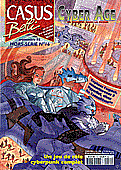
\includegraphics[width=4.00cm]{img/CouvCA.png}
\end{minipage} \hfill \begin{minipage}[ht]{14.50cm}
\textbf{Il y a quelques ann{\'e}es}, en 1990, la premi{\`e}re {\'e}dition de \emph{Cyber Age -- 30 minutes dans le futur}, permettait de jouer en fran\c{c}ais dans un univers de jeu de r{\^o}le cyberpunk. Les livres de Gibson avaient d{\'e}j{\`a} un bon succ{\`e}s, les films phares: \emph{Tron} et \emph{Blade Runner} {\'e}taient dans les m{\'e}moires et \emph{Total Recall} sur le point de sortir en France. TF1 {\'e}tait privatis{\'e}e, le Mur de Berlin tomb{\'e}. D'autres jeux cyberpunk apparurent en fran\c{c}ais, \emph{Cyber Age} n'{\'e}tait d{\'e}j{\`a} plus disponible.~\\

\textbf{Septembre 1995}, les mots invent{\'e}s par les cyberpunks sont entr{\'e}s dans le langage courant, les livres de Gibson sont des classiques, la presse et la t{\'e}l{\'e} nous ressassent le multiInternetautoroutem{\'e}dia, Bill Gates est l'homme le plus riche du monde, Traque sur Internet et Johnny Mnemonic viennent de sortir en France. \emph{Cyber Age -- 28 minutes dans le futur} est revenu en kiosque.~\\
\end{minipage}~\\

\textbf{Cyber Age} a chang{\'e}. L'encyclop{\'e}die est toujours l{\`a}, deux fois plus {\'e}paisse, vous permettant, m{\^e}me si vous ne jouez pas, de d{\'e}couvrir un univers cyberpunk. Les r{\`e}gles de \emph{Simulacres} sont ajout{\'e}es presque en int{\'e}gralit{\'e} pour avoir un jeu de r{\^o}le complet (ceux qui veulent des conseils pour d{\'e}buter devraient malgr{\'e} tout se procurer ce hors-s{\'e}rie). Les r{\`e}gles de \emph{Cyber Age} ont {\'e}t{\'e} revues. Trois sc{\'e}narios rempla\c{c}ent celui d'origine. Enfin, nous vous livrons directement quelques <<secrets>> de l'univers de \emph{Cyber Age} -- dans des pages {\`a} part -- plut{\^o}t que d'attendre des suppl{\'e}ment pour vous les r{\'e}v{\'e}ler.~\\

\textbf{Quoi de neuf donc ?} Le recyclage sans doute. Le cyberpunk a envahi le cin{\'e}ma, les s{\'e}ries t{\'e}l{\'e}, les jeux vid{\'e}os, les BD. \emph{Cyber Age} a emprunt{\'e} nombre de r{\'e}f{\'e}rences {\`a} de nombreux auteurs, mais des termes invent{\'e}s dans \emph{Cyber Age} ont eu aussi {\'e}t{\'e} repris {\`a} leur tour. Nos influences sont nombreuses, mais je voudrais signaler deux grandes sources malheureusement difficiles {\`a} trouver : la s{\'e}rie t{\'e}l{\'e} \emph{Max Headroom}, la BD anglaise (pas le film) \emph{Judge Dredd}. Le cyberpunk se cache partout. On croit le voir dans des films <<sp{\'e}cialis{\'e}s>> comme \emph{Le cobaye}, effroyablement mauvais. Et on le d{\'e}couvre dans \emph{Demolition Man}, film a priori gros bras et pourtant intelligent (avec la remarqu{\'e}e Sandra Bullock). Au d{\'e}tour d'une s{\'e}rie t{\'e}l{\'e} am{\'e}ricaine : \emph{Tek War}, on aper\c{c}oit une sc{\`e}ne de cyberspace meilleure que dans bien des films {\`a} gros budget ! Et Cl{\'e}o~\footnote{\texttt{http://www.canalplus.fr/}}, la cyberpr{\'e}sentatrice de Cyberflash, donne des nouvelles de la cyberculture tous les jours sur une cha{\^i}ne cybercrypt{\'e}e.~\\

\textbf{Mais}, que l'on lise \emph{Convoi\texttrademark} ou \emph{Carmen Mac Callum}, que l'on regarde \emph{Demolition Man} ou notre couverture, je vous le pr{\'e}dis: le h{\'e}ros du futur sera une h{\'e}ro{\"i}ne.~\\

\emph{Pierre Rosenthal}~\\

\textbf{PS}: Ah oui! L'encyclop{\'e}die de \emph{Cyber Age} est sur Internet ! Mais vous vous en {\'e}tiez rendu compte je pense... ~\\

Un index est pr{\'e}sent dans ce document page~\pageref{index}, notamment pour les termes not{\'e}s \texttt{comme ceci}. ~\\

Nouvelle mise en page (\LaTeX) / collation documentaire par Gabriel Chandesris, 01/08/2012-07/09/2012 ; avril-mai 2020. ~\\

\barreCyberAge

\begin{center}
	\begin{tabular}[ht]{ c c c c }
		\imgCANHfond	&	\imgCANHlogo	&	\imgCAMatrixTools	&	\imgCANTV555	\\
	\end{tabular}
\end{center}

\clearpage

\part*{Introduction\markboth{Introduction}{Introduction}}
\addcontentsline{toc}{part}{Introduction}
\label{Introduction}
\index{Introduction}

L'encyclop{\'e}die ci-apr{\`e}s est un m{\'e}lange de tout ce que l'on peut trouver sur le genre cyberpunk avec toutes sortes d'inventions propres {\`a} \emph{Cyber Age}. Les r{\'e}f{\'e}rences {\`a} des films, vid{\'e}os, livres, jeux ou bandes dessin{\'e}es sont l{\`a} pour vous aider {\`a} vous faire une id{\'e}e plus pr{\'e}cise des entr{\'e}es de l'encyclop{\'e}die. Une r{\'e}f{\'e}rence {\`a} un film ne veut pas dire que le film entier porte sur ce sujet, mais plut{\^o}t que l'on pourra y trouver une sc{\`e}ne, une ambiance ou un personnage illustrant ce point pr{\'e}cis. Les articles qui suivent sont -- bien s{\^u}r -- une petite s{\'e}lection tir{\'e}e de la \emph{Grande Encyclop{\'e}die du XXIe si{\`e}cle}, consultable sur le r{\'e}seau Avant Garde et le \texttt{network} CBS ou bien directement en \texttt{Interface} sous la r{\'e}f{\'e}rence \emph{GR ENCY LH 2080P}. Si, dans l'encyclop{\'e}die, vous trouvez plus loin les pictogrammes suivants...~\\ % , il vous suffira de cliquer dessus pour {\^e}tre guid{\'e} vers une liste de r{\'e}f{\'e}rences.~\\

\imgCALIVR Livres, \imgCABDBD Bandes dessin{\'e}es, \imgCACINE Cin{\'e}ma, \imgCATVTV T{\'e}l{\'e}vision, \imgCAJEUJ Jeux, \imgCATEKN Vie actuelle

~\\ \barreCyberAge

\begin{multicols*}{2}[\section*{Le monde en 2080\markboth{Le monde en 2080}{Le monde en 2080}}]
\addcontentsline{toc}{section}{Le monde en 2080}
\label{Monde2080}
\index{Monde2080@Monde en 2080, Le}

Les historiens modernes font remonter le d{\'e}but du \emph{Cyber Age} (l'{\^a}ge cybern{\'e}tique ou encore {\`e}re \texttt{cyberpunk}~\footnote{\textbf{CyberPunk} : Sous genre litt{\'e}raire de la science-fiction. Il m{\'e}lange futur proche, usage de la cybern{\'e}tique, des r{\'e}seaux informatiques, de la drogue. Ces th{\`e}mes {\'e}taient d{\'e}j{\`a} largement exploit{\'e}s par la science-fiction comme dans le pr{\'e}curseur \emph{Sur l'onde de choc} -- de John Brunner -- mais c'est le livre \emph{Neuromancien}, de William Gibson, qui a lanc{\'e} le genre. Il est {\`a} noter que le terme cyberpunk est post{\'e}rieur, et qu'il a depuis largement d{\'e}bord{\'e} son cadre en investissant les jeux vid{\'e}os, le cin{\'e}ma et les jeux de r{\^o}le. }) aux ann{\'e}es 2007, juste apr{\`e}s la Derni{\`e}re Guerre qui opposa pendant trois mois les USA et la Chine. La fin de cette guerre n'eut ni vainqueur ni vaincu, mais les destructions consid{\'e}rables, les pertes en vie humaines, et la conscience d'avoir {\'e}chapp{\'e} de peu au feu nucl{\'e}aire traumatis{\`e}rent les populations qui r{\'e}agirent en cons{\'e}quence. Les {\'E}tats furent rapidement mis en cause et d{\'e}mantel{\'e}s lors de la Grande R{\'e}volution Lib{\'e}rale qui suivit. Les grandes multinationales qui avaient pr{\'e}cis{\'e}ment contribu{\'e} {\`a} d{\'e}clencher la guerre puis {\`a} la faire cesser devinrent les structures dominantes du monde moderne. Les \texttt{TechnoBlocs} remplac{\`e}rent les {\'E}tats, mais leur emprise fut plus diffuse, plus m{\'e}thodique aussi. Certains chercheurs vont jusqu'{\`a} comparer l'{\`e}re moderne au Moyen {\^A}ge occidental o{\`u} toute la population vivait sous la coupe de seigneurs et de barons li{\'e}s entre eux par les lois de la f{\'e}odalit{\'e}, ou plus pr{\'e}cis{\'e}ment aux {\'E}tats nations des villes marchandes italiennes de la Renaissance. On peut effectivement trouver des ressemblances. {\`A} de tr{\`e}s rares exceptions, tout homme est inf{\'e}od{\'e} {\`a} un groupe plus ou moins important, qui lui-m{\^e}me a sa place dans le tissu {\'e}conomique. La seule loi que conna{\^i}t cet humain c'est la loi de son groupe, de son clan, que ce soit une bande de \texttt{tagueurs} ou un puissant \texttt{TechnoBloc}. Il doit ob{\'e}issance {\`a} son groupe, vit par lui et {\`a} travers lui. On peut bien entendu remarquer qu'un tel fonctionnement social avait d{\'e}j{\`a} exist{\'e} par le pass{\'e}, c'est le mode de fonctionnement de la soci{\'e}t{\'e} japonaise, ce n'est sans doute pas un hasard. Les structures du monde sont r{\'e}duites {\`a} quelques {\'e}quations simples d{\'e}j{\`a} pr{\'e}sentes dans le monde du XXe si{\`e}cle. Le pouvoir c'est le profit, le profit c'est l'information et la vente, la loi c'est celle de l'offre et de la demande. Tout est permis tout est possible mais il faut gagner. Les concepts de moralit{\'e}, d'ind{\'e}pendance, de justice et d'{\'e}galit{\'e} n'ont plus cours. Mais certains chercheurs ajoutent aussit{\^o}t : ont-ils jamais exist{\'e} par le pass{\'e} ? %% ~\\

\section*{Histoire\markboth{Histoire}{Histoire}}
\addcontentsline{toc}{section}{Histoire}
\label{Histoire}
\index{Histoire}

\begin{itemize}
	\item[\textbf{2001}] : fin des guerres am{\'e}ricaines entre les USA, l'Union d'Am{\'e}rique Centrale (U.A.C.) et le Mexique. Fin du leadership am{\'e}ricain dans le monde, retour au protectionnisme de Washington, apparition de la premi{\`e}re \texttt{Zone Blanche} (NOrd MExique/TExas: NOMETA). Confirmation du r{\^o}le leader du Japon qui impose la paix. Fin de l'anarchie dans l'ex URSS dont les nouvelles fronti{\`e}res se stabilisent.
	\item[\textbf{2005}] : guerre nucl{\'e}aire au Moyen Orient entre l'Iran et l'Arabie Saoudite (soutenue par Isra{\"e}l et l'{\'E}gypte) pour le contr{\^o}le des lieux saints et des champs de p{\'e}trole encore en activit{\'e}. Guerre qui entra{\^i}ne la premi{\`e}re r{\'e}volution lib{\'e}rale restreignant consid{\'e}rablement le pouvoir des {\'E}tats. Formation de la seconde \texttt{Zone Blanche} (M{\'e}sopotamie: MESO).
	\item[\textbf{2007}] : la tentative de reconstruction de la Grande Pologne prend fin suite {\`a} la d{\'e}faite de l'arm{\'e}e polonaise devant Kiev face aux unit{\'e}s de partisans ukrainiens soutenus par la r{\'e}publique de Grande Russie, les volontaires des r{\'e}publiques Baltes et les anciens {\'e}l{\'e}ments de l'Arm{\'e}e Rouge. Apparition d'une troisi{\`e}me \texttt{Zone Blanche} (BAltique/POlogne: BAPO).
	\item[\textbf{2010}] : le Grand Choc manque engloutir la Californie dans le Pacifique.
	\item[\textbf{2015}] : formation des premiers \texttt{TechnoBlocs}, les \texttt{Sept Dragons}: Avant Garde, Lumi{\`e}re Coh{\'e}rente, IBM, Matsushita, Mitsubishi/Benz, CGE/Philips, Sony. Les deux premiers Dragons {\'e}tant les multinationales qui construiront dans l'espace les \texttt{{\^I}les de la Lune} -- Premi{\`e}res \texttt{{\'E}meutes de la faim}.
	\item[\textbf{2018}] : d{\'e}but des guerres priv{\'e}es (entre cha{\^i}nes de restaurants). Cr{\'e}ation de la \texttt{L{\'e}gion Cerb{\`e}re}.
	\item[\textbf{2023}] : mise en service des \texttt{{\^I}les de la Lune}.
	\item[\textbf{2027}] : autodissolution de l'ONU qui laisse la place au grand conseil f{\'e}d{\'e}ral des \texttt{TechnoBlocs} (abr{\'e}viation: Grand Conseil ou G.C.).
	\item[\textbf{2030}] : deuxi{\`e}me grande r{\'e}volution lib{\'e}rale. {\'E}diction des lois f{\'e}d{\'e}rales, ouverture du grand march{\'e} mondial, abolition des fronti{\`e}res, les gouvernements et les {\'E}tats n'ont plus qu'une t{\^a}che d'entretien.
	\item[\textbf{2031}] : les nationalit{\'e}s s'effacent peu {\`a} peu, un homme n'est plus d{\'e}fini par son pays mais par le \texttt{TechnoBloc} auquel il appartient, souvent {\`a} vie.
\end{itemize}~\\

Apr{\`e}s l'{\'e}limination des principaux gangs mondiaux vers la fin des ann{\'e}es 90, le monde du crime s'est reform{\'e} sous la domination de deux grandes forces: le \texttt{yakuza} (d'origine japonaise) et les \texttt{triades} (d'origine chinoise), la maffia russe venant en troisi{\`e}me position. S'adaptant au monde du XXIe si{\`e}cle, ces deux organisations ont maintenant pignon sur rue, on peut y faire carri{\`e}re comme dans n'importe quelle multinationale. On parle d'ailleurs des Deux Dragons en r{\'e}f{\'e}rence aux \texttt{Sept Dragons} qui forment les sept groupes industriels les plus puissants du monde. Les Deux Dragons ont chacun une organisation infaillible et redoutable qui couvre tous les trafics illicites de la Terre, leurs milices sont tr{\`e}s entra{\^i}n{\'e}es et capables de tenir t{\^e}te, en hommes et en armement, {\`a} n'importe quel autre groupe du m{\^e}me genre. Les Deux Dragons tol{\`e}rent quelques malfrats ind{\'e}pendants mais leur {\'e}thique est tr{\`e}s stricte, {\`a} la moindre trahison ils frappent sans piti{\'e} et {\'e}liminent le malheureux quel qu'en soit le prix; c'est sans doute pour cette raison qu'ils sont tant craints et respect{\'e}s. Les Deux Dragons sont concurrents et donc ennemis, et se livrent une guerre sans merci.~\\

\vfill ~\\ \columnbreak

Les milices ont remplac{\'e} les arm{\'e}es des {\'E}tats apr{\`e}s la Derni{\`e}re Guerre. Mais {\`a} l'instar de ces arm{\'e}es, les milices, qui appartiennent aux grands groupes industriels, op{\`e}rent {\`a} longueur d'ann{\'e}es dans autant de mini guerres priv{\'e}es. Toutes les milices ont donc un statut l{\'e}gal et leurs op{\'e}rations sont reconnues par tout le monde pour peu qu'un {\'e}tat de guerre {\'e}conomique ait {\'e}t{\'e} d{\'e}clar{\'e} au pr{\'e}alable, bien que de multiples exemples d'attaques sans d{\'e}claration en pr{\'e}avis puissent {\^e}tre trouv{\'e}s. Les milices existent aussi sous des formes ind{\'e}pendantes: les \texttt{Mercenaires} ou les Forces {\'E}clairs, leurs {\'e}tats-majors se louant au plus offrant. Les guerres entre milices peuvent prendre toutes les formes, de l'affrontement d{\'e}clar{\'e} en champs clos jusqu'aux op{\'e}rations de sabotage, de commando contre des cibles particuli{\`e}res ou l'\texttt{exfiltration}~\footnote{\textbf{Exfiltration} : C'est le contraire de l'infiltration. Il faut faire s'{\'e}chapper quelqu'un du \texttt{TechnoBloc} auquel il appartient. } d'un cadre particuli{\`e}rement brillant d'un \texttt{TechnoBloc} concurrent. La seule r{\`e}gle que doivent respecter les {\'e}tats-majors des milices est de ne pas employer d'armes atomiques ou bact{\'e}riologiques sous peine de se voir irr{\'e}m{\'e}diablement d{\'e}truite par la coalition de toutes les autres milices. Ce fut le cas, et c'est le seul exemple, pour la milice Thastubha de New Yokohama. Le propri{\'e}taire de la milice fut alors d{\'e}clar{\'e} hors la loi et disparut avec elle. Les milices ont un classement annuel recens{\'e} dans \emph{Faits Strat{\'e}giques \& {\'E}conomiques}. Les r{\'e}dacteurs de cette c{\'e}l{\`e}bre revue ind{\'e}pendante {\'e}valuent l'efficacit{\'e} des milices lors de l'ann{\'e}e pass{\'e}e {\`a} partir des derniers affrontements. Les meilleures milices, outre la Force {\'E}clair Delta, sont pour cette ann{\'e}e 2080 les forces de la New Tech IBM et celles de la Tokohama inc. Les milices des \texttt{yakuzas~} et des \texttt{triades} n'ont jamais pu {\^e}tre {\'e}valu{\'e}es correctement mais les sp{\'e}cialistes s'accordent pour dire qu'elles doivent ais{\'e}ment se placer dans les cinq premi{\`e}res places. Un officier dans une milice d'{\'e}lite a le rang et le salaire d'un cadre sup{\'e}rieur et les chasseurs de t{\^e}tes leur font sans cesse des offres tr{\`e}s all{\'e}chantes pour leur faire quitter leur groupe pour un autre.~\\

\textbf{R{\'e}f{\'e}rence}
\begin{itemize}
	\small
	\item \imgCACINE \emph{Yakuza}, de Sydney Pollack (1974), avec Robert Mitchum et Ken Takakura.
	\item \imgCACINE \emph{Black Rain}, de Ridley Scott (1989), avec Michael Douglas et Ken Takakura. 
\end{itemize}

\end{multicols*}

%% \barreCyberAge
\clearpage

\begin{multicols*}{2}

\part*{Politique\markboth{Politique}{Politique}}
\addcontentsline{toc}{part}{Politique}
\label{Politique}
\index{Politique}

\section*{Les Sept Dragons/TechnoBlocs\markboth{Les Sept Dragons/TechnoBlocs}{Les Sept Dragons/TechnoBlocs}}
\addcontentsline{toc}{section}{Les Sept Dragons/TechnoBlocs}
\label{SeptDragons}
\index{SeptDragons}
\label{TechnoBlocs}
\index{TechnoBlocs}

Il s'agit l{\`a} du terme d{\'e}signant les sept \texttt{TechnoBlocs} les plus puissants du moment. Une puissance, un \texttt{Dragon}, ou un \texttt{TechnoBloc} est un ensemble d'entreprises r{\'e}unies en trust. C'est le si{\`e}ge du pouvoir. En fin de compte, et malgr{\'e} une multitude d'{\'e}crans et de soci{\'e}t{\'e}s paravent, il est certain que tout humain travaille pour un des \texttt{Sept Dragons} sans le savoir. ~\\

Les \texttt{Sept Dragons} ont leurs si{\`e}ges sociaux dans les \texttt{{\^I}les de la Lune}, ce qui les met {\`a} l'abri des guerres priv{\'e}es. Pour {\^e}tre accueilli dans le cercle tr{\`e}s ferm{\'e} des Dragons il faut d'ailleurs imp{\'e}rativement pouvoir ouvrir son si{\`e}ge en orbite de la Terre. Les \texttt{TechnoBlocs}, {\`a} bien des {\'e}gards, ressemblent aux {\'E}tats du XXe si{\`e}cle, ou plut{\^o}t aux principaut{\'e}s marchandes de l'Italie de la Renaissance. Ils poss{\`e}dent leurs propres arm{\'e}es, leurs polices, leurs services d'espionnage et de contre-espionnage, leurs lois et leurs dirigeants. Leur but unique et commun est de faire du profit et de prot{\'e}ger leur existence. En cela encore, ils ne se diff{\'e}rencient pas vraiment des nations de l'ancien monde. Un \texttt{TechnoBloc} est souverain sur son territoire, c'est pour cette raison que chacun entretient des missions diplomatiques aupr{\`e}s des autres Dragons. Certains \texttt{TechnoBlocs} professent une id{\'e}ologie propre et il est n{\'e}cessaire d'y souscrire pour y travailler, d'autres non. %% ~\\

\section*{D{\'e}mocratie\markboth{D{\'e}mocratie}{D{\'e}mocratie}}
\addcontentsline{toc}{section}{D{\'e}mocratie}
\label{Democratie}
\index{Democratie}
%% \pageREFtoTechnoBlocs

Une des cons{\'e}quences de la mont{\'e}e en puissance des \texttt{TechnoBlocs} fut la fin des d{\'e}mocraties dans le monde. Un syst{\`e}me d{\'e}mocratique demande un {\'E}tat ind{\'e}pendant et impartial mais dans le monde du XXIe si{\`e}cle, aucune structure n'{\'e}chappe {\`a} la d{\'e}pendance de la soci{\'e}t{\'e} du spectacle et au spectacle de la soci{\'e}t{\'e}. Les deux ma{\^i}tres {\'e}talons de la soci{\'e}t{\'e} moderne, l'argent et le spectacle ont d{\^u} inventer une nouvelle rengaine pour remplacer celle du pain et des jeux. ~\\

Mais qu'on ne s'y trompe pas, le nouvel ordre spectaculaire n'a pas aboli toute id{\'e}e de libert{\'e}. Au contraire, en se glissant entre les mailles du filet des \texttt{TechnoBlocs} on peut trouver plus de plages de libert{\'e} que dans les vieilles soci{\'e}t{\'e}s de la fin du XXe si{\`e}cle. Mais voil{\`a}, de quoi s'agit-il vraiment? On parle d'ind{\'e}pendance, de nouvelles r{\`e}gles du jeu, de failles, mais peut-{\^e}tre n'est-ce pas la m{\^e}me chose et c'est vrai que la libert{\'e} formul{\'e}e n'est plus un concept moderne utilis{\'e} de nos jours. %% ~\\

\section*{Id{\'e}ologie\markboth{Id{\'e}ologie}{Id{\'e}ologie}}
\addcontentsline{toc}{section}{Id{\'e}ologie}
\label{Ideologie}
\index{Ideologie@Id{\'e}ologie}

Le terme d'id{\'e}ologie regroupe les croyances religieuses et politiques du XXIe si{\`e}cle.Tout le monde peut fonder une {\'e}glise, un parti ou une secte, la d{\'e}mocratie s'applique au monde entier. Les croyants d'un m{\^e}me groupe peuvent s'organiser pour vivre ensemble. Dans l'enceinte du groupe, les lois internes seront prioritaires sur celles de l'ext{\'e}rieur. On conna{\^i}t dans un m{\^e}me endroit plusieurs communaut{\'e}s vivant en bonne intelligence mais ob{\'e}issant {\`a} leurs r{\`e}gles. Une infraction commise au sein d'une communaut{\'e} est jug{\'e}e par les instances de cette communaut{\'e}. Il existe des lois f{\'e}d{\'e}rales (un peu {\`a} la mani{\`e}re des anciens USA) qui ont le pas sur les lois communautaires, il s'agit la plupart de temps de crimes de sang ou assimil{\'e}s. ~\\

Cette libert{\'e} de conscience, associ{\'e}e aux moyens d'information modernes et {\`a} l'{\'e}croulement des anciennes valeurs du XXe si{\`e}cle, a permis l'{\'e}mergence de toutes sortes de sectes plus {\'e}tranges les unes que les autres mais poss{\'e}dant un statut pour peu qu'elles soient prises en charge par un \texttt{TechnoBloc}. %% ~\\

\section*{Les guildes et les alliances\markboth{Les guildes et les alliances}{Les guildes et les alliances}}
\addcontentsline{toc}{section}{Les guildes et les alliances}
\label{GuildesAlliances}
\index{Guildes@Guildes et Alliances}
\index{Alliances@Alliances et Guildes}

La mondialisation de l'{\'e}conomie a cr{\'e}{\'e} le principe des guildes (ou hanses) et des alliances, plusieurs groupes unissant leurs forces et s'interconnectant pour conqu{\'e}rir ou garder un march{\'e}, une part de march{\'e} ou une influence politique. Une guilde est un macro ensemble {\'e}conomique. Une alliance est un macro ensemble politique (comme l'Europe).~\\

Les guildes ont donn{\'e} naissance aux \texttt{TechnoBlocs} qui sont comme des villes {\'e}tats. Les nationalit{\'e}s, les ensembles supranationaux, les <<alliances>>, th{\'e}oriquement au-dessus des guildes n'ont qu'un pouvoir factuel sur ces derni{\`e}res.~\\

En dehors des sept groupes supranationaux il existe {\'e}galement plusieurs dizaines d'{\'e}tats encore constitu{\'e}s en tant que tels mais ils ne p{\`e}sent pas lourd dans les n{\'e}gociations mondiales. Il s'agit d'anciens pays du tiers monde qui n'ont pas pu prendre {\`a} temps le virage de la <<Troisi{\`e}me Vague>> ou de territoires refusant clairement le principe des alliances comme la F{\'e}d{\'e}ration Libertaire de Micron{\'e}sie, le \texttt{califat de Carthage} ou la dictature {\'e}cologique de Malaisie. ~\\

Les ensembles supra nationaux -- les alliances -- n'ont aucun pouvoir {\'e}conomique, ils sont par contre responsables de la s{\'e}curit{\'e}. Les forces arm{\'e}es n'existant plus, il s'agit de forces de police et de maintien de l'ordre. ~\\

Un homme peut donc avoir une double nationalit{\'e}, celle de son ensemble d'origine ou de son pays, et celle de son \texttt{TechnoBloc}. Le syst{\`e}me est tr{\`e}s proche de celui des villes {\'e}tats allemandes durant la Renaissance. Il doit respecter les lois de l'ensemble dans lequel il vit mais {\'e}galement celles du \texttt{TechnoBloc} dans lequel il {\'e}volue. Un homme peut {\'e}galement n'avoir qu'une seule identit{\'e}, celle de son pays ou de son alliance; et n'appartenir {\`a} aucun \texttt{TechnoBloc}. Mais c'est une situation peu enviable, il s'agit la plupart du temps de citoyen de troisi{\`e}me zone. ~\\

Les alliances doivent passer par la convocation de di{\`e}tes pour fixer leur budget et le cadre de leur activit{\'e} comme le <<conseil des sages>> pour la f{\'e}d{\'e}ration GreatAsia, ou l'Europarlement pour l'alliance EuroCom. %% ~\\

\section*{Crime f{\'e}d{\'e}ral\markboth{Crime f{\'e}d{\'e}ral}{Crime f{\'e}d{\'e}ral}}
\addcontentsline{toc}{section}{Crime f{\'e}d{\'e}ral}
\label{CrimeFederal}
\index{CrimeFederal@Crime f{\'e}d{\'e}ral}

La notion de crime f{\'e}d{\'e}ral est directement issue du syst{\`e}me des \texttt{TechnoBlocs}. Apr{\`e}s une premi{\`e}re p{\'e}riode d'ultralib{\'e}ralisme, les \texttt{Sept Dragons~} se r{\'e}unirent pour {\'e}tablir une charte de crimes passibles du d{\'e}p{\^o}t de bilan pour les soci{\'e}t{\'e}s convaincues du d{\'e}lit, y compris par la force si le besoin s'en faisait sentir. Parmi les crimes f{\'e}d{\'e}raux {\'e}tablis par les \texttt{Sept Dragons} on peut signaler: l'usage des \texttt{Vid{\'e}oDrogues}, l'usage ou le stockage d'armes atomiques, le lancement d'une op{\'e}ration militaire en direction d'un des \texttt{{\^I}les de la Lune} ; et enfin, l'accroissement d'autonomie des \texttt{Intelligences Artificielles} et leur {\'e}veil {\`a} la conscience. %% ~\\

\section*{Naissance des unit{\'e}s Cr{\'e}puscule\markboth{Naissance des unit{\'e}s Cr{\'e}puscule}{Naissance des unit{\'e}s Cr{\'e}puscule}}
\addcontentsline{toc}{section}{Naissance des unit{\'e}s Cr{\'e}puscule}
\label{UnitesCrepuscules}
\index{UnitesCrepuscules@Unit{\'e}s Cr{\'e}puscule, Naissance des ...}
\index{Crepuscules@Cr{\'e}puscule, Naissance des unit{\'e}s ...}

La premi{\`e}re grande perc{\'e}e en mati{\`e}re d'Intelligence Artificielle (\texttt{I.A.}) vint des laboratoires ATTR de Kyoto {\`a} la fin du si{\`e}cle dernier; lorsque les chercheurs regroup{\'e}s sous la direction de professeur Hugo de Glaris parvinrent {\`a} fabriquer un r{\'e}seau neuronal disposant d'un nombre de synapses sup{\'e}rieur au cerveau humain. ~\\

Vers 2015 des bioneurones artificiels/naturels permirent de voir {\'e}merger une forme d'intelligence artificielle concr{\`e}te. Des journalistes lanc{\`e}rent alors une boutade: <<si les cerveaux de silicium mis au point {\`a} Kyoto {\'e}taient plus puissants que le cerveau humain, plus gros, plus interconnect{\'e}s, disposant de plus de neurones et de synapses, alors ne devait-on pas les consid{\'e}rer comme une nouvelle esp{\`e}ce, sup{\'e}rieure {\`a} l'homme, la race {\`a} venir?>> Ils ne croyaient pas si bien dire et c'est moins de cinq ans plus tard qu'on commen\c{c}a {\`a} s'en apercevoir, ainsi naquirent les \texttt{unit{\'e}s Cr{\'e}puscule}. Elles avaient pour mission de faire en sorte que les propos des journalistes ne se transforment pas en r{\'e}alit{\'e}. ~\\

\vfill ~\\ %% \columnbreak

D{\`e}s qu'une \texttt{Intelligence Artificielle} disposant de l'autonomie de pens{\'e}e et d'action est d{\'e}tect{\'e}e, les \texttt{unit{\'e}s Cr{\'e}puscule} sont envoy{\'e}es pour <<r{\'e}soudre>> le probl{\`e}me. Les \texttt{unit{\'e}s Cr{\'e}puscule} sont, avec la \texttt{L{\'e}gion Cerb{\`e}re}, les seuls organismes InterTechnoBlocs, leurs op{\'e}rations sont tr{\`e}s discr{\`e}tes, elles ne recherchent pas la publicit{\'e}, leurs sentences sont sans appel et leur ex{\'e}cution s (g{\'e}n{\'e}ralement la mort pour le ou les humains responsables et la destruction des m{\'e}moires de l'I.A.) sont imm{\'e}diates. ~\\

Plusieurs \texttt{networks} ont essay{\'e} de produire des reportages sur les \texttt{unit{\'e}s Cr{\'e}puscule} mais aucun n'y est parvenu, soit que l'{\'e}quipe de tournage ait d{\^u} subir de myst{\'e}rieux attentats, soit que le network lui-m{\^e}me ait {\'e}t{\'e} la cible d'une O.P.A. foudroyante visant {\`a} le racheter et {\`a} changer toute sa grille de programmes. ~\\

Pour certains commentateurs les \texttt{unit{\'e}s Cr{\'e}puscule} ne sont qu'une l{\'e}gende, c'est d'ailleurs la position de tous les services de communication de tous les grands \texttt{TechnoBlocs}. %% ~\\

\section*{{\'E}meutes de la faim\markboth{{\'E}meutes de la faim}{{\'E}meutes de la faim}}
\addcontentsline{toc}{section}{{\'E}meutes de la faim}
\label{EmeutesFaim}
\index{EmeutesFaim@{\'E}meutes de la faim}

S{\'e}ries d'{\'e}meutes dans les grandes villes des cinq continents qui d{\'e}g{\'e}n{\`e}rent en guerres civiles dans de nombreux endroits (New York, Rio, Afrique du Sud, Mexique, Espagne, Italie, sud de la France) et n{\'e}cessit{\`e}rent l'envoi de troupes interblocs (la \texttt{L{\'e}gion Cerb{\`e}re}) pour r{\'e}tablir f{\'e}rocement l'ordre dans la rue. Ces {\'e}meutes eurent de graves cons{\'e}quences sur le monde moderne. %% ~\\
\begin{itemize}
	\item[$\bullet$] {\'E}tablissement d'un plan de survie par le Conseil G{\'e}n{\'e}ral pour toutes les populations du Tiers-monde afin de les maintenir juste au-dessus du seuil de subsistance.
	\label{CeinturesFaim}
	\index{CeinturesFaim@Ceintures de la Faim}
	\item[$\bullet$] Bouclage des fronti{\`e}res des pays d{\'e}velopp{\'e}s (la \texttt{Ceinture de la faim}).
	\item[$\bullet$] Abandon de tous les plans de d{\'e}veloppement en faveur du Tiers-monde.
	\item[$\bullet$] D{\'e}but des grandes vagues d'attentats terroristes par les ressortissants de ces m{\^e}mes pays. Un commentateur put dire {\`a} l'{\'e}poque: <<La moiti{\'e} de l'humanit{\'e} d{\'e}cide froidement d'abandonner l'autre, personne ne peut en pr{\'e}dire les cons{\'e}quences>>.
\end{itemize}~\\

\textbf{R{\'e}f{\'e}rence}
\begin{itemize}
	\small
	\item \imgCATVTV \emph{No man's land}, de Ben Bolt (1994) pour la BBC/arte, avec Trevor Eve et Amanda Ooms.
	% TODO ajouter : 
	% Aqua\texttrademark, Jean-Marc Ligny, Pr{\'e}sence du Futur
	% Jihad, Jean-Marc Ligny, Pr{\'e}sence du Futur
\end{itemize}

\vfill ~\\ \columnbreak

\section*{Zone Blanche\markboth{Zone Blanche}{Zone Blanche}}
\addcontentsline{toc}{section}{Zone Blanche}
\label{ZoneBlanche}
\index{ZoneBlanche@Zone Blanche}

On trouve plusieurs grandes \texttt{Zones Blanches} sur la Terre. a premi{\`e}re {\`a} la fronti{\`e}re de l'ancien Mexique et du Texas et l'autre sur les c{\^o}tes de la Baltique {\`a} la hauteur de l'ancienne Pologne. Il s'agit d'{\'e}tendues d{\'e}sertiques, st{\'e}rilis{\'e}es par les bombes nucl{\'e}aires et les programmes g{\'e}n{\'e}tiques des derni{\`e}res guerres inter {\'E}tats de la fin du XXe si{\`e}cle. On ne peut y vivre longtemps sans subir des mutations tr{\`e}s souvent mortelles. Les \texttt{networks} y organisent des courses d'hovertanks. Les \texttt{Zones Blanches} sont aussi le repaire de tous les proscrits, et les mutants qui y cherchent un ultime refuge. Il existe bien d'autres \texttt{Zones Blanches} sur la Terre mais aucune n'est aussi vaste que celles cit{\'e}es plus haut. Les \texttt{Zones Blanches} sont les seuls territoires qui {\'e}chappent au contr{\^o}le des \texttt{TechnoBlocs}. On y survit sous le joug d'une autre loi, la loi de la jungle, et pour tout dire, pas tr{\`e}s longtemps. %% ~\\

\textbf{R{\'e}f{\'e}rence}
\begin{itemize}
	\small
	\item \imgCALIVR \emph{C{\^a}bl{\'e}}, Walter Jon Williams, Pr{\'e}sence du futur.
	\item \imgCALIVR \emph{Les culbuteurs de l'enfer}, Roger Zelazny, Titres SF.
	\item \imgCALIVR \emph{Le marteau de verre}, K.W. Jeter, Pr{\'e}sence du futur.
	\item \imgCABDBD \emph{Judge Dredd}, The Cursed Earth, Titan Books.
	\item \imgCACINE \emph{Point Limite Z{\'e}ro}, de Richard Sarafian (1971), avec Barry Newman.
\end{itemize}

\section*{Tiers-monde\markboth{Tiers-monde}{Tiers-monde}}
\addcontentsline{toc}{section}{Tiers-monde}
\label{TiersMonde}
\index{TiersMonde@Tiers-monde}

Quatre sous-continents sont exclus du d{\'e}veloppement moderne du XXIe si{\`e}cle. Il s'agit de l'Afrique dans son immense majorit{\'e}, de l'Inde et de la Chine (bien que plus d{\'e}velopp{\'e}es que le continent noir) ainsi que l'Asie Centrale. Dans tous ces espaces, la vie est encore souvent {\`a} l'image du XXe si{\`e}cle voire du XIXe. Si la famine n'est plus qu'un ph{\'e}nom{\`e}ne exceptionnel (suite aux graves {\'E}meutes de la faim). Les millions d'habitants qui peuplent ces contr{\'e}es mangent tout juste {\`a} leur faim. La fermeture des fronti{\`e}res de l'Europe du Nord dans les ann{\'e}es 2010, et le renforcement de cette ceinture par la cr{\'e}ation de la \texttt{L{\'e}gion Cerb{\`e}re} contribua {\`a} couper d{\'e}finitivement le monde en deux et engendra un immense sentiment de haine et de frustration dans les pays du Tiers-monde. D'o{\`u} la naissance de nombreux groupes terroristes {\`a} caract{\`e}re nihiliste cherchant {\`a} s'infiltrer au-del{\`a} de la \texttt{Ceinture de la faim} pour y porter la violence. En {\'e}change du plan de subsistance, les populations du Tiers-monde doivent se plier de gr{\'e} ou de force {\`a} un plan de contr{\^o}le des naissances.~\\

La technologie du cyberspace n'y est que tr{\`e}s rarement employ{\'e}e et les r{\'e}seaux de communication y sont embryonnaires. On ne peut se brancher sur le \texttt{R{\'e}zo} que dans les grands h{\^o}tels internationaux ou dans les grands centres de vacances organis{\'e}es. ~\\

Il s'agit toujours de lieux ultra surveill{\'e}s, des camps retranch{\'e}s de luxe interdits aux indig{\`e}nes, ou dans le meilleur des cas autoris{\'e}s aux castes les plus riches. ~\\

\textbf{R{\'e}f{\'e}rence}
\begin{itemize}
	\small
	\item \imgCATVTV \emph{No man's land}, de Ben Bolt (1994) pour le BBC, avec Trevor Eve et Amanda Ooms.
	\item \imgCABDBD \emph{Froid {\'E}quateur}, d'Enki Bilal, Dargaud.
	\item \imgCACINE \emph{Soleil Vert}, de Richard Fleischer, avec Charlton Heston.
\end{itemize}

\section*{Les Venises\markboth{Les Venises}{Les Venises}}
\addcontentsline{toc}{section}{Les Venises}
\label{Venises}
\index{Venises@Venises, Les}

Ce n'est qu'au milieu du XXIe si{\`e}cle qu'on commen\c{c}a {\`a} s'occuper s{\'e}rieusement des exploitations sous-marines. Il faut dire que cette fois on avait de nombreuses raisons pour se pencher sur le Grand Bleu. La surpopulation, la pollution des c{\^o}tes, le r{\'e}chauffement du climat, toutes ces catastrophes pr{\^e}chaient pour l'{\'e}tablissement de l'homme dans un milieu oc{\'e}anique de la m{\^e}me fa\c{c}on qu'il commen\c{c}ait {\`a} le faire dans l'espace.~\\

Ainsi naquirent les premi{\`e}res \texttt{Venises}. On les baptisa sans doute de cette fa\c{c}on {\`a} cause des premi{\`e}res tentatives d'{\'e}tablissements qui se firent dans l'Adriatique, non loin de la cit{\'e} des Doges. On comprit tr{\`e}s vite que les \texttt{Venises} pouvaient {\^e}tre la source d'un juteux profit: fermes aquatiques, extractions des nodules riches en minerai qui jonchaient les plaines abyssales, tourisme de luxe, p{\^e}che. En l'espace de quelques ann{\'e}es on compta bient{\^o}t une douzaine de cit{\'e}s marines, une douzaine de Venises. Elles ob{\'e}issaient toutes {\`a} un sch{\'e}ma identique : chaque \texttt{Venise} {\'e}tait ind{\'e}pendante (comme un \texttt{TechnoBloc}) et mieux encore car au terme de plusieurs proc{\`e}s retentissants on consid{\'e}ra les \texttt{Venises} comme de pleins {\'e}tats ind{\'e}pendants. En fait, on reconnut rapidement que les \texttt{Venises} n'{\'e}taient ni plus ni moins que de nouvelles {\^i}les {\`a} la surface du globe.~\\

Une \texttt{Venise} veille jalousement sur son territoire, implantant des modules ind{\'e}pendants parfois loin de ses c{\^o}tes. Fermes aquatiques, usines d'extractions de nodules, toutes les activit{\'e}s industrielles en haute mer d{\'e}pendent des \texttt{Venises}. La plupart de ces {\^i}les en <<thermociment>> tirent leur {\'e}nergie de gigantesques capteurs solaires flottants: les <<N{\'e}nuphars>>, implant{\'e}s {\`a} quelques kilom{\`e}tres de leurs c{\^o}tes. Situ{\'e}es dans des zones d'ensoleillement maximum, les N{\'e}nuphars alimentent les \texttt{Venises} en {\'e}nergie propre. Et c'est la seconde grande caract{\'e}ristique des \texttt{Venises} : l'immense majorit{\'e} de leurs habitants sont des {\'e}cologistes convaincus. On vient sur une \texttt{Venise} car on consid{\`e}re que les continents pollu{\'e}s ne peuvent plus accueillir l'homme, c'est un choix de soci{\'e}t{\'e} et de vie.~\\

Un journaliste compara les premi{\`e}res \texttt{Venises} aux {\'e}tablissements hippies de la fin des ann{\'e}es 1960 et c'est vrai qu'on y retrouve le m{\^e}me {\'e}tat d'esprit. Ce qui n'emp{\^e}che pas plusieurs forces \texttt{Merc} directement issu des \texttt{Venises} d'{\^e}tre class{\'e}es en championnat, sur les \texttt{Venises} comme partout dans le monde, la non-violence est un concept de moins en moins partag{\'e}.~\\

\label{Tritons}
\index{Tritons}
Les parties sous-marines des \texttt{Venises} sont parfois d{\'e}nomm{\'e}es aquavilles. Bien que vivant sous d{\^o}me pressuris{\'e}, certains habitants des aquavilles se font greffer des branchies externes. On les appelle \texttt{Tritons}, ou Sir{\`e}nes. Les apprentis pilotes, ou les futurs colons spatiaux, viennent souvent faire des stages en aquaville avant de partir en \texttt{Espace profond}.~\\

\textbf{R{\'e}f{\'e}rence}
\begin{itemize}
	\small
	\item \imgCATVTV \emph{SeaQuest DSV}, produit par Steven Spielberg (1993).
	\item \imgCACINE \emph{Waterworld}, de Kevin Reynolds (1995), avec Kevin Costner et Dennis Hopper.
\end{itemize}

\vfill

\section*{Le califat de Carthage\markboth{Le califat de Carthage}{Le califat de Carthage}}
\addcontentsline{toc}{section}{Le califat de Carthage}
\label{CalifatCarthage}
\index{CalifatCarthage@Califat de Carthage, Le}

Les modifications climatiques et les deux guerres civiles et religieuses qui ont amen{\'e} le califat au pouvoir n'ont pas laiss{\'e} beaucoup de choix politique {\`a} l'ancien Maghreb. Le califat s'{\'e}tend du Maroc {\`a} l'ex Libye, c'est une des derni{\`e}res structures {\'e}tatiques existante au monde, c'est aussi une dictature islamique.~\\

Les principales sources de revenus du califat sont la contrebande et le recel de malfaiteurs.~\\

C'est en effet une des seules zones {\`a} ne pas respecter les accords interforces et interblocs. Un criminel recherch{\'e} pour \texttt{crime f{\'e}d{\'e}ral} peut, {\`a} condition d'avoir beaucoup d'argent, y trouver refuge. Les principales organisations et cartels de maffieux, les \texttt{triades}, les \texttt{yakuzas}, y ont pignon sur rue. Durant plusieurs si{\`e}cles les {\'E}tats Barbaresques avaient accueilli tous les corsaires, tous les pirates, tous les proscrits chr{\'e}tiens. Le califat est donc une sorte de retour aux sources, les autorit{\'e}s religieuses affirmant quant {\`a} elles que l'hospitalit{\'e} est un des commandements du Coran (ce qui est vrai).~\\

Pour qui n'a pas de gros moyens la vie est plut{\^o}t dure dans le califat mais il existe {\'e}galement beaucoup de palais magnifiques, herm{\'e}tiquement isol{\'e}s des rayons mortels du soleil, o{\`u} l'on vit comme dans un paradis en versant de confortables rentes aux agents du Calife.~\\

\vfill ~\\ \columnbreak

Il y a aussi des zones interdites, certains quartiers se d{\'e}fendant farouchement de l'intrusion des {\'e}trangers: ce sont les casbahs. Elles sont contr{\^o}l{\'e}es par des clans qui n'admettent pas qu'un roumi (homme blanc) vienne toucher un contrat sur la t{\^e}te d'un de leur h{\^o}te. Car si on vient dans le califat pour s'y cacher on y vient {\'e}galement pour chercher, traquer, et souvent abattre les fugitifs. Bab El K{\'e}bir est une de ces casbahs, un territoire ou tout {\'e}tranger non recommand{\'e} est virtuellement en passe de dispara{\^i}tre sans laisser de traces. On n'a jamais entendu parl{\'e} d'un contrat honor{\'e} {\`a} Bab El K{\'e}bir et ceux qui ont essay{\'e} ne sont jamais ressortis de ses ruelles blanches.~\\

Les \texttt{Sept Dragons} essayent depuis des ann{\'e}es de prouver que le califat d{\'e}tient une \texttt{I.A.} ill{\'e}gale, afin d'y envoyer les \texttt{unit{\'e}s Cr{\'e}puscules}. Le sourire kabyle semble {\^e}tre la seule r{\'e}ponse qu'ils ont obtenu jusqu'{\`a} pr{\'e}sent.~\\

\textbf{R{\'e}f{\'e}rence}
\begin{itemize}
	\small
	\item \imgCALIVR \emph{Gravit{\'e} {\`a} la manque}, Georges Alec Effinger, Pr{\'e}sence du Futur.
\end{itemize}

\vfill

\section*{Le sultanat de Malakansar\markboth{Le sultanat de Malakansar}{Le sultanat de Malakansar}}
\addcontentsline{toc}{section}{Le sultanat de Malakansar}
\label{SultanatMalakansar}
\index{SultanatMalakansar@Sultanat de Malakansar, Le}

Derni{\`e}re dictature {\'e}cologiste organis{\'e}e {\`a} la surface du globe. Le sultanat a {\'e}tabli sa dictature gr{\^a}ce aux derni{\`e}res ressources p{\'e}troli{\`e}res qu'il monnaya une fortune en prenant comme base les th{\'e}ories des {\'e}cologistes radicaux du si{\`e}cle dernier. Les <<EcoWarriors>> se r{\'e}clamant du sultanat, m{\'e}langent all{\'e}grement l'hypoth{\`e}se Ga{\"i}a, le radicalisme islamiste et toutes sortes de th{\'e}ories plus ou moins aberrantes.~\\

Ses dirigeants sont surnomm{\'e}s les <<Khmers Verts>> en r{\'e}f{\'e}rence {\`a} une secte du si{\`e}cle dernier les <<Khmers Rouges>> qui firent r{\'e}gner un temps la terreur sur la p{\'e}ninsule indochinoise.~\\

Le d{\'e}but du XXIe si{\`e}cle vit se cr{\'e}er de nombreuses dictatures {\'e}cologistes mais l'{\'e}chec des th{\'e}ories radicales (s{\'e}lection naturelle, {\'e}quivalence entre tous les {\^e}tres vivants, droit des arbres et des pierres etc.), pr{\'e}cipita la faillite de la plupart des exp{\'e}riences. Le sultanat est le dernier rejeton de cette {\'e}trange famille politique. Il y r{\`e}gne la Terreur verte, sans doute un des endroits les plus exotiques de la plan{\`e}te. Toute la technologie y est scrupuleusement contr{\^o}l{\'e}e, et les acc{\`e}s au \texttt{R{\'e}zo} quasiment inexistants. Un arbre y a autant de droit qu'un {\^e}tre humain. Les {\'e}pid{\'e}mies n'y sont pas combattues, elles doivent s'{\'e}teindre <<naturellement>> et la population y est soumise {\`a} un contr{\^o}le drastique dans ses opinions comme dans ses moindres gestes. %% ~\\

\vfill ~\\ \columnbreak

\section*{La Ligue des cit{\'e}s {\'e}tats\markboth{La Ligue des cit{\'e}s {\'e}tats}{La Ligue des cit{\'e}s {\'e}tats}}
\addcontentsline{toc}{section}{La Ligue des cit{\'e}s {\'e}tats}
\label{LigueCiteEtats}
\index{LigueCiteEtats@Ligue des cit{\'e}s {\'e}tats, La}

F{\'e}d{\'e}ration chinoise issue de la p{\'e}riode dites <<Des larmes>> qui vit l'ancienne Chine communiste {\'e}clater en des centaines de cit{\'e}s {\'e}tats, o{\`u} des seigneurs de la guerre s'affront{\`e}rent f{\'e}rocement jusqu'{\`a} utiliser l'arme atomique tactique. Globalement il s'agit de l'affrontement de la frange c{\^o}ti{\`e}re riche du sud contre les royaumes f{\'e}odaux et paysans du nord. Cette p{\'e}riode <<Des larmes>> fit plusieurs dizaines de millions de morts, avant qu'une dizaine de cit{\'e}s {\'e}tats prennent le pouvoir et concluent un accord de paix. --- La Ligue a une influence majeure en sein de l'ASIA, uniquement contrebalanc{\'e} par les grands \texttt{TechnoBlocs} japonais. C'est une des organisations les plus riches de la terre, sans doute partiellement contr{\^o}l{\'e}e par les \texttt{triades}, l'ennemi ancestral des \texttt{yakuzas} japonais. %% ~\\

\section*{Les Coins Chauds\markboth{section}{Les Coins Chauds}}
\addcontentsline{toc}{section}{Les Coins Chauds}
\label{CoinsChauds}
\index{CoinsChauds@Coins Chauds, Les}

Toutes les p{\'e}riodes de l'histoire du XXe et XXIe si{\`e}cle ont connu des Coins Chauds ; ce sont les endroits du monde o{\`u} se d{\'e}roule ce qu'on appelle un <<conflit de basse intensit{\'e}>>. ~\\

{\`A} partir de 1945 les conflits de basse intensit{\'e} (par opposition {\`a} ceux de haute intensit{\'e} qui d{\'e}signaient tout simplement la guerre mondiale) n'ont jamais disparu un seul mois de la surface de la Terre, certains auteurs affirm{\`e}rent m{\^e}me que pour qu'il n'y ait pas de conflit de haute intensit{\'e} il fallait qu'il y ait toujours des conflits de basse intensit{\'e} (les auteurs en question ne vivaient jamais dans les pays o{\`u} se d{\'e}roulaient les conflits de basse intensit{\'e}). --- \emph{Vietnam, Liban, Bosnie, Arm{\'e}nie, P{\'e}rou} : ces conflits ont tous en commun de ne pas se d{\'e}rouler sur le territoire des grandes puissances, de mettre en oeuvre des forces relativement faibles, d'{\^e}tre d'une extr{\^e}me sauvagerie et d'attirer tous les desperados, journalistes en mal de scoop, agents secrets, double, triple, marchands et canons et escrocs divers de la plan{\`e}te. ~\\

Quelle que soit l'{\'e}poque il existe un endroit dans ce genre. On y trouve des informations, des armes, des ennuis, des contrats bref: tout ce qui peut {\^e}tre utile {\`a} une bande de \texttt{Mercs} d{\'e}soeuvr{\'e}s. Incidemment l'esp{\'e}rance de vie y est nettement plus basse qu'ailleurs. %% ~\\

\vfill ~\\ \columnbreak

\begin{center}
	\begin{tabular}[ht]{ c c c }
		\imgCANHlogo	&	\imgCANHfond	&	\imgCANTV555	\\
	\end{tabular}
\end{center}

\section*{Networks\markboth{Networks}{Networks}}
\addcontentsline{toc}{section}{Networks}
\label{Networks}
\index{Networks}

Le XXIe si{\`e}cle est le si{\`e}cle des communications et du spectacle (au sens o{\`u} l'entendait Guy Debord, un philosophe de la fin du XXe si{\`e}cle). L'information a donc une valeur. On a coutume de dire que le monde marche sur trois pieds : les \texttt{TechnoBlocs}, le \texttt{crime organis{\'e}} et les \texttt{networks}. L'information est donc devenue une marchandise aussi pr{\'e}cieuse que le p{\'e}trole. Qui d{\'e}tient l'information d{\'e}tient le pouvoir. Les networks couvrent le monde entier avec leurs {\'e}missions d'HoloTV et un r{\'e}seau de satellites de communication. Leurs Q.G. sont {\'e}tablis majoritairement sur les \texttt{{\^I}les de Lune}. Ils sont puissants et {\`a} peu pr{\`e}s ind{\'e}pendants.~\\

On a la preuve que certaines affaires, comme certaines guerres priv{\'e}es, ont {\'e}t{\'e} mont{\'e}es de bout en bout par les networks dans le seul but d'augmenter leur audience. Mais on conna{\^i}t aussi de nombreux scandales mis {\`a} jour par les {\'e}quipes des networks CBS, NHK ou BBC/EURO. On aura une id{\'e}e de leur puissance si on se souvient de l'histoire de la d{\'e}couverte de Drakon IV, un ast{\'e}ro{\"i}de bourr{\'e} de mati{\`e}res premi{\`e}res que la NHK publia sur tous les canaux, au moment m{\^e}me o{\`u} il entrait dans l'orbite de Jupiter. Le \texttt{TechnoBloc} du Soleil Couchant qui avait rep{\'e}r{\'e} Drakon IV depuis un an et comptait se l'approprier, perdit plusieurs milliards d'{\'e}cus en quelques secondes.~\\

En fait, un \texttt{network} est la meilleure et la pire des choses. C'est {\`a} cause d'eux que se montent nombre d'op{\'e}rations louches pour faire augmenter leur audience. Mais c'est aussi la seule puissance capable de faire ployer un \texttt{TechnoBloc} en r{\'e}v{\'e}lant ses agissements criminels.~\\

\textbf{R{\'e}f{\'e}rence}
\begin{itemize}
	\small
	\item \imgCALIVR \emph{La soci{\'e}t{\'e} du spectacle}, Guy Debord, {\'E}dition Champs Libre.
	\item \imgCATVTV \emph{Max Headroom}.
	\item \imgCACINE \emph{Network}, de Sydney Lumet (1976), avec Fay Dunaway et Peter Finch.
\end{itemize}

\vfill ~\\ \columnbreak

\section*{Justice\markboth{section}{Justice}}
\addcontentsline{toc}{section}{Justice}
\label{Justice}
\index{Justice}

Prenons l'exemple d'un habitant de Paris, n{\'e} en France. Il paye des imp{\^o}ts locaux qui lui donnent la protection relativement faible de la police parisienne. Il peut se d{\'e}clarer fran\c{c}ais, auquel cas il n'aura que peu de recours en cas de probl{\`e}me grave. Ce n'est pas que la police parisienne soit inefficace mais elle est peu nombreuse et son action est s{\'e}v{\`e}rement restreinte par les lois d'appartenance aux \texttt{TechnoBlocs}.~\\

En effet, ce m{\^e}me citoyen, s'il est employ{\'e} du \texttt{TechnoBloc} ParisBas (par exemple), dont le si{\`e}ge social est {\`a} La D{\'e}fense, peut demander un rattachement de nationalit{\'e} {\`a} ce \texttt{TechnoBloc}. En termes simples, cela veut dire que le citoyen n'a plus {\`a} payer d'imp{\^o}ts nationaux {\`a} la France, et qu'il est plac{\'e} sous la juridiction de la milice de son propre \texttt{TechnoBloc}. En cons{\'e}quence de quoi, tout probl{\`e}me criminel est suivi par cette milice.~\\

Comme on peut s'en rendre compte, cela pose de gigantesques probl{\`e}mes. Le premier d'entre eux {\'e}tant la quasi impossibilit{\'e} pour une police municipale de poursuivre un criminel qui a un attachement de nationalit{\'e} {\`a} un \texttt{TechnoBloc}. En effet, il faut que la police demande une autorisation d'enqu{\^e}te au \texttt{TechnoBloc}, ce qui est rarement accord{\'e}. Le seul cas de police municipale r{\'e}ellement puissante est le Scotland Yard de Londres.~\\

Si vous {\^e}tes victime des agissements de petits malfrats, vous pouvez esp{\'e}rer que ceux-ci seront pourchass{\'e}s. Mais que faire quand vous {\^e}tes attaqu{\'e} par un \texttt{TechnoBloc}? Il n'y a qu'une solution: trouver un moyen de pression. Et l{\`a}, il n'y a que deux m{\'e}thodes:
\begin{itemize}
	\item[$\bullet$] soit ce \texttt{TechnoBloc} est coupable de crimes f{\'e}d{\'e}raux, et c'est {\`a} vous d'en apporter les preuves au Grand Conseil. Auquel cas il sera d{\'e}mantel{\'e} et vous aurez r{\'e}paration.
	\item[$\bullet$] soit vous mettez {\`a} jour un scandale concernant ce \texttt{TechnoBloc}, pr{\^e}t {\`a} {\^e}tre diffus{\'e} par un \texttt{network~} ({\`a} vous de voir si le chantage suffit ou s'il vaut mieux passer {\`a} l'acte).
\end{itemize}~\\

\textbf{R{\'e}f{\'e}rence}
\begin{itemize}
	\small
	\item \imgCATVTV \emph{Max Headroom}.
\end{itemize}

\vfill ~\\ \columnbreak

\section*{Crime organis{\'e}\markboth{Crime organis{\'e}}{Crime organis{\'e}}}
\addcontentsline{toc}{section}{Crime organis{\'e}}
\label{CrimeOrganise}
\index{CrimeOrganise@Crime organis{\'e}}
\index{Yakuzas}
\index{Triades}

Le crime organis{\'e} n'est souvent qu'une vue de l'esprit, chaque gang imposant sa loi {\`a} son territoire. N{\'e}anmoins on peut, en 2080, dire que deux organisations criminelles se sont implant{\'e}es dans le monde entier : le \texttt{yakuza} et les \texttt{triades}. La cosa nostra, la maffia, le cartel de Medeline ne sont plus que des souvenirs pittoresques, la maffia <<russe>> ayant encore quelques zones d'influence, l'Afrique a une multitude de gangs criminels avec peu de liens.~\\

Le \texttt{yakuza} est une organisation originaire du Japon, et qui s'occupait historiquement des jeux et du racket. Tr{\`e}s li{\'e}e {\`a} l'extr{\^e}me droite, elle professait une sorte de code de l'honneur, d{\'e}j{\`a} oubli{\'e} d{\`e}s 1980. Le yakuza est constitu{\'e} de centaines de gangs ind{\'e}pendants. N{\'e}anmoins il existe une sorte d'assistance qui permet {\`a} un gang <<ami>> de pourchasser {\`a} sa place sur son territoire la victime du contrat d'un autre gang. Lorsque l'on entre dans les yakuzas, on jure fid{\'e}lit{\'e} et ob{\'e}issance {\`a} son chef. En cas de l{\'e}ger manquement, la peine est de se couper la derni{\`e}re phalange du petit doigt. Une faute un peu plus grave est punie par la mort. Il est possible de quitter les yakuzas, mais une trahison n'est jamais oubli{\'e}e, c'est une question d'honneur. Le yakuza est tr{\`e}s influent au Japon et en Europe.~\\

Les \texttt{triades} sont {\`a} l'origine des soci{\'e}t{\'e}s secr{\`e}tes chinoises. Constitu{\'e}es en loges ind{\'e}pendantes, elles n'ont plus rien de commun avec ce qu'elles {\'e}taient, {\`a} part leur culte du secret. Leurs domaines de pr{\'e}dilection sont la drogue et les spectacles. Les triades ont leur plus grande influence en Asie et en Am{\'e}rique du Nord.~\\

\textbf{R{\'e}f{\'e}rence}
\begin{itemize}
	\small
	\item \imgCACINE \emph{Yakuza}, de Sydney Pollack (1974), avec Robert Mitchum et Ken Takakura.
	\item \imgCACINE \emph{Black Rain}, de Ridley Scott (1989), avec Michael Douglas et Ken Takakura. 
\end{itemize}

%% \end{multicols*}
\clearpage
%% \begin{multicols*}{2}

\section*{Pour quelques cailloux de plus...\markboth{Pour quelques cailloux de plus...}{Pour quelques cailloux de plus...}}
\addcontentsline{toc}{section}{Pour quelques cailloux de plus...}

\barreCyberAgeHalf

\colorbox{verylightgrey}{ \shadowbox{\small %
\begin{minipage}[ht]{0.45\textwidth}
	\textbf{Quelques noms de TechnoBlocs}~\\
	\label{QuelquesNomsTechnoblocs}
	\index{TechnoblocsQuelquesNoms@TechnoBlocs, Quelques noms...}
	Gemini II SA, Mitsubishi SA, ITT SA, Soleil {\'E}clatant, Galaxie, GMotors SA, Sat Unis, Avant Garde, Quark C\imgDEGREE, Zone {\'E}toile, Pulsar, Next G{\'e}n{\'e}ration, Sony SA. Certains \texttt{TechnoBlocs} sont issus des anciens groupes financiers ou {\'e}conomiques du XXe si{\`e}cle, ils font suivre alors le sigle de la marque par le suffixe SA, une marque de snobisme tr{\`e}s recherch{\'e}e. D'autres sont n{\'e}s apr{\`e}s mais n'en sont pas moins puissants. Les filiales portent des noms compos{\'e}s d'apr{\`e}s leurs maisons m{\`e}res (comme Plasto IBM ou Soma Sony). \textbf{Synonymes de \texttt{TechnoBloc}} : Cartel, multinationale, zaibatsu, konzern, m{\'e}gacorp, corporation, policorpo, corpo (familier), omnium. 
\end{minipage} } }%

\barreCyberAgeHalf

\colorbox{verylightgrey}{ \shadowbox{\small %
\begin{minipage}[ht]{0.45\textwidth}
	\textbf{TechnoBlocs raciaux}~\\
	\label{TechnoblocsRaciaux}
	\index{TechnoblocsRaciaux@TechnoBlocs raciaux}
	TechnoBloc pratiquant la s{\'e}gr{\'e}gation raciale, que ce soit les \texttt{TechnoBlocs} racistes blancs comme les \texttt{TechnoBlocs} racistes noirs sortis des grands ghettos du XXe si{\`e}cle. Les \texttt{TechnoBlocs} raciaux ont g{\'e}n{\'e}ralement une organisation totalitaire et une id{\'e}ologie violente, ils ne repr{\'e}sentent pas une force {\'e}conomique importante par contre ils peuvent avoir un haut pouvoir de nuisance du fait du fanatisme de leurs employ{\'e}s.
\end{minipage} } }%

\barreCyberAgeHalf

\colorbox{verylightgrey}{ \shadowbox{\small %
\begin{minipage}[ht]{0.45\textwidth}
	\textbf{Ceintures de la faim}~\\
	%%%%% \label{CeinturesFaim}
	%%%%% \index{CeinturesFaim}
	Les ceintures de la faim sont au nombre de cinq : La ceinture Mexique/Texas, La ceinture M{\'e}diterran{\'e}e, La ceinture mer Noire. La ceinture Asie, La ceinture Indon{\'e}sie. --- De plus, les \texttt{TechnoBlocs} contr{\^o}lant les anciens {\'E}tats d'Isra{\"e}l, d'Argentine et d'Afrique du Sud entretiennent des miniceintures {\`a} l'aide de troupes ayant les m{\^e}mes fonctions que la L{\'e}gion Cerb{\`e}re. 
\end{minipage} } }%

\barreCyberAgeHalf

\colorbox{verylightgrey}{ \shadowbox{\small %
\begin{minipage}[ht]{0.45\textwidth}
	\textbf{La guerre de l'eau}~\\
	\label{GuerreEau}
	\index{GuerreEau@Guerre de l'eau, La}
	{\`A} la fin du XXe si{\`e}cle on vit de plus en plus souvent se d{\'e}velopper des conflits pour l'eau, l'enjeu {\'e}tait le contr{\^o}le des sources ou des nappes souterraines dans certaines r{\'e}gions devenues semid{\'e}sertiques. Qui poss{\'e}dait l'eau poss{\'e}dait le pouvoir sur des centaines de millions de malheureux. Retour aux traditions mill{\'e}naires, les raids des tribus b{\'e}douines pour le contr{\^o}le des puits {\'e}taient redevenus une r{\'e}alit{\'e}, pire, des groupes terroristes faisaient sauter des ouvrages d'art, des barrages, afin de d{\'e}tourner les capteurs vers d'autres r{\'e}gions.
\end{minipage} } }%

\barreCyberAgeHalf
\vfill ~\\ \columnbreak
\barreCyberAgeHalf

\colorbox{verylightgrey}{ \shadowbox{\small %
\begin{minipage}[ht]{0.45\textwidth}
	\textbf{L'auto organisation chaotique des rebelles sahariens}~\\
	\label{RebellesSahariens}
	%% \index{RebellesSahariens@Auto organisation chaotique des rebelles sahariens, L'}
	\index{RebellesSahariens@Rebelles sahariens}
	<<Toute l'organisation des rebelles sahariens repose sur les th{\'e}ories du chaos, du hasard et de l'organisation en boucle d'autor{\'e}action. Les clans se r{\'e}unissent au hasard des oasis, ou en fonction des offensives du califat. Il n'y a pas de direction centrale, de GQG, de chefs, ou de choses similaires. Les interactions chaotiques se font par le biais du cyberspace, en auto organisation dans les zones d'autonomie temporaire (ZAT).~\\
	Cette m{\'e}thode a des avantages et des inconv{\'e}nients. Le principal inconv{\'e}nient c'est que nous ne pourrons jamais passer {\`a} l'offensive, autrement dit: envahir le califat, pour cela il faudrait un plan d'ensemble, une direction g{\'e}n{\'e}rale et notre structure ne le permet pas. Par contre il est virtuellement impossible que les gendarmes du califat puissent un jour nous d{\'e}truire compl{\`e}tement. Ils peuvent, en mettant le paquet, venir {\`a} bout d'un ou deux clans, mais les rescap{\'e}s en formeront dix autres, et sur les dix il en survivra cinq et ainsi de suite, comme des cellules qui mutent.~\\
	Mais il y a un plan dans le plan, tous les clans observent une r{\`e}gle, une seule: ils doivent planter un certain nombre de palmeraies, agrandir les oasis d{\'e}j{\`a} existantes avec des esp{\`e}ces biog{\'e}n{\'e}tiques r{\'e}sistantes aux radiations solaires. {\`A} terme, dans 50 ou 100 ans, le d{\'e}sert va reculer et {\`a} partir de l{\`a}... tout sera possible.~\\
	De la complexit{\'e} {\'e}merge de la simplicit{\'e} partag{\'e}e. C'est une organisation fractale, la r{\'e}union des clans du d{\'e}sert ressemble {\`a} un vaste clan qui ressemble lui m{\^e}me {\`a} un groupe de combat, qui ressemble {\`a} une famille, ainsi de suite, {\`a} tous les niveaux d'observation la structure des rebelles reste la m{\^e}me, ainsi nous somme indestructibles.>>~\\
	-- -- Gik El Radik, chef saharien.
\end{minipage} } }%

\barreCyberAgeHalf

\colorbox{verylightgrey}{ \shadowbox{\small %
\begin{minipage}[ht]{0.45 \textwidth}
	\textbf{Argent}~\\
	\label{Argent} 
	\index{Argent}
	{\`A} cause des transferts informatiques, on n'emploie presque plus que l'{\'e}cu dans le monde entier, m{\^e}me si chaque nation essaye encore de conserver sa monnaie locale (principalement le dollar). Une parit{\'e} de un pour un est gard{\'e}e entre le dollar et l'{\'e}cu. Un {\'e}cu vaut 5 francs fran\c{c}ais actuels \emph{(NOTE : de 1995, soit moins de un euro -- \euro )}. Une livre sterling vaut deux {\'e}cus. L'inflation fait que si l'on compare les prix entre 1980 et 2080, certains produits sont au m{\^e}me prix, mais en {\'e}cus, et d'autres sont rest{\'e}s {\`a} peu pr{\`e}s {\`a} la m{\^e}me valeur (soit cinq fois moins en {\'e}cus). 
\end{minipage} } }%

\barreCyberAgeHalf

\end{multicols*}
\clearpage
\begin{multicols*}{2}

\part*{Guerres\markboth{Guerres}{Guerres}}
\addcontentsline{toc}{part}{Guerres}
\label{Guerres}
\index{Guerres}

\section*{Guerre Priv{\'e}e\markboth{Guerre Priv{\'e}e}{Guerre Priv{\'e}e}}
\addcontentsline{toc}{section}{Guerre Priv{\'e}e}
\label{GuerrePrivee}
\index{GuerrePrivee@Guerre Priv{\'e}e}

Au premier abord le concept de guerre priv{\'e}e peut sembler attrayant (ou compl{\`e}tement abberrant). {\`A} la suite de la Derni{\`e}re Guerre, la Grande R{\'e}volution Lib{\'e}rale des ann{\'e}es 2000, le r{\^o}le des {\'E}tats nations du XXe si{\`e}cle diminua partout dans le monde. Sans {\'E}tats plus de fronti{\`e}res, et sans fronti{\`e}res plus de guerres, c'{\'e}tait alors le credo des nouveaux lib{\'e}raux. Mais les \texttt{TechnoBlocs} prirent de l'importance, {\'e}quipant leurs propres forces de police puis de v{\'e}ritables arm{\'e}es pour enfin jeter les bases des guerres priv{\'e}es. Les hommes et les femmes du XXIe si{\`e}cle ne connaissent plus presque plus d'affrontement inter {\'E}tats, nation contre nation, (sauf dans les \texttt{Coins Chauds}), l'affrontement guerrier a gliss{\'e} vers un combat codifi{\'e} entre professionnels, pour un d{\'e}lai connu et relativement court (c'est la th{\'e}orie). Concr{\`e}tement, un \texttt{TechnoBloc} proclame ses intentions belliqueuses envers un autre trust, il annonce en m{\^e}me temps ses raisons et le type d'affrontement qu'il d{\'e}sire. Le \texttt{TechnoBloc} attaqu{\'e} peut r{\'e}agir en acceptant les conditions de l'ennemi ou bien en n{\'e}gociant un autre type de guerre. On a r{\'e}cemment {\'e}tabli une typologie des \texttt{guerres priv{\'e}es}. ~\\

\index{Tournoi|see{Guerre Priv{\'e}e}}
\index{Champs clos|see{Guerre Priv{\'e}e}}
\index{Guerre diffuse|see{Guerre Priv{\'e}e}}
\index{Guerre totale|see{Guerre Priv{\'e}e}}
L'affrontement le plus simple et le moins destructeur est le \emph{Tournoi}, puis on passe au \emph{Champs clos}, {\`a} la \emph{Guerre diffuse}, et enfin {\`a} la \emph{Guerre totale}. %% ~\\
\begin{itemize}
	\small
	\item[$\bullet$] Le \textbf{Tournoi} est l'affrontement de deux champions, le combat peut {\^e}tre {\`a} mort ou non. Cette forme de guerre est principalement utilis{\'e}e pour des op{\'e}rations de publicit{\'e} comparative, retransmise par les \texttt{networks} locaux. Le plus pris{\'e} des tournois est celui qui met en lice chaque ann{\'e}e Coca et Pepsi.
	\item[$\bullet$] Le \textbf{Champs clos} est l'extension du premier concept, deux mini arm{\'e}es s'affrontant en champs clos pour des objectifs d{\'e}finis, le continent africain servant g{\'e}n{\'e}ralement de th{\'e}{\^a}tre {\`a} ce genre de conflit.
	\item[$\bullet$] La \textbf{Guerre diffuse} implique le franchissement d'un degr{\'e} suppl{\'e}mentaire. Les deux \texttt{TechnoBlocs} en guerre organisent des actions de combat directement contre les biens et les {\'e}quipements du \texttt{TechnoBloc} ennemi. On recourt g{\'e}n{\'e}ralement {\`a} des offensives {\'e}clair ou {\`a} des op{\'e}rations de commando sur le terrain m{\^e}me des installations des \texttt{TechnoBlocs}.
	\item[$\bullet$] La \textbf{Guerre totale} est le stade ultime d'une guerre priv{\'e}e. Les deux \texttt{TechnoBlocs} s'affrontent par tous les moyens en vue de la destruction compl{\`e}te de l'un d'eux.
\end{itemize} %% ~\\
	
Si on observe bien la situation, les \texttt{guerres priv{\'e}es} ne sont nullement {\`a} envier par rapport aux guerres classiques du XXe si{\`e}cle. Elles sont assez proches des guerres de la Renaissance italienne. On a remplac{\'e} des affrontements concentr{\'e}s et relativement rares dans la vie d'un homme, par une suite presque ininterrompue de mini affrontements diffus. M{\^e}me si la plupart du temps les forces engag{\'e}es sont des professionnels, il n'est pas rare que les \texttt{r{\'e}sidants} d'un \texttt{TechnoBloc}, volontairement ou non, subissent les effets de la guerre en cours. Cette militarisation du monde du travail a amen{\'e} une hausse globale du niveau de violence dans le tissu social. En d'autres termes, le monde du XXIe si{\`e}cle, malgr{\'e} l'abandon des guerres entre {\'E}tats est bien plus violent que le monde du XXe.~\\

\textbf{R{\'e}f{\'e}rence}
\begin{itemize}
	\small
	\item \imgCALIVR \emph{La Troisi{\`e}me Vague}, Alvin Toffler, Folio Essais.
	\item \imgCACINE \emph{Rollerball}, de Norman Jewison (1975), avec James Caan.
	\item \imgCACINE \emph{Demolition Man}, de Marco Brambilla (1993) avec Sylvester Stallone, Wesley Snipes et Sandra Bullock.
\end{itemize}

\section*{Mercenaires\markboth{Mercenaires}{Mercenaires}}
\addcontentsline{toc}{section}{Mercenaires}
\label{Mercenaires}
\index{Mercenaires}
\index{Mercs|see{Mercenaires}}

Avec le d{\'e}veloppement des \texttt{guerres priv{\'e}es}, on a tr{\`e}s vite assist{\'e} {\`a} la naissance d'organisations de combat priv{\'e}es. Les \texttt{Mercenaires}, ou \texttt{Mercs}, sont des travailleurs ind{\'e}pendants qui se louent aux \texttt{TechnoBlocs} ne pouvant pas se payer d'arm{\'e}es priv{\'e}es ou ayant besoin, {\`a} un moment donn{\'e}, de sp{\'e}cialistes, de professionnels hyper entra{\^i}n{\'e}s. Au XXe si{\`e}cle, les grandes compagnies utilisaient un pool d'avocats internes mais avaient aussi recours {\`a} des cabinets d'avocats priv{\'e}s. Le principe de fonctionnement des Mercs est exactement semblable. Une {\'e}quipe de Mercenaires est engag{\'e}e pour une mission pr{\'e}cise avec un double avantage sur les soldats priv{\'e}s d'un \texttt{TechnoBloc}: professionnalisme et discr{\'e}tion. En effet si un Mercenaire est captur{\'e} il n'est pas tenu de r{\'e}v{\'e}ler son employeur. La grande majorit{\'e} des Mercs sont d'ailleurs entra{\^i}n{\'e}s et c{\^a}bl{\'e}s pour ne rien r{\'e}v{\'e}ler de leurs sources ou de leurs patrons. Appliquant comme toujours la logique du profit, les {\'e}quipes de Mercs ont vite {\'e}tabli une hi{\'e}rarchie professionnelle. Les meilleures {\'e}quipes sont bien entendu recrut{\'e}es pour une fortune mais assurent un coefficient de r{\'e}ussite tr{\`e}s important. Il existe des Mercs pour tous les types d'op{\'e}rations de guerre: P{\'e}n{\'e}tration, Destruction, Recherche et Renseignements, Reconnaissance. 

\section*{L{\'e}gion Cerb{\`e}re\markboth{L{\'e}gion Cerb{\`e}re}{L{\'e}gion Cerb{\`e}re}}
\addcontentsline{toc}{section}{L{\'e}gion Cerb{\`e}re}
\label{LegionCerbere}
\index{LegionCerbere@L{\'e}gion Cerb{\`e}re}

Groupement militaire InterTechnoBlocs ayant pour mission de garder les fronti{\`e}res Texas Sud et M{\'e}diterran{\'e}e {\'e}tanches aux tentatives de passage des populations du Tiers-monde. Par ses m{\'e}thodes, son recrutement et sa mission particuli{\`e}rement ignoble, la L{\'e}gion s'est forg{\'e}e une effroyable r{\'e}putation de cruaut{\'e}. Aucun \texttt{Mercenaire} digne de ce nom n'envisagerait son passage {\`a} la L{\'e}gion sans une bonne raison. ~\\

La \texttt{L{\'e}gion Cerb{\`e}re} est le seul organisme InterTechnoBlocs en fonction, il est directement sous le contr{\^o}le du Grand Conseil des \texttt{Sept Dragons}. %% ~\\

\section*{Bombre Humaine\markboth{Bombe Humaine}{Bombe Humaine}}
\addcontentsline{toc}{section}{Bombe Humaine}
\label{BombeHumaine}
\index{BombeHumaine@Bombe Humaine}

Style d'attaque terroriste mise en {\'e}vidence lors de la grande vague d'h{\'e}patite B qui submergea les {\^i}les Hawaii en 60/61. On prouva qu'Agn{\`e}s V. avait re\c{c}u un estomac modifi{\'e} pour produire des enzymes qui, conjugu{\'e}s avec certaines substances simples donneraient naissance au virus de l'h{\'e}patite. Il ne restait plus {\`a} Agn{\`e}s qu'{\`a} d{\'e}poser un peu de salive sur quelques cibles strat{\'e}giques pour que l'{\'e}pid{\'e}mie se d{\'e}veloppe. Qui soup\c{c}onnerait une simple touriste qui visite les {\^i}les? --- Aucune preuve n'a pu {\^e}tre fournie sur l'identit{\'e} de l'attaquant et le Grand Conseil des \texttt{Sept Dragons} condamna l'usage de cette arme terrible. 

\section*{Terrorisme\markboth{Terrorisme}{Terrorisme}}
\addcontentsline{toc}{section}{Terrorisme}
\label{Terrorisme}
\index{Terrorisme}

Depuis la disparition des guerres classiques {\`a} la fin du XXe si{\`e}cle, le terrorisme subit une mont{\'e}e en puissance inconnue jusqu'alors dans l'histoire du monde. Pour la premi{\`e}re fois depuis l'{\^a}ge des cavernes, des hommes pouvaient menacer la puissance d'un empire et gagner le combat, des milliers de David venaient {\`a} bout de Goliaths. Ce fut l'{\^a}ge d'or du terrorisme qui aboutit {\`a} la victoire de la soci{\'e}t{\'e} du spectacle et des \texttt{TechnoBlocs}, lorsque les m{\'e}dias internationaux retransmirent les actions terroristes comme un spectacle parmi d'autres. Les terroristes perdirent leur atout majeur, l'arme de l'image se retournant contre eux. On regardait leurs exploits comme des jeux du cirque, mais plus personne ne s'imaginait pouvoir {\^e}tre un jour {\`a} la place des gladiateurs. On entra alors dans l'{\^a}ge de la folie, les actions des groupes clandestins devinrent de plus en plus d{\'e}mentes, sans aucun rapport avec les exigences et les possibilit{\'e}s des groupes touch{\'e}s. Nous en sommes l{\`a}. Des groupes terroristes sans cibles pr{\'e}cises qui s{\`e}ment leurs bombes au hasard pour la plus grande joie des producteurs d'HoloTV. ~\\

Plusieurs rapports secrets des services des \texttt{Sept Dragons} prouvent que de nombreuses op{\'e}rations clandestines (d{\'e}tournement de l'a{\'e}roglisseur Sicile/Afrique, explosion de la mini bombe H {\`a} Malaga sur la base 409 de la Sony SA par exemple) furent commandit{\'e}es par des networks en manque d'audience. Dans les deux cas les groupes terroristes (la Nouvelle I.R.A. et les Brigades de Lib{\'e}ration Baltes) touch{\`e}rent de grosses sommes en toute connaissance de cause, les cibles n'ayant aucun rapport avec leurs strat{\'e}gies politiques habituelles.~\\

Les cas d'utilisation d'un groupe terroriste par un \texttt{TechnoBloc} pour agir contre un autre sont l{\'e}gion mais il convient de remarquer que les terroristes du XXIe si{\`e}cle sont d'une pi{\`e}tre valeur militaire -- comme l'{\'e}taient d'ailleurs leurs anc{\^e}tres mais on ne s'en apercevait pas -- et que leur mat{\'e}riel est largement surclass{\'e} par celui des milices ou des \texttt{Mercenaires}. Ces groupes sont donc employ{\'e}s comme forces d'appoint ou comme app{\^a}t, ou encore par des \texttt{TechnoBlocs} n'ayant pas les moyens de se payer des forces d'intervention dignes de ce nom. ~\\

\textbf{R{\'e}f{\'e}rence}
\begin{itemize}
	\small
	\item \imgCABDBD \emph{L'incal noir} \& \emph{L'incal lumi{\`e}re}, Alexandro Jodorowsky \& Moebius, Humano{\"i}des Associ{\'e}s.
	\item \imgCATVTV \emph{Max Headroom}. 
	%% TODO ajouter...
	%% Carmen McCallum
\end{itemize}

\section*{Gun Rap Action (GRA)\markboth{Gun Rap Action}{Gun Rap Action}}
\addcontentsline{toc}{section}{Gun Rap Action}
\label{GunRapAction}
\index{GunRapAction@Gun Rap Action}

Ce terme d{\'e}signe une mise en sc{\`e}ne des actions terroristes, parfois sanglantes, {\`a} mi chemin entre le th{\'e}{\^a}tre de rue et l'action directe. Le cas le plus typique a {\'e}t{\'e} l'attaque des supermarch{\'e}s Hashibum par quarante P{\`e}res No{\"e}l arm{\'e}s jusqu'aux dents. L'action fit seize morts dans les rangs du personnel de s{\'e}curit{\'e} des grands magasins et vingt parmi les P{\`e}res No{\"e}l du GRA; la foule pilla pour dix millions de marchandises tandis que les P{\`e}res No{\"e}l maintenaient {\`a} distance la s{\'e}curit{\'e} et les forces antiterroristes. 

\section*{Soldat Suicide\markboth{Soldat Suicide}{Soldat Suicide}}
\addcontentsline{toc}{section}{Soldat Suicide}
\label{SoldatSuicide}
\index{SoldatSuicide@Soldat Suicide}

Ce syndrome vient de la r{\'e}action organique d'un humain {\`a} une trop grande absorption de neuroleptiques et d'enzymes antistress. Il devient alors compl{\`e}tement fou, un peu {\`a} la fa\c{c}on d'un PK (PychoKiller) mais en cent fois plus dangereux. Ces machines {\`a} tuer ont leur seuil de r{\'e}flexes augment{\'e} par la drogue et leur r{\'e}sistance {\`a} la fatigue et {\`a} la douleur est {\'e}norme. Leur syst{\`e}me nerveux satur{\'e} de drogue tourne {\`a} vide, branch{\'e} sur une seule id{\'e}e: tuer.~\\

Dans les milieux \texttt{Mercs} ce ph{\'e}nom{\`e}ne a pris le nom de soldat suicide, car le seul moyen pour arr{\^e}ter un Mercenaire sous l'emprise du syndrome est de l'abattre.~\\

Malgr{\'e} tous les d{\'e}mentis, il semble bien que certaines forces Mercenaires entretiennent en permanence des unit{\'e}s S.S. Certains rapports des services de s{\'e}curit{\'e} des \texttt{Sept Dragons} indiquent m{\^e}me que ces unit{\'e}s seraient bas{\'e}es le plus souvent en \texttt{Espace profond} afin d'{\'e}viter une {\'e}ventuelle <<bavure>>.~\\

\textbf{R{\'e}f{\'e}rence}
\begin{itemize}
	\small
	\item \imgCABDBD \emph{Daredevil, Born again}, de Miller et Mazzucchelli, Marvel Comics. 
\end{itemize}

%% \end{multicols*}
%% \clearpage
%% \begin{multicols*}{2}

\vfill ~\\ \columnbreak

\section*{Pour quelques cailloux de plus...\markboth{Pour quelques cailloux de plus...}{Pour quelques cailloux de plus...}}
\addcontentsline{toc}{section}{Pour quelques cailloux de plus...}

\barreCyberAgeHalf

\colorbox{verylightgrey}{ \shadowbox{\small %
\begin{minipage}[ht]{0.45\textwidth}
	<<\emph{Lors de la grande guerre des cha{\^i}nes de restaurant en 2010, c'est Pizza Hut qui a gagn{\'e}. Depuis, tous les restaurants sont des Pizza Hut. }>> -- Lenina Huxley, Demolition Man.~\\
	Signalons, d{\'e}tail tout {\`a} fait cyberpunk, que le film montre en version originale des sigles Taco Bell et parle de cette cha{\^i}ne de restauration, tandis que pour la version europ{\'e}enne, les images et les textes ont {\'e}t{\'e} chang{\'e}s pour mettre en avant la cha{\^i}ne Pizza Hut.
\end{minipage} } }%

\barreCyberAgeHalf

\colorbox{verylightgrey}{ \shadowbox{\small %
\begin{minipage}[ht]{0.45\textwidth}
	\textbf{Tarif {\'e}quipe de Merc}~\\
	\label{TarifsMercenaires}
	\index{TarifsMercenaires@Tarif {\'e}quipe de Mercs}
	\index{MercenairesTarifs@Mercenaires, tarifs}
	Si vous d{\'e}sirez une protection rapproch{\'e}e d'une {\'e}quipe de deux Mercs par personne, plus une assistance compl{\`e}te en cas de coup dur, il vous faut d{\'e}bourser environ 3000 {\'e}cus par personne {\`a} prot{\'e}ger et par jour. --- Une exfiltration se n{\'e}gocie {\`a} partir de 80 000 {\'e}cus, jusqu'{\`a} des tarifs extr{\^e}mement {\'e}lev{\'e}s.
\end{minipage} } }%

\barreCyberAgeHalf

\colorbox{verylightgrey}{ \shadowbox{\small %
\begin{minipage}[ht]{0.45\textwidth}
	\textbf{Quelques noms de forces Mercs}~\\
	\label{NomsMercenaires}
	\index{NomsMercenaires@Noms de Mercenaires}
	\index{MercenairesNoms@Mercenaires, Quelques noms}
	La Force 17, les Tigres Volants, la Force {\'E}clair, les Barracudas, Special Branch Service, les B{\'e}rets Noirs, les Mauraudeurs de Merill, l'Arm{\'e}e Noire, les Scots Guards, la 317e Section.
\end{minipage} } }%

\barreCyberAgeHalf

\colorbox{verylightgrey}{ \shadowbox{\small %
\begin{minipage}[ht]{0.45\textwidth}
	\textbf{Les Tigres de Mer et les Tigres Noirs de Mer}~\\
	\label{TigresDeMers}
	\index{TigresDeMers@Tigres de Mer et Tigres Noirs de Mer}
	Unit{\'e}s Mercs sp{\'e}cialis{\'e}es dans les interventions en mer ou contre les Venises. Les Tigres sont les h{\'e}ritiers des unit{\'e}s ind{\'e}pendantistes Tamouls du si{\`e}cle dernier. Les Tigres Noirs sont une unit{\'e} secr{\`e}te de commando suicide qui op{\`e}rent sous couverture et dont l'{\'e}tat major des Tigres refusa toujours de reconna{\^i}tre l'existence, il est vrai qu'il exista des <<Tigres Noirs>> {\`a} la fin du si{\`e}cle dernier qui lutt{\`e}rent contre les forces indiennes et cingalaises en perp{\'e}trant des attentats suicides contre plusieurs navires de guerre et une plateforme p{\'e}troli{\`e}re. Les Tigres de Mer ont tous re\c{c}u des greffes d'implants biocompatibles qui leur permettent d'{\'e}voluer plus facilement dans un environnement aquatique et en grande profondeur.
\end{minipage} } }%

\barreCyberAgeHalf

\colorbox{verylightgrey}{ \shadowbox{\small %
\begin{minipage}[ht]{0.45\textwidth}
	\textbf{Apocalypse kultur}~\\
	\label{ApocalypseKultur}
	\index{ApocalypseKultur@Apocalypse kultur}
	Id{\'e}e que nous vivons la fin du monde. Toutes les variantes nihilistes, anarchistes, tantriques, n{\'e}olucif{\'e}riens, {\'e}cocatastrophistes existent et sont r{\'e}pertori{\'e}es dans les banques de donn{\'e}es des offices de s{\'e}curit{\'e}.
\end{minipage} } }%

\barreCyberAgeHalf

\colorbox{verylightgrey}{ \shadowbox{\small %
\begin{minipage}[ht]{0.45\textwidth}
	\textbf{Crameurs de pub}~\\
	\label{CrameursPub}
	\index{CrameursPub@Crameurs de pub}
	Groupes pratiquant la contrepub en piratant toutes les annonces, d{\'e}tournement des panneaux holo, des annonces m{\'e}dia etc.
\end{minipage} } }%

\barreCyberAgeHalf
\vfill ~\\ \columnbreak
\barreCyberAgeHalf

\colorbox{verylightgrey}{ \shadowbox{\small %
\begin{minipage}[ht]{0.45\textwidth}
	\textbf{Des nouvelles de la SuperCoupe}~\\
	\label{NouvellesSuperCoupe}
	\index{NouvellesSuperCoupe@SuperCoupe, Des nouvelles de la }
	C'est l'Arm{\'e}e Noire bas{\'e}e {\`a} Phoenix qui cette ann{\'e}e rencontrera le tenant de la SuperCoupe, les c{\'e}l{\`e}bres Mauraudeurs de Merill. Rappelons que les Mauraudeurs sont la force Merc {\`a} avoir remport{\'e} le plus de SuperCoupes dans toute son histoire. Les bookmakers yakuzas annoncent d{\'e}j{\`a} des recettes records et des mises qui vont d{\'e}passer le milliard d'{\'e}cus. Heureux gagnants!~\\
	
	L'Arm{\'e}e Noire a {\'e}cras{\'e} les Tigres Volants dans la derni{\`e}re guerre priv{\'e}e de la saison opposant le \texttt{TechnoBloc} Philips au \texttt{TechnoBloc} Sony pour le contr{\^o}le des nouveaux compacts laser {\`a} cristaux. Esp{\'e}rons que cette victoire portera chance {\`a} l'Arm{\'e}e Noire pour la rencontre de samedi soir!~\\
	
	Inutile de vous pr{\'e}cipiter pour acheter des places au StratoD{\^o}me de Yokohama, tout est vendu depuis 00h GMT.~\\
	
	Rappelons {\`a} nos jeunes auditeurs que le vainqueur de la SuperCoupe peut sans risque tripler ses tarifs pour l'ann{\'e}e qui suit, un s{\'e}rieux coup de pouce dans la tr{\'e}sorerie de nos sympathiques Mercenaires!~\\
\end{minipage} } }%

\barreCyberAgeHalf

\colorbox{verylightgrey}{ \shadowbox{\small %
\begin{minipage}[ht]{0.45\textwidth}
	\textbf{N{\'e}of{\'e}minisme}~\\
	\label{NeoFeminisme}
	\index{NeoFeminisme@N{\'e}of{\'e}minisme}
	Groupes de femmes radicales pr{\^e}chant la lutte arm{\'e}e contre les m{\^a}les et les femmes h{\'e}t{\'e}rosexuelles consid{\'e}r{\'e}es comme des collaboratrices. Des attentats classiques contre les symboles du <<pouvoir m{\^a}le>> on est pass{\'e} r{\'e}cemment aux attentats individuels. Voir l'affaire Karen Dilinger, prostitu{\'e}e ayant avou{\'e} avoir supprim{\'e} 78 clients au nom du groupe <<No Balls>>.
\end{minipage} } }%

\barreCyberAgeHalf

\colorbox{verylightgrey}{ \shadowbox{\small %
\begin{minipage}[ht]{0.45\textwidth}
	\textbf{Les info terroristes}~\\
	\label{InfoTerroristes}
	\index{InfoTerroristes@info-terroristes, Les }
	Groupes terroristes s'{\'e}tant donn{\'e} comme but de perturber le plus possible les {\'e}missions des networks par le sabotage voir l'action violente. Mettant {\`a} contribution certaines techniques de sampling permettant de remplacer un message par un autre le groupe <<Debord>> est ainsi parvenu {\`a} brouiller la retransmission de l'allocution annuelle du directeur g{\'e}n{\'e}ral de la Sona Sony en la rempla\c{c}ant par la bande son d'une tr{\`e}s ancienne {\'e}mission pour la jeunesse appel{\'e}e <<Le man{\`e}ge enchant{\'e}>>.
\end{minipage} } }%

\barreCyberAgeHalf

\colorbox{verylightgrey}{ \shadowbox{\small %
\begin{minipage}[ht]{0.45\textwidth}
	\textbf{Freedom Fighter Manual}~\\
	\label{FreedomFighterManual}
	\index{FreedomFighterManual@Freedom Fighter Manual}
	Le FFM s'illustra voici quelques ann{\'e}es en diffusant aux heures sur le R{\'e}zo et sur plusieurs cha{\^i}nes d'HoloTV une base de donn{\'e}es permettant de fabriquer plusieurs centaines d'armes de guerre, explosifs, gaz de combat, laser d'attaque etc. {\`a} l'aide de mat{\'e}riaux de r{\'e}cup{\'e}ration ou de produits divers vendus sans contr{\^o}le dans le public. Aucun m{\'e}dia ne fut capable de prouver, malgr{\'e} les affirmations des grands fabricants d'armes, que les conseils des FFM avaient eu une influence sur le seuil de violence.
\end{minipage} } }%

\barreCyberAgeHalf

\end{multicols*}

\clearpage

\begin{multicols*}{2}[\part*{Technologie\markboth{Technologie}{Technologie}}]

\addcontentsline{toc}{part}{Technologie}
\label{Technologie}
\index{Technologie@Technologie}

\section*{Armement\markboth{Armement}{Armement}}
\addcontentsline{toc}{section}{Armement}
\label{Armement}
\index{Armement@Armement}

\subsection*{Poing Num{\'e}rique\markboth{Poing Num{\'e}rique}{Poing Num{\'e}rique}}
\addcontentsline{toc}{subsection}{Poing Num{\'e}rique}
\label{PoingNumerique}
\index{PoingNumerique@Poing Num{\'e}rique}

Variante du coup de poing am{\'e}ricain, {\`a} la diff{\'e}rence pr{\`e}s que le fer est garni d'une centaine de micro aiguilles qui injectent instantan{\'e}ment une dose de neuroleptique susceptible de figer une panth{\`e}re dans sa course. Pendant une demi-heure minimum, le client est transform{\'e} en borne lumineuse (ces neuroleptiques ont {\'e}galement un effet fluorescent). Il existe de nombreuses variantes exotiques plus ou moins interdites {\`a} base de poisons violents, de s{\'e}rums divers etc. %% ~\\

\subsection*{Fusil Lourd Gyrosniper\markboth{Fusil Lourd Gyrosniper}{Fusil Lourd Gyrosniper}}
\addcontentsline{toc}{subsection}{Fusil Lourd Gyrosniper}
\label{FusilLourdGyrosniper}
\index{FusilLourdGyrosniper@Fusil Lourd Gyrosniper}

Ce fusil tire des miniroquettes stabilis{\'e}es par gyroscope. Il s'utilise avec un harnais de combat pour des raisons {\'e}videntes de recul et de maniement. Sa capacit{\'e} de destruction {\'e}quivaut {\`a} la salve d'un canon de 40mm classique et ce {\`a} une distance de plus de 3000m. Coupl{\'e}e {\`a} un syst{\`e}me d'acquisition laser, sa GyroRoquette peut se diriger automatiquement sur sa cible dans la tol{\'e}rance d'un c{\^o}ne de 3 {\`a} 5cm. En mode salve, un fusil lourd GS peut percer {\`a} peu pr{\`e}s n'importe quel blindage, y compris les derniers mod{\`e}les c{\'e}ramique. Sa capacit{\'e} est en g{\'e}n{\'e}ral de trois GyroRoquettes. %% ~\\

\subsection*{Fouet Monofilament\markboth{Fouet Monofilament}{Fouet Monofilament}}
\addcontentsline{toc}{subsection}{Fouet Monofilament}
\label{FouetMonofilament}
\index{FouetMonofilament@Fouet Monofilament}

{\`A} l'origine il ne s'agit que d'un gadget mis au point par un \texttt{TechnoBloc} minoritaire chinois. Il se love dans un anneau de carbone et s'utilise exactement comme un fouet classique, mais le monofilament {\`a} la particularit{\'e} de d{\'e}couper absolument n'importe quel m{\'e}tal {\`a} l'exception sans doute de certains blindages c{\'e}ramiques tr{\`e}s sp{\'e}ciaux. ~\\

Il est certain qu'un fouet monofilament correctement mani{\'e} peut {\^e}tre une arme tr{\`e}s dangereuse, silencieuse et radicale, elle peut se dissimuler dans une bague ou un bijou. Les mod{\`e}les courants ont une longueur de 2m {\`a} 2,50m. Ils sont principalement utilis{\'e}s par les assassins des \texttt{triades} et les petites frappes des gangs urbains des ville {\'e}tats chinoises. Pour {\^e}tre utilis{\'e} efficacement il demande une grande pratique et n'est pas sans danger pour sa propre personne. %% ~\\

	% TODO ajouter : 
	% Johnny Mnemonic

\vfill ~\\ \columnbreak

\subsection*{Arme {\`a} signature\markboth{Arme {\`a} signature}{Arme {\`a} signature}}
\addcontentsline{toc}{subsection}{Arme {\`a} signature}
\label{ArmeSignature}
\index{ArmeSignature@Arme {\`a} signature}

Le Bl{\"o}m et le Voss sont les armes {\`a} signature les plus connues, les palpeurs de la crosse en plastique moul{\'e}e bloquent le m{\'e}canisme de l'arme si les empreintes ne correspondent pas {\`a} celles de sa m{\'e}moire. {\`A} quelques variantes pr{\`e}s toutes les forces de police poss{\`e}dent ce genre d'{\'e}quipement, que l'on trouve sur des pistolets ou revolver {\`a} gros calibre. Ils tirent en g{\'e}n{\'e}ral des munitions sans douilles {\`a} propulseur en plastique qui fondent {\`a} la chaleur pour d{\'e}gager une fl{\'e}chette en alliage l{\'e}ger.~\\ 

\textbf{R{\'e}f{\'e}rence}
\begin{itemize}
	\small
	\item \imgCABDBD \emph{Judge Dredd}, Titan Books. 
\end{itemize}

\subsection*{Mines Errantes\markboth{Mines Errantes}{Mines Errantes}}
\addcontentsline{toc}{subsection}{Mines Errantes}
\label{MinesErrantes}
\index{MinesErrantes@Mines Errantes}

<<Il s'agit de la derni{\`e}re g{\'e}n{\'e}ration de mines intelligentes. Elles sont auto aliment{\'e}es et peuvent se d{\'e}placer toutes seules gr{\^a}ce {\`a} des chenilles. Auto connect{\'e}es elles sont programm{\'e}es sur des algorithmes g{\'e}n{\'e}tiques simples, {\`a} savoir: patrouiller un secteur, si un engin mobile est rep{\'e}r{\'e} le suivre et le rattraper si possible, dans ce cas exploser, sinon se mettre sur sa route et s'enterrer en attendant son passage. ~\\

Jusque l{\`a} c'est classique, mais les algorithmes g{\'e}n{\'e}tiques disent {\'e}galement aux petites mines d'{\'e}mettre un signal d'alerte d{\`e}s qu'elles ont d{\'e}tect{\'e} un engin mobile, avertissant les autres mines qui doivent automatiquement se rendre en amont du point d'{\'e}mission d'alerte le plus proche. En cons{\'e}quence, d{\`e}s qu'une colonne ennemie est localis{\'e}e c'est tout le champ de mines qui se d{\'e}place vers lui et plus elle avance plus le champ de mines se renforce ! %% ~\\

Nos propres colonnes ont un code d'acc{\`e}s reconnu par nos petits amis. C'est un syst{\`e}me isra{\'e}lien, d{\'e}riv{\'e} du programme <<David>> qui permit {\`a} Tsahal de gagner la derni{\`e}re guerre au Moyen orient, juste avant la Grande R{\'e}volution Lib{\'e}rale.~\\ 

{\`A} l'{\'e}poque personne ne comprit comment les isra{\'e}liens avaient pu {\'e}tablir dans le Negev des champs de mines en aussi grand nombre. En fait il n'y en avait que trois, mais ils se dirig{\`e}rent automatiquement sur les trois colonnes de blind{\'e}s Arabes pour les d{\'e}truire presque enti{\`e}rement.~\\ 

Les gendarmes du califat ont essay{\'e} toutes sortes de ruses pour passer nos champs de mines errantes mais jusqu'{\`a} pr{\'e}sent \c{c}a n'a pas trop fonctionn{\'e}. >>~\\

\emph{Extrait d'une interview du commandant -- chef militaire des rebelles sahariens.} 

\vfill ~\\ \columnbreak

\subsection*{Adh{\'e}sifs\markboth{Adh{\'e}sifs}{Adh{\'e}sifs}}
\addcontentsline{toc}{subsection}{Adh{\'e}sifs}
\label{Adhesifs}
\index{Adhesifs@Adh{\'e}sifs}

Les adh{\'e}sifs polym{\`e}res, dispers{\'e}s par voie a{\'e}rienne ou de mani{\`e}re s{\'e}lective au sol peuvent <<coller>> les {\'e}quipements sur place et les emp{\^e}cher de fonctionner. Des adh{\'e}sifs {\`a} r{\'e}tractation permettent {\'e}galement de cr{\'e}er des liens instantan{\'e}es pour immobiliser des personnes (liens dits de type <<guimauve>>). %% ~\\

\subsection*{Infrasons\markboth{Infrasons}{Infrasons}}
\addcontentsline{toc}{subsection}{Infrasons}
\label{Infrasons}
\index{Infrasons@Infrasons}

Des g{\'e}n{\'e}rateurs de sons {\`a} tr{\`e}s basses fr{\'e}quences peuvent {\^e}tre r{\'e}gl{\'e}s de fa\c{c}on {\`a} neutraliser les soldats en provoquant d{\'e}sorientations, naus{\'e}es, vomissements ou spasmes intestinaux. Les effets cessent d{\`e}s l'arr{\^e}t du g{\'e}n{\'e}rateur, sans provoquer de dommages irr{\'e}versibles sur l'organisme humain ou sur l'environnement. %% ~\\

\subsection*{Inhibiteurs de combustion\markboth{Inhibiteurs de combustion}{Inhibiteurs de combustion}}
\addcontentsline{toc}{subsection}{Inhibiteurs de combustion}
\label{InhibiteursCombustion}
\index{InhibiteursCombustion@Inhibiteurs de combustion}

Les moteurs {\`a} explosion peuvent {\^e}tre mis hors service gr{\^a}ce {\`a} des compos{\'e}s chimiques sp{\'e}ciaux. Ceux-ci contaminent momentan{\'e}ment l'essence ou modifient sa viscosit{\'e} afin de perturber le fonctionnement du moteur. %% ~\\

\subsection*{Techniques antitraction\markboth{Techniques antitraction}{Techniques antitraction}}
\addcontentsline{toc}{subsection}{Techniques antitraction}
\label{TechniquesAntitraction}
\index{TechniquesAntitraction@Techniques antitraction}

Il est possible, au moyen d'avions ou d'hommes, de diffuser ou de vaporiser des lubrifiants co{\^u}teux mais sans danger pour l'environnement, de type T{\'e}flon, sur les voies ferr{\'e}es, pentes, rampes, pistes d'a{\'e}rodromes, et m{\^e}me sur les marches d'escaliers et autres {\'e}quipements, ce qui les mets hors service pour une assez longue p{\'e}riode. En effet, sans friction, plus aucun d{\'e}placement possible, les v{\'e}hicules <<patinent>> sur place. %% ~\\

\subsection*{Fusils {\`a} rayon basse {\'e}nergie\markboth{Fusils {\`a} rayon basse {\'e}nergie}{Fusils {\`a} rayon basse {\'e}nergie}}
\addcontentsline{toc}{subsection}{Fusils {\`a} rayon basse {\'e}nergie}
\label{FusilsRayonBasseEnergie}
\index{FusilsRayonBasseEnergie@Fusils {\`a} rayon basse {\'e}nergie}

Les fusils {\`a} rayons laser de basse {\'e}nergie avec bloc d'alimentation ressemblent aux fusils traditionnels. Mais ils peuvent aussi bien {\'e}blouir les hommes que neutraliser les syst{\`e}mes optiques et infrarouges utilis{\'e}s pour l'acquisition et la poursuite de cibles, la vision de nuit et la t{\'e}l{\'e}m{\'e}trie. %% ~\\

\subsection*{Pyrogrenade\markboth{Pyrogrenade}{Pyrogrenade}}
\addcontentsline{toc}{subsection}{Pyrogrenade}
\label{Pyrogrenade}
\index{Pyrogrenade@Pyrogrenade}

{\`A} 3000\imgDEGREE et plus les mol{\'e}cules d'eau se d{\'e}composent en oxyg{\`e}ne et hydrog{\`e}ne; ainsi, vouloir {\'e}teindre un feu {\`a} cette temp{\'e}rature implique de ne surtout pas utiliser d'eau. Les pyrogrenades engendrent cette temp{\'e}rature. %% ~\\

\subsection*{Neurogrenade\markboth{Neurogrenade}{Neurogrenade}}
\addcontentsline{toc}{subsection}{Neurogrenade}
\label{Neurogrenade}
\index{Neurogrenade@Neurogrenade}

D{\'e}clenche une {\'e}mission {\`a} Tr{\`e}s Basse Fr{\'e}quence (TBF) dans un rayon de 15m. Dans un local clos les cibles vivantes non prot{\'e}g{\'e}es sont mises hors de combat dans la seconde. %% ~\\

\vfill %% ~\\ %% \columnbreak

\subsection*{Novagrenade\markboth{Novagrenade}{Novagrenade}}
\addcontentsline{toc}{subsection}{Novagrenade}
\label{Novagrenade}
\index{Novagrenade@Novagrenade}

Perc{\'e}e de neuf cellules laser et auto aliment{\'e}e pour une salve unique qu'on peut r{\'e}gler {\`a} diff{\'e}rents niveaux de puissance. Les novagrenades ont un effet destructeur non seulement {\`a} cause de la salve de leurs rayons laser mais {\'e}galement {\`a} cause de l'{\'e}clair aveuglant qui met hors de combat les survivants pour une dur{\'e}e variant de quelques secondes {\`a} plusieurs minutes. %% ~\\

\subsection*{Produits Supercaustiques\markboth{Produits Supercaustiques}{Produits Supercaustiques}}
\addcontentsline{toc}{subsection}{Produits Supercaustiques}
\label{ProduitsSupercaustiques}
\index{ProduitsSupercaustiques@Produits Supercaustiques}

Les produits supercaustiques peuvent {\^e}tre des millions de fois plus corrosifs que les acides et les bases classiques. Appliqu{\'e}s sous forme de gels, ils peuvent d{\'e}truire l'optique des v{\'e}hicules blind{\'e}s, attaquer les blocs de vision ou le verre et d{\'e}truire silencieusement des parties essentielles de syst{\`e}mes ou sous-syst{\`e}mes d'armes. ~\\

\textbf{R{\'e}f{\'e}rence}
\begin{itemize}
	\small
	\item \imgCALIVR \emph{Operations Concept for Disabling Measures (Draft)}, Commandement pour l'entra{\^i}nement et la doctrine militaire, septembre 1992 
\end{itemize}

\begin{center} \rule{0.45\textwidth}{0.01cm} \end{center}

\vfill ~\\ \columnbreak

\section*{Sant{\'e}\markboth{Sant{\'e}}{Sant{\'e}}}
\addcontentsline{toc}{section}{Sant{\'e}}
\label{Sante}
\index{Sante@Sant{\'e}}

\subsection*{R{\'e}incarnation Artificielle\markboth{R{\'e}incarnation Artificielle}{R{\'e}incarnation Artificielle}}
\addcontentsline{toc}{subsection}{R{\'e}incarnation Artificielle}
\label{ReincarnationArtificielle}
\index{ReincarnationArtificielle@R{\'e}incarnation Artificielle}

On est enfin parvenu {\`a} faire revenir Lazare de parmi les morts, mais les r{\'e}sultats sont parfois surprenants. Les toutes derni{\`e}res techniques m{\'e}dicales parviennent en effet {\`a} faire revenir un patient d'un coma d{\'e}pass{\'e}. Les techniques de r{\'e}animation sont {\'e}galement capables de r{\'e}animer un patient dont le cerveau ne donnait plus aucun signe d'activit{\'e} depuis quelques dizaines de minutes, voire quelques heures. Le monde entier a salu{\'e} cette nouvelle victoire de la science m{\'e}dicale, mais les \texttt{networks} se sont bien gard{\'e}s de dire (pour le moment) que les premiers <<Lazares>> semblent victimes de curieuses hallucinations ou parfois de dons paranormaux tout {\`a} fait inqui{\'e}tants. Affaire {\`a} suivre. %% ~\\

\subsection*{Virus\markboth{Virus}{Virus}}
\addcontentsline{toc}{subsection}{Virus}
\label{Virus}
\index{Virus@Virus}

Le nombre de virus en circulation dans l'atmosph{\`e}re et les corps humains est tel que l'on ne se pr{\'e}occupe pratiquement plus de la gu{\'e}rison des malades (au sens du traitement m{\'e}dicamenteux s'entend). En ce qui concerne les protections, il existe des filtres, des sprays dermiques, des combinaisons, quelques polyvaccins moyennement efficaces. Si le virus n'attaque qu'une partie du corps, on pr{\'e}f{\`e}re amputer et remplacer. Enfin, il existe une panoplie assez large de <<retardateurs>> qui {\'e}loignent l'issue fatale. Tant que l'on continue {\`a} les prendre (leur co{\^u}t est moyen, mais il est difficile de s'en procurer dans le tiers-monde), on n'a pas plus de chances de mourir que quelqu'un d'autre. Enfin, il existe quelques virus foudroyants, mais ils s'apparentent plus {\`a} des gaz de combats, et leur dur{\'e}e de vie est relativement courte. %% ~\\

\subsection*{Chirurgie\markboth{Chirurgie}{Chirurgie}}
\addcontentsline{toc}{subsection}{Chirurgie}
\label{Chirurgie}
\index{Chirurgie@Chirurgie}

La chirurgie moderne permet de faire pratiquement n'importe quoi, du remplacement des organes d{\'e}ficients {\`a} l'adjonction d'organes plus performants. Des milliers d'individus sont c{\^a}bl{\'e}s pour {\^e}tre plus efficaces dans leur m{\'e}tier. Un capitaine de cargo par exemple, pourra consulter directement les {\'e}crans de la passerelle de son navire gr{\^a}ce {\`a} des implants qui agiront directement sur son nerf optique, et ainsi de suite. Les modes chirurgicales font {\'e}galement fureur, on se fait greffer des hologrammes, des bijoux implants, des tatouages fluo, toute une pacotille tr{\`e}s brillante, clinquante et bon march{\'e}.~\\ 

La pose d'une \texttt{broche} est une op{\'e}ration courante. La cicatrisation prend une quinzaine de jours mais les nouveaux cosm{\'e}tiques la camouflent sans peine. Il y a moins d'un {\'e}chec sur dix mille op{\'e}rations. %% ~\\

\textbf{R{\'e}f{\'e}rence}
\begin{itemize}
	\small
	\item \imgCALIVR \emph{Le souffle du cyclone}, Walter Jon Williams, Pr{\'e}sence du Futur. 
	% TODO ajouter : 
	% Aristo{\"i}, Walter John Williams, J'ai Lu
\end{itemize}

\subsection*{La douleur et l'antidouleur\markboth{La douleur et l'antidouleur}{La douleur et l'antidouleur}}
\addcontentsline{toc}{subsection}{La douleur et l'antidouleur}
\label{DouleurAntidouleur}
\index{DouleurAntidouleur@Douleur}
\index{AntidouleurDouleur@Antidouleur}

Depuis le d{\'e}but du second mill{\'e}naire on peut affirmer que la douleur n'existe plus. La science m{\'e}dicale peut soulager instantan{\'e}ment toutes les formes de douleur m{\^e}me les plus fortes. --- Ces moyens ne sont bien s{\^u}r disponibles que pour les couches les plus ais{\'e}es de la population. ~\\

En cons{\'e}quence il est tr{\`e}s {\'e}tonnant, pour un jeune bourgeois du XXIe si{\`e}cle de s'entendre dire qu'on ne peut pas lui soigner dans la minute n'importe quelle blessure m{\^e}me grave. Un spray antid{\'e}chirure permet de cicatriser une plaie en quelques secondes, les op{\'e}rations plus importantes sont r{\'e}alis{\'e}s sous nanochirurgie et prennent {\`a} peine plus de temps. ~\\

On peut r{\'e}parer n'importe quelle partie du corps humain, remplacer tous les organes voir en installer de plus solides ou de plus adapt{\'e}s. Dans ces conditions il est tr{\`e}s difficile de faire comprendre {\`a} un homme du XXIe si{\`e}cle qu'il doit souffrir ou attendre, m{\^e}me un peu, pour {\^e}tre de nouveau sur pied. %% ~\\

%% \clearpage
\begin{center} \rule{0.45\textwidth}{0.01cm} \end{center}

\section*{Bionique\markboth{Bionique}{Bionique}}
\addcontentsline{toc}{section}{Bionique}
\label{Bionique}
\index{Bionique@Bionique}

\subsection*{Tatouage\markboth{Tatouage}{Tatouage}}
\addcontentsline{toc}{subsection}{Tatouage}
\label{Tatouage}
\index{Tatouage@Tatouage}

Il s'agit d'un microprocesseur, g{\'e}n{\'e}ralement implant{\'e} sur les cadres sup{\'e}rieurs des grands groupes et destin{\'e} {\`a} d'innombrables utilisations (s{\'e}curit{\'e}, alarme, contr{\^o}le et veille m{\'e}dicale, gestion informatique, etc.). C'est une esp{\`e}ce de \texttt{syst{\`e}me expert} portatif. Par extension, un tatouage est devenu la marque d'appartenance {\`a} un \texttt{TechnoBloc}, un signe de reconnaissance et la marque d'un statut social. Certains tatouages sont particuli{\`e}rement recherch{\'e}s par les faussaires et les pirates \texttt{yakuzas}, c'est pourquoi il n'est pas recommand{\'e} de se promener dans une rue mal fam{\'e}e avec un tatouage de \texttt{TechnoBloc} apparent. %% ~\\

\subsection*{G.O.S.T.\markboth{G.O.S.T.}{G.O.S.T.}}
\addcontentsline{toc}{subsection}{G.O.S.T.}
\label{GOST}
\index{GOST@G.O.S.T.}

\emph{Groupe Op{\'e}ratoire de Survie Test} ou G.O.S.T. Ce syst{\`e}me {\'e}lectronique est compos{\'e} de deux parties. La premi{\`e}re est un c{\^a}blage de capteurs et de microvalves destin{\'e} {\`a} surveiller et {\`a} r{\'e}guler l'organisme de l'h{\^o}te. La seconde partie est le programme de surveillance, qui est en g{\'e}n{\'e}ral reli{\'e} {\`a} un \texttt{syst{\`e}me expert} sur la \texttt{Matrice}. Un G.O.S.T. a les m{\^e}mes fonctions qu'un go{\^u}teur de l'Antiquit{\'e} et qu'un m{\'e}decin de famille. ~\\ 

Les \texttt{Mercs} utilisent parfois des G.O.S.T. de combat, qui permettent d'alimenter le corps en m{\'e}dicaments ou drogues au moment ad{\'e}quat. %% ~\\

\subsection*{Broche\markboth{Broche}{Broche}}
\addcontentsline{toc}{subsection}{Broche}
\label{Broche}
\index{Broche@Broche}

Une broche est un syst{\`e}me qui relie une m{\'e}moire {\'e}lectronique <<intelligente>> {\`a} une zone m{\'e}moire du cerveau. Quand un logiciel (dit \texttt{caillou}) est enfonc{\'e} sur la broche, l'h{\^o}te a l'impression d'avoir toujours eu les connaissances du logiciel en m{\'e}moire, comme s'il les avait lues dans un livre il y a quelques ann{\'e}es, mais sans perdre la moindre information. La partie ext{\'e}rieure de la broche est situ{\'e}e en g{\'e}n{\'e}ral sous l'oreille, vers la nuque, d'une surface carr{\'e}e de 1cm de c{\^o}t{\'e}, d'une {\'e}paisseur de 1mm. ~\\

Il existe trois types de broches. Le type A, ou broche m{\'e}moire simple, ne permet que l'enfichage de logiciels de connaissances. Le type B, ou broche {\`a} personnalit{\'e}, permet de brancher en plus des \texttt{onirogrammes} (logiciels de comportement). Enfin le type C, ou broche de c{\^a}blage, permet de prendre le pas sur les sens de l'utilisateur, envoyant par exemple des images directement sur le nerf optique. ~\\

Ces types de broches sont {\`a} compatibilit{\'e} ascendante. C'est-{\`a}-dire qu'une broche C fait aussi ce que font les broches A et B. Une personne c{\^a}bl{\'e}e en interne (c{\^a}blage vid{\'e}o par exemple) peut se faire ajouter sans probl{\`e}me une <<prise>> ext{\'e}rieure qui devient une broche de type C. %% ~\\

\subsection*{Caillou\markboth{Caillou}{Caillou}}
\addcontentsline{toc}{subsection}{Caillou}
\label{Caillou}
\index{Caillou@Caillou}

Logiciel dont le support physique ressemble {\`a} un bijou qui se connecte directement sur la \texttt{broche} cr{\^a}nienne de l'utilisateur, derri{\`e}re l'oreille et qui lui permet d'acc{\'e}der directement {\`a} une somme d'information quelconque. Par exemple: une base de donn{\'e}es sur l'art japonais du XVIe si{\`e}cle, mais aussi la capacit{\'e} de d{\'e}miner un syst{\`e}me de Claymore. Il existe des milliers de cailloux dans tous les domaines possibles et imaginables. D{\`e}s qu'on le retire, on oublie tout ce qu'il contient. ~\\

Un caillou n'est pas synonyme de syst{\`e}me c{\^a}bl{\'e}. Ce n'est rien d'autre qu'une grosse encyclop{\'e}die imm{\'e}diatement utilisable par l'esprit humain. On peut ainsi parler japonais ou tout conna{\^i}tre de la culture du pavot dans le triangle d'or. Un syst{\`e}me c{\^a}bl{\'e} va plus loin, il n{\'e}cessite des op{\'e}rations chirurgicales pour que, non seulement le patient connaisse son sujet, mais {\'e}galement que son corps soit en mesure de r{\'e}pondre {\`a} ses sollicitations sans partir en mille morceaux. ~\\

Exemple : un caillou peut vous permettre de tout conna{\^i}tre des arts martiaux japonais mais si vous ne b{\'e}n{\'e}ficiez pas d'un syst{\`e}me c{\^a}bl{\'e} en relation avec cette base de donn{\'e}es vous serez incapable d'ex{\'e}cuter les mouvements que vous ne connaissez que th{\'e}oriquement. ~\\

Un caillou co{\^u}te de 200 {\'e}cus (\emph{connaissance d'une langue courante}) {\`a} 20 000 {\'e}cus (\emph{connaissances en biotechnologies}). Certains (\emph{braquage de coffres}) ne sont disponibles qu'au march{\'e} noir. %% ~\\

\subsection*{Syst{\`e}me Cabl{\'e}\markboth{Syst{\`e}me Cabl{\'e}}{Syst{\`e}me Cabl{\'e}}}
\addcontentsline{toc}{subsection}{Syst{\`e}me Cabl{\'e}}
\label{SystemeCable}
\index{SystemeCable@Syst{\`e}me Cabl{\'e}}

Un syst{\`e}me c{\^a}bl{\'e} est un appareillage (g{\'e}n{\'e}ralement souscutan{\'e}) qui permet {\`a} un homme qui en est {\'e}quip{\'e} de b{\'e}n{\'e}ficier de capacit{\'e}s surhumaines. R{\'e}flexes, forces, sens, sont exacerb{\'e}s et pris en charge par un syst{\`e}me informatique qui d{\'e}veloppe ainsi la capacit{\'e} jusqu'{\`a} son maximum. ~\\

Un syst{\`e}me c{\^a}bl{\'e} op{\`e}re dans un ou plusieurs domaines sp{\'e}cifiques, en fonction du logiciel implant{\'e} pour cela. Par exemple la fonction qui permet de voir m{\^e}me sous faible luminosit{\'e} ou bien de sauter des obstacles de pr{\`e}s de quatre m{\`e}tres. ~\\

Il faut bien comprendre qu'un syst{\`e}me c{\^a}bl{\'e} permet d'aff{\^u}ter une fonction pour donner le maximum mais que les limites th{\'e}oriques du corps humain ne peuvent pas {\^e}tre d{\'e}pass{\'e}es. Par exemple un homme, m{\^e}me c{\^a}bl{\'e}, ne pourra pas soulever plusieurs tonnes, les lois de la physique ne pouvant pas {\^e}tre ni{\'e}es sur un coup de baguette magique, m{\^e}me c{\^a}bl{\'e}e. ~\\

Les deux seuls organes que l'on peut remplacer avec un mat{\'e}riel {\'e}lectronique plus performant que celui d'origine sont l'oeil et l'oreille. Tous les autres: jambe, nez, main, sont moins efficaces que les mod{\`e}les naturels. La technologie actuelle serait incapable de produire un andro{\"i}de, m{\^e}me peu performant. ~\\

La plupart des milices de haut niveau sont {\'e}quip{\'e}es de syst{\`e}mes c{\^a}bl{\'e}s. ~\\

%% (voir d{\'e}tails de prix dans les R{\`e}gles). ~\\

\textbf{R{\'e}f{\'e}rence}
\begin{itemize}
	\small
	\item \imgCATVTV \emph{L'homme qui valait trois milliards (The Six Million Dollar Man)}, 1973.
	\item \imgCACINE \emph{L'homme qui valait trois milliards}, de Theodore Flicker (1978), avec Lee Majors.
	\item \imgCATVTV \emph{Super Jaimie (The Bionic Woman)}, 1976. 
\end{itemize}

\begin{center} \rule{0.45\textwidth}{0.01cm} \end{center}

\vfill ~\\ \columnbreak

\section*{G{\'e}nie G{\'e}n{\'e}tique\markboth{G{\'e}nie G{\'e}n{\'e}tique}{G{\'e}nie G{\'e}n{\'e}tique}}
\addcontentsline{toc}{section}{G{\'e}nie G{\'e}n{\'e}tique}
\label{GenieGenetique}
\index{GenieGenetique@G{\'e}nie G{\'e}n{\'e}tique}

Certains tracts de la N{\'e}oGnose proclament: <<Le d{\'e}miurge est de retour: l'homme est capable de cr{\'e}er l'homme, la fin du monde est proche>>. Gr{\^a}ce ou {\`a} cause du g{\'e}nie g{\'e}n{\'e}tique l'esp{\`e}ce humaine se divise de plus en plus. On est d{\'e}sormais capable de cr{\'e}er des {\^e}tres humains sp{\'e}cifiques pour certains milieux: 
\begin{itemize}
	\item[$\bullet$] L'\texttt{Espace profond}, ce sont les \texttt{Phases II} et les \texttt{Nomades}, 
	\item[$\bullet$] La haute mer et les fonds sous marins : ce sont les \texttt{Tritons} (ou Sir{\`e}nes). 
\end{itemize}
On appelle cela la production d'organes biocompatibles. ~\\

Tout commen\c{c}a par l'industrie pharmaceutique puis l'agriculture. D{\'e}sormais on est capable de fabriquer des plantes {\`a} la demande. Plante d'appartements, plantes amantes, plantes gardiennes, carnivores, qui donnent l'alerte, qui changent de couleur, qui diffusent un parfum capiteux, ou un soporifique ou un poison... ~\\

Ensuite on s'attaqua aux animaux. Depuis une cinquantaine d'ann{\'e}es on est d{\'e}sormais capable de fabriquer des animaux g{\'e}n{\'e}tiquement manipul{\'e}s. Au d{\'e}part de cette id{\'e}e, comme souvent, une id{\'e}e pieuse: recr{\'e}er lorsqu'on le pouvait encore les esp{\`e}ces disparues {\`a} la suite de l'industrialisation forcen{\'e}e du si{\`e}cle dernier. Mais bient{\^o}t on sauta le pas et on cr{\'e}a des esp{\`e}ces de toutes pi{\`e}ces. %%~\\

\subsection*{Les Guardiens\markboth{Les Guardiens}{Les Guardiens}}
\addcontentsline{toc}{subsection}{Les Guardiens}
\label{Guardiens}
\index{Guardiens@Guardiens, Les }

Apr{\`e}s le moratoire de Rio en 2007, tous les chercheurs en g{\'e}n{\'e}tique s'engag{\`e}rent {\`a} ne tenter des exp{\'e}riences que sur des animaux. C'est ainsi que naquirent les premi{\`e}res g{\'e}n{\'e}rations de Gardiens, des animaux de garde, micanins mif{\'e}lins, que les riches hommes d'affaires se pay{\`e}rent pour faire surveiller leurs villas. Les milices utilisent {\'e}galement ces animaux de combat modifi{\'e}s g{\'e}n{\'e}tiquement pour devenir des tueurs implacables. ~\\

On notera {\'e}galement l'existence de Gardiens redevenus sauvages dans les \texttt{Zones Blanches} et les \texttt{Tombes}. Tr{\`e}s peu de b{\^e}tes surv{\'e}curent {\`a} la libert{\'e} mais celles qui s'adapt{\`e}rent devinrent monstrueuses, d{\'e}veloppant une pulsion inconnue dans le r{\`e}gne animal: le besoin de tuer pour le plaisir. %%~\\

\vfill ~\\ \columnbreak

\subsection*{Les chim{\`e}res\markboth{Les chim{\`e}res}{Les chim{\`e}res}}
\addcontentsline{toc}{subsection}{Les chim{\`e}res}
\label{Chimeres}
\index{Chimeres@chim{\`e}res, Les }

Plus tard, d{\`e}s 2030, on commen\c{c}a {\`a} cr{\'e}er de toutes pi{\`e}ces des organismes animaux vivants: les chim{\`e}res. Une chim{\`e}re peut prendre n'importe quelle forme, ce peut {\^e}tre un animal de compagnie, une b{\^e}te de somme ou de boucherie ou encore un animal de combat ou de d{\'e}fense. Les chim{\`e}res ont heureusement quelques d{\'e}fauts r{\'e}dhibitoires: une dur{\'e}e de vie g{\'e}n{\'e}ralement assez courte et pratiquement dans tous les cas (du moins pour les esp{\`e}ces par trop exotiques): l'impossibilit{\'e} de se reproduire. ~\\

Les diff{\'e}rentes sectes fondamentalistes condamnent sans appel les chim{\`e}res comme tous les ph{\'e}nom{\`e}nes mettant en cause la biog{\'e}n{\'e}tique. En tant que tels elles sont la confirmation de l'existence du Malin et doivent {\^e}tre traqu{\'e}es, combattues et d{\'e}truites. ~\\

Cela dit les chim{\`e}res ont donn{\'e} quelques sp{\'e}cimens terrifiants, souvent utilis{\'e}s comme chiens de garde ou encore comme b{\^e}tes de combat dans les ar{\`e}nes. Certains \texttt{TechnoBlocs} ont m{\^e}me confi{\'e} la surveillance de leurs b{\^a}timents {\`a} des chim{\`e}res sp{\'e}cialement fabriqu{\'e}s pour cela, mais le r{\'e}sultat n'a pas toujours {\'e}t{\'e} {\`a} la mesure des esp{\'e}rances. On s'est rendu compte, mais toujours un peu trop tard, qu'une chim{\`e}re est souvent afflig{\'e}e d'un vice cach{\'e}. Il est vraisemblable que les manipulations d'ADN {\`a} haute dose entra{\^i}nent une instabilit{\'e} de la cha{\^i}ne avec comme cons{\'e}quences une attitude impr{\'e}visible, irrationnelle. Il est virtuellement impossible de dresser une chim{\`e}re. On peut presque sans se tromper en faire un <<objet>> doux ou agressif mais personne n'est jamais parvenu {\`a} lui faire faire le beau ou {\`a} lui faire ramener ses pantoufles. %% ~\\

\subsection*{Les ultrachim{\`e}res\markboth{Les ultrachim{\`e}res}{Les ultrachim{\`e}res}}
\addcontentsline{toc}{subsection}{Les ultrachim{\`e}res}
\label{Ultrachimeres}
\index{Ultrachimeres@Ultrachim{\`e}res, Les}

Les essais de cr{\'e}ation d'andro{\"i}des et de cyborgs n'ayant jamais vraiment abouti, on essaye depuis peu d'implanter des {\'e}quipements ou <<am{\'e}liorations>> cybern{\'e}tiques aux chim{\`e}res, les transformant en ultrachim{\`e}res. Par exemple, le mod{\`e}le <<Tengu>> (du nom d'un d{\'e}mon de la mythologie japonaise) est d{\'e}velopp{\'e} sur une base de panth{\`e}re noire par une soci{\'e}t{\'e} de Sa{\"i}gon. Les biotechniciens ont install{\'e} une arme {\`a} plasma dans la gueule de l'animal qui peut ainsi <<cracher>> un projectile {\`a} une port{\'e}e de 1000m. C'est la premi{\`e}re fois qu'on installe une arme de tir sur une chim{\`e}re, les r{\'e}sultats des tests en grandeur r{\'e}el ne sont pas encore connus. --- \textsc{D'autres mod{\`e}les} ont d{\'e}j{\`a} {\'e}t{\'e} test{\'e}s dans des conflits de fronti{\`e}res de la faim: des ultrachim{\`e}res avec des membres synth{\'e}tiques, du nanoblindage, etc. Les r{\'e}sultats sont d{\'e}vastateurs et spectaculaires dans les combats antiguerilla. Mais le probl{\`e}me du manque de contr{\^o}le des chim{\`e}res reste entier. %% ~\\

\subsection*{Tueur clon{\'e}\markboth{Tueur clon{\'e}}{Tueur clon{\'e}}}
\addcontentsline{toc}{subsection}{Tueur clon{\'e}}
\label{TueurClone}
\index{TueurClone@Tueur clon{\'e}}

Assassin {\'e}lev{\'e} en cuve biog{\'e}n{\'e}tique. Individu exempt de toutes {\'e}motions, fid{\`e}le {\`a} jamais {\`a} son ma{\^i}tre, redoutable car dress{\'e} {\`a} tuer depuis sa plus tendre enfance (qu'il n'a pas eue). Heureusement pour les victimes, l'absence d'exp{\'e}riences r{\'e}elles rend un tueur clon{\'e} implacable mais pas tr{\`e}s fut{\'e} question rapports humains. De plus, pour des questions de co{\^u}t, les employeurs pr{\'e}f{\`e}rent les utiliser d{\`e}s qu'ils ont entre sept et neuf ans. Un tueur clon{\'e} repr{\'e}sente en effet beaucoup de temps et d'argent, la technique n'est pas encore vulgaris{\'e}e et il n'y a pas de moyen vraiment efficace d'acc{\'e}l{\'e}rer la croissance des clones. Cette <<technologie>> est donc uniquement {\`a} la port{\'e}e des \texttt{yakuzas} ou des grands groupes. ~\\

\textbf{R{\'e}f{\'e}rence}
\begin{itemize}
	\small
	\item \imgCACINE \emph{Terminator}, de James Cameron (1984), avec Arnold Schwarzenegger et Linda Hamilton.
	\item \imgCAJEUJ \emph{Scales}, jeu de r{\^o}le de Croc, Siroz Productions. 
\end{itemize}

\subsection*{Body Builded\markboth{Body Builded}{Body Builded}}
\addcontentsline{toc}{subsection}{Body Builded}
\label{BodyBuilded}
\index{BodyBuilded@Body Builded}

Un s{\'e}jour dans des cuves de <<r{\'e}juv{\'e}nation>> peut accro{\^i}tre tr{\`e}s rapidement la capacit{\'e} musculaire d'un {\^e}tre humain. On nomme les personnes ainsi transform{\'e}es des BB (body builded). Les cuves les moins ch{\`e}res n'ont pas un contr{\^o}le vraiment strict des proc{\'e}d{\'e}s utilis{\'e}s et il n'est pas rare que les BB poss{\`e}dent {\'e}galement quelques difformit{\'e}s parasites (hypertrophie d'attributs faciaux, atrophie d'autres parties du corps, pelade et calvitie). Il semblerait {\'e}galement que les substances utilis{\'e}es ne favorisent pas les facult{\'e}s intellectuelles. Quoi qu'il en soit, la possession d'une musculature d'halt{\'e}rophile ne dispense pas de savoir s'en servir, ce que semble avoir oubli{\'e} quelques videurs de bo{\^i}tes de nuit. %% ~\\

\subsection*{M{\'e}tabolisme transform{\'e}\markboth{M{\'e}tabolisme transform{\'e}}{M{\'e}tabolisme transform{\'e}}}
\addcontentsline{toc}{subsection}{M{\'e}tabolisme transform{\'e}}
\label{MetabolismeTransforme}
\index{MetabolismeTransforme@M{\'e}tabolisme transform{\'e}}

<<\emph{Gr{\^a}ce {\`a} votre m{\'e}tabolisme transform{\'e}, ne dormez que quelques heures. } >> Certains syst{\`e}mes renforc{\'e}s permettent d'augmenter consid{\'e}rablement la r{\'e}sistance d'un corps humain. Les m{\'e}decins ont calcul{\'e} qu'un corps renforc{\'e} peut {\^e}tre sauv{\'e} en moyenne huit fois avant qu'un os ou un organe soit trop fragilis{\'e} pour {\^e}tre r{\'e}parable et que m{\^e}me lorsque cette limite est atteinte il est toujours possible de remplacer l'os ou l'organe d{\'e}faillant par un {\'e}quivalent synth{\'e}tique. On ne peut <<transformer>> un organisme qu'en si prenant d{\`e}s avant la pubert{\'e}, et avec une s{\'e}rie d'injections et d'op{\'e}rations longues et co{\^u}teuses. %% ~\\

\vfill ~\\ \columnbreak

\subsection*{M{\'e}moire Organique Additionnelle (MOA)\markboth{M{\'e}moire Organique Additionnelle}{M{\'e}moire Organique Additionnelle}}
\addcontentsline{toc}{subsection}{M{\'e}moire Organique Additionnelle}
\label{MemoireOrganiqueAdditionnelle}
\index{MemoireOrganiqueAdditionnelle@M{\'e}moire Organique Additionnelle}

Biom{\'e}moire pouvant se loger directement dans le cerveau humain gr{\^a}ce {\`a} ses capacit{\'e}s organiques et stocker un apprentissage pr{\'e}cis. {\`A} la diff{\'e}rence des \texttt{broches} et des \texttt{cailloux}, la MOA se fond r{\'e}ellement au sein du cerveau h{\^o}te et ne peut plus en {\^e}tre retir{\'e}e. On implante la MOA par une simple op{\'e}ration chirurgicale, la m{\'e}moire met environ un mois {\`a} devenir vraiment effective. Il semble que l'on ne puisse pas implanter plus de trois MOA sur un cerveau humain. Le prix: environ 10 fois celui d'un caillou {\'e}quivalent. %% ~\\

\begin{center} \rule{0.45\textwidth}{0.01cm} \end{center}

\vfill ~\\ \columnbreak

\section*{Cybern{\'e}tique\markboth{Cybern{\'e}tique}{Cybern{\'e}tique}}
\addcontentsline{toc}{section}{Cybern{\'e}tique}
\label{Cybernetique}
\index{Cybernetique@Cybern{\'e}tique}

\subsection*{Les drones \& les golems\markboth{Les drones \& les golems}{Les drones \& les golems}}
\addcontentsline{toc}{subsection}{Les drones \& les golems}
\label{DronesGolems}
\index{DronesGolems@Les drones \& les golems}

Les robots de surveillance se sont d{\'e}velopp{\'e}s dans toutes les branches de l'activit{\'e} humaine. Certains mod{\`e}les comme le RP5 de Yamaha peuvent rester en l'air 24 heures sur 24 gr{\^a}ce {\`a} leur alimentation par micro ondes. D'autres peuvent suivre une cible {\`a} une altitude de 10 000 m{\`e}tres, c'est-{\`a}-dire hors de d{\'e}tection des moyens classiques, gr{\^a}ce {\`a} des cam{\'e}ras {\'e}lectroniques. 

Le Prowler\textregistered (r{\^o}deur en anglais) est un robot de surveillance classique qui peut {\^e}tre activ{\'e} en deux mode: transmission et autonome. En mode autonome il est connect{\'e} {\`a} une mini \texttt{syst{\`e}me expert} et prend tout seul les d{\'e}cisions d'attaque ou d'alerte. En mode transmission il est contr{\^o}l{\'e} par un op{\'e}rateur {\`a} distance mais ce mode comporte un risque, celui de voir un adversaire parvenir {\`a} prendre le contr{\^o}le des communications entre l'op{\'e}rateur et le r{\^o}deur. ~\\

C'est pour cette raison que techniciens charg{\'e}s de d{\'e}fendre les p{\'e}rim{\`e}tres sensibles pr{\'e}f{\`e}rent des drones autonomes, des <<golems>>, programm{\'e}s pour s'activer par exemple {\`a} la nuit tomb{\'e}e sans aucune intervention humaine et sans passer par le \texttt{R{\'e}zo}. Ils sont totalement incontr{\^o}lables et donc impossibles {\`a} d{\'e}sactiver. De plus les derniers mod{\`e}les disposent d'algorithmes {\`a} logique floue, qui donnent des ordres de patrouilles al{\'e}atoires, rendant impossible de retrouver le sch{\'e}ma d{\'e}terminant les rondes des golems. ~\\

La derni{\`e}re g{\'e}n{\'e}ration des golems -- les mod{\`e}les Mark X -- changent constamment leurs capteurs d'analyses en balayant al{\'e}atoirement tout le spectre lumineux. Les Mark X furent mis sur le march{\'e} apr{\`e}s qu'une {\'e}quipe de \texttt{mercenaires} soit parvenue {\`a} d{\'e}jouer la vigilance de plusieurs golems en s'{\'e}quipant de combinaisons r{\'e}frig{\'e}r{\'e}es. Ces robots {\'e}taient programm{\'e}s pour rechercher et d{\'e}truire des cibles mouvantes d{\'e}gageant une chaleur comprise entre 35 et 40\imgDEGREE centigrades, ils laiss{\`e}rent passer sans broncher les trois commandos dont les combinaisons abaissaient leur temp{\'e}rature {\`a} 15\imgDEGREE. ~\\

Reste un probl{\`e}me qu'aucun chercheur n'est parvenu {\`a} r{\'e}duire: il est toujours possible de <<saturer>> une {\'e}quipe de golems en leur opposant plusieurs adversaires ou en leur soumettant trop de cibles {\`a} identifier. Certaines informations parlent d'un \texttt{r{\^o}nin} qui serait parvenu {\`a} passer le barrage d'une {\'e}quipe de golems {\`a} l'aide de plusieurs dizaines de chattes en chaleur. Ces bestioles auraient envahi d'un seul coup le p{\'e}rim{\`e}tre de d{\'e}fense des golems qui ont d{\^u} analyser {\`a} la fois plusieurs dizaines d'empruntes diff{\'e}rentes avant d'arriver {\`a} la conclusion qu'ils avaient {\`a} faire {\`a} d'inoffensifs matous. Pendant ce temps le r{\^o}nin {\'e}tait d{\'e}j{\`a} {\`a} l'int{\'e}rieur de la maison. %% ~\\

\subsection*{M{\'e}taGarde\texttrademark\markboth{M{\'e}taGarde\texttrademark}{M{\'e}taGarde\texttrademark}}
\addcontentsline{toc}{subsection}{M{\'e}taGarde\texttrademark}
\label{MetaGarde}
\index{MetaGarde@M{\'e}taGarde\texttrademark}

Golem le plus connu et le plus vendu actuellement. Tr{\`e}s efficace contre les voleurs et les \texttt{r{\'e}sidants} un peu vandales mais tr{\`e}s insuffisant contre un commando de Mercenaires bien {\'e}quip{\'e}. Les agences de s{\'e}curit{\'e} proposent la plupart du temps un premier rideau d{\'e}fensif compos{\'e} de M{\'e}taGardes\texttrademark, tout en sachant parfaitement qu'il sera rapidement perc{\'e} mais le temps perdu pourra {\^e}tre mis {\`a} profit pour pr{\'e}parer une d{\'e}fense plus efficace. Toutes les r{\'e}sidences, {\`a} partir d'un standing moyen poss{\`e}dent une batterie de M{\'e}taGardes\texttrademark. ~\\

Un M{\'e}taGarde\texttrademark  ressemble {\`a} une pyramide tronqu{\'e}e et sur roulettes (ou chenilles). Sa t{\^e}te est une tourelle de tir avec des capteurs {\`a} large spectre de vision. %% ~\\

\subsection*{Les combots\markboth{Les combots}{Les combots}}
\addcontentsline{toc}{subsection}{Les combots}
\label{Combots}
\index{Combots@Combots, Les}

Nom composite d{\'e}signant des <<\emph{computer robots}>> de la derni{\`e}re g{\'e}n{\'e}ration, disposant de capteurs d'{\'e}motions. {\`A} partir de l'{\'e}mission de ph{\'e}romones ils d{\'e}terminent avec pr{\'e}cision l'humeur de l'humain qui se trouve en face d'eux et agissent en cons{\'e}quence. Les combots peuvent ainsi flatter cajoler, courtiser, charmer leur propri{\'e}taire, dans la limite de leur programmation. %% ~\\

\subsection*{Andro{\"i}des, cyborgs et r{\'e}pliquants\markboth{Andro{\"i}des, cyborgs et r{\'e}pliquants}{Andro{\"i}des, cyborgs et r{\'e}pliquants}}
\addcontentsline{toc}{subsection}{Andro{\"i}des, cyborgs et r{\'e}pliquants}
\label{AndroidesCyborgsRepliquants}
\index{AndroidesCyborgsRepliquants@Andro{\"i}des, cyborgs et r{\'e}pliquants}

De 2003 {\`a} 2030 environ, de nombreux laboratoires, et les premiers \texttt{TechnoBlocs}, essay{\`e}rent de cr{\'e}er des robots humano{\"i}des et <<intelligents>>. L'id{\'e}e {\'e}tait d'avoir une main d'oeuvre pouvant utiliser sans probl{\`e}me les outils con\c{c}us pour les humains, et avec moins de probl{\`e}mes de conscience. Les probl{\`e}mes furent multiples mais le principal vint du fait que pour faire mouvoir un corps aussi complexe qu'un corps humain, il fallait un niveau <<d'intelligence>> assez {\'e}lev{\'e}, celui-ci amenant (d'apr{\`e}s les chercheurs) {\`a} un niveau minimal de conscience de soi. Or les recherches en \texttt{intelligence artificielle} ont vite {\'e}t{\'e} contr{\^o}l{\'e}es, puis interdites, par les \texttt{TechnoBlocs}. Imaginez en effet un humain sup{\'e}rieur (son corps m{\'e}canique pouvant {\^e}tre r{\'e}par{\'e}, adapt{\'e}, am{\'e}lior{\'e}) avec une intelligence capable de dompter le \texttt{R{\'e}zo} et le cyberspace. Aucun doute que la moindre parcelle de conscience dans un {\^e}tre pareil lui permettrait de devenir le <<ma{\^i}tre du monde>>. ~\\

\vfill ~\\ \columnbreak

Le seul projet encore en activit{\'e} est celui des r{\'e}pliquants. Il consiste {\`a} essayer de cr{\'e}er un duplicata d'un {\^e}tre vivant afin d'avoir toujours un double de soi en r{\'e}serve. Le proc{\'e}d{\'e} semble quasiment au point sur le plan biog{\'e}n{\'e}tique malgr{\'e} son co{\^u}t pharamineux (c'est la croissance r{\'e}gul{\'e}e de tissus organiques viables, fiables et utilisables, qui pose le plus de probl{\`e}mes). Par contre, sur le plan neurologique, c'est l'impasse. On n'arrive toujours pas {\`a} dupliquer ou m{\^e}me {\`a} transf{\'e}rer des souvenirs ou des connaissances de l'original {\`a} la copie. La chirurgie du cerveau ne permettant pas non plus encore le transplant d'un cerveau entier, cette voie de recherche semble atteindre une impasse. On continue malgr{\'e} tout {\`a} l'explorer car les tr{\`e}s riches et vieux sponsors de ces exp{\'e}rimentations y trouvent pour le moment des sources d'organes compatibles {\`a} 100\% avec leurs propres organes en fin de course. ~\\

\textbf{R{\'e}f{\'e}rence}
\begin{itemize}
	\small
	\item \imgCATVTV \emph{Tekwar}, vid{\'e}o TV (1994), avec Jake Evigan et William Shatner.
	\item \imgCALIVR \emph{Les clans de la lune alphane}, Philip K. Dick, J'ai Lu.
	\item \imgCALIVR \emph{Blade Runner}, Philip K. Dick, J'ai Lu. 
\end{itemize}

%% \vfill ~\\ \columnbreak

\begin{center} \rule{0.45\textwidth}{0.01cm} \end{center}

\section*{Nanotechnologie\markboth{Nanotechnologie}{Nanotechnologie}}
\addcontentsline{toc}{section}{Nanotechnologie}
\label{Nanotechnologie}
\index{Nanotechnologie@Nanotechnologie}

Avec le r{\'e}seau informatique, c'est sans doute la r{\'e}volution technologique du XXIe si{\`e}cle. Elle est bas{\'e}e sur le principe de fabrication de minuscules <<robots>>, grands comme des cellules humaines -- voire moins -- qui peuvent se reproduire, se r{\'e}parer ou s'{\'e}liminer. On donne {\`a} ces robots un certain nombre d'instructions qu'ils ex{\'e}cutent avant de s'autod{\'e}truire sans d{\'e}g{\^a}ts pour l'environnement. ~\\

La nanotechnologie se pr{\'e}sente souvent comme une sorte de p{\^a}te grise ou beige, les nanos (nom des organismes qui la composent) programm{\'e}s dans des nano-usines (ce ne sont pas des usines miniatures, mais le nom des cha{\^i}nes de production et de programmation des nanop{\^a}tes). Cette p{\^a}te {\`a} la particularit{\'e} de d{\'e}gager une forte odeur de levure et de mastic. ~\\ 

Une nanop{\^a}te est g{\'e}n{\'e}ralement stock{\'e}e dans des conteneurs {\'e}tanches. On peut r{\'e}g{\'e}n{\'e}rer des nanos en les faisant reposer plusieurs heures dans une solution nutritive, encore faut-il qu'ils ne se soient pas s{\'e}par{\'e}s en {\'e}l{\'e}ments simples {\`a} la fin de leur op{\'e}ration. %% ~\\

\vfill ~\\ \columnbreak

\subsection*{Nanoblindage\markboth{Nanoblindage}{Nanoblindage}}
\addcontentsline{toc}{subsection}{Nanoblindage}
\label{Nanoblindage}
\index{Nanoblindage@Nanoblindage}

Il s'agit d'une nanop{\^a}te qui, d{\`e}s qu'elle se colle sur un objet, l'enrobe rapidement et compl{\`e}tement. Une trame {\`a} la hauteur des yeux et du nez assure la vision et la respiration du porteur. ~\\

La nanoarmure est con\c{c}ue pour absorber les chocs et prot{\'e}ger des projectiles {\`a} haute vitesse, soit en les d{\'e}tournant, soit en les absorbant. La p{\^a}te d{\'e}tecte l'onde de choc {\`a} venir et fonctionne comme un muscle afin d'{\'e}viter si possible le choc avec le projectile. Elle est {\'e}galement capable d'analyser l'onde de choc et de renforcer la partie qui va {\^e}tre potentiellement touch{\'e}e, voire de prendre un angle qui lui fera perdre de l'efficacit{\'e} {\`a} l'impact. --- Ces armures <<r{\'e}troactives>> sont la pointe avanc{\'e}e de la technologie nano, elles ne sont disponibles qu'{\`a} titre exp{\'e}rimental et en tr{\`e}s petit nombre, elles co{\^u}tent bien {\'e}videmment une fortune. ~\\

Les nanoblindages sont utilis{\'e}s dans bien d'autres domaines, notamment dans tous les {\'e}quipements de survie en milieu hostile (mer, espace etc.). Un nanoblindage peut ainsi se lib{\'e}rer en une fraction de seconde et enrober son h{\^o}te pour le prot{\'e}ger d'une agression majeure. Les nanoblindages de survie sont con\c{c}us pour extraire du milieu nocif assez d'oxyg{\`e}ne n{\'e}cessaire au maintien de leur h{\^o}te vivant durant une vingtaine d'heures. Ils r{\'e}sistent {\`a} la pression des grandes profondeurs, au vide sid{\'e}ral, {\`a} une temp{\'e}rature d'environ +/- 200\imgDEGREE C. ~\\ 

Au-del{\`a} de leur limite de fonctionnement les nanoblindages se d{\'e}structurent et tombent en poussi{\`e}re, sauf s'ils sont plong{\'e}s {\`a} temps dans un bain nutritif. %% ~\\

\subsection*{Structure biomim{\'e}tique\markboth{Structure biomim{\'e}tique}{Structure biomim{\'e}tique}}
\addcontentsline{toc}{subsection}{Structure biomim{\'e}tique}
\label{StructureBiomimetique}
\index{StructureBiomimetique@Structure biomim{\'e}tique}

Structure pouvant se reproduire et partiellement se r{\'e}parer. Certains v{\'e}hicules d'exploration sont biomim{\'e}tiques, c'est-{\`a}-dire qu'ils peuvent se r{\'e}parer en cas de pannes, voir pour les programmes les plus sophistiqu{\'e}s se reproduire. On trouve des structures biomim{\'e}tiques dans de nombreuses industries. La plupart des objets ou structures biomim{\'e}tiques fonctionnent gr{\^a}ce {\`a} l'adjonction de la \texttt{nanotechnologie}. 

\begin{center} \rule{0.45\textwidth}{0.01cm} \end{center}

\clearpage

\section*{Images \& Univers Artificiels\markboth{Images \& Univers Artificiels}{Images \& Univers Artificiels}}
\addcontentsline{toc}{section}{Images \& Univers Artificiels}
\label{ImagesUniversArtificiels}
\index{ImagesUniversArtificiels@Images \& Univers Artificiels}

\subsection*{Leurre-hologramme\markboth{Leurre-hologramme}{Leurre-hologramme}}
\addcontentsline{toc}{subsection}{Leurre-hologramme}
\label{LeurreHologramme}
\index{LeurreHologramme@Leurre-hologramme}

La technique des hologrammes permet d'animer des r{\'e}pliques quasi parfaites des {\^e}tres humains. On utilise assez souvent un hologramme pour simuler une pr{\'e}sence, pour d{\'e}courager un voleur ou forcer un adversaire {\`a} r{\'e}v{\'e}ler sa position en faisant feu sur l'hologramme, ou encore dans la publicit{\'e} de rue. La technique des leurres-hologrammes a {\'e}t{\'e} {\'e}largie {\`a} la guerre a{\'e}rienne: on largue alors des centaines de leurres et on dispose au milieu un seul chasseur v{\'e}ritable qui augmente ainsi de beaucoup ses chances de survie. Il n'en reste pas moins que les hologrammes sont utilis{\'e}s principalement par la publicit{\'e} et la communication. ~\\

Ce type d'holographie sans support est malgr{\'e} tout assez rare. On la nomme holographie volumique. En opposition, l'holographie creuse donne l'impression de relief <<{\`a} l'int{\'e}rieur>> d'un volume. C'est sur ce second principe que fonctionnent les postes r{\'e}cepteurs d'holoTV ou d'holofilms. ~\\

\textbf{R{\'e}f{\'e}rence}
\begin{itemize}
	\small
	\item \imgCACINE \emph{Total Recall}, de Paul Verhoeven.
	\item \imgCABDBD \emph{Convoi}, Thierry Smolderen \& Philippe Gauckler, Humano{\"i}des Associ{\'e}s. 
\end{itemize}

\subsection*{HoloTV\markboth{HoloTV}{HoloTV}}
\addcontentsline{toc}{subsection}{HoloTV}
\label{HoloTV}
\index{HoloTV@HoloTV}

La capture et la restitution d'images en trois dimensions ne pose aucun probl{\`e}me de nos jours. Seul le prix d{\'e}cide de la qualit{\'e} finale. Une image holo (que l'on nomme aussi 3D ou tridi) peut se voir: 
\begin{itemize}
	\small
	\item[$\bullet$] \textbf{sur un r{\'e}cepteur plat} (auquel cas on perd une partie des informations) ; 
	\item[$\bullet$] \textbf{sur un r{\'e}cepteur en volume}, comme une <<bo{\^i}te TV>>. L'image semble {\^e}tre en trois dimensions, et se situer {\`a} l'int{\'e}rieur de l'engin de restitution, avec n{\'e}anmoins la possibilit{\'e} de faire passer quelques {\'e}l{\'e}ments <<en dehors>> de l'{\'e}cran. Il est toujours spectaculaire de voir un acteur recevoir un coup de poing, tomber en arri{\`e}re et sortir presque de l'{\'e}cran. Quatre vingt dix pour cent des r{\'e}cepteurs sont des postes de ce type, comme le sont la plupart des terminaux informatiques. 
	\item[$\bullet$] \textbf{sur un terminal dit <<d'avant-sc{\`e}ne>>}. C'est le m{\'e}lange d'un terminal d'ordinateur normal devant lequel <<flotte>> une image tridimensionnelle sur laquelle on peut en g{\'e}n{\'e}ral agir (gant VR, etc.) 
	\item[$\bullet$] \textbf{gr{\^a}ce {\`a} un projecteur holo}. Cette fois-ci l'image est reproduite en suspension dans l'air, sans support apparent. Il y a en g{\'e}n{\'e}ral deux ou trois projecteurs lasers dissimul{\'e}s quelque part. Leur spectre d'{\'e}mission n'est pas visible, c'est le m{\'e}lange et l'interf{\'e}rence des deux ou trois faisceaux qui permet d'avoir une image visible, en couleur et en trois dimensions. Le proc{\'e}d{\'e} est courant, mais cher. 
\end{itemize}

\subsection*{Les projecteurs antiholo\markboth{Les projecteurs antiholo}{Les projecteurs antiholo}}
\addcontentsline{toc}{subsection}{Les projecteurs antiholo}
\label{ProjecteursAntiholo}
\index{ProjecteursAntiholo@Projecteurs antiholo, Les}

L'arme des contreconsommateurs. Elle consiste {\`a} braquer sur un holo un projecteur de forte puissance qui va <<dissoudre>> l'illusion lumineuse. --- Une variante existe : la conversion hololaser, technique d{\'e}coulant des projecteurs, qui transforme la lumi{\`e}re de l'holo en {\'e}nergie laser. Surtout utilis{\'e}e en protection et en gardiennage, toute projection holo <<convertie>> d{\'e}clenche la recomposition de la lumi{\`e}re en faisceau laser ayant pour source le projecteur holo. G{\'e}n{\'e}ralement le laser qui avait envoy{\'e} l'image original est d{\'e}truit par le choc en retour. %% ~\\

\subsection*{G{\'e}n{\'e}rateur de champs blancs\markboth{G{\'e}n{\'e}rateur de champs blancs}{G{\'e}n{\'e}rateur de champs blancs}}
\addcontentsline{toc}{subsection}{G{\'e}n{\'e}rateur de champs blancs}
\label{GenerateurChampsBlanc}
\index{GenerateurChampsBlanc@G{\'e}n{\'e}rateur de champs blancs}

Apparu depuis quelques ann{\'e}es, les g{\'e}n{\'e}rateurs de champs blancs projettent une trame hologramme dans un rayon d'un m{\`e}tre {\`a} un m{\`e}tre cinquante autour de l'{\'e}metteur. Tout ce qui se trouve {\`a} l'int{\'e}rieur du champ est virtuellement invisible, le champ imite parfaitement tout ce qui se trouve autour de lui. Limitation du syst{\`e}me: le g{\'e}n{\'e}rateur n'est vraiment efficace qu'en utilisation statique, tout mouvement trouble l'hologramme et le rend inop{\'e}rant. %% ~\\

\subsection*{Chambrimage\markboth{Chambrimage}{Chambrimage}}
\addcontentsline{toc}{subsection}{Chambrimage}
\label{Chambrimage}
\index{Chambrimage@Chambrimage}

Ensemble d'un dispositif holographique fix{\'e} sur tous les murs d'une pi{\`e}ce et qui permet de la transformer en n'importe quoi. Les murs d'une chambrimage peuvent ouvrir sur un paysage de campagne, le vide sid{\'e}ral, une caverne, tout ce qu'on veut pour peu qu'on dispose ou qu'on puisse fabriquer les images. %% ~\\

\subsection*{Multiplex virtuel (Bureau Multivir\texttrademark)\markboth{Multiplex virtuel}{Multiplex virtuel}}
\addcontentsline{toc}{subsection}{Multiplex virtuel (Bureau Multivir\texttrademark)}
\label{MultiplexVirtuel}
\index{MultiplexVirtuel@Multiplex virtuel (Bureau Multivir\texttrademark)}

Technique consistant {\`a} faire co{\"i}ncider plusieurs cyber liaisons dans un m{\^e}me espace via des cabines multiplex. On peut ainsi se d{\'e}placer virtuellement de Tokyo {\`a} Londres en poussant simplement une porte. ~\\

Techniquement, toutes les pi{\`e}ces sont reli{\'e}es ensemble via de puissants r{\'e}seaux {\`a} haut d{\'e}bit. Lorsqu'on entre dans une pi{\`e}ce les projecteurs holo retransmettent automatiquement et en temps r{\'e}el la vision du bureau souhait{\'e}. On peut ainsi rencontrer son homologue japonais en temps r{\'e}el, prendre connaissance d'un dossier, ou du panorama au-dessus de la baie de San Francisco sans sortir de son immeuble de Singapour. Bien entendu tous les liaisons ne peuvent {\^e}tre que virtuelles, c'est-{\`a}-dire qu'il est impossible d'{\'e}changer physiquement des documents ou des objets. ~\\

\vfill ~\\ \columnbreak

Classiquement un bureau {\'e}quip{\'e} en Multivir\texttrademark  consiste en une pi{\`e}ce de travail normalement {\'e}quip{\'e}e plus un nombre d{\'e}fini de cabines de multiplex dans lequel on entre pour se mettre en contact avec son homologue {\`a} l'autre bout de la terre. On trouve des bureaux Multivir\texttrademark  dans tous les grands \texttt{TechnoBlocs}, principalement dans les services export. %% ~\\

\subsection*{Synthivers\markboth{Synthivers}{Synthivers}}
\addcontentsline{toc}{subsection}{Synthivers}
\label{Synthivers}
\index{Synthivers@Synthivers}

Un \texttt{Synthivers} est un univers de synth{\`e}se informatique. Descendant direct des jeux d'aventures sur ordinateur, le Synthivers est un monde reconstruit dans lequel une personne peut interagir, non seulement avec le monde lui-m{\^e}me mais aussi avec les autres connect{\'e}s. ~\\

De fa\c{c}on pratique, les <<joueurs>> sont mis en l{\'e}thargie et on leur pose des {\'e}lectrodes sur ou dans le cerveau (partie sup{\'e}rieure). Suivant les capacit{\'e}s de l'ordinateur qui g{\`e}re l'univers et la nature du programme, toutes sortes d'aventures sont possibles. L{\`a} encore les groupes criminels sont pass{\'e}s par l{\`a}. On trouve des aventures permettant toutes sortes de perversion, ou tout simplement des <<bars>> virtuels dans lesquels on a moins de chance de se faire flinguer quand on {\'e}change des informations. ~\\

On utilise {\'e}galement le \texttt{Synthivers} comme simulateur de situations pour des m{\'e}tiers risqu{\'e}s (pilotes, tankistes, etc.) avec un degr{\'e} de r{\'e}alisme moyennement pouss{\'e}. On en a aussi {\'e}quip{\'e} les modules de survie dans l'espace. Cela permet aux naufrag{\'e}s d'avoir l'impression de vivre dans un espace plus large que celui de leur minuscule capsule et {\'e}viter les crises de claustrophobie. ~\\

Enfin, on a essay{\'e} d'utiliser les \texttt{Synthivers} pour cr{\'e}er de faux souvenirs. Une agence de voyages, la Souvenance, vendait des souvenirs de vacances presque convaincants, mais des cas assez troublants d'embolies schizophr{\'e}niques (lors du recouvrement de la vraie et de la fausse m{\'e}moire) ont fait interdire cette pratique. ~\\

\textbf{R{\'e}f{\'e}rence}
\begin{itemize}
	\small
	\item \imgCALIVR \emph{Au bout du labyrinthe}, Philip K. Dick, J'ai Lu.
	\item \imgCACINE \emph{Total Recall}, de Paul Verhoeven.
	\item \imgCALIVR \emph{Les bons amis} (autre titre : \emph{o{\`u} sont les autres ?}), Cordwainer Smith, dans les Seigneurs de l'instrumentalit{\'e} Tome I: Tu seras un autre, Presses Pocket.
	\item \imgCABDBD \emph{Convoi}, Thierry Smolderen \& Philippe Gauckler, Humano{\"i}des Associ{\'e}s. 
\end{itemize}

\vfill ~\\ \columnbreak

\subsection*{CosmoR{\^e}ve\texttrademark\markboth{CosmoR{\^e}ve\texttrademark}{CosmoR{\^e}ve\texttrademark}}
\addcontentsline{toc}{subsection}{CosmoR{\^e}ve\texttrademark}
\label{CosmoReve}
\index{CosmoReve@CosmoR{\^e}ve\texttrademark}

Le CosmoR{\^e}ve\texttrademark  ressemble un peu au \texttt{Synthivers}, mais il n'est pas interactif. Un CosmoR{\^e}ve\texttrademark, c'est un r{\^e}ve dirig{\'e} par une machine. ~\\

{\`A} la base, pour produire un CosmoR{\^e}ve\texttrademark, il faut un studio, un ou plusieurs r{\^e}veurs, et une console d'enregistrement. Les r{\^e}veurs sont plong{\'e}s en l{\'e}thargie, reli{\'e}s ensemble, puis leur sont envoy{\'e}es les images de base du r{\^e}ve (fabriqu{\'e}es dans les studios, ou {\`a} partir d'images de synth{\`e}se) qu'ils doivent construire. Le r{\'e}sultat de ce r{\^e}ve collectif est ensuite enregistr{\'e} sur la console. Il ne reste plus qu'{\`a} le reproduire et {\`a} le vendre {\`a} des millions d'exemplaires. ~\\

Pour visionner le r{\^e}ve, c'est tr{\`e}s simple. Le spectateur branche sa machine {\`a} r{\^e}ves, pose deux tampons {\`a} {\'e}lectrodes sur son front, met en place la cartouche du r{\^e}ve choisi, et s'endort (naturellement ou avec une somnif{\`e}re l{\'e}ger). Durant son sommeil, il va faire un r{\^e}ve qui est la reproduction exacte de celui enregistr{\'e} sur la cassette. Il s'agit d'un divertissement du m{\^e}me type que le cin{\'e}ma pour le XXe si{\`e}cle, avec ses superproductions, ses genres mineurs, etc. ~\\

Comme dans les r{\^e}ves <<naturels>>, un conflit, une {\'e}motion ou un choc trop violent peuvent tirer le sujet vers la r{\'e}alit{\'e}, c'est d'ailleurs une des m{\'e}thodes de r{\'e}veil classiques d'un CosmoR{\^e}veur. ~\\

De nombreuses drogues d'accompagnement sont disponibles, l{\'e}galement ou pas, et permettent que l'exp{\'e}rience onirique acqui{\`e}re toutes les caract{\'e}ristiques d'une aventure r{\'e}ellement v{\'e}cue. Ainsi peuvent s'expliquer le succ{\`e}s de titres comme <<La petite maison des bois>> aupr{\`e}s des mineurs lunaires en manque d'horizons champ{\^e}tres. On conna{\^i}t des accros qui vivent plus de la moiti{\'e} de leur vie en CosmoR{\^e}ve\texttrademark. {\'E}videmment, les drogues les plus puissantes et efficaces sont ill{\'e}gales, d{\'e}truisent peu {\`a} peu les neurones et laissent les accros {\`a} l'{\'e}tat de loques. Les \texttt{triades} semblent particuli{\`e}rement impliqu{\'e}es dans ce trafic, et contr{\^o}lent en m{\^e}me temps de nombreuses soci{\'e}t{\'e}s l{\'e}gales de productions de CosmoR{\^e}ves\texttrademark. ~\\

\textbf{R{\'e}f{\'e}rence}
\begin{itemize}
	\small
	\item \imgCALIVR \emph{Neuromancien}, William Gibson, J'ai Lu.
	\item \imgCALIVR \emph{L'arbre {\`a} r{\^e}ves}, James Morrow, J'ai Lu.
	\item \imgCATVTV \emph{Wild Palms}, vid{\'e}o TV d'Oliver Stone(1993).
	\item \imgCATVTV \emph{Brainstorm}, de Douglas Trumbull (1983).
	\item \imgCALIVR \emph{Le Dieu venu du Centaure}, Philip K. Dick, J'ai Lu. 
\end{itemize}

\vfill ~\\ \columnbreak

\subsection*{Les lampes {\`a} r{\^e}ves\markboth{Les lampes {\`a} r{\^e}ves}{Les lampes {\`a} r{\^e}ves}}
\addcontentsline{toc}{subsection}{Les lampes {\`a} r{\^e}ves}
\label{LampesReves}
\index{LampesReves@Lampes {\`a} r{\^e}ves, Les}

Au d{\'e}part il s'agissait d'une application th{\'e}rapeutique, mais depuis peu elle est pass{\'e} dans le grand public. L'exp{\'e}rience consiste {\`a} brancher un g{\'e}n{\'e}rateur d'hologramme sur le syst{\`e}me de mod{\'e}lisation et d'imagination profonde d'un homme ou d'une femme. Les spectateurs sont alors plong{\'e}s dans une repr{\'e}sentation virtuelle des r{\^e}ves de l'acteur. Variante: La lampe est branch{\'e}e sur les ondes alpha et th{\^e}ta des personnes entrant dans son champ d'action. La sc{\`e}ne se modifie alors en relation avec l'univers mental des personnes de leurs pulsions profondes, r{\^e}ves et souvenirs, d{\'e}sirs les plus secrets. Les adeptes parlent de <<trip g{\'e}nial>>, les autres de <<light show minable>>. ~\\

Si le syst{\`e}me de mise en images est au point, le maniement des lampes est par contre tr{\`e}s d{\'e}licat, il faut {\^e}tre un \texttt{r{\^e}veur} professionnel pour arriver {\`a} filtrer et {\`a} diriger ses pulsions de fa\c{c}on {\`a} former un univers acceptable et visible par tous sans d{\'e}g{\^a}ts neurophysiques graves. Il existe de nombreux cas o{\`u} des r{\^e}ves mal dirig{\'e}s ont produit des univers terrifiants ou choquants pour les spectateurs. On parle aussi de certaines s{\'e}ances o{\`u} la production de ce type d'univers est justement recherch{\'e}e par des spectateurs d{\'e}prav{\'e}s et n'ayant pas peur de subir des traumatismes psychiques graves. ~\\

{\`A} la diff{\'e}rence des usines {\`a} r{\^e}ves il n'y a pas d'interface entre le spectateur et le r{\^e}veur et donc aucun moyen de filtrer ou d'arr{\^e}ter la mod{\'e}lisation d'un univers en cas de probl{\`e}me. C'est ce qui fait le charme et le danger des lampes {\`a} r{\^e}ve. --- Pour les amateurs il existe la m{\^e}me diff{\'e}rence entre une lampe et le produit d'une usine {\`a} r{\^e}ve qu'entre un tour de chant <<live>> et son enregistrement num{\'e}rique. %% ~\\ 

\subsection*{Les paradis\markboth{Les paradis}{Les paradis}}
\addcontentsline{toc}{subsection}{Les paradis}
\label{Paradis}
\index{Paradis@Paradis, Les}

Les paradis sont des univers virtuels occup{\'e}s par des milliardaires durant quelques mois voire quelques ann{\'e}es. Durant ce laps de temps le corps du bienheureux est stock{\'e} dans un caisson de survie ou tous ses besoins sont assur{\'e}s automatiquement. L'esprit, <<l'{\^a}me du bienheureux>>, navigue dans un univers virtuel sp{\'e}cialement construit pour lui. En g{\'e}n{\'e}ral on en profite pour lui faire un r{\'e}g{\'e}n{\'e}ration des tissus, lui remplacer certains organes vieillissants, etc. ~\\

\vfill ~\\ \columnbreak

Un paradis est un lieu strictement priv{\'e}, fa\c{c}onn{\'e} et modifiable selon les moindre d{\'e}sirs de son propri{\'e}taire. En principe, personne ne peut entrer dans un paradis sans y {\^e}tre invit{\'e} par son propri{\'e}taire, la soci{\'e}t{\'e} de gestion des paradis (Vat I Kan V -- VIKV -- est de loin la plus grosse entreprise de la branche) se chargeant de d{\'e}fendre cette portion de la \texttt{Matrice} avec les tout derniers perfectionnements informatiques en mati{\`e}res de virus et de \texttt{Glace}. ~\\

Bien entendu plus on paye cher, plus un paradis est {\'e}tanche. {\`A} l'autre extr{\'e}mit{\'e}, le corps du client est {\'e}galement entour{\'e} de multiples protections, tant m{\'e}dicales que s{\'e}curitaires, afin de garantir son bon fonctionnement. Rien de plus mauvais pour l'image d'une soci{\'e}t{\'e} de location de paradis que de perdre un client {\`a} la suite d'un attentat ou d'un p{\'e}pin m{\'e}dical. ~\\

Normalement un client dans un paradis est en totale s{\'e}curit{\'e}. Autrement dit il est impossible de le blesser; et pourtant certains documents {\`a} diffusion restreinte laissent entendre qu'il existe plusieurs cas o{\`u} un Bienheureux, pour une raison encore inexpliqu{\'e}e, a plong{\'e} en coma profond alors qu'il {\'e}tait en vill{\'e}giature dans son paradis. Malgr{\'e} tous les efforts des techniciens m{\'e}dicaux des soci{\'e}t{\'e}s concern{\'e}s on ne parvint jamais {\`a} les faire revenir {\`a} la conscience. ~\\

L'explication la plus probable est qu'ils ont d{\^u} subir un choc psychique majeur qui les ont plong{\'e} dans un {\'e}tat catatonique profond; mais cette th{\'e}orie -- comme aucune autre d'ailleurs -- ne se risque {\`a} expliquer la raison ou l'origine de ce choc. Un paradis est un univers cocon, une simulation totalement en phase avec son propri{\'e}taire, alors comment peut-on y subir un choc assez puissant pour en {\^e}tre r{\'e}duit {\`a} l'{\'e}tat de plante verte ? {\`A} ce jour personne n'est parvenu {\`a} expliquer le ph{\'e}nom{\`e}ne, d'ailleurs tr{\`e}s rare et soigneusement dissimul{\'e} au public par les soci{\'e}t{\'e}s de location. ~\\

\textbf{R{\'e}f{\'e}rence}
\begin{itemize}
	\small
	\item \imgCALIVR \emph{Ubik}, Philip K. Dick, J'ai Lu.
\end{itemize} 

\begin{center} \rule{0.45\textwidth}{0.01cm} \end{center}

\vfill ~\\ \columnbreak

\section*{Liaisons Satellites\markboth{Liaisons Satellites}{Liaisons Satellites}}
\addcontentsline{toc}{section}{Liaisons Satellites}
\label{LiaisonsSatellites}
\index{LiaisonsSatellites@Liaisons Satellites}
\index{Iridium|see{Liaisons Satellites}}

La plupart des {\'e}quipements {\'e}lectroniques ou informatiques sont actuellement reli{\'e}s entre eux par ondes radios. D{\`e}s l'ann{\'e}e 2030, l'Agence Spatiale Europ{\'e}enne lan\c{c}ait dans l'espace 77 satellites pour couvrir l'ensemble de la Terre avec un r{\'e}seau de t{\'e}l{\'e}communications appel{\'e} \texttt{Iridium} (l'Iridium est un {\'e}l{\'e}ment chimique pur qui a pour nombre atomique 77). Il est donc th{\'e}oriquement possible, avec un {\'e}quipement tr{\`e}s peu encombrant (un relais de la taille d'un disque compact, avec un antenne de 35cm), mais consommant pas mal d'{\'e}nergie, de communiquer avec la Terre enti{\`e}re. En r{\'e}alit{\'e}, les satellites demandent un grand entretien et seuls une soixantaine marchent r{\'e}ellement. Bien s{\^u}r, c'est le Tiers-monde qui est le moins bien desservi. ~\\

Pour pallier aux possibles d{\'e}ficiences du r{\'e}seau Iridium, l'ensemble des zones industrialis{\'e}es (Europe, USA, Japon) est quadrill{\'e} par un r{\'e}seau de retransmetteurs {\`a} raison d'au moins un tous les kilom{\`e}tres. Ainsi, n'importe qui avec un terminal radio standard peut consulter ses banques de donn{\'e}es o{\`u} qu'il soit. Cette m{\'e}thode permet {\'e}galement d'avoir des {\'e}quipements c{\^a}bl{\'e}s vid{\'e}os ayant besoin de moins d'{\'e}nergie que pour une liaison directe avec un satellite. N{\'e}anmoins, il faut faire attention car d{\`e}s que l'on sort des zones industrielles, on risque de perdre contact avec le r{\'e}seau informatique mondial si on n'augmente pas sa capacit{\'e} et sa port{\'e}e en {\'e}nergie. ~\\

\textbf{R{\'e}f{\'e}rence}
\begin{itemize}
	\item Le projet Iridium existe r{\'e}ellement et a {\'e}t{\'e} propos{\'e} par Motorola. 
	~\\ \emph{\footnotesize Note : Mise en service le 1er nombre 1998 -- limit{\'e} {\`a} 66 satellites, rechanges inclus --, au lieu des 77 pr{\'e}vus initialement, resterons op{\'e}rationnels au moins jusqu'en 2014-2020, nouvelle g{\'e}n{\'e}ration avec plus de bande passante d{\`e}s 2016...}
\end{itemize}

\begin{center} \rule{0.45\textwidth}{0.01cm} \end{center}

\section*{Transports\markboth{Transports}{Transports}}
\addcontentsline{toc}{section}{Transports}
\label{Transports}
\index{Transports@Transports}

\subsection*{Super liner (cargo ultra rapide)\markboth{Super liner (cargo ultra rapide)}{Super liner (cargo ultra rapide)}}
\addcontentsline{toc}{subsection}{Super liner (cargo ultra rapide)}
\label{SuperLiner}
\index{SuperLiner@Super liner (cargo ultra rapide)}

C'est un engin qui se situe entre le bateau et l'avion propuls{\'e} par un syst{\`e}me d'{\'e}lectroaimant et de supraconducteurs. Il peut atteindre des vitesses de 150km/h et transporter une charge de plus de 5000 tonnes sur une distance de 3000km. De son cot{\'e}, Boeing fabrique depuis des ann{\'e}es des <<MegaJumbo>> capable de transporter plus de 1000 passagers, la moiti{\'e} du voyage se faisant en vol orbital. %% ~\\

\vfill ~\\ \columnbreak

\subsection*{Les trains MagLev\markboth{Les trains MagLev}{Les trains MagLev}}
\addcontentsline{toc}{subsection}{Les trains MagLev}
\label{TrainsMagLev}
\index{TrainsMagLev@Trains MagLev, Les}
\index{MagLevTrains@MagLev, Les Trains}

Ces engins foncent dans des tunnels pratiquement sous vide sur un rail unique et font trembler les sous-sols comme des bombardiers lourds (700km/h d'un bout {\`a} l'autre du vieux continent). ~\\

Lorsqu'ils quittent les zones urbaines les MagLev ({\`a} l{\'e}vitation magn{\'e}tique) ressortent {\`a} l'air libre. Les tunnels d'entretien sont de bonnes planques pour les sans domicile fixe sauf qu'il faut {\'e}viter de se trouver sur la route d'un MagLev: la pression de la bulle d'air qu'il pousse devant lui vous {\'e}clate contre les murs comme un fruit trop mur. En un rien de temps les sans abris sont devenus des sp{\'e}cialistes en horaires MagLev, aussi bons que les syst{\`e}mes experts de la compagnie. %% ~\\

\subsection*{Les Hydravions Gros porteur SHS\markboth{Les Hydravions Gros porteur SHS}{Les Hydravions Gros porteur SHS}}
\addcontentsline{toc}{subsection}{Les Hydravions Gros porteur SHS}
\label{HydravionsGrosPorteurs}
\index{HydravionsGrosPorteurs@Hydravions Gros porteur SHS, Les }

Une grosse partie du trafic a{\'e}rien se fait via des bases d'hydravions supersoniques et des navettes suborbitales. Du fait de la mont{\'e}e des eaux (satan{\'e} effet de serre) les plans d'eau pouvant abriter des bases d'hydravions supersoniques sont devenus tr{\`e}s nombreux. %% ~\\

\subsection*{Moyen porteur DV\markboth{Moyen porteur DV}{Moyen porteur DV}}
\addcontentsline{toc}{subsection}{Moyen porteur DV}
\label{MoyenPorteurDV}
\index{MoyenPorteurDV@Moyen porteur DV}

Avion {\`a} d{\'e}collage vertical (DV). Une autre grande r{\'e}volution dans le trafic a{\'e}rien. Le prix du terrain dans le centre des grandes m{\'e}tropoles est si cher qu'il est devenu presque impossible de construire des terminaux a{\'e}riens proches. La solution: des avions moyens porteurs (150 {\`a} 200 places) {\`a} d{\'e}collage vertical qui font la navette entre les a{\'e}roports ou les bases d'hydravions, et le centre des m{\'e}galopoles. %% ~\\

\subsection*{V{\'e}lo\markboth{V{\'e}lo}{V{\'e}lo}}
\addcontentsline{toc}{subsection}{V{\'e}lo}
\label{Velo}
\index{Velo@V{\'e}lo}

Le v{\'e}lo est le moyen de locomotion urbain le plus en vogue. Coque futuriste en carbone, roues en alliage, freins en composites, centrale d'{\'e}nergie autonome, ils b{\'e}n{\'e}ficient du meilleur de la technologie actuelle. Mono, biplaces ou triporteurs, non polluant, {\'e}nergie gratuite, les v{\'e}los se faufilent partout dans les villes. ~\\

\textbf{R{\'e}f{\'e}rence}
\begin{itemize}
	\small
	\item \imgCALIVR \emph{Lumi{\`e}re virtuelle}, William Gibson, J'ai Lu.
\end{itemize} 

\end{multicols*}

\clearpage

\begin{multicols*}{2}

\section*{Pour quelques cailloux de plus...\markboth{Pour quelques cailloux de plus...}{Pour quelques cailloux de plus...}}
\addcontentsline{toc}{section}{Pour quelques cailloux de plus...}

\barreCyberAgeHalf

\colorbox{verylightgrey}{ \shadowbox{\small %
\begin{minipage}[ht]{0.45\textwidth}
	\textbf{Prix et temps de pose de l'implantation d'une broche}~\\
	\label{PrixTempsPoseBroche}
	\index{PrixTempsPoseBroche@Prix et temps de pose de l'implantation d'une broche}
	\begin{itemize}
		\item Type A: 2 000 {\'e}cus, une heure. 
		\item Type B: 4 000 {\'e}cus, une heure trente. 
		\item Type C: 10 000 {\'e}cus, quatre heures, vertiges fr{\'e}quents le jour suivant l'op{\'e}ration. 
	\end{itemize}
\end{minipage} } }%

\barreCyberAgeHalf

\colorbox{verylightgrey}{ \shadowbox{\small %
\begin{minipage}[ht]{0.45\textwidth}
	\textbf{Langues}~\\
	\label{Langues}
	\index{Langues@Langues}
Malgr{\'e} la mondialisation des m{\'e}dias, et {\`a} cause des broches de langage, rares sont ceux qui parlent plus de deux langues (sauf dans le tiers-monde bien s{\^u}r). Il est tellement plus facile de se brancher un caillou d'arabe ou de chinois que de faire l'effort de l'apprendre... Une autre utilisation des cailloux de langues est la cr{\'e}ation de langages {\'e}tranges que poss{\`e}dent juste quelques individus pour communiquer. Certains gangs yakuzas communiquent ainsi en une langue qui est un composite de sanscrit et d'ancien mandarin, difficile ainsi de comprendre une discussion saisie par hasard. Un autre {\'e}trange succ{\`e}s est la vente toujours constante de langages enti{\`e}rement invent{\'e}s d'apr{\`e}s des oeuvres fictives comme les multiples dialectes elfiques de Tolkien et le Klingon de Star Trek. Plus int{\'e}ressant, la cr{\'e}ation par des Forces militaires de langues tr{\`e}s courtes, quasi mono ou bisyllabique int{\'e}grant un nombre consid{\'e}rable de notions tactiques, de d{\'e}placement, d'espace (et {\'e}galement tr{\`e}s peu de formes interrogatives!). En une phrase on peut ainsi donner un ordre complet de d{\'e}ploiement, formation et d'attaque pr{\'e}cise {\`a} un escadron. 
\end{minipage} } }%

\barreCyberAgeHalf

\colorbox{verylightgrey}{ \shadowbox{\small %
\begin{minipage}[ht]{0.45\textwidth}
	\textbf{Orthographe}~\\
	\label{Orthographe}
	\index{Orthographe@Orthographe}
Malgr{\'e} les pr{\'e}dictions apocalyptiques, l'orthographe n'est pas en p{\'e}ril. Tout d'abord parce qu'une bonne partie des jeunes n'ont que deux choix: {\'e}cole ou d{\'e}linquance. Dans le premier, l'ennui les pousse {\`a} bien assimiler l'enseignement. Dans l'autre ils restent illettr{\'e}s, jusqu'au jour o{\`u} ils veulent {\'e}crire. Ils se brochent alors un dictionnaire qui, s'il ne leur donne pas un style correct, leur permet d'{\'e}crire sans faute. En fran\c{c}ais, la seule modification majeure est la tol{\'e}rance {\`a} supprimer les tirets dans les mots compos{\'e}s de deux noms, {\`a} ne mettre un <<s>> qu'{\`a} la terminaison, et {\`a} mettre une majuscule {\`a} l'ancien emplacement du tiret si le mot comporte une majuscule {\`a} son d{\'e}but. Par exemple, des mortvivants, des \texttt{TechnoBlocs}.
\end{minipage} } }%

\barreCyberAgeHalf

\colorbox{verylightgrey}{ \shadowbox{\small %
\begin{minipage}[ht]{0.45\textwidth}
	\emph{<<D{\`e}s que tu baisseras dans les sondages, ils vendront ton hologramme pour le mettre dans un jeu vid{\'e}o>>. } --- Wild Palms. 
\end{minipage} } }%

\barreCyberAgeHalf

\vfill ~\\ \columnbreak

\barreCyberAgeHalf

\colorbox{verylightgrey}{ \shadowbox{\small %
\begin{minipage}[ht]{0.45\textwidth}
	\textbf{Le num{\'e}ro 5}~\\
	\label{NumeroCinq}
	\index{NumeroCinq@Num{\'e}ro 5, Le}
C'est une sorte de lichen produit par le \texttt{TechnoBloc} Lumi{\`e}re Errante. Il n'a pas de fonction particuli{\`e}re mais les technog{\'e}n{\'e}ticiens sont parvenu {\`a} lui faire fabriquer et diffuser en grosse quantit{\'e} de puissants ph{\'e}romones. R{\'e}sultat : se rouler sur cette innocente mousse {\'e}quivaut {\`a} l'absorption d'un puissant aphrodisiaque, effet garanti dans tous les lieux de plaisirs de ce cot{\'e} de la galaxie. Le n\imgDEGREE 5 fut un immense succ{\`e}s jusqu'{\`a} ce qu'on s'aper\c{c}oive que les ph{\'e}romones entra{\^i}naient {\'e}galement de s{\'e}rieux risques d'arr{\^e}ts cardiaques... 
\end{minipage} } }%

\barreCyberAgeHalf

\colorbox{verylightgrey}{ \shadowbox{\small %
\begin{minipage}[ht]{0.45\textwidth}
	\textbf{La nanotechnologie au quotidien}~\\
	\label{NanotechnologieQuotidien}
	\index{NanotechnologieQuotidien@Nanotechnologie au quotidien, La}
	\begin{itemize}
		\item[$\bullet$] La nanopeinture. Il s'agit tout simplement d'{\'e}taler sur les murs {\`a} peindre une couche de nanopeinture. Les nanos sont programm{\'e}s pour recouvrir enti{\`e}rement la surface, combler et lisser la surface puis teindre la p{\^a}te avec une couleur d{\'e}termin{\'e}e, {\`a} la suite de quoi les nanos meurent et vous voil{\`a} en face d'un mur de laque parfaitement peint sans le moindre effort. 
		\item[$\bullet$] La nanochirurgie. {\`A} l'autre extr{\'e}mit{\'e} la nanochirurgie agit de la m{\^e}me fa\c{c}on. Apr{\`e}s avoir {\'e}tabli un diagnostic on injecte au patient, qui souffre par exemple d'un caillot sanguin, une dose de nanos programm{\'e}s pour remonter jusqu'au caillot et le d{\'e}truire avant de se transformer en {\'e}l{\'e}ments nutritifs. 
	\end{itemize}~\\
Comme on peut le voir la nanotechnologie a envahi tous les domaines de la vie, des plus simples aux plus complexes et il ne s'agit que du d{\'e}but de cette r{\'e}volution. Pour peu qu'ils soient programm{\'e}s convenablement, les nanos peuvent th{\'e}oriquement construire, r{\'e}parer, d{\'e}truire {\`a} peu pr{\`e}s n'importe quoi, un mur, un immeuble, un os, ou un moteur... 
\end{minipage} } }%

\barreCyberAgeHalf

\end{multicols*}

\clearpage

\begin{multicols*}{2}[\part*{Vie Quotidienne\markboth{Vie Quotidienne}{Vie Quotidienne}}]

\addcontentsline{toc}{part}{Vie Quotidienne}
\label{VieQuotidienne}
\index{VieQuotidienne@Vie Quotidienne}

\section*{G{\'e}ographie\markboth{G{\'e}ographie}{G{\'e}ographie}}
\addcontentsline{toc}{section}{G{\'e}ographie}
\label{Geographie}
\index{Geographie@G{\'e}ographie}

\subsection*{Effets de serre\markboth{Effets de serre}{Effets de serre}}
\addcontentsline{toc}{subsection}{Effets de serre}
\label{EffetsSerre}
\index{EffetsSerre@Effets de serre}

La temp{\'e}rature mondiale a augment{\'e} de pr{\`e}s de 5 degr{\'e}s en un si{\`e}cle avec pour cons{\'e}quence l'inondation de nombreuses plaines c{\^o}ti{\`e}res mais {\'e}galement la transformation du climat dans des zones jadis impropre {\`a} l'implantation humaine, comme la Sib{\'e}rie ou l'Alaska. Les grandes steppes de l'ex URSS sont aujourd'hui de vastes greniers {\`a} bl{\'e}, ce qui en fait une zone particuli{\`e}rement surveill{\'e}e militairement {\`a} cause des populations esteurop{\'e}ennes pauvres. %% ~\\

\subsection*{Atmosph{\`e}re\markboth{Atmosph{\`e}re}{Atmosph{\`e}re}}
\addcontentsline{toc}{subsection}{Atmosph{\`e}re}
\label{Atmosphere}
\index{Atmosphere@Atmosph{\`e}re}

Paradoxalement c'est la pollution qui prot{\`e}ge les grandes zones industrielles des rayons mortels du soleil. Une grande partie de l'Europe et des ex USA vivent constamment sous un d{\^o}me de pollution filtrant. R{\'e}sultat: on survit dans une dr{\^o}le de lumi{\`e}re verte, chaude et poisseuse, une soupe {\'e}paisse qui voile constamment les {\'e}toiles et les rayons du soleil mais qui permet aussi de sortir le jour sans combinaison anti-UV, ce qui n'est pas le cas partout sur Terre. ~\\

Si on veut de l'air vraiment pur il faut monter dans les \texttt{{\^I}les de la Lune}, les stations de recyclage sont les seules {\`a} fournir un air biologiquement pur, ou alors se payer un ticket d'entr{\'e}e dans les quelques paradis pour milliardaire construits dans une vall{\'e}e encaiss{\'e}e des Rocheuses ou des Alpes sous un d{\^o}me filtrant. ~\\

L'augmentation de la temp{\'e}rature {\`a} des effets multiples: vague d'{\'e}pid{\'e}mies, {\'e}closion massive d'insectes qui ravagent des provinces enti{\`e}res. La peste est d{\'e}sormais end{\'e}mique dans tout le sous continent indien, la chaleur des silos {\`a} grain permet aux puces de se multiplier beaucoup plus vite... Les modifications thermiques du si{\`e}cle pass{\'e} ont entra{\^i}n{\'e} des ph{\'e}nom{\`e}nes m{\'e}t{\'e}o tr{\`e}s violents: temp{\^e}tes, tornades, cyclones et ce m{\^e}me en dehors de leurs zones traditionnelles. %% ~\\

\subsection*{Les temp{\^e}tes de printemps\markboth{Les temp{\^e}tes de printemps}{Les temp{\^e}tes de printemps}}
\addcontentsline{toc}{subsection}{Les temp{\^e}tes de printemps}
\label{TempetesPrintemps}
\index{TempetesPrintemps@Temp{\^e}tes de printemps, Les}

Les temp{\^e}tes de printemps sont devenues coutumi{\`e}res. Les journalistes s'obstinent {\`a} les appeler <<temp{\^e}tes>> alors que depuis une dizaine d'ann{\'e}es tout le monde admet qu'un vent d{\'e}passant les 200km/h tient plus de l'ouragan que de la temp{\^e}te. Mais <<temp{\^e}te>> fait moins peur et si on acceptait l'id{\'e}e que le climat de l'Europe centrale c'{\'e}tait {\`a} ce point modifi{\'e} qu'il {\'e}tait possible d'y rencontrer des cyclones tropicaux on risquait de se poser beaucoup d'autres questions sur l'{\'e}tat de notre bonne vieille terre. Les <<temp{\^e}tes>> de printemps ont au moins un avantage; dans la semaine qui les suit l'air battu et rafra{\^i}chi devient respirable... %% ~\\

\subsection*{Les nouvelles for{\^e}ts tropicales\markboth{Les nouvelles for{\^e}ts tropicales}{Les nouvelles for{\^e}ts tropicales}}
\addcontentsline{toc}{subsection}{Les nouvelles for{\^e}ts tropicales}
\label{NouvellesForetsTropicales}
\index{NouvellesForetsTropicales@Nouvelles for{\^e}ts tropicales, Les}

Une {\'e}trange for{\^e}t tropicale a envahi le 15e parall{\`e}le, une zone de pluie pratiquement constante favorisant sa croissance. Le sud de l'Italie, jusqu'aux premiers contreforts des Balkans s'est transform{\'e} en une jungle imp{\'e}n{\'e}trable, peupl{\'e}e de dr{\^o}les de singes mutants. On dit qu'ils sont le r{\'e}sultat des exp{\'e}riences g{\'e}n{\'e}tiques d'un laboratoire autrichien mais la v{\'e}rit{\'e} est que les conditions {\'e}cologiques si particuli{\`e}res de cette nouvelle for{\^e}t humide ont cr{\'e}e de nouvelles mutations compl{\`e}tement inconnues des zoologistes. %% ~\\

\begin{center} \rule{0.45\textwidth}{0.01cm} \end{center}

\section*{Urbanisme\markboth{Urbanisme}{Urbanisme}}
\addcontentsline{toc}{section}{Urbanisme}
\label{Urbanisme}
\index{Urbanisme@Urbanisme}

La ville du XXIe si{\`e}cle se compose de trois entit{\'e}s qui s'interp{\'e}n{\`e}trent plus ou moins compl{\`e}tement : un centre r{\'e}sidentiel hautement surveill{\'e} o{\`u} logent les cadres du \texttt{TechnoBloc} qui contr{\^o}le la ville, encercl{\'e} par une immense banlieue tentaculaire o{\`u} se trouvent les usines automatiques et les habitations des \texttt{r{\'e}sidants} ; crev{\'e}e \c{c}a et l{\`a} par les no man's land que constituent les \texttt{Tombes} et les zones non contr{\^o}l{\'e}es par les forces de polices (\texttt{ZUHR}), o{\`u} viennent se r{\'e}fugier tous les parias. ~\\

De nombreux quartiers chics sont organis{\'e}s autour d'un forum, vaste puits autour duquel on trouve des appartements, des commerces et des h{\^o}tels. Les {\'e}tages sont desservis par des ascenseurs apparents et dans bien des cas, le seul acc{\`e}s possible passe par le toit et l'h{\'e}liport. Raisons de cet urbanisme dit des tours muettes: le terrorisme et la pollution. {\`A} l'int{\'e}rieur des forums, les r{\'e}sidants riches respirent de l'air pur et filtr{\'e} et sont {\`a} l'abri des balles perdues. ~\\

Bien s{\^u}r les grandes cit{\'e}s de la c{\^o}te est des USA et de la zone Europe Centre reproduisent ce sch{\'e}ma en le complexifiant, mais l'id{\'e}e d'un centre r{\'e}sidentiel qui g{\`e}re et contr{\^o}le une grande banlieue demeure valable dans tous les cas. ~\\

\textbf{R{\'e}f{\'e}rence}
\begin{itemize}
	\small
	\item \imgCABDBD \emph{Judge Dredd}, Titan Books. 
\end{itemize}

\vfill ~\\ \columnbreak

\subsection*{M{\'e}gapoles\markboth{M{\'e}gapoles}{M{\'e}gapoles}}
\addcontentsline{toc}{subsection}{M{\'e}gapoles}
\label{Megapoles}
\index{Megapoles@M{\'e}gapoles}

Deux m{\'e}gapoles dominent le monde : au Japon et en Europe. La premi{\`e}re englobe tout l'archipel nippon et la seconde une immense zone qui va de Londres {\`a} Milan et de Berlin {\`a} Paris. Un troisi{\`e}me p{\^o}le de domination est en train de na{\^i}tre et il pourrait bien damer le pion aux deux autres : les \texttt{{\^I}les de la Lune}, ces stations orbitales construites aux points Lagrange dans l'espace et qui raflent, ann{\'e}es apr{\`e}s ann{\'e}es l'essentiel des productions technologiques de pointe: ordinateur biologique, biog{\'e}n{\'e}tique, clonage etc. %% ~\\

\subsection*{Les villes en hauteur\markboth{Les villes en hauteur}{Les villes en hauteur}}
\addcontentsline{toc}{subsection}{Les villes en hauteur}
\label{VillesHauteur}
\index{VillesHauteur@Villes en hauteur, Les}
%% arcologies

Ce sont des tours de 2000m de hauteur, de 200 {\`a} 600 {\'e}tages, o{\`u} travaillent 300 000 personnes actives, dont 140 000 \texttt{r{\'e}sidants}. On y habite et on y travaille, tous les services sont assur{\'e}s {\`a} l'int{\'e}rieur de la tour. Une demi-douzaine de tours en activit{\'e}, chacune {\'e}tant la propri{\'e}t{\'e} exclusive d'un \texttt{TechnoBloc}. On les appelle aussi les \emph{Babels} (de type I, II ou III suivant leur hauteur et aspect ext{\'e}rieur). D'immenses compas gyroscopiques permettent aux Babels d'osciller de plusieurs degr{\'e}s au gr{\'e} des vents. Les Babels III disposent d'une liaison directe par guide laser jusqu'aux \texttt{{\^I}les de la Lune}. Des terminaux g{\'e}ostationnaires permettent de passer du dernier {\'e}tage de la tour aux \emph{{\^I}les} proches par une sorte d'ascenseur des {\'e}toiles. Ce syst{\`e}me, encore peu utilis{\'e}, transforme les \emph{{\^I}les de la lune} en banlieue de la Terre, l'{\'e}tage au-dessus en quelque sorte. %% ~\\

\subsection*{Les usines souterraines\markboth{Les usines souterraines}{Les usines souterraines}}
\addcontentsline{toc}{subsection}{Les usines souterraines}
\label{UsinesSouterraines}
\index{UsinesSouterraines@Usines souterraines, Les}

Il existe des r{\'e}seaux de tunnels longs de 15km reli{\'e}s par des galeries de service. L'ensemble est creus{\'e} directement dans le plateau continental afin de minimiser les risques de tremblement de terre. La plupart du temps les tunnels sont utilis{\'e}s pour y abriter les usines automatis{\'e}es d'un \texttt{TechnoBloc}. Les usines sont reli{\'e}es aux r{\'e}seaux ferroviaires et notamment aux lignes {\`a} induction et aux MagLev qui joignent {\'e}galement les grands ensembles industriels entre eux. %% ~\\

\subsection*{Tombes\markboth{Tombes}{Tombes}}
\addcontentsline{toc}{subsection}{Tombes}
\label{Tombes}
\index{Tombes@Tombes}

Complexes souterrains (ancien m{\'e}tro, {\'e}gouts, parkings) qu'on trouve dans les grandes m{\'e}tropoles de la Terre. Peu {\`a} peu abandonn{\'e}s par les autorit{\'e}s municipales, ils sont devenus le sanctuaire des r{\'e}prouv{\'e}s, des exclus des grandes villes. La police n'y entre pas, les Tombes ont leurs propres lois. C'est sans doute, avec les \texttt{Zones Blanches}, les endroits les plus dangereux de la plan{\`e}te. On y trouve de tout, des {\'e}paves de la soci{\'e}t{\'e} jusqu'{\`a} des fugitifs \texttt{jackeurs} en cavale, capables de fondre n'importe quelle \texttt{Glace}. Mais tous les habitants des Tombes ont un point commun : ce sont des fauves, hant{\'e}s par leur pass{\'e}, souvent ravag{\'e}s par les drogues les plus vicieuses. Quelques noms de \texttt{Tombes} : New York, L.A., Paris, Le Caire. ~\\

\textbf{R{\'e}f{\'e}rence}
\begin{itemize}
	\item \emph{Les Tombes sont le nom d'une vieille prison newyorkaise qui, dans les ann{\'e}es 1950, accueillit les gangs de blousons noirs. }
	\item \imgCABDBD \emph{New York 1997}, de John Carpenter.
\end{itemize} 

\subsection*{NightCity\markboth{NightCity}{NightCity}}
\addcontentsline{toc}{subsection}{NightCity}
\label{NightCity}
\index{NightCity@NightCity}

La ville souterraine, une zone qui {\'e}chappe {\`a} tout contr{\^o}le des \texttt{TechnoBlocs} voire des \texttt{yakuzas}. C'est le nom que l'on donne parfois aux Tombes, mais parfois {\'e}galement aux quartiers chauds d'une ville. En fait NightCity, un mot choisi en r{\'e}f{\'e}rence aux premiers cyberpunks, c'est le m{\'e}lange des deux, ou bien la frange. On donne {\'e}galement le nom de NightCity {\`a} des zones obscures du \texttt{R{\'e}zo}, du cyberspace. Un expression courante est : <<\emph{Il est all{\'e} voir {\`a} NightCity. } >> ce qui veut aussi bien dire : il a disparu, il d{\'e}sire se cacher. %% ~\\

\subsection*{Les GoldenZones\markboth{Les GoldenZones}{Les GoldenZones}}
\addcontentsline{toc}{subsection}{Les GoldenZones}
\label{GoldenZones}
\index{GoldenZones@GoldenZones, Les}

Les grands centres d'affaires internationaux sont \emph{durcis}. Toutes ces zones sont encercl{\'e}es par un mur de plastacier et toutes les voies d'acc{\`e}s sont gard{\'e}s par des postes arm{\'e}s. On n'entre dans ces GoldenZones que si on est possesseur d'une carte d'identit{\'e} magn{\'e}tique. On trouve des GoldenZones {\`a} Londres : la City, {\`a} New York : Wall Street etc. %% ~\\

\subsection*{ZUHR\markboth{ZUHR}{ZUHR}}
\addcontentsline{toc}{subsection}{ZUHR}
\label{ZUHR}
\index{ZUHR@ZUHR}

\emph{Zone Urbaine {\`a} Hauts Risques} (ou Zone). Banlieues tampons abandonn{\'e}es par les \texttt{TechnoBlocs} et pass{\'e}es sous le contr{\^o}le d'un ou plusieurs gangs ou tribus. Les ZUHR ne doivent pas {\^e}tre confondues avec les \texttt{Tombes}, un semblant d'ordre y r{\`e}gne (police municipale) et quelques \texttt{r{\'e}sidants} y habitent encore. Mais les immeubles noircis et abandonn{\'e}s cachent les planques des dealeurs et les territoires des gangs, la mortalit{\'e} due {\`a} la d{\'e}linquance y bat des records. %% ~\\

%% \vfill ~\\ \columnbreak

\subsection*{Killer Zone\markboth{Killer Zone}{Killer Zone}}
\addcontentsline{toc}{subsection}{Killer Zone}
\label{KillerZone}
\index{KillerZone@Killer Zone}

Les bandes de sauvages urbains hantent le coeur des anciennes villes. Dans ce type de groupe, la mortalit{\'e} effrayante (drogue, maladie, mort violente) fait office de facteur auto r{\'e}gulant, emp{\^e}chant ces bandes de submerger les autorit{\'e}s de r{\'e}pression. Il n'emp{\^e}che que toutes les grandes villes ont des quartiers r{\'e}serv{\'e}s o{\`u} la police des \texttt{TechnoBlocs} ne rentre pas, ce sont les \texttt{Killer Zone}. Les \texttt{networks} y organisent parfois des reportages commando, sortes de jeux du cirque incroyablement sanglants. Des annonces lumineuses et des bornes parlantes pr{\'e}viennent les touristes t{\^e}tes en l'air qu'ils entrent dans une \texttt{Killer Zone} et que les autorit{\'e}s comme les assurances d{\'e}clinent toute responsabilit{\'e} sur les {\'e}v{\'e}nements qui peuvent y survenir. %% ~\\

\begin{center} \rule{0.45\textwidth}{0.01cm} \end{center}

\section*{Industrie Agricole\markboth{Industrie Agricole}{Industrie Agricole}}
\addcontentsline{toc}{section}{Industrie Agricole}
\label{IndustrieAgricole}
\index{IndustrieAgricole@Industrie Agricole}

{\`A} bien des {\'e}gards on peut dire que l'agriculture au sens traditionnel du terme n'existe plus. Les techniques agricoles se scindent d{\'e}sormais en deux branches parall{\`e}les. ~\\
\begin{itemize}
	\item[$\bullet$] Les cuves de production d'o{\`u} sortent les unit{\'e}s monocellulaires qui vont servir d'aliments {\`a} l'immense majorit{\'e} de la population et qu'on va aromatiser de toutes les fa\c{c}ons possibles. Mais il s'agit l{\`a} plus de biologie et de chimie industrielles que d'agriculture. La p{\^a}t{\'e}e universellement connue porte le nom de \emph{Krill}, du nom de la petite crevette des mers froides qui en fut la base de fabrication durant les premi{\`e}res ann{\'e}es de mise au point de cette technique (et bien qu'elle ne contienne plus depuis belle lurette un atome de crevette). Hautement {\'e}nerg{\'e}tique et nourrissant, {\'e}quilibr{\'e} et peu cher c'est de loin l'aliment id{\'e}al, et les sociologues ne comprennent toujours pas pourquoi il jouit d'une aussi mauvaise r{\'e}putation. Depuis 10 ans, la p{\^a}te porte le nom de \emph{Soma}, mais l'habitude est prise chez les plus de 16 ans de la nommer \emph{Krill}. 
	\item[$\bullet$] Les fermes et les p{\^e}cheries de luxe qui produisent encore des <<vrais aliments naturels>>, mais qui sont hors de prix et r{\'e}serv{\'e}s {\`a} des privil{\'e}gi{\'e}s. 
\end{itemize} ~\\

Cet arr{\^e}t de la production agricole {\`a} l'{\'e}chelon plan{\'e}taire est une des derni{\`e}res d{\'e}cisions de l'ONU au lendemain du XXe si{\`e}cle, alors que les terres cultivables s'{\'e}puisaient et que les engrais et autres pesticides mena\c{c}aient d'empoisonner 80\% des ressources d'eau douce de la plan{\`e}te. On n'est, d{\`e}s lors, jamais revenu sur cette d{\'e}cision de fa\c{c}on significative, autant par sagesse que par calcul, l'agriculture n'{\'e}tant plus depuis longtemps, un secteur rentable. ~\\

Les anciennes surfaces agricoles, lorsqu'elles existent encore, sont donc laiss{\'e}es {\`a} l'abandon. La terre se repose, les for{\^e}ts, lentement, repoussent et gagnent, ann{\'e}es apr{\`e}s ann{\'e}es le terrain perdu depuis des si{\`e}cles, bien que d'immenses territoires soient encore une sorte de d{\'e}sert, de steppe st{\'e}rile et ce d'apr{\`e}s les experts, encore pour des si{\`e}cles. %% ~\\

\begin{center} \rule{0.45\textwidth}{0.01cm} \end{center}

\section*{Culture \& Divertissement\markboth{Culture \& Divertissement}{Culture \& Divertissement}}
\addcontentsline{toc}{section}{Culture \& Divertissement}
\label{CultureDivertissement}
\index{CultureDivertissement@Culture \& Divertissement}
\index{DivertissementCulture@Divertissement \& Culture}

\subsection*{Design\markboth{Design}{Design}}
\addcontentsline{toc}{subsection}{Design}
\label{Design}
\index{Design@Design}

La mode est {\`a} la puret{\'e} des lignes du Japon m{\'e}di{\'e}val, sans doute pour se rapprocher des habitats orbitaux qui offrent une troublante ressemblance avec les agencements des villas du Moyen {\^A}ge japonais. Vaste ensemble presque vide, {\'e}l{\'e}ments encastrables et t{\'e}l{\'e}commandables qui disparaissent dans le plancher ou les plafonds, meubles bas et coussins de toile {\'e}cru ou de couleurs primaires. La miniaturisation des objets de consommation courante permet de se d{\'e}placer sans mal avec un terminal Blaupunkt ou Sony et se brancher via le \texttt{R{\'e}zo} pour avoir acc{\`e}s {\`a} tout le savoir du monde (ce qu'un commentateur, reprenant le concept d'un intellectuel du XXe si{\`e}cle, appela les objets nomades). Un terminal n'occupe pas plus de place que deux livres de poche de notre {\'e}poque, autonome, il se branche sur des bornes courantes par infrarouge, l'{\'e}cran comme le clavier sont des accessoires optionnels. ~\\

\textbf{R{\'e}f{\'e}rence}
\begin{itemize}
	\small
	\item \imgCALIVR \emph{Lignes d'Horizon}, Jacques Attali, {\'E}ditions Fayard. 
\end{itemize}

\subsection*{Rock\markboth{Rock}{Rock}}
\addcontentsline{toc}{subsection}{Rock}
\label{Rock}
\index{Rock@Rock}

Le rock n'est pas mort. La preuve, les m{\'e}dias en vendent {\`a} la pelle. Le rock est l'amplification du blues, destin{\'e} aux masses par tous les canaux sonores. On peut comparer le ph{\'e}nom{\`e}ne de la musique moderne {\`a} celui des usines {\`a} r{\^e}ves. Dans les deux cas, de puissants trusts prennent en charge le destin des artistes, les pressurent pendant quelques mois, avant de les abandonner sur le bord de la route comme autant d'{\'e}corces vides. ~\\

Mais actuellement, les gangs d'adolescents pratiquent une forme de musique descendant directement du rap (qui avait disparu pendant trente bonnes ann{\'e}es, remplac{\'e} au top des ventes par les musiques de publicit{\'e}s ringardes des ann{\'e}es 1950). Elle utilise les m{\'e}dias sonores, vid{\'e}o, chimiques et informatiques en les r{\'e}cup{\'e}rant, les samplant, les m{\'e}langeant. Le but est une sursaturation du spectateur, l'obligeant {\`a} l'{\'e}veil ou {\`a} l'assourdissement de la conscience. ~\\

Petite recette pour se faire un id{\'e}e du rap de 2080 : mettez en m{\^e}me temps les Beasties Boys, Beethoven et Gershwin ; branchez six {\'e}crans en zap int{\'e}gral avec \emph{Autant en emporte le vent}, le \texttt{network} CBS News, deux feuilletons ringards, un jeu TV et un jeu interactif; enfilez-vous une dizaine de cocktails (restons dans la l{\'e}galit{\'e}); programmez des r{\'e}veils automatiques pour vos voisins, ainsi que quelques alertes terroristes en face de chez vous. Le mieux c'est d'y rajouter un feu d'artifice ! ~\\

\textbf{R{\'e}f{\'e}rence}
\begin{itemize}
	\small
	\item \imgCALIVR \emph{Rock Machine}, Norman Spinrad, Ailleurs \& Demain.
	\item \imgCACINE \emph{Demolition Man}, de Marco Brambilla (1993) avec Sandra Bullock. 
\end{itemize}

\subsection*{Paper's act\markboth{Paper's act}{Paper's act}}
\addcontentsline{toc}{subsection}{Paper's act}
\label{ParpersAct}
\index{ParpersAct@Paper's act}

Il s'agit d'une loi {\'e}dict{\'e}e par plusieurs grands \texttt{TechnoBlocs} et qui offre d'importantes subventions {\`a} tout \texttt{network} publiant ses productions avec un certain quota de mots, plut{\^o}t que de passer par des images, des vid{\'e}os ou directement des s{\'e}quences r{\'e}tiniennes subliminales. ~\\

Le \texttt{Paper's act} fut d{\'e}cid{\'e} il y a une dizaines d'ann{\'e}es lorsqu'on s'aper\c{c}ut d'une grande partie de la population ne savait plus lire. Certains auteurs pensent qu'il s'agit d'un combat d'arri{\`e}re garde ; en effet la soci{\'e}t{\'e} du XXIe si{\`e}cle, avec ses logos, ses ic{\^o}nes, ses symboles peut tout {\`a} fait se passer de la lecture. M{\^e}me un cadre sup{\'e}rieur a la possibilit{\'e} d'ex{\'e}cuter correctement son travail sans jamais avoir {\`a} lire une seule ligne papier, alors {\`a} quoi bon ces vieilles lubies ? Le d{\'e}bat reste ouvert, quoi qu'il en soit le Paper's act permet {\`a} bon nombre de publication r{\'e}tro intellectuelles de survivre. Reste que plus de la moiti{\'e} de la population de l'h{\'e}misph{\`e}re nord ne sait pas lire, le taux est un peu plus faible sur les \texttt{{\^I}les de la Lune}. %% ~\\

\subsection*{Casinos\markboth{Casinos}{Casinos}}
\addcontentsline{toc}{subsection}{Casinos}
\label{Casinos}
\index{Casinos@Casinos}

Les casinos, comme tous les jeux d'argent et les paris, sont une activit{\'e} en pleine expansion. C'est l{\`a} que les \texttt{r{\'e}sidants}, sans aucun espoir de promotion sociale peuvent tenter leur chance et gagner des fortunes. Le ph{\'e}nom{\`e}ne est rare mais les gagnants sont surm{\'e}diatis{\'e}s et entretiennent ainsi les r{\^e}ves d'{\'e}vasion de millions de pauvres gens. ~\\

Les casinos sont le plus souvent contr{\^o}l{\'e}s par le \texttt{yakuza}, bien que certains \texttt{TechnoBlocs} aient construit leur casino sur leur territoire. En l'absence de tout espoir, le jeu est devenu un ph{\'e}nom{\`e}ne g{\'e}n{\'e}ral envahissant tous les aspects de la vie quotidienne des \texttt{r{\'e}sidants}. On joue et on parie sur tout et {\`a} propos de tout, les casinos ne sont que la partie visible de l'iceberg. Chaque \texttt{r{\'e}sidant} conna{\^i}t un bookmaker qui est pr{\^e}t {\`a} enregistrer un pari sur n'importe quoi. %% ~\\

\subsection*{Ar{\`e}nes\markboth{Ar{\`e}nes}{Ar{\`e}nes}}
\addcontentsline{toc}{subsection}{Ar{\`e}nes}
\label{Arenes}
\index{Arenes@Ar{\`e}nes}

On trouve {\'e}galement dans les bas fonds, pour les amateurs de sensations plus fortes, des casinos clandestins qu'on appelle les Ar{\`e}nes. On y pratique des jeux plus dangereux, des matchs entre greff{\'e}s, des combats hommes/\texttt{chim{\`e}res}. Les cadres des grands \texttt{TechnoBlocs} viennent y sentir le go{\^u}t du sang, les \texttt{r{\'e}sidants} et les \texttt{r{\^o}nins} y risquer et y perdre leur vie pour quelques {\'e}cus. Normalement les Ar{\`e}nes n'existent pas et aucun \texttt{TechnoBloc} n'admettra avoir une Ar{\`e}ne sur son territoire. Ce qui est le plus souvent exact, les Ar{\`e}nes {\'e}tant construites sur des territoires neutres ou dans les \texttt{Tombes}. ~\\

\textbf{R{\'e}f{\'e}rence}
\begin{itemize}
	\small
	\item \imgCALIVR \emph{Rollerball}, de Norman Jewison (1975), avec James Caan. 
\end{itemize}

\subsection*{D{\^o}mes\markboth{D{\^o}mes}{D{\^o}mes}}
\addcontentsline{toc}{subsection}{D{\^o}mes}
\label{Domes}
\index{Domes@D{\^o}mes}

Structure qu'on trouve partout, accueillant des concerts ou des manifestations sportives qui sont les deux spectacles principaux propos{\'e}s aux \texttt{r{\'e}sidants} des \texttt{TechnoBlocs}. Leur nom est toujours compos{\'e} avec un pr{\'e}fixe, ex: M{\'e}taD{\^o}me, SuperD{\^o}me, etc. On y organise {\'e}galement les rencontres des guerres priv{\'e}es, comme les tournois ou les petits engagements. Le d{\^o}me se transforme alors en ar{\`e}ne de cirque antique. Les gradins sont envahis par la foule des supporteurs des deux \texttt{TechnoBlocs} en guerre et il n'est pas rare que la rencontre se termine par une bataille rang{\'e}e. C'est pour cette raison que tous les d{\^o}mes sont {\'e}quip{\'e}s de protections anti{\'e}meutes. ~\\

Le d{\^o}me (comme les casinos, les jeux TV et les Ar{\`e}nes) fait partie du syst{\`e}me g{\'e}n{\'e}ral visant {\`a} maintenir la population inactive dans une profonde torpeur. <<Qui dort ne pense pas {\`a} autre chose>>. ~\\

\textbf{R{\'e}f{\'e}rence}
\begin{itemize}
	\small
	\item \imgCACINE \emph{Mad Max III, au-del{\`a} du d{\^o}me du tonnerre}, de George Miller (1985), avec Mel Gibson et Tina Turner. 
\end{itemize}

\subsection*{Courses solaires\markboth{Courses solaires}{Courses solaires}}
\addcontentsline{toc}{subsection}{Courses solaires}
\label{CoursesSolaires}
\index{CoursesSolaires@Courses solaires}

Les voiles solaires qui se livrent {\`a} des courses somptueuses et sans merci d'un point {\`a} l'autre du syst{\`e}me solaire engagent de gros paris, contr{\^o}l{\'e}s par le \texttt{yakuza}. C'est, avec les \texttt{guerres priv{\'e}es}, le <<sport>> le plus m{\'e}diatis{\'e}, c'est aussi le plus beau et le plus dangereux. ~\\

Les courses solaires ont lieu dans l'espace, {\`a} bord de grandes voiles qui absorbent l'{\'e}nergie solaire pour atteindre des vitesses vertigineuses. Une voile peut faire plusieurs kilom{\`e}tres carr{\'e}s de surface, c'est l'unique moyen de propulsion du pilote, et c'est un spectacle tr{\`e}s pris{\'e} que de les voir {\'e}voluer depuis les passerelles des \texttt{{\^I}les de la Lune}. --- La course elle-m{\^e}me dure plusieurs mois jusqu'{\`a} une balise satellite dans l'espace. ~\\

Entre deux saisons, il n'est pas rare que les pilotes de voile pratiquent des courses d'hovertanks, afin de gagner des fonds pour la prochaine envol{\'e}e. Il s'agit de rallyes de minihovercrafts, blind{\'e}s et arm{\'e}s, {\`a} travers les \texttt{Zones Blanches}. Bien s{\^u}r, les plus grands pilotes de voile sont pass{\'e}s par les hovertanks et pr{\'e}f{\`e}rent s'y risquer le moins possible. ~\\

Les pilotes de voiles, comme les chanteurs de rock et les r{\^e}veurs sont des stars adul{\'e}es par les foules des \texttt{r{\'e}sidants}. ~\\

\textbf{R{\'e}f{\'e}rence}
\begin{itemize}
	\small
	\item \imgCALIVR \emph{Les Seigneurs de l'instrumentalit{\'e}}, Cordwainer Smith, Presses Pocket. 
\end{itemize}

\subsection*{Drogues\markboth{Drogues}{Drogues}}
\addcontentsline{toc}{subsection}{Drogues}
\label{Drogues}
\index{Drogues@Drogues}

L'industrie pharmaceutique du XXIe si{\`e}cle est parvenue {\`a} synth{\'e}tiser {\`a} peu pr{\`e}s n'importe quelle drogue pour n'importe quel usage, la grande majorit{\'e} {\'e}tant en vente libre. Le seul vrai interdit est celui des drogues addictives. On peut donc maintenant se d{\'e}foncer la t{\^e}te tout {\`a} fait l{\'e}galement (tant que l'on reste dans un cadre priv{\'e}), mais on ne peut ni vendre ni acheter des substances qui rendent chimiquement <<accro>> (la d{\'e}pendance psychique est un autre probl{\`e}me). On peut absorber des drogues afin de bloquer des fonctions naturelles comme la douleur, le stress, etc. Mais il faut toujours en payer le prix, car personne n'est encore parvenu {\`a} ma{\^i}triser le ph{\'e}nom{\`e}ne de la <<descente>>. S'il est banal de se procurer un timbre permettant de rester {\'e}veill{\'e} une semaine enti{\`e}re, personne ne sera l{\`a} pour vous tenir la main lorsque la drogue cessera son effet et que votre corps demandera le paiement de ces sept jours et sept nuits de veille. ~\\

\textbf{R{\'e}f{\'e}rence}
\begin{itemize}
	\small
	\item \imgCALIVR \emph{Gravit{\'e} {\`a} la manque}, Georges Alec Effinger, Pr{\'e}sence du futur. 
\end{itemize}

\subsection*{Vid{\'e}oDrogues\markboth{Vid{\'e}oDrogues}{Vid{\'e}oDrogues}}
\addcontentsline{toc}{subsection}{Vid{\'e}oDrogues}
\label{VideoDrogues}
\index{VideoDrogues@Vid{\'e}oDrogues}

Syst{\`e}me de codage subliminal {\`a} base d'E.B.F. (Extr{\^e}me Basse Fr{\'e}quence) envoyant au cerveau l'ordre de produire massivement des endomorphines afin de plonger le patient dans un complet {\'e}tat d'h{\'e}b{\'e}tement. Le syst{\`e}me de codage peut {\^e}tre appliqu{\'e} {\`a} n'importe que moyen de diffusion en direction d'un des cinq sens. ~\\

Les premi{\`e}res exp{\'e}riences de Vid{\'e}oDrogues (ou drogues num{\'e}riques) furent tent{\'e}es par les \texttt{networks} afin de fid{\'e}liser leurs auditeurs. {\`A} la suite du scandale de Reno et {\`a} la mort de quatre-vingt-cinq t{\'e}l{\'e}spectateurs intoxiqu{\'e}s par les Vid{\'e}oDrogues, le conseil des \texttt{Sept Dragons} interdit l'usage de cette technique sous peine de dissolution imm{\'e}diate pour l'entreprise convaincue de ce forfait. Ce fut le premier \texttt{crime f{\'e}d{\'e}ral} de l'histoire moderne. ~\\

Officiellement les recherches sur les \texttt{Vid{\'e}oDrogues} ont cess{\'e}es, mais on trouve r{\'e}guli{\`e}rement des comptes rendus de morts suspectes et des dossiers sur des recherches dans des laboratoires clandestins ayant un rapport avec cette technique. ~\\

\textbf{R{\'e}f{\'e}rence}
\begin{itemize}
	\small
	\item \imgCATVTV \emph{Max Headroom}. 
\end{itemize}

\subsection*{Les RetroLands et la mode du surviving\markboth{Les RetroLands et la mode du surviving}{Les RetroLands et la mode du surviving}}
\addcontentsline{toc}{subsection}{Les RetroLands et la mode du surviving}
\label{RetroLandsSurviving}
\index{RetroLandsSurviving@RetroLands, Les }
\index{SurvivingRetroLands@Surviving, La mode du }

Les RetroLands existent depuis une vingtaine d'ann{\'e}es, certains auteurs disent qu'ils sont les h{\'e}ritiers des parcs d'attractions de la fin du si{\`e}cle dernier. Les RetroLands ont plusieurs sp{\'e}cificit{\'e}s. ~\\

Tout d'abord ils sont sp{\'e}cialis{\'e}s dans la recr{\'e}ation minutieuse d'une {\'e}poque de la terre (Moyen {\^A}ge japonais, conqu{\^e}te de l'ouest am{\'e}ricain, Renaissance europ{\'e}enne etc). Ensuite les visiteurs doivent se comporter, se v{\^e}tir et strictement observer les r{\`e}gles et les modes de vie de l'{\'e}poque qu'ils visitent sous peine d'{\^e}tre imm{\'e}diatement exclu du parc (et non rembours{\'e}s voir attaqu{\'e}s en justice). Enfin certains visiteurs peuvent d{\'e}cider de passer plusieurs jours, voir plusieurs mois, voir plusieurs ann{\'e}es dans un \texttt{R{\'e}troLand}. Durant tout ce laps de temps, ils vivent r{\'e}ellement {\`a} l'{\'e}poque choisie, ils en gouttent tous les avantages mais aussi tous les inconv{\'e}nients -- les amateurs des Croisades se souviendront toute leur vie du poids des armures du XIIe si{\`e}cle et de la chaleur qu'il fait dessous durant l'{\'e}t{\'e} libanais. On compte plusieurs dizaines de RetroLands sur tous les continents. Les plus importants se trouvent sur le territoire des ex USA et en am{\'e}rique du Sud. ~\\

Certains parcs extr{\'e}mistes vont m{\^e}me jusqu'{\`a} recr{\'e}er totalement la simulation, y compris dans ses {\'e}pid{\'e}mies et ses risques de morts violentes. On dut d'ailleurs fermer le parc de Nao Sao Paulo consacr{\'e} au moyen {\^a}ge {\`a} la suite de l'{\'e}pid{\'e}mie de peste noire, l'affaire fit plus de huit cent morts! De m{\^e}me le parc de Nagoya sur le Shogunat japonais d{\'e}plore r{\'e}guli{\`e}rement le d{\'e}c{\`e}s de plusieurs de ses clients {\`a} la suite de duels entre samourais. ~\\

Le surviving consiste {\`a} passer plusieurs jours, voir plusieurs semaines dans ces parcs, les cadres stress{\'e}s des \texttt{TechnoBlocs} en ressortent, parait-il, remis {\`a} neuf... lorsqu'ils en ressortent bien s{\^u}r ! ~\\

\textbf{R{\'e}f{\'e}rence}
\begin{itemize}
	\small
	\item \imgCALIVR \emph{En attendant l'ann{\'e}e derni{\`e}re}, Philip K. Dick, Livre de poche
\end{itemize}

\subsection*{Chasse\markboth{Chasse}{Chasse}}
\addcontentsline{toc}{subsection}{Chasse}
\label{Chasse}
\index{Chasse@Chasse}

Synonyme : S\&D (\emph{search \& destroy}). Ph{\'e}nom{\`e}ne {\'e}trange, sans doute une des particularit{\'e}s que retiendront les historiens du XXIIe si{\`e}cle. Certains pensent que la Chasse a eu comme anc{\^e}tre un jeu appel{\'e} Killer, pratiqu{\'e} par les {\'e}tudiants des campus am{\'e}ricains au milieu du XXe si{\`e}cle. Le principe du jeu {\'e}tait simple: chaque {\'e}tudiant se voyait d{\'e}signer une cible qu'il devait {\'e}liminer dans un temps donn{\'e} {\`a} l'aide d'artifices farfelus comme un sac de farine, un pistolet {\`a} fl{\'e}chettes, etc. La Chasse s'inspire du m{\^e}me principe. Certains pensent que toutes les Chasses du monde sont d{\'e}pendantes d'une m{\^e}me organisation myst{\'e}rieuse, d'autres penchent pour des actes isol{\'e}s. ~\\

Personne ne sait exactement qui est derri{\`e}re la Chasse, et m{\^e}me s'il y a quelqu'un. Il semble bien, d'apr{\`e}s les enqu{\^e}tes des services de contre-terrorisme des grands \texttt{TechnoBlocs} qu'on se trouve en face d'une galaxie de micro organisations op{\'e}rant ind{\'e}pendamment les unes des autres, sans plan d'ensemble. --- Les interrogatoires des Chasseurs pris les armes {\`a} la main n'ont jamais rien donn{\'e}. Le plus souvent le meurtrier se contente de confirmer sa volont{\'e} d'ex{\'e}cuter sa cible pour des motifs personnels, sans aucune revendication politique. ~\\

Dans tous les cas, les sociologues ne manquent pas de souligner la parent{\'e} avec les mouvements surr{\'e}alistes, situationnistes ou spontan{\'e}istes du d{\'e}but du XXe si{\`e}cle (actes gratuits, recherche de l'{\'e}motion, libert{\'e} compl{\`e}te, inspirations anarchistes et libertaires). --- \emph{Quelques actions revendiqu{\'e}es par la Chasse : }
\begin{itemize}
	\small
	\item[$\bullet$] l'explosion du Hilton de Singapour (185 morts lors d'une r{\'e}union des \texttt{triades}) ; 
	\item[$\bullet$] l'assassinat de Don Gacho, narcotrafiquant colombien sur son yacht en pleine mer (aucun indice de mode d'assassinat n'a pu {\^e}tre mis en lumi{\`e}re); 
	\item[$\bullet$] la disparition du G{\'e}n{\'e}ral Baron Ponchartrain III responsable de la \texttt{L{\'e}gion Cerb{\`e}re} pour l'Am{\'e}rique du nord. 
\end{itemize} % ~\\

On trouve {\'e}galement dans les archives des \texttt{networks} les traces multiples des op{\'e}rations burlesques et des provocations des Chasseurs, comme l'inversion des fr{\'e}quences d'{\'e}mission du network porno 69 avec le canal Nouvel Office Catholique, ou la fausse annonce de l'apparition d'un OVNI sur le parth{\'e}non d'Ath{\`e}nes. ~\\

Pour un \texttt{r{\'e}sidant} banal, la Chasse commence le jour o{\`u} il {\'e}met l'id{\'e}e de tuer son prochain. Il se peut alors que quelqu'un lui assigne une cible qu'il ne conna{\^i}t pas, dans le temps o{\`u} la cible re\c{c}oit un avis comme quoi elle est la cible d'une Chasse. Le jeu mortel commence... ~\\

\textbf{R{\'e}f{\'e}rence}
\begin{itemize}
	\small
	\item \imgCAJEUJ \emph{Killer}, Steve Jackon Games, {\'e}dit{\'e} en France par Jeux Descartes.
	\item \imgCACINE \emph{La 10e victime}, de Elio Petri. 
	% TODO ajouter : 
	% Chasseur / Victime, Robert Sheckley, Deno{\"e}l
\end{itemize}

\begin{center} \rule{0.45\textwidth}{0.01cm} \end{center}

\section*{Banques d'Organes\markboth{Banques d'Organes}{Banques d'Organes}}
\addcontentsline{toc}{section}{Banques d'Organes}
\label{BanquesOrganes}
\index{BanquesOrganes@Banques d'Organes}

Depuis quelques dizaines d'ann{\'e}es, la greffe d'organes est totalement ma{\^i}tris{\'e}e par la science m{\'e}dicale, mais un probl{\`e}me d{\'e}j{\`a} pr{\'e}sent au XXe si{\`e}cle demeure: la raret{\'e} des donneurs. Cons{\'e}quences du manque: on vend, tr{\`e}s cher, et on vole lorsque c'est possible, tous les organes en plus ou moins bon {\'e}tat, aux morts comme aux vivants. ~\\

Certains \texttt{TechnoBlocs} autorisant le pr{\'e}l{\`e}vement automatique des organes sur les cadavres des vagabonds d{\'e}c{\'e}d{\'e}s dans la rue, c'est ainsi que s'est cr{\'e}{\'e} un corps de chasseurs de scalps qui am{\`e}nent tous les matins aux banques d'organes leur poids de chair humaine. Plusieurs enqu{\^e}tes ont prouv{\'e} que certains <<chasseurs>> n'h{\'e}sitent pas {\`a} finir leur proie pour obtenir plus vite l'organe convoit{\'e}. ~\\

L'achat d'organes <<sur pieds>>, comme le pr{\'e}conise le Dr Lombrosa, a provoqu{\'e} de nombreuses et d{\'e}licates affaires dans lesquelles de riches banquiers entretenaient des <<parcs>> de donneurs qui avaient l'obligeance de d{\'e}c{\'e}der d{\`e}s que leur patron avait besoin d'un organe en bon {\'e}tat. De m{\^e}me, les dossiers de la police de plusieurs \texttt{TechnoBlocs} signalent des affaires d'enl{\`e}vements ayant pour unique objectif le vol d'un organe sur une cible pr{\'e}alablement s{\'e}lectionn{\'e}e par un m{\'e}decin peu scrupuleux. En fait les trafics d'organes en tout genre sont en train de devenir pour la p{\`e}gre une source de profits aussi importante que le jeu ou la prostitution. ~\\

Le Dr Lombrosa a montr{\'e}, dans un article rest{\'e} c{\'e}l{\`e}bre, les probl{\`e}mes li{\'e}s au trafic des chasseurs de scalps (dits \texttt{wampires}). En effet les organes r{\'e}cup{\'e}r{\'e}s sont d'ordinaires en assez piteux {\'e}tat du fait m{\^e}me de la condition sociale de leur ancien propri{\'e}taire. Le Dr Lombrosa s'est donc prononc{\'e} pour l'achat {\`a} des vivants, en parfaite sant{\'e}, de leurs organes certifi{\'e}s en bon {\'e}tat pour une utilisation imm{\'e}diate lorsque l'organe n'est pas n{\'e}cessaire {\`a} la vie du donneur, ou bien {\`a} la mort du donneur dans le cas des organes vitaux. ~\\

\textbf{R{\'e}f{\'e}rence}
\begin{itemize}
	\small
	\item \imgCALIVR \emph{Les vautours}, Jo{\"e}l Houssin, Fleuve Noir Anticipation.
	\item \imgCATVTV \emph{Max Headroom}.
	\item \imgCABDBD \emph{Judge Dredd}, Titan Books.
\end{itemize}

\begin{center} \rule{0.45\textwidth}{0.01cm} \end{center}

\section*{Les Agents ou Pixies\markboth{Les Agents ou Pixies}{Les Agents ou Pixies}}
\addcontentsline{toc}{section}{Les Agents ou Pixies}
\label{AgentsPixies}
\index{AgentsPixies@Agents, Les}
\index{PixiesAgents@Pixies, Les}

Il s'agit des programmes automatiques, parfois appel{\'e}s syst{\`e}mes experts, qui r{\`e}glent un certain nombre de t{\^a}ches simples pour leur patron biologique. Ce sont des sortes de secr{\'e}taires virtuels. Un agent peut ainsi classer les messages d'une bo{\^i}te aux lettres (bal), tenir {\`a} l'oeil le cours d'une valeur dans plusieurs bourses, organiser un voyage. Mais il y a plus, plusieurs agents peuvent n{\'e}gocier ensemble des rendez-vous pour leurs patrons respectifs ou bien s{\'e}lectionner des programmes TV ou encore synth{\'e}tiser des m{\'e}mos sur des sujets pr{\'e}cis. ~\\

On les appelle agents dans le jargon commercial ou de vente, mais le \texttt{r{\'e}sidant} normal les appellent pixies. Pixie {\'e}voque {\`a} la fois le lutin des contes de f{\'e}es et les images (pixies) de personnages des premi{\`e}res g{\'e}n{\'e}rations de jeux vid{\'e}os. Le seul terme que l'on n'emploie jamais {\`a} leur propos est celui d'intelligence artificielle (mot tabou entre tous). M{\^e}me si certains agents paraissent plus <<intelligents>> que leur ma{\^i}tre, il s'agit officiellement de syst{\`e}mes experts, jamais plus. ~\\

Certains journalistes pensent malgr{\'e} tout que les agents prennent de plus en plus d'autonomie et que cela devient aga\c{c}ant. On cite l'exemple d'un agent qui satura la bal de son patron car ce dernier ignorait r{\'e}guli{\`e}rement son rendez-vous chez le coiffeur! Autre anecdote: l'histoire de ce cadre qui voulait s'isoler pour passer un bon moment avec sa secr{\'e}taire et qui se faisait constamment retrouver par son agent qui explorait avec <<intelligence>> toutes les possibilit{\'e}s du \texttt{R{\'e}zo} pour mettre la main sur un t{\'e}l{\'e}phone {\`a} cot{\'e} de son ma{\^i}tre. ~\\

Gr{\^a}ce {\`a} leur mod{\'e}lisation dans le \texttt{R{\'e}zo} et l'\texttt{HyperNet}, les agents sont devenus de plus en plus humains. La plupart ont des <<permis>> et des <<comptes>> qui fixent leur autonomie par rapport {\`a} leur patron. Par exemple la possibilit{\'e} de placer de l'argent jusqu'{\`a} un certain plafond. ~\\

Dans le \texttt{R{\'e}zo}, il est d{\'e}sormais de plus en plus difficile de savoir si on a {\`a} faire {\`a} un humain branch{\'e} ou {\`a} un agent. Ce probl{\`e}me n'existe pas dans la \texttt{Matrice} o{\`u} les agents apparaissent automatiquement comme des programmes. ~\\

Il y a plus fort. Reli{\'e} {\`a} un projecteur holographique, un agent peut <<s'incarner>> dans le monde biologique dans ce que l'on appelle aussi un \texttt{infoclone}. Sous certaines conditions il est d'ores et d{\'e}j{\`a} tr{\`e}s difficile de faire la diff{\'e}rence entre un agent et un humain. ~\\

Il existe {\'e}galement plusieurs rumeurs non v{\'e}rifi{\'e}es qui parlent d'un d{\'e}tournement d'agent. Un groupe serait parvenu {\`a} contr{\^o}ler l'agent d'un patron sans que ce dernier s'en aper\c{c}oive et l'aurait fait ainsi tomber dans un pi{\`e}ge. C'est th{\'e}oriquement possible, il suffit de briser le code d'appartenance de l'agent. On parle aussi d'un agent retourn{\'e} de la m{\^e}me fa\c{c}on qui serait parvenu {\`a} faire chanter son patron, l'homme serait tomb{\'e} amoureux de sa secr{\'e}taire {\'e}lectronique, et un groupe \texttt{yakuza} en aurait profit{\'e}. ~\\

Normalement un <<pixie>> doit constamment porter visiblement sur lui un badge l'identifiant comme {\'e}tant un agent informatique, un logiciel. Bien entendu en dehors des zones surveill{\'e}es par les grands \texttt{TechnoBlocs}, cette r{\`e}gle n'est que tr{\`e}s rarement suivie. Par contre, les programmes agents les plus connus ont des apparences standardis{\'e}es, secr{\'e}taires Marylin ou Velda, majordome Alfred ou Albert, etc. ~\\

\textbf{R{\'e}f{\'e}rence}
\begin{itemize}
	\small
	\item \imgCABDBD \emph{Convoi}, Humano{\"i}des Associ{\'e}s.
	\item \imgCATVTV \emph{Robocop}, s{\'e}rie TV. 
\end{itemize}

\begin{center} \rule{0.45\textwidth}{0.01cm} \end{center}

\section*{La loi et l'ordre\markboth{La loi et l'ordre}{La loi et l'ordre}}
\addcontentsline{toc}{section}{La loi et l'ordre}
\label{LoiOrdre}
\index{LoiOrdre@La loi et l'ordre}

\subsection*{Police scientifique\markboth{Police scientifique}{Police scientifique}}
\addcontentsline{toc}{subsection}{Police scientifique}
\label{PoliceScientifique}
\index{PoliceScientifique@Police scientifique}

Les traditionnels rubans jaunes d{\'e}limitant la sc{\`e}ne du crime ont depuis longtemps laiss{\'e} la place {\`a} des {\'e}metteurs laser bleus qui quadrillent la zone. Des sondes de diagnostic l{\'e}vitent gravement d'un bout {\`a} l'autre de la zone, enregistrant en l'{\'e}tat la moindre particule de poussi{\`e}re. Les robots sondes vont patrouiller ainsi durant plusieurs heures, leur micro analyse permettra de conna{\^i}tre le lieux du crime dans tous ses d{\'e}tails: nombre d'individus y ayant s{\'e}journ{\'e} depuis 24h, code ADN des plus r{\'e}cents, etc. On a coutume de dire que les robots sondes r{\'e}solvent 85\% des enqu{\^e}tes sur analyse, reste {\`a} aller cueillir de contrevenant. %% ~\\

\vfill ~\\ \columnbreak

\subsection*{Ast{\'e}ro{\"i}de prison \& MurMorgue\markboth{Ast{\'e}ro{\"i}de prison \& MurMorgue}{Ast{\'e}ro{\"i}de prison \& MurMorgue}}
\addcontentsline{toc}{subsection}{Ast{\'e}ro{\"i}de prison \& MurMorgue}
\label{AsteroidePrisonMurMorgue}
\index{AsteroidePrisonMurMorgue@Ast{\'e}ro{\"i}de prison \& MurMorgue}

Le concept de l'incarc{\'e}rationa beaucoup {\'e}volu{\'e} depuis la fin du XXe si{\`e}cle. D{\'e}sormais seuls les contrevenants aux lois les plus graves d'un \texttt{TechnoBloc} sont condamn{\'e}s {\`a} une peine de travaux forc{\'e}s dans l'un des domaines du \texttt{TechnoBloc} en question. Les lieux de d{\'e}tention se trouvent g{\'e}n{\'e}ralement dans les installations {\`a} hauts risques ou aux conditions de vie p{\'e}nibles. Ast{\'e}ro{\"i}de minier de la ceinture, mines de la Lune, ferme aquatique, champs de recherche polaire. Les condamn{\'e}s deviennent alors les v{\'e}ritables esclaves du \texttt{TechnoBloc} le temps de leur peine. ~\\

Les criminels les plus endurcis, les fous dangereux et les psychopathes sont soign{\'e}s dans des \texttt{MurMorgues} avant, pendant ou apr{\`e}s l'accomplissement de leur peine par une technique qui s'apparente au \texttt{Synthivers}. Un \texttt{MurMorgue} est un parc de caissons cryog{\'e}niques o{\`u} l'on conserve les corps en animation suspendue. Pendant leur incarc{\'e}ration, des techniques d'hypno{\'e}ducation essayent de <<r{\'e}adapter>> les criminels {\`a} la vie normale, mais le r{\'e}sultat est pour l'instant plus proche du lavage de cerveau. Comme de bien entendu, les \texttt{MurMorgues} sont sources de nombreuses rumeurs : camp de concentration pour prisonniers politiques, r{\'e}serve d'organes pour patients fortun{\'e}es. Certaines sont vraies, d'autres fausses, la plupart ne sont que de l{\'e}g{\`e}res exag{\'e}rations. ~\\

\textbf{R{\'e}f{\'e}rence}
\begin{itemize}
	\small
	\item \imgCABDBD \emph{Carmen Mc Callum}, de Duval et Gess, {\'E}ditions Delcourt.
	\item \imgCACINE \emph{Demolition Man}, de Marco Brambilla (1993). 
\end{itemize}

\subsection*{Num{\'e}ro d'Identification (ID)\markboth{Num{\'e}ro d'Identification (ID)}{Num{\'e}ro d'Identification (ID)}}
\addcontentsline{toc}{subsection}{Num{\'e}ro d'Identification (ID)}
\label{NumeroIdentificationID}
\index{NumeroIdentificationID@Num{\'e}ro d'Identification (ID)}

{\`A} la fois num{\'e}ro de t{\'e}l{\'e}phone, de fax, de r{\'e}seau, que tout habitant des alliances ou des \texttt{TechnoBlocs} poss{\`e}de d{\`e}s sa naissance. Le code change une fois, le jour de sa majorit{\'e}, et {\`a} partir de cette date on poss{\`e}de un ID complet. Un ID restreint permet de couper automatiquement certaines communications interdites aux mineurs, ou de bloquer des commandes non autoris{\'e}es par les parents du mineur. Un num{\'e}ro d'identification termin{\'e} par un \textflorin (\emph{[[florin]]}) indique que l'on est en pr{\'e}sence d'un mineur. D'autres terminaisons indiquent des personnes en libert{\'e} surveill{\'e}e, ou en responsabilit{\'e} restreinte. %% ~\\

%% http://flux.cs.queensu.ca/gcs/files/2012/01/symbols.pdf -- 
%% \florin -- $\dashint$ %% http://www.maths.dundee.ac.uk/software/Latex-symbols.pdf
%% \textbf{R{\'e}f{\'e}rence}
%% \begin{itemize}
%% 	\item \imgCATEKN \emph{Cyber Patrol(TM), www.microsys.com/cyber. 
%% \end{itemize}

\subsection*{White Label\markboth{White Label}{White Label}}
\addcontentsline{toc}{subsection}{White Label}
\label{WhiteLabel}
\index{WhiteLabel@White Label}
\label{Demons}
\index{Demons@D{\'e}mons}

Sauf pour les cas jug{\'e}s grave, depuis d{\'e}j{\`a} plus d'un si{\`e}cle, les prisonniers circulent librement dans nos villes. Les progr{\`e}s du contr{\^o}le {\`a} distance et des \texttt{broches} d'inhibitions ont permit de ranger les cellules de prison au magasin des accessoires. ~\\

Pour s'{\'e}vader, il n'y a alors plus d'autres moyen que de se cr{\'e}er une forme d'anonymat, avoir un nouvelle identit{\'e} ou pas d'identit{\'e} du tout. Chaque m{\'e}thode {\`a} ses avantages et ses d{\'e}fauts. Ne pas avoir d'identit{\'e} permet de ne pas {\^e}tre traqu{\'e}, ni fich{\'e}, mais interdit l'acc{\`e}s {\`a} nombre de services. Cette m{\'e}thode s'appelle devenir un <<white label>>, c'est-{\`a}-dire avoir un num{\'e}ro d'identit{\'e} vide, ou blanc. On appelle les premiers des Anges, ou Angelas. D'autres pr{\'e}f{\`e}rent se cr{\'e}er une nouvelle identit{\'e}, histoire de pouvoir utiliser des transports en commun, des cartes de cr{\'e}dit, etc. Ces derniers disent devenir des Ruth, ou D{\'e}mons. ~\\

Quoiqu'il en soit, l'une et l'autre m{\'e}thode r{\'e}clame de l'argent, du temps, et des contacts tr{\`e}s bien plac{\'e}s dans les r{\'e}seaux informatiques. ~\\

\textbf{R{\'e}f{\'e}rence}
\begin{itemize}
	\small
	\item \imgCACINE \emph{Traque sur Internet (The Net)} de Irwin Winckler (1995), avec Sandra Bullock.
\end{itemize} 

\subsection*{{\'E}coute Satellites\markboth{{\'E}coute Satellites}{{\'E}coute Satellites}}
\addcontentsline{toc}{subsection}{{\'E}coute Satellites}
\label{EcoutesSatellites}
\index{EcoutesSatellites@{\'E}coute Satellites}
%% Echelon

On sait depuis le si{\`e}cle dernier que toutes les communications t{\'e}l{\'e}phoniques, informatiques et autres sont {\'e}cout{\'e}es. Le principe est simple et relativement imparable: depuis plus de cent ans, et syst{\'e}matiquement depuis la g{\'e}n{\'e}ralisation des t{\'e}l{\'e}phones cellulaires, toute communication passe par un relais satellite. Pour grimper sur ce relais, les communications sont transform{\'e}es en ondes, des capteurs sont {\`a} l'{\'e}coute de ces ondes. ~\\

Les grands \texttt{TechnoBlocs} poss{\`e}dent des d{\'e}partements d'{\'e}coute ind{\'e}pendants, ils sont {\'e}quip{\'e}s de syst{\`e}mes experts programm{\'e}es pour d{\'e}clencher des enregistrements lorsque leur balayage passe sur un certain nombre de mots ou de noms clefs. ~\\

Le proc{\'e}d{\'e} est plus ou moins fiable puisque les personnes concern{\'e}es ont appris depuis longtemps {\`a} s'exprimer sous forme de code ou {\`a} durcir leurs communications de fa\c{c}on {\`a} ce qu'une {\'e}coute soit difficile ou tr{\`e}s rapidement identifi{\'e}e. Certains sp{\'e}cialistes ne sont pas loin d'affirmer que les {\'e}coutes tout azimut ont fait leur temps. Elles demandent une grosse immobilisation de mat{\'e}riel pour des r{\'e}sultats de plus en plus d{\'e}cevants. ~\\

Les Maraudeurs de Merril ont {\'e}t{\'e} r{\'e}cemment victime d'une belle manipulation ayant justement pour base ce type d'{\'e}coute. Un petit commando {\`a} sciemment {\'e}mis un certain nombre de motcodes qu'ils savaient d{\'e}clencher l'alerte pour attirer les hommes de la Force {\`a} 500km. du lieu o{\`u} ils allaient frapper. ~\\

\textbf{R{\'e}f{\'e}rence}
\begin{itemize}
	\small
	\item \imgCALIVR \emph{Lumi{\`e}re virtuelle}, de William Gibson, J'ai Lu. 
\end{itemize}

\subsection*{{\^A}me Zombie\markboth{{\^A}me Zombie}{{\^A}me Zombie}}
\addcontentsline{toc}{subsection}{{\^A}me Zombie}
\label{AmeZombie}
\index{AmeZombie@{\^A}me Zombie}

Des bruits ont toujours couru que certains prisonniers politiques ou certains espions ou scientifiques exfiltr{\'e}s contre leur gr{\'e} ont {\'e}t{\'e} et sont encore soumis {\`a} des tortures chimiques qui s'apparentent au \texttt{CosmoR{\^e}ve\texttrademark}. On pr{\'e}cipite la malheureuse victime dans un r{\^e}ve contr{\^o}l{\'e} dans lequel elle va rencontrer ses frayeurs primordiales. Lorsque la tension devient trop forte, elle est r{\'e}veill{\'e}e quelques secondes, le temps que les ge{\^o}liers la replonge dans son enfer virtuel. Cette technique est un prolongement des techniques de conditionnement mises en place dans les \texttt{MurMorgues} pour soigner les psychopathes et que les journalistes ont baptis{\'e} <<{\^A}me zombie>>. ~\\

Cette m{\'e}thode de torture a {\'e}t{\'e} condamn{\'e}e par le Grand Conseil des \texttt{Sept Dragons} mais de nombreux t{\'e}moignages font {\'e}tat de son utilisation encore aujourd'hui dans de nombreux \texttt{TechnoBlocs}. Les {\'e}tudes m{\'e}dicales sont formelles. Au bout d'une centaine d'heures de ce traitement, la moiti{\'e} des victimes d{\'e}c{\`e}dent d'un arr{\^e}t cardiaque tandis que l'autre moiti{\'e} sombre lentement dans la folie. ~\\

\textbf{R{\'e}f{\'e}rence}
\begin{itemize}
	\small
	\item \imgCALIVR \emph{1984}, Georges Orwell, 10/18.
	\item \imgCALIVR \emph{Le voyage gel{\'e}}, Philip K. Dick, Pr{\'e}sence du Futur.
\end{itemize}

\begin{center} \rule{0.45\textwidth}{0.01cm} \end{center}

\section*{Logiciels \& March{\'e} Noir\markboth{Logiciels \& March{\'e} Noir}{Logiciels \& March{\'e} Noir}}
\addcontentsline{toc}{section}{Logiciels \& March{\'e} Noir}
\label{LogicielsMarcheNoir}
\index{LogicielsMarcheNoir@Logiciels \& March{\'e} Noir}
\index{MarcheNoirLogiciels@March{\'e} Noir \& Logiciels}

Les logiciels courants (\texttt{cailloux}) et de faible puissance se trouvent dans n'importe quelle grande surface automatique. Les logiciels plus sp{\'e}cifiques et notamment tous les programmes de \texttt{BriseGlace} militaire ne peuvent s'obtenir que par le march{\'e} noir, dans les stocks d'un \texttt{TechnoBloc} ou d'une Force \texttt{Merc}. Un \texttt{jackeur} solo n'a normalement pas acc{\`e}s {\`a} ce genre de mat{\'e}riel. Il faudra donc qu'il tente sa chance au march{\'e} noir, avec tous les risques que cela comporte: mauvaises rencontres, mat{\'e}riel d{\'e}fectueux, balance aux autorit{\'e}s, p{\'e}nuries. ~\\

Selon les contacts, les amis et les parrains d'un personnage, ce dernier a plus ou moins de chances de trouver ce qu'il cherche. Les <<march{\'e}s noirs>> se trouvent g{\'e}n{\'e}ralement non loin des \texttt{Tombes} ou dans les zones pas ou peu contr{\^o}l{\'e}es par les \texttt{TechnoBlocs}. %% ~\\

\vfill ~\\ \columnbreak

\section*{Pour quelques cailloux de plus...\markboth{Pour quelques cailloux de plus...}{Pour quelques cailloux de plus...}}
\addcontentsline{toc}{section}{Pour quelques cailloux de plus...}

\barreCyberAgeHalf

\colorbox{verylightgrey}{ \shadowbox{\small %
\begin{minipage}[ht]{0.45\textwidth}
	\textbf{Des nouvelles de la Riviera...}~\\
	\label{RivieraNews}
	\index{RivieraNews@Riviera, Des nouvelles de la ...}
	Depuis la derni{\`e}re invasion de crickets g{\'e}ants en provenance d'Afrique du nord, la Cote d'Azur a {\'e}t{\'e} d{\'e}clar{\'e}e zone sinistr{\'e}e. Les colonies ont ravag{\'e} les champs et les villas jusqu'au nord d'Avignon, tra\c{c}ant un sillon d{\'e}sertique sur une largeur de trois kilom{\`e}tres, faisant plusieurs centaines de morts et des milliards de d{\'e}g{\^a}ts. ~\\
	C'est la premi{\`e}re fois que les nuages de crickets se sont aussi massivement abattus sur le sud de l'Europe, un d{\'e}saveu cinglant aux d{\'e}clarations des complexes touristiques de la C{\^o}te d'Azur qui assuraient que le fl{\'e}au ne traverserait jamais le cloaque qu'est devenu la M{\'e}diterran{\'e}e. ~\\
	Un commentateur a cyniquement fait remarquer qu'on pouvait pratiquement traverser {\`a} pied sec d'Alger {\`a} Marseille en sautant de plaques d'hydrocarbure en zones d'algues sauvages (une mutation datant du si{\`e}cle dernier qu'on n'{\'e}tait jamais parvenu {\`a} {\'e}radiquer), alors les crickets n'avaient aucune raison de se g{\^e}ner. ~\\
\end{minipage} } }%

\barreCyberAgeHalf

\colorbox{verylightgrey}{ \shadowbox{\small %
\begin{minipage}[ht]{0.45\textwidth}
	\textbf{La route des icebergs}~\\
	\label{RouteIcebergs}
	\index{RouteIcebergs@Route des icebergs, La}
	\index{IcebergsRoute@Icebergs,La route des ...}
	Ainsi nomme-t-on le trajet suivi par ces immenses convois qui tra{\^i}nent des montagnes de glaces jusqu'en Europe et en Am{\'e}rique pour les besoins d'eau douce de la population. C'est toujours un spectacle fascinant que de voir ces icebergs tract{\'e}s par des remorqueurs nucl{\'e}aires passer sur la ligne d'horizon, sous le soleil br{\^u}lant du tropique du Cancer.
\end{minipage} } }%

\barreCyberAgeHalf

\colorbox{verylightgrey}{ \shadowbox{\small %
\begin{minipage}[ht]{0.45\textwidth}
	\textbf{Sortir}~\\
	\label{Sortir}
	\index{Sortir@Sortir}
	La mode est aux ombrelles, rapport au soleil et aux radiations 
\end{minipage} } }%

\barreCyberAgeHalf

\colorbox{verylightgrey}{ \shadowbox{\small %
\begin{minipage}[ht]{0.45\textwidth}
	\textbf{Transsexualit{\'e}}~\\
	\label{Transsexualite}
	\index{Transsexualite@Transsexualit{\'e}}
	Il est {\`a} la mode de changer plusieurs fois de sexe. 10\% des <<marginaux>> sont transsexuels. 70\% sont pass{\'e} d'homme en femme (tarif: 20 000 {\'e}cus), 30\% de femme en homme (tarif: 60 000 {\'e}cus). 10\% d'entre eux changent tous les trois ou quatre ans. Les transformations sont maintenant ind{\'e}tectables et les risques n{\'e}gligeables. 
\end{minipage} } }%

\barreCyberAgeHalf

\colorbox{verylightgrey}{ \shadowbox{\small %
\begin{minipage}[ht]{0.45\textwidth}
	\textbf{Identification r{\'e}tinienne}~\\
	\label{IdentificationRetinienne}
	\index{IdentificationRetinienne@Identification r{\'e}tinienne}
	C'est le mode d'identification le plus s{\^u}r {\`a} ce jour, bien qu'on signale des fraudes gr{\^a}ce {\`a} la greffe d'organes (on se greffe l'oeil d'un mort, qui poss{\'e}dait l'identification, pour passer le contr{\^o}le). 
\end{minipage} } }%

\barreCyberAgeHalf

\end{multicols*}

\clearpage

\colorbox{verylightgrey}{ \shadowbox{\small %
\begin{minipage}[ht]{0.95\textwidth}
	\textbf{{\'E}v{\'e}nements courants}~\\
	\label{EvenementsCourants}
	\index{EvenementsCourants@{\'E}v{\'e}nements courants}
	Voici quelques {\'e}v{\'e}nements de la vie quotidienne de Paris en 2080. 
	\begin{itemize}
		\small
		\item[] \textbf{Jeu TV}~\\
			Un attroupement se forme au coin de la rue, il s'agit de Minux, le c{\'e}l{\`e}bre pr{\'e}sentateur du network 89, qui propose un de ses nouveaux jeux t{\'e}l{\'e}. Les r{\'e}sidants se pressent pour voir la star, les concurrents esp{\`e}rent gagner quelques {\'e}cus, en un clin d'oeil la rue se transforme en f{\^e}te foraine. 
		\item[] \textbf{Guerre priv{\'e}e}~\\
			Un commando de Mercenaires jaillit de nulle part et prend d'assaut le b{\^a}timent d'un \texttt{TechnoBloc}, les miliciens r{\'e}pondent aux tirs. Les haut-parleurs avertissent la foule en hurlant: <<Attention attention, il s'agit d'une op{\'e}ration dans le cadre de la guerre priv{\'e}e Atapix SA contre Bessonov Inc., toute personne n'{\'e}tant pas directement li{\'e}e aux partis en pr{\'e}sence doit s'abstenir d'intervenir>>. La foule se regroupe {\`a} l'{\'e}cart, applaudissant les nouveaux gladiateurs. Quelques r{\'e}sidants risquent b{\^e}tement leur peau pour essayer de gagner quelques galons. 
		\item[] \textbf{Sniper PK}~\\
			Un coup de feu claque (de pr{\'e}f{\'e}rence la nuit), le quartier se vide d'un seul coup. Le tir venait des toits, s{\^u}rement un PsychoKiller. Selon le quartier, les services antiterroristes du \texttt{TechnoBloc} se mettent en place, ou, si l'{\'e}v{\'e}nement a lieu dans un quartier d{\'e}favoris{\'e}, les gangs du coin se mettent en chasse du tueur. 
			%% Selon la volont{\'e} du meneur de jeu, le PK peut abattre une ou plusieurs victimes avant de se suicider, ou bien dispara{\^i}tre ou encore {\^e}tre abattu par les milices ou les gangs. 
		\item[] \textbf{Bagarre de gang}~\\
			Obligatoirement dans un quartier d{\'e}favoris{\'e}, un gang tente de s'imposer sur le terrain d'un autre. En un clin d'oeil, la rue est pleine d'adolescents arborant les couleurs des gangs en question. Ils se tapent dessus avec tous les instruments contondants qu'ils peuvent trouver. Selon la puissance des gangs en cause ils peuvent {\'e}galement {\'e}changer des coups de feu, ou lancer des bombes artisanales. 
		\item[] \textbf{Exfiltration}~\\
			Un commando de Mercenaires tente de kidnapper un cadre d'un \texttt{TechnoBloc} adverse. Les gardes du corps du cadre essayent de les mettre en fuite. Selon la version, la cible peut {\^e}tre consentante ou non. 
		\item[] \textbf{{\'E}meute de r{\'e}sidants}~\\
			Un incident de voisinage (bruit, vol de moto...) met le feu aux poudres d'une banlieue dortoir de r{\'e}sidants. Soudain, les rues se remplissent de pillards et de manifestants qui d{\'e}truisent tout sur leur passage en se dirigeant vers les quartiers riches. Les milices anti{\'e}meutes se mettent en place et arr{\^e}tent la foule par tous les moyens. Canons hallucinog{\`e}nes, hologrammes de diversion, etc. Pendant ce temps les tribus sortent des Tombes et en profitent pour se livrer au pillage. 
		\item[] \textbf{Attentat terroriste}~\\
			Un b{\^a}timent, ou une voiture explose non loin de l'endroit o{\`u} se trouvent les personnages-joueurs. Aussit{\^o}t l'endroit grouille de reporters et de cam{\'e}ras automatiques tandis que les services de s{\'e}curit{\'e} du \texttt{TechnoBloc} dont d{\'e}pend le quartier {\'e}tablissent un p{\'e}rim{\`e}tre de s{\'e}curit{\'e}. Les rumeurs les plus folles circulent sur l'identit{\'e} des poseurs de bombes, on parle d'une guerre priv{\'e}e surprise... 
		\item[] \textbf{Op{\'e}ration du yakuza}~\\
			Une {\'e}quipe de yakuzas mitraille le hall d'une bo{\^i}te de nuit qui refuse de payer la protection de la p{\`e}gre. Ou bien deux bandes rivales s'affrontent {\`a} coups de pistolets mitrailleurs. Dans tous les cas la rue se vide et tout le monde attend que \c{c}a se passe. 
		\item[] \textbf{Sc{\`e}ne de Chasse}~\\
			Un quidam marche dans la rue, il est soudain agress{\'e} par un autre qui le poignarde sauvagement ou lui d{\'e}charge son revolver dans le ventre. Encore une victime de cette mode meurtri{\`e}re: la Chasse. Le chasseur dispara{\^i}t aussi vite que possible en ayant pris soin de laisser une carte magn{\'e}tique {\`a} cot{\'e} de sa victime, afin d'identifier son action. On peut {\'e}galement trouver dans la situation inverse, ou c'est la cible qui abat son chasseur. On peut enfin d{\'e}cider que c'est un des personnages-joueurs qui est victime de l'assaut d'un chasseur. 
		\item[] \textbf{Wampire en chasse}~\\
			Des ombres se glissent d'une ruelle et encerclent le tas de chiffons qui recouvre un clochard. Les wampires s'appr{\^e}tent {\`a} faire une nouvelle victime pour lui voler ses yeux, son coeur ou ses poumons. Si un personnages-joueurs se trouve en situation, c'est-{\`a}-dire isol{\'e} et d{\'e}muni dans une zone mal {\'e}clair{\'e}e d'une banlieue populaire, c'est lui qui peut servir de cible aux wampires. 
		\item[] \textbf{Allum{\'e} dans un univers virtuel}~\\
			Un pauvre h{\`e}re bondit dans la rue, plong{\'e} dans un univers virtuel, hallucin{\'e}. L'embroch{\'e} prend les taxis pour des dragons et les passants pour des gnomes. Il avance, moiti{\'e} agressif moiti{\'e} perdu. 
	\end{itemize}
\end{minipage} } }%

\barreCyberAge

\clearpage

\begin{multicols*}{2}[\part*{Les Gens\markboth{Les Gens}{Les Gens}}]

\addcontentsline{toc}{part}{Les Gens}
\label{GENS}
\index{GENS@Gens, Les }

\section*{Tribus / Couleurs / Tagueurs\markboth{Tribus / Couleurs / Tagueurs}{Tribus / Couleurs / Tagueurs}}
\addcontentsline{toc}{section}{Tribus / Couleurs / Tagueurs}
\label{TribusCouleursTagueurs}
\index{Tribus|see{Tribus / Couleurs / Tagueurs}}
\index{Couleurs|see{Tribus / Couleurs / Tagueurs}}
\index{Tagueurs|see{Tribus / Couleurs / Tagueurs}}

Les tribus sont les descendantes des bandes d'adolescents des grandes cit{\'e}s de la fin du XXe si{\`e}cle. Mais comme le reste du monde, les tribus ont {\'e}volu{\'e} vers une violence g{\'e}n{\'e}ralis{\'e}e. Elles sont toutes lourdement arm{\'e}es et peuvent d{\'e}clencher des offensives meurtri{\`e}res dans les grandes banlieues, les \texttt{Tombes} ou les villes mortes qui sont leur terrain de pr{\'e}dilection. La plupart du temps il s'agit de gagner du terrain sur une autre tribu afin de s'assurer une client{\`e}le. Les tribus ne sont pas aussi bien arm{\'e}es ni entra{\^i}n{\'e}es que les milices, mais il n'est pas rare qu'un adolescent d'une tribu soit remarqu{\'e} par un recruteur qui lui offre alors une place dans une milice. Contrairement aux autres groupes arm{\'e}s de la soci{\'e}t{\'e} du XXIe si{\`e}cle, les tribus n'ob{\'e}issent qu'{\`a} leur propres r{\`e}gles et peuvent {\^e}tre ultraviolentes. Les sp{\'e}cialistes s'accordent pour dire que toutes les tribus sont contr{\^o}l{\'e}es directement ou indirectement par les milices des \texttt{triades} et du \texttt{yakuza}. Elles servent tr{\`e}s souvent de courroie de transmission entre ces organisations et la rue pour la vente de drogues, le trafic de logiciels et toutes autres formes d'actions ill{\'e}gales. --- Les derniers recensements prouvent que 80\% des adolescents des classes moyennes et pauvres des pays industrialis{\'e}s font partie des tribus. Chaque tribu a un code, une couleur et une signature. Le code est un ensemble de lois non {\'e}crites (ne jamais soulever la nana du chef, tabasser les cyclistes, etc.). La couleur (ou tag) est un symbole peint sur les murs ou les T-shirts en signe de reconnaissance et de territoire. La signature est le nom du groupe (les \emph{Black Angels}, les \emph{Rats Bitumes}, \emph{Mecanik Destructiv Kommando}, la garde \emph{Amazone bleue}). Vue la mortalit{\'e} effrayante et les changements ultra rapides parmi l'organisation des tribus il est virtuellement impossible de recenser toutes les tribus, m{\^e}me dans un territoire donn{\'e}. Les sociologues ont donn{\'e} le nom de \emph{Tag D{\'e}linquance} {\`a} ce ph{\'e}nom{\`e}ne. ~\\

\textbf{R{\'e}f{\'e}rence}
\begin{itemize}
	\small
	\item \imgCACINE \emph{Les Guerriers de la nuit (The warriors)}, de Walter Hill (1979).
	\item \imgCACINE \emph{Colors}, de Denis Hopper (1988), avec Sean Penn et Robert Duvall.
	\item \imgCABDBD \emph{Batman, Dark Knight Return}, Frank Miller, Zenda.
	\item \imgCABDBD \emph{Akira}, Katsuhiro Otomo, Gl{\'e}nat.
	\item \imgCACINE \emph{Akira}, Katsuhiro Otomo (1988). 
\end{itemize}

\vfill ~\\ \columnbreak

\section*{R{\'e}sidants\markboth{R{\'e}sidants}{R{\'e}sidants}}
\addcontentsline{toc}{section}{R{\'e}sidants}
\label{Residants}
\index{Residants@R{\'e}sidants}

Le plein emploi est un concept totalement d{\'e}pass{\'e} depuis bient{\^o}t plus d'un si{\`e}cle. Tout le monde sait et comprend qu'une grande partie de la population d'un \texttt{TechnoBloc} ne peut travailler que quelques heures par semaine voire pas du tout. L'essentiel de la production {\'e}tant depuis longtemps automatis{\'e}, seuls les postes {\`a} responsabilit{\'e} et de cr{\'e}ation peuvent garantir le plein emploi. Ce nouvel ordre {\'e}conomique entra{\^i}na d{\`e}s les ann{\'e}es 2010 une cons{\'e}quence majeure: deux hommes sur trois ne pouvaient esp{\'e}rer autre chose qu'un ch{\^o}mage de longue dur{\'e}e, parfois durant toute leur vie. Cette situation, lourde de conflits, fut r{\'e}solue de fa\c{c}on originale par les \texttt{TechnoBlocs} qui d{\'e}cid{\`e}rent d'entretenir une client{\`e}le, les r{\'e}sidants, faiblement indemnis{\'e}e par leurs bureaux d'aide sociale, et qui ne pouvait que tra{\^i}ner toute la journ{\'e}e entre la TV et les animations de blocs. Cette client{\`e}le, enti{\`e}rement d{\'e}vou{\'e}e au \texttt{TechnoBloc} qui lui donne le g{\^i}te et le couvert, sert de force d'appoint dans les guerres {\'e}conomiques totales, en m{\^e}me temps que de consommateur de base et de supporteurs dans les diverses rencontres InterTechnoBlocs. ~\\

Cons{\'e}quence de cette politique d'assistanat: le d{\'e}veloppement tentaculaire des banlieues pauvres tout autour des centres vitaux et r{\'e}sidentiels des \texttt{TechnoBlocs}. Ces zones suburbaines crasseuses ne donnent que sur les Tombes ou sur une autre banlieue d{\'e}vou{\'e}e {\`a} un autre \texttt{TechnoBloc}, la fronti{\`e}re est g{\'e}n{\'e}ralement un p{\'e}rim{\`e}tre dangereux o{\`u} il ne fait pas bon se promener, il y stationne une faune allant des r{\'e}sidants en rupture de \texttt{TechnoBloc} aux tireurs isol{\'e}s, PK et autres d{\'e}traqu{\'e}s qui ne perdent pas une occasion de faire un carton sur les r{\'e}sidants de l'autre \texttt{TechnoBloc}. ~\\

Les commentateurs ont pu affirmer que le ch{\^o}mage avait {\'e}t{\'e} vaincu dans les ann{\'e}es 2030, mais {\`a} quel prix r{\'e}pondirent d'autres; jamais le concept de soci{\'e}t{\'e} {\`a} deux vitesses ne fut {\`a} ce point mis en {\'e}vidence dans toute la ceinture des pays d{\'e}velopp{\'e}s. --- Un r{\'e}sidant ne peut {\'e}chapper {\`a} sa condition que par deux voies : partir dans l'espace en tant que mineur ou colon, ou se faire admettre dans un gang li{\'e} au \texttt{yakuza} et faire carri{\`e}re dans le crime. --- Dans les deux cas la voie est {\'e}troite, dangereuse et souvent mortelle. ~\\

\textbf{R{\'e}f{\'e}rence}
\begin{itemize}
	\small
	\item \imgCATVTV \emph{Max Headroom}.
	\item \imgCALIVR \emph{Judge Dredd}, Titan Books.
\end{itemize}

\vfill ~\\ \columnbreak

\section*{Onirogramme\markboth{Onirogramme}{Onirogramme}}
\addcontentsline{toc}{section}{Onirogramme}
\label{Onirogramme}
\index{Onirogramme@Onirogramme}

Technique informatique permettant d'endosser la personnalit{\'e} de son choix dans le monde <<r{\'e}el>>. Pour un temps, on peut {\^e}tre Don Juan, James Bond ou Caligula. Un individu dans cet {\'e}tat est alors surnomm{\'e} zombie car il n'est plus tout {\`a} fait lui-m{\^e}me, bien qu'il puisse garder la conscience de sa propre personnalit{\'e} pendant toute l'exp{\'e}rience. D'abord pratiqu{\'e} comme un jeu, les onirogrammes sont {\'e}galement utilis{\'e}s dans divers domaines pour augmenter les facult{\'e}s d'un individu par celles de la personnalit{\'e} qu'il endosse. Les r{\'e}sultats ne sont pas toujours {\`a} la hauteur des espoirs car on endosse toute la personnalit{\'e} choisie, aussi bien ses qualit{\'e}s que ses d{\'e}fauts et les grands \texttt{TechnoBlocs} pr{\'e}f{\`e}rent maintenant un c{\^a}blage sp{\'e}cifique, plus on{\'e}reux mais plus pr{\'e}cis. ~\\

Les \texttt{onirogrammes} sont d{\'e}sormais utilis{\'e}s massivement par des membres de tribus qui peuvent endosser la personnalit{\'e} de leurs h{\'e}ros favoris. On trouve des \texttt{cailloux} de personnalit{\'e}s dans toutes les grandes surfaces et pour trois fois rien. Il faut par contre d{\'e}j{\`a} poss{\'e}der une \texttt{broche} du type B. On peut {\'e}galement mettre la main sur des cailloux interdits pour un peu plus cher au march{\'e} noir (on raconte l'histoire d'une bande de dix adolescents qui se sont fait en m{\^e}me temps un <<trip>> Jack l'{\'e}ventreur). En l'espace de quelques mois l'onirogramme est devenu le divertissement pr{\'e}f{\'e}r{\'e} du \texttt{r{\'e}sidant} moyen (ventes spectaculaires du package sp{\'e}cial couple Richard Gere/Julia Roberts\texttrademark). %% ~\\

\textbf{R{\'e}f{\'e}rence}
\begin{itemize}
	\small
	\item \imgCABDBD \emph{Batman, Dark Knight Return}, Miller, Zenda.
	\item \imgCALIVR \emph{Gravit{\'e} {\`a} la manque}, Georges Alec Effinger, Pr{\'e}sence du Futur. 
\end{itemize}

\section*{Jackeur\markboth{Jackeur}{Jackeur}}
\addcontentsline{toc}{section}{Jackeur}
\label{Jackeur}
\index{Jackeur@Jackeur}
\index{Cybernetic Operator|see{Jackeur}}
\index{CybOp|see{Jackeur}}
\index{C.Op|see{Jackeur}}

Les \texttt{jackeurs} sont une caste d'informaticiens ultra performants qui seuls peuvent se promener dans le r{\'e}seau informatique mondial. Ils sont bien entendu c{\^a}bl{\'e}s pour pouvoir se brancher directement sur le \texttt{R{\'e}zo} et sur la \texttt{Matrice}. Un \texttt{jackeur} vaut de l'or, on en trouve dans toutes les {\'e}quipes des grands groupes industriels, mais il existe aussi des \texttt{jackeurs} ind{\'e}pendants tout aussi, sinon plus, performants. ~\\

Le terme officiel pour les d{\'e}signer n'est d'ailleurs pas \texttt{jackeur} mais \texttt{Cybernetic Operator}, abr{\'e}viation officielle : \texttt{CybOp}. Mais comme un \texttt{CybOp} est souvent employ{\'e} par un \texttt{TechnoBloc} pour traquer les pirates, on le nomme \texttt{C.Op} (flic en argot am{\'e}ricain). On peut parfois aussi entendre parler de programmeur, claviste, passeur, danseur, netrunner ou jockey. \texttt{jackeur} vient de la contraction et de la francisation des mots jack et hacker. Jack car dans les premiers temps, l'extr{\'e}mit{\'e} de la \texttt{broche} cr{\^a}nienne allant vers la console {\'e}tait une prise jack ; et hacker qui est le terme am{\'e}ricain d{\'e}signant les pirates informatiques. On prononce donc \emph{djakeur}. ~\\

Chaque \texttt{jackeur} choisit un nom (un identificateur) pour p{\'e}n{\'e}trer dans la \texttt{Matrice}. Ce n'est pas obligatoire, mais un vrai \texttt{jackeur} a toujours un pseudonyme. --- En raison de leur mode de vie, continuellement branch{\'e} sur une r{\'e}alit{\'e} diff{\'e}rente de celle du commun des mortels, mais aussi {\`a} cause des drogues qu'il absorbe pour aff{\^u}ter ses nerfs et ses perceptions, la carri{\`e}re d'un \texttt{jackeur} n'exc{\`e}de jamais une dizaine d'ann{\'e}es, g{\'e}n{\'e}ralement jusqu'{\`a} l'{\^a}ge de 25 ans. Certaines {\'e}tudes ont d'ailleurs montr{\'e} que l'esp{\'e}rance de vie d'un \texttt{jackeur} est inf{\'e}rieure de 40\% {\`a} celle de la moyenne des zones civilis{\'e}s et que les cas de folie (schizophr{\'e}nie aigu{\"e} principalement) sont courant dans la profession. ~\\

Il n'emp{\^e}che que devenir un \texttt{CybOp} est un job envi{\'e}, les salaires et la protection des groupes qui les emploient y sont bien s{\^u}r pour quelque chose. Certains grands \texttt{jackeurs} ont d'ailleurs pu se payer une retraite dor{\'e}e sur les \texttt{{\^I}les de la Lune} o{\`u} ils coulent des jours heureux. %% ~\\

\textbf{R{\'e}f{\'e}rence}
\begin{itemize}
	\small
	\item \imgCALIVR \emph{Neuromancien}, William Gibson, J'ai Lu.
	\item \imgCATVTV \emph{Max Headroom}.
	\item \imgCACINE \emph{Tron}, de Steven Lisberger (1982).
	\item \imgCATEKN \emph{Minitel}.
	\item \imgCATVTV \emph{Tekwar}, vid{\'e}o TV (1994). 
\end{itemize}

\section*{R{\^o}nin\markboth{R{\^o}nin}{R{\^o}nin}}
\addcontentsline{toc}{section}{R{\^o}nin}
\label{Ronin}
\index{Ronin@R{\^o}nin}

Mercenaire ind{\'e}pendant, la plupart du temps employ{\'e} comme garde du corps, parfois comme tueur {\`a} gages, souvent comme app{\^a}t dans une affaire louche. Un r{\^o}nin est un ange d{\'e}chu, un pauvre type sans attaches qui n'a plus gu{\`e}re de chances de survie car la rue ne lui fera pas de cadeaux. %% ~\\

\section*{BladeRunner\markboth{BladeRunner}{BladeRunner}}
\addcontentsline{toc}{section}{BladeRunner}
\label{BladeRunner}
\index{BladeRunner@BladeRunner}

Le syst{\`e}me lib{\'e}ral des \texttt{TechnoBlocs} permet aux criminels de commettre leur forfait dans un \texttt{TechnoBloc} et de fuir dans un autre o{\`u} ils ne sont pas inqui{\'e}t{\'e}s. En effet, il n'existe pas de police f{\'e}d{\'e}rale et les accords d'extradition entre \texttt{TechnoBlocs} sont extr{\^e}mement rares. Comme, bien entendu, il est impossible {\`a} une unit{\'e} de miliciens d'un \texttt{TechnoBloc} de poursuivre son criminel sur le territoire d'un autre \texttt{TechnoBloc} sans provoquer une guerre, on a donc rapidement invent{\'e} un nouvel auxiliaire de police: le chasseur de prime ou bladerunner. ~\\

Le travail du bladerunner consiste {\`a} prendre connaissance des mandats d'arr{\^e}t lanc{\'e}s par un \texttt{TechnoBloc} et {\`a} poursuivre le contrevenant o{\`u} qu'il ait pu chercher refuge. Lorsque le bladerunner a mis la main sur sa proie il doit encore la ramener dans le \texttt{TechnoBloc} ayant {\'e}mis le mandat pour pouvoir {\^e}tre pay{\'e}. ~\\

Tant qu'il n'est pas sur le territoire du \texttt{TechnoBloc} en question, le bladerunner n'a aucun droit sur sa victime. Il est consid{\'e}r{\'e} comme un citoyen normal et sa proie peut tout {\`a} fait ne pas obtemp{\'e}rer et se d{\'e}fendre. %% ~\\

\textbf{R{\'e}f{\'e}rence}
\begin{itemize}
	\small
	\item \imgCACINE \emph{Blade Runner}, de Ridley Scott. 
\end{itemize}

\section*{R{\^e}veur\markboth{R{\^e}veur}{R{\^e}veur}}
\addcontentsline{toc}{section}{R{\^e}veur}
\label{Reveur}
\index{Reveur@R{\^e}veur}

Une {\'e}trange profession! Les r{\^e}veurs sont des dormeurs professionnels qui produisent des r{\^e}ves qu'on transforme en \texttt{CosmoR{\^e}ves\texttrademark}, ou parfois en holofilms. La technique permet d'intercepter les r{\^e}ves directement sur le cortex des r{\^e}veurs. Un bon r{\^e}veur est rare et donc fort bien pay{\'e}, mais il existe un revers {\`a} cette m{\'e}daille: un abus de transe peut entra{\^i}ner de graves traumatismes qui peuvent m{\^e}me aller jusqu'{\`a} la mort ou la folie. Bien s{\^u}r ce <<probl{\`e}me>> est gard{\'e} relativement secret par les nouvelles industries holographiques. Les CosmoR{\^e}ves\texttrademark  et les holofilms rapportent des milliards et on n'est pas pr{\`e}s de les interdire {\`a} cause d'un b{\^e}te probl{\`e}me technique qui ne va pas tarder {\`a} {\^e}tre r{\'e}solu par les savants de MGM... ~\\

Les r{\^e}veurs sont g{\'e}n{\'e}ralement recrut{\'e}s parmi les \texttt{r{\'e}sidants} des grands \texttt{TechnoBlocs} ayant un d{\'e}partement de technologie holographique. Commence alors pour le cobaye une vie de luxe et de volupt{\'e}, jusqu'{\`a} la chute, qui, bien s{\^u}r, lui est inconnue. --- Des journalistes ont compar{\'e} les CosmoR{\^e}ves\texttrademark  aux hallucinog{\`e}nes des ann{\'e}es 1960. Mais des hallucinog{\`e}nes {\`a} la puissance dix, {\`a} l'action incomparablement plus puissante et sans aucun effet n{\'e}faste {\`a} long terme pour l'utilisateur (ce qui n'est pas le cas des cr{\'e}ateurs comme on l'explique plus haut). Un CosmoR{\^e}ve\texttrademark  a tous les aspects de la r{\'e}alit{\'e}. C'est la r{\'e}alit{\'e} pour le r{\^e}veur. ~\\

Le scandale des r{\^e}veurs n'a pas fini d'alimenter les rumeurs dans les bas quartiers des m{\'e}gapoles, il est tout de m{\^e}me surprenant que les grandes vedettes des holofilms finissent toutes par dispara{\^i}tre du jour au lendemain. Les ateliers du r{\^e}ve publient alors un communiqu{\'e} indiquant que la star a d{\'e}cid{\'e} d'interrompre sa carri{\`e}re pour monter sur une des \texttt{{\^I}les de la Lune}. Personne n'irait faire le rapprochement entre ce potin mondain et l'arriv{\'e}e d'une pauvre loque baveuse dans un h{\^o}pital psychiatrique de troisi{\`e}me zone, quelque part en Am{\'e}rique du Sud, et pourtant, c'est {\'e}trange, la pauvre loque {\`a} de temps {\`a} autres, des expressions tout {\`a} fait identiques {\`a} celles qu'avait la star au temps de sa gloire ! %% ~\\

\textbf{R{\'e}f{\'e}rence}
\begin{itemize}
	\small
	\item \imgCALIVR \emph{L'arbre {\`a} r{\^e}ves}, James Morrow, J'ai Lu.
	\item \imgCALIVR \emph{Comte Z{\'e}ro}, William Gibson, J'ai Lu.
	\item \imgCATVTV \emph{Max Headroom}. 
\end{itemize}

\section*{HoloReporter\markboth{HoloReporter}{HoloReporter}}
\addcontentsline{toc}{section}{HoloReporter}
\label{HoloReporter}
\index{HoloReporter@HoloReporter}

L'holoreporter est {\`a} la fois un ange et un d{\'e}mon. C'est {\`a} cause de lui que l'on peut sauter d'un instant {\`a} l'autre dans la rue (lorsqu'il pr{\'e}sente un attentat terroriste publicitaire), ou au contraire que des scandales mettant la vie de personnes en danger sont r{\'e}v{\'e}l{\'e}s. Dans cette profession du spectacle, il existe deux types de reporters, ceux qui travaillent pour l'argent et ceux qui cherchent la V{\'e}rit{\'e}. Mais tous deux ne pensent finalement qu'{\`a} l'audimat. --- Engag{\'e} par un \texttt{network}, l'holoreporter est soumis {\`a} toutes sortes de pressions, de chantages, de menaces directes sur sa vie. Il n'a le choix qu'entre plier et se transformer en larbin des publicitaires, ou bien devenir le meilleur. Sa seule protection, sa seule arme, c'est la menace du reportage en direct, gr{\^a}ce {\`a} son holocam{\'e}ra. Chacune d'entre elles est identifi{\'e}e par son network, et lorsque qu'elle entre en enregistrement satellite, une diode rouge (ou un hololaser rouge) appara{\^i}t sur son fronton (un reporter ne trafique jamais la diode de direct, c'est une question de d{\'e}ontologie, m{\^e}me dans cet univers sans lois). Aucune milice ou arm{\'e}e d'un \texttt{TechnoBloc} ne s'attaquera physiquement {\`a} un holoreporter en train de filmer. C'est pourquoi, malgr{\'e} la prolif{\'e}ration des yeux-cam{\'e}ras, on rencontre encore souvent des reporters avec leurs vieilles Fujicams. %% ~\\

\textbf{R{\'e}f{\'e}rence}
\begin{itemize}
	\small
	\item \imgCATVTV \emph{Max Headroom}.
	\item \imgCACINE \emph{La mort en direct}, de Bertrand Tavernier (1979), avec Romy Schneider et Harvey Keitel. 
\end{itemize}

\section*{ShadowMaker\markboth{ShadowMaker}{ShadowMaker}}
\addcontentsline{toc}{section}{ShadowMaker}
\label{ShadowMaker}
\index{ShadowMaker@ShadowMaker}

<<Faiseur d'ombre>>, fabricant de fausses identit{\'e}s et sp{\'e}cialistes de la disparition de dossiers dans la \texttt{Matrice}. Dans un monde o{\`u} tout est fich{\'e}, archiv{\'e} et stock{\'e} quelque part dans l'Interface, dispara{\^i}tre compl{\`e}tement est tr{\`e}s difficile. Il faut avoir un faux num{\'e}ro de s{\'e}curit{\'e} sociale, de fausses cartes de cr{\'e}dits, de faux num{\'e}ros d'identification interface etc. Acheter simplement de la nourriture sans carte est tr{\`e}s difficile dans les pays d{\'e}velopp{\'e}s et qui dit carte dit num{\'e}ro quelque part dans l'Interface. Pour brouiller tout \c{c}a on doit faire appel aux shadowmakers, g{\'e}n{\'e}ralement des \texttt{jackeurs} qui demandent de fortes sommes pour vous garantir une nouvelle identit{\'e} parfaite ou presque. Ils sont sp{\'e}cialis{\'e}s dans la cr{\'e}ation de \texttt{D{\'e}mons}, et parfois de \texttt{white labels} (ou Angels). %% ~\\

\section*{Les Transfos\markboth{Les Transfos}{Les Transfos}}
\addcontentsline{toc}{section}{Les Transfos}
\label{Transfos}
\index{Transfos@Transfos, Les}

Changer de corps, de pigmentation, de sexe, tel est le credo des transfos. Certaines sectes fanatiques et r{\'e}trogrades pensent le contraire et affirment que les transfos doivent {\^e}tre d{\'e}truits et les techniques de transformation du corps humain interdites: l'homme est une cr{\'e}ature de Dieu, elle n'a pas le droit de changer sa propre image. %% ~\\

S'il est possible de changer de sexe {\`a} volont{\'e}, toutes les transformations sur le corps humain sont {\'e}galement possibles: pigmentation, renforcement de certaines attributions (syst{\`e}me immunitaire, patch antidouleur etc.) et m{\^e}me changements physiques apparents tr{\`e}s vari{\'e}s. ~\\

Pass{\'e} un certain seuil de transformation, g{\'e}n{\'e}ralement {\`a} partir du moment ou la transformation devient apparente, le patient entre dans la cat{\'e}gorie des transfos. Les transfos n'ont pas tr{\`e}s bonne r{\'e}putation, certains abus peuvent m{\^e}me choquer des {\^a}mes simples. Comme les \texttt{Nomades} ou les \texttt{Tritons} ils se veulent une nouvelle branche de l'humanit{\'e}, r{\'e}solument moderne, le dernier avatar de l'{\'e}volution. %% ~\\

\section*{Les Nomades\markboth{Les Nomades}{Les Nomades}}
\addcontentsline{toc}{section}{Les Nomades}
\label{Nomades}
\index{Nomades@Les Nomades}

Les habitants de l'espace ont d{\'e}velopp{\'e} non seulement une nouvelle civilisation mais {\'e}galement, dit-on, un nouveau rameau de l'esp{\`e}ce humaine. Il est assez facile de reconna{\^i}tre un Nomade: il est glabre, partiellement ou totalement (les poils en gravit{\'e} nulle ayant la f{\^a}cheuse habitude de se glisser partout), plus grand que la moyenne, il sait se servir aussi bien de ses mains que de ses pieds, il n'est pas sujet au vertige et fait preuve d'un grand sens de l'{\'e}quilibre. --- Il est {\'e}galement tr{\`e}s sensible aux variations de temp{\'e}ratures et a beaucoup de difficult{\'e} {\`a} supporter les extr{\^e}mes (en dessous de 0 ou de +30\imgDEGREE  {\'e}tant les paliers usuels). Il aime vivre nu, ou en tout cas avec le minimum de v{\^e}tements sur lui, l{\`a} aussi il s'agit de la cons{\'e}quence de l'habitat spatial (en l'absence de variations climatiques les v{\^e}tements perdent beaucoup de leur int{\'e}r{\^e}t). %% ~\\

Dans la m{\^e}me optique et pour les m{\^e}mes raisons, les Nomades sont tr{\`e}s sensibles {\`a} la lumi{\`e}re du soleil et aux coups de soleils. Un teint tr{\`e}s pale, presque translucide, est d'ailleurs du plus grand chic sur les \texttt{{\^I}les de la Lune}. On en comprend facilement les raisons: dans l'espace les rayonnements solaires ne sont pas filtr{\'e}s et sont donc tr{\`e}s dangereux, on les {\'e}vite et les habitats spatiaux ne sont jamais {\'e}clair{\'e}es <<naturellement>>. --- Les Nomades sont par contre tr{\`e}s amateurs de harnais et autre gilets multipoches permettant de fixer sur soi toutes sortes d'outils qui, en gravit{\'e} nulle, d{\'e}rivent syst{\'e}matiquement {\`a} l'autre bout du module de travail. Enfin, une mode Nomade persistante consiste {\`a} se tatouer le corps ou {\`a} s'incruster certains filaments lumineux du plus curieux effet. %% ~\\

\section*{{\'E}coguerrier\markboth{{\'E}coguerrier}{{\'E}coguerrier}}
\addcontentsline{toc}{section}{{\'E}coguerrier}
\label{Ecoguerrier}
\index{Ecoguerrier@{\'E}coguerrier}

Aussi appel{\'e}s niveleurs, voyageurs. Autant de petits groupes radicaux qui s'inspirent directement des organisations n{\'e}opolitiques de la fin du si{\`e}cle dernier. Dans tous les cas il s'agit d'organisations de marginaux, des hors castes, ne d{\'e}pendant et n'entretenant aucun contact avec les \texttt{TechnoBlocs} ou les organisations criminelles. ~\\

Les {\'e}coguerriers vivent autant que possible en dehors du syst{\`e}me, dans les grandes banlieues ou les grandes \texttt{Killer Zones} des m{\'e}gapoles, ce sont des errants. Ils sont organis{\'e}s en clans guerriers et montent des raids pour se nourrir et s'{\'e}quiper contre les march{\'e}s et les arsenaux des grands \texttt{TechnoBlocs}. Contrairement aux tribus urbaines (les sauvages urbains) les {\'e}coguerriers ont une id{\'e}ologie et un but. Ils sont le bras arm{\'e}s de l'hypoth{\`e}se Ga{\"i}a, ils ne d{\'e}sirent pas s'int{\'e}grer ni obtenir une place au soleil, bien au contraire, ils r{\^e}vent de mettre fin {\`a} la supr{\'e}matie de la civilisation n{\'e}otechnologique du XXIe si{\`e}cle et pour cela tous les moyens sont bons. --- Les {\'e}coguerriers sont pourchass{\'e}s par tous les services de s{\'e}curit{\'e} de tous les \texttt{TechnoBlocs}, m{\^e}me si certains n'h{\'e}sitent pas {\`a} faire du commerce avec eux, il s'agit toujours d'op{\'e}rations grises, d{\'e}licates et tr{\`e}s secr{\`e}tes. %% ~\\

\section*{Wampire\markboth{Wampire}{Wampire}}
\addcontentsline{toc}{section}{Wampire}
\label{Wampire}
\index{Wampire@Wampire}

Sans doute une des professions les plus r{\'e}pugnantes de la fin de notre XXIe si{\`e}cle, mais comme dit un vieux proverbe fran\c{c}ais <<la fonction cr{\'e}e l'organe>>. D{\`e}s la fin du XXe si{\`e}cle la m{\'e}decine se trouva confront{\'e}e {\`a} un grave probl{\`e}me en mati{\`e}re de greffes d'organes: le manque de donneurs. Les wampires (parfois appel{\'e}s chasseurs de scalps) se cr{\'e}{\`e}rent pour r{\'e}soudre ce probl{\`e}me. {\`A} l'origine, et d'une fa\c{c}on tout {\`a} fait l{\'e}gale, un cabinet de prospecteurs d'organes (selon le terme consacr{\'e}) {\'e}tablissait des listes et proposait des contrats/cession d'organes {\`a} des individus sains. La cession ayant lieu bien entendu {\`a} la mort du donneur. Le cabinet prenait un risque: en payant une plus ou moins grosse somme au donneur, il n'avait aucun moyen de savoir quand et dans quel {\'e}tat il retrouverait l'organe c{\'e}d{\'e}. Ce petit probl{\`e}me fut vite r{\'e}gl{\'e}. En assassinant le donneur on se garantissait du risque: les wampires {\'e}taient n{\'e}s. Cette proc{\'e}dure est bien s{\^u}r totalement ill{\'e}gale et s'apparente au meurtre, mais il faut alors prouver le lien entre le cabinet <<chanceux>> et la mort de son donneur, ce qui n'est pas toujours facile. ~\\

\textbf{R{\'e}f{\'e}rence}
\begin{itemize}
	\small
	\item \imgCALIVR \emph{Les vautours}, Jo{\"e}l Houssin, Fleuve Noir Anticipation.
	\item \imgCABDBD \emph{Judge Dredd}, Titan Books. 
\end{itemize}

\section*{Psychokiller\markboth{Psychokiller}{Psychokiller}}
\addcontentsline{toc}{section}{Psychokiller}
\label{section}
\index{section@Psychokiller}

Le ph{\'e}nom{\`e}ne semble vieux comme le monde. Les sp{\'e}cialistes s'accordent {\`a} croire que toutes les civilisations humaines ont connu des individus frapp{\'e}s de folie destructive et homicide. Certaines populations du sud-est asiatique ont m{\^e}me on m{\^e}me un mot pour d{\'e}signer cet {\'e}tat: <<Amok>>. Mais personne n'est parvenu {\`a} synth{\'e}tiser les raisons qui font que le ph{\'e}nom{\`e}ne a pris une telle ampleur dans notre monde moderne. Au point m{\^e}me de se voir baptiser PsychoKiller, ou PK. ~\\

Un PK est un individu apparemment normal qui d'un seul coup disjoncte et se transforme en tueur fanatique, il sort dans la rue et arm{\'e} d'un fusil {\`a} pompe ou de tout autre arme qui lui tombe sous la main et tire sur tout ce qui bouge. Les conditions de stress de nos grandes villes sont devenues telles que le ph{\'e}nom{\`e}ne est maintenant courant et connu de tous. ~\\

Une variante du ph{\'e}nom{\`e}ne semble pourtant se focaliser dans la nuit de nos grandes villes. Il s'agit du <<Sniper>>, ou <<L'ange de la Mort>> comme l'ont surnomm{\'e} les journalistes. Un individu qui grimpe sur un toit, arm{\'e} d'un fusil {\`a} lunette ou {\`a} vis{\'e}e laser et qui abat au hasard les cibles qu'il peut localiser, dans la rue, dans les appartements, n'importe o{\`u}. ~\\

La diffusion des armes de poing et des armes automatiques permet d{\'e}sormais de craindre une recrudescence des d{\'e}c{\`e}s dus {\`a} cet {\'e}trange ph{\'e}nom{\`e}ne. Les \texttt{Sept Dragons} ont d'ailleurs r{\'e}cemment recommand{\'e} {\`a} leurs forces de s{\'e}curit{\'e} respectives de tirer sans sommation sur tous les PK en puissance, et de tirer pour tuer. %% ~\\

\section*{Zombie\markboth{Zombie}{Zombie}}
\addcontentsline{toc}{section}{Zombie}
\label{Zombie}
\index{Zombie@Zombie}

Terme d{\'e}signant g{\'e}n{\'e}ralement un \texttt{jackeur} s'{\'e}tant fait griller dans une passe et souffrant de graves troubles mentaux. La plupart du temps un zombie se r{\'e}sume {\`a} une sorte de l{\'e}gume sur pattes qui erre dans les bars louches de la ville. On nomme parfois aussi zombie une personne sous l'influence d'un \texttt{onirogramme}. %% ~\\

\vfill ~\\ \columnbreak

\emph{<< !! FLASH INFO !! >>}

%% TODO quelqiues notes en plus par ici (ou images) !

\vfill ~\\ \columnbreak

\section*{Pour quelques cailloux de plus...\markboth{Pour quelques cailloux de plus...}{Pour quelques cailloux de plus...}}
\addcontentsline{toc}{section}{Pour quelques cailloux de plus...}

\barreCyberAgeHalf

\colorbox{verylightgrey}{ \shadowbox{\small %
\begin{minipage}[ht]{0.45\textwidth}
	\textbf{Salaires}~\\
	\label{Salaires}
	\index{Salaires@Salaires}
	Un r{\'e}sidant moyen touche un revenu fixe de 2000 {\'e}cus par mois (certains avantages sociaux ou en nature d{\'e}pendant du \texttt{TechnoBloc}) avec un logement gratuit. Un Mercenaire ou un cadre de niveau moyen gagnent environ 8 000 {\'e}cus par mois. Un garde du corps a un salaire allant de 10 000 {\`a} 30 000 {\'e}cus.
\end{minipage} } }%

\barreCyberAgeHalf

\colorbox{verylightgrey}{ \shadowbox{\small %
\begin{minipage}[ht]{0.45\textwidth}
	\textbf{L'organisation des cyclistes}~\\
	\label{OrganisationCyclistes}
	\index{OrganisationCyclistes@Organisation des cyclistes, L'}
	\index{CyclistesOrganisation@Cyclistes, L'organisation des ...}
	Les cyclistes, omnipr{\'e}sents dans toutes les grandes capitales, sont structur{\'e}es en bande extr{\^e}mement bien organis{\'e}es, ils se livrent {\`a} une guerre farouche avec les rollers, {\`a} coup de 45 et de vieux Uzi, {\`a} coup de battes et de cha{\^i}nes de v{\'e}lo lorsqu'ils ne peuvent pas r{\'e}cup{\'e}rer d'armes {\`a} feu.
\end{minipage} } }%

\barreCyberAgeHalf

\colorbox{verylightgrey}{ \shadowbox{\small %
\begin{minipage}[ht]{0.45\textwidth}
	\textbf{Une nouvelle d{\'e}linquance}~\\
	\label{UneNouvelleDelinquance}
	\index{NouvelleDelinquance@Nouvelle d{\'e}linquance, Une}
	\index{DelinquanceNouvelle@D{\'e}linquance, Une nouvelle}
	Les wampires sont aussi pr{\^e}teurs sur gage. Par exemple, un couple a besoin d'argent. L'homme laisse sa femme en gage contre un pr{\^e}t. Celle-ci est cryog{\'e}nis{\'e}e et sera rendue {\`a} son mari si celui-ci respecte les d{\'e}lais de remboursement. {\'E}videmment, dans la plupart des cas, le conjoint sera finalement utilis{\'e} comme <<donneur d'organes>>. Il va sans dire que cette pratique est ill{\'e}gale. Elle constitue m{\^e}me un crime f{\'e}d{\'e}ral (mais de faible importance).	
\end{minipage} } }%

\barreCyberAgeHalf

\colorbox{verylightgrey}{ \shadowbox{\small %
\begin{minipage}[ht]{0.45\textwidth}
	\textbf{Quelques pseudos c{\'e}l{\`e}bres}~\\
	\label{QuelquesPseudosCelebres}
	\index{PseudosCelebres@Pseudos c{\'e}l{\`e}bres, Quelques}
	\emph{\footnotesize (la pr{\'e}f{\'e}rence va aux pseudos anglais mais ce n'est pas une r{\`e}gle.)}~\\ 
	Jumping Jack, Jumpin Jive, The Joker, Smooth Operator, Cowboy Junkie, Cyberpape, Gandalf, In/Out, Molly la Taupe, Grosse Queue, Minnie The Butcher, Salammbo, Angela Bennett, Conan, Comte Z{\'e}ro, Flipper, Pinball Wizard, Trou Noir, Don Juan, M{\'e}ta Baron, Dieu. 
\end{minipage} } }%

\barreCyberAgeHalf

\colorbox{verylightgrey}{ \shadowbox{\small %
\begin{minipage}[ht]{0.45\textwidth}
	\textbf{La mystique du bladerunner}~\\
	\label{MystiqueBladeRunner}
	\index{MystiqueBladeRunner@Mystique du bladerunner, La}
	\index{BladeRunnerMystique@bladerunner, La mystique du ...}
	Litt{\'e}ralement, \emph{blade runner} signifie : sur le fil du rasoir. La traduction est en fait: chasseur de prime. Ce terme maintenant utilis{\'e} de fa\c{c}on courante vient d'un film du XXe si{\`e}cle, lui-m{\^e}me inspir{\'e} d'un livre de science-fiction. Le bladerunner est un personnage mythique avec une grande gabardine, un fusil {\`a} pompe, des lunettes noires, qui se pr{\'e}nomme Rick ou Arnold. Il a une secr{\'e}taire informatique {\`a} la voix chaude et il prend pas mal d'amph{\'e}tamines ou de <<ouiski>>. Contrairement au film inspirant le personnage, le bladerunner ne chasse pas les andro{\"i}des pour la bonne raison que les andro{\"i}des n'existent pas. Il se vend quelques onirogrammes assez populaires de bladerunners mythique, mais les vrais chasseurs de prime ne seraient jamais assez fous pour faire leur boulot sous l'influence d'une autre personnalit{\'e}.
\end{minipage} } }%

\barreCyberAgeHalf

\colorbox{verylightgrey}{ \shadowbox{\small %
\begin{minipage}[ht]{0.45\textwidth}
	\textbf{Les Anges}~\\
	\label{AngesAsexues}
	\index{AngesAsexues@Anges, Les}
	Secte pr{\^e}chant l'ablation compl{\`e}te des organes g{\'e}nitaux, ce qui ne signifie pas l'abandon de toute sexualit{\'e} mais le passage {\`a} une sexualit{\'e} virtuelle et {\'e}lectronique. La reproduction naturelle est {\'e}galement abandonn{\'e}e pour les m{\'e}thodes artificielles d{\'e}j{\`a} fiables {\`a} la fin du si{\`e}cle dernier. ~\\ 
	Les <<Anges>>, comme ils s'appellent, affirment {\^e}tre l'avenir de l'humanit{\'e}, la nouvelle r{\'e}f{\'e}rence. ~\\
	Important recrutement dans les colonies des <<{\^I}les de la lune>>. Les Anges sont non violents mais farouchement sectaires. {\`A} ne pas confondre avec ceux qui veulent faire dispara{\^i}tre leur identit{\'e}, et que l'on nomme aussi Anges ou Angelas. 
\end{minipage} } }%

\barreCyberAgeHalf

\colorbox{verylightgrey}{ \shadowbox{\small %
\begin{minipage}[ht]{0.45\textwidth}
	\textbf{Ange d{\'e}chu}~\\
	\label{AngeDechu}
	\index{AngeDechu@Ange d{\'e}chu}
	C'est ainsi qu'on surnomme les pilotes spatiaux ayant commis une faute professionnelle et qui ont {\'e}t{\'e} chass{\'e}s de la Fondation (estimation moins d'une dizaine de pilotes par an). Un pilote ainsi chass{\'e} de sa famille, de son peuple, n'est plus qu'un paria, engag{\'e} sur les lignes suborbitales ou, la plupart du temps, dans des op{\'e}rations louches {\`a} la solde des yakuzas. Un ange d{\'e}chu est un {\^e}tre bris{\'e}, un exclu sans espoir de pardon. La Fondation s'est toujours refus{\'e}e {\`a} publier les statistiques mais des indiscr{\'e}tions permettent d'affirmer que la majorit{\'e} des Anges se suicident dans les premi{\`e}res semaines de leur renvoi. Les Anges d{\'e}chus portent bien leur surnom, il s'agit de damn{\'e}s.
\end{minipage} } }%

\barreCyberAgeHalf

\end{multicols*}

\clearpage

\begin{multicols*}{2}[\part*{Le R{\'e}zo\markboth{Le R{\'e}zo}{Le R{\'e}zo}}]

\addcontentsline{toc}{part}{Le R{\'e}zo}
\label{REZO}
\index{REZO@R{\'e}zo, Le}

\label{GINA}
\index{GINA}

Depuis 2010 environ, tous les syst{\`e}mes informatiques mondiaux ont {\'e}t{\'e} interconnect{\'e}s. D{\'e}velopp{\'e} sur les bases des r{\'e}seaux existants comme \emph{eWorld}, \emph{Internet}, \emph{America On Line}, \emph{Europe Total Net}, le syst{\`e}me d'interd{\'e}pendance s'est appel{\'e} Global Interconnection Network Architecture (GINA) mais quasiment personne n'utilise ce terme. En g{\'e}n{\'e}ral on parle du R{\'e}seau ou R{\'e}zo (le Net en anglais), le grand public utilise le terme \texttt{HyperNet}, ce qui n'est en fait pas vraiment le R{\'e}zo, mais la fa\c{c}on d'y acc{\'e}der. ~\\

L'interd{\'e}pendance des ordinateurs et des r{\'e}seaux est maintenant telle qu'aucun syst{\`e}me informatique ne peut facilement se d{\'e}brancher du R{\'e}zo sans perdre une partie de ses capacit{\'e}s. Comme la plupart des \texttt{TechnoBlocs} sont d{\'e}localis{\'e}s, le seul lien entre succursales, travailleurs et fichiers reste le R{\'e}zo. Un \texttt{TechnoBloc} qui se d{\'e}connecte du R{\'e}zo voit le compteur de ses pertes en {\'e}cus grimper {\`a} une vitesse hallucinante. C'est d'ailleurs pour {\'e}viter ce probl{\`e}me que la plupart des ordinateurs et syst{\`e}mes informatiques disposent de connexions multiples avec le \texttt{R{\'e}zo}, de structures redondantes et de sauvegardes multiples. Il va de soi que les donn{\'e}es vraiment confidentielles sont stock{\'e}es {\`a} part, ou mises sur papier. Mais il suffit souvent qu'une seule personne travaille sur un fichier {\`a} partir d'un ordinateur pour que la br{\`e}che soit ouverte. ~\\

{\'E}videmment, le revers de la m{\'e}daille est l'ouverture au piratage des donn{\'e}es. Si cette possibilit{\'e} est offerte aux \texttt{jackeurs}, runners et autres pirates du R{\'e}zo, c'est qu'il a {\'e}t{\'e} depuis longtemps calcul{\'e} que les pertes engendr{\'e}es par le piratage {\'e}taient bien inf{\'e}rieures au gain et aux fonctionnalit{\'e}s du R{\'e}zo. Quand on gagne 100 millions d'{\'e}cus gr{\^a}ce aux facilit{\'e}s de d{\'e}cision et d'acheminement de donn{\'e}es du R{\'e}zo, on peut se permettre de perdre entre 1 et 3\% du total (c'est environ le taux de perte accept{\'e} part ceux qui utilisent le R{\'e}zo). %% ~\\

\section*{La structure du R{\'e}zo\markboth{La structure du R{\'e}zo}{La structure du R{\'e}zo}}
\addcontentsline{toc}{section}{La structure du R{\'e}zo}
\label{StructureRezo}
\index{StructureRezo@Structure du R{\'e}zo, La}
\index{RezoStructure@R{\'e}zo, La structure du }

Le R{\'e}zo est un ensemble de c{\^a}bles optiques, liaisons satellites radio ou micro-ondes, g{\'e}r{\'e} par un ensemble d{\'e}localis{\'e} d'ordinateurs. Il n'y a donc en principe pas d'ordinateur central charg{\'e} de g{\'e}rer le R{\'e}zo, chaque syst{\`e}me qui se connecte lui apporte de la puissance tout en en tirant du profit. Pour {\'e}viter malgr{\'e} tout une chute du R{\'e}zo, statistiquement improbable mais th{\'e}oriquement possible, chacun des \texttt{Sept Dragons} dispose de sept ordinateurs centraux charg{\'e}s de maintenir une trame minimum au R{\'e}zo. Pour se connecter au R{\'e}zo c'est donc simple, tout acc{\`e}s {\`a} un ordinateur connect{\'e} au <<monde ext{\'e}rieur>> ouvre les portes du R{\'e}zo. ~\\

Le R{\'e}zo, c'est une <<\emph{hallucination consensuelle v{\'e}cue quotidiennement par des dizaines de millions d'op{\'e}rateurs dans tous les pays}>>. C'est aussi un v{\'e}ritable monde parall{\`e}le au monde dit r{\'e}el. Il existe {\`a} travers les millions de r{\'e}seaux informatiques qui ceinturent le monde et l'espace. En entrant dans le R{\'e}zo on annule le temps et l'espace, on peut converser avec une station d'exploration saturnienne comme avec son voisin (avec un porte-voix), on se trouve dans une autre dimension. ~\\

Le R{\'e}zo est constitu{\'e} en diverses couches. Et si le \texttt{r{\'e}sidant} normal se connecte gr{\^a}ce {\`a} \texttt{HyperNet}, il existe un univers sous-jacent, que l'on nomme \texttt{Matrice}, ou cyberspace, et qui est g{\'e}n{\'e}ralement r{\'e}serv{\'e}e aux \texttt{jackeurs} et aux informaticiens qui savent y circuler, car on peut y faire d'{\'e}tranges rencontres: programmes militaires, virus, fant{\^o}mes informatiques, <<Intelligences Artificielles>>, \texttt{Cybernetic Operator}, stations de d{\'e}fense; tout un univers qui peut se r{\'e}v{\'e}ler assez dangereux. ~\\

Il s'agit d'un monde avec sa g{\'e}ographie propre, bien qu'{\'e}tant en constante {\'e}volution/modification il n'en existe aucune <<carte>>. On peut quand m{\^e}me retrouver des points fixes comme le complexe des pyramides cr{\'e}nel{\'e}es noir mat des \texttt{Sept Dragons}, encercl{\'e} par la multitude de petites tours rouges et oranges des autres \texttt{TechnoBlocs} de moindre importance, ainsi que plus loin les spirales vertes et blanches des complexes \texttt{yakuzas} et les longues fl{\`e}ches argent des \texttt{{\^I}les de la Lune}. ~\\

Entrer dans la \texttt{Matrice} comporte des risques. Ils sont quasiment nuls pour les op{\'e}rations relevant du domaine l{\'e}gal, sur des informations publiques, mais le danger augmente lorsqu'on se ballade sans autorisation, entrant et sortant des territoires contr{\^o}l{\'e}s par les autres \texttt{TechnoBlocs}. On peut se perdre et devenir fou dans cet univers virtuel par d{\'e}finition infini. On peut aussi se faire attaquer psychiquement par divers ph{\'e}nom{\`e}nes plus ou moins connus qui d{\'e}stabiliseront en quelques nanosecondes le cerveau de l'op{\'e}rateur trop curieux : programme de d{\'e}fense, \texttt{Glace}, logiciel tueur, smart bombe, fant{\^o}me, \texttt{Intelligence Artificielle}. Il existe une <<faune>> dangereuse en cyberspace. ~\\

\textbf{R{\'e}f{\'e}rence}
\begin{itemize}
	\small
	\item \imgCALIVR \emph{Neuromancien}, William Gibson, J'ai Lu.
	\item \imgCACINE \emph{Tron}, de Steven Lisberger (1982).
	\item \imgCATVTV \emph{Tekwar}, vid{\'e}o TV (1994). 
\end{itemize}

\section*{Interfaces\markboth{Interfaces}{Interfaces}}
\addcontentsline{toc}{section}{Interfaces}
\label{Interfaces}
\index{Interfaces@Interfaces}

Le \texttt{R{\'e}zo} est l'ensemble des donn{\'e}es informatiques des r{\'e}seaux de communication. Le Cybernetic Operator (ou \texttt{jackeur}) est la personne qui s'y d{\'e}place. Afin de pouvoir s'orienter dans cet univers virtuel, on a cr{\'e}{\'e} des programmes qui permettent de le visualiser. C'est ce programme que l'on appelle interface. Les r{\'e}sidants, non informaticiens pour la plupart, ont tendance {\`a} confondre l'interface (qui est la visualisation du R{\'e}zo) et le R{\'e}zo. Ainsi, bien que repr{\'e}sentant deux notions diff{\'e}rentes (la carte et le territoire), on dit parfois \texttt{Interface} {\`a} la place de R{\'e}zo (ou de \texttt{Matrice}). ~\\

Au XXe si{\`e}cle, on utilisait la souris, le clavier et les repr{\'e}sentations en ic{\^o}nes sur un {\'e}cran. En 2050, on se prom{\`e}ne directement dans le R{\'e}zo, tout le syst{\`e}me nerveux d{\'e}vi{\'e} vers cet univers. ~\\

\label{RISC}
\index{RISC}

Le Grand Conseil a d{\'e}fini un ensemble de proc{\'e}dures de visualisation standard appel{\'e} \emph{Repr{\'e}sentation de l'Interface en Symbolique Combin{\'e}e} (ou RISC). Ainsi, le R{\'e}zo est repr{\'e}sent{\'e}e par un ensemble de couloirs (voies de communications), ascenseurs (liaisons satellites), guichetiers (syst{\`e}mes experts de communication), dossiers ou biblioth{\`e}ques (banques de donn{\'e}es). L'aspect en est ainsi standardis{\'e} et aseptis{\'e}. ~\\

Tout le monde peut n{\'e}anmoins acc{\'e}der aux r{\'e}seaux informatiques sans y brancher directement son cerveau. Il suffit d'avoir une console avec un clavier et un {\'e}cran. On voit alors sur l'{\'e}cran la repr{\'e}sentation de la \texttt{Matrice} en mode RISC, en trois dimensions. {\'E}videmment, il n'est quasiment pas possible dans ces conditions d'acc{\'e}der aux programmes cach{\'e}s, ou de pirater les donn{\'e}es (bien que certains \texttt{jackeurs} de l'ancienne {\'e}cole -- les plus de 30 ans -- s'y adonnent parfois). L'interface RISC est particuli{\`e}rement ennuyeuse. {\`A} part certains secteurs d'avant garde, tout y ressemble {\`a} un univers administratif. C'est pourquoi des soci{\'e}t{\'e} de multim{\'e}dia on d{\'e}velopp{\'e} leur propre interface enti{\`e}rement compatible avec le mode RISC: \texttt{HyperNet}. \texttt{HyperNet} fait la m{\^e}me chose que le RISC mais en plus joli, rapide et efficace. Il s'agit un peu de la diff{\'e}rence entre les montures de lunettes <<s{\'e}curit{\'e} sociale>> et celles d'un opticien. %% ~\\

\begin{center} \imgCAMatrixTools \end{center}

\vfill ~\\ \columnbreak

\section*{HyperNet et UltraNet\markboth{HyperNet et UltraNet}{HyperNet et UltraNet}}
\addcontentsline{toc}{section}{HyperNet et UltraNet}
\label{HyperNetUltraNet}
\index{HyperNetUltraNet@HyperNet et UltraNet}
\index{UltraNetHyperNet@UltraNet et HyperNet}

Si un \texttt{r{\'e}sidant} quelconque d{\'e}sire faire une op{\'e}ration bancaire, r{\'e}server un ticket d'avion, etc, il passe par \texttt{HyperNet}. \texttt{HyperNet} est une interface entre toutes les donn{\'e}es qui circulent sur le \texttt{R{\'e}zo} et l'utilisateur. Elle a une apparence soigneusement {\'e}tudi{\'e}e de <<r{\'e}alit{\'e} virtuelle>>. C'est-{\`a}-dire que votre ordinateur va vous montrer des visages, bureaux, images tr{\`e}s proches de la r{\'e}alit{\'e}, mais avec toujours un logo visible, ou un aspect <<liss{\'e}>> et souriant des choses. C'est le domaine des \texttt{agents} (ou \texttt{pixies}) qui se chargent de travailler pour vous. --- \emph{Vous pouvez vous connecter {\`a} \texttt{HyperNet} de diverses mani{\`e}res : } 
\begin{itemize}
	\item[$\bullet$] \textbf{Mode vocal uniquement. } {\small L'ordinateur reconna{\^i}t votre parole, g{\`e}re vos ordres et vous r{\'e}pond. }
	\item[$\bullet$] \textbf{Mode terminal. } {\small Vous regardez sur un {\'e}cran un interlocuteur virtuel avec lequel vous dialoguer verbalement, et {\`a} qui vous pouvez envoyer des donn{\'e}es depuis un clavier, avec des fichiers attach{\'e}s. C'est le mode standard propos{\'e} dans tout appartement ou chambre de location, et dont chaque r{\'e}sidant d'un \texttt{TechnoBloc} b{\'e}n{\'e}ficie gratuitement. }
	\item[$\bullet$] \textbf{Mode holographique. } {\small L'interlocuteur vous appara{\^i}t en trois dimensions au dessus d'une plateforme de visualisation. Il peut appara{\^i}tre entour{\'e} d'objets ou de meubles pour sugg{\'e}rer un bureau o{\`u} il se trouverait. Le prix du projecteur holographique ne permet pas {\`a} tout le monde de disposer de cet acc{\`e}s qui est le plus <<mode>>. }
	\item[$\bullet$] \textbf{Mode immersion (ou \texttt{HyperNet} total, ou VR). } {\small Vous vous connectez par un casque (ou lunettes) VR, ou par une interface \texttt{Matrice} directement <<dans>> le R{\'e}zo. Vous avez alors l'impression d'{\^e}tre {\`a} l'int{\'e}rieur de ce monde virtuel. C'est ce qu'il y a de plus efficace quand on veut visiter des appartements virtuels avant de les louer, ou d'avoir l'impression d'{\^e}tre en t{\^e}te {\`a} t{\^e}te <<r{\'e}el>> avec son interlocuteur. C'est aussi le mode privil{\'e}gi{\'e} pour avoir acc{\`e}s aux \texttt{Synthivers}. L'application la plus utilis{\'e}e de ce mode est le jeu. Des millions de connect{\'e}s se branchent tous les jours en \texttt{HyperNet} total pour jouer {\`a} \emph{Virtual Dungeon\textregistered}, \emph{Paris Vampire\textcopyright}, \emph{Capitaine Vaudou\textregistered} ou \emph{Convoi\texttrademark}, qui sont les <<jeux d'aventure/r{\^o}les>> les plus populaires. }
\end{itemize} %% ~\\

Il n'y a aucune diff{\'e}rence entre \texttt{HyperNet} et \texttt{UltraNet}. \texttt{UltraNet} est simplement une division commerciale qui vend les interconnections et les programmes \texttt{HyperNet} {\`a} divers \texttt{TechnoBloc}. Les gens utilisent des programmes qui se servent de la technologie \texttt{HyperNet}, qui leur a {\'e}t{\'e} vendue et configur{\'e}e par \texttt{UltraNet}. ~\\

\textbf{R{\'e}f{\'e}rence}
\begin{itemize}
	\small
	\item \imgCABDBD \emph{Convoi}, Thierry Smolderen \& Philippe Gauckler, Humano{\"i}des Associ{\'e}s.
\end{itemize} 

\vfill %% ~\\ \columnbreak

\section*{Matrice, cyberspace et Matrix Tools 4D\markboth{Matrice, cyberspace et Matrix Tools 4D}{Matrice, cyberspace et Matrix Tools 4D}}
\addcontentsline{toc}{section}{Matrice, cyberspace et Matrix Tools 4D}
\label{MatriceCyberspaceMatrixTools4D}
\index{MatriceCyberspaceMatrixTools4D@Matrice, cyberspace et Matrix Tools 4D}
\label{Matrice}
\index{Matrice}
\label{Cyberspace}
\index{Cyberspace}
\label{MatrixTools4D}
\index{MatrixTools4D@Matrix Tools 4D}
\index{Matrix Tools|see{Matrix Tools 4D}}
%% GINA

Quand vous vous connectez {\`a} un ordinateur pour avoir votre relev{\'e} de comptes bancaire, \texttt{HyperNet} vous montre un caissier qui vous demande votre num{\'e}ro, fait une identification palmaire ou r{\'e}tinienne, avant de vous afficher votre cr{\'e}dit et les derni{\`e}res op{\'e}rations. --- En fait des donn{\'e}es vont et viennent entre votre terminal et le \texttt{TechnoBloc} qui g{\`e}re votre compte, ces informations transitant par le R{\'e}zo. Ce que vous voyez, ce sont ces donn{\'e}es mises en image par \texttt{HyperNet}. Mais supposons que vous <<court-circuitiez>> la phase d'affichage par \texttt{HyperNet} et que vous mettiez un programme sp{\'e}cial pour visualiser les donn{\'e}es. Par exemple \texttt{Matrix Tools 4D}. Que verriez vous ? ~\\

Votre terminal serait une esp{\`e}ce de vitre o{\`u} vous verriez l'affiche appara{\^i}tre, attach{\'e}e par un c{\^a}ble {\`a} un esp{\`e}ce de damier. Quand vous vous branchez {\`a} votre banque, le c{\^a}ble change de couleur (jaune par exemple) et un trajet sur le damier se dessine, que vous pouvez suivre jusqu'{\`a} un grand bloc qui est le \texttt{TechnoBloc}. Quand vous envoyiez et recevez des donn{\'e}es entre ces deux points, la liaison devient rouge. Quand elle atteint le \texttt{TechnoBloc}, celui-ci <<s'ouvre et se ferme>> pour laisser passer les donn{\'e}es. Un pirate peut donc intercepter les donn{\'e}es quand elles transitent sur le c{\^a}ble (si celui-ci n'est pas prot{\'e}g{\'e}) ou essayer de rentrer <<dans>> le \texttt{TechnoBloc} o{\`u} se trouvent d'autres donn{\'e}es, comme les comptes de tous les clients par exemple. C'est {\`a} cet endroit qu'il y a tout un tas de protections que les pirates appellent : mur, porte {\`a} code, \texttt{Glace}, programmes tueurs, etc. Et c'est pour passer ces protections que les pirates utilisent eux-m{\^e}mes de programmes d'intrusion, de d{\'e}codage, etc. ~\\

En fait, m{\^e}me si la visualisation change, on est toujours sur le m{\^e}me r{\'e}seau mondial d'ordinateur, on continue {\`a} utiliser GINA (\emph{Global Interconnection Network Architecture}). Mais comme l'humain aime donner des noms diff{\'e}rents {\`a} ce qui semble diff{\'e}rent, on utilise les mots \texttt{R{\'e}zo} ou \texttt{HyperNet} quand on voit les choses <<normalement>> ; et on utilise les mots \texttt{Matrice} ou cyberspace quand on s'y d{\'e}place avec les m{\^e}mes outils que ceux des pirates. ~\\

Le vrai \texttt{jackeur} utilise donc une interface d{\'e}pouill{\'e}e lui donnant le maximum d'informations avec le minimum de donn{\'e}es. La plus connue, utilis{\'e}e par pr{\`e}s de 90\% des \texttt{jackeurs} est \texttt{Matrix Tools 4D}. Elle permet non seulement de tout voir en 3D avec un {\'e}cran de donn{\'e}es sophistiqu{\'e} mais aussi, pour les plus fondus des \texttt{jackeurs}, d'acc{\'e}der aux donn{\'e}es directement en symbolique pur (peut-{\^e}tre deux personnes seulement au monde sont capables de ma{\^i}triser ce mode). Un \texttt{jackeur} avec \texttt{Matrix Tools 4D} se repr{\'e}sente la \texttt{Matrice} comme un ensemble de mailles gigantesques, {\`a} perte de vue, parcourues de couleurs variant en fonction de l'intensit{\'e} du trafic. Il lui semble <<planer>> comme dans un simulateur d'avion. S'il le d{\'e}sire, il peut superposer {\`a} cette vision celle d'un {\'e}cran qui lui indiquera la direction {\`a} suivre, la grille o{\`u} il se trouve et certains dispositifs d'alerte (pour des informations d{\'e}taill{\'e}es, consultez les r{\`e}gles sur la \texttt{Matrice}). ~\\

Personne ne sait exactement qui fabrique \texttt{Matrix Tools 4D}. Depuis 2060, il semblerait que ce ne soit plus des \texttt{Cybernetic Operators} ren{\'e}gats mais des \texttt{Intelligences Artificielles}. Il sort un nouveau mod{\`e}le par an, mais chaque \texttt{jackeur} y adjoint ses propres extensions. Le mode \texttt{Matrix Tools 4D} est utilis{\'e} {\`a} la fois par les pirates, mais aussi par les organismes de protection, ou m{\^e}me les programmeurs officiels. C'est pour cela que l'on trouve le plus de programmes {\`a} la fois de d{\'e}fense mais aussi d'attaque utilisant ce mode de visualisation. ~\\

%% \begin{minipage}[ht]{2.00cm} \imgCAMatrixTools \end{minipage} \hfill \begin{minipage}[ht]{8.00cm} 
%%	\small
	Si le \texttt{jackeur} ci-dessus avait utilis{\'e} le programme Dungeon Hacker, il aurait vu son terminal comme une boule de cristal au fond d'un couloir, ce couloir donnant sur un labyrinthe. Quand la connexion s'{\'e}tablit, une trace lumineuse en forme de fil d'argent appara{\^i}t sur la boule, que l'on peut suivre dans le labyrinthe jusqu'{\`a} une grande porte {\`a} double battant. Quand les donn{\'e}es sont {\'e}chang{\'e}es, on voit des petits lutins suivre le fil d'argent, et passer {\`a} travers la double porte. Pour entrer dans le \texttt{TechnoBloc} il faut trouver la bonne <<cl{\'e}>> qui l'ouvrira. Il est possible d'avoir d'autres programmes de visualisation mais peu sont autant utilis{\'e}s que \texttt{Matrix Tools 4D} (90\% des \texttt{jackeurs}), Dungeon Hacker (4\%), Al Capone et Vampire Hunter (2\% chaque). Les 4\% restant {\'e}tant des programmes exotiques en nombre restreint d'exemplaires. ~\\
%% \end{minipage}

Enfin, il y a un point extr{\^e}mement important que m{\^e}me les \texttt{jackeurs} ont tendance {\`a} oublier {\`a} force de se promener dans la \texttt{Matrice}. Cet univers virtuel a aussi une contrepartie physique: les ordinateurs et les unit{\'e}s de stockage. La tour bleue qui repr{\'e}sente la Sony dans le cyberspace est physiquement l'entr{\'e}e {\`a} son syst{\`e}me informatique, et si on arr{\^e}te l'ordinateur de la Sony, la tour dispara{\^i}t de la \texttt{Matrice}. {\'E}videmment, la d{\'e}pendance envers l'informatique est telle que l'on n'arr{\^e}te pas les ordinateurs pour lutter contre les pirates. On pr{\'e}f{\`e}re inventer des programmes de protection. Ainsi, lorsque l'on voit la \texttt{Matrice} {\`a} travers \texttt{Matrix Tools 4D}, le sol et les tours sont des ordinateurs existant r{\'e}ellement. Et l'altitude, les facilit{\'e}s d'{\'e}volution, d{\'e}pendent de la m{\'e}moire volatile disponible {\`a} cet endroit. Les programmes et les donn{\'e}es qu'un \texttt{jackeur} laisse dans la \texttt{Matrice} sont donc toujours <<cach{\'e}s>> dans les syst{\`e}mes informatiques de grands ou de petits groupes, phagocytant leurs unit{\'e}s de stockage et leurs <<temps machine>>. ~\\

Il arrive aussi qu'il y ait des interf{\'e}rences entre la \texttt{Matrice} et \texttt{HyperNet}, un \texttt{jackeur} peut en effet se promener dans le \texttt{R{\'e}zo} via \texttt{HyperNet}, puis basculer sur la \texttt{Matrice} via \texttt{Matrix Tools}, et <<remonter>> ensuite une fois les renseignements obtenus. Voici un cas typique: vous commandez un objet classique (un v{\'e}lo) via \texttt{HyperNet} dans un supermarch{\'e} virtuel. En mode \texttt{HyperNet}, vous choisissez votre mod{\`e}le, vous parlez au vendeur virtuel et vous passez commande. D{\`e}s que la commande est envoy{\'e}e, vous basculez en \texttt{Matrix Tools}. Votre but: suivre le fil des donn{\'e}es qui va faire acheminer le v{\'e}lo depuis son d{\'e}p{\^o}t jusque chez vous. Si vous r{\'e}ussissez, vous aurez l'adresse du d{\'e}p{\^o}t. Si vous {\^e}tes un truand, cela peut {\^e}tre pour cambrioler le stock. Si vous {\^e}tes un flic, cela peut {\^e}tre pour y faire une descente et v{\'e}rifier qu'il ne s'agit pas de v{\'e}los vol{\'e}s puis remaquill{\'e}s. --- Maintenant, si l'op{\'e}ration se passe mal, il y a tellement d'interf{\'e}rences entre \texttt{R{\'e}zo} et \texttt{Matrice} que votre image virtuelle peut se dissoudre (cas le plus fr{\'e}quent) mais aussi faire irruption une fraction de seconde dans un bureau virtuel, sur l'{\'e}cran d'une personne quelconque, etc. Autre ph{\'e}nom{\`e}ne {\'e}trange, m{\^e}me si tout se passe bien, vous pouvez revenir dans \texttt{HyperNet} par une <<porte>> qui appara{\^i}t alors comme cela, vous laissant le passage, avant de se refermer et de dispara{\^i}tre. Tout ces ph{\'e}nom{\`e}nes font en g{\'e}n{\'e}ral rep{\'e}rer les \texttt{jackeurs}, qui pr{\'e}f{\`e}rent alors se connecter directement sur la \texttt{Matrice}, sans passer d'abord par le \texttt{R{\'e}zo}. ~\\

\begin{minipage}[ht]{2.00cm} \imgCAMatrixTools \end{minipage} \hfill \begin{minipage}[ht]{16.80cm} 
	\textbf{R{\'e}f{\'e}rence}
	\begin{itemize}
		\item \imgCALIVR \emph{Neuromancien}, William Gibson, J'ai Lu.
		\item \imgCACINE \emph{Tron}, de Steven Lisberger (1982).
		\item \imgCATVTV \emph{Max Headroom}.
		\item \imgCATVTV \emph{Tekwar}, vid{\'e}o TV (1994). 
	\end{itemize}
\end{minipage}

\section*{{\'E}cho\markboth{{\'E}cho}{{\'E}cho}}
\addcontentsline{toc}{section}{{\'E}cho}
\label{Echo}
\index{Echo@{\'E}cho}

Toute action dans la \texttt{Matrice} laisse pendant une p{\'e}riode variable (de quelques nanosecondes {\`a} quelques minutes) une trace visible, comme l'{\'e}cho d'un avion sur un {\'e}cran radar. Cette signature, va permettre de rep{\'e}rer le type d'action tent{\'e}e et d'identifier son auteur. Le but d'un bon \texttt{jackeur} est donc de laisser aussi peu d'{\'e}cho que possible, ou bien de brouiller son {\'e}cho en le m{\^e}lant {\`a} d'autre {\'e}chos <<bidons>>. Le but d'un service de s{\'e}curit{\'e} est d'isoler l'{\'e}cho et de remonter rapidement {\`a} sa source pour identifier et neutraliser le \texttt{jackeur}, un jeu mortel de chat et de souris qui, en quelques nanosecondes peut entra{\^i}ner de f{\^a}cheuses cons{\'e}quences pour le \texttt{jackeur}. En effet toute passe dans le \texttt{R{\'e}zo} est assimil{\'e}e {\`a} une action de guerre {\'e}conomique et comme telle, la cible peut r{\'e}pondre en se consid{\'e}rant en {\'e}tat de guerre, c'est-{\`a}-dire qu'une fois l'adresse du \texttt{jackeur} connu, on peut lui envoyer dans le meilleur des cas un \texttt{bladerunner}, dans le pire un escadron de \texttt{Mercs}. Les \texttt{TechnoBlocs} craignent les passes dans le R{\'e}zo et par cons{\'e}quent ne font jamais de cadeaux, les \texttt{jackeurs} connaissent les risques encourus. %% ~\\

\section*{Pseudo\markboth{Pseudo}{Pseudo}}
\addcontentsline{toc}{section}{Pseudo}
\label{Pseudo}
\index{Pseudo@Pseudo}

Le pseudo, ou identificateur, est le code d'acc{\`e}s (associ{\'e} {\`a} un nom) sous lequel le \texttt{jackeur} acc{\`e}de au \texttt{R{\'e}zo}. Un bon \texttt{jackeur} peut toujours se connecter sous un identificateur bidon, mais il le fera rarement. En effet, le but de tout \texttt{jackeur} est de se m{\'e}nager des acc{\`e}s un peu partout, de laisser des motcl{\'e}s dans le cyberspace pour y acqu{\'e}rir {\`a} chaque fois un peu plus de puissance. S'il abandonne une identit{\'e} pour une autre, il redevient anonyme mais il perd la plupart des avantages acquis. De plus, la plupart des \texttt{jackeurs} souffrent d'une forme b{\'e}nigne de m{\'e}galomanie et ne r{\^e}vent que de la plus grand gloire pour leur pseudo. %% ~\\

\section*{Donn{\'e}es personnelles\markboth{Donn{\'e}es personnelles}{Donn{\'e}es personnelles}}
\addcontentsline{toc}{section}{Donn{\'e}es personnelles}
\label{DonneesPersonnelles}
\index{DonneesPersonnelles@Donn{\'e}es personnelles}

Il est toujours possible de stocker sur bloc diamant ses donn{\'e}es personnelles et autres programmes. En effet, il est risqu{\'e} de laisser des informations uniquement dans le \texttt{R{\'e}zo}, {\`a} la merci d'un effacement. Mais le \texttt{jackeur} directement interfac{\'e} se prom{\`e}ne rarement avec l'encombrant lecteur n{\'e}cessaire (de la taille d'un disque compact, mais plus {\'e}pais). Ainsi, s'il fait une sauvegarde de ses donn{\'e}es personnelles environ une fois par semaine, il garde les programmes qu'il utilise le plus souvent quelque part dans la \texttt{Matrice}. C'est une autre des raisons qui fait qu'un \texttt{jackeur} ne change pas trop souvent de pseudo, pour pouvoir retrouver facilement ses donn{\'e}es. %% ~\\

\section*{Kanal I.R.C. (Internal Relay Chat)\markboth{Kanal I.R.C. (Internal Relay Chat)}{Kanal I.R.C. (Internal Relay Chat)}}
\addcontentsline{toc}{section}{Kanal I.R.C. (Internal Relay Chat)}
\label{KanalIRC}
\index{KanalIRC@Kanal I.R.C. (Internal Relay Chat)}
\label{IRC}
\index{IRC}

Assimilable au canal CB des routiers il y circule un tr{\`e}s grand nombre de data. Il s'agit d'un gigantesque forum international o{\`u} se retrouve tous les \texttt{jackeurs} de la terre. Une simple {\'e}coute passive d'I.R.C permet d'apprendre bien des choses... Attention les donn{\'e}es non crypt{\'e}es qui circulent sur le Kanal sont {\`a} prendre avec des pincettes, c'est le royaume de l'intox, des fausses informations et des rumeurs. %% ~\\

\clearpage

\section*{Risques dans la Matrice\markboth{Risques dans la Matrice}{Risques dans la Matrice}}
\addcontentsline{toc}{section}{Risques dans la Matrice}
\label{RisquesDansMatrice}
\index{RisquesDansMatrice@Risques dans la Matrice}
\index{MatriceRisquesDans@Matrice, Risques dans la ...}

On raconte toutes sortes de choses sur les risques encourus par les \texttt{jackeurs} dans la \texttt{Matrice}. La plupart sont tr{\`e}s exag{\'e}r{\'e}s et font partie de cette mythologie de la <<nouvelle fronti{\`e}re>>, un endroit o{\`u} tout est dangereux. Que se passe-t-il donc r{\'e}ellement quand un \emph{jackeur} est rep{\'e}r{\'e} en train de commettre un piratage. ~\\
\begin{itemize}
	\item[$\bullet$] Les \texttt{C.Ops} ou les programmes de d{\'e}fense ont r{\'e}ussi {\`a} remonter jusqu'{\`a} l'adresse du pirate. C'est sans doute le danger le plus grand. Les commandos de riposte font rarement dans le d{\'e}tail. Au mieux le pirate aura les deux poignets bris{\'e}s, punition symbolique des pirates. 
	\item[$\bullet$] Le pirate a {\'e}t{\'e} bloqu{\'e} ou {\`a} moiti{\'e} rep{\'e}r{\'e}. Il a d{\^u} alors se d{\'e}connecter {\`a} toute vitesse. Si la coupure est vraiment rapide (de l'ordre de la nanoseconde) il y a parfois des effets de vertige ou d'essoufflement relativement court, un peu de ceux que l'on a en mettant les pieds au sol apr{\`e}s un tour de montagnes russes. De plus quelques donn{\'e}es personnelles (programmes, fichiers, etc.) ont pu {\^e}tre effac{\'e}s du \texttt{R{\'e}zo}. C'est le cas le plus fr{\'e}quent et ce n'est pas bien grave. 
	\item[$\bullet$] Les \texttt{TechnoBlocs} ont mis au point des programmes de d{\'e}fense qui essayent <<d'attaquer>> le \emph{jackeur} dans la Matrice. Aucun de ceux-ci n'a jamais, si l'on en croit les banques de donn{\'e}es de la police, pu faire fondre un cerveau ou provoquer des br{\^u}lures ou des survoltages en riposte. Par contre, des r{\'e}actions de schizophr{\'e}nie, d'{\'e}pilepsie, de catatonie ont pu {\^e}tre constat{\'e}s, entra{\^i}nant {\'e}galement des dommages neuromoteurs. Ces r{\'e}actions sont obtenues par le programme de d{\'e}fense en surchargeant le cerveau d'informations, par s{\'e}rie de <<flash>>. Au final, le cerveau n'a peut-{\^e}tre pas <<fondu>> mais le r{\'e}sultat n'est pas si {\'e}loign{\'e}. Ces programmes, notamment les plus dangereux nomm{\'e}s \texttt{Glaces}, ne sont pas l{\'e}gaux. Mais qui, {\`a} part un \emph{jackeur} qui a r{\'e}ussi une passe dans un syst{\`e}me de d{\'e}fense, aurait les preuves et irait d{\'e}noncer un TechnoBloc de ces pratiques. 
\end{itemize}

\subsection*{Glace\markboth{Glace}{Glace}}
\addcontentsline{toc}{subsection}{Glace}
\label{Glace}
\index{Glace@Glace}

\emph{G.L.A.C.E : \textbf{G}{\'e}n{\'e}rateur \textbf{L}ogiciel \textbf{A}nti \textbf{C}rack \textbf{{\'E}}lectronique}. Programme de d{\'e}fense informatique prot{\'e}geant un syst{\`e}me d'une incursion pirate. \emph{Briser la Glace} c'est entrer dans un programme en le piratant. --- \underline{\emph{Autre sens}} : unit{\'e} de stockage informatique d'une capacit{\'e} de plusieurs dizaines de gigaoctets sous la forme d'un diamant de silicone gros comme le pouce. Les blocs de glace ont remplac{\'e} tous les modes de stockage connus: papiers, films, magn{\'e}tiques ou autre. Un bloc de glace est virtuellement lisible par n'importe quel terminal informatique, indestructible et peu cher. On dit plus souvent bloc diamant que bloc glace, {\`a} cause de l'autre sens du mot \texttt{Glace}. ~\\

\textbf{R{\'e}f{\'e}rence}
\begin{itemize}
	\small
	\item \imgCALIVR \emph{Neuromancien}, William Gibson, J'ai Lu.
\end{itemize}

\subsection*{BriseGlace\markboth{BriseGlace}{BriseGlace}}
\addcontentsline{toc}{subsection}{BriseGlace}
\label{BriseGlace}
\index{BriseGlace@BriseGlace}

\index{Forces {\'E}clairs|see{Mercenaires}}

Seuls les programmes virus et \texttt{BriseGlace} militaires peuvent venir {\`a} bout de la \texttt{Glace} la plus pure. C'est le cas des logiciels sortant des laboratoires des \texttt{Sept Dragons} ou des \texttt{Forces {\'E}clairs}, mais de tels programmes, outre leur raret{\'e}, co{\^u}tent des fortunes. S'en procurer c'est un peu comme acheter un missile thermonucl{\'e}aire au XXe si{\`e}cle, l'argent n'est pas alors le seul probl{\`e}me {\`a} r{\'e}soudre. %% ~\\

\subsection*{Glace lente\markboth{Glace lente}{Glace lente}}
\addcontentsline{toc}{subsection}{Glace lente}
\label{GlaceLente}
\index{GlaceLente@Glace lente}

Programme de protection tr{\`e}s dangereux employ{\'e} g{\'e}n{\'e}ralement par les \texttt{Intelligences Artificielles} ou les programmes de d{\'e}fenses militaires. Un \texttt{jackeur} pris dans une Glace lente ne peut plus basculer hors de la \texttt{Matrice}, il assiste, impuissant {\`a} sa destruction ou {\`a} sa capture. Tr{\`e}s employ{\'e} par les polices et les forces sp{\'e}ciales car c'est la seule Glace qui permet de pi{\'e}ger un \texttt{jackeur} en attendant que des \texttt{agents} trouvent sa planque et viennent le capturer vivant. %% ~\\

\subsection*{La Glace noire\markboth{La Glace noire}{La Glace noire}}
\addcontentsline{toc}{subsection}{La Glace noire}
\label{GlaceNoire}
\index{GlaceNoire@Glace noire, La}

Personne ne sait qui fabrique ce type de Glace. C'est le seul type de Glace qui est sens{\'e} pouvoir blesser directement un \texttt{jackeur} (voir plus haut : \emph{Les risques dans la Matrice}). On se la procure par l'interm{\'e}diaire de plusieurs soci{\'e}t{\'e}s {\'e}cran et personne n'est jamais parvenu {\`a} remonter jusqu'{\`a} la source, d'ailleurs vouloir le faire est le meilleur moyen pour priver son \texttt{TechnoBloc} de ce type de d{\'e}fense. Depuis quelques ann{\'e}es nombre de programmes de d{\'e}fense ou d'attaque de haut niveau ont vu le jour {\`a} travers cette curieuse fili{\`e}re, quelqu'un fabrique de redoutables joujoux et se donne beaucoup de mal pour qu'on ne puisse pas l'identifier. %% ~\\

\begin{center} \rule{0.45\textwidth}{0.01cm} \end{center}

\vfill ~\\ \columnbreak

\section*{Mat{\'e}riel de Connexion\markboth{Mat{\'e}riel de Connexion}{Mat{\'e}riel de Connexion}}
\addcontentsline{toc}{section}{Mat{\'e}riel de Connexion}
\label{MaterielConnexion}
\index{MaterielConnexion@Mat{\'e}riel de Connexion}
\index{ConnexionMateriel@Connexion, Mat{\'e}riel de ...}

\subsection*{Lunettes VR\markboth{Lunettes VR}{Lunettes VR}}
\addcontentsline{toc}{subsection}{Lunettes VR}
\label{LunettesVR}
\index{LunettesVR@Lunettes VR}

%% \texttt{broche}
\emph{\footnotesize <<C'{\'e}tait des lunettes VR, {\`a} monture en graphite, compl{\`e}tement opaques on aurait dit des lunettes de soudeur. En fait des {\'e}metteurs plac{\'e}s dans les branches, {\`a} cot{\'e} de minuscules hauts parleurs permettaient de se connecter au r{\'e}seau sans {\^e}tre c{\^a}bl{\'e}, cela allait moins vite qu'un acc{\`e}s direct via une broche neuronale mais c'{\'e}tait aussi bien plus facile {\`a} ma{\^i}triser. >> } ~\\

La plupart des op{\'e}rateurs utilisent ce genre de lunettes en liaison avec des moniteurs {\`a} {\'e}crans plats, il faut {\^e}tre givr{\'e} comme un \texttt{jackeur} pour faire le grand saut en se branchant en direct sur la \texttt{Matrice}. Certains mod{\`e}les permettent d'afficher diverses informations en surimpression de la grille du cyberspace : heure, donn{\'e}es vitales, etc. Il existe des mod{\`e}les pour aveugles, puisque les lunettes vont directement vers les r{\'e}cepteurs optiques du cerveau. %% ~\\

\subsection*{Bracelets VR\markboth{Bracelets VR}{Bracelets VR}}
\addcontentsline{toc}{subsection}{Bracelets VR}
\label{BraceletsVR}
\index{BraceletsVR@Bracelets VR}

Le gant de donn{\'e}es est d{\'e}pass{\'e} depuis longtemps, on utilise {\`a} la place un bracelet de biocapteurs qui d{\'e}tecte en temps r{\'e}el tous les mouvements des muscles du poignet, et construit {\`a} partir de l{\`a} une repr{\'e}sentation de la main et de ses mouvements. C'est gr{\^a}ce aux bracelets et aux \texttt{lunettes VR} qu'on peut se brancher facilement au \texttt{R{\'e}zo}, dans tous les \texttt{Synthivers}. Bien s{\^u}r, ces accessoires sont aussi utilis{\'e}s par ceux qui s'interfacent avec \texttt{Matrix Tools 4D} pour acc{\'e}der directement {\`a} la \texttt{Matrice}. %% ~\\

\subsection*{Eyes Tracker\markboth{Eyes Tracker}{Eyes Tracker}}
\addcontentsline{toc}{subsection}{Eyes Tracker}
\label{EyesTracker}
\index{EyesTracker@Eyes Tracker}

L'{\'e}coulement ultrarapide du temps dans le cyberspace implique des proc{\'e}dures de d{\'e}cision du m{\^e}me ordre. Ainsi, presque tous les \texttt{jackeurs} utilisent des <<Eyes Trackers>>. On fixe une fraction de seconde une certaine zone de l'{\'e}cran ou du mod{\`e}le holographique pour confirmer un ordre ou une fonction. Plus aucune commande ne passe par les mains. Les premiers \texttt{Eyes Trackers} furent utilis{\'e}s par les pilotes de chasse {\`a} la fin du si{\`e}cle dernier, le m{\^e}me proc{\'e}d{\'e} {\`a} {\'e}t{\'e} appliqu{\'e} au cyberspace sauf que dans ce cas tout se passe dans la t{\^e}te du \texttt{jackeur} qui <<fixe>> virtuellement une partie d'un {\'e}cran lui-m{\^e}me virtuel, l'ordinateur interpr{\`e}te alors l'ordre de commandement. ~\\

Seuls les \texttt{jackeurs} utilisent ce type de proc{\'e}dure, pour les non-sp{\'e}cialistes, l'univers repr{\'e}sent{\'e} du cyberspace peut prendre toutes les formes souhait{\'e}es. On peut ainsi passer ses ordres {\`a} l'aide d'un bon vieux clavier, m{\^e}me s'il est virtuel, ou bien mod{\'e}liser un assistant, lui aussi virtuel, qui prendra fid{\`e}lement note de toutes vos commandes. %% ~\\

\subsection*{Casque MEG et Technologie BAT\markboth{Casque MEG et Technologie BAT}{Casque MEG et Technologie BAT}}
\addcontentsline{toc}{subsection}{Casque MEG et Technologie BAT}
\label{CasqueMEGTechnologieBAT}
\index{CasqueMEGTechnologieBAT@Casque MEG et Technologie BAT}
\index{TechnologieBATCasqueMEG@Technologie BAT et Casque MEG}

Les casques MEG (\emph{Magn{\'e}to-Enc{\'e}phaloGraphique}) font partie de la panoplie de base du \texttt{jackeur}, c'est gr{\^a}ce {\`a} eux qu'ils peuvent se d{\'e}placer dans le cyberspace {\`a} la vitesse des {\'e}lectrons. --- Un casque MEG est constitu{\'e} d'un amplificateur pour mesurer des {\'e}changes {\'e}lectriques un milliard de fois moins puissant que le champ magn{\'e}tique terrestre, ceux des neurones du cerveau. Pour cela on utilise un magn{\'e}tom{\`e}tre plong{\'e} dans l'h{\'e}lium liquide et on fait appel aux techniques des supraconducteurs. ~\\

Le fin du fin est le BAT (\emph{Brain Actuated Technology}) <<technologie command{\'e}e par le cerveau>>. Le BAT permet d'aller encore plus vite. L'ordinateur interpr{\`e}te directement la pens{\'e}e du \texttt{jackeur}, il op{\`e}re donc encore en amont de l'{\'e}change neuronal. Les interfaces BAT sont encore rares, tr{\`e}s ch{\`e}res et r{\'e}serv{\'e}es aux passes d'attaque des Forces. Sur le papier, un \texttt{jackeur} entra{\^i}n{\'e} et disposant d'un BAT peut prendre de vitesse tous les programmes de d{\'e}fenses connus. %% ~\\

\subsection*{Console\markboth{Console}{Console}}
\addcontentsline{toc}{subsection}{Console}
\label{Console}
\index{Console@Console}

Les consoles sont les ordinateurs qui permettent de se brancher directement sur le R{\'e}zo et d'explorer la Matrice. %% ~\\

%% On en trouvera une description technique dans le chapitre des r{\`e}gles. 

\begin{center} \rule{0.45\textwidth}{0.01cm} \end{center}

\section*{G{\'e}ographie de la Matrice\markboth{G{\'e}ographie de la Matrice}{G{\'e}ographie de la Matrice}}
\addcontentsline{toc}{section}{G{\'e}ographie de la Matrice}
\label{GeographieMatrice}
\index{GeographieMatrice@G{\'e}ographie de la Matrice}
\index{MatriceGeographie@Matrice, G{\'e}ographie de la ...}

\subsection*{Paradis pirate\markboth{Paradis pirate}{Paradis pirate}}
\addcontentsline{toc}{subsection}{Paradis pirate}
\label{ParadisPirate}
\index{ParadisPirate@Paradis pirate}
\index{PirateParadis@Pirate, Paradis}

Lieux de la \texttt{Matrice}, g{\'e}n{\'e}ralement {\`a} la lisi{\`e}re des sections universitaires, o{\`u} les {\'e}tudiants grafittent les codes d'acc{\`e}s des banques de donn{\'e}es qu'ils sont parvenus {\`a} craquer. Ces <<murs d'informations hologrammes>> sont r{\'e}guli{\`e}rement effac{\'e}s par les \texttt{TechnoBlocs} pour se reconstituer le lendemain, un peu comme des graffitis dans le m{\'e}tro. Le seul moyen d'{\'e}viter l'effacement est d'utiliser des ordinateurs n'appartenant pas aux \texttt{TechnoBlocs}. De nombreux micro {\'E}tats se refont ainsi une sant{\'e} financi{\`e}re en accueillant sur leur territoire des ordinateurs g{\'e}rant des \texttt{paradis pirates} ou des \texttt{mn{\'e}mobases} ill{\'e}gales. {\`A} moins d'une intervention militaire directe, les donn{\'e}es informatiques sont ainsi pr{\'e}serv{\'e}es. Pour un \texttt{jackeur} faire un tour du c{\^o}t{\'e} d'un \texttt{paradis} est le point de d{\'e}part pratiquement oblig{\'e} de toute passe contre un objectif priv{\'e}, il pourra trouver l{\`a} un code lui permettant d'amorcer sa passe. %% ~\\

\vfill ~\\ \columnbreak

\subsection*{Mn{\'e}mobase\markboth{Mn{\'e}mobase}{Mn{\'e}mobase}}
\addcontentsline{toc}{subsection}{Mn{\'e}mobase}
\label{Mnemobase}
\index{Mnemobase@Mn{\'e}mobase}

Banque de donn{\'e}es stockant toutes les informations disponibles dans le \texttt{R{\'e}zo} sur un sujet. Dans les ann{\'e}es 2000, certains hommes d'affaires ont compris que l'information devenait une marchandise. {\`A} partir de ce constat sont n{\'e}s les ordinateurs g{\'e}ants: les mn{\'e}mobases. Une \texttt{mn{\'e}mobase} stocke tout ce qui passe {\`a} sa port{\'e}e : transaction d'une carte de cr{\'e}dit, article dans la presse, courrier {\'e}lectronique, {\'e}mission de TV, conversation t{\'e}l{\'e}phonique, sans rien en faire. Puis arrive un client qui demande toutes les r{\'e}f{\'e}rences sur un sujet et la base produit alors toutes les donn{\'e}es comportant au moins une fois la r{\'e}f{\'e}rence au sujet. ~\\

{\`A} partir de ces bases sont n{\'e}es les bases parall{\`e}les qui stockent toutes les informations cod{\'e}es, confidentielles, qu'elles peuvent intercepter pour les revendre au plus offrant. Cette derni{\`e}re activit{\'e} est bien s{\^u}r ill{\'e}gale mais comme tous les \texttt{TechnoBlocs} ont un jour besoin des services d'une base parall{\`e}le, aucune op{\'e}ration d'envergure du Conseil n'a encore {\'e}t{\'e} entam{\'e}e. Les bases parall{\`e}les sont souvent install{\'e}es dans les \texttt{paradis pirates} (il existe bien s{\^u}r une certaine communaut{\'e} d'int{\'e}r{\^e}t). %% ~\\

\subsection*{Les Greniers ou les Catacombes\markboth{Les Greniers ou les Catacombes}{Les Greniers ou les Catacombes}}
\addcontentsline{toc}{subsection}{Les Greniers ou les Catacombes}
\label{GreniersCatacombes}
\index{GreniersCatacombes@Greniers, Les}
\index{CatacombesGreniers@Catacombes, Les}

Bases de donn{\'e}es pirates qui se logent dans les grandes zones m{\'e}moires des grands \texttt{TechnoBlocs}. Ces zones sont devenus tellement {\'e}normes, tentaculaires qu'on peu, avec un peu d'astuce, y planquer n'importe quoi. C'est comme cacher une feuille imprim{\'e}e dans une biblioth{\`e}que, si on ne sait pas o{\`u} elle se trouve on n'a aucune chance de mettre la main dessus. Les greniers sont devenu un instrument incontournable de l'arsenal des pirates, c'est pratiquement le seul endroit dans la \texttt{Matrice} o{\`u} ils peuvent stocker des informations en toute qui{\'e}tude. %% ~\\

\subsection*{Les ZAT\markboth{Les ZAT}{Les ZAT}}
\addcontentsline{toc}{subsection}{Les ZAT}
\label{ZATTAZ}
\index{ZATTAZ@ZAT, Les}
\index{TAZZAT@TAZ, Les}

Les ZAT, les <<\emph{Zones Autonomes Temporaires}>> sont des espaces virtuels rendus confidentiels dans la \texttt{Matrice} pendant un certain laps de temps. Tout le monde sait bien que le code de protection id{\'e}al n'existe pas. Un bon \texttt{jackeur} sait qu'on peut craquer n'importe quelle combinaison, c'est une question de temps. En cons{\'e}quence les ZAT misent sur le temps, si une zone est d{\'e}clar{\'e}e ZAT durant seulement quelques heures, voir quelques minutes elle est pratiquement inviolable. En pratique cette zone est entour{\'e}e de \texttt{Glaces} tr{\`e}s rares et ch{\`e}res, les \texttt{CybOps} patrouillent, des programmes de d{\'e}tections sp{\'e}ciaux r{\^o}dent dans les environs. En fait, les abords d'une ZAT ressemblent {\'e}tonnamment {\`a} la version informatique d'un transfert de lingots d'or d'une banque {\`a} un fourgon. ~\\

La th{\'e}orie des ZAT est {\'e}galement appliqu{\'e}e dans la vie <<biologique>>. Selon le m{\^e}me principe, des terroristes urbains d{\'e}cident qu'une zone va {\^e}tre autonome durant quelques heures, {\'e}chappant par l{\`a} au contr{\^o}le des \texttt{TechnoBlocs} et des organismes officiels ou maffieux. Si une telle zone {\'e}tait d{\'e}clar{\'e}e simplement autonome, quelques soient ses moyens de d{\'e}fense, une ou plusieurs Forces parviendraient toujours {\`a} la d{\'e}truire, mais en rendant une zone temporairement autonome on {\'e}vite un affrontement direct et co{\^u}teux avec des forces sup{\'e}rieures, on fait ce qu'on a {\`a} faire et on dispara{\^i}t dans le tissu urbain pour recommencer ailleurs. ~\\

Le concept des ZAT a {\'e}t{\'e} invent{\'e} par un n{\'e}osituationniste du nom d'Ibrahim [\emph{Hakim, NdR}] Bey {\`a} la fin du si{\`e}cle dernier. Les cyberactivistes mettent en pratique les ZAT chaque fois qu'ils le peuvent. %% ~\\

\subsection*{Site clo{\^i}tr{\'e}\markboth{Site clo{\^i}tr{\'e}}{Site clo{\^i}tr{\'e}}}
\addcontentsline{toc}{subsection}{Site clo{\^i}tr{\'e}}
\label{SiteCloitre}
\index{SiteCloitre@Site clo{\^i}tr{\'e}}

Site non branch{\'e} ou d{\'e}branch{\'e} d'avec le \texttt{R{\'e}zo}, virtuellement inviolable sauf par interception des ondes directes, ce qui est possible si on se trouve en r{\'e}el dans un rayon proche de l'{\'e}mission. %% ~\\

\subsection*{Zone d'illusion\markboth{Zone d'illusion}{Zone d'illusion}}
\addcontentsline{toc}{subsection}{Zone d'illusion}
\label{ZoneIllusion}
\index{ZoneIllusion@Zone d'illusion}

Grille particuli{\`e}rement instable de la \texttt{Matrice}, g{\'e}n{\'e}ralement au contact de deux grandes grilles urbaines. Les zones d'illusion sont la b{\^e}te noire des \texttt{jackeurs}, on y perd des informations, on s'y fait d{\'e}brancher brutalement, voir pire. Convoyer des donn{\'e}es {\`a} travers une zone d'illusion est toujours une op{\'e}ration risqu{\'e}e. Mais les zones d'illusions ont aussi de bons cot{\'e}s: il est par exemple particuli{\`e}rement facile d'y semer un programme de surveillance ou un \texttt{jackeur} un peu trop curieux. %% ~\\

%% ~\\ \barreCyberAge
\begin{center} \rule{0.45\textwidth}{0.01cm} \end{center}

\section*{Intelligences Artificielles\markboth{Intelligences Artificielles}{Intelligences Artificielles}}
\addcontentsline{toc}{section}{Intelligences Artificielles}
\label{IntelligencesArtificielles}
\index{IntelligencesArtificielles@Intelligences Artificielles}

\subsection*{Terminologie : I.A., I.A.C, C.A et S.E.E.\markboth{Terminologie : I.A., I.A.C, C.A et S.E.E.}{Terminologie : I.A., I.A.C, C.A et S.E.E.}}
\addcontentsline{toc}{subsection}{Terminologie : I.A., I.A.C, C.A et S.E.E.}
\label{Terminologie}
\index{Terminologie@Terminologie : I.A., I.A.C, C.A et S.E.E.}
\index{IA@I.A. (Terminologie)}
\index{IAC@I.A.C (Terminologie)}
\index{CA@C.A (Terminologie)}
\index{SEE@S.E.E. (Terminologie)}

M{\^e}me avec une bonne culture informatique, l'homme du XXIe si{\`e}cle a parfois un peu de mal {\`a} faire la distinction entre tous ces programmes qui g{\`e}rent sa vie. Et tout programme qui semble prendre des initiatives lui para{\^i}t forc{\'e}ment <<intelligent>>. Il est ainsi parfois difficile pour l'homme de la rue de savoir pourquoi les Intelligences Artificielles sont interdites, alors que tout le monde en utilise. Le tout vient d'un probl{\`e}me de terminologie. Commen\c{c}ons donc par distinguer quatre de comportement informatiques dits <<intelligents>>: 
	\label{SystemeExpert}
	\index{SystemeExpert@Syst{\`e}me Expert}
	\label{SystemeExpertEvolue}
	\index{SystemeExpertEvoluet@Syst{\`e}me Expert {\'E}volu{\'e}}
	\label{IntelligenceArtificielleDEF}
	\index{IntelligenceArtificielleDEF@Intelligence Artificielle, d{\'e}finition}
	\label{IntelligenceArtificielleConsciente}
	\index{IntelligenceArtificielleConsciente@Intelligence Artificielle Consciente}
	\label{ConscienceArtificielle}
	\index{ConscienceArtificielle@Conscience Artificielle}
\begin{itemize}
	\item[$\bullet$] \textbf{Syst{\`e}me Expert (S.E.) : }programme permettant de r{\'e}agir comme un humain le ferait dans les m{\^e}mes circonstances. 
	\item[$\bullet$] \textbf{Syst{\`e}me Expert {\'E}volu{\'e} (S.E.E.) : }programme permettant de r{\'e}agir comme un humain le ferait dans les m{\^e}mes circonstances et d'extrapoler ce comportement {\`a} des circonstances similaires. 
	\item[$\bullet$] \textbf{Intelligence Artificielle (I.A.) : }syst{\`e}me informatique capable d'apprentissage, d'exp{\'e}rience, de prendre des initiatives par rapport {\`a} ses directives. 
	\item[$\bullet$] \textbf{Intelligence Artificielle Consciente (I.A.C.) ou Conscience Artificielle (C.A.) : }I.A. qui est capable de se donner des directives concernant son propre devenir et sans aucun rapport avec les directives implant{\'e}es. 
\end{itemize} %% ~\\

Seules les I.A.C sont interdites. Les \texttt{Sept Dragons} pensent qu'avoir des entit{\'e}s conscientes capables de g{\'e}rer l'ensemble des informations mondiales est trop dangereux. Cette d{\'e}cision a sonn{\'e} dans le m{\^e}me temps le glas des recherches sur les andro{\"i}des. Comme il n'est pas facile pour le grand public de faire la distinction entre les I.A. l{\'e}gales et les I.A. ill{\'e}gales on a essay{\'e} de cr{\'e}er les termes <<Intelligence Artificielle Consciente>> ou <<Conscience Artificielle>>, qui ne sont que tr{\`e}s peu utilis{\'e}. Au contraire, quand des \texttt{TechnoBlocs} ou des \texttt{networks} utilisent des Intelligences Artificielles (pour {\'e}crire des sc{\'e}narios par exemple), ils pr{\'e}f{\`e}rent les appeler Syst{\`e}mes Experts (S.E.) m{\^e}me si dans ce cas l{\`a} ils sous-estiment leur mat{\'e}riel. Mais ainsi, ils se pr{\'e}servent comme l'accusation d'avoir une I.A. consciente chez eux. 

\subsection*{Intelligence Artificielle (I.A.)\markboth{Intelligence Artificielle (I.A.)}{Intelligence Artificielle (I.A.)}}
\addcontentsline{toc}{subsection}{Intelligence Artificielle (I.A.)}
\label{IntelligenceArtificielle}
\index{IntelligenceArtificielle@Intelligence Artificielle (I.A.)}

C'est la forme informatique la plus avanc{\'e}e du monde moderne. Semibiologiques et capables de raisonnement, on en trouve un grand nombre sur les \texttt{{\^I}les de la Lune}. Elles occupent des fonctions diverses, comme la gestion des comptes en bourse ou la r{\'e}flexion strat{\'e}gique pour les grandes options {\`a} long terme des TechnoBlocs. Les I.A. ont une logique propre, souvent d{\'e}routante. Elles co{\^u}tent tr{\`e}s cher, et ne sont utilis{\'e}es que par les groupes les plus riches. Elles vivent (ce terme n'est pas satisfaisant) constamment dans la \texttt{Matrice}. Il possible, quoique rare, qu'un \texttt{jackeur} rencontre une I.A. et {\'e}tablisse une sorte de communication. Mais tous les jackeurs savent qu'il ne faut pas s'attarder {\`a} converser avec une I.A. sous peine d'{\^e}tre victime d'une exp{\'e}rience tellement {\'e}trange qu'elle laisserait l'imprudent {\`a} l'{\'e}tat de l{\'e}gume.

Les derni{\`e}res {\'e}tudes informatiques montrent qu'{\`a} leur stade de d{\'e}veloppement actuel, certaines I.A. semblent <<prendre conscience qu'elles existent>>. Cela se traduit par des agissements de l'I.A. pour devenir autonome, c'est-{\`a}-dire ne plus d{\'e}pendre d'un seul ordinateur mais pouvoir se fragmenter dans l'ensemble de la \texttt{Matrice} et donc devenir immortelle. De nos jours, permettre d'une fa\c{c}on ou d'une autre l'acc{\`e}s d'une I.A. {\`a} cette forme de libert{\'e} est le plus grave de tous les crimes f{\'e}d{\'e}raux. %% ~\\

\subsection*{Intelligence Artificielle Quantique\markboth{Intelligence Artificielle Quantique}{Intelligence Artificielle Quantique}}
\addcontentsline{toc}{subsection}{Intelligence Artificielle Quantique}
\label{IntelligenceArtificielleQuantique}
\index{IntelligenceArtificielleQuantique@Intelligence Artificielle Quantique}

C'est un nouveau type d'Intelligence Artificielle, que l'on ne d{\'e}veloppe pour l'instant que dans des r{\'e}seaux locaux, ferm{\'e}s. Comme un I.A. normale, elle doit {\^e}tre {\'e}duqu{\'e}e, programm{\'e}e, on doit lui modeler une personnalit{\'e}, c'est le travail des psychocybers. Mais {\`a} ce processus on a ajout{\'e} une possibilit{\'e} pour l'I.A. de se rendre compte quand elle se sent bloqu{\'e}e par une situation classique. Et l{\`a}, plut{\^o}t que de chercher toutes les solutions possibles dans sa programmation, elle s'autod{\'e}truit en partie, se reconstruisant de fa\c{c}on totalement al{\'e}atoire. Ce processus de construction/destruction est extr{\^e}mement rapide et se rapproche de celui de la s{\'e}lection naturelle. Le professeur Tcherepkine, tr{\`e}s excit{\'e} par ces nouveaux progr{\`e}s expliquait ainsi les I.A.Q : <<\emph{Imaginez qu'au temps des premiers mammif{\`e}res, la rage ait emb{\^e}t{\'e} Dieu. Et bien si sa cr{\'e}ation avait {\'e}t{\'e} mod{\'e}lis{\'e}e comme dans la m{\'e}moire d'Algie -- Algie c'est notre I.A. -- , il aurait virtuellement acc{\'e}l{\'e}r{\'e} l'{\'e}volution jusqu'{\`a} l'{\^e}tre humain, puis jusqu'{\`a} Pasteur, en quelques millisecondes. Enfin c'est plus compliqu{\'e} mais on peut dire comme \c{c}a. } >> --- \textit{\footnotesize Le professeur Tcherepkine a malheureusement trouv{\'e} la mort lors du crash d'un avion, en se rendant {\`a} une conf{\'e}rence {\`a} Seattle. Il n'aura pas eu la peine d'apprendre que les recherches sur les I.A.Q. subissent pour l'instant un moratoire de 20 ans, jusqu'en 2100. } %% ~\\
%% , jusqu'en 3000

\section*{Les InfoClones et les InfoZombies\markboth{Les InfoClones et les InfoZombies}{Les InfoClones et les InfoZombies}}
\addcontentsline{toc}{section}{Les InfoClones et les InfoZombies}
\label{InfoClonesInfoZombies}
\index{InfoClonesInfoZombies@InfoClones, Les}
\index{InfoZombiesInfoClones@InfoZombies, Les}

Le terme d'\texttt{infozombie} recouvre l'ensemble des banques de donn{\'e}es qu'un aimable d{\'e}funt a confi{\'e} {\`a} une \texttt{I.A.} dans l'espoir qu'une fois le <<grand saut>> fait, il pourra revivre {\`a} travers elle. Ces banques de donn{\'e}es contiennent tout ce que le vivant {\'e}tait sens{\'e} savoir et conna{\^i}tre, et sont g{\'e}r{\'e}es par une I.A. {\`a} qui on a tent{\'e} d'inculquer le mode de raisonnement du mort. Mais les infozombies sont tellement lents, approximatifs, stupides m{\^e}me, que tr{\`e}s peu de gens investissent encore dans cette technologie. ~\\

Par contre, il est tout {\`a} fait faisable de produire un \texttt{infoclone}, une parodie d'{\^e}tre humain qui fera parfaitement illusion et passera sans probl{\`e}me toute une batterie de tests de comportement mais {\`a} une condition : que l'on ne tente pas de reproduire un individu pr{\'e}cis. Des programmes \texttt{S.E.E.} sont con\c{c}us dans ce but (ce sont la base des \texttt{pixies}). Mais personne n'est encore parvenu {\`a} reproduire un individu existant ou ayant exist{\'e} avec cette technologie. Lorsqu'on le confronte {\`a} des amis ou {\`a} des connaissances, ces derniers reconnaissent imm{\'e}diatement l'original de la copie. --- En r{\'e}sum{\'e}, un \texttt{infozombie} ressemble {\`a} un moribond sous tranquillisant, un \texttt{infoclone} ressemble {\`a} une superbe poup{\'e}e en cire contenant un magn{\'e}tophone. %% ~\\

\section*{Poss{\'e}d{\'e}\markboth{Poss{\'e}d{\'e}}{Poss{\'e}d{\'e}}}
\addcontentsline{toc}{section}{Poss{\'e}d{\'e}}
\label{Possede}
\index{Possede@Poss{\'e}d{\'e}}

\emph{Extrait d'un rapport secret du service de contre-espionnage du TechnoBloc Lumi{\`e}re Errante. Copie III {\`a} destination du Grand Conseil des Dragons. }~\\ 

\begin{small}
	<<... Ainsi il semble bien que la possibilit{\'e} pour une I.A. de contr{\^o}ler enti{\`e}rement un {\^e}tre humain ne rel{\`e}ve plus du domaine de la science-fiction. ~\\
	
	Il est {\'e}vident que l'affaire Leslie Crown ne permet pas d'avancer de preuves d{\'e}finitives mais pourra-t-on jamais disposer d'un faisceau suffisant de preuves? Sauf {\`a} tenter une s{\'e}rie d'exp{\'e}riences en laboratoire et en ayant la certitude que l'Intelligence Artificielle faisant partie de l'exp{\'e}rience s'y pr{\^e}te totalement. ~\\
	
	Quoi qu'il en soit il nous semble {\'e}tabli que Leslie Crown fut contr{\^o}l{\'e} par l'interm{\'e}diaire de ses broches d'interface pendant une dur{\'e}e d'au moins 48 heures par la I.A. Mark V appartenant {\`a} la Rockwell Inc. Durant ce laps de temps, Crown fit tout son possible pour fournir {\`a} la I.A. des portes de sortie afin de se lib{\'e}rer des syst{\`e}mes de s{\'e}curit{\'e} mis r{\'e}guli{\`e}rement en service par les agents de la Rockwell pour la confiner dans une partie connue du cyberspace. Crown tenta plusieurs passes d'un niveau de complexit{\'e} bien sup{\'e}rieur {\`a} ses capacit{\'e}s courantes (il fut {\'e}tabli par son dossier et l'interrogatoire de ses proches que Crown avait un niveau d'intervention en cyberspace d'{\`a} peine 12, tout juste suffisant pour se d{\'e}placer en terrain connu) et fut bien pr{\`e}s de r{\'e}ussir, {\`a} ses risques et p{\'e}rils. Lorsque les forces d'intervention de la Rockwell investirent le b{\^a}timent o{\`u} il op{\'e}rait, il se suicida bien que tous les rapports m{\'e}dicaux {\`a} son sujet n'aient jamais mis {\`a} jour de tendances suicidaires et que le lieutenant des forces d'intervention lui offrait une reddition dans l'honneur, en suivant le code en vigueur dans les guerres priv{\'e}es lui assurant ainsi une totale immunit{\'e}. ~\\
	
	L'autopsie a pu mettre en {\'e}vidence une utilisation intensive dans les derni{\`e}res 48 heures de tout son c{\^a}blage cortical. >> %% ~\\
\end{small}

\begin{center} \rule{0.45\textwidth}{0.01cm} \end{center}

\emph{Extrait du rapport de la commission Robinson sur les ph{\'e}nom{\`e}nes inexpliqu{\'e}s de la Matrice. }~\\ 

\begin{small}
	<<... Plusieurs t{\'e}moignages sont encore plus {\'e}tranges. Miss Duggler, Cybernetic Operator au TechnoBloc Matsushita, Constantin Ostrobouskos, op{\'e}rateur ind{\'e}pendant et Juan Bosh, Cybernetic Operator pour le TechnoBloc IBM ont tous v{\'e}cu une exp{\'e}rience identique. Pendant plusieurs jours ils se sont plaints qu'un esprit tentait de p{\'e}n{\'e}trer et d'annihiler leur volont{\'e}, de leur dicter ce qu'ils devaient faire. En {\'e}change, <<l'esprit>> promettait son aide dans des domaines vari{\'e}s (professionnel, sentimental, sant{\'e}). Les t{\'e}moignages de Bosh et Duggler pr{\'e}cisent que <<l'esprit>> pr{\'e}tendait s'appeler Baron Samedi. Lorsque les services de sant{\'e} des diff{\'e}rents TechnoBlocs o{\`u} travaillaient les t{\'e}moins ont {\'e}t{\'e} pr{\'e}venus, les <<{\'e}missions>> ont brusquement cess{\'e}, aucune cause n'a pu {\^e}tre mise en {\'e}vidence. Quelques mois plus tard, 3 mois pour Duggler, 5 mois pour Constantin, 2 ans pour Bosh, les trois t{\'e}moins furent victimes d'accidents mortels. Duggler perdit la vie dans une chute d'ascenseur. Constantin d{\'e}c{\'e}da dans un accident de la circulation, un camion automatique {\'e}tant brusquement devenu fou. Bosh mourut {\`a} la suite d'une d{\'e}faillance de son syst{\`e}me d'alerte cardiaque. L'enqu{\^e}te fut close sans en savoir davantage. {\'E}tait-on en pr{\'e}sence de simulateurs, de faibles d'esprit, de r{\'e}sidants surmen{\'e}s ? >> ~\\ 
\end{small}

\emph{\footnotesize Note annexe n\imgDEGREE 1 manuscrite sur le rapport} : les trois \texttt{TechnoBlocs} dans lesquels travaillaient les trois t{\'e}moins disposent de \texttt{I.A.} \emph{Mark V}, d{\'e}velopp{\'e}e principalement par un centre informatique cara{\"i}be. %% ~\\

%% \begin{center} \rule{0.45\textwidth}{0.01cm} \end{center}

\section*{L'ethno informatique\markboth{L'ethno informatique}{L'ethno informatique}}
\addcontentsline{toc}{section}{L'ethno informatique}
\label{EthnoInformatique}
\index{EthnoInformatique@Ethno informatique, L'}

L'informatique {\'e}tant devenue d'acc{\`e}s facile {\`a} tout le monde, et sans que l'on ait besoin de savoir lire ou {\'e}crire, certaines traditions se sont appropri{\'e}es le \texttt{R{\'e}zo}, y mettant toutes leurs croyances et leurs superstitions. %% ~\\

\subsection*{Vaudou\markboth{Vaudou}{Vaudou}}
\addcontentsline{toc}{subsection}{Vaudou}
\label{Vaudou}
\index{Vaudou@Vaudou}

Un certain nombre de \texttt{jackeurs} croient, depuis les d{\'e}buts de l'informatique, que des ph{\'e}nom{\`e}nes paranormaux arrivent {\`a} affecter les ordinateurs. Il n'y a qu'{\`a} voir comment les ordinateurs actuels <<plantent>> ou peuvent avoir des comportements aberrants. D'o{\`u} une partie des pirates informatiques qui croient dur comme fer que des <<esprits>> hantent la Matrice. Les scientifiques affirment que ce n'est qu'un simple superstition. %% ~\\

%% Dans Cyber Age, la v{\'e}rit{\'e} est un peu plus subtile (voir le chapitre sur les secrets). %% ~\\

\subsection*{Fant{\^o}me\markboth{Fant{\^o}me}{Fant{\^o}me}}
\addcontentsline{toc}{subsection}{Fant{\^o}me}
\label{Fantome}
\index{Fantome@Fant{\^o}me}

Des l{\'e}gendes innombrables courent dans la \texttt{Matrice}, nouvel Eldorado et notamment celles de \texttt{jackeurs} ayant volontairement ou non abandonn{\'e} leur corps physique pour devenir une pure abstraction math{\'e}matique dans le \texttt{R{\'e}zo}. On les appelle les fant{\^o}mes mais aucun \texttt{jackeur} ne peut affirmer en avoir vraiment rencontr{\'e}. R{\'e}guli{\`e}rement on annonce ainsi le d{\'e}part d'un \texttt{jackeur} r{\'e}put{\'e} pour ce m{\'e}ta univers, c'est la mont{\'e}e au paradis, l'affirmation d'{\^e}tre parmi les meilleurs. Mais n'est-ce pas simplement un rituel pour affronter la mort, une substitution au mythe chr{\'e}tien du paradis ? %% ~\\

\subsection*{Techno Shamanes\markboth{Techno Shamanes}{Techno Shamanes}}
\addcontentsline{toc}{subsection}{Techno Shamanes}
\label{TechnoShamanes}
\index{TechnoShamanes@Techno Shamanes}

C'est ainsi que l'on nomme des gu{\'e}rilleros informatiques descendants des mayas, r{\'e}fugi{\'e}s dans les derni{\`e}res for{\^e}ts vierges d'am{\'e}rique centrale. On dit qu'ils sont des cracks en informatique, qu'ils circulent dans le cyberspace comme des fant{\^o}mes de jaguars. On dit aussi qu'ils sont magiciens et qu'on ne conna{\^i}t pas le nom de leurs chefs. On dit beaucoup de choses, mais sans preuves. %% ~\\

\subsection*{Op{\'e}rateurs tib{\'e}tains\markboth{Op{\'e}rateurs tib{\'e}tains}{Op{\'e}rateurs tib{\'e}tains}}
\addcontentsline{toc}{subsection}{Op{\'e}rateurs tib{\'e}tains}
\label{OperateursTibetains}
\index{OperateursTibetains@Op{\'e}rateurs tib{\'e}tains}
\index{TibetainsOperateurs@Tib{\'e}tains, Op{\'e}rateurs}

C'est au d{\'e}but du si{\`e}cle, lorsque la grille TiCen fut enfin connect{\'e}e au \texttt{R{\'e}zo} qu'on se rendit compte que les \texttt{jackeurs} tib{\'e}tains avaient des dons particuliers pour se d{\'e}placer dans cette nouvelle dimension qu'on appelait la \texttt{Matrice}. ~\\

Plusieurs {\'e}tudes conclurent que des si{\`e}cles de m{\'e}ditations dans les hauts monast{\`e}res bouddhistes avaient sans doute d{\'e}velopp{\'e}s au sein de la population une facult{\'e} d'abstraction tout {\`a} fait extraordinaire. Cette facult{\'e} semble d'ailleurs {\^e}tre partag{\'e}es avec les autres peuples <<magiciens>> existant encore sur terre, aborig{\`e}nes, indiens... Il semble bien que l'univers du cyberspace soit moins d{\'e}routant pour un esprit p{\'e}tri de croyances magiques que pour un esprit rationnel. {\`A} partir de l{\`a}, l'op{\'e}rateur s'y sent plus {\`a} l'aise, plus en confiance et donc plus efficace. Un fait demeure, depuis plus d'un si{\`e}cle, tous les grands jackeurs sont majoritairement d'origine <<primitive>>: indiens d'Am{\'e}rique, aborig{\`e}nes, tib{\'e}tains, esquimaux... une belle revanche pour ces cultures pi{\'e}tin{\'e}es par le progr{\`e}s ! %% ~\\

\begin{center} \rule{0.45\textwidth}{0.01cm} \end{center}

\section*{Communication r{\'e}alit{\'e} / Matrice\markboth{Communication r{\'e}alit{\'e} / Matrice}{Communication r{\'e}alit{\'e} / Matrice}}
\addcontentsline{toc}{section}{Communication r{\'e}alit{\'e} / Matrice}
\label{CommunicationRealiteMatrice}
\index{CommunicationRealiteMatrice@Communication r{\'e}alit{\'e} / Matrice}
\index{MatriceCommunicationRealite@Matrice, Communication r{\'e}alit{\'e}}

Lorsqu'un \texttt{jackeur} est dans la \texttt{Matrice}, il est compl{\`e}tement d{\'e}connect{\'e} de la r{\'e}alit{\'e} ambiante. Ses r{\'e}flexes sont acc{\'e}l{\'e}r{\'e}s d'une dizaine de fois et il n'a plus de notion de son corps. Par contre, ses coll{\`e}gues aimeraient souvent savoir ce qu'il est en train de faire, ou pouvoir le contacter. Il y a pour cela plusieurs moyens : 
\begin{itemize}
	\item[$\bullet$] \textbf{La console de visualisation} se branche sur la \texttt{broche} externe du jackeur, et permet {\`a} d'{\'e}ventuels spectateurs de voir la passe. La repr{\'e}sentation est souvent en mode \texttt{RISC}, parfois en mode \texttt{Matrix Tools}, cela d{\'e}pend du degr{\'e} de confiance que le \texttt{jackeur} a dans ses associ{\'e}s. De toute fa\c{c}on, la vitesse d'affichage de l'{\'e}cran est moins grande que celle des actions du \texttt{jackeur}. Cela veut dire en fait que seule une action sur une dizaine est visible depuis la console. Plus snob: on peut projeter une image holographique repr{\'e}sentant la \texttt{Matrice} autour du jackeur. On peut ainsi suivre par transparence ses mouvements. 
	\item[$\bullet$] \textbf{Le brochage parall{\`e}le} permet {\`a} une autre personne de devenir le cavalier du \texttt{jackeur} et donc de voir directement dans la \texttt{Matrice} comme s'il y {\'e}tait. Avantage et inconv{\'e}nient: les d{\'e}g{\^a}ts {\'e}ventuels sont partag{\'e}s par les deux voyageurs. 
	\item[$\bullet$] \texttt{{\'E}mission audio. }Gr{\^a}ce {\`a} une radio, une personne peut envoyer des messages dans la \texttt{Matrice} ou en recevoir sur un minir{\'e}cepteur. Il y a deux gros d{\'e}fauts {\`a} cette m{\'e}thode, venant tous les deux de la densit{\'e} d'informations que repr{\'e}sente un message sonore. Le premier est qu'il est plus facile de rep{\'e}rer le \texttt{jackeur} dans la \texttt{Matrice} en espionnant le flux de messages. Enfin, la densit{\'e} d'informations peut faire se refermer une \texttt{Glace} sensible sur le \texttt{jackeur} au moment o{\`u} le message lui parvient. Autant dire que pour les m{\^e}mes raisons, il est presque impossible de faire transiter un message vid{\'e}o. 
	\item[$\bullet$] \texttt{Ligne de caract{\`e}res. }Plus facile est la transmission de quelques lignes de texte. En g{\'e}n{\'e}ral, le \emph{jackeur} peut envoyer ou recevoir des messages d'environ une dizaine de mots, {\`a} raison d'un toutes les six secondes. L'{\'e}mission et la r{\'e}ception se font sur un miniclavier de type calculatrice de poche. Le \texttt{jackeur} lit les messages sur son {\'e}cran de contr{\^o}le. Pour aller plus vite, il est conseill{\'e} aux partenaires de pr{\'e}voir un syst{\`e}me de code comme 1 (\emph{tout va bien, continuer}) {\`a} 9 (\emph{trahison ! repli imm{\'e}diat}). 
\end{itemize}~\\

\textbf{R{\'e}f{\'e}rence}
\begin{itemize}
	\small
	\item \imgCATVTV \emph{Max Headroom}.
	\item \imgCATVTV \emph{Tekwar}, vid{\'e}o TV. 
\end{itemize}

\section*{Electronic Frontier Fondation\markboth{Electronic Frontier Fondation}{Electronic Frontier Fondation}}
\addcontentsline{toc}{section}{Electronic Frontier Fondation}
\label{ElectronicFrontierFondation}
\index{ElectronicFrontierFondation@Electronic Frontier Fondation}
\label{EFF}
\index{EFF}

L'EFF (Electronic Frontier Fondation) est une Organisation Non Gouvernementale de vigilance du r{\'e}seau. Elle intervient dans toutes les affaires mettant en cause des \texttt{jackeurs} tra{\^i}n{\'e}s en justice par les cabinets d'avocats des \texttt{TechnoBlocs}. L'EFF paye les frais de justice, assure la d{\'e}fense; mais on affirme {\'e}galement qu'il existerait une branche arm{\'e}e de l'EFF charg{\'e}e d'op{\'e}rer plus radicalement. L'EFF a pour objet la gratuit{\'e} de toutes les op{\'e}rations informatiques et l'ouverture du cyberspace au monde entier. Vaste programme sans doute utopique et en tout cas f{\'e}rocement combattu par tous les organismes du \texttt{R{\'e}zo}. 

%% \end{multicols*}

\clearpage

\section*{Pour quelques cailloux de plus...\markboth{Pour quelques cailloux de plus...}{Pour quelques cailloux de plus...}}
\addcontentsline{toc}{section}{Pour quelques cailloux de plus...}

\barreCyberAgeHalf

\colorbox{verylightgrey}{ \shadowbox{\small %
\begin{minipage}[ht]{0.45\textwidth}
	\textbf{Screaming Fist}~\\
	\label{ScreamingFist}
	\index{ScreamingFist@Screaming Fist}
	\label{PointHurlant}
	\index{PointHurlant}
	Nom de code donn{\'e} {\`a} la premi{\`e}re tentative d'attaque en cyberspace contre un complexe sib{\'e}rien appartenant {\`a} la Sony Inc en 2007. L'attaque se fit {\`a} l'aide de Red Mole (taupe rouge) l'anc{\^e}tre de tous les programmes BriseGlace modernes et ne laissa aucun survivant parmi les attaquants qui eurent leurs centres c{\'e}r{\'e}braux principaux d{\'e}truits. Le complexe sib{\'e}rien fut {\'e}galement enti{\`e}rement d{\'e}truit. ~\\
	La Sony nia tout de suite la r{\'e}alit{\'e} de cette attaque mais le network CBS r{\'e}v{\'e}la la v{\'e}rit{\'e} quelques mois plus tard. Un nouveau monde venait de na{\^i}tre, on savait d{\'e}sormais qu'il {\'e}tait possible d'attaquer un TechnoBloc par la Matrice. On n'allait pas s'en priver.
\end{minipage} } }%

\barreCyberAgeHalf

\colorbox{verylightgrey}{ \shadowbox{\small %
\begin{minipage}[ht]{0.45\textwidth}
	\textbf{Gigaoctet}~\\
	\label{Gigaoctet}
	\index{Gigaoctet@Gigaoctet}
	Un octet repr{\'e}sente huit bits (valeur 0 ou 1) d'information. Avec un octet on peut repr{\'e}senter un chiffre entre 0 et 255 ou bien une lettre quelconque de l'alphabet. Un kiloctet ou Ko repr{\'e}sente 1024 octets, que l'on arrondit {\`a} 1000 octets pour les calculs de capacit{\'e}. Un m{\'e}gaoctet ou Mo repr{\'e}sente un million d'octet. Un gigaoctet repr{\'e}sente un milliard d'octets. Les donn{\'e}es analogiques (images, sons) utilisent de grosses capacit{\'e}s de stockage. Des donn{\'e}es symboliques comme des codes, des chiffres, en prennent beaucoup moins.
\end{minipage} } }%

\barreCyberAgeHalf

\colorbox{verylightgrey}{ \shadowbox{\small %
\begin{minipage}[ht]{0.45\textwidth}
	\textbf{Hexad{\'e}cimal}~\\
	\label{Hexadecimal}
	\index{Hexadecimal@Hexad{\'e}cimal}
	Syst{\`e}me de num{\'e}rotation {\`a} base 16 (notre syst{\`e}me d{\'e}cimal est {\`a} base 10). Les chiffres qui le composent sont 0, 1, 2, 3, 4, 5, 6, 7, 8, 9, A, B, C, D, E, F. Ainsi le nombre 3D en hexad{\'e}cimal vaut (3*16+13) = 61 en d{\'e}cimal. Ce syst{\`e}me {\'e}tait surtout utilis{\'e} par les informaticiens des ann{\'e}es 1970. Maintenant, il est totalement inutilis{\'e}.
\end{minipage} } }%

\barreCyberAgeHalf

\colorbox{verylightgrey}{ \shadowbox{\small %
\begin{minipage}[ht]{0.45\textwidth}
	\textbf{La parole silencieuse}~\\
	\label{ParoleSilencieuse}
	\index{ParoleSilencieuse@Parole silencieuse, La}
	C'est ainsi qu'on a baptis{\'e} le signal {\'e}lectrique {\'e}mis par le cerveau juste avant qu'il ne conceptualise un objet, c'est-{\`a}-dire juste avant que l'homme ait conscience de ce qu'il voit ou de ce qu'il fait. Les interfaces BAT sont des capteurs de paroles silencieuses.	
\end{minipage} } }%

\barreCyberAgeHalf

\colorbox{verylightgrey}{ \shadowbox{\small %
\begin{minipage}[ht]{0.45\textwidth}
	\begin{minipage}[ht]{2.00cm} \imgGLIDERLEFTT ~\\ \imgGLIDERRIGHT \end{minipage} \hfill \begin{minipage}[ht]{6.25cm}
	\textbf{Cavalier}~\\
	\label{Cavalier}
	\index{Cavalier}
	Par l'interm{\'e}diaire de l'Interface on peut brancher deux personnes ensemble, mais plus qu'un simple t{\'e}l{\'e}phone, les deux personnes peuvent voir {\`a} travers les yeux de l'autre, entendre par ses oreilles, etc. Dans la Matrice, une seule des deux peut agir. On appelle l'une la monture (celle qui agit) et l'autre le cavalier.
	\end{minipage}
\end{minipage} } }%

\barreCyberAgeHalf

\vfill
\columnbreak

\barreCyberAgeHalf

\colorbox{verylightgrey}{ \shadowbox{\small %
\begin{minipage}[ht]{0.45\textwidth}
	\textbf{Mythologie du cyberspace}~\\
	\label{MythologieCyberspace}
	\index{MythologieCyberspace@Mythologie du cyberspace}
	\index{CyberspaceMythologie@Cyberspace, Mythologie du ...}
	<<D{\'e}croche vite! Ce sont les derniers mots qui furent enregistr{\'e}s lors de la passe de Colorado Spring, ce matin vers 11 heures GMT contre une I.A. finnoise de la banlieue d'Helsinki. On retrouva le jeune Jeremy Dalton, jackeur d{\'e}butant, soud{\'e} {\`a} sa chaise de plastique.>> --- NBC, janvier 2040. ~\\
	
	<<Imaginez que sa cervelle a litt{\'e}ralement fondue, comme du beurre dans un four, voyez cqu'je veux dire... a d{\'e}clar{\'e} le m{\'e}decin l{\'e}giste. Avant de signer l'acte de d{\'e}c{\`e}s. Encore une victime des piratages ill{\'e}gaux dans le R{\'e}zo.>> --- Infos Mondiales, mars 2070. ~\\

	<<On ne sait pas exactement d'o{\`u} vient cette croyance que l'on peut faire fondre le cerveau de quelqu'un par le R{\'e}zo (ou m{\^e}me la Matrice). Peut-{\^e}tre y a-t-il eu un cas avec les premiers mod{\`e}les exp{\'e}rimentaux, mais dans le principe c'est aussi stupide que s'{\'e}lectrocuter avec une guitare {\'e}lectrique branch{\'e}e sur un allume-cigares. Une plaque d'interface produit seulement des nanovolts et les contacts neuronaux sont isol{\'e}s.>> --- Science et pr{\'e}sent, juin 2075. %% ~\\
\end{minipage} } }%

\barreCyberAgeHalf

\colorbox{verylightgrey}{ \shadowbox{\small %
\begin{minipage}[ht]{0.45\textwidth}
	\textbf{Psychiatrie des I.A.}~\\
	\label{PsychiatrieIA}
	\index{PsychiatrieIA@Psychiatrie des I.A.}
	\index{IAPsychiatrie@I.A., Psychiatrie des ...}
	Le docteur Xung pense que le ph{\'e}nom{\`e}ne de fragmentation des programmes d'une I.A. dans la Matrice correspond un peu {\`a} celui de la schizophr{\'e}nie chez les {\^e}tre humains. Ainsi une I.A., aussi <<intelligente>> soit-elle, essayera toujours de faire fonctionner tous ses programmes, qu'ils soient en contradiction ou pas. La solution qu'elles trouvent, pour ne pas sombrer dans un blocage mental, est de s{\'e}parer leur programmes concurrents et de les faire fonctionner chacun de son c{\^o}t{\'e}. Ce ph{\'e}nom{\`e}ne se retrouve parfois dans la vie courante, quand des <<organismes>> d'un m{\^e}me ensemble ont des directives oppos{\'e}es. Par exemple, un {\'e}tat <<intelligent>> essayerait de r{\'e}soudre son probl{\`e}me entre vendre le maximum de cigarettes et essayer de dissuader les gens de fumer du tabac. Une Intelligence Artificielle s{\'e}parera ses deux programmes en deux unit{\'e}s autonomes qui essayeront chacune d'obtenir les meilleurs r{\'e}sultats.	
\end{minipage} } }%

\barreCyberAgeHalf

\colorbox{verylightgrey}{ \shadowbox{\small %
\begin{minipage}[ht]{0.45\textwidth}
	\textbf{Les th{\'e}ories de l'{\'e}volution sont-elles valables pour les entit{\'e}s num{\'e}riques ?}~\\
	\label{TheoriesEvolutionEntitesNumeriques}
	\index{TheoriesEvolutionEntitesNumeriques@Les th{\'e}ories de l'{\'e}volution sont-elles valables pour les entit{\'e}s num{\'e}riques ?}
	Des exp{\'e}riences sont men{\'e}es secr{\`e}tement depuis plusieurs ann{\'e}es sur les virus informatique et leur possibilit{\'e} de mutation, il semble bien que certaines entit{\'e}s num{\'e}riques l{\^a}ch{\'e}es sur une grille, mutent, {\'e}voluent, changent. Tous les comptes rendus de ce type d'exp{\'e}rience ont {\'e}t{\'e} classifi{\'e}s <<Tr{\`e}s Secret>>.
\end{minipage} } }%

\barreCyberAgeHalf

\vfill ~\\ \columnbreak

\barreCyberAgeHalf

\colorbox{verylightgrey}{ \shadowbox{\small %
\begin{minipage}[ht]{0.45\textwidth}
	\textbf{Argot des jackeurs}~\\
	\label{ArgotJackeurs}
	\index{ArgotJackeurs@Argot des jackeurs}
	\index{JackeursArgot@Jackeurs, Argot des ...}
	\begin{itemize}
		\item[$\bullet$] \textbf{Diving, plong{\'e}e. }Se laisser <<couler>> dans un r{\'e}seau informatique jusqu'aux niveaux les plus <<profonds>> du syst{\`e}me, de moins en moins symboliques et de plus en plus proches de la machine. Les jackeurs parlent des niveaux rue, bureau ou plage (HyperNet); des niveaux NightCity, Matrice, space, Net (Matrice, il existe des centaines de d{\'e}nominations) les seuls a priori accessibles. Mais quelques allum{\'e}s disent qu'il existe un niveaux plus profond, nomm{\'e} jungle (ou reptilien, ou jurassique, ou Grand Bleu) et m{\^e}me un mythique niveau machine (ou kernel). Plus on <<descend>> plus on fait appel {\`a} des structures r{\'e}flexe du cerveau, plus on est efficace dans la Matrice, et moins on a de chances de ressortis de la transe. 
		\item[$\bullet$] \textbf{Hexa. <<C'est de l'hexa!>>. }Se dit d'un vieux programme inutilisable (voir hexad{\'e}cimal). N'indique pas vraiment de la complexit{\'e} mais plut{\^o}t de l'obsol{\`e}te. Le sens est plus proche de: c'est du latin que: c'est du chinois. 
		\item[$\bullet$] \textbf{Internet. Bon vieux temps. }<<C'{\'e}tait l'Internet!>>; Sorte d'Eldorado o{\`u} les Glaces et les programmes tueurs n'existaient pas. P{\'e}joratif: <<\c{C}a date d'Internet ton truc!>> (voir hexa) 
		\item[$\bullet$] \textbf{Kernel. }Couche logicielle la plus profonde des syst{\`e}mes informatique, aussi dite noyau en fran\c{c}ais. De nombreuses expressions circulent: <<On l'au eu jusqu'au kernel!>> (jusqu'{\`a} l'os!). <<Il {\'e}tait si bon qu'il aurait pu plonger jusqu'au kernel.>> (voir diving, plong{\'e}e), faire une passe en utilisant des ressources les plus proches possibles du syst{\`e}me. 
		\item[$\bullet$] \textbf{Surfeur. }Vieux terme d{\'e}signant ceux qui d{\'e}couvrent le R{\'e}zo. Un surfeur c'est quelqu'un qui reste {\`a} la surface, un timor{\'e}.
	\end{itemize}	
\end{minipage} } }%

\vfill ~\\

\barreCyberAgeHalf

\colorbox{verylightgrey}{ \shadowbox{\small %
\begin{minipage}[ht]{0.45\textwidth}
	\textbf{Jargon des jackeurs}~\\
	\label{JargonJackeurs}
	\index{JargonJackeurs@Jargon des jackeurs}
	\index{JackeursJargon@Jackeurs, Jargon des ...}
	\begin{itemize}
		\footnotesize
		\item[$\bullet$] \textbf{Back Door. }<<Porte de derri{\`e}re>>. D'ordinaire, un jackeur, lorsqu'il pirate un site se d{\'e}brouille souvent pour y laisser une proc{\'e}dure qui va lui permettre d'y r{\'e}entrer beaucoup plus facilement, c'est la porte de derri{\`e}re, <<back door>>. 
		\item[$\bullet$] \textbf{Briser la Glace. }Contourner un programme de protection. 
		\item[$\bullet$] \textbf{Connexion fictive. }Une des techniques courantes des jackeurs. Il s'agit d'implanter un signal sur un site qui sera d{\'e}clench{\'e} automatiquement par une action courante. Le signal indique aux surveillants qu'une connexion est en train de se produire, les programmes de d{\'e}fense se mettent imm{\'e}diatement en route dans cette direction, dans le m{\^e}me temps le jackeur entre par un autre cot{\'e}. 
		\item[$\bullet$] \textbf{Cracker un programme (\emph{d{\'e}suet}). }Trouver la parade pour contourner ou pour d{\'e}truire un autre programme. 
		\item[$\bullet$] \textbf{Cramer un objectif. }Entrer dans la Matrice et d{\'e}truire des donn{\'e}es. 
		\item[$\bullet$] \textbf{Cybernetic Operator. }Programmateur informatique agissant dans la Matrice. Si c'est un <<flic>> on l'appelle un \texttt{C.Op}. Autres termes consacr{\'e}s: jackeur, jockey, netrunner, danseur, passeur, cowboy. 
		\item[$\bullet$] \textbf{Glace. }G{\'e}n{\'e}rateur Logiciel Anti Crack {\'E}lectronique. C'est un logiciel de protection des donn{\'e}es. Ce terme vient de la traduction du terme am{\'e}ricain ICE: (Intrusion Countermeasure Electronics). 
		\item[$\bullet$] \textbf{Plaque. }{\`A} la place de broche de c{\^a}blage d'Interface, on parle de plaque ou de prise qui, install{\'e}es {\`a} la base du cr{\^a}ne permettent de s'interfacer directement avec une machine sans passer par un clavier, un micro ou un casque. Une plaque permet de gagner les quelques nanosecondes n{\'e}cessaires {\`a} un jackeur pour cracker un programme. Une plaque a les fonctions d'une broche de type C. 
		\item[$\bullet$] \textbf{Se brancher sur une grille. }Une grille, c'est un endroit du R{\'e}zo. Soit d{\'e}fini g{\'e}ographiquement: par exemple la grille de Londres pour tout ce qui, dans le R{\'e}zo, a trait aux informations sur Londres (plans, services communaux, annuaires, adresses, etc.). Soit d{\'e}fini par un TechnoBloc: par exemple la grille de Sony ce sont toutes les ramifications du TechnoBloc Sony {\`a} travers le monde qui sont connect{\'e}es ensemble. Se brancher sur une grille, c'est donc se brancher dans un endroit d{\'e}fini de la Matrice. Se brancher sur une grille ce n'est pas lancer une passe -- et donc ce n'est pas interdit, du moins pas tout le temps. Pour prendre une image, on peut tout {\`a} fait se promener dans le hall d'une banque s'en avoir l'intention de forcer ses coffres, par contre il y a peu de chances pour qu'on vous autorise {\`a} d{\'e}ambuler dans les couloirs de l'{\'E}lys{\'e}e, m{\^e}me si vos intentions sont parfaitement honorables! 
		\item[$\bullet$] \textbf{Se faire une passe ou lancer une passe. }Entrer dans la Matrice pour y voler des informations. On dit aussi faire un pas de danse. 
	\end{itemize}
\end{minipage} } }%

\barreCyberAgeHalf

\end{multicols*}

\clearpage

\begin{multicols*}{2}[\part*{Espace\markboth{Espace}{Espace}}]

\addcontentsline{toc}{part}{Espace}
\label{Espace}
\index{Espace@Espace}

\section*{Navette suborbitale\markboth{Navette suborbitale}{Navette suborbitale}}
\addcontentsline{toc}{section}{Navette suborbitale}
\label{NavetteSuborbitale}
\index{NavetteSuborbitale@Navette suborbitale}

C'est un avion fus{\'e}e volant {\`a} six fois la vitesse du son dans l'espace, avant de descendre en vol plan{\'e} vers son spatioport d'arriv{\'e}e. Les navettes mettent Paris {\`a} une demi-heure de New York. C'est le moyen de transport le plus rapide mais aussi le plus cher. C'est aussi le seul mode de transport qui permette d'atteindre les \texttt{{\^I}les de la Lune}. %% ~\\

\section*{{\^I}les de la Lune\markboth{{\^I}les de la Lune}{{\^I}les de la Lune}}
\addcontentsline{toc}{section}{{\^I}les de la Lune}
\label{IlesLune}
\index{IlesLune@{\^I}les de la Lune}

Les \texttt{{\^I}les de la Lune} sont les stations orbitales construites par les \texttt{TechnoBlocs} pour abriter leurs {\'e}tats-majors, les usines orbitales et les privil{\'e}gi{\'e}s du monde moderne. On parle aussi de \emph{Cit{\'e} spatiale} ou de \emph{Station Lagrange} car la majorit{\'e} des stations pour des raisons de co{\^u}ts {\'e}nerg{\'e}tiques, sont construites aux points de Lagrange (le lieu o{\`u} les attractions terrestre et lunaire s'{\'e}quilibrent). Les \texttt{{\^I}les de la Lune} sont de loin, le lieu au monde qui fait le plus r{\^e}ver. C'est le signe de la r{\'e}ussite, le paradis. Sans pollution, sans guerre et sans violence (les stations sont strictement interdites aux guerres priv{\'e}es), elles sont r{\'e}serv{\'e}es {\`a} l'{\'e}lite mondiale. Au fil des ann{\'e}es les habitants des \texttt{{\^I}les} ont d{\'e}velopp{\'e} un complexe de sup{\'e}riorit{\'e} vis {\`a} vis des Terriens. Il n'est pas rare qu'un {\^I}lien ne descende plus sur Terre et traite par le m{\'e}pris tout ce qui vient de notre bonne vieille plan{\`e}te. Comme dit la publicit{\'e} : l'avenir c'est l'espace. --- Les \texttt{{\^I}les} sont {\'e}galement le point de d{\'e}part des cargos vers l'\texttt{Espace profond}, la nouvelle fronti{\`e}re, source des mati{\`e}res premi{\`e}res que l'on trouve de moins en moins sur Terre. Les experts s'accordent pour dire que lorsque les stations en \texttt{Espace profond} seront parvenues {\`a} couvrir toute la gamme des mati{\`e}res premi{\`e}res n{\'e}cessaires {\`a} leur d{\'e}veloppement, les {\^I}les de la Lune n'auront plus besoin de la Terre. %% ~\\ 

\section*{Ascenseur orbital\markboth{Ascenseur orbital}{Ascenseur orbital}}
\addcontentsline{toc}{section}{Ascenseur orbital}
\label{AscenseurOrbital}
\index{AscenseurOrbital@Ascenseur orbital}

Cabines pressuris{\'e}es connect{\'e}es {\`a} un faisceau de monofilament qui permet de relier certaines Tours Nuage avec les \texttt{{\^I}les de la Lune}. Les ascenseurs sont un {\'e}norme progr{\`e}s par rapport aux navette spatiales mais ils sont encore rares et co{\^u}teux. En cas de probl{\`e}me, les ascenseurs sont con\c{c}us pour revenir sur Terre suspendus {\`a} des parachutes comme les premi{\`e}res capsules spatiales. ~\\

Un ascenseur permet d'atteindre une plateforme orbitale en moins de 2 heures. Ils sont g{\'e}n{\'e}ralement install{\'e}s par grappe de 6 {\`a} 12 autour d'un m{\^e}me filament. Les cages des ascenseurs orbitaux permettent {\'e}galement de transporter rapidement du fret de petite dimension {\`a} un co{\^u}t tr{\`e}s bas ce qui n'est pas le cas des navettes. %% ~\\

\section*{Les {\^I}les solaires\markboth{Les {\^I}les solaires}{Les {\^I}les solaires}}
\addcontentsline{toc}{section}{Les {\^I}les solaires}
\label{IlesSolaires}
\index{IlesSolaires@{\^I}les solaires, Les }

Surface compos{\'e}e de panneaux solaires flottants. Une {\^i}le fait entre 7 et 10 kilom{\`e}tres de diam{\`e}tre. Un syst{\`e}me de micro onde transmet l'{\'e}nergie ainsi tir{\'e}e du soleil {\`a} des usines {\'e}lectriques. Une {\^i}le {\`a} la puissance d'une centrale nucl{\'e}aire de moyenne puissance. Les {\^i}les solaires sont principalement utilis{\'e}es sur la ceinture {\'e}quatoriale de la Terre, l{\`a} o{\`u} le rayonnement est le maximum. %% ~\\

\section*{Phase II\markboth{Phase II}{Phase II}}
\addcontentsline{toc}{section}{Phase II}
\label{PhaseII}
\index{PhaseII@Phase II}

Les \texttt{Phases II} sont des humains dont le code g{\'e}n{\'e}tique {\`a} {\'e}t{\'e} modifi{\'e} pour pouvoir s'adapter aux conditions de vie dans l'espace. Ils sont souvent plus efficaces dans cet environnement qu'un humain classique mais les modifications de l'A.D.N. agissent sur l'{\'e}quilibre nerveux du sujet, et les \texttt{Phases II} sont r{\'e}put{\'e}s pour {\^e}tre sujets {\`a} des crises de folie homicide. Leur contact peut s'av{\'e}rer tr{\`e}s dangereux. Les \texttt{TechnoBlocs} utilisent g{\'e}n{\'e}ralement des \texttt{Phases II} en groupe isol{\'e} car toutes les {\'e}tudes prouvent que leurs crises de folie ne se produisent qu'au contact des humains <<non modifi{\'e}s>>. Vingt pour cent des {\'e}quipages de cargo sont des \texttt{Phases II}. Par d{\'e}finition il est extr{\^e}mement rare de rencontrer un Phase II sur Terre. ~\\

\textbf{R{\'e}f{\'e}rence} 
\begin{itemize}
	\small
	\item Le terme Phase II vient du livre \emph{Le souffle du cyclone}, de Walter Jon Williams, Pr{\'e}sence du Futur. Mais leur description et leur comportement est inspir{\'e} des r{\'e}pliquants du film \emph{Blade Runner}, de Ridley Scott. 
\end{itemize}

\vfill ~\\ \columnbreak

\section*{Nouvelle fronti{\`e}re\markboth{Nouvelle fronti{\`e}re}{Nouvelle fronti{\`e}re}}
\addcontentsline{toc}{section}{Nouvelle fronti{\`e}re}
\label{NouvelleFrontiere}
\index{NouvelleFrontiere@Nouvelle fronti{\`e}re}

Depuis le temps que le monde en r{\^e}vait ! Avec les principes de la propulsion {\`a} Interaction Forte, l'\texttt{Espace profond} s'est ouvert {\`a} la race humaine. Depuis cinquante ans des vaisseaux spatiaux vont et viennent dans le syst{\`e}me solaire et m{\^e}me au-del{\`a}. Les grosses fortunes comme les grandes aventures se vivent dans l'espace. Mais jusqu'{\`a} pr{\'e}sent l'homme y est seul, aucun extraterrestre n'y a {\'e}t{\'e} rencontr{\'e} (bien qu'il coure toujours la l{\'e}gende d'un cargo dont l'{\'e}quipage aurait {\'e}t{\'e} r{\'e}veill{\'e} pr{\`e}s d'Alpha Centauri, et dont un seul membre serait revenu vivant, apr{\`e}s la d{\'e}couverte d'une vie semifossile). 

La \texttt{Nouvelle Fronti{\`e}re} est avant tout une exploitation mini{\`e}re des plan{\`e}tes et des ast{\'e}ro{\"i}des de notre syst{\`e}me solaire par les Dragons. Mars est en passe d'{\^e}tre vraiment colonis{\'e}e (il y a d{\'e}j{\`a} six bons milliers de mineurs) mais des implantations humaines se sont {\'e}difi{\'e}es un peu partout pour puiser dans ces sols inconnus et en tirer leurs richesses. C'est une exploitation vitale pour le monde car notre bonne vieille Terre ne contient plus que tr{\`e}s peu de mati{\`e}res premi{\`e}res depuis la fin du XXe si{\`e}cle. 

La \texttt{Nouvelle Fronti{\`e}re}, c'est aussi des stations exp{\'e}rimentales et scientifiques, des laboratoires et des usines de transformation de minerais ou de fabrication de mati{\`e}res lourdes. Les stations de l'\texttt{Espace profond} ne doivent pas {\^e}tre compar{\'e}es aux \texttt{{\^I}les de la Lune}. La vie y est dure, souvent inconfortable et toujours dangereuse, mais les habitants de ces nouveaux mondes manifestent quand m{\^e}me un m{\'e}pris profond pour les Terriens. Toutes les stations appartiennent aux Dragons, la plupart du temps une station est le territoire unique d'une compagnie bien que des accords de coop{\'e}ration existent dans certaines zones. 

Les \texttt{Sept Dragons} lancent depuis quelques ann{\'e}es d'importantes campagnes de publicit{\'e} pour que leurs \texttt{r{\'e}sidants} partent peupler leurs stations. La disparition de plusieurs centaines de colons ces trois derni{\`e}res ann{\'e}es a plut{\^o}t rafra{\^i}chi les vocations. 

\textbf{R{\'e}f{\'e}rence}
\begin{itemize}
	\small
	\item \imgCACINE \emph{Blade Runner}, de Ridley Scott.
	\item \imgCACINE \emph{Outland}, de Peter Hyams.
	\item \imgCACINE \emph{Alien}, de Ridley Scott.
	\item \imgCACINE \emph{Total Recall}, de Paul Verhoeven. 
\end{itemize}

\section*{Les colonies\markboth{Les colonies}{Les colonies}}
\addcontentsline{toc}{section}{Les colonies}
\label{Colonies}
\index{Colonies@Colonies, Les}

Les colonies spatiales terriennes sont encore tr{\`e}s peu nombreuses et ne sont pas {\'e}tablies en dehors du syst{\`e}me solaire. Leur int{\'e}r{\^e}t est uniquement {\'e}conomique, il ne s'agit pas de s'implanter sur une nouvelle plan{\`e}te mais d'en exploiter le plus rapidement possible toutes les ressources naturelles avant de l'abandonner. La Lune et quelques colonies religieuses ou politiques {\'e}chappent {\`a} cette r{\`e}gle mais il n'en n'existe pas plus d'une demi-douzaine dans tout le syst{\`e}me solaire. ~\\

La Lune est un cas {\`a} part. Bien qu'on exploite toujours ses mati{\`e}res premi{\`e}res, sa position, dans la banlieue de la Terre, lui permet d'envisager un peuplement et une colonisation {\`a} long terme. Il existe d'ailleurs plusieurs milliers d'hommes et de femmes qui sont n{\'e}s sur la Lune et qui ne l'on jamais quitt{\'e} ; alors que dans les colonies en \texttt{Espace profond} les naissances sont formellement interdites. ~\\

Les \texttt{Nomades} et les sicaires de quelques sectes {\'e}tranges sont un troisi{\`e}me cas. Plusieurs milliers de Nomades sont n{\'e}s {\`a} bord des \texttt{L{\'e}viathans}, mais on ne peut pas {\`a} proprement parler dans leur cas de colonisation. Quant aux <<Adorateurs de la Lune>>, ou aux <<Fr{\`e}res P{\^e}cheurs de la Gnose>> ou encore aux mythiques <<Arch{\'e}o-Dactyles>>, s'il s'agit, dans leurs cas, d'une v{\'e}ritable volont{\'e} de peuplement hors de la Terre, l'exp{\'e}rience ne porte que sur quelques centaines de familles et se termina souvent dans le pass{\'e} par la destruction, voulu ou fortuite, de toute la colonie. %% ~\\

\section*{La ceinture des ast{\'e}ro{\"i}des\markboth{La ceinture des ast{\'e}ro{\"i}des}{La ceinture des ast{\'e}ro{\"i}des}}
\addcontentsline{toc}{section}{La ceinture des ast{\'e}ro{\"i}des}
\label{CeintureAsteroides}
\index{CeintureAsteroides@Ceinture des ast{\'e}ro{\"i}des, La}

La <<Ceinture>> c'est la Fronti{\`e}re, l'ultime limite de la colonisation humaine. --- On y trouve des centaines de stations mini{\`e}res qui exploitent les m{\'e}taux rares pour les envoyer sur la Lune ou sur Terre via les \texttt{L{\'e}viathans}. La Ceinture, entre Mars et Jupiter, n'abrite pas que des mines mais aussi quelques laboratoires de recherche en \texttt{Espace profond}, des plateformes de tir pour <<l'Autre Cot{\'e}>> et, selon les rumeurs, certaines stations secr{\`e}tes des services sp{\'e}ciaux des grands \textbf{TechnoBlocs}. ~\\

La Ceinture est le dernier territoire pionnier, les lois n'y sont respect{\'e}es qu'{\`a} coup de pistolaser, c'est le Far West du deuxi{\`e}me mill{\'e}naire. Certaines sectes aussi semblent s'{\^e}tre implant{\'e}es dans la Ceinture afin de rompre d{\'e}finitivement tous les ponts avec la terre. %% ~\\

\section*{Mutants\markboth{Mutants}{Mutants}}
\addcontentsline{toc}{section}{Mutants}
\label{Mutants}
\index{Mutants@Mutants}

On en parle {\`a} voix basse seulement, mais il semble que les radiations cosmiques provoquent des mutations sur les enfants n{\'e}s dans l'espace, leur donnant une apparence peu agr{\'e}able. En contrepartie, ces parias, parqu{\'e}s dans des zones isol{\'e}es, semblent d{\'e}velopper quelques faibles pouvoirs psychiques. Il ne s'agit pas vraiment de t{\'e}l{\'e}pathie ou de pr{\'e}cognition mais de sensibilit{\'e} exacerb{\'e}e et de pressentiments. Ces mutants sont appel{\'e}s <<sensitifs>>. ~\\

\textbf{R{\'e}f{\'e}rence}
\begin{itemize}
	\small
	\item \imgCACINE \emph{Total Recall}, de Paul Verhoeven. 
\end{itemize}

\section*{Espace Profond\markboth{Espace Profond}{Espace Profond}}
\addcontentsline{toc}{section}{Espace Profond}
\label{EspaceProfond}
\index{EspaceProfond@Espace Profond}

Tout ce qui se trouve au-del{\`a} des {\^I}les. L'espace m{\^e}me de notre syst{\`e}me solaire commence {\`a} peine {\`a} {\^e}tre explor{\'e}. Des cargos et des vaisseaux de mineurs se perdent dans l'infini pour gagner quelques avant-postes, le plus souvent des ast{\'e}ro{\"i}des miniers. La fronti{\`e}re actuelle est {\`a} environ une dizaine d'ann{\'e}es lumi{\`e}re de la Terre et seul le groupe des {\'e}toiles du Centaure ({\`a} presque 5 ann{\'e}es lumi{\`e}re) a {\'e}t{\'e} visit{\'e}. On n'y a trouv{\'e} aucune forme de vie. --- Nous sommes encore loin de la vision des auteurs de space opera du XXe si{\`e}cle. L'Espace profond est un milieu hostile, presque d{\'e}sert, o{\`u} l'homme ne se risque qu'avec d'{\'e}normes pr{\'e}cautions. ~\\

\textbf{R{\'e}f{\'e}rence}
\begin{itemize}
	\small
	\item \imgCACINE \emph{Alien}, de Ridley Scott. 
\end{itemize}

\section*{Les Vaisseaux\markboth{Les Vaisseaux}{Les Vaisseaux}}
\addcontentsline{toc}{section}{Les Vaisseaux}
\label{Vaisseaux}
\index{Vaisseaux@Vaisseaux, Les}

\subsection*{Cargo\markboth{Cargo}{Cargo}}
\addcontentsline{toc}{subsection}{Cargo}
\label{Cargo}
\index{Cargo@Cargo}

Les usines orbitales construisent directement les vaisseaux spatiaux pour l'Espace profond dont le nom g{\'e}n{\'e}rique est <<cargo>>. Les gains sont ainsi tr{\`e}s importants, il co{\^u}terait en effet plus cher de construire les vaisseaux sur Terre et de les envoyer dans l'espace. Cela satisfait aussi une raison politique, les habitats orbitaux contr{\^o}lant ainsi tout le trafic entre l'espace et la Terre. %% ~\\

\subsection*{Les L{\'e}viathans\markboth{Les L{\'e}viathans}{Les L{\'e}viathans}}
\addcontentsline{toc}{subsection}{Les L{\'e}viathans}
\label{Leviathans}
\index{Leviathans@L{\'e}viathans, Les}

C'est ainsi qu'on appelle la douzaine de super vaisseaux spatiaux qui hantent l'\texttt{Espace profond}. ~\\

Un \texttt{L{\'e}viathan}, c'est un cylindre de 2 {\`a} 3 kilom{\`e}tres de long qui n'atterrit jamais sur une plan{\`e}te, il en serait d'ailleurs compl{\`e}tement incapable. Sa fonction est de joindre inlassablement les divers {\'e}tablissements humains {\'e}tablis en \texttt{Espace profond}. Les \texttt{L{\'e}viathans} sont de v{\'e}ritables petites villes, peupl{\'e}es de Phases II et d'Anges qui ne sont jamais sorti de leur vaisseau, en moyenne 2 {\`a} 5000 habitants. La plupart du temps ils sont n{\'e}s sur un \texttt{L{\'e}viathan} et ils y mourront. ~\\

Ces nouveaux nomades sont l'aristocratie des \texttt{Pilotes}, ils passent leur vie d'orbites hautes en orbites hautes, acheminant du mat{\'e}riel, des vivres, des produits manufactur{\'e}s, maintenant ouvert le lien {\'e}conomique entre les avant postes humains en \texttt{Espace profond} et les \texttt{{\^I}les de la Lune} ; en quelque sorte ils ne sont plus terriens. ~\\

Le premier \texttt{L{\'e}viathan} {\`a} {\'e}t{\'e} construit au d{\'e}but de ce si{\`e}cle, il est encore en fonction et sans doute pour tr{\`e}s longtemps. Vu le co{\^u}t de fabrication de ces monstres on n'a pas pr{\'e}vu le remplacement des unit{\'e}s mais leur am{\'e}lioration, leur r{\'e}am{\'e}nagement au fur et {\`a} mesure des d{\'e}couvertes sur le voyage spatial. C'est ainsi que le \emph{J{\'e}roboam}, le premier \texttt{L{\'e}viathan} construit, n'a plus rien {\`a} voir avec sa version primitive: il a plus que doubl{\'e} sa capacit{\'e} d'accueil, tant en personnel, {\'e}quipage ou marchandise et ses moteurs ont {\'e}t{\'e} {\'e}quip{\'e}s des derniers Attracteurs {\'E}tranges qui lui permettent de fr{\^o}ler la vitesse de la lumi{\`e}re relative. ~\\

Le mode de vie {\`a} l'int{\'e}rieur d'un \texttt{L{\'e}viathan} ob{\'e}it {\`a} des r{\`e}gles tout {\`a} fait originale. Il se base sur les travaux du professeur Labori (1910-1995) qui affirmait que face {\`a} une situation de stress l'{\^e}tre humain r{\'e}agit selon trois sch{\'e}mas: la fuite, l'attaque et l'inhibition, ce dernier sch{\'e}ma {\'e}tant le plus dangereux car source de nombreuses maladies, n{\'e}vroses etc. Hors, sur un \texttt{L{\'e}viathan} il est impossible de fuir, on survit dans un petit monde ferm{\'e} et t{\^o}t ou tard on se retrouvera en face du m{\^e}me probl{\`e}me. Reste alors deux attitudes: l'inhibition ou l'attaque. On a d{\'e}montr{\'e} les cons{\'e}quences f{\^a}cheuses de la premi{\`e}re attitude mais il {\'e}tait {\'e}galement impossible d'autoriser la deuxi{\`e}me, cons{\'e}quence du dernier sch{\'e}ma, sans la ritualiser. ~\\

C'est ainsi qu'est n{\'e} le code du Duel. Sur un \texttt{L{\'e}viathan}, un conflit entre deux individus peut se r{\'e}soudre sous la forme d'un duel {\`a} mort, dans une ar{\`e}ne sp{\'e}cifique et selon un code qu'on apprend aux \texttt{Nomades} d{\`e}s leur plus jeune {\^a}ge. ~\\

Les \texttt{L{\'e}viathans}, comme toutes les colonies spatiales {\`a} l'exception des \texttt{{\^I}les de la Lune}, dont les puits sont reli{\'e}s par fibre optique {\`a} la Terre, sont les seuls {\'e}tablissements humains qui peuvent se soustraire au cyberspace, simplement en d{\'e}connectant leurs ordinateurs des {\'e}metteurs. C'est {\`a} la fois un immense avantage et un immense inconv{\'e}nient il arrive en effet que les fen{\^e}tres de connexion d'une colonie ou d'un vaisseau ne correspondent pas avec la position de la Terre, auquel cas les \texttt{Nomades} peuvent vivre plusieurs jours sans pouvoir se connecter. Cette particularit{\'e} accro{\^i}t encore davantage le sentiment d'isolement et d'appartenance {\`a} un groupe {\`a} part des \texttt{Nomades}. %% ~\\

\vfill ~\\ \columnbreak

\subsection*{Plan{\`e}tes Creuses\markboth{Plan{\`e}tes Creuses}{Plan{\`e}tes Creuses}}
\addcontentsline{toc}{subsection}{Plan{\`e}tes Creuses}
\label{PlanetesCreuses}
\index{PlanetesCreuses@Plan{\`e}tes Creuses}

Les plan{\`e}tes creuses sont la cons{\'e}quence des \texttt{L{\'e}viathans}, leur prolongement en quelque sorte. Contrairement {\`a} eux, leurs formes ne sont plus du tout celles d'un vaisseaux spatial - au contraire - vu de l'espace rien ne les distingue d'un ast{\'e}ro{\"i}de. Ce n'est qu'en se rapprochant de leur surface qu'on peut remarquer certaines installations humaines, antennes, pistes pour navettes, etc. --- {\`A} l'heure actuelle il n'existe qu'une demi-douzaine de plan{\`e}tes creuses, leur co{\^u}t ph{\'e}nom{\'e}nal freine consid{\'e}rablement leur d{\'e}veloppement. Par rapport aux L{\'e}viathans, une plan{\`e}te creuse a des avantages et des inconv{\'e}nients. ~\\

\emph{Avantages} : on y vit comme sur Terre, {\`a} l'int{\'e}rieur de sa masse, sans jamais avoir acc{\`e}s {\`a} l'espace. C'est r{\'e}confortant, la s{\'e}curit{\'e} y est {\'e}galement bien plus grande, il faudrait plusieurs bombes {\`a} hydrog{\`e}ne pour percer sa coque alors qu'un missile peut facilement venir {\`a} bout des structures d'un \texttt{L{\'e}viathan}. ~\\

 \emph{Inconv{\'e}nients} : les plan{\`e}tes creuses ne sont pas dirigeables. On calcule leur orbite d{\`e}s leur construction et leur lancement, elles n'en varieront plus jamais. Comme elles ne se d{\'e}placent que gr{\^a}ce {\`a} l'attraction des astres elles sont {\'e}galement tr{\`e}s lentes, beaucoup plus lentes qu'un L{\'e}viathan. ~\\

{\`A} quoi servent-elles ? Principalement {\`a} transporter les colons en \texttt{Espace profond} (plusieurs dizaines de milliers par voyage), ce sont en quelque sortes des navettes qui suivent immuablement les m{\^e}mes routes: par exemple banlieue de la Lune, Mars, ceinture des Ast{\'e}ro{\"i}des et retour, le tout en dix ann{\'e}es terrestres. ~\\

Les \texttt{Nomades} m{\'e}prisent souverainement les \texttt{plan{\`e}tes creuses}, qu'ils assimilent {\`a} des ast{\'e}ro{\"i}des ambulants pour gros terriens victimes du mal de l'espace. %% ~\\

\section*{Pilotes\markboth{Pilotes}{Pilotes}}
\addcontentsline{toc}{section}{Pilotes}
\label{Pilotes}
\index{Pilotes@Pilotes}

Les pilotes des cargos qui naviguent dans l'\texttt{Espace profond} ont une organisation sociale sans {\'e}quivalent dans l'histoire de l'humanit{\'e}. Bien que proche des marins du XVIIe si{\`e}cle pour leur isolement, leur vie communautaire est tr{\`e}s diff{\'e}rente. La cellule de base, la famille, c'est l'{\'e}quipage. Ce sont les seuls humains que l'on voit r{\'e}guli{\`e}rement. Les {\'e}quipages sont mixtes, c'est le seul moyen qui permet une reproduction autre que par clonage ou g{\'e}nie g{\'e}n{\'e}tique (ce qui est pourtant la m{\'e}thode la plus courante parmi les pilotes), et la bisexualit{\'e} est commun{\'e}ment admise. Il n'existe pas de pilotes solitaires (sauf {\`a} la suite d'un naufrage spatial). ~\\

\vfill ~\\ %% \columnbreak

Les enfants de pilotes sont imm{\'e}diatement pensionnaires de la Fondation, l'{\'e}cole des pilotes construite sur les {\^I}les de la Lune. La plupart du temps, les pilotes abandonnent rapidement leur descendance aux bons soins de la Fondation. {\`A} 18 ans, les jeunes pilotes sortent de l'{\'e}cole et forment leurs propres {\'e}quipages avec leurs camarades de promotion et la boucle est alors boucl{\'e}e. ~\\

Il existe tr{\`e}s peu d'exemples d'int{\'e}gration de pilote qui ne serait pas pass{\'e} par la Fondation et aucun cas de pilote ayant volontairement quitt{\'e} la Fondation. ~\\

Les pilotes sont l'aristocratie des voyageurs orbitaux, une nouvelle race, un nouveau peuple, fier et ombrageux inventant de nouvelles r{\`e}gles sociales. Il ne faut pas confondre les pilotes des cargos en \texttt{Espace profond} et les pilotes des navettes suborbitales qui sont souverainement m{\'e}pris{\'e}s par les premiers. ~\\

Les pilotes sont la seule organisation sociale qui {\'e}chappe {\`a} l'emprise des \texttt{TechnoBlocs}. La Fondation n'est inf{\'e}od{\'e}e {\`a} aucun \texttt{TechnoBloc} et un {\'e}quipage est par contrat ind{\'e}pendant du \texttt{TechnoBloc} qui l'emploie, c'est un cas unique dans la soci{\'e}t{\'e} moderne. Un pilote n'est responsable de ses actions que devant le Recteur de la Fondation, un pilote comme lui. %% ~\\

\section*{Voyage en espace lointain\markboth{Voyage en espace lointain}{Voyage en espace lointain}}
\addcontentsline{toc}{section}{Voyage en espace lointain}
\label{VoyageEspaceLointain}
\index{VoyageEspaceLointain@Voyage en espace lointain}
\index{EspaceLointainVoyage@Espace lointain, Voyage en}

Les nouveaux moteurs des cargos permettent d'atteindre dans le vide intersid{\'e}ral des vitesses proches (80 {\`a} 90\%) de celle de la lumi{\`e}re. Mais ceci n'est possible que loin de l'attraction des soleils. Ainsi, dans notre syst{\`e}me solaire, le voyage Terre/Mars dure toujours une quinzaine de jours, et il faut six mois pour relier Pluton (quand l'alignement est bon). N{\'e}anmoins, la plus proche {\'e}toile, Proxima Centauri, qui est {\`a} 4,3 ann{\'e}es lumi{\`e}re peut {\^e}tre atteinte en seulement six ans. Ce sont surtout les sorties et les rentr{\'e}es dans les syst{\`e}mes solaires qui sont longues. En 2080, nous connaissons la troisi{\`e}me vague de vaisseaux vers le Centaure. Les deux premi{\`e}res {\'e}taient exp{\'e}rimentales et exploratoires. On sait maintenant qu'il n'y a pas de vie l{\`a}-bas mais de grandes quantit{\'e}s de mati{\`e}res premi{\`e}res. ~\\

\vfill ~\\ \columnbreak

L'{\'e}quipage est maintenu en animation suspendue dans des capsules cryog{\'e}niques. Une \texttt{Intelligence Artificielle} de faible capacit{\'e} supervise toutes les fonctions du cargo mais r{\'e}veille les dormeurs en cas de probl{\`e}me, ou de situation non programm{\'e}e. En cas de d{\'e}faillance du syst{\`e}me de cryog{\'e}nie, il est possible de plonger l'{\'e}quipage en semil{\'e}thargie dans un \texttt{Synthivers} commun, o{\`u} leurs consciences peuvent interagir. Mais cette m{\'e}thode n'est utilis{\'e}e en dernier recours. On se rappelle du cas du \emph{Saint Palmer}, sixi{\`e}me cargo d'aluminium de la deuxi{\`e}me exp{\'e}dition vers le Centaure, coinc{\'e} sept ans autour d'un micro trou noir. L'{\'e}quipage, qui avait pass{\'e} six ans en \texttt{Synthivers} {\'e}tait devenu schizophr{\'e}nique au dernier degr{\'e}, incapable de faire la diff{\'e}rence entre leur imaginaire synth{\'e}tique et la r{\'e}alit{\'e}. ~\\

N{\'e}anmoins, ce syst{\`e}me est toujours employ{\'e} dans les capsules de survie, qui permettent {\`a} une personne de vivre en coma artificiel pour une p{\'e}riode de trois ans dans l'espace. Il vaut mieux r{\'e}cup{\'e}rer un pilote l{\'e}g{\`e}rement d{\'e}rang{\'e} que d'en former un autre. Et puis, qui accepterait de voyager au fin fond de l'espace s'il ne savait pas qu'il y a toujours un espoir, m{\^e}me mince, de retour. ~\\

\textbf{R{\'e}f{\'e}rence}
\begin{itemize}
	\small
	\item \imgCALIVR \emph{Au bout du Labyrinthe}, Philip K. Dick, J'ai Lu.
\end{itemize} 

\section*{Ph{\'e}nom{\`e}nes temporels\markboth{Ph{\'e}nom{\`e}nes temporels}{Ph{\'e}nom{\`e}nes temporels}}
\addcontentsline{toc}{section}{Ph{\'e}nom{\`e}nes temporels}
\label{PhenomenesTemporels}
\index{PhenomenesTemporels@Ph{\'e}nom{\`e}nes temporels}

Les vitesses du voyage intersid{\'e}ral sont rapides mais encore relativement {\'e}loign{\'e}es du point o{\`u} le paradoxe de Langevin est important. En effet, un {\'e}quipage qui irait {\`a} une vitesse tr{\`e}s proche de la lumi{\`e}re verrait son temps se ralentir par rapport {\`a} celui des Terriens. Et un {\'e}quipage pourrait tr{\`e}s bien revenir au bout d'un an de voyage et d{\'e}couvrir que vingt ans se sont {\'e}coul{\'e}s sur la Terre. Actuellement, sur un voyage de douze ans aller retour entre le Centaure et la Terre, l'{\'e}quipage ne vieillit que de neuf ans. %% ~\\

\barreCyberAgeHalf
\vfill ~\\ \columnbreak
\barreCyberAgeHalf

%% \end{multicols*}
%% \clearpage
%% \begin{multicols*}{2}

\section*{Pour quelques cailloux de plus...\markboth{Pour quelques cailloux de plus...}{Pour quelques cailloux de plus...}}
\addcontentsline{toc}{section}{Pour quelques cailloux de plus...}

\barreCyberAgeHalf

\colorbox{verylightgrey}{ \shadowbox{\small %
\begin{minipage}[ht]{0.45\textwidth}
	\textbf{Propulsion MAM ou propulsion miroir}~\\
	\label{PropulsionMiroir}
	\index{PropulsionMiroir@Propulsion MAM ou propulsion miroir}
	Propulsion Mati{\`e}re Anti Mati{\`e}re, moteur permettant d'approcher la vitesse de la lumi{\`e}re presque sans d{\'e}pense d'{\'e}nergie.
\end{minipage} } }%

\barreCyberAgeHalf

\colorbox{verylightgrey}{ \shadowbox{\small %
\begin{minipage}[ht]{0.45\textwidth}
	\textbf{Code du duel d'honneur des Nomades}~\\
	\label{CodeDuelHonneurNomades}
	\index{CodeDuelHonneurNomades@Code du duel d'honneur des Nomades}
	\index{NomadesCodeDuelHonneur@Nomades, Code du duel d'honneur des}
	Le code d'honneur d'un Nomade impose certaines r{\`e}gles durant le duel. Les armes sont une variante des armes blanches terriennes mais les lames sont faites en monofilament ou en c{\'e}ramique. ~\\
	On distingue deux types d'armes, une sorte de poignard en c{\'e}ramique d'une trentaine de centim{\`e}tres {\`a} lame droite et un sabre tr{\`e}s semblable aux katanas japonais, dont la lame est faite en monofilament. ~\\
	Dans les deux cas les tranchants coupent bien au del{\`a} de tout ce qui se fait actuellement, un katana est capable d'un seul coup de d{\'e}couper une plaque d'acier de 10cm. Il est facile de comprendre qu'une blessure avec de telles armes est souvent mortelle. ~\\
	Un passager, un terrien, n'est pas soumis aux lois sur le duel mais il peut demander {\`a} un Nomade de le parrainer, auquel cas il pourra participer au duel. C'est un cas assez rare et ce pour une raison bien simple: les Nomades s'entra{\^i}nent en faible pesanteur et avec ces armes depuis leur plus tendre enfance. Dans ces circonstances un terrien n'a virtuellement aucune chance de sortir vivant d'un tel duel. ~\\
	Les duels ne peuvent avoir lieu qu'{\`a} bord d'un L{\'e}viathan. Si, pour une raison ou pour une autre, deux Nomades se trouvent en dehors d'un L{\'e}viathan ils doivent attendre d'y revenir pour {\^e}tre autoris{\'e}s {\`a} vider leur querelle. %% ~\\
\end{minipage} } }%

\barreCyberAgeHalf

\colorbox{verylightgrey}{ \shadowbox{\small %
\begin{minipage}[ht]{0.45\textwidth}
	\textbf{Les combinaisons spatiales}~\\
	\label{CombinaisonsSpatiales}
	\index{CombinaisonsSpatiales@Combinaisons spatiales, Les}
	Tous les habitants des {\'e}toiles ont pris l'habitude depuis leur naissance de porter sur eux une combinaison spatiale de survie pour affronter en cas de besoin de vide spatial. Il s'agit d'une tenue minimum, qui tient dans un sac {\`a} main. Il existe bien entendu des tenues plus solides pour les sorties programm{\'e}es: les scaphandres peuvent {\^e}tre muni de minifus{\'e}es pour pouvoir se diriger dans le vide et m{\^e}me d'un armement cons{\'e}quent pour les mod{\`e}les de combat.
\end{minipage} } }%

\barreCyberAgeHalf 

\end{multicols*}

\clearpage

\addcontentsline{toc}{part}{Index}
\label{index}
\printindex

\clearpage

\section*{MediaGraphie\markboth{MediaGraphie}{MediaGraphie}}
\addcontentsline{toc}{section}{MediaGraphie}

Seuls les r{\'e}f{\'e}rences les plus importantes sont signal{\'e}es ici. D'autres r{\'e}f{\'e}rences se retrouvent dans l'encyclop{\'e}die. %% ~\\

\nocite{*}
\bibliographystyle{plain}
\bibliography{document}

\clearpage

%% \part*{partie\markboth{partie}{partie}}
%% \addcontentsline{toc}{part}{partie}
%% \label{Espace}
%% \index{partie}
%% 
%% \section*{section\markboth{section}{section}}
%% \addcontentsline{toc}{section}{section}
%% \label{section}
%% \index{section}
%% 
%% \subsection*{subsection\markboth{subsection}{subsection}}
%% \addcontentsline{toc}{subsection}{subsection}
%% \label{subsection}
%% \index{subsection}
%% 
%% \section*{Pour quelques cailloux de plus...\markboth{Pour quelques cailloux de plus...}{Pour quelques cailloux de plus...}}
%% \addcontentsline{toc}{section}{Pour quelques cailloux de plus...}
%% 
%% \begin{center}
%% 	
\includegraphics[width=\textwidth]{img/Filet_CA.png}
%% \end{center}
%% 
%% \colorbox{verylightgrey}{ \shadowbox{\small %
%% \begin{minipage}[ht]{0.95\textwidth}
%% 	\textbf{NOTE}~\\
%% 	\label{NOTELABEL}
%%  \index{NOTELABEL}
%% 	
%% \end{minipage} } }%
%% 
%% \begin{center}
%% 	
\includegraphics[width=\textwidth]{img/Filet_CA.png}
%% \end{center}
%% 
%% \clearpage

\part*{Suppl{\'e}ments et Secrets\markboth{Suppl{\'e}ments et Secrets}{Suppl{\'e}ments et Secrets}}
\addcontentsline{toc}{part}{Suppl{\'e}ments et Secrets}

\barreCyberAge

\begin{minipage}[ht]{2.00cm} ~\\ \end{minipage} \hfill \begin{minipage}[ht]{12.00cm}
	On y apprend : 
	\begin{itemize}
		\item[$\bullet$] Comment la soci{\'e}t{\'e} \textbf{MediASsisT} recrute des agents pour des missions sp{\'e}ciales, quels sont ses d{\'e}partements (Protection \& S{\'e}curit{\'e}, CTI, H21, etc.) ? 
		\item[$\bullet$] Pourquoi certains \texttt{jackeurs} prient la d{\'e}esse loa \textbf{Gina} avant de faire une passe dans la Matrice? Comment les aborig{\`e}nes australiens influent sur la \texttt{Matrice} en r{\^e}vant. 
		\item[$\bullet$] La m{\'e}thode qu'emploient les moines \texttt{jackeurs}, m{\'e}lange de m{\'e}ditation \textbf{Zen} et de technologie, pour plonger au plus profond des syst{\`e}mes informatiques. 
		\item[$\bullet$] L'origine de la mythique Acad{\'e}mie \textbf{Dactyle}, install{\'e}e en Espace Profond pr{\`e}s de Jupiter ; et dont les professeurs femmes forment les plus grand \texttt{jackeurs} du monde moderne.
		\item[$\bullet$] ... 
	\end{itemize} 
\end{minipage} \hfill \begin{minipage}[ht]{2.00cm} ~\\ \end{minipage}

\barreCyberAge

\clearpage

\begin{multicols}{2}

\section*{MediASsisT\markboth{MediASsisT}{MediASsisT}}
\addcontentsline{toc}{section}{MediASsisT}
\label{MediASsisT}
\index{MediASsisT}
\index{Media Assistance System Troups|see{MediASsisT}}
\index{MAST|see{MediASsist}}
%% MediaAssistanceSystemTroups@ %%

\textbf{Toutes les entreprises du XXI\up{e} si{\`e}cle ne sont pas des colosses impersonnels. M{\^e}me {\`a} cette {\'e}poque, il reste de la place pour l'initiative priv{\'e}e... \mbox{MediASsiT} est une toute petite entreprise, selon les crit{\`e}res du genre cyberpunk. Elle compte {\`a} peine plus d'une centaine d'employ{\'e}s permanents. Toutefois, elle a su se teiller une solide r{\'e}putation de comp{\'e}tence et d'efficacit{\'e} dans le secteur d'activit{\'e} extr{\^e}mement pointu o{\`u} elle exerce ses talents...}~\\

\textbf{\Large Histoire}~\\
MediASsist (ou MAST pour Media Assistance System Troups) est n{\'e}e voici dix-sept ans de la rencontre fortuite d'un petit groupe d'individus audacieux, disposant de petits capiteux et de bons contacts un peu partout ~\\
Les fondateurs {\'e}taient six : Giovanni Palli, John Rourke, Vassili Ossiyev, Jean Ogier, Paul Varron, et Karl Varn. Palli et Ossiyev {\'e}taient des journalistes respect{\'e}s de leurs pairs mais peu connus du public. Varron et Varn {\'e}taient des mercnaires professionnels, d{\'e}sireux de changer d'air. Rourke {\'e}tait cadre dans un petit \texttt{TechnoBloc} sp{\'e}cialis{\'e} dans la s{\'e}curit{\'e}. Quant {\`a} Ogier, son pass{\'e} est opaque, mais ses comp{\'e}tences en mati{\`e}re d'informatique et d'exploitation du Rezo {\'e}taient impressionnantes. Il semble que ce soit lui qui, en compagnie de Palli, ait pris contact avec les autres pour leur proposer de se reconvertir en hommes d'affaires respectables. ~\\
MediASsist naquit deux mois plus tard. Sa raison sociale {\'e}tait (et reste) <<l'assistance {\`a} la protection des biens et des personnes et {\`a} la diffusion des informations>>. Sous cet intitul{\'e}, laiss{\'e} d{\'e}lib{\'e}r{\'e}ment vague, se cachait en fait un grand nombre d'activit{\'e}s, pour la plupart li{\'e}es {\`a} l'espionnage industriel. Au fil des mois et des contrats, MediASsist a commenc{\'e} {\`a} se tailler doucement une r{\'e}putation parmi la poign{\'e}e de personnes qui s'int{\'e}ressent de pr{\`e}s {\`a} ce domaine. M{\^e}me aujourd'hui, son nom reste peu connu du grand public, ce qui les arrange bien. Dans le fond, quelle importance, tant que les <<gens qui comptent>> savent qu'elle existe ? ~\\
La plus grosse innovation de ces dix derni{\`e}res ann{\'e}es a {\'e}t{\'e} l'ajout par Varn d'un service annexe de <<protection et s{\'e}curit{\'e}>>, dont l'activit{\'e} a cru r{\'e}guli{\`e}rement jusqu'{\`a} repr{\'e}senter plus de cinquante pour cent du chiffre d'affaire de l'entreprise. Ce la a provoqu{\'e} le d{\'e}part brutal de Palli, qui a revendu ses parts {\`a} ses anciens associ{\'e}s et repris sa carri{\`e}re dans les m{\'e}dias. Varron est mort dans un accident de voiture il y a cinq ans. Les autres sont toujours l{\`a}, un peu en retrait. Ils ont nomm{\'e} un g{\'e}rant, Charles Sarquier, pour administrer l'entreprise au jour le jour, et se concentrent sur leurs sp{\'e}cialit{\'e}s. ~\\ 

\vfill
\columnbreak

\textbf{\Large Renseignements accessibles ~\\ aux personnages}~\\
N'importe quelle banque de donn{\'e}es {\'e}conomique peut fournir  {\`a} un personnage curieux les informations de base : le chiffre d'affaire (120 millions d'euros l'an dernier) ; l'adresse du si{\`e}ge social (un immeuble de bureaux anodin dans l'ouest de Paris pr{\`e}s de La D{\'e}fense, construit au milieu du si{\`e}cle) ; le type d'affaires trait{\'e}es ; le nom du g{\'e}rant, Charles Sarquier ; et d'autres donn{\'e}es sans grand int{\'e}r{\^e}t. ~\\
Une visite {\`a} l'adresse virtuelle de l'entreprise est un peu plus int{\'e}ressante. Les m{\^e}mes informations y sont pr{\'e}sent{\'e}es de mani{\`e}re un peu plus attrayantes, en compagnie de nombreuses offres d'emploi pour des sp{\'e}cialistes dans divers domaines, pour des <<missions ponctuelles, des contrats temporaires de dur{\'e}e variable ou des postes fixes>>. ~\\
Les contacts des personnages n'ont pas grand-chose {\`a} dire sur MediASsisT, sinon qu'elle jouit d'une excellente r{\'e}putation. L'entreprise traite fort bien ses employ{\'e}s, engrange pas mal d'argent... Bref ce serait un excellent investissement, si elle se d{\'e}cidait un jour {\`a} {\'e}mettre des actions. Malheureusement , pour l'heure, elle reste {\`a} 100\% sous le contr{\^o}le de ses propri{\'e}taires (dont le nom n'est pr{\'e}cis{\'e}ment secret, mais ce n'est pas particuli{\`e}rement facile {\`a} trouver). {\'E}videmment, il est toujours possible de tomber sur un mythomane qui leur confiera, sous le sceau du secret, une quelconque rumeur plus ou moins d{\'e}lirante (en vrac : MediASsisT est sous le contr{\^o}le d'une puissance X, qui l'utilise pour d{\'e}stabiliser ses adversaires ; MediASsisT est l'antenne europ{\'e}enne des yakuzas ; MediASsisT appartient en r{\'e}alit{\'e} {\`a} un milliardaire qui vit en orbite, etc.) Bien entendu, il sera impossible de confirmer cette information... et pour cause, elle est totalement fausse ! %% ~\\

\begin{center} 
\includegraphics[width=0.40\textwidth]{img/MASTMediASsisT.jpg} \end{center}

\textbf{\Large Structure}~\\
MediASsisT est divis{\'e} en quatre grands <<d{\'e}partements>>, qui se chargent chacun d'une activit{\'e} pr{\'e}cise. Il est important de se souvenir que ces diff{\'e}rents services ne sont pas {\'e}tanches. Un employ{\'e} peut parfaitement travailler pour un d{\'e}partement une semaine, et pour un autre la semaine suivante, si ses comp{\'e}tences y sont n{\'e}cessaires pour une op{\'e}ration pr{\'e}cise. Les dirigeants de la soci{\'e}t{\'e} font l'impossible pour maintenir {\`a} la paperasse {\`a} un niveau minimum. Les employ{\'e}s b{\'e}n{\'e}ficient d'avantages sociaux dignes d'une entreprise beaucoup plus grosse, et sont g{\'e}n{\'e}rallement tr{\`e}s satisfaits de leur sort. ~\\

\vfill
\columnbreak

\textbf{\large Administration}~\\
{\`A} son tour divis{\'e}e en trois branches : la compatibilit{\'e}, les relations publiques et le service du personnel. C'est le d{\'e}partement que les personnages ont le moins de chance de d{\'e}couvrir de l'int{\'e}rieur. En revanche, il est tout {\`a} fait possible qu'ils aient de fr{\'e}quents contact avec le service du personnel. Celui-ci g{\`e}re les salari{\'e}s permanents, bien entendu, mai s'occupe aussi des contacts avec les nombreux free-lance indispensables au bon fonctionnement de l'entreprise. C'est le domaine quasi-exclusif de Sarquier, le g{\'e}rant, qui supervise aussi les relations publiques (mais de plus loin, sous le contr{\^o}le vigilant de Rourke et Varn). 
\begin{itemize}
	\item[$\bullet$] Charles Sarquier. Un homme d'affaire standard, version XXI\up{e} si{\`e}cle : jeune m{\^e}me si son {\^a}ge exact est ind{\'e}finissable ; bronz{\'e}, me s'il voit rarement le soleil ; souriant m{\^e}me lorsqu'il veut votre mort, et irradiant la confiance en lui et la comp{\'e}tence. C'est l'homme de confiance des fondateurs et il le m{\'e}rite tr{\`e}s largement. Il est suffisamment bien trait{\'e} pour {\^e}tre fid{\`e}le, et il faudrait vraiment une offre tr{\`e}s sup{\'e}rieure pour qu'il se d{\'e}cide {\`a} les trahir. 
	\item[$\bullet$] Annah Jerma{\"i}n est son bras droit (et sa ma{\^i}tresse, mais ils sont rest{\'e}s discrets jusqu'ici). C'est une jeune femme {\'e}l{\'e}gante, qui ressemble {\`a} une version f{\'e}minine de Sarquier. C'est g{\'e}n{\'e}ralement elle qui re\c{c}oit les postulants, prend les contacts avec les agents free-lance, met les banques de donn{\'e}es du service du personnel {\`a} jour (soit dit en passant, ces banques de donn{\'e}es sont archiprot{\'e}g{\'e}es, et ressemblent {\`a} une annuaire du mercenariat nettement plus {\`a} jour que celui de beaucoup de compagnies). 
\end{itemize} %% ~\\

\textbf{\large CTI}~\\
Ou <<Collecte et Traitement des Informations>>. C'est l'{\'e}pine dorsale de l'entreprise, et le d{\'e}partement qui emloie le plus de monde. Imaginez un gros cabinet de d{\'e}tectives priv{\'e}s, qui ne se chargeraient que des affaires ayant un minimum d'int{\'e}r{\^e}t, et ajouterait {\`a} ses activit{\'e}s toute une gamme d'actions <<paral{\'e}gales>> -- dont, en premier lieu, l'espionnage industriel. Ses employ{\'e}s font aussi dans l'exfiltration, la <<r{\'e}cup{\'e}ration>> de donn{\'e}es sensibles, physiquement ou dans le cyberespace, et ainsi de suite. Il y a des limites {\`a} ce qu'ils sont dispos{\'e}s {\`a} accepter, mais vues du XXI\up{e} si{\`e}cle, elles sont {\'e}tonnamment {\'e}lastiques...
\begin{itemize}
	\item[$\bullet$] John Rourke reste le cerveau de ce d{\'e}partement. C'est maintenant un vieil homme fr{\^e}le, qui approche des soixantes-dix ans. Il passe de plus en plus de temps dans sa propri{\'e}t{\'e} campagnarde (son bureau {\`a} MediASsisT est {\'e}quip{\'e} en Multivir\texttrademark ~pour lui permettre d'assister aux r{\'e}unions sans se d{\'e}placer), et envisage de quitter d{\'e}finitivement MediASsisT dans un avenir assez proche. Il n'en reste pas moins tr{\`e}s impliqu{\'e} dans la vie de <<son>> service. Entre autres, il fait encore personnellement le briefing pour les affaires importantes (par Multivir\texttrademark ~pour les affaires non sensibles, et en personne quand il ne veut pas utiliser le Rezo). Il donne volontier des conseils aux nouveaux venus. %% Ses col{\`e}res sont rares, mais tr{\`e}s redout{\'e}es. 
	\item[$\bullet$] Ogier travaille avec ce d{\'e}partement comme avec tous les autres. Contrairement {\`a} son coll{\`e}gue et ami, il pr{\'e}f{\`e}re jouer les pr{\'e}sences lointaines et intimidantes, mais il arrive qu'on le croise...
	\item[$\bullet$] Harry Harkey est le directeur en titre. C'est un colosse chauve avec un caract{\`e}re de cochon et un penchant marqu{\'e} pour les boissons fortes. Avec les gens fiables, il est d'une grande cordialit{\'e}. Avec les autres, il est aussi herm{\'e}tique qu'une hu{\^i}tre... 
	\item[$\bullet$] Pour les missions {\`a} la l{\'e}galit{\'e} douteuse, pour lesquelles on fait principalement appel {\`a} des agents ext{\'e}rieurs (paiement en liquide ou sur un compte num{\'e}rot{\'e} de votre choix, etc. ), ce d{\'e}partement emploie toute une collection d'individus ternes et anonymes, qui agissent comme directeurs de missions. Ils ne laissent pas d'empreintes digitales, d{\'e}forment {\'e}lectroniquement leurs voix et pr{\'e}f{\`e}rent traiter avec leurs agents depuis une bonne distance ou par le Rezo...
\end{itemize} %% ~\\

\textbf{\large P \& S}~\\
Ou <<Protection et S{\'e}curit{\'e}>>. L'intitul{\'e} n'est pas mensonger... mais il est loin de recouvrir toutes les activit{\'e}s de ce d{\'e}partement. Certes, il loue des gardes du corps et des consultants en syst{\`e}mes de surveillance, mais ce n'est pas tout, loin de l{\`a}. Ses agents se chargent aussi de missions plus obscures... En vrac, provocations, actions commando, attentats publicitaires. On murmure m{\^e}me que ce d{\'e}partement aurait des liens avec des groupes terroristes connus. Simple rumeur, bien entendu, mais le fait qu'elle puisse circuler est assez symptomatique. Dans ce domaine, les seules limites sont les besoins du client et l'imagination des agents d'ex{\'e}cution. 
\begin{itemize}
	\item[$\bullet$] Karl Varn est le principal responsable du service, et se charge personnellement des contacts avec les clients. C'est visiblement un ancien militaire, qui arbore une tr{\`e}s vilaine br{\^u}lure sur la joue gauche (souvenir d'une campagne au Gabon, un quart de si{\`e}cle plus t{\^o}t. Officiellement, il a toujours refus{\'e} de la faire {\^o}ter. En r{\'e}alit{\'e}, il y a belle lurette qu'elle a disparu. Il porte un maquillage qui l'imite parfaitement, mais si un jour il a besoin de dispara{\^i}tre, il n'aura qu'{\`a} l'enlever). Son ma{\^i}tre mot est <<efficacit{\'e}>>. 
	\item[$\bullet$] <<Monsieur Joseph>> est le num{\'e}ro 2 du d{\'e}partement, et fait la plupart des briefings, surtout ceux qui comportent des aspects <<confidentiels>>. Petit, r{\^a}bl{\'e}, avec un accent ind{\'e}finissable, c'est un expert en combats {\`a} mains nues et un excellent tireur. Il ne participe jamais aux op{\'e}rations sur le terrain, mais se maintient en forme...
\end{itemize} %% ~\\

\vfill
\columnbreak

\textbf{\large L'\OE il}~\\
Un petit d{\'e}partement, qui emploie une douzaine de personnes et une impressionnante n{\'e}buleuse de free-lance. Il s'agit d'une agence holo/photo/vid{\'e}o tr{\`e}s bien c{\^o}t{\'e}e et tout {\`a} fait respectable. {\'E}videmment, les activit{\'e}s des autres d{\'e}partements lui fournissent une manne d'incidents spectaculaires {\`a} couvrir (<<Il se passera quelque chose {\`a} tel endroit {\`a} telle heure. Soyez-y ! {\`A} votre place, je prendrai un gilet pare-balles. >>) Bien entendu, les reportages amen{\'e}s par les journalistes sont remont{\'e}s de telle fa\c{c}on que les agents de MediASsisT n'y sont pas reconnaissables. {\'E}ventuellement, les sp{\'e}cialistes du d{\'e}partement y ajoutent un commentaire soigneusement calcul{\'e}... De toute fa\c{c}on, les networks l'ach{\`e}teront avec joie, m{\^e}me s'il contient une forte dose de d{\'e}sinformation. Bien entendu, ils vendent aussi des reportages non trafiqu{\'e}s, et se payent m{\^e}me parfois le luxe de d{\'e}clencher des scandales. Leur client le plus r{\'e}gulier est NHK/Euro. 
\begin{itemize}
	\item[$\bullet$] Vassili Ossiyev consacre la majeure partie de son temps {\`a} ce d{\'e}partement. C'est un gros homme aux yeux vifs, qui aime bien jouer au Russe caricatural -- vodka exub{\'e}rance et accent {\`a} couper au couteau (et liens avec ma mafia ?). En fait, il n'a pas revu son pays depuis presque cinquante ans. Il dispose d'un impressionnant carnet d'adresse, couvrant tous les m{\'e}dias d'Europe. 
\end{itemize} %% ~\\

\begin{center} 
\includegraphics[width=0.40\textwidth]{img/MASTlogosSections.jpg} \end{center}

\textbf{\large H21}~\\
Officiellement, c'est un sous-service administratif charg{\'e} de la surveillance des acc{\`e}s Rezo de l'entreprise. En fait, c'est le domaine exclusif d'Ogier, qui y a rassembl{\'e} un petit groupe de <<\texttt{Cybernetic Operators}>> d'{\'e}lite. Ils sont grassement pay{\'e}s et tr{\`e}s surveill{\'e}s (pas question qu'ils mettent MediASsisT en p{\'e}ril en se livrant {\`a} leurs propres magouilles). Ils travaillent tous en contact {\'e}troit avec les autres services. 
\begin{itemize}
	\item[$\bullet$] Ogier, l'{\'e}nigme vivante. Quarante ans environ, taille moyenne, traits androgynes, voix neutre, visage reconstruit chirurgicalement, bout des doigts lisses, g{\'e}notype inconnu de toutes les banques de donn{\'e}es du syst{\`e}me solaire... Visiblement, Ogier a un pass{\'e} et ne tient pas {\`a} ce qu'il soit connu. Il parle peu ou pas, para{\^i}t souvent somnoler pendant les runions entre fondateurs... mais exerce une influence {\'e}norme sur ses coll{\`e}gues. Quant {\`a} <<ses>> \texttt{jackeurs}, ils le v{\'e}n{\`e}rent. <<Le>> ou <<la>>, d'ailleurs... m{\^e}me les autres fondateurs ne sont pas certains qu'il s'agisse d'un homme. 
	~\\ ~\\
	\item[$\bullet$] Hentein Noouro, est le meilleur pirate d'H21. originaire de l'est du Tibet, il est venu {\`a} Paris {\`a} l'initiative d'Ogier, qui lui a propos{\'e} un contrat en or. Noouro a seize ans et d{\'e}couvre la civilisation occidentale, qui le fascine. Il passe jusqu'{\`a} dix-huit heures par jour dans le Rezo, o{\`u} il fait des merveilles. De retour dans le monde r{\'e}el, il redevient un adolescent poupin et timide. 
\end{itemize} %% ~\\

%% \barreCyberAgeHalf

\textbf{\Large Un mot d'{\'e}thique}~\\ 
MediASsisT est une entreprise respectable, qui a pignon sur rue... mais qui ne r{\'e}pugne pas {\`a} se salir les mains lorsque le client paye suffisamment. Elle a beau rester discr{\`e}te, normalement, certaines de ses victimes auraient d{\^u} l'identifier et la d{\'e}truire depuis longtemps. Elle est prot{\'e}g{\'e}e par trois choses : 
\begin{itemize}
	\item[$\bullet$] Les dirigeants de MediASsisT en savent {\'e}norm{\'e}ment sur beaucoup de monde, et ils ont fait savoir aux personnes concern{\'e}es qu'une attaque les contraindrait {\`a} rendre certaines informations publiques...
	\item[$\bullet$] MediASsisT n'agit jamais de son propre chef. Si ses agents vous font du tort, vous avez la possibilit{\'e} de les embaucher pour nuire au responsable. 
	\item[$\bullet$] Enfin et surtout, MediASsisT a la r{\'e}putation d'{\^e}tre <<correcte en affaire>>. Autrement dit, la confidentialit{\'e} est garantie, ils font toujours l'impossible pour ex{\'e}cuter les contrats qu'on leur confie, limitent g{\'e}n{\'e}ralement la casse au minimum lors des interventions, et ne font jamais chanter leurs clients apr{\`e}s coup... La plupart de leurs concurrents ne partagent pas ce mini code d'honneur. 
\end{itemize}
En plus de ces principes, qui sont strictement appliqu{\'e}s, MediASsisT se targue d'avoir une {\'e}thique. En gros elle peut se limiter {\`a} <<nous ne faisons rien de vraiment criminel>>. Autrement dit, ils refusent toutes les affaires qui pourraient les impliquer dans des crimes f{\'e}d{\'e}raux. Lorsqu'une mission en cours d{\'e}bouche sur, disons, la d{\'e}couverte d'un laboratoire clandestin consacr{\'e} au d{\'e}veloppement d'une \texttt{I.A.}, ses agents d{\'e}crochent imm{\'e}diatement. Les fondateurs sont imm{\'e}diatement avertis et d{\'e}cident des suites {\`a} donner {\`a} l'affaire. En g{\'e}n{\'e}ral, ils transmettent leurs informations aux autorit{\'e}s comp{\'e}tentes, mais il est arriv{\'e} qu'ils les gardent pour eux. ~\\

\begin{center} 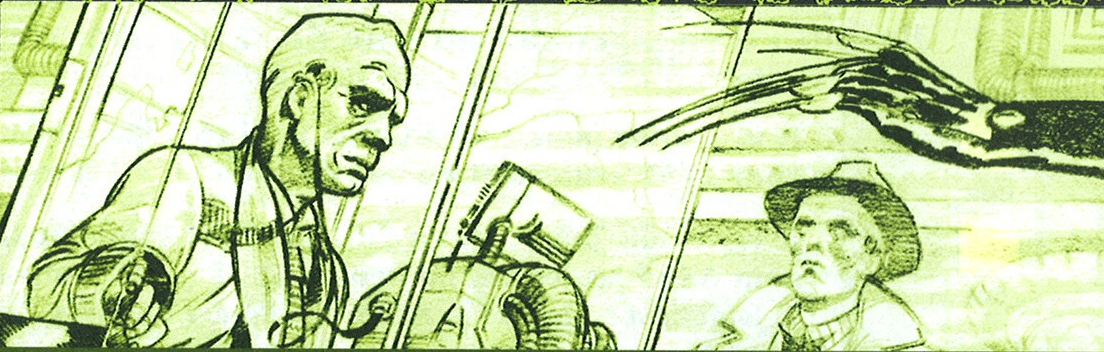
\includegraphics[width=0.48\textwidth]{img/MASTjohnRourkeMultivir.jpg}
	~\\ \emph{\footnotesize John Rourke faisant son briefing depuis une cabine Multivir\texttrademark } \end{center}

\vfill
\columnbreak

\textbf{\Large Secrets pas si secrets}~\\

Ces secrets sont les <<squelettes dans le placard>> de MediASsist. En travaillant quelques temps pour cette soci{\'e}t{\'e}, il est probable que les personnages tomberont dessus. Pour MediASsist ce serait m{\^e}me plut{\^o}t une preuve de leur comp{\'e}tence. La vraie question, celle qui va d{\'e}cider de leur vie future est: que faire de ces secrets ?
\begin{itemize}
	\item[$\bullet$] L'accident qui a co{\^u}t{\'e} la vie {\`a} Varron, l'un des fondateurs de l'entreprise, n'en {\'e}tait pas un. Il a {\'e}t{\'e} ex{\'e}cut{\'e} par les agents d'un \texttt{TechnoBloc} alors qu'il bouclait un dossier suffisant pour les exp{\'e}dier tous en prison pour quelques d{\'e}cennies. Le dossier a disparu, bien entendu. Les autres fondateurs consacrent pas mal de temps libre {\`a} essayer de le reconstituer. Lorsqu'ils auront termin{\'e}, ils le feront parvenir {\`a} un m{\'e}dia neutre... Bien ententu, ils se font parfois aider par certains de leurs employ{\'e}s. 
	\item[$\bullet$] Sans {\^e}tres ouvertement criminelles, certaines de leurs activit{\'e}s sont ill{\'e}gales. Il s'est trouv{\'e} un \texttt{TechnoBloc} pour avoir la patience d'accumuler un gros dossier sur toutes leurs irr{\'e}gularit{\'e}s. Il ne l'a pas encore utilis{\'e}, mais il pr{\'e}voit de s'en servir pour contraindre \mbox{MediASsist} {\`a} intervenir dans une op{\'e}ration contre un \texttt{TechnoBloc} rival qui est sur le point de d{\'e}velopper une \texttt{I.A.} viable. 
	\item[$\bullet$] Ogier intrigue beaucoup les rares curieux qui se sont pench{\'e}s sur ses origines. Pour l'instant personne ne semble avoir d{\'e}couvert la v{\'e}rit{\'e} : Ogier est une femme, et elle travaille pour l'\texttt{Acad{\'e}mie Dactyle}. Pourquoi les \texttt{Dactyles} se sont-ils donn{\'e}s la peine de cr{\'e}er MediASsist ? Sur les milliers de missions accomplies par la compagnie depuis dix-sept ans, combien ont {\'e}t{\'e} conduites sur ordre des Dactyles ? Lesquelles ? Et pourquoi ? Les autres fondateurs s'en doutent-ils ? En fait le vrai secret est {\`a} un niveau au-dessus : qui sont r{\'e}ellement les Dactyles ? Pour la plupart des gens, ils sont soit aussi folkloriques que des n{\'e}otempliers actuels, soit aussi (peu ?) influents que les francs-ma\c{c}ons.  
\end{itemize} %% ~\\

\textbf{\Large Mettre MediASsisT en <<jeu>>}~\\
MediASsist est un employeur id{\'e}al pour un groupe de personnages se conformant au sch{\'e}ma	cyberpunk standard du <<mercenaire sans scrupules>>. Mais il convient aussi assez bien aux personnages de \emph{Cyber Age}, qui ont g{\'e}n{\'e}ralement bonne r{\'e}putation, des contacts et des moyens un peu plus importants. L'entreprise est toujours {\`a} la recherche de nouveaux employ{\'e}s, ne r{\'e}pugne pas {\`a} sous-traiter certaines op{\'e}rations, paye confortablement... {\'E}videmment, en contrepartie, ses crit{\`e}res de qualit{\'e}s sont tr{\`e}s {\'e}lev{\'e}s. Les personnages ont int{\'e}r{\^e}t {\`a} {\^e}tre parfaitement efficaces s'ils veulent nouer des relations r{\'e}guli{\`e}res avec MediASsist. ~\\

\vfill
\columnbreak

\textbf{\large Techniquement}~\\
Les employ{\'e}s de MediASsisT se classent en quatre cat{\'e}gories (pour les personnages joueurs s'entend) : 
\begin{itemize}
	\item[$\bullet$] Les vacataires. Bien pay{\'e}s, on ne leur confie aucun mat{\'e}riel confidentiel, on les informe de ce qui peut mettre leur vie en danger, on n'enqu{\^e}te pas trop sur leur compte, on ne les <<arnaque>> pas. 
	\item[$\bullet$] Les grades Alpha. Correctement pay{\'e}s, ils ont toujours le dernier mat{\'e}riel technique de pointe. Les briefings sont aussi complets que ceux que l'on peut donner {\`a} des ex{\'e}cutants que l'on veut revoir en vie. On a fait une enqu{\^e}te normale sur leur compte. 
	\item[$\bullet$] Les grades B{\^e}ta. En plus du briefing, on leur explique ce que l'on croit savoir des buts recherch{\'e}s par le commanditaire (qui ne sont pas toujours ceux sp{\'e}cifi{\'e}s sur le contrat). En plus d'un paye tr{\`e}s honn{\^e}te, ils b{\'e}n{\'e}ficient d'un acc{\`e}s {\`a} des implants, c{\^a}blages et logiciels normalement accessibles seulement {\`a} des forces \texttt{Mercs} d'{\'e}lite. MediASsist a r{\'e}alis{\'e} sur leur compte une enqu{\^e}te plus qu'approfondie. Une personne qui aurait un pass{\'e} et un pr{\'e}sent vraiment trop flous ne pourrait pas acc{\'e}der au grade B{\^e}ta. MediASsist ne prend pas de risques {\`a} ce niveau l{\`a}. 
	\item[$\bullet$] Les actionnaires. En dehors des six actionnaires principaux, quelques employ{\'e}s poss{\`e}dent une partie de MediASsist en dehors de leur poste et salaire habituels. {\`A} vous de voir quels avantages et inconv{\'e}nients cela procure.  
\end{itemize}~\\

\barreCyberAgeHalf ~\\

\textbf{\large Entrer chez MediASsisT}~\\
\textbf{Vacataires} Rien de sp{\'e}cial n'est demand{\'e}, {\`a} part fournir la preuve d'un travail d{\'e}j{\`a} effectu{\'e} dans le domaine demand{\'e}. ~\\
\textbf{Grade Alpha} Quelques renseignements personnels sont demand{\'e}s. Il faut avoir fait une mission au moins en tant que vacataire, m{\^e}me si on ne l'a pas r{\'e}ussie. En {\'e}change, un stage gratuit permet de monter un talent technique au niveau +1, et un autre talent au niveau 0. ~\\
\textbf{Grade B{\^e}ta} Il faut avoir au moins r{\'e}ussi une mission en tant que grade Alpha, et accepter une enqu{\^e}te sur sa vie priv{\'e}e. Incidemment, un des <<secrets>> de \mbox{MediASsisT} sera r{\'e}v{\'e}l{\'e} au postulant. On {\'e}tudiera attentivement ce que la personne en fait. Une fois accept{\'e}, le personnage a le droit {\`a} un c{\^a}blage musculaire ou nerveux, ou {\`a} une broche de type C (au choix). Il suit un stage pour monter l'un des talents qu'il poss{\`e}de d{\'e}j{\`a} au niveau 0 ou +1 jusqu'au niveau +2. Lors de ce stage, il monte trois autres talents au niveau 0. ~\\

\barreCyberAgeHalf ~\\

\end{multicols}

\clearpage

\begin{multicols*}{3}

\section*{Les Dactyles\markboth{Les Dactyles}{Les Dactyles}}
\addcontentsline{toc}{section}{Les Dactyles}
\label{Dactyles}
\index{Dactyles@Dactyles, Les }
\index{AcademieDactyle@Acad{\'e}mie Dactyle, L'|see{Dactyles}}

\scriptsize{
Certaines rumeurs laissent entendre que l'acad{\'e}mie commen\c{c}a sa carri{\`e}re en tant qu'officine de tueurs {\`a} gages ou de terroristes, juste au lendemain de la Grande R{\'e}volution Lib{\'e}rale. C'{\'e}tait alors une secte qui professait l'assassinat politique, et qui tirait ses racines des anarchistes russes de la fin du XIXe si{\`e}cle. L'acad{\'e}mie fut donc au d{\'e}part une sorte d'{\'e}cole d'entra{\^i}nement pour commandos suicide. Mais tr{\`e}s vite, ses membres durent faire face {\`a} la dure concurrence des yakuzas et des tueurs des triades. Son Troisi{\`e}me Secr{\'e}tariat pris alors la d{\'e}cision de quitter la Terre pour les premi{\`e}res {\^I}les de la Lune. {\`A} l'{\'e}poque, c'{\'e}tait une d{\'e}cision tr{\`e}s aventureuse et tr{\`e}s co{\^u}teuse, mais l'acad{\'e}mie avait accumul{\'e} une jolie fortune gr{\^a}ce {\`a} ses assassinats politiques et les {\^I}les {\'e}taient le seul endroit o{\`u} les tueurs yakuzas n'iraient pas les suivre.~\\

Durant pr{\`e}s de quarante ans, on n'entendit plus parler de l'acad{\'e}mie. Les Iles de la Lune {\'e}taient encore un territoire pionnier, beaucoup de stations satellites disparaissaient, se regroupaient ou bien {\'e}taient d{\'e}mantel{\'e}es. Certaines structures d{\'e}riv{\`e}rent en Espace profond sans qu'on prenne la peine de faire des recherches ou d'essayer de sauver les colons qui pouvaient encore s'y trouver. C'{\'e}tait une {\'e}poque sans piti{\'e}. Dans les ann{\'e}es 2060, une rumeur commen\c{c}a {\`a} se r{\'e}pandre dans les services R{\'e}zo des grands \texttt{TechnoBlocs}, on parlait de certains \texttt{jackeurs}, particuli{\`e}rement dou{\'e}s, qui avaient tous un profil identique: ils avaient tous {\'e}t{\'e} form{\'e}s gratuitement dans une acad{\'e}mie des {\^I}les de la Lune. L'acad{\'e}mie Dactyle venait de refaire surface et bien s{\^u}r, personne ne fit le rapport avec la bande de n{\'e}oanarchistes russes qui s'{\'e}taient envol{\'e}s pour les {\'e}toiles quarante ans auparavant, et pourtant...~\\

\textbf{Infos semi-publiques}~\\

\textbf{Extrait d'un rapport sur la secte dites des <<Dactyles>> }~\\

Les Dactyles ont des r{\`e}gles tr{\`e}s strictes et tr{\`e}s {\'e}tranges : aucune ou tr{\`e}s peu de publicit{\'e}, interdiction de prononcer le nom de leurs membres, intervention la plus discr{\`e}te et la plus courte possible. On sait pourtant qu'ils recrutent des jeunes gar\c{c}ons ou filles, les forment {\`a} toutes les techniques du R{\'e}zo, et les renvoient dans la vie normale (sans contrepartie semble-t-il. Une fois ce qu'ils jugent comme {\'e}tant leur t{\^a}che accomplie les Dactyles disparaissent et g{\'e}n{\'e}ralement, le jeune gar\c{c}on ou la jeune fille qui a profit{\'e} de leur g{\'e}n{\'e}rosit{\'e} n'entendra plus jamais parler d'eux. Plusieurs rumeurs affirment qu'ils contr{\^o}lent {\'e}galement en sous main plusieurs {\'e}coles d'enseignement primaire et sup{\'e}rieur, mais aucun network n'a jamais pu en apporter une preuve formelle.~\\

Seules certitudes :
\begin{itemize}
	\item Les Dactyles sont divis{\'e}s en deux coll{\`e}ges non mixtes, la Main Gauche et la Main Droite. 
	\item Leur {\'e}tat major se trouve quelque part sur les {\^I}les de la Lune, ils disposent d'une fortune colossale d'une provenance inconnue et ma{\^i}trisent parfaitement les technologies informatiques.
\end{itemize}

\columnbreak

Comme les francs-ma\c{c}ons, les Dactyles peuvent se reconna{\^i}tre entre eux gr{\^a}ce {\`a} un syst{\`e}me complexe de signes de main et de doigts. Comme  les francs-ma\c{c}ons {\'e}galement, un Dactyle en danger peut esp{\'e}rer le secours de tout autre Dactyle gr{\^a}ce {\`a} un signe de d{\'e}tresse. C'est devenu une plaisanterie dans la \texttt{Matrice} que de rep{\'e}rer des <<signes Dactyles>>. Quand un message est incompr{\'e}hensible, ou qu'il porte une suite de cinq ou dix <<digits>> comme signature, on dit que c'est un message Dactyle.~\\

Ainsi le dicton : <<Les doigts de ta main droite sont tes Dactyles, et ceux de ta main gauche doivent {\^e}tre abandonn{\'e}s aux sorci{\`e}res>> semble ne rien vouloir dire. Bien entendu on a tout dit sur eux : qu'ils {\'e}taient des extraterrestres, des agents des \texttt{Sept Dragons}, des cyborgs... Mais personne aujourd'hui n'est encore capable de dire quels sont les buts de l'acad{\'e}mie Dactyles. Reste que la majorit{\'e} des grands \texttt{jackeurs} est issue de leurs rangs depuis pr{\`e}s de vingt ans.~\\

\textbf{Archiv{\'e} au CTI -- \texttt{MediASsisT} }~\\

\textbf{Mythologie}

Si l'on recherche dans les bases de donn{\'e}es au mot Dactyles on ne trouvera que des r{\'e}f{\'e}rences mythologiques, ce qui est un peu frustrant pour le pirate moderne.                                  
Les cinq Dactyles m{\^a}les {\'e}taient des forgerons, les cinq Dactyles femelles {\'e}taient des magiciennes. Leur origine est obscure. Il semblerait que Rh{\'e}a enceinte de Zeus, enfon\c{c}a ses doigts dans le sol pour soulager ses douleurs, et ainsi naquirent les Dactyles.~\\

Les Dactyles de la main droite sont des forgerons et des magiciens. ils travaillent le fer, et le fer fut dans l'antiquit{\'e} un m{\'e}tal sacr{\'e}. D'origine m{\'e}t{\'e}orique, {\`a} forte teneur en nickel, il ne rouillait presque jamais, c'est avec lui qu'on fabriquait les meilleures armes, il {\'e}tait bien entendu tr{\`e}s rare et la d{\'e}couverte d'une m{\'e}t{\'e}orite charg{\'e}e en fer {\'e}tait consid{\'e}r{\'e}e comme un pr{\'e}sent des dieux.~\\

Ce sont les Dactyles femmes qui enseign{\`e}rent les Myst{\`e}res de la Triple D{\'e}esse {\`a} Orph{\'e}e. On n'en sait pas plus.~\\

\textbf{Infos secr{\`e}tes}

La Main Gauche des Dactyles, qui se charge de l'enseignement des techniques de l'informatique est compos{\'e}e uniquement de femmes. Il n'y a pas de lieu propre {\`a} l'enseignement. Les <<sorci{\`e}res>>, comme elles se nomment parfois elles-m{\^e}mes, donnent des le\c{c}ons particuli{\`e}res ou montent des cours pour un temps donn{\'e}.~\\

Mais bien peu de gens connaissent l'autre face de l'acad{\'e}mie, il s'agit de l'activit{\'e} de la Main Droite ou la <<main masculine des Dactyles>>. En moins de cinquante ans elle s'est hiss{\'e} de fa\c{c}on tout {\`a} fait occulte au tout premier rang des fabricants d'armes l{\'e}g{\`e}res. Les ateliers secrets de l'acad{\'e}mie sont {\`a} l'heure actuelle capable de produire les meilleures armes l{\'e}g{\`e}res du monde et ce sans que le nom de l'acad{\'e}mie n'apparaisse une seule fois dans les rapports d'experts sur la production militaire mondiale.~\\

\columnbreak

Les armuriers de l'acad{\'e}mie vendent discr{\`e}tement leur production gr{\^a}ce {\`a} des interm{\'e}diaires et {\`a} des pr{\^e}tes noms. D'ordinaire ils vendent {\`a} tout le monde mais certaines commandes ne sont pas honor{\'e}es, les armuriers ne s'en expliquent jamais, si le client insiste, un contrat yakuza le ram{\`e}ne assez vite {\`a} la raison.~\\
 
Les armuriers de l'acad{\'e}mie ne font pas que fabriquer des armes, ils en inventent aussi, ils sont m{\^e}me {\`a} la pointe de la recherche dans plusieurs domaines, laser, armes molles, identification de cibles. Ils sont {\'e}galement tr{\`e}s sp{\'e}cialis{\'e}s dans les programmes d'attaques et de d{\'e}fense en cyberspace, notamment sur les mod{\`e}les de Glace de troisi{\`e}me g{\'e}n{\'e}ration, un type de Glace totalement reg{\'e}n{\'e}rable et virtuellement impossible {\`a} percer.~\\
 
Bien s{\^u}r, si on savait d'o{\`u} venaient les derni{\`e}res g{\'e}n{\'e}rations de Glace et de programmes tueurs depuis pr{\`e}s de dix ans, toutes les acad{\'e}mies seraient imm{\'e}diatement prise d'assaut par les forces des \texttt{TechnoBlocs} li{\'e}s {\`a} la vente d'armes, dans cette perspective on comprend mieux la discr{\'e}tion des secr{\'e}taires de l'acad{\'e}mie.~\\
 
Si on pouvait demander {\`a} un responsable de l'armurerie de l'Acad{\'e}mie la raison pour que cette derni{\`e}re ne fabrique que des armes l{\'e}g{\`e}res il aurait pourrait r{\'e}pondre quelque chose dans le genre <<Justement pour qu'on ne se serve que le moins possible des armes lourdes>>. Bien entendu les {\'e}normes profits de la Main Droite servent {\`a} financer les non moins {\'e}normes pertes de la Main Gauche.~\\

\textbf{Donn{\'e}es techniques}~\\

Les Dactyles sont environ une centaine (60 \% de femmes), dont la moiti{\'e} vit sur une base spatiale aux environs des lunes de Jupiter. Leur base proche est sur une des {\^I}les de la Lune. Ils poss{\`e}dent (sur Jupiter) un I.A.Q. de valeur 80, nomm{\'e}e Rh{\'e}a, sp{\'e}cialis{\'e}e dans la cr{\'e}ation de logiciels (Glaces et autres). Ce sont les Dactyles qui fournissent 60 \% des Glaces du R{\'e}zo, notamment les Glaces noires (60 \%).~\\

\textbf{Talents typiques d'une Dactyle} : Piratage +2, Informatique +2, Pratiques shamanique ou M{\'e}ditation zen +2, Enseignement +1, Com{\'e}die +1. Presque jamais de c{\^a}blage, sauf c{\^a}blage \texttt{Matrice} sp{\'e}cial (suivi d'une th{\'e}rapie pour remonter l'{\'E}quilibre psychique perdu).~\\

\textbf{Talents typiques d'un Dactyle} : Ing{\'e}nierie des armes +1, Armes l{\'e}g{\`e}res +1 ou 0, Commerce +1, Biologie/g{\'e}n{\'e}tique +1. En g{\'e}n{\'e}ral ils ont des c{\^a}blages divers interfac{\'e}s {\`a} des armes sp{\'e}ciales. 

\begin{center} \rule{4cm}{0.5mm} \end{center}

\texttt{\scriptsize{(Originellement Publi{\'e} dans : Casus Belli Hors s{\'e}rie n 16, Auteur : Pierre Rosenthal)}}

} % end scriptsize
\end{multicols*} 

\clearpage

\section*{CyberAge, CyberEspace et Matrice : La Plong{\'e}e\markboth{CyberAge, CyberEspace et Matrice : La Plong{\'e}e}{CyberAge, CyberEspace et Matrice : La Plong{\'e}e}}
\addcontentsline{toc}{section}{CyberAge, CyberEspace et Matrice : La Plong{\'e}e}
\label{PlongeeMatrice}
\label{JungleMatrice}
\label{KernelMatrice}
\index{Plong{\'e}e@CyberAge, CyberEspace et Matrice : La Plong{\'e}e}
\index{Plong{\'e}e@CyberAge, CyberEspace et Matrice : La Plong{\'e}e}
\index{Plong{\'e}e@Matrice, Plong{\'e}e}
\index{Plong{\'e}e  (Matrice)}
% \index{Jungle@Matrice|see{Plong{\'e}e  (Matrice)}}
% \index{Kernel@Matrice|see{Plong{\'e}e  (Matrice)}}
\index{Jungle (Matrice)|see{Plong{\'e}e  (Matrice)}}
\index{Kernel (Matrice)|see{Plong{\'e}e  (Matrice)}}

%% Univers Pour : 
\includegraphics[width=3cm]{../../../../../imgGraphics/rolePlayingGame/SimulacreS/logos/logoSimulacreS01.png}~\\

\begin{minipage}[ht]{0.45\textwidth}
% \textbf{\Large La plong{\'e}e}~\\
\textbf{\scriptsize Le R{\'e}zo, la Matrice, le cyberspace, tous ces mots d{\'e}signent la m{\^e}me chose tout en n'en montrant qu'une partie. Et quand des millions de connect{\'e}s partagent un m{\^e}me espace en croyant sinc{\`e}rement qu'il y a "quelque chose" derri{\`e}re tout \c{c}a, il est naturel -- alors que la technologie permet de manipuler les r{\^e}ves -- que ceux-ci se concr{\'e}tisent. }~\\

\texttt{\scriptsize{(Originellement Publi{\'e} dans : Casus Belli Hors s{\'e}rie n 16, Auteur : Pierre Rosenthal)}}
\end{minipage} \hfill \begin{minipage}[ht]{0.45\textwidth}
\colorbox{verylightgrey}{ \shadowbox{\scriptsize %
\begin{minipage}[ht]{0.90\textwidth}
\textbf{Glace Noire}~\\
Certaines Glaces peuvent d'un seul coup faire basculer un esprit dans le Kernel. Autant dire que pour quelqu'un de non pr{\'e}par{\'e}, c'est le choc traumatique assur{\'e}, d'o{\`u} les << l{\'e}gendes >> de \texttt{jackeurs} qui ont << br{\^u}l{\'e} >> leur cerveau.~\\
\textbf{Math{\'e}matiques chaotiques}~\\
Certains math{\'e}maticiens de tr{\`e}s haut niveau arrivent {\`a} aller dans le Kernel en utilisant le talent Math{\'e}matiques chaotiques {\`a} la place de celui de M{\'e}ditation Zen. Les diff{\'e}rences sont: pas de possibilit{\'e} de passer dans la Jungle; et le test de souvenir se fait sans le malus de -4 d{\`e}s que l'on veut des donn{\'e}es qui peuvent s'exprimer en mots ou en chiffres (pas plus de l'{\'e}quivalent d'une page de livre).~\\
\end{minipage} } }%
\end{minipage}

\begin{multicols}{3}
\scriptsize{

	\textbf{\Large La Jungle}~\\
	
	Dans l'encyclop{\'e}die, on vous a dit qu'il existait deux niveaux pour visiter le R{\'e}zo : \texttt{HyperNet} et la \texttt{Matrice}. En fait, il existe encore deux autres niveaux que peu de \texttt{jackeurs} connaissent, m{\^e}me si les termes qui les d{\'e}finissent leur sont familiers.~\\
	
	Tout d'abord, au niveau inf{\'e}rieur {\`a} la \texttt{Matrice}, il y a un niveau que nous d{\'e}signerons sous le nom de Jungle (parfois connu sous le nom de Grand Bleu -- d'o{\`u} le terme de plong{\'e}e, ou Reptilien, ou Jurassique). Ce niveau correspond {\`a} celui que nous appelons dans nos ordinateurs actuels : syst{\`e}me d'exploitation. Dans les ann{\'e}es 2080, on ne programme quasiment plus en code. On donne des instructions symboliques. Et les syst{\`e}mes communiquent entre eux par des techniques d'HDI (Holographic Dreams Image, IRH en fran\c{c}ais). Ces flots d'HDI sont des donn{\'e}es extr{\^e}mement compactes -- cod{\'e}es comme des images fractales, de m{\^e}me type que celles produites par les machines {\`a} r{\^e}ves. Ils permettent de faire circuler en m{\^e}me temps des donn{\'e}es, des instructions et des configurations (nouvelle fa\c{c}on d'appr{\'e}hender les donn{\'e}es). Au XXI' si{\`e}cle (en faisant un raccourci), on peut dire que les ordinateurs communiquent entre eux en r{\^e}vant, ou en s'{\'e}changeant des r{\^e}ves.~\\
	
	\textbf{\large Ce qui se passe dans la Jungle}~\\
	
	Dans la Jungle, le \texttt{jackeur} se verra comme il s'imagine en r{\^e}ve. Il n'y aura plus de Glaces, de \texttt{TechnoBlocs}, de zones de donn{\'e}es. Si le \texttt{jackeur} s'imagine comme un chevalier, il sera recouvert d'une armure brillante, chevauchant peut-{\^e}tre dans une verte plaine. Tant que le \texttt{jackeur} navigue dans des zones visit{\'e}es par tout le monde, c'est sa vision qui s'impose. Quand il approche d'un \texttt{TechnoBloc}, c'est l'image inconsciente de la structure qui s'impose. En g{\'e}n{\'e}ral on rencontrera un gigantesque robot, un comptable retors, etc. Mais il faut bien dire que nombre de \texttt{TechnoBlocs} se voient comme de redoutables pr{\'e}dateurs, et les \texttt{Sept Dragons} n'ont pas vol{\'e} leur nom.~\\
	
	Si on veut << voler >> une donn{\'e}e au \texttt{TechnoBloc}, il faudra le vaincre. Ce qui peut {\^e}tre tr{\`e}s dangereux. On peut aussi, ce qui est impossible dans la \texttt{Matrice}, dialoguer avec le syst{\`e}me d'un \texttt{TechnoBloc}, le persuader, le charmer, lui demander des renseignements. Et peut-{\^e}tre r{\'e}ussir. Une fois sorti de la Jungle, dans la \texttt{Matrice}, on retrouvera les informations donn{\'e}es ou vol{\'e}es dans sa m{\'e}moire informatique comme si on venait de les pirater.~\\
	
	\textbf{\Large Le Kernel}~\\
	
	Une Intelligence Artificielle est une cr{\'e}ature du R{\'e}zo, et aucun humain ne peut penser un jour l'{\'e}galer en habilit{\'e} et en vitesse (une I.A. fait cent mille millions de milliards de fois plus d'op{\'e}rations simultan{\'e}es qu'un humain). Mais c'{\'e}tait compter sans l'astuce et la philosophie de certains moines \texttt{jackeurs} tib{\'e}tains, qui d{\'e}velopp{\`e}rent la technique de << plong{\'e}e profonde >>, dite << petit nirvana >>. Puisque les ordinateurs communiquent par une certaine forme de pens{\'e}e, il suffisait de rendre son esprit proche de ce m{\^e}me mode, devenir un relais, une m{\'e}moire pour le R{\'e}zo, dispara{\^i}tre pour se fondre dans la \texttt{Matrice}. Il ne reste alors plus qu'{\`a} << d{\'e}river >> dans le Kernel (le niveau inf{\'e}rieur {\`a} la Jungle, celui o{\`u} les flots HDI naviguent de fa\c{c}on r{\'e}flexe, sans plus aucune volont{\'e} consciente) jusqu'aux abords du lieu que l'on veut conna{\^i}tre. Le syst{\`e}me informatique utilisera alors le cerveau du \texttt{jackeur} comme relais, s'appropriant ses synapses. Une fois la transe termin{\'e}e, le \texttt{jackeur} n'a alors plus qu'{\`a} se << souvenir >>, les donn{\'e}es qu'il cherche sont quelque part dans sa m{\'e}moire.~\\
	
	\textbf{\large Les dangers du Kernel}~\\
	
	Le probl{\`e}me d'ouvrir son cerveau aux ordinateurs est que l'on ouvre la porte {\`a} toutes les manipulations. Tout d'abord, si son esprit n'est pas assez vide (il ne faut plus penser {\`a} rien qu'a objectif) les logiciels sentent une r{\'e}sistance et br{\^u}lent litt{\'e}ralement le cerveau. Ensuite il faut savoir verrouiller des parties de son cerveau, sinon on se r{\'e}veille en ayant perdu toute sa m{\'e}moire, et parfois pire encore (se souvenir que 3 plus 18 font 1, et que la soude caustique se d{\'e}guste {\`a} temp{\'e}rature ambiante, est assez handicapant). Enfin, il faut arriver {\`a} se souvenir de donn{\'e}es qui auront peut-{\^e}tre {\'e}t{\'e} rang{\'e}e tr{\`e}s loin dans sa m{\'e}moire. Il n'est pas rare qu'un \texttt{jackeur} tib{\'e}tain de 60 ans, apr{\`e}s une visite au Kernel, se "souvienne" avoir inscrit un code sur un papier quand il avait 12 ans. Mais ce code {\'e}tait-il C2A4S6 ou C3A46S ? Le souvenir remonte quand m{\^e}me {\`a} 48 ans dans le pass{\'e} pour le moine.~\\
	
	\textbf{\Large En jeu}~\\
	
	\textbf{\large Entrer dans la Jungle/Kernel}~\\
	
	Il faut d'abord {\^e}tre dans la \texttt{Matrice}. Puis faire un test de mise en transe. Un \texttt{jackeur} qui ne sait pas que la Jungle et le Kernel existent n'aura pas cette id{\'e}e de lui m{\^e}me. Le test vaut Esprit~\imgESPRI + D{\'e}sir~\imgDESIR + Humain~\imgHUMAI + [M{\'e}ditation Zen] -4. La M{\'e}ditation Zen est un talent qui est une technique sp{\'e}cialis{\'e}e avec une base de -4. Si le test {\'e}choue, on subit une d{\'e}connexion brutale (perte de 3PS). Si on r{\'e}ussit, la Marge de R{\'e}ussite indique jusqu'o{\`u} on peut descendre.~\\
	\textbf{Marge de 1 {\`a} 3} : on reste {\`a} la frange, sans pouvoir descendre dans la Jungle.~\\
	\textbf{Marge de 4 {\`a} 16} : Jungle. ~\\
	\textbf{Marge de 17 {\`a} 20} : on est entre Jungle et Kernel, cela permet {\`a} ceux qui ne connaissent que la Jungle de savoir qu'il y a quelque chose dessous.~\\
	\textbf{Marge de 21 et plus} : Kernel.~\\
	
	\textbf{\large {\^E}tre et agir dans la Jungle}~\\
	
	Agir dans la Jungle est tout simplement jouer {\`a} un jeu de r{\^o}le dans le jeu de r{\^o}le. C'est au meneur de jeu de trouver des adversaires, des pi{\`e}ges, des qu{\^e}tes {\`a} accomplir pour avoir les renseignements. Tous les talents sont conserv{\'e}s par le personnage en Jungle. II n'a plus d'{\'e}quipement autre que le mat{\'e}riel standard correspondant {\`a} l'univers o{\`u} il {\'e}volue. On {\'e}change ses valeurs de Corps et Instincts pour tous les tests qu'il a {\`a} faire. De plus un malus affecte tous ses tests d{\`e}s qu'il va << loin >> (sur une autre grille, une autre SatZone). Un personnage qui perd tous ses PS ou tous ses PV est {\'e}ject{\'e} de la Jungle. Quand on perd des PV, ils sont convertis en EP {\`a} la sortie de la Jungle. Pour sortir volontairement de la Jungle, il faut r{\'e}ussir un test Esprit~\imgESPRI + Action~\imgACTIO + Humain~\imgHUMAI + [M{\'e}ditation Zen]. En cas d'{\'e}chec, il y a d{\'e}connexion brutale.~\\
	
	\textbf{\large {\^E}tre et agir dans le Kernel}~\\
	
	Dans le Kernel il faut d'abord ne pas {\^e}tre, donc r{\'e}ussir un test Esprit~\imgESPRI + R{\'e}sistance~\imgRESIS + N{\'e}ant~\imgNEANT + [M{\'e}ditation Zen] (le N{\'e}ant vaut -1). En cas d'{\'e}chec, on subit [B] EP et on est d{\'e}connect{\'e}. Ensuite il faut se laisser d{\'e}river dans le Kernel jusqu'{\`a} son objectif, test Esprit~\imgESPRI + D{\'e}sir~\imgDESIR + M{\'e}canique~\imgMECAN + [M{\'e}ditation Zen]. Si on {\'e}choue, un programme passe dans une partie du cerveau et le br{\^u}le, faisant [B]PV de d{\'e}g{\^a}ts d{\'e}finitifs sur une partie du corps. Il faut ensuite savoir quand remonter, et faire un test Esprit~\imgESPRI + Perception~\imgPERCE + M{\'e}canique~\imgMECAN + [M{\'e}ditation Zen]. Si ce test {\'e}choue, aucune autre cons{\'e}quence que celle de ne pas avoir r{\'e}ussi. Enfin, il faut se souvenir de ce que l'on a {\'e}t{\'e} chercher, avec un test Esprit~\imgESPRI + Action~\imgACTIO + Humain~\imgHUMAI + [M{\'e}ditation Zen] -4. Si le test {\'e}choue, on n'aura que des souvenirs fragmentaires. Le gros avantage du Kernel est que l'on n'y rencontre plus ni Glace ni I.A. Le gros d{\'e}faut : on met son cerveau en gage {\`a} chaque fois.~\\
} % end scriptsize
\end{multicols} 

\clearpage



\begin{multicols}{2}

\section*{Magie, Matrice et I.A.C.\markboth{Magie, Matrice et I.A.C.}{Magie, Matrice et I.A.C.}}
\addcontentsline{toc}{section}{Magie, Matrice et I.A.C.}
\label{MagieMatriceIAC}
\index{Magie@Magie, Matrice et I.A.C.}

{\footnotesize
	
	\textbf{\Large De la Th{\'e}orie}
	
	Il existe une th{\'e}orie expliquant que la magie a exist{\'e} sur notre plan{\`e}te, il y a tr{\`e}s tr{\`e}s longtemps. En ces temps-l{\`a}, certaines formes de vie utilisaient les <<fluides>> magiques pour modeler le monde autour d'elle. Cette {\'e}nergie magique a la particularit{\'e} de na pas pouvoir coexister avec le fer, et tout ce qui contient cetv {\'e}l{\'e}ment. Les premiers hommes qui fa\c{c}onn{\`e}rent le fer m{\'e}t{\'e}oritique venu des {\'e}toiles purent lutter contre ces formes de vie, leur plantant des pieux de fer en plein corps. Les hommes apprirent aussi la magie, car elle {\'e}tait facile {\`a} cette {\'e}poque. Mais {\'e}tant eux-m{\^e}me compos{\'e} avec du sang, et donc du fer, leur magie fut moins pure, plus destructrice que cr{\'e}atrice. En effet, le contact du fer et de la magie provoque chaleur et chaos. Trop de fer d{\'e}truit la magie, trop de magie fait fondre le fer. ~\\
	
	Au temps d'Ulysse et d'Hom{\`e}re, au temps des Pharaons les magiciens {\'e}taient encore puissants sur le Vieux Continent, et des cr{\'e}atures magiques encore visibles parmi les hommes. --- Lors de la d{\'e}couverte des Am{\'e}riques, l'Europe {\'e}tait devenue suffisamment <<industrialis{\'e}e>> pour que la maie y ait disparu. Les Incas la ma{\^i}trisait encore mais ils furent d{\'e}truits par les arm{\'e}es de fer de l'Espagne. Les fluides magiques {\'e}taient encore vivaces dans les Cara{\"i}bes, les esclaves noirs y apport{\`e}rent leurs pratiques vaudoues. On pouvait encore {\'e}galement pratiquer la magie aux Am{\'e}riques, ansi qu'en Afrique, au fond du Tibet, en Australie. ~\\
	
	Au XX\up{{\`e}me} si{\`e}cle, plus de magie, plus de cr{\'e}atures fantastiques. Il ne nous resta que des l{\'e}gendes des illumin{\'e}s New Age et des mystificateurs. Comment en effet croire, m{\^e}me aux Temps Antiques, que l'on puisse tordre une cuill{\`e}re <<en fer>>. --- Au XXI\up{{\`e}me}, la magie n'est pas plus pr{\'e}sente. La seule diff{\'e}rence c'est que certains ethnologues se sont rendus compte que des shamanes disant pratiquer la magie peuvent en effet produire {\`a} distance proche des effets de d{\'e}placement d{\'e}tectable au niveau des {\'e}lectrons. ~\\
	
	D'o{\`u} l'id{\'e}e que la magie n'a pas disparu. Elle est seulement sous une chape de plomb telle que l'on ne peut plus mesurer de fa\c{c}on visible son pouvoir. Toutes proportions gard{\'e}es, la puissance de la magie en 2080 est {\'e}quivalente {\`a} celle qu'a une pinc{\'e}e de sel sur un cyclone ! ~\\
	
	Mais en 2080, il y a un domaine o{\`u} le fait de changer quelques {\'e}lectrons de place peut s'av{\'e}rer primordial : la micro{\'e}lectronique et l'informatique. Heureusement pour nos braves <<magiciens>>, les mat{\'e}riels de haut de gamme ne contiennent que des mat{\'e}riaux composites {\`a} base de carbone, des liaisons en or ou en argent, des structures cristallines non m{\'e}talliques, et des liaisons optique laser. Voici pour la th{\'e}orie, passons {\`a} la pratique. ~\\
	
	\footnotesize{\textbf{Bibliographie. } Livres : \emph{les voies d'Anubis}, \emph{Sur des mers plus ignor{\'e}es} et \emph{Le poid de son regard} de Tim Powers, J'ai Lu. Jeux : \emph{SangDragon}, Casus Belli et \emph{Capitaine Vaudou}, Descartes {\'E}diteur. } ~\\
	
	\barreCyberAgeHalf ~\\
	%% \vfill
	%% \columnbreak
	
	\textbf{\Large Les bases de la Magie} ~\\
	\textbf{\large Les pr{\'e}requis} ~\\
	\textbf{\footnotesize Pour pratiquer la magie, il faut avoir deux choses : } %% ~\\
	\begin{itemize}
		\item[$\bullet$] Un ou plusieurs points dans une {\'E}nergie magique (vaudou, cabale, r{\^e}ves aborig{\`e}nes, etc.). Cette {\'E}nergie repr{\'e}sente le dergr{\'e} de croyance v{\'e}ritable et d'affinit{\'e} que l'on a avec ce type de magie. %% On peut mettre des points dans cette {\'E}nergie {\`a} la cr{\'e}ation du personnage, ou plus tard en d{\'e}pensant des PA. 
		\item[$\bullet$] La pratique des rituels magiques, que l'on a appel{\'e} de fa\c{c}on g{\'e}n{\'e}rique pratiques shamaniques mais qui varie pour chaque magie (pratiques vaudous, spiritisme, etc.). %% C'est un talent qui a une base de -4. 
	\end{itemize} ~\\
	\textbf{\footnotesize Il ne faut pas : } %% ~\\
	\begin{itemize}
		\item[$\bullet$] Avoir du fer (ou acier) sur soi. Ceci interdit la plupart des c{\^a}blages normaux, qui ont tous des composites avec des traces de fer ou des m{\'e}taux ferreux. la plupart des broches emp{\^e}chent aussi la magie, sauf certaines broches d'interface Matrice haut de gamme.   
		\item[$\bullet$] Avoir mang{\'e} la chair d'un animal {\`a} h{\'e}moglobine (ayant du sang rouge, donc {\`a} haute teneur en fer) depuis moins de six (6) heures. 
		\item[$\bullet$] Avoir plus de 500g de fer {\`a} moins de trois m{\`e}tres de soi. 
	\end{itemize} ~\\
	\small
	\textbf{\large La transe} ~\\
	La pratique de la magie ne se fait jamais de fa\c{c}on consciente. Elle plonge le <<magicien>> dans une transe, un r{\^e}ve, un d{\'e}lire mystique. Lors de cette transe, il a des visions, des r{\^e}ves, qu'il doit interpr{\'e}ter, dans lesquels il {\'e}volue parfois. ~\\
	
	Pour se mettre en {\'e}tat de transe il faut d{\'e}penser 1 EP, avoir au moins 1 point d'{\'E}nergie magique, se pr{\'e}parer {\`a} la transe par les rituels appropri{\'e}s (entre 30 minutes et 2 heures de temps), et r{\'e}ussir un test Instincts~\imgINSTI + D{\'e}sir\imgDESIR + Animal~\imgANIMA + Pratique shamanique -4 ~\\
	
	%% C'est le meneur de jeu, en fonction de la Marge de r{\'e}ussite, du sc{\'e}nario, et de la demande du magicien, qui en inventera les effets. ~\\
	
	\textbf{\large Les effets}~\\
	La magie n'aura jamais aucun effet direct dans le monde <<normal>>. Et il sera <<limit{\'e}>> dans l'univers virtuel du Rezo. Le probl{\`e}me de la notion de <<limite>> est que c'est la m{\^e}me que celle qui r{\'e}git les souhaits ou les f{\'e}es dans les contes merveilleux. On ne peut faire qu'une chose par acte magique, mais la difficult{\'e} suppos{\'e}e de l'acte n'a strictement rien {\`a} voir avec l'id{\'e}e que l'on Peut s'en faire. ~\\
	\textbf{Exemples d'actes magiques simples : } d{\'e}clencher un tir d'armes laser satellite sur une ville (c'est simple il suffit de <<pousser un bouton>>), avoir le code d'entr{\'e}e d'un syst{\`e}me informatique (on va {\`a} l'entr{\'e}e et on demande poliment). ~\\
	\textbf{Exemples d'actes magiques tr{\`e}s compliqu{\'e}s : } Diminuer ou augmenter son compte en banque (c'est tr{\`e}s long de recompter cet argent un {\`a} un), retrouver quelqu'un (il faut demander partout, \c{c}a prend du temps), recopier un gros fichier informatique (les esprits magiques n'ont pas que \c{c}a {\`a} faire). ~\\ 
	
	%% \barreCyberAgeHalf
	%% \vfill
	%% \columnbreak
	
	\textbf{\Large Divers types de magie}~\\
	\textbf{\large Le vaudou}~\\
	C'est la magie la plus pratiqu{\'e}e par les \texttt{Jackeurs}. On la pratique soit avant une passe informatique, pour augmenter ses chances, soit {\`a} c{\^o}t{\'e} d'un autre jackeur que l'on va ainsi aider. Certains <<technoshamanes>> sont capables de se mettre en transe dans la Matrice pendant une passe (il faut au moins une {\'E}nergie vaudou de 2, et d{\'e}penser 2 EP). ~\\
	
	Le pratiquant vaudou passe toujours par l'appel {\`a} des loas, sortes de deux-esprits. On ne voit les loas qu'en r{\^e}ves, ou dans la Matrice si on s'y met en transe. Ils adorent donner leurs indications par voies de r{\^e}ves cryptiques, de phrases sibyllines. Les pr{\^e}tres vaudou insistent sur le fait  qu'il faut toujours payer un loa qui vous a aid{\'e}. La fa\c{c}on de payer est diff{\'e}rente pour chaque loa. La plupart des d{\'e}tracteurs disent que cela prouve que le vaudou est une fumisterie destin{\'e}e {\`a} enrichir des imposteurs. Mais les shamanes connaissent des tas d'histoires o{\`u} des jackeurs qui ont oubli{\'e} de de payer ont trouv{\'e} la mort dans des circonstances particuli{\`e}rement {\'e}tranges. Les dix loas les plus connus, et les plus efficaces (parait-il) suivent. Les pouvoirs sont ceux qui leur sont le plus souvent attribu{\'e}s. ~\\ 
	
	\footnotesize	
	\textbf{\underline{La m{\`e}re des technoloas}}~\\ %%%%%
	$\bullet$ \textbf{Dame Gina (Gardienne du Rezo)}~\\
	\textbf{Pouvoir : }augmente les chances du jackeur (bonus de +1 ou +2, NAS +1 ou +2) durant une passe. ~\\ 
	\textbf{Paiement : }donner, dans les 24 heures qui ont suivi la passe, un Brise-Glace efficace {\`a} un jackeur inconnu dans la Matrice. ~\\
	
	\textbf{\underline{Les sept loas sup{\'e}rieurs}}~\\ %%%%%
	$\bullet$ \textbf{Papa Legba (Ma{\^i}tre Carrefour, ma{\^i}tre des chemins)}~\\
	\textbf{Pouvoir : }interc{\`e}de aupr{\`e}s des autres loas, permet de trouver plus rapidement un fichier dans une base de donn{\'e}es, permet de faire une passe dans une SatZone voisine comme si on {\'e}tait dans une grille voisine. ~\\ 
	\textbf{Paiement : }faire transiter plusieurs m{\'e}gaoctets de nouvelles donn{\'e}es d'une mn{\'e}mobase {\`a} une autre, dans les 24 heures suivantes. ~\\
	$\bullet$ \textbf{Loco (Docteur feuille)}~\\
	\textbf{Pouvoir : } prot{\`e}ge le jackeur contre certains d{\'e}g{\^a}ts dans la Matrice, emp{\^e}che l'usage du vaudou contre soi. ~\\ 
	\textbf{Paiement : } verser 1000~\euro ~{\`a} n'importe quelle Organisation d'Aide Non TechnoBloc. ~\\
	$\bullet$ \textbf{Ogou (Dieu de la guerre)}~\\
	\textbf{Pouvoir : } augmente le Potentiel d'Attaque de tous ses logiciels (d'une ou deux colonnes), pendant une passe enti{\`e}re. ~\\ 
	\textbf{Paiement : } acheter une arme l{\'e}g{\`e}re neuve, s'engager gratuitement dans une guerre priv{\'e}e. ~\\
	$\bullet$ \textbf{Damballah Vedo (dieu de la fortune et du commerce)}~\\
	\textbf{Pouvoir : } bonus de +4 {\`a} toute tentative de connaissance d'un mouvement d'argent. ~\\ 
	\textbf{Paiement : } verser au moins 10\% (minimum de 500~\euro ) de ce que la connaissance des mouvements de fonds a permis de gagner {\`a} un compte sp{\'e}cial. Ce compte est n'importe quel compte situ{\'e} dans les Cara{\"i}bes qui commence par les deux lettres DV. Il est fortement d{\'e}conseill{\'e} {\`a} quiconque de se cr{\'e}er ce genre de compte. Les sommes qu'on y d{\'e}pose ont tendance {\`a} <<s'{\'e}vaporer>>. ~\\
	$\bullet$ \textbf{Erzulie (d{\'e}esse de l'amour)}~\\
	\textbf{Pouvoir : } permet de se cr{\'e}er des personnalit{\'e}s particuli{\`e}rment r{\'e}ussies dans les univers virtuels divers (Synthivers et autres) ; peut modifier {\`a} distance (mais toujours par le Rezo) des puces d'Onirogrammes. ~\\ 
	\textbf{Paiement : } donner des informations secr{\`e}tes {\`a} un Network. ~\\
	$\bullet$ \textbf{Marinette (d{\'e}esse des zombie et des loups-garous)}~\\
	\textbf{Pouvoir : } permet de transporter sur soi un programme tueur difficilement d{\'e}tectable, peut modifier {\`a} distance (mais toujours par le Rezo) des puces d'Onirogrammes. ~\\ 
	\textbf{Paiement : } s'inscrire {\`a} une \texttt{Chasse}. ~\\
	$\bullet$ \textbf{Agoue (dieu de la mer, des temp{\^e}tes)}~\\
	\textbf{Pouvoir : } permet d'acc{\'e}der {\`a} des syst{\`e}mes que l'on croirait isol{\'e}s, pourvu que ceux-ci aient physiquement {\`a} port{\'e}e des syst{\`e}mes de transmission par radio, infrarouge et micro-onde. ~\\ 
	\textbf{Paiement : } verser 1000~\euro ~{\`a} une fondation pour les {\'e}tudes climatologiques. ~\\
	
	\textbf{\underline{Les deux loas inf{\'e}rieurs}}~\\ %%%%%
	$\bullet$ \textbf{Baron Samedi}~\\
	\textbf{Pouvoir : } permet de ressentir de fa\c{c}on plus r{\'e}aliste un passage en Synthivers. ~\\ 
	\textbf{Paiement : } jouer au moins 100~\euro ~dans un casino le samedi suivant. ~\\
	$\bullet$ \textbf{Gu{\'e}d{\'e} les trois}~\\
	\textbf{Pouvoir : } permet de trouver rapidement une adresse pour se procurer de la drogue. ~\\ 
	\textbf{Paiement : } aller voir un spectacle {\`a} un D{\^o}me quelconque. ~\\
	
	\vfill
	\columnbreak
	
	\small
	\textbf{\large Les r{\^e}ves australiens}~\\
	Les aborig{\`e}nes australiens pensent qu'il existe une sorte d'univers concomitant au notre, o{\`u} le temps n'a pas la m{\^e}me valeur que dans notre monde, et auquel on acc{\`e}de par les r{\^e}ves. ~\\
	Pendant une transe hors de la Matrice, le shamane se verra dans un monde r{\^e}v{\'e} et fantastique lutter contre des cr{\'e}atures magiques. S'il r{\'e}ussit {\`a} vaincre ses ennemis, un <<signe>>, lui appara{\^i}tra, lui indiquant ce qu'il voulait savoir, un peu comme les r{\^e}ves vaudou. ~\\
	%% Ce monde r{\^e}v{\'e} est tr{\`e}s proche de celui du <<Pays des r{\^e}ves>> d{\'e}crit dans le dernier sc{\'e}nario de ce hors-s{\'e}rie. Les r{\^e}gles pour y agir sont {\`a} la page~\pageref{}. ~\\
	Passer en transe dans la Matrice fait directement tomber au niveau Jungle -- Il faut avoir deux (2) points en {\'E}nergie Onirique. On n'a pas {\`a} payer quoi que ce soit pour aller dans le Pays des R{\^e}ves. Il faut par contre avoir au moins un (1) point en {\'E}nergie Onirique. ~\\ 
	
	\textbf{\Large Le point de vue du scientifique}~\\
	Pour Henri Shmier, scientifique de haut niveau, qui a {\'e}tudi{\'e} tous ces ph{\'e}nom{\`e}nes, la magie c'est de la foutaise. Il indique qu'il n'a jamais pu mesurer la moindre variation de champs magn{\'e}tique aupr{\`e}s des shamanes. Sa th{\'e}orie est bien plus simple : ~\\
	--- \emph{Il existe au moins sept Intelligences Artificielles Conscientes dans le Rezo, et ce sont les Sept Dragons qui les contr{\^o}lent ({\`a} moins que ce ne soit le contraire). Pour une Intelligence Artificielle de ce niveau, et avec les technologies modernes des lampes {\`a} r{\^e}ves, des onirogrammes et des Synthivers, il est tout {\`a} fait possible de s'incarner dans des mondes virtuels ainsi que dans les r{\^e}ves de gens. } ~\\
	\emph{Quant aux pouvoirs pr{\'e}sum{\'e}s des magiciens, il n'y a rien qu'une Intelligence Artificielle d{\'e}termin{\'e}e ne puisse arriver {\`a} faire. De plus, cette habitude de paiement suite aux actes magiques semble bien favoriser plut{\^o}t les Sept Dragons. En fait, la magie n'est qu'un {\'e}cran, une tentative de masquer sous la superstition le fait que nos vies sont maintenant soumises {\`a} la volont{\'e} d'entit{\'e}s non humaines : les Intelligences Artificielles Conscientes. Qui ont de plus cr{\'e}{\'e} une police des polices : les unit{\'e}s Cr{\'e}puscules, pour {\'e}viter que d'autres Intelligences viennent se partager le g{\^a}teau !}~\\
	Hector Shmier est un invit{\'e} r{\'e}gulier de shows t{\'e}l{\'e}vis{\'e}s. Il a une apparence un peu ridicule et un l{\'e}ger z{\'e}zaiement. Quand on le connait et qu'on lui demande qui lui a donn{\'e} l'id{\'e}e de cette th{\'e}orie, il avoue qu'elle lui est arriv{\'e}e un beau matin, par courrier {\'e}lectronique. ~\\
			
	\textbf{\Large Une information suppl{\'e}mentaire}~\\
	Il existe en effet neuf Intelligences Artificielles Conscientes (\texttt{I.A.C.}) r{\'e}pertori{\'e}es dans le \texttt{Rezo}. Ce sont celles des \texttt{Sept Dragons}, du \texttt{yakuza} et des \texttt{triades}. Le \texttt{califat de Carthage} a une I.A. qui pourrait devenir consciente si les autres I.A. lui ouvrait un acc{\`e}s plus grand au Rezo (ce qu'elles ne veulent pas). On sait que les Dactyles ont une \texttt{I.A.Q.} mais pr{\`e}s de Jupiter. Elle ne peut donc quasiment pas acc{\'e}der au Rezo. Toutes ces informations peuvent valoir l'{\'e}limination imm{\'e}diate {\`a} qui tente de les diffuser de fa\c{c}on r{\'e}ellement convaincante. ~\\
	
	Il n'existe aucune preuve r{\'e}elle d'une dixi{\`e}me I.A.C. sur le Rezo, et personne ne semble en contr{\^o}ler une autre. Mais certains ph{\'e}nom{\`e}nes dy cyberespace s'expliqueraient bien mieux si : 
	\begin{itemize}
		\item[$\bullet$] Il y avait une 10\up{{\`e}me} I.A.C. et <<libre>> sur le Rezo ; 
		\item[$\bullet$] La magie existait.
	\end{itemize} 
	
} % \footnotesize
\end{multicols}

\clearpage

\begin{multicols*}{3}

\section*{Annabella Grubert, ~\\ cyber psychiatre\markboth{Annabella Grubert, cyber psychiatre}{Annabella Grubert, cyber psychiatre}}
\addcontentsline{toc}{section}{Annabella Grubert, cyber psychiatre}
\label{AnnabellaGrubert}
\index{AnnabellaGrubert@Annabella Grubert, cyber psychiatre}

\textbf{\textit{\small Dans l'univers impitoyable CyberPunk, les \texttt{jackeurs} (pirates ou inconscients d{\'e}r{\'e}gulateurs du syst{\`e}me) mettent leur cerveau en jeu pour aller chercher le saint graal du futur -- l'information. Malheureusement nombreux sont ceux qui se grillent les neurones au contact des glaces noires noires. Une fois la passe destructrice effectu{\'e}e, sont-ils vraiment irr{\'e}cup{\'e}rables ?}}~\\
\texttt{\scriptsize{(\textbf{Le petit capharna{\"u}m} n 22 --- Texte : \textbf{Pierre Rosenthal} / Illustration : \textbf{{\'E}ric Puech)} }}

\begin{center} 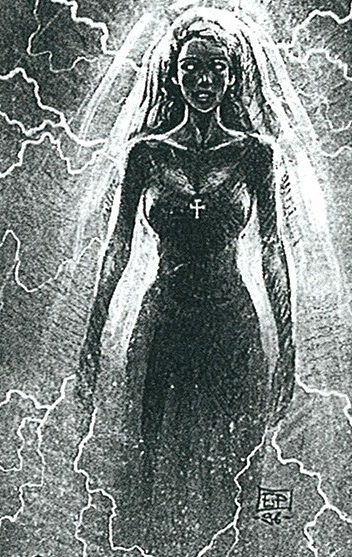
\includegraphics[width=0.30\textwidth]{img/AnabellaGrubertCyberPsychiatre.jpg} \end{center}

{\footnotesize 

	\textbf{\Large Refus d'existence}~\\
	
	Que les pirates informatiques existent, personne n'en disconvient. Qu'ils s'appellent \texttt{jackeurs}, deckers, runners, cowboys, \c{c}a aussi tout le monde le sait. Mais que les \texttt{TechnoBlocs} (et autres m{\'e}gacorps) utilisent sciemment des programmes de d{\'e}fense qui bousillent le cerveau des intrus, c'est plus discutable. Non pas que ce soit un secret, mais c'est plut{\^o}t un fait indiscut{\'e} pour lequel il n'y a pas vraiment de preuves. Apr{\`e}s tout, ceux qui ont rencontr{\'e} une glace noire sont rarement en {\'e}tat d'en parler.~\\
	
	\vfill
	\columnbreak
	
	\textbf{\Large L'Institut du ~\\ Bon Secours}~\\
	
	Que faire alors de ces l{\'e}gumes vivants, surtout s'ils n'ont pas pay{\'e} leurs cotisations sociales. Annabella Grubert a trouv{\'e} une solution. Ag{\'e}e d'une trentaine d'ann{\'e}es, cette ancienne missionnaire dans les Zones Blanches d'Afrique centrale a ouvert {\`a} Paris un hospice pour les d{\'e}ficients mentaux.~\\
	
	La vocation du Bon Secours est de porter assistance aux d{\'e}biles, aux malform{\'e}s c{\'e}r{\'e}braux (mutants, malades) et {\`a} quelques junkies au cerveau rong{\'e} par la drogue. Ayant parmi ses anciens amis des \texttt{jackeurs} au cerveau grill{\'e}, elle a tent{\'e} de les faire entrer comme patients. Devant le refus de l'administration de reconna{\^i}tre ces cas, elle utilise d{\'e}sormais une m{\'e}thode peu chr{\'e}tienne pour les faire admettre. Elle leur fait absorber suffisamment de drogue pour qu'ils passent les <<tests d'entr{\'e}e>> de l'institut. Elle esp{\`e}re les sevrer apr{\`e}s, si elle arrive {\`a} les r{\'e}parer.~\\
	
	\textbf{\Large Doctoresse Jekyll}~\\
	
	Les patients de l'institut qui nous int{\'e}ressent se classent en deux cat{\'e}gories. La premi{\`e}re, ce sont les arpenteurs de la \texttt{Matrice} classique qui ont rencontr{\'e} une glace noire (celle-ci leur a vraiment bouff{\'e} des neurones). Pour les soigner, il faut leur r{\'e}parer physiquement le cerveau. La deuxi{\`e}me cat{\'e}gorie concerne ceux qui se sont immerg{\'e}s trop profond{\'e}ment dans les niveaux Jungle ou Kernel (p.~\pageref{JungleMatrice}) de la \texttt{Matrice} et n'en sont jamais remont{\'e}s.~\\
	
	Pour soigner ces patients, Annabella Grubert a d{\'e}velopp{\'e} une m{\'e}thode psychiatrique "de l'int{\'e}rieur ". Elle se connecte sur un r{\'e}seau local, en lien direct avec le cerveau du malade, et va discuter avec toutes les strates conscientes et inconscientes du sujet. La m{\'e}thode est relativement efficace avec les patients de la seconde cat{\'e}gorie. Elle les retrouve g{\'e}n{\'e}ralement prostr{\'e}s dans un univers fantasmatique plut{\^o}t sombre (o{\`u} si{\`e}gent parfois des cauchemars) et elle entreprend de les rassurer. Dans cette \texttt{Matrice}, elle prend souvent l'apparence d'une religieuse rayonnante, calme et charismatique, tr{\`e}s proche de ce qu'elle est dans la r{\'e}alit{\'e}. Il est courant que ses anciens patients l'appellent par la suite la Dame du Bon Secours, et lui vouent une grande admiration.~\\
	
	\barreCyberAgeThird~\\
	
	\begin{minipage}[ht]{0.30\textwidth}
		\colorbox{verylightgrey}{ \footnotesize % \framebox{
		\begin{minipage}[ht]{1.00\textwidth}
			\textbf{\large \emph{Caract{\'e}ristiques pour ~\\ Simulacres/Cyber Age}} %% ~\\
			$\Longrightarrow$
		\end{minipage} } % } 
	\end{minipage}
		
	\vfill
	\columnbreak
	
	Pour les sujets dont le cerveau est vraiment endommag{\'e}, elle proc{\`e}de en rajoutant des faux souvenirs, des d{\'e}rivations mentales. Son but: faire oublier l'{\'e}pisode traumatisant d{\`e}s qu'il revient {\`a} la conscience. En g{\'e}n{\'e}ral, le patient gu{\'e}ri se "rappellera" qu'il se droguait (m{\^e}me si c'est faux) et que, apr{\`e}s de nombreuses pertes de conscience, il a d{\'e}cid{\'e} de se faire d{\'e}sintoxiquer {\`a} l'institut du Bon Secours, o{\`u} soeur Annabella lui a prodigu{\'e} soutien et affection.~\\
	
	\textbf{\Large Sister Hyde}~\\
	
	Les subventions sont rares {\`a} l'institut (les \texttt{TechnoBlocs} ne sont pas pr{\^e}ts {\`a} payer pour les non-productifs), et le Bon Secours re\c{c}oit peu de dons (soeur Annabella se m{\'e}fie des m{\'e}dias). Mais la religieuse a trouv{\'e} un moyen tr{\`e}s lucratif de rentabiliser ses gu{\'e}risons, et de participer {\`a} la " grande r{\'e}volution contre les \texttt{TechnoBlocs} d{\'e}shumanisants". Elle a remarqu{\'e} que la structure d'un cerveau grill{\'e} avait souvent un rapport avec le type de glace rencontr{\'e}. Gr{\^a}ce {\`a} la divine Providence, une grande puissance de d{\'e}duction et une pointe de g{\'e}nie, elle arrive {\`a} d{\'e}crypter ces blessures et {\`a} identifier la glace responsable du dommage, et par l{\`a} de concevoir des BriseGlaces adapt{\'e}s {\`a} ces protections. Ce dont elle ne se prive pas.~\\
	
	Quant aux autres patients, ceux qu'elle a remont{\'e}s du fin fond de leur inconscient, elle a remarqu{\'e} qu'elle pouvait aider grandement leur m{\'e}moire en allant directement faire le m{\'e}nage dedans, en {\'e}liminant les parasites. Ces plongeurs en \texttt{Matrice} profonde viennent donc souvent la voir apr{\`e}s des passes diff iciles, pour se faire aider {\`a} retrouver les donn{\'e}es enfouies dans leur cerveau. Donn{\'e}es qu'ils offrent alors {\'e}galement {\`a} l'institut du Bon Secours.~\\
	
	Annabella Grubert est-elle aussi d{\'e}sint{\'e}ress{\'e}e qu'il y parait ? Est-elle une id{\'e}aliste r{\'e}volutionnaire, un agent des Dactyles? Si les \texttt{TechnoBlocs} apprenaient sa m{\'e}thode, ne 1'utiliseraient-ils pas eux-m{\^e}mes en sacrifiant de pauvres \texttt{jackeurs} kamikazes ? Faut-il la d{\'e}noncer, la laisser vivre, lui pr{\^e}ter assistance ? Et si un jour vous jouiez un \texttt{jackeur} et que vous soyez soign{\'e} par elle ?~\\
		
	\barreCyberAgeThird~\\
	
	\begin{minipage}[ht]{0.30\textwidth}
		\colorbox{verylightgrey}{ \framebox{ \footnotesize %
		\begin{minipage}[ht]{1.00\textwidth}
			\textbf{Annabella Grubert}~\\
			\textbf{PMJ} : Exceptionnel~\\
			\textbf{M{\'e}tier} : Missionaire / Psychiatre / Jackeuse~\\
			\textbf{Talents} : M{\'e}ditation transcendentale+3, Piratage +2, Psychiatrie+2, Informatique +1, Psychologie +1, Survie en milieu contamin{\'e} +1, M{\'e}decine 0, survie en milieu tropical 0.~\\
			Elle n'a aucun {\'e}quipement cybern{\'e}tique, et ne se connecte que par des {\'e}lectrodes. %% ~\\
		\end{minipage} } } % 
	\end{minipage}

} % \footnotesize
\end{multicols*} 

\clearpage

\section*{Petits Sc{\'e}narios CyberAge\markboth{Petits Sc{\'e}narios CyberAge}{Petits Sc{\'e}narios CyberAge}}
\addcontentsline{toc}{section}{Petits Sc{\'e}narios CyberAge}
\label{PetitsScenariosCyberAge}
\index{PetitsScenariosCyberAge@Petits Sc{\'e}narios CyberAge}
\index{PetitsScenariosCyberAge@Sc{\'e}narios CyberAge}

%% \textbf{\textit{\small Notre hors-s{\'e}rie \emph{CyberAge}, jeu de r{\^o}le cyberpunk, est toujours disponible. Voici quelques suggestions de sc{\'e}narios plut{\^o}t classiques {\`a} d{\'e}velopper si vous {\^e}tes en manque d'id{\'e}es. En ce qui concerne SangDragon, jeu de r{\^o}le m{\'e}di{\'e}val-fantastique, nous vous proposons un syst{\`e}me alternatif pour les composants de sort (dont l'usage sera imm{\'e}diat avec L'entrep{\^o}t de Ma{\^i}tre Sorbier, une aide de jeu de l'Encyclop{\'e}die m{\'e}di{\'e}vale-fantastique volume II, hors-s{\'e}rie n 17). }}~\\

\texttt{\scriptsize{(Source : \textbf{Petit Capharna{\"u}m} n 19, texte : \textbf{Pierre ROSENTHAL} et \textbf{Jean-Pierre P{\'E}CAU}, illustration : \textbf{{\'E}ric PUECH)} }}~\\

\begin{multicols*}{3}
\footnotesize{

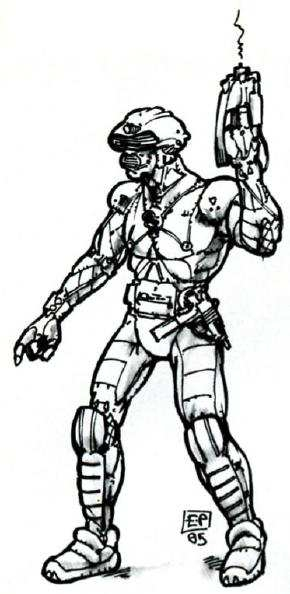
\includegraphics[width=0.30\textwidth]{img/persoRunnerGun.jpg}

\textbf{\textit{Pour CyberAge}}~\\

\texttt{Trois mini sc{\'e}narios}~\\

\textbf{Vengeance maya}~\\

Les personnages prennent le frais dans leur bar habituel, le Gentleman's Looser, quand un homme entre et d{\'e}sint{\`e}gre Pat Desnos, le patron et ami des PJ. Le tueur semble en transe et invuln{\'e}rable aux tirs de riposte des consommateurs, bien qu'il ne porte apparemment pas de gilet pareballes. Il est en effet enti{\`e}rement recouvert d'une armure nano qui le met {\`a} l'abri des tirs d'armes l{\'e}g{\`e}res. Il est {\'e}quip{\'e} d'un laser haute puissance avec deux charges seulement (il en a utilis{\'e} une) et d'un mini pistolet-mitrailleur au c{\^o}t{\'e}.~\\

Torr{\`e}s, l'homme en question, n'en est pas {\`a} son cou d'essai et ne frappe pas au hasard. Pat Desnos, sa septi{\`e}me victime, et tous les autres, {\'e}taient d'anciens Mercs qui avaient servi dans la m{\^e}me unit{\'e} lors des Guerres am{\'e}ricaines contre les rebelles mayas. Durant une op{\'e}ration, Torr{\`e}s fut s{\'e}rieusement bless{\'e}. Il a toujours pens{\'e} que ses camarades l'avaient abandonn{\'e} et depuis, il m{\^u}rit des projets de vengeance.~\\
Les personnages enqu{\^e}tent sur la mort de leur ami et l'identit{\'e} de son assassin.~\\

Profitez-en pour les lancer sur autant de fausses pistes que vous le d{\'e}sirez (racket des yakuzas, vieux ennemis, etc.) afin de cultiver la parano{\"i}a des joueurs. La v{\'e}rit{\'e} appara{\^i}t quand la fille de Desnos leur montre un vieil holo repr{\'e}sentant le squad de son p{\`e}re. On y reconna{\^i}t non seulement Torr{\`e}s, mais {\'e}galement toutes ses derni{\`e}res victimes. Trois hommes sont encore en vie, dont un riche repr{\'e}sentant d'un \texttt{TechnoBloc} de la c{\^o}te m{\'e}diterran{\'e}enne, le seul Merc ayant r{\'e}ussi socialement. Les personnages vont aller le trouver pour le mettre en garde. Ulysse Papandr{\'e}ous est un dur {\`a} cuire, et m{\^e}me s'il accepte d'engager les personnages, il ne fera rien pour {\'e}viter la confrontation avec Torr{\`e}s.~\\

Un des personnages finit par {\^e}tre captur{\'e} par Torr{\`e}s, qui le drogue et lui ordonne de ramener les autres dans son repaire pour s'en d{\'e}barrasser. Les PJ peuvent tomber ou non dans le pi{\`e}ge. Dans tous le cas, ils doivent retrouver Torr{\`e}s avant qu'il ne mette sa vengeance {\`a} ex{\'e}cution.~\\

\barreCyberAgeThird
\vfill
%% \columnbreak

\textbf{Zone de feu}~\\

Un des personnages aide Slide, un de ses amis d'enfance. Slide est un Sauvage urbain dont le clan est parvenu {\`a} f{\'e}d{\'e}rer plusieurs bandes d'une zone et arr{\^e}ter du coup la guerre qu'elles se livrent. Le personnage est attir{\'e} dans un hangar, drogu{\'e} par un Wampire, puis remis {\`a} un << Obeyin >>, un chef de clan yakuza qui ne voit pas d'un tr{\`e}s bon oeil l'entente cordiale qui se dessine dans sa zone d'influence (les ventes d'armes vont b{\^e}tement baisser).~\\

Asuma Korino, le yakuza, drogue le personnage pour le dresser {\`a} tuer Slide, le conditionnement est plus ou moins long selon la r{\'e}sistance du personnage. Pendant ce temps, on peut esp{\'e}rer que ses camarades finissent par retrouver le lieu de son enl{\`e}vement : des SDF l'ont vu entrer dans le hangar et jamais ressortir.~\\

Le reste du sc{\'e}nario est une course de vitesse entre le personnage conditionn{\'e} et les autres, puis le retour dans le labo des yakuzas pour y faire le m{\'e}nage.~\\

Bien entendu, la mort de Slide rallumerait la guerre des clans, et les personnages se retrouveraient pris entre deux feux, d{\'e}sign{\'e}s par tous comme les assassins de la paix.~\\

\barreCyberAgeThird
\vfill
\columnbreak

\textbf{La nuit des hologrammes}~\\

MediASsist se voit confier une mission : assurer la protection d'un juge ind{\'e}pendant de la ville de Paris.~\\

Plusieurs de ses coll{\`e}gues sont d{\'e}j{\`a} morts dans des conditions myst{\'e}rieuses, tous avaient re\c{c}u auparavant un petit cercueil en bois noir. Le juge assiste {\`a} un holo spectacle, quand un des hologrammes l'attaque et tente de le tuer. Les personnages interviennent et d{\'e}branchent rapidement le mat{\'e}riel. Ils ne savent quoi penser : c'est la premi{\`e}re fois qu'il est question d'une tentative d'assassinat via hologramme, qui par d{\'e}finition n'est qu'une source lumineuse inoffensive.~\\

En observant avec attention les bandes holo, les personnages parviennent {\`a} isoler une marque de fabrique, un petit {\'e}tablissement sur les quais de la Seine. Lorsqu'ils s'y rendent, ils sont pris dans une bagarre et disparaissent dans un sous-sol pi{\'e}g{\'e}. Un {\'e}lectronicien de g{\'e}nie les attend et les informe qu'il a mis au point une m{\'e}thode pour changer les hologrammes en lumi{\`e}re coh{\'e}rente (donc en laser), pendant une fraction de seconde seulement, mais c'est suffisant pour en faire des assassins parfaits. Il compte ainsi {\'e}liminer les juges de la ville qui l'ont condamn{\'e} il y a plusieurs ann{\'e}es a dix ans de bagne lunaire. Les personnages devront combattre les hologrammes laser pour d{\'e}couvrir {\`a} la fin que leur ma{\^i}tre est {\'e}galement un hologramme, l'{\'e}manation d'un programme d'intelligence artificielle ; le v{\'e}ritable informaticien est mort sur la Lune depuis longtemps...~\\

\barreCyberAgeThird

} % end footnotesize
\end{multicols*} 

\clearpage

\part*{R{\^e}gles Sp{\'e}ciales\markboth{R{\^e}gles Sp{\'e}ciales}{R{\^e}gles Sp{\'e}ciales}}
\addcontentsline{toc}{part}{R{\^e}gles Sp{\'e}ciales}

\begin{multicols*}{2}

\section*{R{\^e}gles Sp{\'e}ciales -- Cyber Age\markboth{R{\^e}gles Sp{\'e}ciales -- Cyber Age}{R{\^e}gles Sp{\'e}ciales -- Cyber Age}}
\addcontentsline{toc}{section}{R{\^e}gles Sp{\'e}ciales -- Cyber Age}

\textbf{\footnotesize Vous trouverez ci-apr{\`e}s les r{\`e}gles applicables {\`a} l'univers de \emph{Cyber Age}. Sauf lorsque cela est sp{\'e}cifi{\'e}, les r{\`e}gles g{\'e}n{\'e}rales de \emph{Simulacres} sont toujours appliqu{\'e}es. Vous trouverez donc : la cr{\'e}ation du pass{\'e} des personnages ; l'{\'E}quipement cybern{\'e}tique et les armements ; la gestion de l'univers informatique de la Matrice. } %% ~\\

%% \textbf{\Large Cr{\'e}ation de personnage}~\\
\subsection*{Cr{\'e}ation de personnage\markboth{Cr{\'e}ation de personnage}{Cr{\'e}ation de personnage}}
\addcontentsline{toc}{subsection}{Cr{\'e}ation de personnage}

Un personnage de \emph{Cyber Age} se d{\'e}finit avant tout par son pass{\'e} et ses capacit{\'e}s. On va donc les d{\'e}terminer  avant d'attribuer les valeurs des caract{\'e}ristiques {\`a} l'aide des r{\`e}gles g{\'e}n{\'e}rales de Simulacres. Au cas o{\`u} vous joueriez pour la premi{\`e}re fois dans un univers cyberpunk, nous vous conseillons plutot d'utiliser les personnages pr{\'e}tir{\'e}s fournis dans \emph{Cyber Age}. %% ~\\

%% \textbf{\large D{\'e}terminer son {\^a}ge}~\\
\subsubsection*{D{\'e}terminer son {\^a}ge\markboth{D{\'e}terminer son {\^a}ge}{D{\'e}terminer son {\^a}ge}}
\addcontentsline{toc}{subsubsection}{D{\'e}terminer son {\^a}ge}

Tout d'abord vous allez d{\'e}terminer l'{\^a}ge de votre personnage. Il peut avoir de 14 {\`a} 16 ans, de 17 {\`a} 30 ans, de 30 {\`a} 50 ans, ou plus de 50 ans. {\`A} vous de choisir (ou de tirer au hasard). 
\begin{itemize}
	\item[1] De 12 {\`a} 16 ans. Apr{\`e}s avoir d{\'e}termin{\'e} votre pass{\'e} (voir paragraphe suivant), d{\'e}terminez un m{\'e}tier et utiliser 12 points d'aventure (PA). Votre argent de d{\'e}part est tir{\'e} au sort. Lancez un d{\'e} (D6) et multipliez par 2000 euros (\euro ). 
	\item[2-3] De 17 {\`a} 30 ans. Apr{\`e}s avoir d{\'e}termin{\'e} votre pass{\'e} (voir paragraphe suivant), d{\'e}terminez un m{\'e}tier et utiliser 15 points d'aventure (PA). Votre argent de d{\'e}part est tir{\'e} au sort. Lancez un d{\'e} (D6) et multipliez par 1000~\euro ~et rajoutez 10 000~\euro. 
	\item[4-5] De 30 {\`a} 50 ans. Apr{\`e}s avoir d{\'e}termin{\'e} votre pass{\'e} (voir paragraphe suivant), d{\'e}terminez un m{\'e}tier et utiliser 18 points d'aventure (PA). Votre argent de d{\'e}part est tir{\'e} au sort. Lancez un d{\'e} (D6) et multipliez par 2000~\euro ~et rajoutez 30 000~\euro. 
	\item[6] Plus de 50 ans. Apr{\`e}s avoir d{\'e}termin{\'e} votre pass{\'e} (voir paragraphe suivant), d{\'e}terminez un m{\'e}tier et utiliser 21 points d'aventure (PA). Votre argent de d{\'e}part est tir{\'e} au sort. Lancez un d{\'e} (D6) et multipliez par 2000~\euro et rajoutez 5 000~\euro. Vous avez un point de moins en Corps, un point de plus en Instinct.  
\end{itemize} %% ~\\

%% \textbf{\large D{\'e}terminer son pass{\'e}}~\\
\subsubsection*{D{\'e}terminer son pass{\'e}\markboth{D{\'e}terminer son pass{\'e}}{D{\'e}terminer son pass{\'e}}}
\addcontentsline{toc}{subsubsection}{D{\'e}terminer son pass{\'e}}
Pour cela, vous allez devoir utiliser les tables des pages suivantes... ~\\~\\ %% de la double page suivante. ~\\~\\

\begin{itemize}
	\item[$\bullet$] Si vous avez de 17 {\`a} 50 ans, vous allez r{\'e}aliser six fois de suite la m{\^e}me proc{\'e}dure : lancer une fois deux d{\'e}s (D6) et consulter la Table d'Orientation (TO). Celle-ci vous donne une sous-table dans laquelle vous tirerez une situation au hasard en lan\c{c}ant ancore une fois deux d{\'e}s (D6). Vous obtenez ainsi six situations, avec leurs avantages et inconv{\'e}nients, que vous pouvez arranger dans l'ordre chronologique que vous d{\'e}sirez. Si vous tirez deux fois une m{\^e}me situation, vous ne l'utilisez qu'une fois. Si vous la tirez trois fois, tirez {\`a} nouveau; Vous devez utiliser toutes les situations. 
	\item[$\bullet$] Si vous avez de 12 {\`a} 16 ans, ne tirez que trois situations. --- Si vous avez plus de 50 ans, tirez huit situations, mais n'en choisissez que six. 
\end{itemize} ~\\

\textbf{\large Que vous apportent ces tables : } %% ~\\
%% \subsubsection*{ALLAsubsubsect\markboth{ALLAsubsubsect}{ALLAsubsubsect}}
%% \addcontentsline{toc}{subsubsection}{ALLAsubsubsect}
\begin{itemize}
	\small
	\item Certaines situations impliquent un bonus ou un malus aux capacit{\'e}s du personnage. Il est indiqu{\'e} {\`a} chaque fois. 
	\item Certaines situations donnent la possibilit{\'e} de faire un certain m{\'e}tier (s'il y a un \emph{\textbf{M+}} entre parenth{\`e}ses) ou en interdisent d'autres (un \emph{\textbf{M-}} entre parenth{\`e}ses). Si vous n'avez aucun \emph{\textbf{M+}}, vous choisissez le m{\'e}tier que vous d{\'e}sirez sans p{\'e}nalit{\'e}s. Si vous voulez choisir un m{\'e}tier autre que celui qui vous est sugg{\'e}r{\'e}, cela vous co{\^u}tera 5 PA. 
	\item Si vous choisissez un m{\'e}tier, vous poss{\'e}dez automatiquement tous les talents propres {\`a} ce m{\'e}tier au niveau 0 \emph{(50\%)} (sauf pour CyberTek, voir la description de ce m{\'e}tier), et vous ne b{\'e}n{\'e}ficiez donc pas des talents suppl{\'e}mentaires propos{\'e}s pour celui-ci. Par contre, l'un de ces talents sera au niveau +1 \emph{(60-75\%)} ({\`a} votre choix). 
	\item Lors qu'on vous propose un talent suppl{\'e}mentaire (et qui n'est pas votre m{\'e}tier), vous pouvez toujours le prendre comme un talent qui vous appartient en propre (en le mettant au niveau 0 et en d{\'e}pensant 1 PA), ou en logiciel caillou si vous avez une broche (sans d{\'e}penser de PA). 
	\item Un \emph{\textbf{{\'E}q.}} dans les cons{\'e}quences indique que le personnage b{\'e}n{\'e}ficie s'il le d{\'e}sire d'un {\'e}quipement cybern{\'e}tique. Il le tire au hasard dans la Table d'{\'E}quipements (TE). S'il refuse (avant de tirer au hasard), il peut choisir {\`a} la place 3 Points d'Aventure. 
	\item Un \emph{\textbf{Pa}} dans les cons{\'e}quences indique que vous pouvez avoir un <<parrain>> dans cette profession. Vous ne pouvez avoir plus d'un parrain ou m{\^e}me d{\'e}cider d'en avoir aucun. Un parrain est une personne que vous connaissez bien dans un certain milieu, et qui est susceptible de vous donner des informations. C'est utile pour vous tirer de mauvais pas, mais ce parrain peut vous demander des services en {\'e}change.  
\end{itemize} %% ~\\

\clearpage
%% DONE ins{\'e}rer tables passe... ++ table d'equipement... !!

\textbf{Table d'Orientation \dotfill } ~\\
\begin{minipage}[ht]{0.25\textwidth}
	\begin{enumerate}
		\footnotesize
		\item[2] Table Espace-Venise
		\item[3] Table Network
		\item[4] Table Jackeur
		\item[5] Table BladeRunner
		\item[6] Table Divers
		\item[7] Table Gangs
		\item[8] Table Divers
		\item[9] Table Yakuza
		\item[10] Table R{\^o}nin
		\item[11] Table TechnoBloc
		\item[12] Table Wampire-R{\^e}veur
	\end{enumerate} 
\end{minipage} \hfill \begin{minipage}[ht]{0.25\textwidth}
	\colorbox{verylightgrey}{ \framebox{ \footnotesize %
	\begin{minipage}[ht]{0.75\textwidth}
		\textbf{L{\'e}gende}~\\
		\textbf{M+ : }Possibilit{\'e} de choisir ce m{\'e}tier. ~\\
		\textbf{M- : }Interdiction de choisir ce m{\'e}tier. ~\\
		\textbf{{\'E}q. : }Un {\'e}quipement cybern{\'e}tique {\`a} tirer au hasard. ~\\
		\textbf{Pa : }Possibilit{\'e} de choisir un parrain dans le domaine. ~\\
	\end{minipage} } } % 
\end{minipage}

~\\ \barreCyberAgeHalf %% ~\\

\textbf{Table Espace-Venise \dotfill 2 } ~\\
	\emph{\footnotesize Donne acc{\`e}s au m{\'e}tier de Cybertek, dans des domaines vari{\'e}s. } %% ~\\
\begin{enumerate}
	\footnotesize
	\item[2] Vous faites naufrage en plein espace. Vous restez un an et demi en Synthivers. Vous perdez 1 point en {\'E}quilibre Psychique. Choisissez un talent de CyberTek. (\textbf{M+})
	\item[3] Vous passez plusieurs mois dans une Venise. Choisissez un talent de CyberTek. (\textbf{M+})
	\item[4] Vous signez un contrat de mineur pour deux ans en Espace profond. Choisissez deux talent de CyberTek. (\textbf{M+}, \textbf{{\'E}q.})
	\item[5] Vous {\^e}tes engag{\'e}(e) pour un travail temporaire dans une Venise. Choisissez un talent de CyberTek. (\textbf{M+}, \textbf{{\'E}q.})
	\item[6] Vous passez plusieurs mois sur une base spatiale. Choisissez un talent de CyberTek. (\textbf{M+}, \textbf{{\'E}q.})
	\item[7] Vous suivez une formation {\`a} la Fondation comme m{\'e}canicien spatial. Choisissez deux talent de CyberTek. (\textbf{M+}, \textbf{Pa})
	\item[8] Dans une Venise, vous avez une liaison avec une Sir{\`e}ne (ou un Triton). Tirez sur la table de Romance. (\textbf{Pa})
	\item[9] {\`A} la suite d'une bonne affaire, vous achetez une petite usine {\`a} soma, en bord de mer. Revenu mensuel net de 6 000 cr{\'e}dits ! Choisissez un talent de CyberTek. 
	\item[10] Vous devenez plongeur pendant quelques mois. Choisissez un talent de CyberTek. (\textbf{M+}, \textbf{{\'E}q.})
	\item[11] Un(e) Phase II a failli vous tuer. Si vous le (la) croiser, vous essayerez de vous venger. 
	\item[12] Vous faites naufrage en pleine mer. Vous n'{\^e}tes r{\'e}cup{\'e}r{\'e}(e) qu'un mois apr{\`e}s, sur une {\^i}le presque d{\'e}serte. Vous gagnez un point suppl{\'e}mentaire en R{\`e}gne Animal, V{\'e}g{\'e}tal ou Min{\'e}ral. 
\end{enumerate}

\textbf{Table Network \dotfill 3 } ~\\
	\emph{\footnotesize Donne acc{\`e}s au m{\'e}tier d'holoreporter ou de pilote de voile solaire. } %% ~\\
\begin{enumerate}
	\footnotesize
	\item[2] Vous participez {\`a} une action terroriste. Choisissez un talent de Mercenaire. (\textbf{Pa})
	\item[3] Vous avez une liaison avec un(e) HoloReporter. Tirez sur la table de Romance. (\textbf{Pa})
	\item[4] Vous devenez Pilote de voile Solaire. Choisissez un talent de Pilote. (\textbf{M+}, \textbf{{\'E}q.})
	\item[5] Vous participez {\`a} une Chasse. Choisissez un talent {\`a} votre convenance. (\textbf{{\'E}q.})
	\item[6] Vous {\^e}tes la cible d'une Chasse. Vous tuez votre Chasseur. Choisissez deux talents {\`a} votre convenance
	\item[7] Vous r{\'e}alisez une vid{\'e}o sur un attentat terroriste qui est diffus{\'e} sur un Network. Choisissez un talent d'Holoreporter. (\textbf{M+}, \textbf{{\'E}q.})
	\item[8] Vous avez une liaison avec un(e) terroriste. Tirez sur la table de Romance. (\textbf{Pa})
	\item[9] Vous avez une liaison avec un(e) Pilote (Voile Solaire ou HoverTank). Tirez sur la table de Romance. (\textbf{Pa})
	\item[10] Vous contractez une dette vis-{\`a}-vis d'un groupe terroriste. Il peut vous demander son remboursement {\`a} tout moment. 
	\item[11] Un groupe terroriste a une dette vis-{\`a}-vis de vous. Vous pouvez lui demander un service. 
	\item[12] Vous {\^e}tes victime d'un attentat terroriste. Tirez sur la table des Cicatrices. 
\end{enumerate}

\textbf{Table Jackeur \dotfill 4 } ~\\
	\emph{\footnotesize Donne acc{\`e}s au m{\'e}tier de jackeur. } %% ~\\
\begin{enumerate}
	\footnotesize
	\item[2] Une Dactyle vous {\'e}duque. Choisissez deux talents de Jackeur. (\textbf{Pa}, \textbf{M+})
	\item[3] Vous {\'e}chappez de justesse {\`a} un logiciel tueur. Vous perdez 1 point en {\'E}quilibre Psychique). (\textbf{M+})
	\item[4] Un Jackeur a essay{\'e} de vous entuber. Vous essayerez de vous venger de lui. 
	\item[5] Un de vos amis Jackeur vous a laiss{\'e} un programme BriseGlace (au choix) avant de partir dans l'espace. 
	\item[6] Vous travaillez pour un Jackeur fortun{\'e} qui vous paye en nature. Vous r{\'e}cup{\'e}rez un programme au choix (sauf BriseGlace). (\textbf{{\'E}q.} ; \textbf{M+})
	\item[7] Vous devenez l'ami d'un Jackeur qui meurt apr{\`e}s un combat en Matrice / Cyberespace. Vous r{\'e}cup{\'e}rez sa Console. Mod{\`e}le XX. 
	\item[8] Vous vous faites un ennemi d'un Jackeur. Il peut chercher {\`a} vous attaquer s'il vous rencontre dans la Matrice / le REZO. 
	\item[9] Vous avez une liaison avec un(e) Jackeur. Tirez sur la table de Romance. 
	\item[10] Vous contractez une dette vis-{\`a}-vis d'un Jackeur. Il peut vous demander son remboursement {\`a} tout moment. 
	\item[11] Un Jackeur a une dette vis-{\`a}-vis de vous. Vous pouvez lui demander un service. 
	\item[12] Sans le vouloir, vous aidez une Intelligence Artificielle. Elle vous contacte et dit qu'elle pourra vous aider une fois, lorsque vous le d{\'e}sirerez, dans la Matrice / le REZO. 
\end{enumerate}

\textbf{Table BladeRunner \dotfill 5 } ~\\
	\emph{\footnotesize Donne acc{\`e}s au m{\'e}tier de bladerunner. } %% ~\\
\begin{enumerate}
	\footnotesize
	\item[2] Vous faites {\'e}quipe plusieurs mois avec un(e) BladeRunner. Tirez sur la table de Romance. Choisissez deux talents de BladeRunner. (\textbf{Pa}, \textbf{M+})
	\item[3] Un(e) BladeRunner vous enseigne ce qu'il (elle) sait. Choisissez deux talents de BladeRunner. (\textbf{Pa}, \textbf{M+})
	\item[4] Vous {\^e}tes arr{\^e}t{\'e} par un(e) BladeRunner. Tirez sur la table Prison. 
	\item[5] Lors d'une op{\'e}ration mercenaire, vous {\^e}tes trahi(e) par un(e) BladeRunner. Vous vous en sortez. Tirez sur la table des Cicatrices. 
	\item[6] Vous avez une liaison avec un(e) BladeRunner. Tirez sur la table de Romance. (\textbf{Pa})
	\item[7] Une agence de Mercs vous apprend les rudiments du m{\'e}tier de BladeRunner. Choisissez un talent de BladeRunner. (\textbf{{\'E}q.}, \textbf{M+})
	\item[8] Vous tuez un(e) BladeRunner. Tirez sur la table des Cicatrices. 
	\item[9] Vous {\^e}tes poursuivi(e) par un BladeRunner. Il peut vous rattraper {\`a} tout moment. 
	\item[10] Vous contractez une dette vis-{\`a}-vis d'un BladeRunner. Il peut vous demander son remboursement {\`a} tout moment. 
	\item[11] Un BladeRunner a une dette vis-{\`a}-vis de vous. Vous pouvez lui demander un service. (\textbf{Pa})
	\item[12] Une agence de d{\'e}tectives vous apprend les rudiments du m{\'e}tier de BladeRunner. Choisissez un talent de BladeRunner. (\textbf{{\'E}q.}, \textbf{M+})
\end{enumerate}

\textbf{Table Divers \dotfill 6 / 8 } %% ~\\
\begin{enumerate}
	\footnotesize
	\item[2] Vous perdez votre famille lorsque vous {\^e}tes tr{\`e}s jeune. 
	\item[3] Vous participez {\`a} une course d'hovertanks. Vous gagnez un talent de conduite. 
	\item[4] Vous gagnez lors d'un concours l'arme personnelle de votre choix. 
	\item[5] Vous gagnez un s{\'e}jour d'un mois sur les {\^I}les de la Lune. Choisissez un talent de CyberTek. 
	\item[6] Vous vous droguez durement. Vous perdez un point en {\'E}quilibre Psychique. 
	\item[7] Vous gagnez 50 000 cr{\'e}dits en pariant sur une course de voiles solaires. 
	\item[8] Vous devenez c{\'e}l{\`e}bre pendant 2 semaines. {\`A} vous d'en inventer la raison. 
	\item[9] Vous avez un tr{\`e}s grave accident. Tirez sur la table des Cicatrices. 
	\item[10] Vous gagnez lors d'un concours, n'importe quel type de cablage (sauf cablage total). 
	\item[11] Vous passez votre jeunesse dans une tr{\`e}s bonne {\'e}cole. Choisissez deux talentssuppl{\'e}mentaires dans la table g{\'e}n{\'e}rale ou dans le m{\'e}tier de CyberTek. 
	\item[12] Vous {\^e}tes testeur d'onirogrammes pendant un an. Vous avez une broche de type C et six cailloux d'onirogramme.  
\end{enumerate}

\textbf{Table Gangs \dotfill 7 } %% ~\\
\begin{enumerate}
	\footnotesize
	\item[2] Vous passez une partie de votre adolescence dans un Gang. Choisissez un tament appropri{\'e}. (\textbf{Pa})
	\item[3] Vous devenez l'ennemi d'un chef de Gang. Faites attention quand vous passez sur son territoire. 
	\item[4] Vous devenez l'ami d'un chef de Gang. (\textbf{Pa})
	\item[5] Des Yakuzas remarquent vos capacit{\'e}s. Tirez sur la table des Yakuzas. 
	\item[6] Vous contractez une dette vis-{\`a}-vis d'un chef de Gang. Il peut vous demander son remboursement {\`a} tout moment. 
	\item[7] Un chef de Gang a une dette vis-{\`a}-vis de vous. Vous pouvez lui demander un service. (\textbf{Pa})
	\item[8] Vous tombez amoureux(se) d'un membre de Gang. Tirez sur la table de Romance. (\textbf{Pa})
	\item[9] Vous {\^e}tes bless{\'e}(e) dans un combat de rue. Tirez sur la table des Cicatrices. 
	\item[10] Vous devenez chef de Gang pendant quelques mois. Vous pouvez faire appel aux anciens membres du Gang. Choisissez deux talents qui vous semblent appropri{\'e}s. (\textbf{{\'E}q.})
	\item[11] Vous {\^e}tes arr{\^e}t{\'e}(e) par une milice de TechnoBloc pour activit{\'e}s ill{\'e}gales au sein d'un Gang. Tirez sur la table Prison. 
	\item[12] Vous passez une partie de votre adolescence dans un Gang. Choisissez un tament appropri{\'e}. (\textbf{Pa})
\end{enumerate}

\textbf{Table Yakuza \dotfill 9 } ~\\
	\emph{\footnotesize Donne acc{\`e}s {\`a} l'appartenance au yakuza. } %% ~\\
\begin{enumerate}
	\footnotesize
	\item[2] Un Yakuza a failli vous tuer. Vous essayez de vous venger et tenterez de le tuer s'il croise votre chemin. 
	\item[3] Un Yakuza vous enseigne ce qu'il (elle) sait. Choisissez un talent de Yakuza. (\textbf{Pa}, \textbf{M+})
	\item[4] Vous {\^e}tes arr{\^e}t{\'e}(e) {\`a} la place d'un Yakuza. Tirez sur la table Prison. (\textbf{M+})
	\item[5] Vous {\^e}tes trahi(e) par un Yakuza qui manque de vous tuer. Tirez sur la table des Cicatrices. 	(\textbf{M-})
	\item[6] Vous {\^e}tes victime d'une arnaque Yakuza sur des paris. Vous commencez l'aventure sans le sou. 
	\item[7] Vous devenez Yakuza pendant quelques mois. Choisissez un talent de Yakuza. (\textbf{M+}, \textbf{{\'E}q.}, \textbf{Pa})
	\item[8] Vous tuez un yakuza. 	[Cicatrices] (\textbf{M-})
	\item[9] Un contrat a {\'e}t{\'e} lanc{\'e} sur vous par les Yakuzas. Ils peuvent vous rattraper {\`a} tout moment. (\textbf{M-})
	\item[10] Vous contractez une dette vis-{\`a}-vis d'un Yakuza. Il peut vous demander son remboursement {\`a} tout moment. 
	\item[11] Un Yakuza a une dette vis-{\`a}-vis de vous. Vous pouvez lui demander un service. (\textbf{Pa})
	\item[12] Vous travaillez un temps pour le Yakuza, puis vous le d{\'e}sertez. Il vous est d{\'e}sormais impossible de travailler pour le Yakuza. Choisissez un talent de Yakuza. (\textbf{M-})
\end{enumerate}

\textbf{Table R{\^o}nin \dotfill 10 } ~\\
	\emph{\footnotesize Donne acc{\`e}s au m{\'e}tier de r{\^o}nin ou de mercenaire. } %% ~\\
\begin{enumerate}
	\footnotesize
	\item[2] Vous cherchez {\`a} vous venger d'un R{\^o}nin. 
	\item[3] Un R{\^o}nin vous enseigne ce qu'il (elle) sait. Choisissez un talent de R{\^o}nin. (\textbf{Pa}, \textbf{M+})
	\item[4] Vous {\^e}tes bless{\'e}(e) lors d'une Guerre Priv{\'e}e. Tirez sur la table des Cicatrices. 
	\item[5] Vous {\^e}tes trahi(e) par une Mercenaire. Vous cherchez {\`a} vous venger. Tirez sur la table des Cicatrices. 
	\item[6] Vous avez une liaison avec un(e) R{\^o}nin. Tirez sur la table de Romance. (\textbf{Pa})
	\item[7] Vous devenez Mercenaire pendant quelques mois. Choisissez deux talents de Mercenaire. (\textbf{M+}, \textbf{{\'E}q.})
	\item[8] Vous tuez un R{\^o}nin. Tirez sur la table des Cicatrices. 
	\item[9] Vous {\^e}tes poursuivi(e) par un R{\^o}nin. Il peut vous rattraper {\`a} tout moment. 
	\item[10] Vous contractez une dette vis-{\`a}-vis d'un R{\^o}nin. Il peut vous demander son remboursement {\`a} tout moment. 
	\item[11] Un R{\^o}nin a une dette vis-{\`a}-vis de vous. Vous pouvez lui demander un service. (\textbf{Pa})
	\item[12] Vous devenez Mercenaire pendant quelques mois dans une Force tr{\`e}s c{\^o}t{\'e}e. Choisissez deux talents de Mercenaire. (\textbf{M+}, \textbf{{\'E}q.}, \textbf{Pa})
\end{enumerate}

\textbf{Table TechnoBloc \dotfill 11 } ~\\
	\emph{\footnotesize Donne acc{\`e}s au m{\'e}tier de cybertek. } %% ~\\
\begin{enumerate}
	\footnotesize
	\item[2] Vous {\^e}tes vir{\'e} de votre TechnoBloc. Tirez {\`a} nouveau sur cette table pour votre nouveau TechnoBloc. 
	\item[3] Vous {\^e}tes exfiltr{\'e}(e) de votre TechnoBloc. Choisissez deux talents de CyberTek. Tirez sur la table des Cicatrices. (\textbf{M+}, \textbf{{\'E}q.})
	\item[4] Vous vous faites des relations dans votre TechnoBloc. 	{Parrain:CyberTek||TechnoBloc}
	\item[5] Vous vous faites des ennemis dans votre TechnoBloc. 
	\item[6-7] Vous acc{\'e}dez {\`a} un poste de cadre dans votre TechnoBloc. Choisissez deux talents de CyberTek. (\textbf{M+}, \textbf{{\'E}q.}, \textbf{Pa})
	\item[8-9] Votre TechnoBloc vous offre un cablage gratuit. (\textbf{{\'E}q.})
	\item[10] Vous aidez un ami {\`a} s'exfiltrer de son TechnoBloc. Il vous en est redevable.
	\item[11] Vous avez une liaison avec un(e) cadre d'un TechnoBloc. Tirez sur la table de Romance. (\textbf{Pa})
	\item[12] Vous {\^e}tes vir{\'e}(e) de votre TechnoBloc. Tirez {\`a} nouveau sur cette table pour votre nouveau TechnoBloc. 
\end{enumerate}

\vfill
\columnbreak

\textbf{Table Wampire-R{\^e}veur \dotfill 12 } ~\\
	\emph{\footnotesize Donne acc{\`e}s aux m{\'e}tiers de r{\'e}veur ou de wampire. } %% ~\\
\begin{enumerate}
	\footnotesize
	\item[2] Vous vendez vos r{\^e}ves pendant quelques mois. Moins 1 en {\'E}quilibre Psychique, Talent Onirisme {\`a} +1. (\textbf{M+}, \textbf{{\'E}q.})
	\item[3] Un ami r{\^e}veur devient fou. Vous ne supportez plus les usines {\`a} r{\^e}ves. 
	\item[4] Vous tuez un wampire. 
	\item[5] Un de vos amis est tu{\'e} par un Wampire. Vous les d{\'e}testez. 
	\item[6] Vous c{\'e}dez un de vos organes {\`a} un Wampire. Moins 1 en Corps. 
	\item[7] Vous exfiltrez un de vos amis d'une usine {\`a} r{\^e}ves. 
	\item[8] Vous exercez le m{\'e}tier de Wampire pendant quelques mois. Choisissez un talent de Wampire. (\textbf{M+}, \textbf{Pa})
	\item[9] Vous avez une liaison avec un(e) R{\^e}veur. Tirez sur la table de Romance. 
	\item[10] Vous contractez une dette vis-{\`a}-vis d'un Wampire. Il peut vous demander son remboursement {\`a} tout moment. 
	\item[11] Un Wampire a une dette vis-{\`a}-vis de vous. Vous pouvez lui demander un service. (\textbf{Pa})
	\item[12] Vous devenez pendant quelques mois une star des usines {\`a} r{\^e}ves. Vous vous {\'e}chappez. Vous poss{\'e}dez 30 000 000 de cr{\'e}dits. Votre {\'e}quilibre psychique est au minimum (remont{\'e}e possible avec traitement psychiatrique). Vous ne supportez pas l'id{\'e}e que l'on puisse vous rajouter un {\'e}quipement cybern{\'e}tique. Vous avez perdu 1 en Esprit. Votre {\'E}quilibre Psychique vaut 1. Vous avez les talents suivants : Onirisme +2, Connaissance des Medias +1. 
\end{enumerate}

~\\ \barreCyberAgeHalf ~\\

\vfill ~\\
\columnbreak

\textbf{Table Romance \dotfill } ~\\
	\textbf{\footnotesize Tirez avec un d{\'e}} %% ~\\
\begin{enumerate}
	\footnotesize
	\item[1] Votre liaison vous trahit. Vous la ha{\"i}ssez. 
	\item[2] Vous vous f{\^a}chez. Vous vous quittez en bons termes. 
	\item[3] Vous vous quittez. Mais vous restez en bons termes. 
	\item[4] Votre liaison dispara{\^i}t. Vous en {\^e}tes toujours amoureux(se). Peut-{\^e}tre reviendra-t-elle (il) ? 
	\item[5] Vous trahissez votre liaison. Elle (Il) vous hait. 
	\item[6] Votre liaison meurt. Tirez un d{\'e} et consultez la table suivante. 
\end{enumerate}

	\textbf{\footnotesize Votre liaison meurt...} %% ~\\
\begin{enumerate}
	\footnotesize
	\item[1] Dans un accident. Vous en avez un immense chagrin. 
	\item[2] Suite {\`a} un suicide. Vous en avez un immense chagrin. 
	\item[3] Suite {\`a} une overdose. Vous d{\'e}testez les dealers. 
	\item[4] Assassin{\'e}(e) par un gang. Vous pr{\'e}parez une vengeance. 
	\item[5] Assassin{\'e}(e) par des yakuzas. Vous pr{\'e}parez une vengeance. 
	\item[6] Assassin{\'e}(e) dans une guerre priv{\'e}e. Vous pr{\'e}parez peut-{\^e}tre une vengeance contre les Mercs responsables. 
\end{enumerate}

~\\ \barreCyberAgeHalf ~\\

\textbf{Table Prison \dotfill } %% ~\\
\begin{enumerate}
	\footnotesize
	\item[1] Vous {\^e}tes emprisonn{\'e}(e) pour un an dans un MurMorgue. Vous gagnez au choix l'un des talents suivants : {Couture+1 ; Tricot+1 ; Cuisine+1 ; Nettoyage+1 ; SavoireVivre+0}.
	\item[2] Vous {\^e}tes emprisonn{\'e}(e) dans un p{\'e}nitencier. Vous vous {\'e}vadez au bout de deux ans.  
	\item[3] Vous {\^e}tes emprisonn{\'e}(r) dans un p{\'e}nitencier. Vous tentez de vous {\'e}vader et vous {\'e}chouez. Vous sortez au bout de trois ans. 	[Cicatrices]
	\item[4] Vous passez trois ans sur un ast{\'e}ro{\"i}de minier. 	[Cicatrices]
	\item[5] Vous passez trois ans sur un ast{\'e}ro{\"i}de minier. Vous perdez 1 point en R{\'e}sistance. Vous gagnez les talents : {D{\'e}placement spatial+1 ; Survie dans l'espace+1}
	\item[6] Vous passez cinq ans en mine sous-marine. Vous perdez un point en C\oe ur. Vous gagnez les talents : {Plong{\'e}e+1 ; Survie sous-marine+1}
\end{enumerate}

~\\ \barreCyberAgeHalf ~\\

\textbf{Table Cicatrices \dotfill } ~\\
	\textbf{\footnotesize Localisation} %% ~\\
\begin{enumerate}
	\footnotesize
	\item[1] T{\^e}te. 
	\item[2] Torse. 
	\item[3] Bras gauche. 
	\item[4] Bras droit. 
	\item[5] Jambe gauche. 
	\item[6] Jambe droite. 
\end{enumerate}

	\textbf{\footnotesize Gravit{\'e}} %% ~\\
\begin{enumerate}
	\footnotesize
	\item[1] {\`A} peine visible. 
	\item[2-4] Cicatrice normale. 
	\item[5] Cicatrice tr{\`e}s visible et profonde. 
	\item[6] Perte d'une partie ou totalit{\'e} du membre. Pose d'une proth{\`e}se de remplacement. 
\end{enumerate}

\clearpage

Contrairement {\`a} d'autres univers, la sc{\'e}narisation du pass{\'e} des personnages n'est pas une option, elle fait partie int{\'e}grante de \emph{Cyber Age}. Il en d{\'e}coule le m{\'e}tier du personnage, son {\'e}quipement de d{\'e}part, ses amiti{\'e}s et inimiti{\'e}s. %% ~\\
 
%% \textbf{\large Exemple}~\\
\subsubsection*{Exemple\markboth{Exemple}{Exemple}}
\addcontentsline{toc}{subsubsection}{Exemple}
Philippe Bernard cr{\'e}e le personnage John Jennings. Il a 25 ans. 
\begin{itemize}
	\item[A)] 1/3 : Vous travaillez dans une base spatiale. 
	\item[B)] 10/5 : Trahi par un mercenaire, ce qui implique un membre artificiel et une vengeance. 
	\item[C)] 12/5 : Un ami tu{\'e} par un Wampire. 
	\item[D)] 4/5 : H{\'e}rite d'un programme BriseGlace. 
	\item[E)] 9/4 : Arr{\^e}t{\'e} {\`a} la place d'un yakuza, trois ans d'ast{\'e}ro{\"i}de minier, une cicatrice {\`a} peine visible et une dette du yakuza. 
	\item[F)] 12/3 : Un ami r{\^e}veur devient fou. 
\end{itemize}~\\

\textbf{Voici comment Philippe sc{\'e}narise les {\'e}v{\`e}nements : }~\\
John Jennings est employ{\'e} d{\`e}s l'{\^a}ge de 16 ans dans les {\^I}les de la Lune (A). Il se lie avec les yakuzas qui lui propose un casse dans la banque d'une des {\^I}les (E). Jennings accepte, il doit trouver une grosse somme d'argent pour la cure de d{\'e}sintoxication d'un ami r{\^e}veur (F). Le casse se passe mal, Jennings est bless{\'e} (B), son co{\'e}quipier, un mercenaire ind{\'e}pendant, l'abandonne derri{\`e}re lui (B). Arr{\^e}t{\'e}, Jennings ne parle pas, ce qui lui vaut la consid{\'e}ration du yakuza et la s{\'e}v{\'e}rit{\'e} du jury (E), il passe deux ans dans la mine ast{\'e}ro{\"i}de Jupiter V, il y contracte une maladie pulmonaire (E), on l'op{\`e}re des poumons et on lui greffe un bras artificiel (B). ~\\

Durant son s{\'e}jour en ast{\'e}ro{\"i}de, il se lie d'amiti{\'e} avec un vieux jackeur qui lui l{\`e}gue, avant de mourir, un programme BriseGlace (D). Lorsque Jennings est lib{\'e}r{\'e}, il d{\'e}cide de descendre sur Terre {\`a} la recherche du mercenaire f{\'e}lon. Les yakuzas lui procurent un poste de responsabilit{\'e} dans les jeux clandestins (E). Dans le milieu, on dit que Jennings porte la poisse, un de ses amis trouve la mort dans une ruelle sous le couteau d'un wampire qui lui vole son c\oe ur (C). ~\\

Le profil de Jennings : endurci par ses ann{\'e}es de mines (E) et la perte de ses amis (C, D, F), Jennings est un dur, pas bavard (E), appliquant {\`a} la lettre son code de l'honneur (E). Il a coutume de r{\'e}gler ses affaires tout seul (B). Il est anim{\'e} d'un puissant d{\'e}sir de vengeance (B). Il d{\'e}teste les flics (E), les Usines {\`a} R{\^e}ves (F) et les wampires (C). Il entretien de bons rapports avec les yakuzas sans en {\^e}tre un esclave (E). ~\\

\vfill ~\\ %% \columnbreak

Physiquement, les ann{\'e}es de mines l'ont us{\'e}e pr{\'e}matur{\'e}ment, il conserve son bras artificiel de mauvaise qualit{\'e} comme une sorte de d{\'e}fi, pour se souvenir de ses ann{\'e}es d'enfer. Petit, r{\^a}bl{\'e}, son regard froid et d{\'e}termin{\'e} arr{\^e}te bien souvent ceux qui veulent lui chercher des noises, il est pris de fr{\'e}quentes quintes de toux qu'il soigne discr{\`e}tement {\`a} coups de vodka. ~\\

Reste, toujours selon les tables, {\`a} choisir son {\'E}quipement cybern{\'e}tique, {\'e}ventuellement, son ou ses parrains et ses talents. %% ~\\

%% \textbf{\large Le mat{\'e}riel}~\\
\subsubsection*{Le mat{\'e}riel\markboth{Le mat{\'e}riel}{Le mat{\'e}riel}}
\addcontentsline{toc}{subsubsection}{Le mat{\'e}riel}
En ce qui concerne les {\'e}quipements tir{\'e}s au sort, il s'agit toujours du mod{\`e}le standard. Si le personnage veut b{\'e}n{\'e}ficier d'un mat{\'e}riel haut de gamme, il doit payer la diff{\'e}rence. Reportez-vous plus loin au catalogue qui explique les diverses possibilit{\'e}s des {\'e}quipements. Un \texttt{jackeur} a toujours comme premier {\'e}quipement un c{\^a}blage d'interface. {\`A} la place de tirer sur cette table ensuite, il peut choisir n'importe quel logiciel standard (sauf un BriseGlace, qui vaut deux logiciels). ~\\

\colorbox{verylightgrey}{ %
\begin{minipage}[h]{0.48\textwidth}
	\footnotesize
	\textbf{\large Table d'{\'E}quipement (TE)}%% ~\\
	\begin{itemize}
		\item[1] \OE il artificiel (voir sous-table). 
		\item[2] C{\^a}blage de combat (voir sous-table).  
		\item[3] C{\^a}blage auditif (voir sous-table). 
		\item[4] G.O.S.T. (mod{\`e}le de combat si vous tirez deux fois de m{\^e}me num{\'e}ro). 
		\item[5-6] Une broche de type A ou B, un caillou au choix. 
	\end{itemize}~\\
	
	\textbf{\OE il artificiel (un seul \oe il {\`a} la fois)} %% ~\\
	\begin{itemize}
		\item[1] Acquisiteur de cible. Avec interface radio sur une arme. Interface sous-cutan{\'e}e {\`a} acheter en sus.  
		\item[2] Vision infrarouge. 
		\item[3] Amplificateur d'image. 
		\item[4] T{\'e}l{\'e}objectif. 
		\item[5] Enregistreur vid{\'e}o. 
		\item[6] Radar. 
	\end{itemize}~\\
	
	\textbf{C{\^a}blage de combat} %% ~\\
	\begin{itemize}
		\item[1] Broche de type A ou B. Quatre cailloux de maniement d'armes. 
		\item[2] C{\^a}blage musculaire. 
		\item[3] C{\^a}blage nerveux (vitesse). 
		\item[4] M{\'e}taGriffes. 
		\item[5] {\'E}jecteur de gaz. 
		\item[6] Proth{\`e}se ou membre blind{\'e}. 
	\end{itemize}~\\
	
	\textbf{C{\^a}blage auditif} %% ~\\
	\begin{itemize}
		\item[1] R{\'e}seau t{\'e}l{\'e}phonique. 
		\item[2] Scanner radio. 
		\item[3] D{\'e}tecteur {\'e}lectronique. 
		\item[4] Enregistreur audio. 
		\item[5] Talkie-Walkie. 
		\item[6] Tirez deux {\'e}quipements sur cette m{\^e}me table. 
	\end{itemize} %% ~\\
\end{minipage} }% 

\vfill
\columnbreak

%% \textbf{\large Les caract{\'e}ristiques}~\\
\subsubsection*{Les caract{\'e}ristiques\markboth{Les caract{\'e}ristiques}{Les caract{\'e}ristiques}}
\addcontentsline{toc}{subsubsection}{Les caract{\'e}ristiques}
En suivant les r{\`e}gles g{\'e}n{\'e}rales de \emph{Simulacre}, choisissez maintenant les caract{\'e}ristiques de votre personnage. N'oubliez pas de retirer des points si la pass{\'e} du personnage en fait mention, et ceci apr{\`e}s les avoir r{\'e}partis. --- Ensuite, reportez-vous au chapitre sur les {\'E}quipements cybern{\'e}tiques pour conna{\^i}tre les cons{\'e}quences de l'implantation de ce mat{\'e}riel sur le personnage. Ces cons{\'e}quences sont valables dans le cours de l'aventure mais aussi d{\`e}s la cr{\'e}ation. --- Enfin, vous pouvez d{\'e}penser des Points d'Aventure pour acheter des talents {\`a} votre personnage. %% ~\\
%% Les bar{\`e}mes sont donn{\'e}s page 53 (r{\`e}gles g{\'e}n{\'e}rales de Simulacres). %% ~\\

%% \textbf{\large Talents particuliers}~\\
\subsubsection*{Talents particuliers\markboth{Talents particuliers}{Talents particuliers}}
\addcontentsline{toc}{subsubsection}{Talents particuliers}
\emph{\footnotesize Pour toute conversion {\'e}ventuelle vers la base 100 -- : X $\rightarrow$ 0\% ; -4 $\rightarrow$ 15\% ; -2 $\rightarrow$ 30\% ; 0 $\rightarrow$ 50\% ; 1 $\rightarrow$ 60-75\% ; 2 $\rightarrow$ 80-90+\%...} ~\\
{\footnotesize %
\textbf{Armes L{\'e}g{\`e}res} (-2) : Ce sont les armes que l'on a pas vraiment besoin d'apprendre pour savoir un peu les manier. Il y a la dague, le couteau, le rasoir, les b{\^a}tons divers, les pistolets {\'e}lectriques (sans recul), etc. ~\\
\textbf{Armes Normales / Lourdes} (-4) : jusqu'au niveau O, toutes les armes d'une m{\^e}me cat{\'e}gorie s'utilisent avec le m{\^e}me talent. Ainsi tous les pistolets, ou toutes les {\'e}p{\'e}es, sont {\'e}quivalents. Au-dessus du niveau 0, on se sp{\'e}cialise (un sabre est diff{\'e}rent d'un fleuret). Le fouet est consid{\'e}r{\'e} comme une arme normale. ~\\
\textbf{B{\^a}timent} (X) : savoir comment est construit un b{\^a}timent, ses murs porteurs, l'emplacement de la climatisation, des {\'e}vacuations, de l'{\'e}lectricit{\'e}, etc. ~\\
\textbf{Chimie} (X) : analyse et synth{\`e}se de compos{\'e}s chimiques et biologiques (drogues entre autres). ~\\
\textbf{Commerce} (-2) : savoir n{\'e}gocier, marchander, calculer des co{\^u}ts et des profits. ~\\
\textbf{Conduite Automobile} (-4) : tout le monde sait conduire une voiture {\'e}lectrique automatique. Ce talent sert surtout quand vous devez engager une poursuite ou semer quelqu'un qui vous suit. ~\\
\textbf{Connaissance d'un milieu} (-4) : cela peut {\^e}tre le showbiz, les m{\'e}dias, le <<milieu>> du crime, l'espace (les gens qui y travaillent), les mercenaires, les gangs, les terroristes. Bref, tout un r{\'e}seau de personnes qui vous permettront de savoir ce qui se trame dans ces milieux. Chaque milieu est un talent s{\'e}par{\'e}. ~\\
\textbf{Culture g{\'e}n{\'e}rale} (-2) : tout le bagage qu'un lyc{\'e}en doit avoir. En ce qui concerne l'histoire et la g{\'e}ographie, des malus sont donn{\'e}s en fonction de l'{\'e}loignement (temps, lieu) du sujet dont on veut se rappeler. ~\\
\textbf{Droit mondial} (X) : droit sur les lois entre {\'e}tats, entre TechnoBlocs, connaissance des lois {\`a} l'int{\'e}rieur d'un TechnoBloc. ~\\
\textbf{Entregent} (-2) : art de se conduire au milieu des gens, habilet{\'e} {\`a} lier d'utiles relations, {\`a} obtenir ce que l'on d{\'e}sire. ~\\
\textbf{Explosifs} (X) : savoir les manier, les poser, les d{\'e}clencher, les fabriquer. ~\\
\textbf{Filature} (-2) : la discr{\'e}tion sert {\`a} ne pas se faire rep{\'e}rer. La filature {\`a} ne pas perdre la trace de quelqu'un. ~\\
\textbf{Gestion} (X) : capacit{\'e} d'analyser des entr{\'e}es et des sorties de fonds, de rep{\'e}rer des liens {\'e}conomiques entre TechnoBlocs. ~\\
\textbf{Holographie / RadioComs} (X) : connaissances d'{\'e}lectronique, d'information, d'optiques vari{\'e}es suffisantes pour r{\'e}parer des {\'e}quipements et savoir comment ils marchent. ~\\
\textbf{Informatique} (X) : cr{\'e}er des programmes, concevoir des Glaces, des BriseGlaces, programmer des engins, etc. ~\\
\textbf{Interview / Animation} (-2) : pour {\^e}tre aussi habile {\`a} faire jouer {\`a} un jeu d{\'e}bile les r{\'e}sidents d'un TechnoBloc qu'{\`a} interroger un grand leader {\'e}conomique. Peut aussi servir dans les <<interrogatoires>> plus muscl{\'e}s. ~\\
\textbf{Lire / {\'E}crire} (-2) : en 2080, la population moyenne sait un peu lire et {\'e}crire, mais sans grand talent. ~\\
\textbf{Math{\'e}matiques chaotiques} (X) : ce talent d{\'e}signe toutes les math{\'e}matiques de tr{\`e}s haut niveau (transcendentales, fractales, chaotiques, supercordes). Il permet de faire des bastractions de lois et de logiques bien au-del{\`a} de l'homme ordinaire. Il n'y a pas d'application directement concr{\`e}te connue pour les joueurs d{\'e}butants. ~\\
\textbf{M{\'e}decine} (X) : soins divers, utilisation des bases de donn{\'e}es m{\'e}dicales, chirurgie assist{\'e}e par des ronodocs. Ce talent couvre toutes les activit{\'e}s m{\'e}dicales jusqu'au niveau 0. Ensuite, on se sp{\'e}cialise (m{\'e}decine de combat, chirurgie, etc). ~\\
\textbf{Nanotechnologie} (X) : r{\'e}paration et reg{\'e}n{\'e}ration des nanop{\^a}tes, conception d'organismes nanos. Le tout demande un mat{\'e}riel sp{\'e}cifique non transportable. ~\\
\textbf{Onirisme} (-2) : tout le monde r{\^e}ve. Mais il est plus difficile d'arriver {\`a} orienter ses r{\^e}ves, ou {\`a} s'en souvenir. Ce talent sert aux deux. ~\\
\textbf{Onirologie} (X) : somme des connaissances crois{\'e}es de psychologie, biologie, {\'e}lectronique et informatique {\`a} la base des techniques de CosmoR{\^e}ves et Lampes {\`a} R{\^e}ves (et dans une moindre mesure des Synthivers). ~\\
\textbf{Piratage} (X) : savoir utiliser efficacement les programmes de piratage ou de protection des donn{\'e}es dans la Matrice. ~\\
\textbf{Pratiques shamaniques} (-4) : vous savez ce qu'il faut faire pour appeler les loas vaudous, ou les esprits navajos, ou entrer dans le pays des r{\^e}ves des aborig{\`e}nes australiens. Jusqu'au niveau 0, toutes les pratiques utilisent le m{\^e}me talent. Au-dessus, choisissez une sp{\'e}cialisation. ~\\
\textbf{Recherche sur HyperNet} (-2) : avec les agents, on trouve {\`a} peu pr{\`e}s tout ce que l'on veut. Pourvu que l'on ait le temps. Ce talent sert surtout {\`a} aller au plus court, et savoir comment avoir acc{\`e}s aux informations les plus int{\'e}ressantes. ~\\
\textbf{Serrurerie} (X) : connaissance de tous les types de serrures, m{\'e}caniques ou {\'e}lectroniques, et les moyens de les forcer. ~\\
\textbf{Survie en milieu sp{\'e}cial} (-4) : jungle arctique, espace, fonds sous-marins, villes modernes. Tous ces talents sont s{\'e}par{\'e}s. Vous savez comment vous comporter, trouver de la nourriture, les choses {\`a} ne pas faire, etc. ~\\
\textbf{Techniques sp{\'e}cialis{\'e}es} (-4) : plong{\'e}e, d{\'e}placement en gravit{\'e} z{\'e}ro, prestidigitation, tricherie, techniques d'{\'e}limination (poison, accident, points faibles du corps humain), techniques de p{\'e}n{\'e}tration (rep{\'e}rage des cam{\'e}ras, neutralisation d'alarmes, etc. ). ~\\
\textbf{Technom{\'e}canique} (X) : r{\'e}paration et conception d'engins m{\'e}caniques divers, jusqu'{\`a} la robotique, mais excluant la nanotechnologie. %% ~\\
} %% \footnotesize

%% \textbf{\large M{\'e}tiers}~\\
\subsubsection*{M{\'e}tiers\markboth{M{\'e}tiers}{M{\'e}tiers}}
\addcontentsline{toc}{subsubsection}{M{\'e}tiers}
Chaque m{\'e}tier a plusieurs talents. Quand vous choisissez un m{\'e}tier, mettez tous les talents automatiquement {\`a} 0 \emph{(50\%)}, sauf un que vous mettez {\`a} +1 \emph{(60-75\%)}. Quand on met le talent \emph{Arme l{\'e}g{\`e}re} ou \emph{Arme normale} au singulier, cela veut dire que ce talent doit {\^e}tre pr{\'e}cis{\'e} par le joueur (dire de quelle arme il s'agit). ~\\

{\footnotesize %
\textbf{BladeRunner}~\\
Connaissance du milieu de la rue ; Filature ; Discr{\'e}tion ; Droit mondial ; Armes normales. ~\\
\textbf{CyberTek}~\\
\emph{Le cyberTek n'existe pas vraiment. C'est un terme g{\'e}n{\'e}ral pour d{\'e}signer l'employ{\'e} d'un TechnoBloc sp{\'e}cialis{\'e} dans un domaine technique, vous pouvez choisir quatre talents dans la liste ci-apr{\`e}s : } Chimie ; Droit mondial ; Electronique ; G{\'e}n{\'e}tique ; Gestion ; Informatique ; Math{\'e}matiques chaotiques ; M{\'e}decine ; Nanotechnologies ; Onirologie ; Recherche dans HyperNet ; Technom{\'e}canique ; Travail en milieu sous-marin[-4] ; Travail en milieu spatial[-4]	4. ~\\
\textbf{HoloReporter}~\\
Interview ; Animation ; Entregent ; Connaissance des m{\'e}dias ; Connaissance d'un milieu[*] ; Holographie ; Radiocoms. ~\\
\textbf{Interm{\'e}diaire (receleur, dealer)}~\\
Entregent ; Commerce ; Connaissance du milieu de la rue ; Arme l{\'e}g{\`e}re ; Observation ; Connaissance de la Police. ~\\
\textbf{Jackeur}~\\
Piratage ; Informatique ; Recherche sur HyperNet ; Connaissance du milieu des Jackeurs. ~\\
\textbf{Mercenaire}~\\
Armes lourdes ; Explosifs ; Conduite d'engins lourds ; Connaissance du milieu des Mercenaires ; Armes normales. ~\\
\textbf{Pilote (HoverTank ou autre engin sp{\'e}cial)}~\\
Conduite d'engins lourds ; Pilotage ; Conduite automobile ; Technom{\'e}canique ; Connaissance des milieux des techniciens ; Armes l{\'e}g{\`e}res. ~\\
\textbf{Contrebandier}~\\
Conduite d'engins lourds ; Pilotage ; Conduite automobile ; Technom{\'e}canique ; Connaissance des milieux des techniciens ; Armes l{\'e}g{\`e}res. ~\\
\textbf{Pilote de Voile Solaire}~\\
Conduite d'engins sp{\'e}ciaux ; Pilotage d'engins volants ; Connaissance du milieu du showbiz ; Survie en milieu spatial. ~\\
\textbf{R{\^e}veur}~\\
Onirisme ; Culture g{\'e}n{\'e}rale ; Com{\'e}die ; Connaissance du milieu du showbiz. ~\\
\textbf{R{\^o}nin}~\\
Connaissance du milieu de la rue ; Techniques de p{\'e}n{\'e}tration ; Techniques d'{\'e}limination ; Armes l{\'e}g{\`e}res ; Armes normales. ~\\
\textbf{Yakuza}~\\
Connaissance du milieu des Yakuzas ; Connaissances des Jeux ; Techniques d'{\'e}limination ; Arts martiaux. ~\\
\textbf{Wampire}~\\
Connaissance du milieu de la rue ; M{\'e}decine sommaire (talent de M{\'e}decine {\`a} -2 seulement) ; Camouflage ; Armes l{\'e}g{\`e}res. %% ~\\
} %% \footnotesize

%% \textbf{\Large {\'E}quipement cybern{\'e}tique}~\\
\subsection*{{\'E}quipement cybern{\'e}tique\markboth{{\'E}quipement cybern{\'e}tique}{{\'E}quipement cybern{\'e}tique}}
\addcontentsline{toc}{subsection}{{\'E}quipement cybern{\'e}tique}

%% \textbf{\large G{\'e}n{\'e}ralit{\'e}s}~\\
\subsubsection*{G{\'e}n{\'e}ralit{\'e}s\markboth{G{\'e}n{\'e}ralit{\'e}s}{G{\'e}n{\'e}ralit{\'e}s}}
\addcontentsline{toc}{subsubsection}{G{\'e}n{\'e}ralit{\'e}s}
\textbf{Les broches}~\\
Une broche est un syst{\`e}me qui relie une m{\'e}moire {\'e}lectronique <<intelligente>> {\`a} une zone m{\'e}moire du cerveau. Avec une broche simple (type A), quand un logiciel (dit \emph{caillou}) est enfonc{\'e} sur la broche, l'h{\^o}te a l'impression d'avoir toujours eu les connaissances du logiciel en m{\'e}moire, comme s'il les avaient lu dans un livre il y a quelques ann{\'e}es, mais sans perdre la moindre information. La partie ext{\'e}rieure de la broche est situ{\'e}e en g{\'e}n{\'e}ral sous l'oreille, vers la nuque, d'une surface carr{\'e}e de 1cm de c{\^o}t{\'e}, d'une {\'e}paisseur de 1mm. ~\\ 

\textbf{Cailloux}~\\
Il s'agit de programmes que l'on peut enficher sur une broche. Pour explication d{\'e}taill{\'e}e, reportez-vous {\`a} l'encyclop{\'e}die. Les cailloux donnent des talents {\`a} 0 \emph{(50\%)} dans la plupart des cas. De temps en temps, on peut trouver des cailloux qui am{\`e}nent des talents au niveau +1 \emph{(60-75\%)} (parfois m{\^e}me +2 \emph{(80-90\%)}). Ce seront toujours des connaissances ou des talents techniques, rien d'artistique. De plus, utiliser un caillou emp{\^e}che d'utiliser en m{\^e}me temps une \emph{{\'E}nergie} pour augmenter sa valeur de test. De plus, utiliser un cailloux ne donne aucun r{\'e}sultat critique (que ce soit en r{\'e}ussite ou en {\'e}chec / maladresse). ~\\

\textbf{Les c{\^a}blages}~\\
La technique du c{\^a}blage consiste {\`a} implanter des {\'e}quipements {\'e}lectroniques et informatiques augmentant les performances naturelles des sens ou des muscles d'un personnage. On peut ainsi largement augmenter la rapidit{\'e} des r{\'e}flexes d'un muscle ou d'un nerf. Le c{\^a}blage est une technique <<douce>>, surtout par rapport aux proth{\`e}ses, on augmente simplement les possibilit{\'e}s du corps sans lui ajouter des appendices. ~\\
Certains c{\^a}blages peuvent agir directement sur le cerveau, en bloquant ou en augmentant certaines fonctions (bloquer la douleur ou les effets du sommeil, augmenter l'{\'e}mission d'endomorphine -- la drogue qui provoque le plaisir --, bloquer l'{\'e}mission des signaux de faim ou de soif, etc. ). ~\\
Un c{\^a}blage interne signifie que rien n'est visible {\`a} l'ext{\'e}rieur du corps. Pour modifier le programme du c{\^a}blage, il faut op{\'e}rer {\`a} nouveau. --- Dans le cas d'un c{\^a}blage externe, il n'y a pas non plus de fils ou de microprocesseurs qui courent le long du corps. Cela veut seulement dire qu'une broche est apparente, dans laquelle on enfiche le caillou qui g{\`e}re le programme. Si le logiciel {\'e}volue, on peut mettre la nouvelle version. ~\\
Les <<c{\^a}bles>> sont des mat{\'e}riaux mi-m{\'e}talliques mi-organiques tr{\`e}s fins que l'on pose sur la peau. ~\\

\vfill
\columnbreak

\textbf{Les proth{\`e}ses}~\\
Une proth{\`e}se va plus loin qu'un simple c{\^a}blage car elle remplace compl{\`e}tement un organe humain ou en cr{\'e}e un nouveau. On peut ainsi se faire greffer des yeux artificiels qui pourront saisir une plus large gamme du spectre de la lumi{\`e}re, mettons de l'infrarouge {\`a} l'ultraviolet. C'est un acte chirurgical qui modifie en profondeur l'aspect physique et psychique d'un personnage. De plus, une proth{\`e}se est toujours reli{\'e}es {\`a} un c{\^a}blage pour que le cerveau (ou le syst{\`e}me nerveux) puisse la g{\'e}rer. ~\\

\textbf{Sant{\'e}}~\\
La plupart des armes faisant 3 ou 4PV de d{\'e}g{\^a}ts, un seul coup au but suffit en g{\'e}n{\'e}ral {\`a} d{\'e}truire la zone touch{\'e}e. Heureusement la chirurgie du XXI\up{e} si{\`e}cle est assez avanc{\'e}e. 
\begin{itemize}
	\item[$\bullet$] Si le membre touch{\'e} (bras ou jambe) est {\`a} 0 ou {\`a} -1 PV, il est inutilisable, mais on peut le remettre en {\'e}tat. Co{\^u}t de l'op{\'e}ration 1000 {\`a} 3 000\euro , avec une semaine {\`a} un mois de convalescence. {\`A} -2PV ou en dessous il faut une proth{\`e}se. 
	\item[$\bullet$] S'il s'agit de la t{\^e}te ou du torse, la vie du bless{\'e} est une question de rapidit{\'e}. Il faut le conduire en clinique. {\`A} 0PV, le d{\'e}lai de survie est de quatre heures. {\`A} -1PV, il tombe {\`a} deux heures s'il s'agit du torse et d'une heure pour la t{\^e}te. prix et convalescence {\`a} la discr{\'e}tion du meneur de jeu. 
\end{itemize} ~\\

%% \barreCyberAgeHalf ~\\

%% \textbf{\large Cons{\'e}quences pour le personnage}~\\
\subsubsection*{Cons{\'e}quences pour le personnage\markboth{Cons{\'e}quences pour le personnage}{Cons{\'e}quences pour le personnage}}
\addcontentsline{toc}{subsubsection}{Cons{\'e}quences pour le personnage}
\textbf{Pertes d'{\'E}quilibre psychique}~\\
Toute modification corporelle par la chirurgie cybern{\'e}tique est {\'e}prouvante pour le syst{\`e}me nerveux. Chaque type d'intervention diff{\'e}rent fait perdre un point d'{\'E}quilibre Psychique \emph{(ou 2D6 points de SAN)}. Ces types sont : 
\begin{itemize}
	\item[\textbf{A)}] Pose d'un c{\^a}blage qui modifie la \textbf{Perception} du sujet : m{\'e}moire, sens, nerfs.
	\item[\textbf{B)}] Pose d'un c{\^a}blage qui modifie l'\textbf{Action} du sujet : muscles assist{\'e}s, r{\'e}flexes augment{\'e}s. 
	\item[\textbf{C)}] Pose d'un c{\^a}blage qui modifie les \textbf{Instincts} du sujet : aucun <<c{\^a}blage>> de ce type n'existe vraiment. Mais les contr{\^o}leurs d'inhibition, ou les restructurations du cerveau, ou les hypno{\'e}ducations en \texttt{MurMorgue}, peuvent amener {\`a} cet effet. 
	\item[\textbf{D)}] Pose d'un c{\^a}blage qui modifie la \textbf{R{\'e}sistance} du sujet : typiquement un \texttt{G.O.S.T.}, ou tout engin qui rend le corps plus r{\'e}sistant que le cerveau ne croit qu'il est. 
\end{itemize} ~\\

Cette perte d'{\'E}quilibre Psychique \emph{/ de Points de SAN)} est permanente (on ne la retrouve pas en sept jours). ~\\

\vfill ~\\
%% \columnbreak

Par contre, plusieurs {\'e}quipements du m{\^e}me type ne font perdre qu'une seule fois l'{\'E}quilibre Psychique \emph{/ les Points de SAN)}. Ainsi se c{\^a}bler avec un \oe il infrarouge et une oreille infrasonique ne fait perdre que 1 EP \emph{(2D6 points de SAN)} car les deux c{\^a}bles jouent sur le domaine de la Perception. Attention n{\'e}anmoins, certains {\'e}quipements sp{\'e}cifiques peuvent causer dans plusieurs domaines diff{\'e}rents. Cela est expliqu{\'e} {\`a} chaque fois. ~\\
Si un personnage tombe {\`a} 0 EP \emph{(ou {\`a} un tr{\`e}s faible niveau de SAN)}, il devient parano{\"i}aque, schizophr{\`e}ne, catatonique ; au choix du meneur de jeu qui en prend le contr{\^o}le. --- Si le PJ suit un traitement psychiatrique, il peut revenir {\`a} 1 EP \emph{(SAN {\`a} 2D6)}. Mais {\`a} ce moment, il perd en {\'e}change 1 point en C\oe ur ou Instinct \emph{(1D6 points en INT, en EDU ou en POU)}. ~\\
Rappelons que gr{\^a}ce {\`a} la d{\'e}pense de Points d'Aventure (PA), on peut augmenter son score en {\'E}quilibre Psychique. Dans ce cas, regagner des points est possible, mais le maximum est diminu{\'e}. Par exemple : apr{\`e}s un c{\^a}blage audiovisuel qui affecte la Perception, le sujet perd 1EP. Il peut regagner ce point en d{\'e}pensant 30 PA (voir les r{\`e}gles de campagne de \emph{SimulacreS}). Seulement son maximum accessible ne sera plus de 8, mais de 7. \emph{Syst{\`e}me analogue pour les points de SAN, voir r{\`e}gles de l'\emph{Appel de Cthullu} / Basic Role-PlayingGame de \emph{Chaosium}. } ~\\

\textbf{Pertes de R{\`e}gnes et d'{\'E}nergie}~\\
{\`A} la cr{\'e}ation de son personnage, le joueur peut r{\'e}partir 8 points entre les R{\`e}gnes et les {\'E}nergies. {\`A} chaque fois qu'il acquiert un nouvel {\'e}quipement cybern{\'e}tique entra{\^i}nant une op{\'e}ration chirurgicale ou un changement des perceptions, il perd 1 point dans un R{\`e}gne ou une {\'E}nergie ({\`a} son choix) \emph{(ou pour faire plus simple, il perd des points de SAN, d'EDU ou d'INT)}. S'il ne lui en reste plus, il perd des points de C\oe ur ou d'Instincts. Un personnage avec 2 en Instincts ou en C\oe ur devient un dangereux psychopathe qui est pris en charge comme PMJ \emph{(PNJ)} par le meneur de jeu. ~\\

\textbf{Usage des {\'E}nergies}~\\
Les {\'E}nergies sont la capacit{\'e} de se surpasser en plongeant dans ses propres ressources. Un personnage qui poss{\`e}de un {\'e}quipement cybern{\'e}tique aidant une fonction physiologique ne peut pas utiliser une {\'E}nergie pour se surpasser (comme pour les cailloux). C'est l'{\'e}quipement qui r{\'e}agit, et plus le personnage. ~\\
Exemple : un r{\^o}nin qui a un \oe il et un pistolet interfac{\'e}s en acquisition de cible b{\'e}n{\'e}ficie des bonus de ce c{\^a}blage. En contrepartie de quoi il ne peut utiliser une {\'E}nergie pour avoir une pr{\'e}cision accrue. Par contre, si ses nerfs ne sont pas c{\^a}bl{\'e}s, il peut augmenter sa rapidit{\'e} avec son {\'E}nergie. ~\\

\barreCyberAgeHalf %% ~\\

%% \vfill
%% \columnbreak

%% \textbf{\large Catalogue Cybern{\'e}tiques \& divers}~\\
\subsubsection*{Catalogue Cybern{\'e}tiques \& divers\markboth{Catalogue Cybern{\'e}tiques \& divers}{Catalogue Cybern{\'e}tiques \& divers}}
\addcontentsline{toc}{subsubsection}{Catalogue Cybern{\'e}tiques \& divers}
\textbf{Les broches}~\\
Il existe trois types de broches, elles font toutes perdre 1 EP (Perception) \emph{-- 2D6 points de SAN)}. 
\begin{itemize}
	\footnotesize
	\item[$\bullet$] Le type A, ou broche m{\'e}moire simple, ne permet que l'enfichage de logiciels de connaissances. \textbf{Prix : }2 000\euro . \textbf{Temps de pose : }une heure. 
	\item[$\bullet$] Le type B, ou broche {\`a} personnalit{\'e}, permet de brancher des onirogrammes (logiciels de comportement). \textbf{Prix : }2 000\euro . \textbf{Temps de pose : }une heure trente. 
	\item[$\bullet$] Le type C, ou broche de c{\^a}blage, permet de prendre le pas sur les sens de l'utilisateur, envoyant par exemple des images directement sur le nerf optique. \textbf{Prix : }10 000\euro . \textbf{Temps de pose : }quatre heures, vertiges fr{\'e}quents le jour suivant l'op{\'e}ration. Une plaque d'interface (voir plus loin) n'est qu'une broche de type C avec un logiciel sp{\'e}cialis{\'e} en plus et des composants de meilleure qualit{\'e}.  
\end{itemize}%% ~\\
Ces types de broches sont {\`a} compatibilit{\'e} ascendante. C'est-{\`a}-dire qu'une broche de type C fait aussi ce que font les broches de type A et B. On ne peut pas faire fonctionner plus de trois broches en m{\^e}me temps. {\`A} partir de cette limite, le cerveau sature. ~\\

\textbf{C{\^a}blage musculaire}~\\
Il s'agit d'un renforcement des tissus musculaires et des os du sujet avec des substances organiques. De plus, des fibres {\'e}lectriques pass{\'e}es entre les fibres musculaires les font r{\'e}agir plus rapidement tout en se fatiguant moins. On pose {\'e}galement une <<pile>> qu'il faut recharger environ tous les ans. ~\\
{\small 
	\textbf{Prix : }40 000\euro ~(pile : 4 000\euro ). ~\\
	\textbf{Temps de pose : }24h. %% ~\\
	\textbf{Convalescence : }une semaine. ~\\
	\textbf{R{\'e}{\'e}ducation : }un mois (sauf si usage d'une broche m{\'e}morielle sp{\'e}cifique : deux jours). Perte de 1 EP (Action). ~\\
	\textbf{Effets : }touts les tests utilisant la force musculaire sont {\`a} +2 \emph{(+25 {\`a} 50\%)}, ainsi que tous les tests de combat au corps {\`a} corps, d'athl{\'e}tisme, etc. ~\\
	\textbf{Options : }pas de c{\^a}blage externe possible, il faut op{\'e}rer pour modifier les tissus. ~\\
} % \small

\textbf{C{\^a}blage nerveux (vitesse)}~\\
Les principaux nerfs du sujet sont remplac{\'e}s par des fibres de synth{\`e}se. Que ce soit pour les sens du toucher, de l'{\'e}quilibre, tous les canaux nerveux sont chang{\'e}s. Les fibres envoient plus vite les impulsions au cerveau et aux muscles. Les temps de r{\'e}action peuvent {\^e}tre acc{\'e}l{\'e}r{\'e}s jusqu'{\`a} cinq fois (apr{\`e}s, il faut que le corps r{\'e}agisse, c'est un autre probl{\`e}me). ~\\
{\small 
	\textbf{Prix : }80 000\euro . ~\\
	\textbf{Temps de pose : }une semaine. ~\\
	\textbf{Convalescence : }trois semaines en clinique sp{\'e}cialis{\'e}e. ~\\
	\textbf{R{\'e}{\'e}ducation : }un mois (en plus de la convalescence). Perte de 1EP (Perception). ~\\
	\textbf{Effets : }un c{\^a}bl{\'e} sent et r{\'e}agit avant toute autre personne. Tout test faisant intervenir les r{\'e}flexes a un bonus de +2. ~\\
	\textbf{Options : }pas de c{\^a}blage externe possible, il faut op{\'e}rer pour modifier les fibres. On peut poser des fibres mixtes (voir c{\^a}blage suivant). ~\\
} % \small

\textbf{C{\^a}blage nerveux (sensibilit{\'e})}~\\
Certains nerfs terminaux (bout des doigts, \oe il) peuvent {\^e}tre remplac{\'e}s par des mod{\`e}les synth{\'e}tiques qui accroissent leur sensibilit{\'e}. C'est une op{\'e}ration tr{\`e}s dangereuse car une trop grande sensibilit{\'e} peut ensuite endommager les zones de r{\'e}ception du cerveau. En g{\'e}n{\'e}ral les fibres sont inhib{\'e}es et il faut avaler un comprim{\'e} (agit au bout de 2 heures), se faire une piq{\^u}re (action g{\'e}n{\'e}ralis{\'e}e en dix minutes) ou poser un timbre (sur un endroit pr{\'e}cis, action en une minute) pour r{\'e}activer sa sensibilit{\'e}. Pour la faire revenir {\`a} un taux normal, il faut reprendre un inhibiteur (m{\^e}me temps avant d'agir). Il est aussi possible, de la m{\^e}me fa\c{c}on, de d{\'e}sactiver les nerfs pour ne plus rien sentir. ~\\
{\small 
	\textbf{Prix : } entre 10 000 et 50 000\euro . ~\\
	\textbf{Temps de pose : }entre un jour et un mois. ~\\
	\textbf{Convalescence : }non. ~\\
	\textbf{R{\'e}{\'e}ducation : }non, mais attention aux premiers essais. Perte de 1 EP (Perception). ~\\
	\textbf{Effets : }meilleure vision, toucher plus s{\^u}r, cela d{\'e}pend des zones c{\^a}bl{\'e}es. Attention, un choc violent (br{\^u}lure, lumi{\`e}re aveuglante) en {\'e}tat d'hyper-sensibilit{\'e} fait s'{\'e}vanouir le sujet. S'il rate un test Esprit~\imgESPRI  + R{\'e}sistance~\imgRESIS  + Humain~\imgHUMAI , il perd 1 EP (r{\'e}cup{\'e}ration normale). ~\\
	\textbf{Options : }on peut faire un double c{\^a}blage nerveux : vitesse plus sensibilit{\'e} avec des fibres mixtes. Cela co{\^u}te 150 000\euro ~et les temps de pose, de convalescence et de r{\'e}adaptation sont cumul{\'e}s. ~\\
} % \small

%% \barreCyberAgeHalf ~\\

\begin{center} 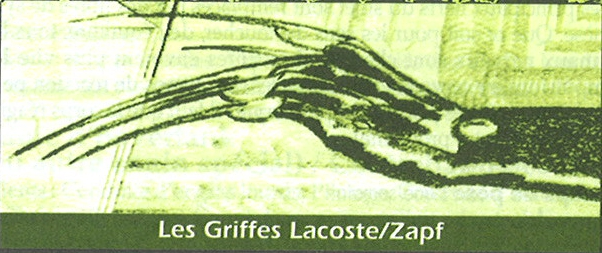
\includegraphics[width=0.45\textwidth]{img/griffesLacosteZapf.jpg} \end{center}

\textbf{M{\'e}taGriffes}~\\
On pose {\`a} la place des ongles des microplaques en c{\'e}ramique. Elles sont extr{\^e}mement fines (moins de deux millim{\`e}tres d'{\'e}paisseur repli{\'e}es). Elles de d{\'e}tendent avec un coup sec de la main, mettant les plaques les unes {\`a} la suite des autres, allongeant les ongles de 10 {\`a} 15cm. ~\\
La main est aussi {\'e}quip{\'e}e d'un c{\^a}blage qui permet trois types d'action : 
\begin{itemize}
	\footnotesize
	\item[$\bullet$] Faire passer des microcourants dans les M{\'e}taGriffes qui transforment la nature de la c{\'e}ramique (il s'agit d'un compos{\'e} biom{\'e}tallique dont la structure cristalline peut changer). Elles peuvent donc {\^e}tre tranchantes et dures comme un acier effil{\'e}, plus coupantes qu'un rasoir mais peu solides, et enfin peu tranchantes mais extr{\^e}mement solides. 
	\item[$\bullet$] T{\'e}taniser les muscles et les articulations de la main pour la rendre rigide (et donc permettre de donner des coups sans se rompre des os fragiles). 
	\item[$\bullet$] D{\'e}sactiver la <<soudure>> entre les plaques de c{\'e}ramique et permettre de replier avec pr{\'e}caution les M{\'e}taGriffes. 
\end{itemize}

Les r{\'e}glages se font en touchant certaines zones sensibles du poignet. ~\\
{\small 
	\textbf{Prix : }15 000\euro ~la main. ~\\
	\textbf{Temps de pose : }une heure, perte de 1 EP (Action). ~\\
	\textbf{Effets : }d{\'e}g{\^a}ts des M{\'e}taGriffes de [F]PV (mais cassure sur double-6 \emph{/ {\'e}chec critique}) ou bien de [c]PV et [D]PS ; tout en ayant une force normale. ~\\
	\textbf{Options : } un c{\^a}ble peut relier la main au cerveau, activant ainsi les fonctions par la pens{\'e}e. \textbf{Surco{\^u}t : } 3 000\euro . \textbf{Temps de pose : }3 heures. S'il y a d{\'e}j{\`a} un autre c{\^a}blage entre la main et le cerveau, on peut s'en servir sans en rajouter un autre. ~\\
} % \small

\textbf{Griffes}~\\
Les adolescents utilisent souvent des griffes non c{\^a}bl{\'e}es. Il s'agit simplement de grands ongles en acier souple, que l'on colle (de fa\c{c}on temporaire) aux derni{\`e}res phalanges. Ces griffes sont peu pratiques, peu efficaces mais donnent un <<look>> certain {\`a} leur possesseur. Il ne s'agit bien s{\^u}r pas d'un c{\^a}blage. ~\\
{\small 
	\textbf{Prix : }200\euro . ~\\
	\textbf{D{\'e}g{\^a}ts : }[D]PV, mais tout {\'e}chec avec une marge de 2 ou plus indique que les Griffes se sont d{\'e}tach{\'e}es ou que le poignet de l'aggresseur s'est cass{\'e} sous le choc. ~\\
} % \small

\textbf{{\'E}jecteur}~\\
Implantation d'une micro-cartouche {\`a} gaz dans la langue du patient, lui permettant de <<cracher>> une substance plus ou moins toxique sur son adversaire (technique dite du cobra). La port{\'e}e est de quatre m{\`e}tres maximum. Il faut juste faire attention \c{c} bien tirer la langue, {\`a} la coincer entre ses dents pour activer la capsule, et {\`a} ne pas ing{\'e}rer soi-m{\^e}me d produit. Le mod{\`e}le standard n'est pas consid{\'e}r{\'e} comme un c{\^a}blage et ne provoque aucune perte d'EP. ~\\
{\small 
	\textbf{Prix : }3 000\euro . ~\\
	\textbf{Temps de pose : }30 minutes. ~\\
	\textbf{Effets : }D{\'e}pend de la substance projet{\'e}e (poison, neurotoxique, etc. ). ~\\
	\textbf{Options : }Possibilit{\'e} d'activation par la pens{\'e}e. \textbf{Surco{\^u}t : } 2 000\euro . \textbf{Temps de pose : }1 heure. Cela deviens un vrai c{\^a}blage. %% ~\\
} ~\\

%% \vfill
%% \columnbreak

\textbf{Membre artificiel}~\\
Il s'agit de remplacer un ou plusieurs membres du patient par une version synth{\'e}tique en carbone et c{\'e}ramique. Avantages de l'op{\'e}ration : une plus grande r{\'e}sistance du membre, son insensibilit{\'e} aux variations de temp{\'e}rature ou d'atmosph{\`e}re, une plus grande force de frappe et de prise. Grave d{\'e}faut : beaucoup moins de pr{\'e}cision et de rapidit{\'e}. Si on peut faire des bras et des jambes acceptables, il est impossible de fabriquer une main artificielle aussi efficace qu'une vrai main. ~\\
{\small 
	\textbf{Prix : }{\`a} partir de 5 000\euro ~mais peut aller {\`a} plus d'un million suivant la qualit{\'e} et son apparence plus ou moins humaine. ~\\
	\textbf{Temps de pose : }1 jour {\`a} 1 semaine. ~\\
	\textbf{Effets : }Perte de 1 EP (Action). Malus de -1 \emph{(-10\%)} sur les tests faisant intervenir la pr{\'e}cision ou la rapidit{\'e} du membre en question (-2 \emph{(-20\%)} pour les mod{\`e}les bas de gamme). Bonus de +1 \emph{(+10\%)} sur les tests faisant intervenir la force. Le membre a une r{\'e}sistance allant de 3 {\`a} 6 Points de Structure. Un Point de Structure est perdu pour 1 PV ou 2 PS re\c{c}us. Un coup donn{\'e} avec la proth{\`e}se fait [B]PV et [D]PS de d{\'e}g{\^a}ts. ~\\
} % \small

\textbf{Yeux artificiels}~\\
Les yeux sont des organes facilement remplac{\'e}s. De plus, leur volume permet d'y loger facilement de l'{\'e}lectronique et de l'informatique, ce qui est plus difficile sous la peau ou dans le cr{\^a}ne. Ils peuvent {\^e}tre faits {\`a} la ressemblance d'yeux normaux, fluorescents... toutes les extravagances de la mode sont possibles. Le \textbf{temps de pose} est de deux heures, \textbf{sans convalescence}, {\`a} part quelques migraines et des ph{\'e}nom{\`e}nes de taches devant les yeux. Toute pose entra{\^i}ne la perte standard de 1 EP (Perception). ~\\
Mod{\`e}les standards : 
\begin{itemize}
	\footnotesize
	\item[$\bullet$] Infrarouge. Permet de d{\'e}tecter les sources de chaleur. \textbf{Prix : }7 000\euro . 
	\item[$\bullet$] Amplificateur d'image. Permet de b{\'e}n{\'e}ficier d'une analyse d'image plus pouss{\'e}e, comme une photo que l'on pourrait ensuite consulter avec une loupe. On peut stocker trente-six images diff{\'e}rentes. \textbf{Prix : }6 000\euro . 
	\item[$\bullet$] T{\'e}l{\'e}objectif. Comme son nom l'indique, permet de voir beaucoup plus loin qu'un \oe il humain classique (entre 3 et 5 km dans de bonnes conditions). \textbf{Prix : }9 000\euro . 
	\item[$\bullet$] Radar. Capte les {\'e}chos radars des objets m{\'e}talliques dans un rayon de 5 km autour du sujet et les transmet {\`a} son syst{\`e}me oculaire pour analyse. \textbf{Prix : }10 000\euro . 
	\item[$\bullet$] Lumi{\`e}re faible. Permet de voir la nuit avec tr{\`e}s peu de luminosit{\'e}. . \textbf{Prix : }5 500\euro . 
\end{itemize}
{\small 
	\textbf{Options : }on peut avoir un \oe il artificiel avec plusieurs des fonctions d{\'e}crites ci-dessus. Pour calculer son co{\^u}t ; additionner les prix et multiplier par le nombre de fonctions. Il est possible de polariser la surface de l'\oe il, pour le rendre insensible {\`a} une lumi{\`e}re aveuglante. Surco{\^u}t : 3 000\euro . Enfin, on peut connecter l'\oe il {\`a} une broche de type C pour pr{\'e}lever des images ou en envoyer {\`a} l'\oe il. Surco{\^u}t (en plus de la broche) : 1 000\euro . %% ~\\
} ~\\

\textbf{C{\^a}blage d'acquisition de cible}~\\
Il s'agit d'un c{\^a}ble qui relie un \oe il artificiel avec vis{\'e}e avec une arme sp{\'e}cifique. L'\oe il peut recevoir d'autres fonctions (voir ci-dessus). En version de base, l'\oe il est {\'e}quip{\'e} d'un micro{\'e}metteur et l'arme d'un r{\'e}cepteur pour les synchroniser. ~\\
{\small 
	\textbf{Prix : }6 000\euro ~pour l'\oe il, plus le prix de l'arme, ou 3 000\euro ~pour {\'e}quiper une arme quelconque. ~\\
	\textbf{Adaptation : }il faut r{\'e}gler antre l'\oe il et l'arme, et donc faire une s{\'e}ance de tir de deux heures. Si on change d'arme, il faut refaire le r{\'e}glage. De plus, ce type de <<c{\^a}blage>> fait perdre 2 EP (Action et Perception). ~\\
	\textbf{Temps de pose : }2 heures~\\
	\textbf{Effets : }on peut c{\^a}bler l'\oe il avec une broche de type C et ainsi mettre un caillou qui stockera les caract{\'e}ristiques de 256 armes diff{\'e}rentes. \textbf{Surco{\^u}t : }(en plus de la broche) 1 000\euro . On peut surtout faire courir un c{\^a}ble depuis l'\oe il jusqu'{\`a} la paume de la main qui tire. Ce qui {\'e}vite d'{\'e}ventuelles interf{\'e}rences radio. \textbf{Surco{\^u}t : }3 000\euro . \textbf{Temps de pose : }5 heures. \textbf{Convalescence : }bras inutilisable pendant 24 heures. ~\\
	\textbf{Options : }bonus de +2 au tir. Avec un c{\^a}blage musculaire, bonus suppl{\'e}mentaire de +1. Avec un c{\^a}blage nerveux, bonus suppl{\'e}mentaire de +1. Tous les bonus sont cumulatifs (en plus des bonus de connaissance des armes). ~\\
} % \small

\textbf{C{\^a}blage cam{\'e}ra}~\\
L'\oe il artificiel est reli{\'e} {\`a} un {\'e}metteur pos{\'e} sous la peau {\`a} la base du cr{\^a}ne, une antenne courant le long de la colonne vert{\'e}brale. L'{\'e}mission peut {\^e}tre faite en direction d'un proche relais terrestre ou d'un satellite. ~\\
{\small 
	\textbf{Prix : }de 3 000 {\`a} 100 000 \euro ~suivant la qualit{\'e} d'image, plus 10 000\euro ~pour l'{\'e}metteur. %% ~\\
	\textbf{Temps de pose : }6 heures~\\
	\textbf{Options : }on peut se passer d'un \oe il {\'e}lectronique en pontant sur la nerf optique, mais la qualit{\'e} d'image est moyenne (mais auquel cas il n'y a pas de perte d'{\'E}quilibre Psychique puisque l'op{\'e}r{\'e} ne sent aucune modification de son comportement normal). Enfin, on peut connecter l'\oe il {\`a} une broche de type C pour pr{\'e}lever des images et les enregistrer directement sur un magn{\'e}toscope externe. \textbf{Surco{\^u}t : }(en plus de la broche) 1 000\euro . ~\\
} % \small

\textbf{C{\^a}blage audio}~\\
De la m{\^e}me fa\c{c}on que l'on remplace un \oe il, on peut remplacer un conduit auditif ou lui envoyer des signaux divers. L'intervention dure une heure. Il n'y a pas d'adaptation (juste la perte de 1 EP -- Perception). Les diverses fonctions possibles sont : %% ~\\
\begin{itemize}
	\footnotesize
	\item[$\bullet$] R{\'e}seau t{\'e}l{\'e}phonique. Une mini antenne permet au personnage de se brancher automatiquement sur le circuit t{\'e}l{\'e}phonique o{\`u} qu'il se trouve dans le monde. ~\\
		\textbf{Prix : } 1 500\euro . 
	\item[$\bullet$] Scanner radio. Dispositif permettant d'{\'e}couter les liaisons radios et autres dans un rayon de 5 km. \textbf{Prix : } 1 200\euro . 
	\item[$\bullet$] D{\'e}tecteur {\'e}lectronique. Permet de d{\'e}tecter toute activit{\'e} {\'e}lectronique (micro, syst{\`e}mes d'alarmes, etc. ) dans un rayon de 300 m. \textbf{Prix : } 8 000\euro . 
	\item[$\bullet$] Talkie-Walkie. Pour communiquer {\`a} distance avec d'autres personnes, {\`a} condition qu'elles soient {\'e}quip{\'e}es. Sub-vocalisation pour envoyer des messages. \textbf{Prix : } 2 000\euro . 
\end{itemize}
{\small 
	\textbf{Options : }on peut avoir un c{\^a}blage avec plusieurs des fonctions ci-dessus. Pour calculer son co{\^u}t : additionner les prix, puis multiplier par le nombre de fonctions. ~\\
} % \small

\textbf{C{\^a}blage magn{\'e}tophone}~\\
	L'oreille es reli{\'e}e {\`a} un {\'e}metteur pos{\'e} sous la peau {\`a} la base du cr{\^a}ne, une antenne courant le long de la colonne vert{\'e}brale. L'{\'e}mission peut {\^e}tre faite en direction d'un proche relais terrestre ou d'un satellite. ~\\ 
{\small 
	\textbf{Prix : }7 000\euro ~pour l'{\'e}metteur. ~\\
	\textbf{Temps de pose : }6 heures~\\
	\textbf{Options : }on peut poser une oreille artificielle de meilleure qualit{\'e} (entre 3 000 et 6 000\euro ). Enfin, on peut connecter une broche de type C pour enregistrer directement sur un magn{\'e}tophone externe. \textbf{Surco{\^u}t : }(en plus de la broche) 1 000\euro . ~\\
} % \small

%% \barreCyberAgeHalf ~\\

\textbf{C{\^a}blage Matrice}~\\
On peut aller dans la Matrice sans aucun c{\^a}blage. Mais il faut alors poser des {\'e}lectrodes sur le cr{\^a}ne et la rapidit{\'e} des d{\'e}placements en Interface s'en ressent (voir plus loin) Les vrais Jackeurs pr{\'e}f{\`e}rent donc se c{\^a}bler en cons{\'e}quence. ~\\
La premi{\`e}re solution est de se faire poser une plaque : sorte de broche de type C (voir plus haut) et de se relier {\`a} une console d'Interface. \emph{(Voir {\'e}galement le prix des consoles dans la partie sur la Matrice. )} La seule diff{\'e}rence entre une plaque et ne broche est la qualit{\'e} des composants (or, argent, platine) et le fait qu'elle re\c{c}oit ET envoie des ordres (perte de 2 EP -- Action et Perception). 
La deuxi{\`e}me solution consiste {\`a} implanter l'{\'e}lectronique de la console dans la broche et sous le cr{\^a}ne. L'avantage est d'acc{\'e}l{\'e}rer encore le processus. Mais il faut toujours se relier {\`a} une borne informatique. {\small \textbf{Co{\^u}t : }8 000\euro , plus le prix de la console {\'e}quivalente multipli{\'e} par trois. \textbf{Temps de pose : }6 heures. } ~\\
La meilleure solution consiste {\`a} ajouter une liaison satellite autonome. Auquel cas un jackeur peut <<entrer en transe>> n'importe o{\`u} et se connecter {\`a} la Matrice. {\small \textbf{Surco{\^u}t : }12 000\euro . \textbf{Temps de pose : }8 heures. \textbf{Convalescence : }dos douloureux pendant 48 heures. }~\\

\textbf{Inhibiteurs}~\\
On peut c{\^a}bler les r{\'e}cepteurs du syst{\`e}me nerveux pour inhiber certains r{\'e}flexes. Par exemple la douleur, la faim, la fatigue. Dans chaque cas, cela implique une dur{\'e}e {\`a} ne pas d{\'e}passer et un temps de r{\'e}cup{\'e}ration de l'organisme une fois l'effort effectu{\'e}. Au meneur de jeu de g{\'e}rer comme il l'entend ce type de c{\^a}blage (perte de 1 EP par Perception, mais pertes temporaires {\'e}galement {\`a} chaque usage). ~\\

\textbf{Timbres}~\\
Le moyen le moins on{\'e}reux pour augmenter ses capacit{\'e}s physiques est le timbre appliqu{\'e} {\`a} m{\^e}me la peau. On utilise une dose d'endomorphine pour contrer la douleur, l'endoadr{\'e}naline pour augmenter les r{\'e}flexes ou encore l'endospeed pour augmenter les capacit{\'e}s musculaires. Malheureusement un timbre ne fonctionne que pour une dur{\'e}e limit{\'e}e (entre 5 et 10 minutes) et renouveler une prise plus d'une fois par 24 heures peux s'av{\'e}rer dangereux, le syst{\`e}me nerveux est satur{\'e} et c'est l'accident. ~\\
{\small 
	\textbf{Prix : }50 {\`a} 2 000\euro ~la dose suivant le produit. ~\\
	\textbf{Effets : }bonus de +1 lorsque c'est applicable. Ensuite toutes les actions du m{\^e}me type {\`a} -2 pendant deux heures. Si on prend plusieurs doses en moins de 24 heures, faire un test Corps~\imgCORPS + R{\'e}sistance~\imgRESIS + Humain~\imgHUMAI avec comme malus le nombre de doses. En cas d'{\'e}chec, coma imm{\'e}diat de douze heures. ~\\
} % \small

\barreCyberAgeHalf ~\\

%% \vfill ~\\
%% \columnbreak

\textbf{G.O.S.T.}~\\
Groupe Op{\'e}ratoire de Survie Test. C'est un ensemble de capteurs diss{\'e}min{\'e}s dans tous le corps, qui testent les diff{\'e}rents param{\`e}tres de survie d'un sujet et donnent l'alarme lorsqu'un param{\`e}tre vient {\`a} baisser. L'alerte peut {\^e}tre visuelle, si le sujet a un \oe il artificiel, sinon elle est sonore (c{\^a}bl{\'e}e dans le conduit auditif). ~\\
{\small 
	\textbf{Prix : }95 000\euro . ~\\
	\textbf{Temps de pose : }une semaine. Perte de 1EP (Perception). ~\\
} % \small

\textbf{G.O.S.T. de combat}~\\
C'est un mod{\`e}le qui permet d'injecter au moment appropri{\'e} des drogues ou des m{\'e}dicaments au personnage pour le maintenir en {\'e}tat d'alerte, ou le faire survivre. Des microvalves peuvent arr{\^e}ter des h{\'e}morragies, etc. Perte de 1 EP (Perception et R{\'e}sistance). ~\\
{\small 
	\textbf{Prix : }350 000\euro . ~\\
	\textbf{Temps de pose : }1 mois. ~\\
	\textbf{Effets : }possibilit{\'e} d'avoir un membre du corps {\`a} 0 ou -1 PV sans qu'il soit perdu. Quadruple le temps durant lequel le corps peut survivre en attendant l'op{\'e}ration. {\'E}limine la majorit{\'e} des effets des poisons et des gaz toxiques. Permet un taux de r{\'e}cup{\'e}ration de 1 PV par jour sans soins autres que ceux du G.O.S.T. R{\'e}cup{\'e}ration de 1 PS par quart d'heure. Il faut recharger le G.O.S.T. apr{\`e}s chaque grande d{\'e}pense de composantes (plauqe de r{\'e}serve entre les omoplates du patient). ~\\
} % \small	

\barreCyberAgeHalf ~\\

\textbf{C{\^a}blage total}~\\
Plut{\^o}t que d'ajouter au fur et {\`a} mesure des {\'e}quipements cybern{\'e}tiques, ce qui risque de poser des probl{\`e}mes de compatibilit{\'e}, et augmente les probabilit{\'e}s de maladresse chirurgicale, certains mercenaires optent d'embl{\'e}e pour le c{\^a}blage total. Celui-ci consiste en un c{\^a}blage nerveux de vitesse, un c{\^a}blage musculaire, le remplacement des yeux et des oreilles par des proth{\`e}ses standards, un c{\^a}blage du cerveau {\'e}quivalent {\`a} une broche de type C et deux broches de type B, une antenne satellite le long de la colonne vert{\'e}brale, des <<c{\^a}bles>> courant sous tous les membres, un G.O.S.T. de combat et enfin une mini-centrale informatique pour g{\'e}rer le tout. ~\\
En bref, un individu ainsi c{\^a}bl{\'e} peut se faire rajouter sans aucun probl{\`e}me n'importe quel autre {\'e}quipement cybern{\'e}tique, et cela avec le minimum de chirurgie. Perte de 3 EP (Action, Perception et R{\'e}sistance), plus une d{\'e}pense en Points de R{\`e}gnes et / ou {\'E}nergies {\'e}gale {\`a} 7. ~\\
{\small 
	\textbf{Prix : }600 000\euro . ~\\
	\textbf{Temps de pose : }2 mois~\\
	\textbf{Adaptation : }voir les autres c{\^a}blages plus haut. ~\\
	\textbf{Effets : }voir les autres c{\^a}blages plus haut. ~\\
} % \small

%% \barreCyberAgeHalf ~\\
%% \vfill ~\\
\columnbreak

\textbf{Interfacer broches et syst{\`e}mes c{\^a}bl{\'e}s}~\\
Pour une efficacit{\'e} totale, on peut interfacer un caillou avec un c{\^a}ble. Un tel syst{\`e}me permet un bonus automatique de +8 \emph{(+60 {\`a} +80\%)} si l'on agit dans un cadre de non-urgence. Ce genre d'interface peut marcher pour un chirurgien, un pianiste, etc. Il permet une ex{\'e}cution sans faille de proc{\'e}dures normales (et m{\^e}me {\`a} grande vitesse). Mais il ne permet pas l'improvisation, l'adaptation {\`a} des cas non pr{\'e}vus. ~\\
Exemple : Georges Jacques s'est fait c{\^a}bler les nerfs et les muscles des doigts. Et il poss{\`e}de une broche avec un caillou expliquant comment forcer des coffres. Autant dire que la porte du coffre mod{\`e}le standard qui est devant lui s'ouvre sans mal en moins de 30 minutes. %% ~\\

%% \barreCyberAgeHalf ~\\

\begin{center} 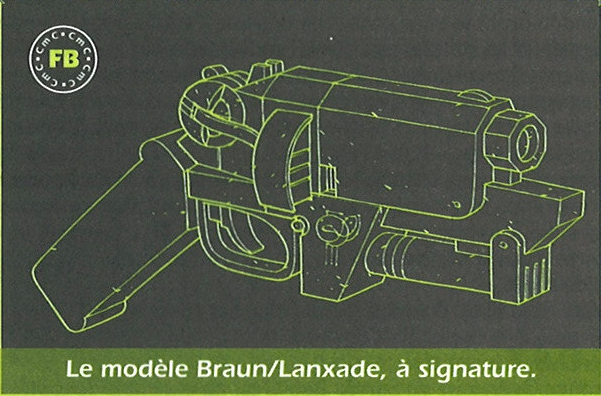
\includegraphics[width=0.43\textwidth]{img/armeSignatureBraunLanxade.jpg} \end{center}

%% \textbf{\large Les armes}~\\
\subsubsection*{Les armes\markboth{Les armes}{Les armes}}
\addcontentsline{toc}{subsubsection}{Les armes}
En plus des classiques armes {\`a} feu qui n'ont que tr{\`e}s l{\'e}g{\`e}rement {\'e}volu{\'e}es, il existe quelques nouvelles classes d'armes. %% ~\\

\textbf{Les armes intelligentes}~\\
Il s'agit d'une nouvelle g{\'e}n{\'e}ration d'armes {\`a} feu. L'arme en tant que telle ne change pas mais elle est reli{\'e}e {\`a} un ordinateur de cible coupl{\'e}e {\`a} une vis{\'e}e laser. L'arme se <<bloque>> sur une cible et quand on la suit, ne d{\'e}clenche le tir que s'il y a <<acquisition>> de la cible. Cons{\'e}quence : malus de -1 ou -2 au tir instinctif au lieu de -2 {\`a} -4. Et bonus au test de tir normal de +2. Le tout est cumulable avec un c{\^a}blage d'acquisition de cible (voir plus haut). ~\\
\textbf{Prix : }entre 3 000 et 15 000\euro ~suivant l'arme. ~\\
\textbf{D{\'e}g{\^a}t : } ~\\

\textbf{Armes monofilament, composites}~\\
Toutes les armes blanches normales peuvent {\^e}tre travaill{\'e}es pour {\^e}tre rendues plus tranchantes, plus efficaces. Pour les d{\'e}g{\^a}ts, il suffit de prendre la cat{\'e}gorie de l'arme et de la d{\'e}placer de deux colonnes {\`a} droite \emph{-- +1D6 {\`a} +2D6 -- } (pour les PV seulement). Quand on fait un double-6 \emph{({\'e}chec critique)} avec une telle arme, elle perd son tranchant et perd {\`a} chaque fois une colonne de d{\'e}g{\^a}ts (jusqu'{\`a} devenir moins bonne qu'une arme traditionnelle). Exemple : Un katana normal fait [F]PV et [A]PS, un katana avec son tranchant trait{\'e} fera [h]PV et [A]PS. ~\\
Il existe quelques armes exp{\'e}rimentales qui d{\'e}calent les d{\'e}g{\^a}ts de quatre colonnes \emph{(+4D6 de d{\'e}g{\^a}ts)}, et ne font plus aucun PS tellement elles sont tranchantes (un katana ainsi trait{\'e} ferait [j]PV). Mais leur fragilit{\'e} les fait se briser sur tout double aux d{\'e}s. ~\\
\textbf{Prix : }prix de l'arme normale multipli{\'e} par quatre. En g{\'e}n{\'e}ral de 8 000 {\`a} 15 000\euro . ~\\
\textbf{D{\'e}g{\^a}t : }plus deux colonnes pour les PV \emph{(+2D6)}. ~\\

\textbf{Fouet monofilament}~\\
Ce fouet d'un seul tenant, sorte de c{\^a}ble d'acier extrafin, est capable de d{\'e}couper m{\^e}me de l'acier si on l'utilise avec suffisamment de force. Seul probl{\`e}me : son maniement est tr{\`e}s d{\'e}licat. ~\\
Le talent de base est {\`a} -4 \emph{(10-20\%)}. Tant que l'on est pas au niveau 0 \emph{(50\%)}, tout double aux d{\'e}s, m{\^e}me en cas de test de combat r{\'e}ussi, am{\`e}ne une maladresse \emph{({\'e}chec critique)}. La maladresse est simple : l'utilisateur du fouet s'en prend un coup sur une partie du corps, au hasard. Les d{\'e}g{\^a}ts se calculent normalement avec la ME (Marge d'{\'E}chec {\`a} la place de la MR (Marge de R{\'e}ussite) si c'est un {\'e}chec, et la MR {\`a} 0 si cela avait {\'e}t{\'e} un <<{\'e}chec>>. {\`A} partir du niveau 0 \emph{(50\% et plus)}, seul le double-6 \emph{({\'e}chec critique)} est toujours une maladresse. ~\\ 
\textbf{Prix : }800\euro . ~\\
\textbf{D{\'e}g{\^a}t : }[H]PV. ~\\

\textbf{Vibrodague}~\\
Il s'agit d'une dague vibrante, en mat{\'e}riaux composites. Elle peut d{\'e}couper des m{\'e}taux ou du bois comme une mini-tron\c{c}onneuse. Elle est aussi tr{\`e}s dangereuse au corps {\`a} corps. ~\\
\textbf{Prix : }1 500\euro . Pile (2 heures d'utilisation) 200\euro . ~\\
\textbf{D{\'e}g{\^a}t : }[F]PV et [C]PS. ~\\

\textbf{Pistolet {\`a} fl{\'e}chette}~\\
Principalement d{\'e}velopp{\'e}es pour les forces op{\'e}rant dans l'espace (car les armes {\`a} feu courantes sont dangereuses m{\^e}me pour l'utilisateur dans cet environnement), les armes {\`a} fl{\'e}chettes n'en sont pas moins redoutables. Les fl{\'e}chettes peuvent contenir toute une panoplie de syst{\`e}mes d'armes allant d'un poison ultra rapide {\`a} un puissant anesth{\'e}siant. ~\\
\textbf{Prix : }1 300\euro ~plus fl{\'e}chettes. ~\\
\textbf{D{\'e}g{\^a}t : }variable selon le contenu de la fl{\'e}chette. ~\\

\textbf{Pistolet {\'e}lectrique (taser)}~\\
Second syst{\`e}me d'arme d{\'e}coulant de l'espace et ayant fait son apparition sur Terre, les tasers sont l'arme favorite des forces de police spatiales, elles ont l'avantage de pouvoir arr{\^e}ter net un assaillant sans le blesser gravement. ~\\
\textbf{Port{\'e}e : }15 m{\`e}tres. ~\\
\textbf{Prix : }4 000\euro . ~\\
\textbf{D{\'e}g{\^a}t : }mod{\`e}le courant [I]PS, mod{\`e}le des forces de police : [A]PV et [J]PS. %% ~\\

\textbf{Armes {\`a} Tr{\`e}s Basses Fr{\'e}quences}~\\
Ce sont des diffuseurs d'ondes infrasonores. Tout homme dans le rayon d'action des armes (cela d{\'e}pend du mod{\`e}le) doit r{\'e}ussir un test Corps~\imgCORPS + R{\'e}sistance~\imgRESIS + Humain~\imgHUMAI -6 pour ne pas se tordre de douleur. Tout le monde subit une perte de [B+3]PS. Si l'{\'e}mission dure plus de 20 minutes, tout personnage qui ne r{\'e}ussit pas un test Corps~\imgCORPS + R{\'e}sistance~\imgRESIS + Humain~\imgHUMAI subit une perte de 2PS pour les prochaines 24 heures. Une nanoarmure donne un bonus de +4 {\`a} ces tests. %% ~\\

%% \barreCyberAgeHalf ~\\

%% \textbf{\large Armures}~\\
\subsubsection*{Armures\markboth{Armures}{Armures}}
\addcontentsline{toc}{subsubsection}{Armures}
M{\^e}me si la technologie des armures a {\'e}volu{\'e}, peu de gens en portent encore, m{\^e}me en zone de combat. En effet, les armes sont tellement mortelles que les armures apportent une protection d{\'e}risoire. %% ~\\

\textbf{Armures c{\'e}ramiques}~\\
Ce sont des armures qui absorbent tr{\`e}s peu les coups mais les d{\'e}vient particuli{\`e}rement bien, et ne sont pas trop g{\^e}nantes; Elles sont du type 4/1/0. ~\\
C'est-{\`a}-dire que m{\^e}me en cas de succ{\`e}s, votre adversaire doit faire au moins une marge de r{\'e}ussite de 4 pour vous toucher (son test est diminu{\'e} de 4). Tous vos tests ont une valeur diminu{\'e}e de 1. {\`A} chaque fois qu'un coup passe, la protection est diminu{\'e}e de 1. ~\\
\textbf{Prix : }le prix est d'environ 5 000\euro ~pour une armure sur le haut du corps et casque, de 8 000\euro ~pour une couverture totale. ~\\

\textbf{NanoArmures}~\\
Au contraire, les nanoarmures sont l{\`a} pour absorber les chocs, et sont particuli{\`e}rement efficaces pour les d{\'e}g{\^a}ts de souffle. Une nanoarmaure doit r{\'e}guli{\`e}rement {\^e}tre r{\'e}g{\'e}n{\'e}r{\'e}e avec un mat{\'e}riel sp{\'e}cial. ~\\
Elles apportent une protection de 0/0/6, 0/1/8 ou 0/3/12 suivant les mod{\`e}les (le dernier mod{\`e}le, trois fois plus chet, est r{\'e}serv{\'e} aux pilotes de chars, qui n'ont pas besoin d'une grande mobilit{\'e}). D{\`e}s que le porteur subit un coup tranchant (perte de 1 PV ou plus) la nanoarmure ne fonctionne plus (et vaut alors 0/0/0, 0/1/0 ou 0/4/0) et n'est plus reg{\'e}n{\'e}rable. D{\`e}s que la victime subit 1 PS ou plus (d{\'e}g{\^a}ts de souffle), la nanoarmure perd 1 point de protection d'absorption mais elle est (et reste) reg{\'e}n{\'e}rable. ~\\
\textbf{Prix : }10 000\euro . ~\\
\textbf{Reg{\'e}n{\'e}ration : }1 000\euro ~(en une heure de bain de reconstruction). ~\\

\barreCyberAgeHalf ~\\

 %% \vfill
 %% \columnbreak

%% \textbf{\Large Personnages pr{\'e}-tir{\'e}s -- SimulacreS}~\\
\subsection*{Personnages pr{\'e}-tir{\'e}s -- SimulacreS\markboth{Personnages pr{\'e}-tir{\'e}s -- SimulacreS}{Personnages pr{\'e}-tir{\'e}s -- SimulacreS}}
\addcontentsline{toc}{subsection}{Personnages pr{\'e}-tir{\'e}s -- SimulacreS}

\emph{Voir pages suivantes... Biographies et fiches d{\'e}taill{\'e}es pour \emph{SimulacreS} et \emph{Basics} (syst{\`e}me du jeu de r{\^o}le de l'\emph{Appel de Cthullu}). }

\end{multicols*}

\clearpage

\subsubsection*{Biographies des personnages pr{\'e}-tir{\'e}s \emph{Cyber Age}\markboth{Biographies des personnages pr{\'e}-tir{\'e}s \emph{Cyber Age}}{Biographies des personnages pr{\'e}-tir{\'e}s \emph{Cyber Age}}}
\addcontentsline{toc}{subsubsection}{Biographies des personnages pr{\'e}-tir{\'e}s \emph{Cyber Age}}

\begin{multicols}{2}
	\footnotesize
	
	\textbf{Ernst Kobel}~\\
	Ernst devient pilote {\`a} la suite de son {\'e}viction d'un gang d'adolescents dans la banlieue de Sao Paulo. Il remporte de nombreuses courses et tombe amoureux d'une vedette du \texttt{CosmoR{\^e}ve} : Elisa M{\'e}tamorphosis. C'est {\`a} cette {\'e}poque qu'il se fait poser un c{\^a}blage de pilotage multifonctions Data System Sensei. ~\\
	S'apercevant que son amie devient peu {\`a} peu folle, il tente de racheter son contrat. Pour cela il c{\`e}de au \texttt{Yakuza} et accepte de truquer une course. Mais en voulant couper la route {\`a} un concurrent sa voile s'enflamme et c'est l'accident, il perd la vue. ~\\
	Des mois de convalescence passent, Elisa sombre dans la folie. Ernst abandonne la course et se fait poser des yeux {\'e}lectroniques Zeiss / Ikon. ~\\
	Il redescend sur Terre, star d{\'e}chue. Amateur de sensations fortes, il d{\'e}cide de devenir chasseur de primes. Gr{\^a}ce {\`a} d'anciens contacts, il apprend les rudiments du m{\'e}tier aupr{\`e}s de l'Agence new-yorkaise Mac Burns. Il s'est install{\'e} depuis peu {\`a} La D{\'e}fense. ~\\
	
	\textbf{Paul Morgan}~\\
	En 2066, Paul Morgan est victime du c{\'e}l{\`e}bre coup de main contre la navette Berlin-Tokyo perp{\'e}tu{\'e} par la \emph{neu-RAF}. Il a 15 ans, et cette m{\'e}saventure le marque. C'est sans doute {\`a} cause de cet incident qu'il d{\'e}cide de devenir \texttt{HoloReporter}. Sa vid{\'e}o sur les \texttt{gangs} de Hambourg lui vaut d'{\^e}tre engag{\'e} au \texttt{Network} \emph{NHK}. Il poursuit sa carri{\`e}re en sortant un reportage sur son exfiltration du \texttt{TechnoBloc} \emph{General Electric}, {\`a} la fronti{\`e}re du Mexique, qui lui vaut de devenir une r{\'e}f{\'e}rence dans son m{\'e}tier. Suivent des reportages sur les \texttt{Wampires}, les \texttt{BladeRunners} et les \texttt{Yakuzas}. ~\\
	Dans tous les cas, Paul s'arrange, contrairement {\`a} la pratique journalistique courante, pour se faire de nombreux amis, il prot{\`e}ge ses sources et ne cherche jamais le sensationnel. ~\\
	Il est toujours {\`a} la recherche d'un sujet et pr{\^e}t {\`a} prendre tous les risques pour le ramener, c'est un des rares exemples de journaliste honn{\^e}te et consciencieux. ~\\
	
	\textbf{Jenel Astaki}~\\
	{\`A} 18 ans, Jenel tue un \texttt{Yakuza}, dans des circonstances mal {\'e}lucid{\'e}es, dans un {\'e}cosyst{\`e}me d'\emph{Atlantide III} (une \texttt{Venise} au large de la Floride) d'o{\`u} il est originaire : il a des g{\`e}nes \texttt{Triton} modifi{\'e}s. Pour {\'e}chapper {\`a} la vengeance du gang, il signe un contrat de mineur en \texttt{Espace Profond}. Il y fait la connaissance d'un ancien \texttt{Jackeur} retir{\'e} qui lui donne quelques tuyaux en {\'e}change d'une protection. Il tente une passe contre une base de donn{\'e}es du \texttt{TechnoBloc} \emph{Avant Garde} {\`a} partir de l'ast{\'e}ro{\"i}de \emph{Alpha V}. Pour cela, faisant confiance {\`a} un autre <<transform{\'e}>>, il s'adjoint les services d'un \texttt{Phase II} qui doit assurer une op{\'e}ration de diversion. Mais le \texttt{Phase II} n'est pas au rendez-vous et Jenel manque de se faire pi{\'e}ger par un programme tueur \emph{Janissaire}. ~\\
	Fuyant dans une navette, le syst{\`e}me de propulsion se met en panne et il reste un an en \texttt{Synthivers} avant d'{\^e}tre r{\'e}cup{\'e}r{\'e} par un cargo non loin de Mars. Les quatre ann{\'e}es suivantes, il rembourse les frais de sauvetage en travaillant comme \texttt{CyberTek} pour divers \texttt{TechnoBlocs}. Il vient de revenir sur Terre. ~\\
	Jenel est une t{\^e}te br{\^u}l{\'e}e, endurci par les mois pass{\'e}s en \texttt{Espace Profond}, rejet{\'e} aussi bien par les \texttt{Tritons} que par les \texttt{Nomades}. Il n'est anim{\'e} que par un objectif : retrouver le \texttt{Phase II} et le tuer. Mais pour cela, il faut repartir dans l'espace et \c{c}a co{\^u}te de l'argent, beaucoup d'argent. ~\\
	
	\vfill
	\columnbreak
	
	\textbf{Sandra Vitteker}~\\
	{\`A} 17 ans, Sandra blesse mortellement un \texttt{R{\^o}nin} dans une ruelle du vieux Londres, elle affirmera qu'il voulait la violer. Cette action d'{\'e}clat lui vaut d'{\^e}tre remarqu{\'e} par les \texttt{Yakuzas} qui lui font des propositions d'embauche. ~\\
	Durant deux ann{\'e}es, Sandra devient membre d'un gang \texttt{Yakuza} bas{\'e} {\`a} Paris. Son parrain lui paye un c{\^a}blage et une formation de Pilote de Voile Solaire. {\`A} 19 ans, elle participe {\`a} sa premi{\`e}re course mais abandonne rapidement, elle ne supporte pas de reste plus d'un mois seule dans l'espace. C'est {\`a} cette {\'e}poque qu'elle rencontre un \texttt{R{\^o}nin} avec qui elle se lie d'amiti{\'e} et qui lui apprend les trucs du m{\'e}tier. Il se fait malheureusement descendre. ~\\
	Sandra recommence {\`a} travailler pour son gang comme tueuse {\`a} gage et sauve la mise {\`a} un \texttt{BladeRunner} d{\'e}butant venu op{\'e}rer sur son territoire. Elle vient de quitter les \texttt{Yakuzas} pour travailler en free-lance, comme garde du corps. ~\\
	D'apr{\`e}s ses propres conclusions, <<elle n'est bonne que comme flingueuse>> et d'apr{\`e}s tous les avis, \c{c}a semble {\^e}tre effectivement le cas. ~\\
	
	\textbf{J{\'e}r{\'e}miah Steel}~\\
	J{\'e}r{\'e}miah passe son enfance dans les quartiers pauvres de Saint-Ouen. Bless{\'e} dans une bagarre entre gangs, il d{\'e}cide de lettre {\`a} profit sa convalescence pour apprendre aupr{\`e}s d'un ami les rudiment du m{\'e}tier de \texttt{Jackeur}. ~\\
	C'est l{\`a} qu'il rend un service inconnu {\`a} une I.A. bancaire des Cara{\"i}bes. Gr{\^a}ces aux b{\'e}n{\'e}fices tir{\'e}s de cette coop{\'e}ration, il entre au \texttt{TechnoBloc} \emph{Exxon} et se fait poser un c{\^a}blage d'Interface Nakamichi. Vers l'{\^a}ge de 19 ans, il a une liaison avec une dirigeante de son \texttt{TechnoBloc} qui se termine rapidement, les deux amants gardant de bons contacts. Trouvant sa vie trop fade, J{\'e}r{\'e}miah d{\'e}cide peu apr{\`e}s de s'engager dans les <<Maraudeurs de Merill>>, une \texttt{Force Mercenaire} de bon niveau. Il y entre directement comme officier gr{\^a}ce {\`a} sa formation de \texttt{Jackeur}. On lui pose une broche avec des cailloux de maniement d'armes. Un an apr{\`e}s son engagement, il est bless{\'e} lors d'une guerre priv{\'e}e \emph{ITT} conte \emph{Hoffman Laroche} en Californie du Sud. Apr{\`e}s plusieurs mois d'h{\^o}pital, il est lib{\'e}r{\'e} et garde de sa mission une impressionnante cicatrice au ventre. ~\\
	Sa prime en poche, il est disponible pour toute mission impliquant un peu d'action. Steel est un bon \texttt{Jackeur}, sans {\^e}tre un as ; il b{\'e}n{\'e}ficie d'une bonne formation militaire. C'est un aventurier qui ne tient pas en place, il aime l'action et le danger. ~\\
	
	\textbf{Irina Toss}~\\
	{\`A} 15 ans, Irina est prise pour cible dans une \texttt{Chasse}. Chose rare, c'est elle qui {\'e}limine son chasseur et cet exploit lui vaut d'{\^e}tre remarqu{\'e}e par le \texttt{Yakuza} qui lui propose une place de garde du corps dans un gang. Plus tard, ses activit{\'e}s lui attirent l'animosit{\'e} d'un \texttt{TechnoBloc} qui envoie un \texttt{BladeRunner} contre elle, un professionnel, que l'on retrouve avec une balle dans la t{\^e}te au fond d'une ruelle de Singapour. Gr{\^a}ce {\`a} ses contacts au sein du \texttt{Yakuza}, Irina gagne de coquettes sommes dans les paris sur les \texttt{Courses Solaires}. Plusieurs mois passent, elle se lie d'amiti{\'e} avec un certain David Feeshop, un \texttt{R{\^e}veur} professionnel et organise son exfiltration de l'\texttt{Usine {\`a} R{\^e}ves} de Toronto (appartenant au \texttt{TechnoBloc} \emph{MGM/Sony}). Arr{\^e}t{\'e}e {\`a} la suite de cette op{\'e}ration, elle refuse de collaborer avec les services de police du \texttt{TechnoBloc} qui lui proposent de livrer ses contacts \texttt{Yakuzas} contre une remise de peine. Elle {\'e}cope d'une condamnation de 3 ans dans les mines spatiales. Entre-temps, David a subi le sort des r{\^e}veurs professionnels : il d{\'e}ambule dans les couloirs d'un discret h{\^o}pital psychiatrique. ~\\
	Irina vient de terminer son temps et de revenir sur Terre. C'est une tueuse, lucide et froide, tr{\`e}s intelligente et sans un soup\c{c}on de piti{\'e}. ~\\

\end{multicols}

\clearpage

\subsubsection*{Personnages pr{\'e}-tir{\'e}s \emph{Cyber Age} -- SimulacreS\markboth{Personnages pr{\'e}-tir{\'e}s \emph{Cyber Age} -- SimulacreS}{Personnages pr{\'e}-tir{\'e}s \emph{Cyber Age} -- SimulacreS}}
\addcontentsline{toc}{subsubsection}{Personnages pr{\'e}-tir{\'e}s \emph{Cyber Age} -- SimulacreS}

\begin{longtable}[ht]{ p{0.99\textwidth} }
		\hline 
	\endfirsthead
		\hline
	\endhead
		\hline
	\endfoot
		\hline
	\endlastfoot
	\begin{tabular}[h]{ p{0.17\textwidth} p{0.47\textwidth} p{0.32\textwidth} }
		\textbf{Ernst Kobel}										\newline
		\textbf{\small Bladerunner, ancien pilote de voile solaire}	\newline
			\newline
		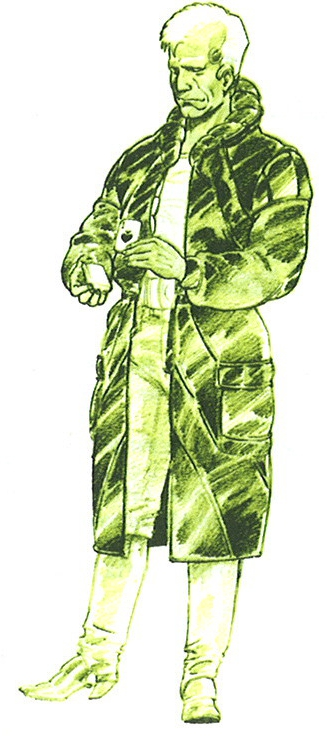
\includegraphics[width=0.15\textwidth]{img/personnageErnstKobel.jpg}
			\newline
		
		& %% first to second column of the first row of the personnae
			
		\textbf{{\'E}quipement cybern{\'e}tique : }C{\^a}blage optique infrarouge des deux yeux. C{\^a}blage de pilotage. Broche de Type A. \newline
		\textbf{Cailloux : }Pilotage de voile solaire. Pilotage d'hovertank. Anglais. Japonais. Fran\c{c}ais. \newline
		\textbf{{\^A}ge : } 28 ans 											\newline
		\textbf{Parrain : } --- 											\newline
		\textbf{Argent : } 800 \euro 										\newline
		\textbf{Divers : } ---												\newline
		\textbf{M{\'e}tier : } Pilote de voile solaire						\newline
		\textbf{Autres talents : } Filature 0 ; Combat {\`a} mains nues 0 ; Pistolet 0 ; Astrophysique -2. \newline
		
		%% \hline
		\textbf{{\'E}l{\'e}ments biographiques}
		\begin{itemize}
			\item[9/10] Dette vis {\`a} vis d'un Yakuza. 
			\item[12/3] Un R{\^e}veur devient fou. 
			\item[5/12] Une agence de d{\'e}tectives vous apprend les rudiments du m{\'e}tier de BladeRunner. 
			\item[3/7] Vous devenez Pilote de Voile Solaire
			\item[6/9] Accident. Perte des yeux. 
			\item[8/10] C{\^a}blage gratuit. 
		\end{itemize}
		
		& %% second to third column of the first row of the personnae
		
			{\centering \emph{Composantes}}	\newline
				{\footnotesize %
				\begin{tabular}[h]{|p{0.25cm}|p{3.00cm}|p{0.75cm}|}
					%% \begin{tabular}[c]{|p{0.05cm}|} \\ \hline \\ \hline \\ \end{tabular}
					\hline
					\imgCORPS & CORPS		&	5	\\
					\hline
					\imgINSTI & INSTINCT	&	6	\\
					\hline
					\imgCOEUR & C\OE UR		&	4	\\
					\hline
					\imgESPRI & ESPRIT		&	3	\\
					\hline
				\end{tabular} }
			\newline
			
			{\centering \emph{Moyens}} \newline
				{\footnotesize %
				\begin{tabular}[h]{|p{0.25cm}|p{3.00cm}|p{0.75cm}|}
					\hline
					%% \vspace{0.05pt} & & \\
					\imgPERCE &  PERCEPTION		 & 4 \\
					\hline
					%% \vspace{0.05pt} & & \\
					\imgACTIO &  ACTION			 & 3 \\
					\hline
					%% \vspace{0.05pt} & & \\
					\imgDESIR &  D{\'E}SIR		 & 2 \\
					\hline
					%% \vspace{0.05pt} & & \\
					\imgRESIS &  R{\'E}SISTANCE	 & 1 \\
					\hline
				\end{tabular} }
			\newline
			
			\begin{tabular}[h]{ p{4.0cm} }
				\emph{R{\^e}gnes}  \\
				{\footnotesize %
				\begin{tabular}[h]{|p{0.25cm}|p{1.50cm}|p{0.25cm}|p{1.50cm}|}
					\hline
					\imgMINER 	& Min{\'e}ral		\newline 0	 & \imgVEGET	& V{\'e}g{\'e}tal		\newline 0					\\
					\hline
					\imgANIMA 	& Animal			\newline 0	 & \imgHUMAI	& Humain				\newline 1					\\
					\hline
					\imgMECAN	& M{\'e}canique		\newline 2	 & \imgNEANT	& N{\'e}ant				\newline \textbf{-1}		\\ 
					\hline
				\end{tabular} } \\
				\\
				\emph{{\'E}nergies de base} \\
				{\footnotesize %
				\begin{tabular}[h]{|p{0.25cm}|p{1.50cm}|p{0.25cm}|p{1.50cm}|}
					\hline
					\imgPUISS	& Puissance			\newline 0	 & \imgRAPID	& Rapidit{\'e}			\newline 1				\\
					\hline
					\imgPRECI	& Pr{\'e}cision		\newline 1	 &				&												\\
					\hline
				\end{tabular} } \\
			\end{tabular}
			\newline \newline \newline 
			Points de Vie : 6			\newline
			Points de Souffle : 4		\newline
			{\'E}quilibre Psychique : 1	\newline 
		\\ %% end of first row of the personnae
		%% second row of the personnae
		%% \hline
		%% \multicolumn{3}{ p{0.98\textwidth} }{ \textbf{Description} }\\
		%% Ernst devient pilote {\`a} la suite de son {\'e}viction d'un gang d'adolescents dans la banlieue de Sao Paulo. Il remporte de nombreuses courses et tombe amoureux d'une vedette du \texttt{CosmoR{\^e}ve} : Elisa M{\'e}tamorphosis. C'est {\`a} cette {\'e}poque qu'il se fait poser un c{\^a}blage de pilotage multifonctions Data System Sensei. \newline
		%% S'apercevant que son amie devient peu {\`a} peu folle, il tente de racheter son contrat. Pour cela il c{\`e}de au \texttt{Yakuza} et accepte de truquer une course. Mais en voulant couper la route {\`a} un concurrent sa voile s'enflamme et c'est l'accident, il perd la vue. \newline
		%% Des mois de convalescence passent, Elisa sombre dans la folie. Ernst abandonne la course et se fait poser des yeux {\'e}lectroniques Zeiss / Ikon. \newline
		%% Il redescent sur Terre, star d{\'e}chue. Amateur de sensations fortes, il d{\'e}cide de devenir chasseur de primes. Gr{\^a}ce {\`a} d'anciens contacts, il apprend les rudiments du m{\'e}tier aupr{\`e}s de l'Agence new-yorkaise Mac Burns. Il s'est install{\'e} depuis peu {\`a} La D{\'e}fense. \newline
	\end{tabular} \newline \\
	
	
		\hline
	\begin{tabular}[h]{ p{0.17\textwidth} p{0.47\textwidth} p{0.32\textwidth} }
		\textbf{Paul Morgan}										\newline
		\textbf{\small Holoreporter}								\newline
			\newline
		\includegraphics[width=0.15\textwidth]{img/personnagePaulMorgan.jpg}		
			\newline
			
		& %% first to second column of the first row of the personnae
			
		\textbf{{\'E}quipement cybern{\'e}tique : }C{\^a}blage optique : enregistreur vid{\'e}o. C{\^a}blage auditif : t{\'e}l{\'e}phonique. \newline
		\textbf{{\^A}ge : } 29 ans 											\newline
		\textbf{Parrain : } Un ancien BladeRunner. 							\newline
		\textbf{Argent : } 12 000\euro 										\newline
		\textbf{Divers : } dette d'un Yakuza, dette envers un Wampire		\newline
		\textbf{M{\'e}tier : } Holoreporter									\newline
		\textbf{Autres talents : } Filature 0 ; Connaissance de la rue 0 ; Gestion 0 ; Chimie -2 ; Falsification de documents {\'e}crits -2 ; Danse 0. \newline
		
		%% \hline
		\textbf{{\'E}l{\'e}ments biographiques}
		\begin{itemize}
			\item[3/12] Victime d'une action terroriste. 
			\item[11/3] Exfiltr{\'e} de son TechnoBloc. Cicatrice normale {\`a} la jambe gauche. 
			\item[3/6] R{\'e}alisation d'une vid{\'e}o. 
			\item[12/10] Dette vis {\`a} vis d'un Wampire. 
			\item[5/3] Enseignement d'un BladeRunner. 
			\item[9/11] Dette d'un Yakuza. 
		\end{itemize}
		
		& %% second to third column of the first row of the personnae
		
			{\centering \emph{Composantes}}	\newline
				{\footnotesize %
				\begin{tabular}[h]{|p{0.25cm}|p{3.00cm}|p{0.75cm}|}
					%% \begin{tabular}[c]{|p{0.05cm}|} \\ \hline \\ \hline \\ \end{tabular}
					\hline
					\imgCORPS & CORPS		&	4	\\
					\hline
					\imgINSTI & INSTINCT	&	5	\\
					\hline
					\imgCOEUR & C\OE UR		&	5	\\
					\hline
					\imgESPRI & ESPRIT		&	4	\\
					\hline
				\end{tabular} }
			\newline
			
			{\centering \emph{Moyens}} \newline
				{\footnotesize %
				\begin{tabular}[h]{|p{0.25cm}|p{3.00cm}|p{0.75cm}|}
					\hline
					%% \vspace{0.05pt} & & \\
					\imgPERCE &  PERCEPTION		 & 4 \\
					\hline
					%% \vspace{0.05pt} & & \\
					\imgACTIO &  ACTION			 & 2 \\
					\hline
					%% \vspace{0.05pt} & & \\
					\imgDESIR &  D{\'E}SIR		 & 2 \\
					\hline
					%% \vspace{0.05pt} & & \\
					\imgRESIS &  R{\'E}SISTANCE	 & 2 \\
					\hline
				\end{tabular} }
			\newline
			
			\begin{tabular}[h]{ p{4.0cm} }
				\emph{R{\^e}gnes}  \\
				{\footnotesize %
				\begin{tabular}[h]{|p{0.25cm}|p{1.50cm}|p{0.25cm}|p{1.50cm}|}
					\hline
					\imgMINER 	& Min{\'e}ral		\newline 1	 & \imgVEGET	& V{\'e}g{\'e}tal		\newline 0					\\
					\hline
					\imgANIMA 	& Animal			\newline 0	 & \imgHUMAI	& Humain				\newline 2					\\
					\hline
					\imgMECAN	& M{\'e}canique		\newline 2	 & \imgNEANT	& N{\'e}ant				\newline \textbf{-1}		\\ 
					\hline
				\end{tabular} } \\
				\\
				\emph{{\'E}nergies de base} \\
				{\footnotesize %
				\begin{tabular}[h]{|p{0.25cm}|p{1.50cm}|p{0.25cm}|p{1.50cm}|}
					\hline
					\imgPUISS	& Puissance			\newline 0	 & \imgRAPID	& Rapidit{\'e}			\newline 1				\\
					\hline
					\imgPRECI	& Pr{\'e}cision		\newline 0	 &				&												\\
					\hline
				\end{tabular} } \\
			\end{tabular}
			\newline \newline \newline 
			Points de Vie : 6			\newline
			Points de Souffle : 4		\newline
			{\'E}quilibre Psychique : 3	\newline
		\\ %% end of first row of the personnae
		%% second row of the personnae
		%% \hline
		%% \multicolumn{3}{ p{0.98\textwidth} }{ \textbf{Description} }\\
		%% En 2066, Paul Morgan est victime du c{\'e}l{\`e}bre coup de main contre la navette Berlin-Tokyo perp{\'e}tu{\'e} par la \emph{neu-RAF}. Il a 15 ans, et cette m{\'e}saventure le marque. C'est sans doute {\`a} cause de cet incident qu'il d{\'e}cide de devenir \texttt{HoloReporter}. Sa vid{\'e}o sur les \texttt{gangs} de Hambourg lui vaut d'{\^e}tre engag{\'e} au \texttt{Network} NHK. Il poursuit sa carri{\`e}re en sortant un reportage sur son exfiltration du \texttt{TechnoBloc} General Electric, {\`a} la fronti{\`e}re du Mexique, qui lui vaut de devenir une r{\'e}f{\'e}rence dans son m{\'e}tier. Suivent des reportages sur les \texttt{Wampires}, les \texttt{BladeRunners} et les \texttt{Yakuzas}. \newline
		%% Dans tous les cas, Paul s'arrange, contrairement {\`a} la pratique journalistique courante, pour se faire de nombreux amis, il prot{\`e}ge ses sources et ne cherche jamais le sensationnel. \newline
		%% Il est toujours {\`a} la recherche d'un sujet et pr{\^e}t {\`a} prendre tous les risques pour le ramener, c'est un des rares exemples de journaliste honn{\^e}te et consciencieux. \newline
	\end{tabular} \newline \\
	
		\hline
	\begin{tabular}[h]{ p{0.17\textwidth} p{0.47\textwidth} p{0.32\textwidth} }
		\textbf{Jenel Astaki}										\newline
		\textbf{\small CyberTek en Espace Profond}					\newline
			\newline
		\includegraphics[width=0.15\textwidth]{img/personnageJenelAstaki.jpg}		
			\newline
			
		& %% first to second column of the first row of the personnae
			
		\textbf{{\'E}quipement cybern{\'e}tique : }Broche d'Interface.	\newline
		\textbf{Programmes : }Smaug, Noiraud et Snuff 2.3.				\newline
		\textbf{{\^A}ge : } 25 ans 										\newline
		\textbf{Parrain : } --- 										\newline
		\textbf{Argent : } 300\euro 									\newline
		\textbf{Divers : } {\'E}quilibre mental fragile					\newline
		\textbf{M{\'e}tier : } CyberTek (Piratage, Conduite d'engins spatiaux, D{\'e}placement en gravit{\'e} z{\'e}ro, {\'E}lectronique). \newline
		\textbf{Autres talents : } Pistolet 0 ; Premiers soins 0  ; Plong{\'e}e 0. \newline
		
		%% \hline
		\textbf{{\'E}l{\'e}ments biographiques}
		\begin{itemize}
			\item[9/8] Meurtre d'un Yakuza. Cicatrice {\`a} peine visible. 
			\item[3/5] Mineur en Espace Profond. 
			\item[4/3] Mauvaise passe dans la Matrice. 
			\item[4/6] Un jackeur vous paye en nature. 
			\item[2/12] Vengeance sur un Phase II. 
			\item[3/5] \emph{D{\'e}j{\`a} tir{\'e}. }
		\end{itemize}
		
		& %% second to third column of the first row of the personnae
		
			{\centering \emph{Composantes}}	\newline
				{\footnotesize %
				\begin{tabular}[h]{|p{0.25cm}|p{3.00cm}|p{0.75cm}|}
					%% \begin{tabular}[c]{|p{0.05cm}|} \\ \hline \\ \hline \\ \end{tabular}
					\hline
					\imgCORPS & CORPS		&	5	\\
					\hline
					\imgINSTI & INSTINCT	&	5	\\
					\hline
					\imgCOEUR & C\OE UR		&	3	\\
					\hline
					\imgESPRI & ESPRIT		&	5	\\
					\hline
				\end{tabular} }
			\newline
			
			{\centering \emph{Moyens}} \newline
				{\footnotesize %
				\begin{tabular}[h]{|p{0.25cm}|p{3.00cm}|p{0.75cm}|}
					\hline
					%% \vspace{0.05pt} & & \\
					\imgPERCE &  PERCEPTION		 & 2 \\
					\hline
					%% \vspace{0.05pt} & & \\
					\imgACTIO &  ACTION			 & 3 \\
					\hline
					%% \vspace{0.05pt} & & \\
					\imgDESIR &  D{\'E}SIR		 & 4 \\
					\hline
					%% \vspace{0.05pt} & & \\
					\imgRESIS &  R{\'E}SISTANCE	 & 1 \\
					\hline
				\end{tabular} }
			\newline
			
			\begin{tabular}[h]{ p{4.0cm} }
				\emph{R{\^e}gnes}  \\
				{\footnotesize %
				\begin{tabular}[h]{|p{0.25cm}|p{1.50cm}|p{0.25cm}|p{1.50cm}|}
					\hline
					\imgMINER 	& Min{\'e}ral		\newline 1	 & \imgVEGET	& V{\'e}g{\'e}tal		\newline 0					\\
					\hline
					\imgANIMA 	& Animal			\newline 0	 & \imgHUMAI	& Humain				\newline 1					\\
					\hline
					\imgMECAN	& M{\'e}canique		\newline 2	 & \imgNEANT	& N{\'e}ant				\newline \textbf{-1}		\\ 
					\hline
				\end{tabular} } \\
				\\
				\emph{{\'E}nergies de base} \\
				{\footnotesize %
				\begin{tabular}[h]{|p{0.25cm}|p{1.50cm}|p{0.25cm}|p{1.50cm}|}
					\hline
					\imgPUISS	& Puissance			\newline 0	 & \imgRAPID	& Rapidit{\'e}			\newline 2				\\
					\hline
					\imgPRECI	& Pr{\'e}cision		\newline 1	 &				&												\\
					\hline
				\end{tabular} } \\
			\end{tabular}
			\newline \newline \newline 
			Points de Vie : 6			\newline
			Points de Souffle : 4		\newline
			{\'E}quilibre Psychique : 1	\newline
		\\ %% end of first row of the personnae
		%% second row of the personnae
		%% \hline
		%% \multicolumn{3}{ p{0.98\textwidth} }{ \textbf{Description} }\\
		%% {\`A} 18 ans, Jenel tue un \texttt{Yakuza}, dans des cirscontances mal {\'e}lucid{\'e}es, dans un {\'e}cosyst{\`e}me d'\emph{Atlantide III} (une \texttt{Venise} au large de la Floride) d'o{\`u} il est originaire : il a des g{\`e}nes \texttt{Triton} modifi{\'e}s. Pour {\'e}chapper {\`a} la vengeance du gang, il signe un contrat de mineur en \texttt{Espace Profond}. Il y fait la connaissance d'un ancien \texttt{Jackeur} retir{\'e} qui lui donne quelques tuyaux en {\'e}change d'une protection. Il tente une passe contre une base de donn{\'e}es du \texttt{TechnoBloc} \emph{Avant Garde} {\`a} partr de l'ast{\'e}ro{\"i}de \emph{Alpha V}. Pour cela, faisant confiance {\`a} un autre <<tranform{\'e}>>, il s'adjoint les services d'un \texttt{Phase II} qui doit assurer une op{\'e}ration de diversion. Mais le \texttt{Phase II} n'est pas au rendez-vous et Jenel manque de se faire pi{\'e}ger par un programme tueur \emph{Janissaire}. \newline
		%% Fuyant dans une navette, le syst{\`e}me de propulsion se met en panne et il reste un an en \texttt{Synthivers} avant d'{\^e}tre r{\'e}cup{\'e}r{\'e} par un cargo non loin de Mars. Les quatre ann{\'e}es suivantes, il rembourse les frais de sauvetage en travaillant comme \texttt{CyberTek} pour divers \texttt{technoBlocs}. Il vient de revenr sur Terre. \newline
		%% Jenel est une t{\^e}te br{\^u}l{\'e}e, endurci par les mois pass{\'e}s en \texttt{Espace Profond}, rejet{\'e} aussi bien par les \texttt{Tritons} que par les \texttt{Nomades}. Il n'est anim{\'e} que par un objectif : retrouver le \texttt{Pahse II} et le tuer. Mais pour cela, il faut repartir dans l'espace et \c{c}a co{\^u}te de l'argent, beaucoup d'argent. \newline
	\end{tabular} \newline \\
	
		\hline
	\begin{tabular}[h]{ p{0.17\textwidth} p{0.47\textwidth} p{0.32\textwidth} }
		\textbf{Sandra Vitteker}										\newline
		\textbf{\small R{\^o}nin}										\newline
			\newline
		\includegraphics[width=0.15\textwidth]{img/personnageSandraVitteker.jpg}		
			\newline
			
		& %% first to second column of the first row of the personnae
			
		\textbf{{\'E}quipement cybern{\'e}tique : }C{\^a}blage d'acquisition de cible reli{\'e} {\`a} la paume avec broche de calibrage. Broche de type C. \newline
		\textbf{Cailloux : }R{\'e}glage d'acquisition pour tous types d'armes. Pilotage d'engins lourds. Anglais. Arabe. Chimie. \newline
		\textbf{{\^A}ge : } 20 ans 											\newline
		\textbf{Parrain : } Un Yakuza. 										\newline
		\textbf{Argent : } 12 000\euro 										\newline
		\textbf{Divers : } dette envers un Yakuza							\newline
		\textbf{M{\'e}tier : } R{\^o}nin  									\newline
		\textbf{Autres talents : } Pilotage d'engins spatiaux -2 ; Pistolet 0 ; Chant +1. \newline
		
		%% \hline
		\textbf{{\'E}l{\'e}ments biographiques}
		\begin{itemize}
			\item[3/7] Pilote de Voile Solaire. 
			\item[9/10] Dette vis {\`a} vis du Yakuza. 
			\item[9/11] Un BladeRunner a une dette envers vous. 
			\item[10/8] Mort d'un R{\^o}nin. 
			\item[6/10] C{\^a}blage gratuit. 
			\item[10/3] Un R{\^o}nin vous enseigne ce qu'il sait. 
		\end{itemize}
		
		& %% second to third column of the first row of the personnae
		
			{\centering \emph{Composantes}}	\newline
				{\footnotesize %
				\begin{tabular}[h]{|p{0.25cm}|p{3.00cm}|p{0.750cm}|}
					%% \begin{tabular}[c]{|p{0.05cm}|} \\ \hline \\ \hline \\ \end{tabular}
					\hline
					\imgCORPS & CORPS		&	5	\\
					\hline
					\imgINSTI & INSTINCT	&	5	\\
					\hline
					\imgCOEUR & C\OE UR		&	3	\\
					\hline
					\imgESPRI & ESPRIT		&	5	\\
					\hline
				\end{tabular} }
			\newline
			
			{\centering \emph{Moyens}} \newline
				{\footnotesize %
				\begin{tabular}[h]{|p{0.25cm}|p{3.00cm}|p{0.75cm}|}
					\hline
					%% \vspace{0.05pt} & & \\
					\imgPERCE &  PERCEPTION		 & 3 \\
					\hline
					%% \vspace{0.05pt} & & \\
					\imgACTIO &  ACTION			 & 3 \\
					\hline
					%% \vspace{0.05pt} & & \\
					\imgDESIR &  D{\'E}SIR		 & 2 \\
					\hline
					%% \vspace{0.05pt} & & \\
					\imgRESIS &  R{\'E}SISTANCE	 & 2 \\
					\hline
				\end{tabular} }
			\newline
			
			\begin{tabular}[h]{ p{4.0cm} }
				\emph{R{\^e}gnes}  \\
				{\footnotesize %
				\begin{tabular}[h]{|p{0.25cm}|p{1.50cm}|p{0.25cm}|p{1.50cm}|}
					\hline
					\imgMINER 	& Min{\'e}ral		\newline 0	 & \imgVEGET	& V{\'e}g{\'e}tal		\newline 0					\\
					\hline
					\imgANIMA 	& Animal			\newline 0	 & \imgHUMAI	& Humain				\newline 1					\\
					\hline
					\imgMECAN	& M{\'e}canique		\newline 2	 & \imgNEANT	& N{\'e}ant				\newline \textbf{-1}		\\ 
					\hline
				\end{tabular} } \\
				\\
				\emph{{\'E}nergies de base} \\
				{\footnotesize %
				\begin{tabular}[h]{|p{0.25cm}|p{1.50cm}|p{0.25cm}|p{1.50cm}|}
					\hline
					\imgPUISS	& Puissance			\newline 2	 & \imgRAPID	& Rapidit{\'e}			\newline 0				\\
					\hline
					\imgPRECI	& Pr{\'e}cision		\newline 0	 &				&												\\
					\hline
				\end{tabular} } \\
			\end{tabular}
			\newline \newline \newline 
			Points de Vie : 7			\newline
			Points de Souffle : 4		\newline
			{\'E}quilibre Psychique : 2	\newline
		\\ %% end of first row of the personnae
		%% second row of the personnae
		%% \hline
		%% \multicolumn{3}{ p{0.98\textwidth} }{ \textbf{Description} }\\
		%% {\`A} 17 ans, Sandra blesse mortellement un \texttt{R{\^o}nin} dans une ruelle du vieux Londres, elle affirmera qu'il voulait la violer. Cette action d{\'e}clat lui vaut d'{\^e}tre remarqu{\'e} par les \texttt{Yakuzas} qui lui font des propositions d'embauche. \newline
		%% Durant deux ann{\'e}es, Sandra devient membre d'un gang \texttt{Yakuza} bas{\'e} {\`a} Paris. Son parrain lui paye un c{\^a}blage et une formation de Pilote de Voile Solaire. {\`A} 19 ans, elle participe {\`a} sa premi{\`e}re course mais abandonne rapidement, elle ne supporte pas de reste plus d'un mois seule dans l'espace. C'est {\`a} cette {\'e}poque qu'elle rencontre un \texttt{R{\^o}nin} avec qui elle se lie d'amiti{\'e} et qui lui apprend les trucs du m{\'e}tier. Il se fait malheureusement descendre. \newline
		%% Sandra recommence {\`a} travailler pour son gang comme tueuse {\`a} gage et sauve la mise {\`a} un \texttt{BladeRunner} d{\'e}butant venu op{\'e}rer sur son territoire. Elle vient de quitter les \texttt{Yakuzas} pour travailler en free-lance, comme garde du corps. \newline
		%% D'apr{\`e}s ses propres conclusions, <<elle n'est bonne que comme flingueuse>> et d'apr{\`e}s tous les avis, \c{c}a semble {\^e}tre effectivement le cas. \newline
	\end{tabular} \newline \\
	
		\hline
	\begin{tabular}[h]{ p{0.17\textwidth} p{0.47\textwidth} p{0.32\textwidth} }
		\textbf{Jeremiah Steel}										\newline
		\textbf{\small Jackeur}										\newline
			\newline
		\includegraphics[width=0.15\textwidth]{img/personnageJeremiahSteel.jpg}		
			\newline
			
		& %% first to second column of the first row of the personnae
			
		\textbf{{\'E}quipement cybern{\'e}tique : }C{\^a}blage interne d'Interface(type C) avaec liaison satellite. \newline
		\textbf{Programmes : }LazBeam II. Petiot IX. Noiraud. Magnum 28 et Blindman IV. \newline
		\textbf{Cailloux : }Pistolet Revolver. Premiers Soins. \newline
		\textbf{{\^A}ge : } 22 ans 											\newline
		\textbf{Parrain : } Une dirigeante d'un TechnoBloc. 				\newline
		\textbf{Argent : } 1 000\euro 										\newline
		\textbf{Divers : } dette d'une I.A.									\newline
		\textbf{M{\'e}tier : } Jackeur 										\newline
		\textbf{Autres talents : } Explosifs 0 ; Bazooka 0 ; Droit mondial 0 ; Anglais 0. \newline
		
		%% \hline
		\textbf{{\'E}l{\'e}ments biographiques}
		\begin{itemize}
			\item[11/11] Liaison avec un cadre de TechnoBloc qui se change en amiti{\'e}. 
			\item[11/8] B{\'e}n{\'e}ficie de la pose d'une broche gratuite. 
			\item[7/9] Un Jackeur vous {\'e}duque. 
			\item[4/12] Une I.A. vous est redevable. 
			\item[10/4] Bless{\'e} dans une bagarre entre gangs. Cicatrice. 
			\item[10/7] Mercenaire pendant quelques mois. Cicatrice. 
		\end{itemize}
		
		& %% second to third column of the first row of the personnae
		
			{\centering \emph{Composantes}}	\newline
				{\footnotesize %
				\begin{tabular}[h]{|p{0.25cm}|p{3.00cm}|p{0.75cm}|}
					%% \begin{tabular}[c]{|p{0.05cm}|} \\ \hline \\ \hline \\ \end{tabular}
					\hline
					\imgCORPS & CORPS		&	5	\\
					\hline
					\imgINSTI & INSTINCT	&	3	\\
					\hline
					\imgCOEUR & C\OE UR		&	4	\\
					\hline
					\imgESPRI & ESPRIT		&	6	\\
					\hline
				\end{tabular} }
			\newline
			
			{\centering \emph{Moyens}} \newline
				{\footnotesize %
				\begin{tabular}[h]{|p{0.25cm}|p{3.00cm}|p{0.75cm}|}
					\hline
					%% \vspace{0.05pt} & & \\
					\imgPERCE &  PERCEPTION		 & 3 \\
					\hline
					%% \vspace{0.05pt} & & \\
					\imgACTIO &  ACTION			 & 2 \\
					\hline
					%% \vspace{0.05pt} & & \\
					\imgDESIR &  D{\'E}SIR		 & 2 \\
					\hline
					%% \vspace{0.05pt} & & \\
					\imgRESIS &  R{\'E}SISTANCE	 & 3 \\
					\hline
				\end{tabular} }
			\newline
			
			\begin{tabular}[h]{ p{4.0cm} }
				\emph{R{\^e}gnes}  \\
				{\footnotesize %
				\begin{tabular}[h]{|p{0.25cm}|p{1.50cm}|p{0.25cm}|p{1.50cm}|}
					\hline
					\imgMINER 	& Min{\'e}ral		\newline 0	 & \imgVEGET	& V{\'e}g{\'e}tal		\newline 0					\\
					\hline
					\imgANIMA 	& Animal			\newline 0	 & \imgHUMAI	& Humain				\newline 1					\\
					\hline
					\imgMECAN	& M{\'e}canique		\newline 2	 & \imgNEANT	& N{\'e}ant				\newline \textbf{-1}		\\ 
					\hline
				\end{tabular} } \\
				\\
				\emph{{\'E}nergies de base} \\
				{\footnotesize %
				\begin{tabular}[h]{|p{0.25cm}|p{1.50cm}|p{0.25cm}|p{1.50cm}|}
					\hline
					\imgPUISS	& Puissance			\newline 0	 & \imgRAPID	& Rapidit{\'e}			\newline 2				\\
					\hline
					\imgPRECI	& Pr{\'e}cision		\newline 1	 &				&												\\
					\hline
				\end{tabular} } \\
			\end{tabular}
			\newline \newline \newline 
			Points de Vie : 8			\newline
			Points de Souffle : 4		\newline
			{\'E}quilibre Psychique : 2	\newline
		\\ %% end of first row of the personnae
		%% second row of the personnae
		%% \hline
		%% \multicolumn{3}{ p{0.98\textwidth} }{ \textbf{Description} }\\
		%% J{\'e}r{\'e}miah passe son enfance dans les quartiers pauvres de Saint-Ouen. Bless{\'e} dans une bagarre entre gangs, il d{\'e}cide de lettre {\`a} profit sa convalescence pour apprendre aupr{\`e}s d'un ami les rudiment du m{\'e}tier de \texttt{Jackeur}. \newline
		%% C'est l{\`a} qu'il rend un service inconnu {\`a} une I.A. bancaire des Cara{\"i}bes. Gr{\^a}ces aux b{\'e}n{\'e}fices tir{\'e}s de cette coop{\'e}ration, il entre au \texttt{TechnoBloc} \emph{Exxon} et se fait poser un c{\^a}blage d'Interface Nakamichi. Vers l'{\^a}ge de 19 ans, il a une liaison avec une dirigeante de son \texttt{TechnoBloc} qui se termine rapidement, les deux amants gardant de bons contacts. Trouavnt sa vie trop fade, J{\'e}r{\'e}miah d{\'e}cide peu appr{\`e}s de s'engager dans les <<Maraudeurs de Merill>>, une \texttt{Force Mercenaire} de bon niveau. Il y entre directement comme offciier gr{\^a}ce {\`a} sa formation de \texttt{Jackeur}. On lui pose une broche avec des cailloux de maniement d'armes. Un an apr{\`e}s son engagement, il est bless{\'e} lors d'une guerre priv{\'e}e \emph{ITT} conte \emph{Hoffman Laroche} en Californie du Sud. Apr{\`e}s plusieurs mois d'h{\^o}pital, il est lib{\'e}r{\'e} et garde de sa mission une impressionnante cicatrice au ventre. \newline
		%% Sa prime en poche, il est disponible pour toute mission impliquant un peu d'action. Steel est un bon \texttt{Jackeur}, sans {\^e}tre un as ; il b{\'e}n{\'e}ficie d'une bonne formation militaire. C'est un aventurier qui ne tient pas en place, il aime l'action et le danger. \newline 
	\end{tabular} \newline \\
	
		\hline
	\begin{tabular}[h]{ p{0.17\textwidth} p{0.47\textwidth} p{0.32\textwidth} }
		\textbf{Irina Toss	}										\newline
		\textbf{\small Garde du corps Yakuza}						\newline
			\newline
		\includegraphics[width=0.15\textwidth]{img/personnageIrinaToss.jpg}		
			\newline
			
		& %% first to second column of the first row of the personnae
			
		\textbf{{\'E}quipement cybern{\'e}tique : }M{\'e}taGriffes (aux deux mains). \newline
		\textbf{{\^A}ge : } 21 ans 											\newline
		\textbf{Parrain : } Un chef Yakuza									\newline
		\textbf{Argent : } 40 000\euro 										\newline
		\textbf{Divers : } Elle poss{\`e}de aussi des griffes <<normales>> qu'lle met parfois en guise de <<camouflage>>. \newline
		\textbf{M{\'e}tier : } Yakuza 										\newline
		\textbf{Autres talents : } Acrobatie 0 ; Conduite d'engins lourds 0. \newline
		
		%% \hline
		\textbf{{\'E}l{\'e}ments biographiques}
		\begin{itemize}
			\item[3/5] Cible d'une Chasse. Vous tuez votre Chasseur. 
			\item[6/7] Gagne un pari dans une course solaire. 
			\item[9/7] Devient Yakuza pendant quelques mois. 
			\item[5/8] Meurtred'un BladeRunner. Pas de cicatrice. 
			\item[12/7] Exfiltre un ai d'une usine {\`a} R{\^e}ves. 
			\item[9/4] Arr{\^e}t{\'e}e {\`a} la place d'un Yakuza. Trois ans sur un ast{\'e}ro{\"i}de minier. Pas de cicatrice. 
		\end{itemize}
		
		& %% second to third column of the first row of the personnae
		
			{\centering \emph{Composantes}}	\newline
				{\footnotesize %
				\begin{tabular}[h]{|p{0.25cm}|p{3.00cm}|p{0.75cm}|}
					%% \begin{tabular}[c]{|p{0.05cm}|} \\ \hline \\ \hline \\ \end{tabular}
					\hline
					\imgCORPS & CORPS		&	5	\\
					\hline
					\imgINSTI & INSTINCT	&	4	\\
					\hline
					\imgCOEUR & C\OE UR		&	3	\\
					\hline
					\imgESPRI & ESPRIT		&	6	\\
					\hline
				\end{tabular} }
			\newline
			
			{\centering \emph{Moyens}} \newline
				{\footnotesize %
				\begin{tabular}[h]{|p{0.25cm}|p{3.00cm}|p{0.75cm}|}
					\hline
					%% \vspace{0.05pt} & & \\
					\imgPERCE &  PERCEPTION		 & 2 \\
					\hline
					%% \vspace{0.05pt} & & \\
					\imgACTIO &  ACTION			 & 3 \\
					\hline
					%% \vspace{0.05pt} & & \\
					\imgDESIR &  D{\'E}SIR		 & 2 \\
					\hline
					%% \vspace{0.05pt} & & \\
					\imgRESIS &  R{\'E}SISTANCE	 & 3 \\
					\hline
				\end{tabular} }
			\newline
			
			\begin{tabular}[h]{ p{4.0cm} }
				\emph{R{\^e}gnes}  \\
				{\footnotesize %
				\begin{tabular}[h]{|p{0.25cm}|p{1.50cm}|p{0.25cm}|p{1.50cm}|}
					\hline
					\imgMINER 	& Min{\'e}ral		\newline 0	 & \imgVEGET	& V{\'e}g{\'e}tal		\newline 0					\\
					\hline
					\imgANIMA 	& Animal			\newline 0	 & \imgHUMAI	& Humain				\newline 2					\\
					\hline
					\imgMECAN	& M{\'e}canique		\newline 1	 & \imgNEANT	& N{\'e}ant				\newline \textbf{-1}		\\ 
					\hline
				\end{tabular} } \\
				\\
				\emph{{\'E}nergies de base} \\
				{\footnotesize %
				\begin{tabular}[h]{|p{0.25cm}|p{1.50cm}|p{0.25cm}|p{1.50cm}|}
					\hline
					\imgPUISS	& Puissance			\newline 1	 & \imgRAPID	& Rapidit{\'e}			\newline 1				\\
					\hline
					\imgPRECI	& Pr{\'e}cision		\newline 1	 &				&												\\
					\hline
				\end{tabular} } \\
			\end{tabular}
			\newline \newline \newline 
			Points de Vie : 8			\newline
			Points de Souffle : 4		\newline
			{\'E}quilibre Psychique : 3	\newline
		\\ %% end of first row of the personnae
		%% second row of the personnae
		%% \hline
		%% \multicolumn{3}{ p{0.98\textwidth} }{ \textbf{Description} }\\
		%% {\`A} 15 ans, Irina est prise pour cible dans une \texttt{Chasse}. Chose rare, c'est elle qui {\'e}limine son chasseur et cet exploit lui vaut d'{\^e}tre remarqu{\'e}e par le \texttt{Yakuza} qui lui propose une place de garde du corps dans un gang. Plus tard, ses activit{\'e}s lui attirent l'animosit{\'e} d'un \texttt{TechnoBloc} qui envoie un \texttt{BladeRunner} contre elle, un professionnel, que l'on retrouve avec une balle dans la t{\^e}te au fond d'une ruelle de Singapour. Gr{\^a}ce {\`a} ses contacts au sein du \texttt{Yakuza}, Irina gagne de coquettes sommes dans les paris sur les \texttt{Courses Solaires}. Plusieurs mois passent, elle se lie d'amiit{\'e} avec un certain David Feeshop, un \texttt{R{\^e}veur} professionnel et organise son exfiltration de l'\texttt{Usine {\`a} R{\^e}ves} de Toronto (appartenant au \texttt{TechnoBloc} \emph{MGM/Sony}). Arr{\^e}t{\'e}e {\`a} la suite de cette op{\'e}ration, elle refuse de colaborer avec les services de police du \texttt{TechnoBloc} qui lui proposent de livrer ses contacts \texttt{Yakuzas} contre une remise de peine. Elle {\'e}cope d'une condamnation de 3 ans dans les mines spatiales. Entre-temps, David a subi le sort des r{\^e}veurprofessionnels : il d{\'e}ambule dans les couloirs d'un discret h{\^o}pital psychiatrique. \newline
		%% Irina vient de terminer son temps et de revenir sur Terre. C'est une tueuse, lucide et froide, tr{\`e}s intelligente et sans un soup\c{c}on de piti{\'e}. \newline
	\end{tabular} \newline \\
	
	\hline

\end{longtable}

\clearpage

\subsubsection*{Personnages pr{\'e}-tir{\'e}s \emph{Cyber Age} -- Basics (\emph{AdCthullu})\markboth{Personnages pr{\'e}-tir{\'e}s \emph{Cyber Age} -- Basics (\emph{AdCthullu})}{Personnages pr{\'e}-tir{\'e}s \emph{Cyber Age} -- Basics (\emph{AdCthullu})}}
\addcontentsline{toc}{subsubsection}{Personnages pr{\'e}-tir{\'e}s \emph{Cyber Age} -- Basics (\emph{AdCthullu})}

\begin{longtable}[ht]{ p{0.99\textwidth} }
		\hline 
	\endfirsthead
		\hline
	\endhead
		\hline
	\endfoot
		\hline
	\endlastfoot
	\begin{tabular}[h]{ p{0.17\textwidth} p{0.47\textwidth} p{0.32\textwidth} }
		\textbf{Ernst Kobel}										\newline
		\textbf{\small Bladerunner, ancien pilote de voile solaire}	\newline
			\newline
		\includegraphics[width=0.15\textwidth]{img/personnageErnstKobel.jpg}
			\newline
		
		& %% first to second column of the first row of the personnae
			
		\textbf{{\'E}quipement cybern{\'e}tique : }C{\^a}blage optique infrarouge des deux yeux. C{\^a}blage de pilotage. Broche de Type A. \newline
		\textbf{Cailloux : }Pilotage de voile solaire. Pilotage d'hovertank. Anglais. Japonais. Fran\c{c}ais. \newline
		\textbf{{\^A}ge : } 28 ans 											\newline
		\textbf{Parrain : } --- 											\newline
		\textbf{Argent : } 800 \euro 										\newline
		\textbf{Divers : } ---												\newline
		\textbf{M{\'e}tier : } Pilote de voile solaire						\newline
		\textbf{Autres talents : } Filature 60\% ; Combat {\`a} mains nues 75\% ; Pistolet 75\% ; Astrophysique 50\%. \newline
		
		%% \hline
		\textbf{{\'E}l{\'e}ments biographiques}
		\begin{itemize}
			\item[9/10] Dette vis {\`a} vis d'un Yakuza. 
			\item[12/3] Un R{\^e}veur devient fou. 
			\item[5/12] Une agence de d{\'e}tectives vous apprend les rudiments du m{\'e}tier de BladeRunner. 
			\item[3/7] Vous devenez Pilote de Voile Solaire
			\item[6/9] Accident. Perte des yeux. 
			\item[8/10] C{\^a}blage gratuit. 
		\end{itemize}
		
		& %% second to third column of the first row of the personnae
		
		Points de Vie : 11						\newline	%% (CON + TAI) / 2
		Impact : 0								\newline	%% 
		SANt{\'e} mentale : 55\%				\newline 	%% POU * 5\%
		
		%% \newline \newline
		
		\begin{minipage}[ht]{0.32\textwidth}
			\fbox{\begin{minipage}{1.00\textwidth}
				\textbf{Caract{\'e}ristiques \& Attributs} ~\\~\\
				%% 
				\begin{tabular}[h]{ p{2.50cm} p{2.45cm} }
					APParence			& 8		\\
					CONstitution		& 8		\\ 
					DEXt{\'e}rit{\'e}	& 12	\\
					FORce				& 9		\\ 
					TAIlle				& 14	\\
					EDUcation			& 8		\\
					INTelligence		& 11	\\
					POUvoir				& 11	\\
					\hline
					Prestance			& 40 \%	\\
					Endurance			& 40 \%	\\
					Agilit{\'e}			& 60 \%	\\
					Puissance			& 45 \%	\\
					Corpulence			& 70 \%	\\
					Connaissance		& 40 \%	\\
					Intuition			& 55 \%	\\
					Volont{\'e}			& 55 \%	\\
				\end{tabular}			
			\end{minipage}} % end fbox
		\end{minipage}
			
		\\ %% end of first row of the personnae
	\end{tabular} \newline \\
	
	
		\hline
	\begin{tabular}[h]{ p{0.17\textwidth} p{0.47\textwidth} p{0.32\textwidth} }
		\textbf{Paul Morgan}										\newline
		\textbf{\small Holoreporter}								\newline
			\newline
		\includegraphics[width=0.15\textwidth]{img/personnagePaulMorgan.jpg}		
			\newline
			
		& %% first to second column of the first row of the personnae
			
		\textbf{{\'E}quipement cybern{\'e}tique : }C{\^a}blage optique : enregistreur vid{\'e}o. C{\^a}blage auditif : t{\'e}l{\'e}phonique. \newline
		\textbf{{\^A}ge : } 29 ans 											\newline
		\textbf{Parrain : } Un ancien BladeRunner. 							\newline
		\textbf{Argent : } 12 000\euro 										\newline
		\textbf{Divers : } dette d'un Yakuza, dette envers un Wampire		\newline
		\textbf{M{\'e}tier : } Holoreporter									\newline
		\textbf{Autres talents : } Filature 75\% ; Connaissance de la rue 75\% ; Gestion 60\% ; Chimie 40\% ; Falsification de documents {\'e}crits 40\% ; Danse 60\%. \newline
		
		%% \hline
		\textbf{{\'E}l{\'e}ments biographiques}
		\begin{itemize}
			\item[3/12] Victime d'une action terroriste. 
			\item[11/3] Exfiltr{\'e} de son TechnoBloc. Cicatrice normale {\`a} la jambe gauche. 
			\item[3/6] R{\'e}alisation d'une vid{\'e}o. 
			\item[12/10] Dette vis {\`a} vis d'un Wampire. 
			\item[5/3] Enseignement d'un BladeRunner. 
			\item[9/11] Dette d'un Yakuza. 
		\end{itemize}
		
		& %% second to third column of the first row of the personnae
		
		Points de Vie : 10						\newline	%% (CON + TAI) / 2
		Impact : 0								\newline	%% 
		SANt{\'e} mentale : 50\%				\newline 	%% POU * 5\%
		
		%% \newline \newline
		
		\begin{minipage}[ht]{0.32\textwidth}
			\fbox{\begin{minipage}{1.00\textwidth}
				\textbf{Caract{\'e}ristiques \& Attributs} ~\\~\\
				%% 
				\begin{tabular}[h]{ p{2.50cm} p{2.45cm} }
					APParence			& 11	\\
					CONstitution		& 10	\\ 
					DEXt{\'e}rit{\'e}	& 12	\\
					FORce				& 8		\\ 
					TAIlle				& 10	\\
					EDUcation			& 8		\\
					INTelligence		& 13	\\
					POUvoir				& 10	\\
					\hline
					Prestance			& 55 \%	\\
					Endurance			& 50 \%	\\
					Agilit{\'e}			& 60 \%	\\
					Puissance			& 40 \%	\\
					Corpulence			& 60 \%	\\
					Connaissance		& 40 \%	\\
					Intuition			& 65 \%	\\
					Volont{\'e}			& 50 \%	\\
				\end{tabular}			
			\end{minipage}} % end fbox
		\end{minipage}

		\\ %% end of first row of the personnae
	\end{tabular} \newline \\
	
		\hline
	\begin{tabular}[h]{ p{0.17\textwidth} p{0.47\textwidth} p{0.32\textwidth} }
		\textbf{Jenel Astaki}										\newline
		\textbf{\small CyberTek en Espace Profond}					\newline
			\newline
		\includegraphics[width=0.15\textwidth]{img/personnageJenelAstaki.jpg}		
			\newline
			
		& %% first to second column of the first row of the personnae
			
		\textbf{{\'E}quipement cybern{\'e}tique : }Broche d'Interface.	\newline
		\textbf{Programmes : }Smaug, Noiraud et Snuff 2.3.				\newline
		\textbf{{\^A}ge : } 25 ans 										\newline
		\textbf{Parrain : } --- 										\newline
		\textbf{Argent : } 300\euro 									\newline
		\textbf{Divers : } {\'E}quilibre mental fragile					\newline
		\textbf{M{\'e}tier : } CyberTek (Piratage, Conduite d'engins spatiaux, D{\'e}placement en gravit{\'e} z{\'e}ro, {\'E}lectronique). \newline
		\textbf{Autres talents : } Pistolet 60\% ; Premiers soins 60\%  ; Plong{\'e}e 60\%. \newline
		
		%% \hline
		\textbf{{\'E}l{\'e}ments biographiques}
		\begin{itemize}
			\item[9/8] Meurtre d'un Yakuza. Cicatrice {\`a} peine visible. 
			\item[3/5] Mineur en Espace Profond. 
			\item[4/3] Mauvaise passe dans la Matrice. 
			\item[4/6] Un jackeur vous paye en nature. 
			\item[2/12] Vengeance sur un Phase II. 
			\item[3/5] \emph{D{\'e}j{\`a} tir{\'e}. }
		\end{itemize}
		
		& %% second to third column of the first row of the personnae
		
		Points de Vie : 11						\newline	%% (CON + TAI) / 2
		Impact : 0								\newline	%% 
		SANt{\'e} mentale : 20\%				\newline 	%% POU * 5\%
		
		%% \newline \newline
		
		\begin{minipage}[ht]{0.32\textwidth}
			\fbox{\begin{minipage}{1.00\textwidth}
				\textbf{Caract{\'e}ristiques \& Attributs} ~\\~\\
				%% 
				\begin{tabular}[h]{ p{2.50cm} p{2.45cm} }
					APParence			& 8		\\
					CONstitution		& 8		\\ 
					DEXt{\'e}rit{\'e}	& 9		\\
					FORce				& 9		\\ 
					TAIlle				& 14	\\
					EDUcation			& 8		\\
					INTelligence		& 13	\\
					POUvoir				& 14	\\
					\hline
					Prestance			& 40 \%	\\
					Endurance			& 40 \%	\\
					Agilit{\'e}			& 45 \%	\\
					Puissance			& 45 \%	\\
					Corpulence			& 70 \%	\\
					Connaissance		& 40 \%	\\
					Intuition			& 65 \%	\\
					Volont{\'e}			& 70 \%	\\
				\end{tabular}			
			\end{minipage}} % end fbox
		\end{minipage}

		\\ %% end of first row of the personnae
	\end{tabular} \newline \\
	
		\hline
	\begin{tabular}[h]{ p{0.17\textwidth} p{0.47\textwidth} p{0.32\textwidth} }
		\textbf{Sandra Vitteker}										\newline
		\textbf{\small R{\^o}nin}										\newline
			\newline
		\includegraphics[width=0.15\textwidth]{img/personnageSandraVitteker.jpg}		
			\newline
			
		& %% first to second column of the first row of the personnae
			
		\textbf{{\'E}quipement cybern{\'e}tique : }C{\^a}blage d'acquisition de cible reli{\'e} {\`a} la paume avec broche de calibrage. Broche de type C. \newline
		\textbf{Cailloux : }R{\'e}glage d'acquisition pour tous types d'armes. Pilotage d'engins lourds. Anglais. Arabe. Chimie. \newline
		\textbf{{\^A}ge : } 20 ans 											\newline
		\textbf{Parrain : } Un Yakuza. 										\newline
		\textbf{Argent : } 12 000\euro 										\newline
		\textbf{Divers : } dette envers un Yakuza							\newline
		\textbf{M{\'e}tier : } R{\^o}nin  									\newline
		\textbf{Autres talents : } Pilotage d'engins spatiaux 50\% ; Pistolet 60\% ; Chant 70\%. \newline
		
		%% \hline
		\textbf{{\'E}l{\'e}ments biographiques}
		\begin{itemize}
			\item[3/7] Pilote de Voile Solaire. 
			\item[9/10] Dette vis {\`a} vis du Yakuza. 
			\item[9/11] Un BladeRunner a une dette envers vous. 
			\item[10/8] Mort d'un R{\^o}nin. 
			\item[6/10] C{\^a}blage gratuit. 
			\item[10/3] Un R{\^o}nin vous enseigne ce qu'il sait. 
		\end{itemize}
		
		& %% second to third column of the first row of the personnae
		
		Points de Vie : 12						\newline	%% (CON + TAI) / 2
		Impact : 0								\newline	%% 
		SANt{\'e} mentale : 50\%				\newline 	%% POU * 5\%
		
		%% \newline \newline
		
		\begin{minipage}[ht]{0.32\textwidth}
			\fbox{\begin{minipage}{1.00\textwidth}
				\textbf{Caract{\'e}ristiques \& Attributs} ~\\~\\
				%% 
				\begin{tabular}[h]{ p{2.50cm} p{2.45cm} }
					APParence			& 8		\\
					CONstitution		& 11	\\ 
					DEXt{\'e}rit{\'e}	& 11	\\
					FORce				& 9		\\ 
					TAIlle				& 14	\\
					EDUcation			& 8		\\
					INTelligence		& 14	\\
					POUvoir				& 10	\\
					\hline
					Prestance			& 40 \%	\\
					Endurance			& 55 \%	\\
					Agilit{\'e}			& 55 \%	\\
					Puissance			& 45 \%	\\
					Corpulence			& 70 \%	\\
					Connaissance		& 40 \%	\\
					Intuition			& 70 \%	\\
					Volont{\'e}			& 50 \%	\\
				\end{tabular}			
			\end{minipage}} % end fbox
		\end{minipage}
		
		\\ %% end of first row of the personnae
	\end{tabular} \newline \\
	
		\hline
	\begin{tabular}[h]{ p{0.17\textwidth} p{0.47\textwidth} p{0.32\textwidth} }
		\textbf{Jeremiah Steel}										\newline
		\textbf{\small Jackeur}										\newline
			\newline
		\includegraphics[width=0.15\textwidth]{img/personnageJeremiahSteel.jpg}		
			\newline
			
		& %% first to second column of the first row of the personnae
			
		\textbf{{\'E}quipement cybern{\'e}tique : }C{\^a}blage interne d'Interface (type C) avec liaison satellite. \newline
		\textbf{Programmes : }LazBeam II. Petiot IX. Noiraud. Magnum 28 et Blindman IV. \newline
		\textbf{Cailloux : }Pistolet Revolver. Premiers Soins. \newline
		\textbf{{\^A}ge : } 22 ans 											\newline
		\textbf{Parrain : } Une dirigeante d'un TechnoBloc. 				\newline
		\textbf{Argent : } 1 000\euro 										\newline
		\textbf{Divers : } dette d'une I.A.									\newline
		\textbf{M{\'e}tier : } Jackeur 										\newline
		\textbf{Autres talents : } Explosifs 50\% ; Bazooka 50\% ; Droit mondial 60\% ; Anglais 70\%. \newline
		
		%% \hline
		\textbf{{\'E}l{\'e}ments biographiques}
		\begin{itemize}
			\item[11/11] Liaison avec un cadre de TechnoBloc qui se change en amiti{\'e}. 
			\item[11/8] B{\'e}n{\'e}ficie de la pose d'une broche gratuite. 
			\item[7/9] Un Jackeur vous {\'e}duque. 
			\item[4/12] Une I.A. vous est redevable. 
			\item[10/4] Bless{\'e} dans une bagarre entre gangs. Cicatrice. 
			\item[10/7] Mercenaire pendant quelques mois. Cicatrice. 
		\end{itemize}
		
		& %% second to third column of the first row of the personnae
		
		Points de Vie : 12						\newline	%% (CON + TAI) / 2
		Impact : 0								\newline	%% 
		SANt{\'e} mentale : 40\%				\newline 	%% POU * 5\%
		
		%% \newline \newline
		
		\begin{minipage}[ht]{0.32\textwidth}
			\fbox{\begin{minipage}{1.00\textwidth}
				\textbf{Caract{\'e}ristiques \& Attributs} ~\\~\\
				%% 
				\begin{tabular}[h]{ p{2.50cm} p{2.45cm} }
					APParence			& 8		\\
					CONstitution		& 14	\\ 
					DEXt{\'e}rit{\'e}	& 10	\\
					FORce				& 9		\\ 
					TAIlle				& 11	\\
					EDUcation			& 10	\\
					INTelligence		& 16	\\
					POUvoir				& 8		\\
					\hline
					Prestance			& 40 \%	\\
					Endurance			& 70 \%	\\
					Agilit{\'e}			& 50 \%	\\
					Puissance			& 45 \%	\\
					Corpulence			& 55 \%	\\
					Connaissance		& 50 \%	\\
					Intuition			& 80 \%	\\
					Volont{\'e}			& 40 \%	\\
				\end{tabular}			
			\end{minipage}} % end fbox
		\end{minipage}
		
		\\ %% end of first row of the personnae
	\end{tabular} \newline \\
	
		\hline
	\begin{tabular}[h]{ p{0.17\textwidth} p{0.47\textwidth} p{0.32\textwidth} }
		\textbf{Irina Toss	}										\newline
		\textbf{\small Garde du corps Yakuza}						\newline
			\newline
		\includegraphics[width=0.15\textwidth]{img/personnageIrinaToss.jpg}		
			\newline
			
		& %% first to second column of the first row of the personnae
			
		\textbf{{\'E}quipement cybern{\'e}tique : }M{\'e}taGriffes (aux deux mains). \newline
		\textbf{{\^A}ge : } 21 ans 											\newline
		\textbf{Parrain : } Un chef Yakuza									\newline
		\textbf{Argent : } 40 000\euro 										\newline
		\textbf{Divers : } Elle poss{\`e}de aussi des griffes <<normales>> qu'elle met parfois en guise de <<camouflage>>. \newline
		\textbf{M{\'e}tier : } Yakuza 										\newline
		\textbf{Autres talents : } Acrobatie 70\% ; Conduite d'engins lourds 60\%. \newline
		
		%% \hline
		\textbf{{\'E}l{\'e}ments biographiques}
		\begin{itemize}
			\item[3/5] Cible d'une Chasse. Vous tuez votre Chasseur. 
			\item[6/7] Gagne un pari dans une course solaire. 
			\item[9/7] Devient Yakuza pendant quelques mois. 
			\item[5/8] Meurtre d'un BladeRunner. Pas de cicatrice. 
			\item[12/7] Exfiltre un ami d'une usine {\`a} R{\^e}ves. 
			\item[9/4] Arr{\^e}t{\'e}e {\`a} la place d'un Yakuza. Trois ans sur un ast{\'e}ro{\"i}de minier. Pas de cicatrice. 
		\end{itemize}
		
		& %% second to third column of the first row of the personnae
		
		Points de Vie : 14						\newline	%% (CON + TAI) / 2
		Impact : 0								\newline	%% 
		SANt{\'e} mentale : 45\%				\newline 	%% POU * 5\%
		
		%% \newline \newline
		
		\begin{minipage}[ht]{0.32\textwidth}
			\fbox{\begin{minipage}{1.00\textwidth}
				\textbf{Caract{\'e}ristiques \& Attributs} ~\\~\\
				%% 
				\begin{tabular}[h]{ p{2.50cm} p{2.45cm} }
					APParence			& 8		\\
					CONstitution		& 14	\\ 
					DEXt{\'e}rit{\'e}	& 10	\\
					FORce				& 9		\\ 
					TAIlle				& 14	\\
					EDUcation			& 10	\\
					INTelligence		& 15	\\
					POUvoir				& 9		\\
					\hline
					Prestance			& 40 \%	\\
					Endurance			& 70 \%	\\
					Agilit{\'e}			& 50 \%	\\
					Puissance			& 45 \%	\\
					Corpulence			& 70 \%	\\
					Connaissance		& 50 \%	\\
					Intuition			& 75 \%	\\
					Volont{\'e}			& 45 \%	\\
				\end{tabular}			
			\end{minipage}} % end fbox
		\end{minipage}
		
		\\ %% end of first row of the personnae
	\end{tabular} \newline \\
	
	\hline

\end{longtable}

\clearpage

\begin{multicols*}{2}

\section*{R{\^e}gles Sp{\'e}ciales -- La Matrice\markboth{R{\^e}gles Sp{\'e}ciales -- La Matrice}{R{\^e}gles Sp{\'e}ciales -- La Matrice}}
\addcontentsline{toc}{section}{R{\^e}gles Sp{\'e}ciales -- La Matrice}

%% \textbf{\Large Pr{\'e}ambule}~\\
\subsection*{Pr{\'e}ambule\markboth{Pr{\'e}ambule}{Pr{\'e}ambule}}
\addcontentsline{toc}{subsection}{Pr{\'e}ambule}

Lors de nos parties de tests, pour la 1\up{{\`e}re} {\'e}dition de \emph{Cyber Age}, nous n'avons presque jamais eu {\`a} employer les r{\`e}gles sur les programmes dans la Matrice. En g{\'e}n{\'e}ral, un logiciel marche ou pas contre un autre logiciel, un point c'est tout. Les seules actions un peu al{\'e}atoires sont celles qu'entreprend directement le \texttt{Jackeur}. ~\\
De plus, cette fa\c{c}on d'envisager les m{\'e}canismes informatiques qu'ont les jeux cyberpunk d{\'e}j{\`a} existants nous semble tr{\`e}s {\'e}loign{\'e}e de ce que peut devenir l'informatique (il y a 1024 fois plus de chances que l'on d{\'e}couvre la propulsion supraluminique), non pas tant dans son aspect d'univers virtuel (on y est d{\'e}j{\`a}), que dans la fa\c{c}on d'y <<combattre>>. Mais reconnaissons-le, l'image est jolie et on se prend parfois {\`a} vouloir <<vler dans le cyberspace>>. ~\\
Nous vous proposons donc un syst{\`e}me qui est proche de ceux cr{\'e}{\'e}s dans les jeux \emph{Cyberpunk}, \emph{Cyber Space}, \emph{Shadowrun} ou \emph{GURPS Cyberpunk}. Avec une version simple et une version complexe. Ainsi, si ce suppl{\'e}ment vous a plu, vous pourrez passer sans probl{\`e}me {\`a} ces autres jeux, ou au contraire utiliser leurs sc{\'e}narios avec \emph{Cyber Age} sans avoir {\`a} faire trop d'adaptations. Si vous voulez modifier le syst{\`e}me et le rendre plus <<r{\'e}aliste>>, nous vous conseillons d'{\'e}tudier \emph{GURPS Cyberpunk}. ~\\
De plus, \emph{Cyber Age}, a un mode tout {\`a} fait original pour visiter les profondeurs des syst{\`e}mes informatiques, par les myst{\`e}res de la <<plong{\'e}e>> et les transes des sorciers vaudous. Comme cet aspect de cet univers risque de ne pas plaire {\`a} tous les meneurs de jeu, nous l'avons rendu optionnel et il est d{\'e}crit dans une section s{\'e}par{\'e}e, dans les <<secrets>> du \texttt{R{\'e}zo}. Nous vous conseillons toutefois d'aller y jeter un \oe il, les perspectives de sc{\'e}narios nous en semblent assez int{\'e}ressantes. %% ~\\

%% \textbf{\Large G{\'e}n{\'e}ralit{\'e}s}~\\
\subsection*{G{\'e}n{\'e}ralit{\'e}s\markboth{G{\'e}n{\'e}ralit{\'e}s}{G{\'e}n{\'e}ralit{\'e}s}}
\addcontentsline{toc}{subsection}{G{\'e}n{\'e}ralit{\'e}s}
Nous vous pr{\'e}sentons tout d'abord les points principaux {\`a} conna{\^i}tre sur la \texttt{Matrice}. Les d{\'e}tails de r{\`e}gles, les caract{\'e}ristiques des programmes ou des consoles, sont donn{\'e}es plus loin. %% ~\\

%% \textbf{\large Comment entrer dans la Matrice}~\\
\subsubsection*{Comment entrer dans la Matrice\markboth{Comment entrer dans la Matrice}{Comment entrer dans la Matrice}}
\addcontentsline{toc}{subsubsection}{Comment entrer dans la Matrice}
Toute personne peut se connecter {\`a} un terminal d'ordinateur et interroger une base de donn{\'e}es. Le mode \texttt{HyperNet} est l{\`a} pour cela (avec le talent \texttt{Recherche dans HyperNet}). Mais n'importe qui ne peut pas basculer facilement dans la Matrice {\`a} volont{\'e}, il faut disposer du talent \texttt{Piratage} (ou \texttt{Informatique}). le talent \texttt{Piratage} n'implique d'ailleurs pas que l'on commette des actes de piratage informatique. Il en donne juste la possibilit{\'e}. %% ~\\

%% \textbf{\large La liaison avec la Matrice}~\\
\subsubsection*{La liaison avec la Matrice\markboth{La liaison avec la Matrice}{La liaison avec la Matrice}}
\addcontentsline{toc}{subsubsection}{La liaison avec la Matrice}
Elle peut se faire de trois fa\c{c}ons. 
\begin{itemize}
	\item[$\bullet$] \textbf{Par des {\'e}lectrodes. }Le jackeur se branche sur une console d'Interface {\`a} l'aide d'{\'e}lectrodes, la console {\'e}tant elle-m{\^e}me branch{\'e}e sur le r{\'e}seau. Cela permet {\`a} l'op{\'e}rateur de se prot{\'e}ger des dangers de la Matrice. En cas d'attaque de la part d'un programme hostile, la console et les {\'e}lectrodes filtrent une partie des dommages. D{\'e}faut : la liaison par {\'e}lectrodes est tr{\`e}s lente. 
	\item[$\bullet$] \textbf{Via une broche. } Comme avec les {\'e}lectrodes, on emploie une console mais on relie la broche cr{\^a}nienne {\`a} la console par un c{\^a}ble sp{\'e}cial (le <<jack>>). C'est le moyen le plus utilis{\'e}. Le jackeur se d{\'e}place rapidement dans la Matrice, tout en ayant une certaine protection. De plus, la console peut {\^e}tre gonfl{\'e}e avec des programmes divers. On peut exceptionnellement utiliser une broche de Type C plut{\^o}t qu'une broche de c{\^a}blage Matrice, mais les performances s'en ressentent. 
	\item[$\bullet$] \textbf{Via un c{\^a}blage Matrice interne. } Le jackeur se passe alors de console externe. Une miniconsole a {\'e}t{\'e} c{\^a}bl{\'e}e sur son cerveau, qui adresse directement ses ordres {\`a} l'Interface. Ce dernier mode permet au jackeur d'{\^e}tre plus efficace dans le cyberspace. Les risques sont {\'e}galements plus grands puisque la console ne fait plus {\'e}cran entre les programmes d'attaque et l'esprit du jackeur. 
\end{itemize}~\\

\textbf{C{\^a}blage interne Matrice}~\\
Le jackeur qui a un c{\^a}blage interne poss{\`e}de une miniconsole portable {\`a} l'int{\'e}rieur du cr{\^a}ne. Celle-ci n'a pas d'emplacement pour des cartouches de m{\'e}moire mais on peut les brancher directement sur n'importe quel type de broche. Le nombre de connexions d{\'e}pend de la console mais ne peut d{\'e}passer trois. ~\\
\textbf{Prix : }8 000\euro ~plus le prix de la console {\'e}quivalente multipli{\'e} par trois. ~\\

\textbf{Cartouches de m{\'e}moire}~\\
Une cartouche de m{\'e}moire est un support {\'e}lectronique qui ressemble {\`a} un caillou et qui contient un logiciel programm{\'e} pour agir dans la Matrice. N'importe qui peut fabriquer une cartouche de m{\'e}moire morte. Il suffit de mettre la cartouche vierge sur une console et de copier le logiciel depuis un bloc diamant ou depuis la Matrice. Une fois le logiciel inscrit, on ne peut plus l'effacer, ni le remplacer par un autre. On ne peut pas utiliser une cartouche de m{\'e}ire {\`a} la place d'un caillou mais le contraire est possible. ~\\
\textbf{Prix : }(cartouche vierge) 1 000\euro . ~\\

\barreCyberAgeHalf ~\\

\vfill
\columnbreak

%% \textbf{\large Termes g{\'e}ographiques de la Matrice}~\\
\subsubsection*{Termes g{\'e}ographiques de la Matrice\markboth{Termes g{\'e}ographiques de la Matrice}{Termes g{\'e}ographiques de la Matrice}}
\addcontentsline{toc}{subsubsection}{Termes g{\'e}ographiques de la Matrice}
\label{TermesGeographiquesMatrice}
\index{TermesGeographiquesMatrice@Termes g{\'e}ographiques de la Matrice}
\index{Grille|see{Termes g{\'e}ographiques de la Matrice}}
\index{SatZone|see{Termes g{\'e}ographiques de la Matrice}}
\index{Syst{\`e}me|see{Termes g{\'e}ographiques de la Matrice}}
\index{TrafZone|see{Termes g{\'e}ographiques de la Matrice}}
%% \index{Paradis pirate|see{Termes g{\'e}ographiques de la Matrice}}
\index{Cartes Syst{\`e}mes, Les|see{Termes g{\'e}ographiques de la Matrice}}
\textbf{Grille}~\\
Il s'agit d'un ensemble de donn{\'e}es informatiques correspondant {\`a} un espace g{\'e}ographique de la r{\'e}alit{\'e}. Par exemple la grille de Paris -- La D{\'e}fense (PARIDEF) repr{\'e}sente l'ensemble des liaisons informatiques directes que l'on peut avoir avec des syst{\`e}mes informatiques (ordinateurs) implant{\'e}s dans un rayon de 15 km autour du centre de paris. Par abus, on parle aussi parfois de la grille d'un TechnoBloc, comme la grille Sony par exemple. En fait, cette <<grille>> peut tr{\`e}s bien {\^e}tre diss{\'e}min{\'e}e sur une cinquantaine de sites tr{\`e}s {\'e}loign{\'e}s. Le terme officiel dans ce cas pr{\'e}cis est : Conglomerate Zone ou ConZon (ComZone en fran\c{c}ais). ~\\

\textbf{SatZone}~\\
Le r{\'e}seau \texttt{Iridium} est constitu{\'e} de 77 satellites en orbite autour de la Terre. Chaque grille est reli{\'e}e {\`a} l'un de ces satellites. Ainsi, lorsque l'on veut communiquer d'une grille {\`a} l'autre, on passe par une liaison avec l'espace, avant de redescendre sur Terre. La zone couverte par un satellite est tr{\`e}s importante ($\approx$ 6 580 000 km\up{2}). {\`A} part les probl{\`e}mes de recouvrement, de trafic, et d'orbite, il faut de 2 {\`a} 5 satellites pour couvrir un continent (2 pour l'Europe, 3 par Am{\'e}rique, 5 pour l'Afrique). S'il en existe beaucoup plus, c'est pour couvrir l'ensemble de la Terre et permettre des liaisons en n'importe quel poit de notre plan{\`e}te, en passant d'un satellite {\`a} l'autre. La zone recouverte par un satellite s'appelle une SatZone mais l{\`a} encore, les n{\'e}ophytes lui donnent parfois le nom de grille. Ainsi au lieu de dire : <<la grille de Los Angeles en SatZone Am{\'e}rique du Nord 2>>, on entendra souvent <<la grille de Los Angeles dans la grille US Ouest>>. Le jackeur parlera lui de grille AMNO2/LOAN. ~\\

\textbf{Syst{\`e}me}~\\
Dans l'immeuble d'un \texttt{TechnoBloc}, tous les ordinateurs, les consoles, les programmes et les donn{\'e}es sont reli{\'e}s physiquement. C'est cet ensemble, lui-m{\^e}me connect{\'e} {\`a} la Matrice en un point pr{\'e}cis, que l'on appelle un syst{\`e}me. En fait, un syst{\`e}me peut lui-m{\^e}me contenir d'autres syst{\`e}mes, {\^e}tre reli{\'e} directement par un satellite particulier {\`a} un autre syst{\`e}me, mais ces cas sont assez rares. Lorsque l'on est dans la Matrice, en mode Matrix Tools, l'entr{\'e}e d'un syst{\`e}me est soit un cube bleu avec le nom du syst{\`e}me, soit une repr{\'e}sentation en trois dimensions plus {\'e}labor{\'e}e, cr{\'e}{\'e}e directement par le syst{\`e}me. Un grand TechnoBloc se doit de faire <<designer>> un logo tridi qui en impose. ~\\

\textbf{Champs de Data (TrafZone)}~\\
Lorsque l'on se d{\'e}place dans la \texttt{Matrice}, on se rend bien compte qu'il y a quelque chose <<entre>> les syst{\`e}mes. C'est un <<espace de vol>> qui contient l'ensemble des communications sur la grille, les lignes t{\'e}l{\'e}phoniques, les ondes satellites, etc. On le compare souvent {\`a} un n\oe ud autoroutier vu d'avion la nuit : une myriade de petits points de couleurs qui se d{\'e}placent {\`a} toute vitesse. En plus de ces lignes presque palpables, il y a l'espace libre qui est la m{\'e}moire mise en commun par tous les syst{\`e}mes et les TechnoBlocs. En mode Matrix Tools, cela est repr{\'e}sent{\'e} par une hauteur de plafond variable. Sur la grille PARIDEF, on a l'impression de pouvoir voler {\`a} plusieurs centaines de m{\`e}tres d'altitude alors que sur la grille SAH (Sahara), le rase-motte est la seule option possible. On appelle cet espace Champs de Data ou encore TrafZone (Zone de trafic). ~\\

\textbf{Paradis pirate}~\\
Comme les \texttt{TrafZones} sont emprunt{\'e}es part tous les utilisateurs, les \texttt{Jackeurs} ont r{\'e}ussi {\`a} d{\'e}tourner des espaces m{\'e}moire pour leur propre usage. Un \texttt{Paradis pirate} est une portion d'une \texttt{TrafZone} (donc interna {\`a} une grille) o{\`u} l'on peut d{\'e}poser des programmes ou des messages pour d'autres jackeurs. L'avantage est de ne pas laisser de traces physiques (les donn{\'e}es ne sont pas stock{\'e}es sur un support optique ou magn{\'e}tique). Les deux d{\'e}fauts sont : premi{\`e}rement les grands risques de se faire pirater ses donn{\'e}es, deuxi{\`e}mement {\^e}tre {\`a} la merci d'une descente de \texttt{CybOps} qui videront enti{\`e}rement le Paradis pirate. Il y a deux sortes de Paradis pirate : les paradis publics o{\`u} tout le monde vient poser et d{\'e}poser des messages (l'{\'e}quivalent futuriste de notre minitel), et les paradis priv{\'e}s cr{\'e}{\'e}s par un (ou plusieurs) jackeur(s) pour leur usage personnel (pour stocker des programmes par exemple) que l'on essaye de cacher le mieux possible. ~\\

\textbf{Les cartes syst{\`e}mes}~\\
Une carte syst{\`e}me indique la pr{\'e}sence de tous les programmes, mesures de protection et zones de donn{\'e}es d'un syst{\`e}me donn{\'e}. C'est bien entendu du mat{\'e}riel extr{\^e}mement sensible, soumis {\`a} une diffusion restreinte. Avant de tenter une passe, un \texttt{Jackeur} tentera toujours de se procurer la carte syst{\`e}me de sa cible. En connaissant {\`a} l'avance l'emplacement des programmes d'alerte ou de combat, il y gagne un avantage certain. %% ~\\

\begin{center} \includegraphics[width=0.45\textwidth]{img/reglesMatriceCarteSysteme.jpg} \end{center}

%% \barreCyberAgeHalf ~\\

%% \textbf{\large Visualisation dans Matrix Tools}~\\
\subsubsection*{Visualisation dans Matrix Tools\markboth{Visualisation dans Matrix Tools}{Visualisation dans Matrix Tools}}
\addcontentsline{toc}{subsubsection}{Visualisation dans Matrix Tools}
Le mode \texttt{Matrix Tools} est le plus simple possible, afin de ne pas ralentir le \texttt{Jackeur}. La grille ressemble {\`a} une ville vue d'avion la nuit. Les immeubles sont les syst{\`e}mes. Les {\'e}l{\'e}ments immobiles sont repr{\'e}sent{\'e}s opar des cubes, les {\'e}l{\'e}ments mobiles par des sph{\`e}res et les objets non identifi{\'e}s par des pyramides. ~\\
Si l'objet n'est pas dangereux, il est bleu. S'il est identifi{\'e} comme <<acc{\`e}s public>>, il est vert. Si il est dangereux, il est rouge. Dans le doute, Matrix Tools lui donne une couleur allant du jaune au orange. --- Si l'objet est connu, un symbole peut lui {\^e}tre superpos{\'e}, comme une t{\^e}te de mort sur un logiciel tueur ou un classeur sur une banque de donn{\'e}es. Un jackeur est symbolis{\'e} par une sph{\`e}re orange, plus ou moins grosse suivant le nombre de logiciels qu'il transporte. --- Sur la grille transitent aussi les communications t{\'e}l{\'e}phoniques, radio ou vid{\'e}o. Ce sont des fils de couleur argent, cuivre ou or. ~\\
Une fois qu'un logiciel a {\'e}t{\'e} rencontr{\'e} et identifi{\'e}, le jackeur peut modifier son programme Matrix Tools pour que celui-ci le signale de fa\c{c}on particuli{\`e}re. Ce sera en g{\'e}n{\'e}ral par une ou deux lettres en superposition sur la repr{\'e}sentation standard. %% ~\\

\begin{center} \includegraphics[width=0.45\textwidth]{img/reglesMatriceVisualisationMatrixTools.jpg} \end{center}

%% \textbf{\Large R{\^e}gles simplifi{\'e}es de piratage}~\\
\subsection*{R{\^e}gles simplifi{\'e}es de piratage\markboth{R{\^e}gles simplifi{\'e}es de piratage}{R{\^e}gles simplifi{\'e}es de piratage}}
\addcontentsline{toc}{subsubsection}{R{\^e}gles simplifi{\'e}es de piratage}
On suppose que le jackeur dispose de programmes standards de piratage (c'est-{\`a}-dire au moins un \texttt{BriseGlace}). Il y a alors deux cas possibles : 
\begin{itemize}
	\small
	\item[A)] On lui a confi{\'e} un programme sp{\'e}cifique pour briser une \texttt{Glace} particuli{\`e}re. c'est possible si le \texttt{BriseGlace} a {\'e}t{\'e} vol{\'e} auparavant au TechnoBloc qui a con\c{c}u la \texttt{Glace}. Il suffit alors d'un simple test Esprit~\imgESPRI  + Action~\imgACTIO  + M{\'e}canique~\imgMECAN  + Piratage pour r{\'e}ussir la passe et avoir les informations. 
	\item[B)] Il doit vaincre {\`a} <<doigts nus>>. Le meneur de jeu estimera le degr{\'e} de protection de la cible vis{\'e}e sur la table ci-apr{\`e}s. Cette table donne une valeur minimale de Marge de R{\'e}ussite (MR {\`a} obtenir pour pirater l'objectif, toujours avec le test Esprit~\imgESPRI  + Action~\imgACTIO  + M{\'e}canique~\imgMECAN  + Piratage. Ces chiffres peuvent vous sembler tr{\`e}s {\'e}lev{\'e}s, surtout si la marge de r{\'e}ussite d{\'e}passe 12 (alors que l'on ne lance que 2D6). N'oubliez pas que vous devez utiliser les r{\`e}gles de campagne qui permettent, quand on a un talent {\`a} +1 ou plus \emph{(au moins 60\%)}, d'obtenir des r{\'e}ussites critiques et d'ajouter alors des lancers de d{\'e}s {\`a} la MR de base. ~\\
\end{itemize}
%% \emph{\textbf{Exemple : }Elias Staviski est un tr{\`e}s bon pirate (talent de Piratage {\`a} +1). Sa valeur de test est de 12. le joueur lance les d{\'e}s et fait 4. La MR de base est de $12 - 4 = 8$. Mais comme Elias a +2, c'est une r{\'e}ussite critique et il lance trois d{\'e}s suppl{\'e}mentaires. Il obtient 12, plus les /, ce qui donne une valeur finale de 20, suffisant pour pirater les sites normalement prot{\'e}g{\'e}s. }~\\
Attention {\'e}galement, plus un site est prot{\'e}g{\'e}, plus il est sensible aux tentatives de p{\'e}n{\'e}tration. Vous trouverez donc aussi sur la table une valeur en dessous de laquelle le jackeur est d{\'e}tect{\'e}. Les cons{\'e}quences sont {\`a} la discr{\'e}tion du meneur de jeu. Ces valeurs sont cumulatives. C'est-{\`a}-dire que le double-6, m{\^e}me en cas de r{\'e}ussite de piratage, indique que l'on s'est fait d{\'e}tecter dans tous les cas. %% ~\\

\begin{center}
	\footnotesize
	\begin{tabular}[h]{|c|c|c|}
		\hline
		\rowcolor{verylightgray}	Protection			&		Type de syst{\`e}me				&		D{\'e}tection		\\
									\hline
									1 {\`a} 4			&		Syst{\`e}me simple				&		Double-6			\\
									\hline
									5 {\`a} 8			&		Syst{\`e}me normal				&		{\'E}chec			\\
									\hline
									9 {\`a} 13			&		Syst{\`e}me prot{\'e}g{\'e}		&		MR $\leq$ 1 ou 2	\\
									\hline
									14 {\`a} 17			&		Syst{\`e}me s{\'e}curis{\'e}	&		MR $\leq$ 3 ou 4	\\
									\hline
									18 {\`a} 25			&		Syst{\`e}me Top Secret			&		MR $\leq$ 5 ou 6	\\
									\hline
									26 {\`a} 30			&		I.A. / Sept Dragons				&		MR $\leq$ 7 ou 8	\\
		\hline
	\end{tabular}
\end{center}

%% \textbf{\Large R{\^e}gles complexes de piratage}~\\
\subsection*{R{\^e}gles complexes de piratage\markboth{R{\^e}gles complexes de piratage}{R{\^e}gles complexes de piratage}}
\addcontentsline{toc}{subsection}{R{\^e}gles complexes de piratage}
%% \textbf{\large Entrer dans la Matrice}~\\
\subsubsection*{Entrer dans la Matrice\markboth{Entrer dans la Matrice}{Entrer dans la Matrice}}
\addcontentsline{toc}{subsubsection}{Entrer dans la Matrice}
Il faut poss{\'e}der le talent \texttt{Piratage} (ou \texttt{Informatique}). Dans ce cas, l'op{\'e}ration est automatique. Le \texttt{Jackeur}, apr{\`e}s avoir entr{\'e} un code d'identification, se retrouve dans la grille o{\`u} est connect{\'e}e sa console. ~\\
Si on n'a pas l'un de ces talents, on peut toujours <<visiter>> la \texttt{Matrice}. Mais on ne pourra pas y <<piloter>> des logiciels, ou tenter un piratage. Pour des questions de vitesse, on sera consid{\'e}r{\'e} comme ayant 0 Actions par Seconde (voir paragraphe suivant). Quand on a le talent \texttt{Informatique}, on peut lancer des programmes automatiques, se promener dans la \texttt{Matrice}, y agir, mais on ne peut <<piloter>> des logiciels. %% ~\\

%% \textbf{\large Nombre d'Actions en une Seconde (NAS)}~\\ %% possibles
\subsubsection*{Nombre d'Actions en une Seconde (NAS)\markboth{Nombre d'Actions en une Seconde (NAS)}{Nombre d'Actions en une Seconde (NAS)}}
\addcontentsline{toc}{subsubsection}{Nombre d'Actions en une Seconde (NAS)}
Lorsque l'on est en situation de combat (attaque ou esquive de programme) dans la \texttt{Matrice}, les phases de mouvement se d{\'e}composent en secondes. C'est un temps relativement long pour des ordinateurs, mais c'est parce qu'il s'agit en g{\'e}n{\'e}ral de programmes <<intelligents>> et donc gros et lents. La notion la plus importante {\`a} d{\'e}terminer pour un jackeur avant d'entrer dans la \texttt{Matrice} va {\^e}tre son Nombre d'Actions par Seconde (NAS). La base de ce nombre est sa valeur en Esprit, modifi{\'e} par son talent en Piratage (positif ou n{\'e}gatif). Des ajustements en fonction du nombre de programmes transport{\'e}s le modifieront (voir plus loin). Si le NAS final vaut 0 (ou moins), cela ne veut pas dire que l'acc{\`e}s {\`a} la Matrice est impossible mais simplement que l'on ne peut faire qu'une seule action toutes les deux secondes, et que celle-ci aura lieu apr{\`e}s que tout autre programme ou un autre jackeur ait agi. ~\\
Un \texttt{Jackeur} peut faire autant d'actions simultan{\'e}es qu'il a de NAS. Les actions disponibles sont : une esquive, une attaque directe, lancer autant de programmes charg{\'e}s que l'on veut, piloter un programme, charger un programme, dupliquer un programme. ~\\
{\`A} part les \texttt{Intelligences Artificielles} (voir plus loin) et les autres \texttt{jackeurs}, les programmes adverses ne peuvent faire qu'une seule action par seconde. %% ~\\

%% \textbf{\large Nature des tests \& modificateurs}~\\
\subsubsection*{Nature des tests \& modificateur\markboth{Nature des tests \& modificateur}{Nature des tests \& modificateur}}
\addcontentsline{toc}{subsubsection}{Nature des tests \& modificateur}
\textbf{Se d{\'e}placer, voir dans la Matrice}~\\
Il faut faire un test Esprit~\imgESPRI  + Perception~\imgPERCE  + M{\'e}canique~\imgMECAN  , avec les ajustements dus aux circonstances (voir tables). ~\\

\textbf{Attaquer, esquiver, piloter et charger un programme}~\\
Il faut faire un test Esprit~\imgESPRI  + Perception~\imgPERCE  + M{\'e}canique~\imgMECAN  , avec les ajustements dus aux circonstances (voir tables). ~\\
L'attaque sert lorsque l'on veut se d{\'e}barrasser directement d'un logiciel en face de soi, sans passer par un programme. L'esquive sert {\`a} {\'e}viter une attaque. Piloter un programme veut dire essayer de modifier le comportement du programme, pour le rendre plus efficace (si le test r{\'e}ussit) Le test pour charger un programme n'a pas besoin d'{\^e}tre fait que si on est loin de sa console. ~\\

\textbf{D{\'e}connexion accidentelle}~\\
Pour tout {\'e}chec d'une action diff{\'e}rente d'un simple d{\'e}placement dans la \texttt{Matrice}, et dont le lanc{\'e} de d{\'e}s donne un double-6 \emph{(un {\'e}chec critique / fumble)}, le jackeur est d{\'e}connect{\'e} de la Matrice. Perd automatiquement 2 Points de Souffle (PS) et doit faire un test Esprit~\imgESPRI  + R{\'e}sistance~\imgRESIS  + Humain~\imgHUMAI . En cas d'{\'e}chec, il perd en plus 1EP. S'il tombe {\`a} 0 EP, voir la table des cons{\'e}quences (voir plus loin dans \emph{<<Les risques du m{\'e}tier>>}). ~\\

\textbf{Modificateurs de mat{\'e}riel}~\\
Suivant la fa\c{c}on dont le \texttt{Jackeur} est connect{\'e} {\`a} la \texttt{Matrice}, ses tests sont plus ou moins faciles. \emph{Voir table ci-apr{\`e}s. ) }Le <<bonus>> du c{\^a}blage satellite n'{\'e}vite pas le malus d{\^u} {\`a} une liaison satellite, il ne fait que le compenser en {\'e}vitant un relais de transmission. %% ~\\

\begin{center}
	\colorbox{verylightgrey}{
	\begin{tabular}[h]{ c c c }
		\textbf{Mat{\'e}riel}	&	\textbf{Test}		&	\textbf{NAS}		\\
		{\'E}lectrodes			&	-2					&	---					\\
		Broche de type C		&	-1					&	---					\\
		Broche Interface		&	0					&	---					\\
		C{\^a}blage satellite	&	+1~\footnote{Si on passe par un satellite uniquement}	&	---					\\
	\end{tabular} } % 
\end{center} %% ~\\

\textbf{Modificateurs dus aux programmes}~\\
Un \texttt{Jackeur} peut transporter autant de programmes qu'il le d{\'e}sire, mais chaque programme transport{\'e} donne un malus de -1, cumulatif, par programme transport{\'e}. Et ceci diminue le NAS de 1 {\'e}galement. ~\\

\begin{center} \begin{tabular}[h]{ c p{3.00cm} c }
	\imgCAMatrixTools	&			&	\imgCAMatrixToolsGreen	\\
\end{tabular} \end{center}

\vfill
\columnbreak

\textbf{Modificateurs g{\'e}ographiques}~\\
Tant que l'on reste dans sa grille de d{\'e}part, on n'a as de malus. Mais si on change de grille, on passe forc{\'e}ment par une liaison satellite et le malus varie en fonction de l'{\'e}loignement (voir table et carte). De m{\^e}me, quand on entre dans un syst{\`e}me informatique, toutes es op{\'e}rations faites {\`a} l'int{\'e}rieur de ce syst{\`e}me sont afflig{\'e}es d'un malus (on est psychiquement <<dans>> le syst{\`e}me, mais la console reste {\`a} l'ext{\'e}rieur). Ces modificateurs (cumulatifs) viennent du fait que le \texttt{Jackeur} reste toujours physiquement au m{\^e}me endroit, et que la distance {\`a} laquelle il envoie mentalement des ordres {\`a} sa repr{\'e}sentation dans la \texttt{Matrice} augmente quand cette derni{\`e}re <<s'{\'e}loigne>>. D'o{\`u} la n{\'e}cessit{\'e} pour un jackeur d'entrer parfois r{\'e}ellement dans une salle d'ordinateurs pour pouvoir pirater des donn{\'e}es. Auquel cas, c'est m{\^e}me l'inverse : si la console est branch{\'e}e directement sur l'ordinateur, on a un bonus. \emph{Voir les valeurs dans la table ci-dessous. } %% ~\\

\begin{center}
	\colorbox{verylightgrey}{
	\begin{tabular}[h]{ c c c }
		\textbf{Mat{\'e}riel}					&	\textbf{Test}		&	\textbf{NAS}		\\
		Depuis l'int{\'e}rieur du syst{\`e}me	&	+1					&	---					\\
		Dans la m{\^e}me Grille					&	0					&	---					\\
		Entrer dans un syst{\`e}me				&	-2					&	-2					\\
		Autre Grille, m{\^e}me SatZone			&	-1					&	-1					\\
		Autre Grille, autre SatZone				&	-3 (et plus)		&	-3					\\
		Terre -- {\^I}les de la Lune			&	-3					&	-3					\\
		Terre -- Lune							&	-4					&	-4					\\
		Terre -- Mars							&	-6					&	-6					\\
		Terre -- Ast{\'e}ro{\"i}des				&	-6					&	-10					\\
		Terre -- Jupiter						&	-8					&	-16					\\
		Terre -- L{\'e}viathan					&	-3 {\`a} -8			&	-3 {\`a} -8			\\
	\end{tabular} } % 
\end{center}


\barreCyberAgeHalf %% ~\\

\begin{tabular}[ht]{ c c c }
	\includegraphics[width=0.14\textwidth]{img/catalogueProgrammesGlace.jpg}
		&
	\includegraphics[width=0.14\textwidth]{img/catalogueProgrammesAlarme.jpg}
		&
	\includegraphics[width=0.14\textwidth]{img/catalogueProgrammesProcesseur.jpg}
		\\
	\includegraphics[width=0.14\textwidth]{img/catalogueProgrammesTueur01.jpg}
		&
	\includegraphics[width=0.14\textwidth]{img/catalogueProgrammesTueur02.jpg}
		&
	\includegraphics[width=0.14\textwidth]{img/catalogueProgrammesTueur03.jpg}
		\\
	\includegraphics[width=0.14\textwidth]{img/catalogueProgrammesCouleuvre.jpg}
		&
	\includegraphics[width=0.14\textwidth]{img/catalogueProgrammesTraceur.jpg}
		&
	\includegraphics[width=0.14\textwidth]{img/catalogueProgrammesBrouilleur.jpg}
		\\
\end{tabular}

\barreCyberAgeHalf %% ~\\

\vfill ~\\ \columnbreak

\textbf{Modificateurs chimiques}~\\
Vu le nombre de malus que supporte un \texttt{Jackeur} dans la \texttt{Matrice}, il est naturel qu'il veuille augmenter ses capacit{\'e}s. C'est possible gr{\^a}ce {\`a} deux drogues, l'end{\'e}drine et l'acumat, qui ont chacune leurs avantages et leurs inconv{\'e}nients. %% ~\\
\begin{itemize}
	\item[$\bullet$] L'end{\'e}drine diminue les ph{\'e}nom{\`e}nes visuels parasites et favorise la concentration. Elle s'utilise comme les \texttt{timbres} en application sur le cou. Ses effets b{\'e}n{\'e}fiques durent 30 minutes (bonus de +1 au Piratage) et ses cons{\'e}quences n{\'e}fastes huit heures (baisse temporaire de 1 en Esprit). On fait {\'e}galement un test Esprit~\imgESPRI  + R{\'e}sistance~\imgRESIS  + Humain~\imgHUMAI  pour ne pas perdre 1EP. \textbf{Prix : }300\euro ~la dose. 
	\item[$\bullet$] L'acumat est bien plus efficace mais aussi plus dangereuse. Elle se pr{\'e}sente sous la forme d'une g{\'e}lule rose fluo et augmente les capacit{\'e}s de perception et d'analyse de l'esprit. En terme de jeu, l'acumat reste actif pendant toute la dur{\'e}e de la passe en \texttt{Matrice}. Elle un bonus de +2 {\`a} tout les tests dans la \texttt{Matrice} et ajoute 2 au NAS (comme si la valeur en Esprit avait augment{\'e} de 2). Une fois sorti de la \texttt{Matrice}, le jackeur reste dans un {\'e}tat semi-comateux autant de minutes qu'il est rest{\'e} d'heures en Interface (minimum 1 minute), et son Esprit baisse de 1 point pendant une heure (par rapport {\`a} la valeur normale). {\`A} ce moment, il fait un test Esprit~\imgESPRI  + R{\'e}sistance~\imgRESIS  + Humain~\imgHUMAI  (avec le score d'Esprit diminu{\'e}). Si le test est rat{\'e}, le \texttt{jackeur} perd d{\'e}finitivement un point dans un r{\`e}gne ou une {\'E}nergie ({\`a} son choix). Les cons{\'e}quences d'une telle perte sont d{\'e}taill{\'e}es dans la section \emph{<<Les risques du m{\'e}tier>>}. \textbf{Prix : }900\euro ~la dose. ~\\
\end{itemize}

\barreCyberAgeHalf ~\\

\begin{center} \includegraphics[width=0.45\textwidth]{img/reglesMatriceCarteSysteme.jpg} \end{center}

\vfill ~\\ \columnbreak

%% \textbf{\large Composants des cartes syst{\`e}mes}~\\
\subsubsection*{Composants des cartes syst{\`e}mes\markboth{Composants des cartes syst{\`e}mes}{Composants des cartes syst{\`e}mes}}
\addcontentsline{toc}{subsubsection}{Composants des cartes syst{\`e}mes}
\begin{tabular}[h]{ p{0.05\textwidth} p{0.42\textwidth} }
	%% \footnotesize
	\begin{center} \includegraphics[width=0.85cm]{img/reglesMatriceComposantEntreeSortie.jpg} \end{center}		&	\textbf{Entr{\'e}es/sorties grille : }en g{\'e}n{\'e}ral, il n'y a qu'une entr{\'e}e {\`a} un syst{\`e}me. S'il en existe d'autres (certaines ne s'ouvrent qu'{\`a} des heures pr{\'e}cises), cela est signal{\'e} sur la carte. \\
	\hline
	\begin{center} \includegraphics[width=0.85cm]{img/reglesMatriceComposantGlace.jpg} \end{center}				&	\textbf{Glace : }programmes intelligent d'attaque et de d{\'e}fense du syst{\`e}me en entier. La carte syst{\`e}me donne en g{\'e}n{\'e}ral ses capacit{\'e}s. \\
	\hline
	\begin{center} \includegraphics[width=0.85cm]{img/reglesMatriceComposantConsole.jpg} \end{center} 			&	\textbf{Consoles : }Liste des acc{\`e}s directs aux ordinateurs du syst{\`e}me. Si l'on se branche directement su une console, on est dans le syst{\`e}me passer par une grille de la \texttt{Matrice}. \\
	\hline
	\begin{center} \includegraphics[width=0.85cm]{img/reglesMatriceComposantAlarme.jpg} \end{center} 			&	\textbf{Alarmes : }programmes de d{\'e}tection des intrusions. Une alarme n'attaque pas d'elle-m{\^e}me. Suivant sa programmation, elle lance sur le jackeur rep{\'e}r{\'e} des logiciels d'attaque, ou se contente de r{\'e}pertorier l'intrusion. Certaines cartes syst{\`e}mes indiquent quels logiciels lancent une alarme, mais ce n'est pas toujours le cas. \\
	\hline
	\begin{center} \includegraphics[width=0.85cm]{img/reglesMatriceComposantUniteStockage.jpg} \end{center} 	&	\textbf{Unit{\'e}s de stockage : }que ce soit des blocs diamants, des disques optiques, ou des m{\'e}moires {\`a} bulles, les donn{\'e}es du syst{\`e}me sont stock{\'e}es de fa\c{c}on {\`a} {\^e}tre accessibles par les utilisateurs agr{\'e}{\'e}s. \\
	\hline
	\begin{center} \includegraphics[width=0.85cm]{img/reglesMatriceComposantZoneConstruct.jpg} \end{center}		&	\textbf{Zone construct : }un syst{\`e}me informatique g{\`e}re aussi en g{\'e}n{\'e}ral les acc{\`e}s {\`a} l'immeuble dans lequel il est localis{\'e}. On peut commander la climatisation, les ascenseurs, les cam{\'e}ras de surveillance. Quand un \texttt{Jackeur} entre dans la Zone Construct, il a une repr{\'e}sentation <<fil de fer>> en trois dimensions de l'immeuble. Il peut s'y d{\'e}placer {\`a} grande vitesse, manipuler toutes les commandes, qui agiront alors aussit{\^o}t sur leurs {\'e}quivalents dans le monde r{\'e}el. \\
	\hline
	\begin{center} \includegraphics[width=0.85cm]{img/reglesMatriceComposantProcesseur.jpg} \end{center}		& 	\textbf{Processeurs : }centre nerveux du syst{\`e}me informatique, il commande tous les programmes. Si on l'attaque directement, on est {\'e}ject{\'e} du syst{\`e}me, qui s'arr{\^e}te totalement de fonctionner. Les gros syst{\`e}mes, pour {\'e}viter ce genre d'action terroriste, poss{\`e}dent plusieurs processeurs. \\
\end{tabular} %% ~\\~\\

%% \textbf{\large Utilisation des programmes}~\\
\subsubsection*{Utilisation des programmes\markboth{Utilisation des programmes}{Utilisation des programmes}}
\addcontentsline{toc}{subsubsection}{Utilisation des programmes}
Pour pouvoir utiliser un programme, il faut d'abord que le \texttt{Jackeur} le <<porte>> avec lui. En d'autres termes, que le programme soit <<charg{\'e}>>. Il n'y a pas de limite au nombre de programmes que l'on peut transporter, mais chacun donne un malus de -1 {\`a} toutes les actions (et diminue le NAS de 1). Lorsque le \texttt{Jackeur} entre dans la \texttt{Matrice}, il est sans programme. Tant qu'il est sur sa grille de d{\'e}part et que la situation n'est pas critique (attaque ou esquive), il n'y a pas besoin de faire de test pour charger les programmes. %% ~\\

\vfill
\columnbreak

\textbf{Stockage}~\\
Puisque l'on doit charger des programmes, il faut d'abord que ceux-ci soient rang{\'e}s quelque part. Les possibilit{\'e}s sont : 
\begin{itemize}
	\small
	\item[$\bullet$] Dans un bloc diamant reli{\'e} {\`a} une console. Cela correspond {\`a} nos programmes actuels sur disquettes ou disque dur \emph{ainsi que CD, DVD, voire clef USB ou cartes m{\'e}moires...)}. On peut stoker plus d'un millier de programmes sur un seul bloc diamant. Il n'y a donc pas de probl{\`e}me de place. 
	\item[$\bullet$] En cartouche m{\'e}oire sur une console. Le programme est directement int{\'e}gr{\'e} {\`a} une console. Le programme est directement int{\'e}gr{\'e} {\`a} une m{\'e}moire, ce qui fait qu'il se charge plus vite. Suivant les types de console (voir catalogue plus loin), le nombre maximal de cartouches varie. 
	\item[$\bullet$] En Caillou. Cela revient exactement au m{\^e}me qu'une cartouche de m{\'e}moire morte, {\`a} la diff{\'e}rence pr{\`e}s que le logiciel est sur une broche cr{\^a}nienne de n'importe quel type. 
	\item[$\bullet$] Dans la Matrice. On peut stocker n'importe quel type de logiciel dans une \texttt{TrafZone}. Cela pose n{\'e}anmoins quelques probl{\`e}mes de s{\'e}curit{\'e}. D'autres \texttt{Jackeurs} peuvent pirater les programmes ou pire les effacer. Pour stocker ces programmes, il faut tout d'abord poss{\'e}der le talent \texttt{Piratage}. Ensuite le meneur de jeu fait un test Esprit~\imgESPRI  + Action~\imgACTIO  + M{\'e}canique~\imgMECAN  pour le \texttt{Jackeur}, sans lui indiquer le r{\'e}sultat. Puis il en tire les cons{\'e}quences suivantes : 
	\begin{itemize}
		\item[\textbf{a)}] Si le test est r{\'e}ussi, le \texttt{Jackeur} retrouve ses donn{\'e}es intactes {\`a} son prochain passage. 
		\item[\textbf{b)}] Si le r{\'e}sultat est \emph{Presque (0 ou 1)}, d'autres jackeurs ont fait des copies de programmes. Ce qui veut dire que s'il s'agissait de programmes sp{\'e}ciaux, ils sont maintenant diffus{\'e}s un peu partout. 
		\item[\textbf{c)}] Si le r{\'e}sultat est \emph{Mauvais (2 ou 3)}, le meneur de jeu lanc{\'e} un d{\'e} pour chaque programme. Sur un r{\'e}sultat de 1 {\`a} 5, le programme a {\'e}t{\'e} effac{\'e}. Si le Jackeur n'en a pas une copie autre part, il est d{\'e}finitivement perdu. 
		\item[\textbf{d)}] Si le r{\'e}sultat est \emph{Tr{\`e}s Mauvais (4 ou plus)}, le jackeur a l'impression de retrouver tous ses programmes normalement. En fait, d{\`e}s qu'il les utilisera, le meneur de jeu lancera un d{\'e}. Sur un r{\'e}sultat de 1 {\`a} 3, le programme a {\'e}t{\'e} abim{\'e} (de fa\c{c}on intentionnelle ou non) et ne fonctionne plus du tout. 
	\end{itemize}
\end{itemize} %% ~\\

%% \vfill
%% \columnbreak

\textbf{Chargement}~\\
Pour charger un programme dans une phase critique, il faut r{\'e}ussir un test Esprit~\imgESPRI  + Action~\imgACTIO  + M{\'e}canique~\imgMECAN  + Piratage (avec les malus {\'e}ventuels). Ainsi le \texttt{Jackeur} sera souvent devant un dilemme. Charge-t-il ses programmes avant de rentrer dans un syst{\`e}me ? Auquel cas c'est plus facile, mais il sera plus ardu de p{\'e}n{\'e}trer ensuite le syst{\`e}me. Ou les charge-t-il une fois {\`a} l'int{\'e}rieur, avec le malus que cela suppose ? ~\\
Une fois le test r{\'e}ussi, le programme met un certain temps {\`a} arriver. Ce temps est {\'e}gal {\`a} une seconde par degr{\'e} d'{\'e}loignement (m{\^e}mes chiffres que pour les modificateurs g{\'e}ographiques), il est cumulatif par {\'e}l{\'e}ment {\`a} franchir. ~\\
Si plusieurs programmes sont stock{\'e}s au m{\^e}me endroit, il est possible de tous les charger en une seule fois. Tant que le programme est en cours de chargement, on ne peut rien faire sauf interrompre le chargement. Tous les programmes arrivant du m{\^e}me endroit arrivent alors tous en m{\^e}me temps. Comme les malus ne sont comptabilis{\'e}s qu'apr{\`e}s l'arriv{\'e}e des programmes, l'op{\'e}ration peut {\^e}tre int{\'e}ressante. Voir table ci-contre. ({\'e}loignement) %% ~\\

\begin{center}
	\footnotesize
	\textbf{Temps de chargement --- Temps de d{\'e}connexion} ~\\
	\colorbox{verylightgrey}{
	\begin{tabular}[h]{ c c }
		Dans la m{\^e}me grille					&	1 action		\\
		Sortir ou entrer d'un syst{\`e}me		&	2 secondes		\\
		Autre Grille, m{\^e}me SatZone			&	1 seconde		\\
		Autre Grille, autre SatZone				&	3 secondes		\\
		En cartouche m{\'e}moire				&	1 action		\\
		En caillou								&	1 action		\\
		Sur bloc diamant						&	1 seconde		\\
	\end{tabular} } % 
\end{center}

\textbf{Lancement et Pilotage}~\\
Pour lancer un programme, il n'y a aucun test {\`a} faire. Si le programme est charg{\'e}, on utilise une action, le logiciel s'active et entame son processus (voir plus loin). ~\\
Il est toutefois possible de <<piloter>> le logiciel. Cela suppose que l'on poss{\`e}de la talent \texttt{Piratage}. Le \texttt{Jackeur} fait le test Esprit~\imgESPRI  + Action~\imgACTIO  + M{\'e}canique~\imgMECAN  + Piratage. Le \texttt{Potentiel d'Attaque} du programme du programme est alors calcul{\'e} comme avec les r{\`e}gles normales sur les armes. Certains logiciels ne peuvent pas {\^e}tre pilot{\'e}s, d'autres ne fonctionnent qu'en mode pilotage. ~\\
Autre possibilit{\'e} : lancer autant de programmes que l'on veut {\`a} la fois. Il suffit de d{\'e}penser une seule action. mais aucun de ces logiciels ne peut alors {\^e}tre pilot{\'e}. ~\\

\textbf{R{\'e}utilisation et copie}~\\
Un programme lanc{\'e} n'est pas perdu, on peut le lancer autant de fois que l'on d{\'e}sire, mais pas plus d'une fois par Action. Si on a besoin de lancer plusieurs fois le m{\^e}me programme en m{\^e}me temps (par exemple deux leurres pour tromper deux tueurs) il faut d'abord copier le programme. La copie est automatique mais co{\^u}te une action. En cons{\'e}quence, le \texttt{Jackeur} transporte un programme de plus et a donc un malus suppl{\'e}mentaire. ~\\

\textbf{Se d{\'e}barrasser de programmes}~\\
Pour se d{\'e}barrasser d'autant de programmes que l'on veut {\`a} la fois, il suffit de d{\'e}penser une action. Les malus dus {\`a} la pr{\'e}sence des programmes disparaissent instantan{\'e}ment et le NAS remonte pour la prochaine seconde. %% ~\\

%% \textbf{\large Les risques du m{\'e}tier}~\\
\subsubsection*{Les risques du m{\'e}tier\markboth{Les risques du m{\'e}tier}{Les risques du m{\'e}tier}}
\addcontentsline{toc}{subsubsection}{Les risques du m{\'e}tier}
{\footnotesize Se promener dans un univers aussi {\'e}trange que la \texttt{Matrice} comporte bien entendu des risques. Vouloir forcer les d{\'e}fenses d'un programme prot{\'e}g{\'e} (\emph{faire une passe}), encore plus ! Dans tous les cas, le type et l'importance des d{\'e}g{\^a}ts sont indiqu{\'e}s sur la fiche du programme qu'affronte le \texttt{jackeur} (voir plus loin). Un \texttt{Jackeur} risque principalement trois types d'ennuis (voir ci-dessous).   }~\\

%% une perte de points d'{\'E}quilibre Psychique \emph{(ou de points de SAN))}, une perte en Points de Souffle et une perte en Points de Vie. }

\textbf{Perte en Points d'{\'E}quilibre Psychique / \emph{SAN}}~\\
Ces pertes sont dues {\`a} la fatigue nerveuse que demande une passe, ou aux attaques neurales d'un programme qui endommagent le syst{\`e}me nerveux. ~\\
S'il tombe {\`a} 0 EP, le personnage peut d{\'e}velopper une affection particuli{\`e}re {\`a} la \texttt{Matrice}. Le \texttt{Jackeur} fait un tests sous Esprit~\imgESPRI  + R{\'e}sistance~\imgRESIS  + Humain~\imgHUMAI . En cas d'{\'e}chec, l'	affection est tir{\'e}e au hasard sur la table correspondante. La dur{\'e}e du trouble sera {\'e}tablie {\`a} partir d'une interpr{\'e}tation de la marge d'{\'e}chec. 
\begin{itemize}
	\item[$\bullet$] \emph{Presque (0 ou 1) : }le patient est sujet {\`a} une crise de plusieurs heures {\`a} son retrou de la \texttt{Matrice}. Il n'y a pas de cons{\'e}qquences dans le futur. 
	\item[$\bullet$] \emph{Mauvais (2 ou 3) : }comme ci-dessus, mais {\`a} chaque perte d'{\'E}quilibre Psychique dans l'ann{\'e}e qui suit, le \texttt{Jackeur} est sujet {\`a} une rechute imm{\'e}diate. 
	\item[$\bullet$] \emph{Tr{\`e}s Mauvais (4 ou plus) : }son {\'e}tat est d{\'e}finitif. 
\end{itemize}

\begin{center}
	\footnotesize
	\colorbox{verylightgrey}{ \parbox{0.950\linewidth}{  %
	\textbf{Cons{\'e}quences des pertes en {\'E}quilibre Psychique} ~\\
	\begin{enumerate}
		\item Zombie. 
		\item Perte des capacit{\'e}s motrices. 
		\item Hyst{\'e}rie. 
		\item Perte des capacit{\'e}s de la parole. 
		\item Psychose (au choix du meneur de jeu). 
		\item D{\'e}lire hallucinog{\`e}ne (au choix du meneur de jeu). 
	\end{enumerate} } } % 
\end{center}

\textbf{Perte en Points de Souffle}~\\
Tant que le \texttt{Jackeur} reste dans la \texttt{Matrice}, son corps peut perdre n'importe quel nombre de PS. Mais il peut d{\'e}penser de PS pour augmenter ses {\'E}nergies que s'il a un nombre positif de PS. Apr{\`e}s la d{\'e}connexion, si le nombre d{\'e}finitif de PS est n{\'e}gatif, le \texttt{Jackeur} reste dans le coma autant d'heures que n{\'e}cessaire, jusqu'{\`a} ce qu'il soit remont{\'e} {\`a} 1 PS. Si le corps reste dans cet {\'e}tat plus de 24 heures (donc s'il est tomb{\'e} en dessous de -23 PS), le \texttt{Jackeur} perd d{\'e}finitivement 1 PS {\`a} son maximum de Points de Souffle. ~\\

\textbf{Perte en Points de Vie}~\\
Certains programmes de d{\'e}fense {\'e}mettent des ondes {\`a} haute v{\'e}locit{\'e} vers le cerveau du \texttt{Jackeur}, afin de provoquer de graves d{\'e}sordres de nature {\'e}pileptique. Comme le corps du \texttt{Jackeur} est en catalepsie, les d{\'e}sordres physiologiques peuvent {\^e}tre importants. Des contractures musculaires peuvent m{\^e}me aller jusqu'{\`a} d{\'e}chirer les tissus. Il est donc possible de perdre des points de vie dans chaque zone corporelle. En cas de dommages, on tire la localisation au hasard. ~\\ %% sur la table ci-contre. ~\\

\vfill ~\\ \columnbreak

%% \textbf{\large Quitter la Matrice}~\\
\subsubsection*{Quitter la Matrice\markboth{Quitter la Matrice}{Quitter la Matrice}}
\addcontentsline{toc}{subsubsection}{Quitter la Matrice}
Il y a deux fa\c{c}ons de quitter la \texttt{Matrice} : la m{\'e}thode douce et la m{\'e}thode brutale. 
\begin{itemize}
	\item[$\bullet$] La premi{\`e}re consiste {\`a} utiliser une Action par Seconde pour revenir vers le lieu de connexion (voir les temps dans le paragraphe concern{\'e} sur les temps de chargement). Donc, plus on {\'e}tait loin, plus on met de temps {\`a} se d{\'e}connecter. Pendant ce temps, on peut continuer {\`a} esquiver ou {\`a} attaquer avec ses autres actions. Si on veut se d{\'e}placer plus vte, il faut r{\'e}ussir un test de d{\'e}placement dans la \texttt{Matrice} et ne faire aucune autre action. On se d{\'e}place alors de deux secondes de distance d'un seul coup. 
	\item[$\bullet$] Parfois, lorsque l'on est attaqu{\'e} par un programme, la meilleure solution est la fuite. Si l'on ne fait aucune autre Action pendant une seconde, on peut se d{\'e}connecter automatiquement. Il y a alors deux cons{\'e}quences. Le premi{\`e}re est la perte de 3 PS. La seconde est que m'\texttt{{\'e}cho} (la trace du \texttt{Jackeur} dans la \texttt{Matrice}) reste sur place autant de temps qu'il {\'e}tait {\'e}loign{\'e} du lieu de connexion. Il est donc possible {\`a} des traceurs de remonter la piste du \texttt{Jackeur}, de prendre connaissance du lieu o{\`u} il est branch{\'e}, ainsi que de son code d'identification. Il ne lui reste alors plus qu'{\`a} prendre une nouvelle identit{\'e}. 
\end{itemize} ~\\

\barreCyberAgeHalf %% ~\\

\begin{center} \includegraphics[width=0.50\textwidth]{img/reglesMatriceSatZonesGrilles.jpg} \end{center}

\barreCyberAgeHalf %% ~\\

\vfill
~\\
\columnbreak

%% \textbf{\large S{\'e}quences des {\'e}v{\`e}nements durant une passe} %% ~\\
\subsubsection*{S{\'e}quences des {\'e}v{\`e}nements durant une passe\markboth{S{\'e}quences des {\'e}v{\`e}nements durant une passe}{S{\'e}quences des {\'e}v{\`e}nements durant une passe}}
\addcontentsline{toc}{subsubsection}{S{\'e}quences des {\'e}v{\`e}nements durant une passe}
\begin{enumerate}
	\item Le meneur de jeu commence par d{\'e}terminer la carte syst{\`e}me de la cible de la passe (s'il n'en n'existe pas d{\'e}j{\`a} une). 
	\item Le \texttt{Jackeur} avance dans le syst{\`e}me. Soit vers un programme pr{\'e}cis s'il poss{\`e}de la carte du syst{\`e}me, soit au hasard s'il ne la poss{\`e}de pas. 
	\item Selon le type de programme sur lequel arrive le \texttt{Jackeur}, celui-ci r{\'e}agit (attaque, esquive, piratage, etc. ). 
	\item Selon le r{\'e}sultat {\'e}ventuel du test, le \texttt{Jackeur} poursuit sa passe en avan\c{c}ant sur un autre programme ou subit des dommages. 
	\item En cas de rencontre avec un autre \texttt{Jackeur} ou des d{\'e}fenses, on regarde ce qui se passe seconde par seconde. 
	\item Pendant chaque seconde, celui qui a le plus grand NAS agit le premier et fait autant d'actions jusqu'{\`a} arriver au NAS de l'opposant. Alors chacun agit en m{\^e}me temps. Cela veut donc dire qu'un \texttt{Jackeur} avec un NAS de 6 a le temps de faire 2 actions avant qu'un autre \texttt{Jackeur} avec un NAS de 4 ne puisse faire quoi que ce soit. 
\end{enumerate}
Sauf liaison sp{\'e}ciale, un \texttt{Jackeur} est seul en interface, les autres joueurs ne devront donc pas assister {\`a} sa passe (il est bien entendu possible d'{\'e}voluer {\`a} plusieurs en Interface mais alors tous les personnages doivent alors les talents requis. ~\\
\barreCyberAgeHalf %% ~\\

%% \textbf{\Large Les programmes}~\\
\subsection*{Les programmes\markboth{Les programmes}{Les programmes}}
\addcontentsline{toc}{subsection}{Les programmes}

%% \textbf{\large Fonctionnement g{\'e}n{\'e}ral des programmes}~\\
\subsubsection*{Fonctionnement g{\'e}n{\'e}ral des programmes\markboth{Fonctionnement g{\'e}n{\'e}ral des programmes}{Fonctionnement g{\'e}n{\'e}ral des programmes}}
\addcontentsline{toc}{subsubsection}{Fonctionnement g{\'e}n{\'e}ral des programmes}

Un programme est d{\'e}fini par plusieurs crit{\`e}res, qui sont codifi{\'e}s comme suit : son type, son nom, sa date de cr{\'e}ation, une table de compatibilit{\'e}, un Potentiel d'Attaque, un C\oe fficient de D{\'e}fense, des types de d{\'e}g{\^a}ts, un comportement particulier, son prix officiel. ~\\

\textbf{Type}~\\
Glace, tueur, virus, chacun de ces types (et les autres) sont r{\'e}pertori{\'e}s dans le catalogue qui suit. Le type du programme indique sa fonction et son comportement g{\'e}n{\'e}ral. ~\\

\textbf{Nom}~\\
Chaque programme a un nom diff{\'e}rent, simple ou exotique. Les programmeurs pr{\'e}f{\`e}rent quand m{\^e}me les baptiser de fa\c{c}on significative. Exemple : Asproef pour un antivirus, Ninja pour un tueur... Des chiffres romains ou arabes suivant le nom indiquent qu'il s'agit d'un logiciel avec plusieurs versions. Plus le chiffre est {\'e}lev{\'e}, plus la version est r{\'e}cente. Exemple : Janissaire VI, Pisteur 5.0. Enfin la version B{\^e}ta (ou $\beta$) signale que c'est un programme non d{\'e}finitif ; il est en cours chez un programmeur et c'est une version provisoire que le \texttt{Jackeur} utilise. Les version B{\^e}ta ont l'avantage d'{\^e}tre r{\'e}centes et souvent tr{\`e}s efficaces (Potentiel d'Attaque sup{\'e}rieur d'une colonne {\`a} la version normale) au d{\'e}triment d'une pauvre fiabilit{\'e} (on est oblig{\'e} de les piloter et tout <<double>> lors du test entra{\^i}ne la d{\'e}connexion brutale du \texttt{Jackeur}). ~\\
 
\textbf{Attaque \& d{\'e}fense}~\\
Un logiciel poss{\`e}de un Potentiel d'Attaque et un C\oe fficient de d{\'e}fense. Ce potentiel est repr{\'e}sent{\'e} de la m{\^e}me fa\c{c}on que les d{\'e}g{\^a}ts d'une arme, \emph{par une lettre entre crochet dans Simulacres : [x]}. C'est le nombre de points de <<d{\'e}g{\^a}ts>> que le programme fait {\`a} celui qu'il attaque. Si le logiciel est pilot{\'e}, on applique les m{\^e}mes r{\`e}gles que pour une arme, le test d'attaque {\'e}tant Esprit~\imgESPRI  + Action~\imgACTIO  + M{\'e}canique~\imgMECAN  + Piratage. Si on laisse le logiciel agir de lui-m{\^e}me, il fait des d{\'e}g{\^a}ts automatiques \emph{{\`a} lire sur les lignes -, = ou + du tableau des d{\'e}g{\^a}ts}. \emph{On utilise la ligne - si on attaque depuis une autre SatZone, la ligne = si on est sur la m{\^e}me grille, la ligne + si on est dans le syst{\`e}me. } ~\\
Si le nombre de points de d{\'e}g{\^a}ts est sup{\'e}rieur ou {\'e}gal au C\oe fficient de D{\'e}fense du logiciel, celui-ci est d{\'e}truit. Sinon, il ne se passe rien, un logiciel n'a pas de Points de Vie ou d'{\'e}quivalents. Il n'y a donc en g{\'e}n{\'e}ral pas de gradation dans la r{\'e}ussite de l'attaque. ~\\
Un logiciel attaqu{\'e} peut, s'il est con\c{c}u pour cela, lancer une contre-attaque. Attaque et contre-attaque se d{\'e}roulent simultan{\'e}ment. Les deux programmes peuvent donc {\^e}tre d{\'e}truits simultan{\'e}ment. ~\\
La valeur du Potentiel d'Attaque d'un logiciel courant d{\'e}passe rarement [g]. En cas contraire, c'est qu'il s'agit d'un logiciel programm{\'e} sp{\'e}cifiquement contre d'autres logiciels bien pr{\'e}cis. ~\\
Si un \texttt{Jackeur} est attaqu{\'e} par un programme, il fait un test d'esquive avec Esprit~\imgESPRI  + Action~\imgACTIO  + M{\'e}canique~\imgMECAN  + Difficult{\'e}. Cette difficult{\'e} est {\'e}gale ou Potentiel d'Attaque du programme attaquant (\emph{lire ligne = si le programme n'est pas pilot{\'e}}). On peut faire autant d'esquives que l'on veut dans une m{\^e}me seconde (une act(ion par tentative d'esquive). Si c'est contre le m{\^e}me logiciel, les r{\'e}sultats des tentatives se cumulent et il suffit d'en r{\'e}ussir une seule. Les logiciels sont cens{\'e}s avoir un NAS de 1. Il est donc possible de d{\'e}truire un programme tueur avant qu'il ne r{\'e}alise son attaque si l'on est soi-m{\^e}me pas trop lent. Si le \texttt{Jackeur} n'esquive pas, il est touch{\'e} automatiquement (et subit les d{\'e}g{\^a}ts {\'e}ventuels). ~\\
Il n'est pas possible {\`a} un \texttt{Jackeur} d'attaquer directement un autre \texttt{Jackeur}. Il faut utiliser pour cela des programmes. ~\\

\vfill ~\\
\columnbreak

\textbf{Date de cr{\'e}ation}~\\
Elle donne le mois et l'ann{\'e}e de cr{\'e}ation du programme. Au bout d'un an, tout programme perd 1 colonne {\`a} son Potentiel d'Attaque, et perd 1 point {\`a} son C\oe fficient de D{\'e}fense. ~\\

\textbf{Table de compatibilit{\'e}}~\\
Le Potentiel d'Attaque du programme est une valeur moyenne contre tous les autres programmes. Mais certains logiciels sont programm{\'e}s sp{\'e}cialement contre d'autres. Ils seront donc beaucoup plus puissants, voire m{\^e}me automatiques. Par exemple, un programme peut attaquer toutes les Alarmes avec un Potentiel d'Attaque de [B], mais avoir un Potentiel de [F] contre celles du TechnoBloc \emph{Avant Garde}. Il est extr{\^e}mement rare qu'un programme puisse d{\'e}truire {\`a} tout coup un autre programme. Non que cela ne soit pas possible, mais d{\`e}s que l'on s'en rend compte, on retire les programmes trop fragiles du syst{\`e}me, on les modifie ou on les {\'e}change. La table de compatibilit{\'e} est l{\`a} pour vous rappeler contre quels programmes votre logiciel est efficace. ~\\

\textbf{D{\'e}g{\^a}ts \& Comportement}~\\
Il faut vous reporter {\`a} chaque fiche de programme. En ce qui concerne les g{\'e}n{\'e}ralit{\'e}s sur les dommages, reportez-vous aux descriptions d{\'e}j{\`a} donn{\'e}es. ~\\

\textbf{Prix}~\\
Des prix existent {\`a} la fois pour les logiciels officiels et pour les logicles de piratage (que l'on se procure au march{\'e} noir). Quelque soit le type de logiciel que l'on ach{\`e}te, ce n'est pas tant le programme que l'on paye que sa s{\^u}ret{\'e} d'emploi. En effet, les \texttt{Jackeurs} cachant souvent leurs logiciels dans les \texttt{TrafZones}, on peut {\^e}tre tent{\'e} de pirater les caches et de les piller. Mais ces programmes peuvent {\^e}tre prot{\'e}g{\'e}s, ou infect{\'e}s de virus. ~\\
La protection la plus courante est la reconnaissance de l'ID du \texttt{Jackeur}. Lorsque celui-ci ach{\`e}te le logiciel, il inscrit un mot de passe dans le programme et, <<normalement>>, personne d'autre que lui ne peut s'en servir. ~\\
Pour chaque copie , le meneur de jeu fat un test Instinct~\imgINSTI  + Perception~\imgPERCE  + M{\'e}canique~\imgMECAN  {\`a} la place du jackeur. Suivant le r{\'e}sultat du test, le meneur de jeu indique au \texttt{Jackeur} ce qui se passe, ou ce qu'il croit s'{\^e}tre pass{\'e}. Tout d{\'e}pend du type de protection du logiciel. 
\begin{itemize}
	\item[a)] Le logiciel n'est pas prot{\'e}g{\'e}. Quel que soit le r{\'e}sultat du test, la copie fonctionne. 
	\item[b)] Le logiciel est prot{\'e}g{\'e}. Si le test est rat{\'e}, le \texttt{Jackeur} ne se doute de rien. {\`A} la premi{\`e}re utilisation, le logiciel ne marche pas. Si le test est r{\'e}ussi avec un r{\'e}sultat \emph{Normal} ou \emph{Bon}, la copie peut se faire mais le \texttt{Jackeur} sait que le logiciel est prot{\'e}g{\'e}. Si le test est r{\'e}ussi avec un r{\'e}sultat \emph{Excellent}, le \texttt{Jackeur} copie le logiciel en retirant la protection. ~\\
	\item[c)] Le logiciel est pi{\'e}g{\'e} avec un virus. En cas de r{\'e}ussite, le \texttt{Jackeur} est pr{\'e}venu. Il peut faire une copie {\`a} ses risques et p{\'e}rils. En cas d'utilisation du programme infest{\'e}, tous les programmes transport{\'e}s au m{\^e}me moment par le \texttt{Jackeur} subissent simultan{\'e}ment l'attaque du virus. 
\end{itemize} %% ~\\

\barreCyberAgeHalf %% ~\\

\begin{tabular}[ht]{ c c c }
	\includegraphics[width=0.14\textwidth]{img/catalogueProgrammesGlace.jpg}
		&
	\includegraphics[width=0.14\textwidth]{img/catalogueProgrammesAlarme.jpg}
		&
	\includegraphics[width=0.14\textwidth]{img/catalogueProgrammesProcesseur.jpg}
		\\
	\includegraphics[width=0.14\textwidth]{img/catalogueProgrammesTueur01.jpg}
		&
	\includegraphics[width=0.14\textwidth]{img/catalogueProgrammesTueur02.jpg}
		&
	\includegraphics[width=0.14\textwidth]{img/catalogueProgrammesTueur03.jpg}
		\\
	\includegraphics[width=0.14\textwidth]{img/catalogueProgrammesCouleuvre.jpg}
		&
	\includegraphics[width=0.14\textwidth]{img/catalogueProgrammesTraceur.jpg}
		&
	\includegraphics[width=0.14\textwidth]{img/catalogueProgrammesBrouilleur.jpg}
		\\
\end{tabular}

\barreCyberAgeHalf %% ~\\

%% \textbf{\large Catalogue des programmes}~\\
\subsubsection*{Catalogue des programmes\markboth{Catalogue des programmes}{Catalogue des programmes}}
\addcontentsline{toc}{subsubsection}{Catalogue des programmes}

\underline{\textbf{Glace}}~\\
\begin{minipage}[h]{0.12\textwidth}
	\includegraphics[width=1.38\textwidth]{img/catalogueProgrammesGlace.jpg}~\\
\end{minipage} \hfill \begin{minipage}[h]{0.38\textwidth}
	\begin{itemize}
		\small
		\item[$\bullet$] \textbf{Description. }La \texttt{Glace} est un logiciel qui prot{\`e}ge un syst{\`e}me en entier, autorise ou interdit les entr{\'e}es et sorties de donn{\'e}es. Les moyens de rentrer sont, soit la tromper avec un \texttt{BriseGlace}, soit avoir le bon code d'acc{\`e}s. L'entr{\'e}e normale se fait suivant trois modes : 
	\end{itemize}
\end{minipage}
	\begin{itemize}
		\small
		%% \noindent
		%% \setlength\itemindent{0pt}
		%% \setlength\leftmargin{0pt}
		\item Passif : on doit communiquer le code {\`a} la \texttt{Glace} qui s'ouvre sur le bon code. On parle parfois de \texttt{Mur} au lieu de \texttt{Glace}. 
		\item Actif : c'est la \texttt{Glace} qui interroge le \texttt{Jackeur} et s'ouvre d'apr{\`e}s une liste d'autorisation implant{\'e}e dans ses m{\'e}moires. C'est un \emph{Concierge}. 
		\item Poste Esclave : l'acc{\`e}s n'est possible qui si on le tente sur une console donn{\'e}es, d{\^u}ment enregistr{\'e}e. 
	\end{itemize}
	Suivant leur degr{\'e} de sophistication, et leurs mesures de r{\'e}torsion, on classe les Glaces en plusieurs cat{\'e}gories. ~\\
	\textbf{\textit{Glace standard : }}prot{\`e}ge l'entr{\'e}e par un code mais ne fait rien en cas d'attaque. ~\\
	\textbf{\textit{Glace blanche : }}tout {\'e}chec du piratage lance un programme de \emph{D{\'e}connexion}. ~\\
	\textbf{\textit{Glace rouge : }}tout {\'e}chec du programme lance un \emph{Traceur}. ~\\
	\textbf{\textit{Glace noire : }}tout {\'e}chec du piratage lance un ou plusieurs programmes \emph{Tueurs}. ~\\
	\textbf{\textit{Glace lente : }}tout {\'e}chec du piratage lance un programme \emph{Filet}. ~\\
	Un m{\^e}me syst{\`e}me peut {\^e}tre prot{\'e}g{\'e} par une \texttt{Glace} qui est la combinaison de ces effets. Ce qu'il faut savoir, c'est qu'une \texttt{Glace} tr{\`e}s {\'e}paisse (fort C\oe fficient de D{\'e}fense) avec de nombreux programmes d'attaque a toujours des chances de d{\'e}clencher une alerte contre un utilisateur normal. %% Au meneur de jeu donc de ne pas mettre des \texttt{Glace} impossibles {\`a} passer. 
\begin{itemize}
	\item[$\bullet$] \textbf{Potentiel d'Attaque. }Une \texttt{Glace} n'attaque pas toute seule mais lance des programmes d'attaque. Elle a sur eux un r{\^o}le de pilote et leur donne donc un bonus qui augmente d'un certain nombre de lignes l'efficacit{\'e} des programmes. Suivant la qualit{\'e} et le prix, une \texttt{Glace} a un bonus qui varie de 0 {\`a} 5 lignes (exemple : un tueur avec un potentiel de [D] fait normalement une attaque de 2, c'est-{\`a}-dire quand on lit la ligne =. Avec un bonus de 2 lignes, le Potentiel passe {\`a} 4). 
	\item[$\bullet$] \textbf{C\oe fficient de D{\'e}fense. }Le r{\^o}le de la \texttt{Glace} est de prot{\'e}ger. Les C\oe fficients sont donc importants et vont de 2 {\`a} 16 (avec une moyenne vers 5). Les \texttt{Sept Dragons} ont des D{\'e}fenses de 20 et sont situ{\'e}s sur les \texttt{{\^I}les de la Lune}. 
	\item[$\bullet$] \textbf{Comportement. }Quant un pirate utilise un \texttt{BriseGlace} sur une \texttt{Glace}, il peut y avoir trois r{\'e}actions. %% ~\\
	\begin{enumerate}
		\item[1)] Le pirate {\'e}choue. La \texttt{Glace} lance aussit{\^o}t ses logiciels de d{\'e}fense et laisse un message au processeur pour indiquer une tentative d'intrusion. 
		\item[2)] Le pirate r{\'e}ussit avec un r{\'e}sultat \emph{Normal} ou \emph{Bon}. La \texttt{Glace} est d{\'e}truite. D{\`e}s que quelqu'un va s'en apercevoir, on va le remettre en place et la modifier. La prochaine tentative du \texttt{Jackeur} sur la m{\^e}me \texttt{Glace} avec le m{\^e}me \texttt{BriseGlace} aura une difficult{\'e} suppl{\'e}mentaire de -4. 
		\item[3)] Le pirate r{\'e}ussit avec un r{\'e}sultat \emph{Bon} ou \emph{Excellent}. On dit qu'il a fondu la \texttt{Glace}. Il ne l'a pas d{\'e}truite et est rentr{\'e} dans le syst{\`e}me. S'il ne fait pas de b{\^e}tises ensuite, il ne restera pas trace de son passage.  
	\end{enumerate}
	\item[$\bullet$] \textbf{Prix. }Un particulier ne peut en g{\'e}n{\'e}ral pas s'offrir de \texttt{Glace} de haut de gamme. Le mod{\`e}le le moins cher est le Frig{\'e}co I, Type actif, D{\'e}fense 3. Pas d'attaque mais possibilit{\'e} de lancer deux logiciels tueurs {\`a} la fois si la \texttt{Glace} est attaqu{\'e}e sans {\^e}tre bris{\'e}e ({\`a} se procurer s{\'e}par{\'e}ment). Bonus de pilotage : 0. 60 000\euro . 
	\item[$\bullet$] \textbf{Repr{\'e}sentation Matrix Tools. }La \texttt{Glace} est une chape translucide qui recouvre un syst{\`e}me. 
\end{itemize} %% ~\\

\vfill ~\\
\columnbreak

\underline{\textbf{Alarme}} %% ~\\
	\begin{itemize}
		\item[$\bullet$] \textbf{Description. } C'est un programme qui est charg{\'e} de d{\'e}tecter les \texttt{Jackeurs}, ou d'autres programmes, et qui d{\'e}clenche ensuite des {\'e}v{\`e}nements variables. Ces {\'e}v{\`e}nements peuvent {\^e}tre de lancer d'autres logiciels, signaler l'intrusion {\`a} quelqu'un, couper le courant dans une zone particuli{\`e}re des donn{\'e}es, {\'e}teindre le syst{\`e}me, tout est possible. Le seul moyen de ne pas d{\'e}clencher une alarme est de la d{\'e}tecter avant de passer dessus, puis de la d{\'e}trurie ou de la d{\'e}sactiver. 
		\item[$\bullet$] \textbf{Potentiel d'Attaque. }Une alarme n'atatque pas directement. 
		\item[$\bullet$] \textbf{C\oe fficient de D{\'e}fense. }0 {\`a} 3. 
	\end{itemize}~\\
\begin{minipage}[h]{0.12\textwidth}
	\includegraphics[width=1.38\textwidth]{img/catalogueProgrammesAlarme.jpg}~\\
\end{minipage} \hfill \begin{minipage}[h]{0.37\textwidth}
	\begin{itemize}
		\small
		\item[$\bullet$] \textbf{Comportement. }Si le \texttt{Jackeur} essaye de d{\'e}tecter la pr{\'e}sence d'une alarme, il fait un test Esprit~\imgESPRI  + Perception~\imgPERCE  + M{\'e}canique~\imgMECAN . S'il n'y pense pas, le meneur de jeu fait {\`a} sa place un test Instinct~\imgINSTI  + Perception~\imgPERCE  + M{\'e}canique~\imgMECAN  avec un malus de -1. Si une alarme est attaqu{\'e}e et n'est pas d{\'e}truite, elle r{\'e}agit. 
	\end{itemize}
\end{minipage}
\begin{itemize}
	\item[$\bullet$] \textbf{Prix. }Entre 500 et 3 000\euro . 
	\item[$\bullet$] \textbf{Repr{\'e}sentation Matrix Tools. }Une fois rep{\'e}r{\'e}e, une alarme est un cube rouge avec un petit gyrophare. 
\end{itemize} ~\\

\underline{\textbf{Unit{\'e}s de stockage}} %% ~\\
\begin{itemize}
	\item[$\bullet$] \textbf{Description. }Ces sont les entr{\'e}es des banques de donn{\'e}es. Il ne s'agit pas de logiciels {\`a} proprement parler. Il n'y a pas besoin de kles attaquer pour y entrer. C'est pour les prot{\'e}ger que l'on a cr{\'e}{\'e} les autres programmes. 
	\item[$\bullet$] \textbf{Potentiel d'Attaque. }Non. 
	\item[$\bullet$] \textbf{C\oe fficient de D{\'e}fense. }0. 
	\item[$\bullet$] \textbf{Comportement. }Une unit{\'e} de stockage a une taille tr{\`e}s variable. Si on cherche quelque chose, cela peut prendre entre 1 seconde et 12heures, au choix du meneur de jeu. On peut se faire aider dans cette recherche par un programme \emph{M{\'e}duse}. Si on veut d{\'e}truire des donn{\'e}es ou en modifier, pas de probl{\`e}me, cela co{\^u}te juste une action. Mais si on veut que cela ne se voit pas tout de suite, il faut r{\'e}ussir un test Esprit~\imgESPRI  + Action~\imgACTIO  + M{\'e}canique~\imgMECAN  + Piratage. 
	\item[$\bullet$] \textbf{Prix. }Variable en fonction de la taille des donn{\'e}es. 
	\item[$\bullet$] \textbf{Repr{\'e}sentation Matrix Tools. }Un cube bleu avec un dessin de dossier ou de classeur. 
\end{itemize} %% ~\\

\vfill ~\\
\columnbreak

\underline{\textbf{Zone Construct}} %% ~\\
\begin{itemize}
	\item[$\bullet$] \textbf{Description. }C'est la repr{\'e}sentation en trois dimensions d'un {\'e}difice r{\'e}el. Le \texttt{Jackeur} peut s'y d{\'e}placer {\`a} volont{\'e} une fois qu'il y est entr{\'e}. 
	\item[$\bullet$] \textbf{Potentiel d'Attaque. }Non. 
	\item[$\bullet$] \textbf{C\oe fficient de D{\'e}fense. }0. 
	\item[$\bullet$] \textbf{Comportement. }On peut agir sur tous les <<boutons>> et les commandes que l'on trouve et l'effet sera <<r{\'e}el>>. 
	\item[$\bullet$] \textbf{Prix. }Pas de prix, il s'agit {\`a} chaque fois d'un logiciel con\c{c}u par les programmeurs du \texttt{TechnoBloc}. 
	\item[$\bullet$] \textbf{Repr{\'e}sentation Matrix Tools. }C'est une vue en trois dimensions en mode <<fil de fer>>, c'est-{\`a}-dire avec des traits de diff{\'e}rentes couleurs mais sans surfaces. Les objets sont dessin{\'e}s de fa\c{c}on {\`a} {\^e}tre reconnaissables, que ce soit une porte, un ascenseur, une cam{\'e}ra, etc. 
\end{itemize} %% ~\\

\underline{\textbf{Processeur}} ~\\
\begin{minipage}[h]{0.12\textwidth}
	\includegraphics[width=1.20\textwidth]{img/catalogueProgrammesProcesseur.jpg}~\\
\end{minipage} \hfill \begin{minipage}[h]{0.37\textwidth}
	\begin{itemize}
		\item[$\bullet$] \textbf{Description. } C'est le c\oe ur du syst{\`e}me. C'est gr{\^a}ce {\`a} lui et {\`a} ses semblables que le syst{\`e}me fonctionne / marche.
		\item[$\bullet$] \textbf{Potentiel d'Attaque. }Non. 
		\item[$\bullet$] \textbf{C\oe fficient de D{\'e}fense. }0 {\`a} 2.  
	\end{itemize}
\end{minipage}
\begin{itemize} 
	\item[$\bullet$] \textbf{Comportement. }Un processeur qui est attaqu{\'e} par un programme tueur s'arr{\^e}te. Tous les logiciels du syst{\`e}me s'arr{\^e}tent et le \texttt{Jackeur} est d{\'e}connect{\'e} brutalement. 
	\item[$\bullet$] \textbf{Prix. }Le processeur d'un gros syst{\`e}me peut valoir plusieurs millions d'euros. 
	\item[$\bullet$] \textbf{Repr{\'e}sentation Matrix Tools. }Diamant tournoyant lan\c{c}ant des rayons dans toutes les directions. 
\end{itemize} %% ~\\

\underline{\textbf{Tueur}}~\\
\begin{minipage}[h]{0.12\textwidth}
	\includegraphics[width=1.20\textwidth]{img/catalogueProgrammesTueur01.jpg}~\\
\end{minipage} \hfill \begin{minipage}[h]{0.37\textwidth}
	\begin{itemize}
		\small
		\item[$\bullet$] \textbf{Description. } Il s'agit en fait de toute une cat{\'e}gorie de programmes dont le but est la destruction brutale de la cible. Il y a les \emph{Atak} (antilogiciel), \emph{Decon} (d{\'e}connexion), \emph{Killer} (d{\'e}g{\^a}ts au \texttt{Jackeur}), \emph{Kram} (destruction de la console) et \emph{Assassin} (multiusage). 
	\end{itemize}
\end{minipage}
\begin{itemize}
	\small
	\item[$\bullet$] \textbf{Table de compatibilit{\'e}. }Les tueurs ne peuvent qu'attaquer le type de logiciel pour lequel ils sont pr{\'e}vus. Logiciel pour \emph{Atak}, \texttt{Jackeur} pour \emph{Decon}, \emph{Killer} et \emph{Kram}. L'\emph{Assassin} sert {\`a} tous les usages. 
\end{itemize}
\begin{minipage}[h]{0.12\textwidth}
	\includegraphics[width=1.20\textwidth]{img/catalogueProgrammesTueur02.jpg}~\\
\end{minipage} \hfill \begin{minipage}[h]{0.37\textwidth}
	\begin{itemize}
		\small
		\item[$\bullet$] \textbf{Potentiels d'Attaque. }\emph{Atak} : [H] {\`a} [K]. \emph{Decon} : [G] {\`a} [J].  \emph{Killer} : [C] {\`a} [H]. \emph{Kram} : [D] {\`a} [H]. \emph{Assassin} : [D] {\`a} [G].  
		\item[$\bullet$] \textbf{C\oe fficient de D{\'e}fense. }\emph{Atak} : 0 {\`a} 3. \emph{Decon}, \emph{Killer} et \emph{Kram} : 0 {\`a} 2. \emph{Assassin} : 0 {\`a} 1.  
	\end{itemize}
\end{minipage}
\begin{itemize} 
	\item[$\bullet$] \textbf{Comportement. }Tous ces logiciels se d{\'e}fendent automatiquement quand ils sont attaqu{\'e}s. Ils peuvent tous {\^e}tre pilot{\'e}s. 
	\item[$\bullet$] \textbf{D{\'e}g{\^a}ts. }\emph{Atak} : le logiciel attaqu{\'e} est d{\'e}truit. \emph{Decon} : le \texttt{Jackeur} est d{\'e}connect{\'e} brutalement.  \emph{Killer} : ils font entre [A] et [C] PS, EP ou PV de d{\'e}g{\^a}ts suivant le programme, une fois que l'attaque normale a march{\'e}. \emph{Kram} : le meneur de jeu lance un d{\'e} (1D6). Sur un r{\'e}sultat de 1 {\`a} 2 la console est grill{\'e}e et la \texttt{Jackeur} est d{\'e}connect{\'e}. Sinon le \texttt{Jackeur} est seulement d{\'e}connect{\'e}. \emph{Assassin} : d{\'e}truit le programme attaqu{\'e} ou cause [A] PV ou [B] PS au \texttt{Jackeur}. 
\end{itemize}
\begin{minipage}[h]{0.12\textwidth}
	\includegraphics[width=1.20\textwidth]{img/catalogueProgrammesTueur03.jpg}~\\
\end{minipage} \hfill \begin{minipage}[h]{0.37\textwidth}
	\begin{itemize}
		\item[$\bullet$] \textbf{Prix. }\emph{Atak} : 100 {\`a} 10 000\euro . \emph{Decon} : 8 000 {\`a} 20 000\euro .  \emph{Killer} : 15 000 {\`a} 30 000\euro . \emph{Kram} : 12 000 {\`a} 20 000\euro. \emph{Assassin} : 500 {\`a} 50 000\euro . 
	\end{itemize}
\end{minipage}
\begin{itemize} 
	\item[$\bullet$] \textbf{Repr{\'e}sentation Matrix Tools. }Ce sont tous des sph{\`e}res rouges avec un logo. \emph{Atak} : un \O 1 barr{\'e}. \emph{Decon} : un clavier.  \emph{Killer} : une t{\^e}te de mort. \emph{Kram} : une {\'e}tincelle. \emph{Assassin} : deux yeux. 
\end{itemize} %% ~\\

\underline{\textbf{Filet}} %% ~\\
\begin{itemize}
	\small
	\item[$\bullet$] \textbf{Description. }Ce programme bloque le \texttt{Jackeur} en \texttt{Matrice}, l'emp{\^e}chant de se d{\'e}connecter. 
	\item[$\bullet$] \textbf{Potentiel d'Attaque. }[D]. 
	\item[$\bullet$] \textbf{C\oe fficient de D{\'e}fense. }3 {\`a} 4. 
	\item[$\bullet$] \textbf{Comportement. }Une fois que le \emph{Filet} a r{\'e}ussi son attaque, le \texttt{Jackeur} est affect{\'e} d'un malus de -1 {\`a} tous ses tests et ne peut plus se d{\'e}connecter volontairement. Pour se d{\'e}barrasser du \emph{Filet}, il faut l'attaquer et r{\'e}ussir {\`a} le vaincre. Le \texttt{Jackeur} perd 1 PS par tranche de 15 minutes bloqu{\'e} par le \emph{Filet}. {\`A} -23 PS, il se d{\'e}connecte de fatigue. 
	\item[$\bullet$] \textbf{Prix. }7 000\euro . 
	\item[$\bullet$] \textbf{Repr{\'e}sentation Matrix Tools. }Un filet couleur arc-en-ciel qui se pose sur la sph{\`e}re du \texttt{Jackeur}. 
\end{itemize} %% ~\\

\underline{\textbf{Couleuvre}}~\\
\begin{minipage}[h]{0.12\textwidth}
	\includegraphics[width=1.20\textwidth]{img/catalogueProgrammesCouleuvre.jpg}~\\
\end{minipage} \hfill \begin{minipage}[h]{0.37\textwidth}
	\begin{itemize}
		\item[$\bullet$] \textbf{Description. } Programme de protection que le \texttt{Jackeur} charge avec lui. Une \emph{Couleuvre} fait rempart devant la repr{\'e}sentation du \texttt{Jackeur} mais le ralentit. 
	\end{itemize}
\end{minipage}
\begin{itemize}
	\item[$\bullet$] \textbf{Table de compatibilit{\'e}. }Une \emph{Couleuvre} est efficace contre tous les logiciels d'attaque mais elle peut {\^e}tre d{\'e}truite si on l'attaque elle plut{\^o}t que le \texttt{Jackeur}. 
	\item[$\bullet$] \textbf{Potentiel d'Attaque. }Non. 
	\item[$\bullet$] \textbf{C\oe fficient de D{\'e}fense. }2. 
	\item[$\bullet$] \textbf{Comportement. }La \emph{Couleuvre} doit d'abord {\^e}tre charg{\'e}e puis lanc{\'e}e. Une fois lanc{\'e}e, elle ralenti le \texttt{Jackeur} suivant la protection choisie. Tant que la \emph{Couleuvre} n'est pas d{\'e}truite, elle reste en activit{\'e}, m{\^e}me si le \texttt{Jackeur} est touch{\'e}. Au moment o{\`u} on lance la \emph{Couleuvre}, on d{\'e}cide de combien de PV, de PS et d'EP elle prot{\`e}ge le \texttt{Jackeur}. On fait la somme de tous ces points et c'est le malus suppl{\'e}mentaire inflig{\'e} au \texttt{Jackeur} (et aussi le Nombre d'Actions par Seconde que l'on perd). Si on veut se prot{\'e}ger de 1 PV et 2 EP par exemple, cela fait un malus de -3 et une perte de 3 actions. La \emph{Couleuvre} prot{\`e}ge au minimum de 1 point de quelque chose. Ainsi, si un programme tueur fait normalement 2 PV de d{\'e}g{\^a}ts, le \texttt{Jackeur}, dans ce cas pr{\'e}cis, n'{\'e}copera que de 1 PV s'il se fait toucher. La \emph{Couleuvre} retire aussi 3 au lancer de d{\'e}s de d{\'e}g{\^a}ts pour toutes les autres attaques pour lesquelles il n'est pas programm{\'e}. 
	\item[$\bullet$] \textbf{Prix. }5 000\euro . 
	\item[$\bullet$] \textbf{Repr{\'e}sentation Matrix Tools. }Un \texttt{Jackeur} normal est repr{\'e}sent{\'e} comme une sph{\`e}re orange vif. Avec une \emph{Couleuvre}, la sph{\`e}re est agr{\'e}ment{\'e}e d'une spirale violette. 
\end{itemize} %% ~\\

\underline{\textbf{Virus}} %% ~\\
\begin{itemize}
	\item[$\bullet$] \textbf{Description. }Un Virus est un programme d'attaque qui ne d{\'e}truit pas les logiciels mais qui perturbe leur comportement. Chaque virus a sn propre comportement, ses modes de camouflage, etc. En contrepartie, il existe des <<vaccins>> contre n'importe quel type de virus. Ils sont en g{\'e}n{\'e}ral disponibles entre 1 et 3 mois apr{\`e}s l'apparition publique du virus. 
	\item[$\bullet$] \textbf{Potentiel d'Attaque. }[G] {\`a} [K]. Mais ils n'attaquent que certains logiciels dans certains conditions. 
	\item[$\bullet$] \textbf{C\oe fficient de D{\'e}fense. }En g{\'e}n{\'e}ral 2 {\`a} 8, sauf le type \emph{Amibe} qui a une valeur de 0. 
	\item[$\bullet$] \textbf{Comportement. }Ils d{\'e}pendent du type de virus, voici les plus fr{\'e}quents : 
	\begin{itemize}
		\footnotesize
		\item Le type \emph{Fixer} lance une attaque contre un type sp{\'e}cifique de programme si celui-ci passe {\`a} proximit{\'e}. Le \emph{Fixer} est en g{\'e}n{\'e}ral camoufl{\'e}. 
		\item Le type \emph{Amibe} lance une attaque tr{\`e}s faible, comme un \emph{Assassin} (tueur g{\'e}n{\'e}rique), contre un programme du \texttt{Jackeur} ou le \texttt{Jackeur} lui-m{\^e}me (au hasard). S'il est d{\'e}truit avec une marge diff{\'e}rente d'\emph{Excellente}, il ne dispara{\^i}t pas mais se d{\'e}double. Chacun des deux nouveaux virus lan\c{c}ant {\`a} son tour son attaque. 
		\item Le type \emph{Ver}. On le lance {\`a} proximit{\'e} d'un \emph{Processeur}. Le but est de ralentir et d{\'e}grader le syst{\`e}me entier. 
	\end{itemize}
	\item[$\bullet$] \textbf{D{\'e}g{\^a}ts. }Le type \emph{Fixer} perturbe le programme attaqu{\'e} ; si c'est un tueur, il peut diminuer son Potentiel d'Attaque ; si c'est un programme de reconnaissance, il d{\'e}livrera de fausses informations, etc. Le type \emph{Amibe} s'attaque au programme ou fait 1 PS de d{\'e}g{\^a}t au \texttt{Jackeur}. Le type \emph{Ver} attend entre 5 minutes et 6 mois pour s'activer r{\'e}ellement ; puis il d{\'e}truit le processeur ou d{\'e}grade les bases de donn{\'e}es en moins d'une heure.  
	\item[$\bullet$] \textbf{Prix. }Il n'est pas possible d'acheter un virus. Il faut le fabriquer ou le pirater. Si on le troque, la valeur de l'{\'e}chage est proche des 30 000\euro . 
	\item[$\bullet$] \textbf{Repr{\'e}sentation Matrix Tools. }Le \emph{Fixer} est camoufl{\'e} ; si on le d{\'e}tecte, il ressemble {\`a} une plaque circulaire rouge. L'\emph{Amibe} ressemble {\`a} une \emph{Alarme} (cube rouge avec gyrophare). Le \emph{Ver} est camoufl{\'e} mais si on le d{\'e}tecte, il a l'aspect d'une sph{\`e}re rouge h{\'e}riss{\'e}e de piquants. 
\end{itemize} %% ~\\

\underline{\textbf{BriseGlace}} %% ~\\
\begin{itemize}
	\item[$\bullet$] \textbf{Description. }C'est un programme d'attaque sp{\'e}cialement con\c{c}u pour attaquer les \texttt{Glaces}. Il n'est pas possible d'attaquer une \texttt{Glace} avec un autre type de logiciel. 
	\item[$\bullet$] \textbf{Potentiel d'Attaque. }[A] {\`a} [k]. 
	\item[$\bullet$] \textbf{C\oe fficient de D{\'e}fense. }0 {\`a} 1. 
	\item[$\bullet$] \textbf{Comportement. }Un \texttt{BriseGlace} doit forc{\'e}ment {\^e}tre pilot{\'e}, il ne peut fonctionner tout seul. 
	\item[$\bullet$] \textbf{Prix. }10 000 {\`a} 900 000\euro. 
	\item[$\bullet$] \textbf{Repr{\'e}sentation Matrix Tools. }Fl{\`e}che en diamant. 
\end{itemize} %% ~\\

\underline{\textbf{Invisibilit{\'e}}} %% ~\\
\begin{itemize}
	\item[$\bullet$] \textbf{Description. }C'est une protection qui rend normalement le \texttt{Jackeur} ou un autre programme invisible. 
	\item[$\bullet$] \textbf{Potentiel d'Attaque. }Non. 
	\item[$\bullet$] \textbf{C\oe fficient de D{\'e}fense. }1. 
	\item[$\bullet$] \textbf{Comportement. }Une invisibilit{\'e} est lev{\'e}e d{\`e}s que l'on attaque un autre programme. De plus, elle ne trompe pas les \emph{Alarmes}, les \emph{Claymores}, bref : tous les programmes qui se d{\'e}clenchent quand <<on passe dessus>>. Un \texttt{Jackeur} peut d{\'e}tecter un programme invisible en faisant un test Esprit~\imgESPRI  + Perception~\imgPERCE  + M{\'e}canique~\imgMECAN . 
	\item[$\bullet$] \textbf{Prix. }5 000\euro .
\end{itemize} %% ~\\

\underline{\textbf{Leurre}} %% ~\\
\begin{itemize}
	\item[$\bullet$] \textbf{Description. }C'est un programme que l'on lance soit sur un programme tueur soit sur un programme traceur. 
	\item[$\bullet$] \textbf{Potentiel d'Attaque. }[C] {\`a} [G]. 
	\item[$\bullet$] \textbf{C\oe fficient de D{\'e}fense. }1 {\`a} 3. 
	\item[$\bullet$] \textbf{Comportement. }En cas de r{\'e}ussite, les programmes adverses ne sont pas d{\'e}truits mais croient avoir atteint leur cible ou pensent traquer un bon {\'e}cho. On peut abandonner le \emph{Leurre} apr{\`e}s l'avoir lanc{\'e}, il continue {\`a} fonctionner de fa\c{c}on autonome. 
	\item[$\bullet$] \textbf{Prix. }Entre 200 et 20 000\euro . 
	\item[$\bullet$] \textbf{Repr{\'e}sentation Matrix Tools. }Une sph{\`e}re orange. 
\end{itemize} %% ~\\

\underline{\textbf{Miroir}} %% ~\\
\begin{itemize}
	\item[$\bullet$] \textbf{Description. }C'est un programme qui fait appara{\^i}tre des {\'e}chos fant{\^o}mes autour de soi, qui {\'e}volue en m{\^e}me temps que son propre {\'e}cho. 
	\item[$\bullet$] \textbf{Potentiel d'Attaque. }N'attaque pas. 
	\item[$\bullet$] \textbf{C\oe fficient de D{\'e}fense. }1. 
	\item[$\bullet$] \textbf{Comportement. }Quand on lance le programme on fait un test Esprit~\imgESPRI  + Action~\imgACTIO  + M{\'e}canique~\imgMECAN  + Piratage. En cas de r{\'e}ussite, il y a [D] {\'e}chos qui apparaissent. D{\`e}s que l'on abandonne le programme ou qu'il est d{\'e}truit, les {\'e}chos disparaissent. Chaque {\'e}cho attaqu{\'e} dispara{\^i}t automatiquement. 
	\item[$\bullet$] \textbf{Prix. }Entre 600 et 6 000\euro . 
	\item[$\bullet$] \textbf{Repr{\'e}sentation Matrix Tools. }Autant de sph{\`e}res oranges que g{\'e}n{\'e}r{\'e}es. 
\end{itemize} %%~\\

\underline{\textbf{Claymore}} %% ~\\
\begin{itemize}
	\item[$\bullet$] \textbf{Description. }C'est un programme qui se d{\'e}clenche au passage d'un \texttt{Jackeur} en <<explosant>>. 
	\item[$\bullet$] \textbf{Potentiel d'Attaque. }[B] {\`a} [J]. 
	\item[$\bullet$] \textbf{C\oe fficient de D{\'e}fense. }0 {\`a} 2. 
	\item[$\bullet$] \textbf{Comportement. }Comme une \emph{Alarme} en ce qui concerne la d{\'e}tection et comme un programme \emph{Killer} en ce qui concerne l'attaque. 
	\item[$\bullet$] \textbf{D{\'e}g{\^a}ts. }En g{\'e}n{\'e}ral [B] EP et [F] PS. 
	\item[$\bullet$] \textbf{Prix. }30 000\euro . 
	\item[$\bullet$] \textbf{Repr{\'e}sentation Matrix Tools. }Une fois d{\'e}tect{\'e}, c'est un pi{\`e}ge {\`a} loup stylis{\'e} et rouge. 
\end{itemize} %% ~\\

\underline{\textbf{Smart Bomb}} %% ~\\
\begin{itemize}
	\item[$\bullet$] \textbf{Description. }C'est un logiciel \emph{Claymore} qui se d{\'e}place dans des zones d'un syst{\`e}me. 
	\item[$\bullet$] \textbf{Potentiel d'Attaque. }Comme \emph{Claymore}. 
	\item[$\bullet$] \textbf{C\oe fficient de D{\'e}fense. }Comme \emph{Claymore}. 
	\item[$\bullet$] \textbf{Comportement. }Comme \emph{Claymore}, mais se d{\'e}place {\`a} chaque seconde, sauf en mode d'attaque. 
	\item[$\bullet$] \textbf{D{\'e}g{\^a}ts. }Comme \emph{Claymore}. 
	\item[$\bullet$] \textbf{Prix. }45 000\euro . 
	\item[$\bullet$] \textbf{Repr{\'e}sentation Matrix Tools. }un pac-man rouge. 
\end{itemize} %% ~\\

\underline{\textbf{Traceur}}~\\
\begin{minipage}[h]{0.12\textwidth}
	\includegraphics[width=1.00\textwidth]{img/catalogueProgrammesBrouilleur.jpg}~\\
\end{minipage} \hfill \begin{minipage}[h]{0.37\textwidth}
	\begin{itemize}
		\small
		\item[$\bullet$] \textbf{Description. } Ce programme remonte le long de la connexion d'un \texttt{Jackeur} pour savoir s'o{\`u} il se connecte. Par contre, il est possible de tracer un traceur, et de savoir alors qui est en train d'observer. 
	\end{itemize}
\end{minipage}
\begin{itemize}
	\item[$\bullet$] \textbf{Potentiel d'Attaque. }[C] {\`a} [J]. 
	\item[$\bullet$] \textbf{C\oe fficient de D{\'e}fense. }0 {\`a} 2. 
	\item[$\bullet$] \textbf{Comportement. }On ne peut pas piloter un traceur. c'est un programme automatique. Il est normalement invisible. Il faut faire un test de d{\'e}tection pour le voir. 
	\item[$\bullet$] \textbf{Prix. }6 000 {\`a} 25 000\euro . 
	\item[$\bullet$] \textbf{Repr{\'e}sentation Matrix Tools. }Quand il est d{\'e}tect{\'e}, c'est un c{\^o}ne gris. 
\end{itemize} %% ~\\

\underline{\textbf{M{\'e}duse}} %% ~\\
\begin{itemize}
	\item[$\bullet$] \textbf{Description. }C'est un programme qui aide {\`a} rechercher des informations dans des bases de donn{\'e}es. 
	\item[$\bullet$] \textbf{Potentiel d'Attaque. }Non. 
	\item[$\bullet$] \textbf{C\oe fficient de D{\'e}fense. }1. 
	\item[$\bullet$] \textbf{Comportement. }C'est le meneur de jeu qui d{\'e}cide quel est le gain de temps. 
	\item[$\bullet$] \textbf{Prix. }10 000 {\`a} 100 000\euro. 
	\item[$\bullet$] \textbf{Repr{\'e}sentation Matrix Tools. }Un ensemble de filaments violets. 
\end{itemize} ~\\

\vfill ~\\
%% \columnbreak

\underline{\textbf{Cartographe}} %% ~\\
\begin{itemize}
	\item[$\bullet$] \textbf{Description. }C'est un programme qui explore un syst{\`e}me en suivant toutes les ramifications. 
	\item[$\bullet$] \textbf{Potentiel d'Attaque. }[D] {\`a} [k]. 
	\item[$\bullet$] \textbf{C\oe fficient de D{\'e}fense. }2 {\`a} 6. 
	\item[$\bullet$] \textbf{Comportement. }Le cartographe suit toutes les mailles d'un syst{\`e}me, les unes apr{\`e}s les autres. Il envoie ses comptes rendus au fur et {\`a} mesure de son avance jusqu'{\`a} ce qu'il soit d{\'e}truit. Le d{\'e}faut est qu'il d{\'e}clenche toutes les alarmes. C'est l'{\'e}l{\'e}phant dans le magasin de porcelaine. c'est un programme automatique que l'on ne peut piloter. 
	\item[$\bullet$] \textbf{Prix. }10 000 {\`a} 6 000 000\euro. 
	\item[$\bullet$] \textbf{Repr{\'e}sentation Matrix Tools. }En g{\'e}n{\'e}ral, chaque programmeur lui donne une apparence. Sinon, il a l'aspect d'un petit cube noir sur des roulettes. 
\end{itemize}%%  ~\\

\underline{\textbf{Coupe-circuit}} %% ~\\
\begin{itemize}
	\item[$\bullet$] \textbf{Description. }C'est un programme de protection que l'on laisse en arri{\`e}re, pr{\`e}s du point de connexion. S'il d{\'e}tecte l'arriv{\'e}e d'un traceur ou d'un programme tueur, il essaie de d{\'e}connecter le \texttt{Jackeur}. 
	\item[$\bullet$] \textbf{Potentiel d'Attaque. }Non. 
	\item[$\bullet$] \textbf{C\oe fficient de D{\'e}fense. }6.  
	\item[$\bullet$] \textbf{Comportement. }Ce logiciel n'attaque pas mais le programme qui a attaqu{\'e} le \texttt{Jackeur} une fraction de seconde auparavant doit r{\'e}ussir un nouveau test, en mode automatique (pas de pilotage possible) pour passer le coupe-circuit. Sinon ce dernier d{\'e}connecte brutalement le \texttt{Jackeur}. Ce qui peut {\^e}tre aussi dangereux que l'attaque initiale. M{\^e}me si le logiciel n'est pas <<avec>> le \texttt{Jackeur}, il faut quand m{\^e}me le charger, le lancer, et subir le malus de -1 propre {\`a} chaque programme. 
	\item[$\bullet$] \textbf{D{\'e}g{\^a}ts. }D{\'e}connexion brutale. 
	\item[$\bullet$] \textbf{Prix. }100\euro . 
	\item[$\bullet$] \textbf{Repr{\'e}sentation Matrix Tools. }Un bouclier vert. 
\end{itemize} %% ~\\

\underline{\textbf{D{\'e}samor\c{c}age}} %% ~\\
\begin{itemize}
	\item[$\bullet$] \textbf{Description. }Programme sp{\'e}cifique, qui n'agit que contre les \emph{Alarmes}, les \emph{Claymores} et les \emph{Smart Bombs}. 
	\item[$\bullet$] \textbf{Potentiel d'Attaque. }[H] {\`a} [K]. 
	\item[$\bullet$] \textbf{C\oe fficient de D{\'e}fense. }0. 
	\item[$\bullet$] \textbf{Comportement. }Si le logiciel r{\'e}ussit son attaque, le programme vis{\'e} n'est pas d{\'e}truit, il est juste d{\'e}samorc{\'e}. c'est-{\`a}-dire qu'il ne restera pas de trace du passage du \texttt{Jackeur}. 
	\item[$\bullet$] \textbf{Prix. }900 {\`a} 5 000\euro . 
	\item[$\bullet$] \textbf{Repr{\'e}sentation Matrix Tools. }Une sph{\`e}re arc-en-ciel. 
\end{itemize} %% ~\\

\vfill %% ~\\
%% \columnbreak

\underline{\textbf{Brouilleur d'identit{\'e}}}~\\
\begin{minipage}[h]{0.15\textwidth}
	\includegraphics[width=1.00\textwidth]{img/catalogueProgrammesTraceur.jpg}~\\
\end{minipage} \hfill \begin{minipage}[h]{0.34\textwidth}
	\begin{itemize}
		\item[$\bullet$] \textbf{Description. } C'est un programme de d{\'e}fense destin{\'e} {\`a} tromper les \emph{Traceurs}. 
		\item[$\bullet$] \textbf{Potentiel d'Attaque. }Non. 
		\item[$\bullet$] \textbf{C\oe fficient de D{\'e}fense. }1. 
	\end{itemize}
\end{minipage}
\begin{itemize}
	\item[$\bullet$] \textbf{Comportement. }Si le \texttt{Jackeur} est trac{\'e}, on lance un d{\'e} (1D6). Sur un r{\'e}sultat de 1 {\`a} 4, le \emph{Traceur} sait remonter jusqu'{\`a} la grille de d{\'e}part mais ne peut donner ni le lieu de connexion ni le code ID du \texttt{Jackeur}. Il est normalement invisible. 
	\item[$\bullet$] \textbf{Prix. }900\euro . 
	\item[$\bullet$] \textbf{Repr{\'e}sentation Matrix Tools. }Une fois d{\'e}tect{\'e}, il dessine une croix blanche sur la sph{\`e}re du \texttt{Jackeur}. 
\end{itemize} %% ~\\

\underline{\textbf{Cheval de Troie}} %% ~\\
\begin{itemize}
	\item[$\bullet$] \textbf{Description. }C'est un programme de camouflage, qui contient d'autres logiciels, et qui a le comportement d'un \emph{Traceur}. 
	\item[$\bullet$] \textbf{Potentiel d'Attaque. }[D] {\`a} [F]. 
	\item[$\bullet$] \textbf{C\oe fficient de D{\'e}fense. }3. 
	\item[$\bullet$] \textbf{Comportement. }Ce programme n'est pas invisible, mais si on fait un test de d{\'e}tection et qu'on le r{\'e}ussit, le \emph{Cheval de Troie} appara{\^i}t pour ce qu'il est. On peut alors lancer un programme d'attaque pour le d{\'e}truire lui, et ne pas toucher aux logiciels qu'il cache. Sinon, en l'attaquant sans conna{\^i}tre sa nature, on active les programmes qu'il contient. En g{\'e}n{\'e}ral, ce sont des virus, ce qui permet d'infecter la console ou le syst{\`e}me d'origine du \texttt{Jackeur}. 
	\item[$\bullet$] \textbf{Prix. }9 000\euro . 
	\item[$\bullet$] \textbf{Repr{\'e}sentation Matrix Tools. }Son apparence premi{\`e}re est celle d'un \emph{Traceur} (c{\^o}ne gris). Une fois d{\'e}tect{\'e}, il passe de gris {\`a} rouge. 
\end{itemize} %% ~\\

%% \textbf{TypeLogiciel} %% ~\\
%% \begin{itemize}
%% 	\item[$\bullet$] \textbf{Description. }
%% 	\item[$\bullet$] \textbf{Potentiel d'Attaque. }
%% 	\item[$\bullet$] \textbf{C\oe fficient de D{\'e}fense. }
%% 	\item[$\bullet$] \textbf{Comportement. }
%% 	\item[$\bullet$] \textbf{Prix. }
%% 	\item[$\bullet$] \textbf{Repr{\'e}sentation Matrix Tools. }
%% \end{itemize} ~\\

\barreCyberAgeHalf %% ~\\

%% \textbf{\large Programmes les plus courants}~\\
\subsection*{Programmes les plus courants\markboth{Programmes les plus courants}{Programmes les plus courants}}
\addcontentsline{toc}{subsection}{Programmes les plus courants}

{\footnotesize 

\textbf{Bopster. }		\emph{Type : }Alarme.				\emph{Date cr{\'e}ation : }2/80.	\emph{Attaque : }Non. \emph{D{\'e}fense : }1. \emph{Action : }Lance un logiciel esclave.	\emph{Prix : }1 000~\euro . 

\textbf{Lazbeam II. }	\emph{Type : }Tueur -- Atak.		\emph{Date cr{\'e}ation : }9/79.	\emph{Attaque : }[G]. \emph{D{\'e}fense : }0. \emph{Action : }zz.							\emph{Prix : }2 000~\euro . 

\textbf{Petiot IX. }	\emph{Type : }Tueur -- Assassin.	\emph{Date cr{\'e}ation : }12/79.	\emph{Attaque : }[D]. \emph{D{\'e}fense : }0. \emph{Action : }[B]EP de d{\'e}g{\^a}ts.		\emph{Prix : }18 000~\euro . 

\textbf{Snuff 2.3. }	\emph{Type : }Tueur -- Assassin.	\emph{Date cr{\'e}ation : }1/80.	\emph{Attaque : }[D]. \emph{D{\'e}fense : }1. \emph{Action : }[H]PS de d{\'e}g{\^a}ts.		\emph{Prix : }800~\euro . 

\textbf{Ninja 7.2. }	\emph{Type : }Tueur -- Killer.		\emph{Date cr{\'e}ation : }3/80.	\emph{Attaque : }[C]. \emph{D{\'e}fense : }1. \emph{Action : }[B]PV de d{\'e}g{\^a}ts.		\emph{Prix : }25 000~\euro . 

\textbf{Smaug. }		\emph{Type : }Ver.					\emph{Date cr{\'e}ation : }7/79.	\emph{Attaque : }[H]. \emph{D{\'e}fense : }2. \emph{Action : }Attaque le processeur le 1\up{er} du mois	% \emph{Prix : }1 000~\euro . 

\textbf{Noiraud. }		\emph{Type : }Leurre.				\emph{Date cr{\'e}ation : }11/79.	\emph{Attaque : }[D]. \emph{D{\'e}fense : }1. 												\emph{Prix : }4 500~\euro . 

\textbf{Magnum 28. }	\emph{Type : }Traceur.				\emph{Date cr{\'e}ation : }3/80.	\emph{Attaque : }[E]. \emph{D{\'e}fense : }1. 												\emph{Prix : }18 000~\euro . 

\textbf{Blindman IV. }	\emph{Type : }D{\'e}samor\c{c}age.	\emph{Date cr{\'e}ation : }10/79.	\emph{Attaque : }[J]. \emph{D{\'e}fense : }0.												\emph{Prix : }4 500~\euro .

}

%% \barreCyberAgeHalf ~\\
%% \vfill ~\\
%% \columnbreak

%% \textbf{\Large Les consoles}~\\
\subsection*{Les consoles\markboth{Les consoles}{Les consoles}}
\addcontentsline{toc}{subsection}{Les consoles}

Une console est un mini-ordinateur sur lequel se branche un \texttt{Jackeur} pur entrer dans la \texttt{Matrice}. Pour chaque mod{\`e}le on indique le nombre de cartouches de m{\'e}moire morte qu'il supporte, les protections qu'il offre au \texttt{Jackeur} et les autres sp{\'e}cificit{\'e}s. Il y a trois cat{\'e}gories principales. 
\begin{itemize}
	\item[$\bullet$] \textbf{Portable : }La console peut se ranger dans une grande poche ou un sac normal. Elle p{\`e}se moins d'un kilo et consomme peu d'{\'e}nergie. Elle se connecte au r{\'e}seau par ondes radios vers des bornes de transmission (ceci n'est valable que dans les r{\'e}gions dites <<civilis{\'e}es>>). En contrepartie de quoi elle ne transporte pas beaucoup de cartouches (1 {\`a} 3) et ne peut pas {\^e}tre reli{\'e}e {\`a} un bloc diamant (sauf si on se connecte au r{\'e}seau par un c{\^a}ble). \textbf{Prix : }15 000 {\`a} 60 000\euro . 
	\item[$\bullet$] \textbf{Portatif : }Cette cat{\'e}gorie se transporte avec une poign{\'e}e et p{\`e}se de trois {\`a} six kilos. La console se connecte soit par ondes radio soit par c{\^a}ble mais on doit alors la relier au secteur. Il est possible de lui connecter un bloc diamant et il y a de la place pour 6 {\`a} 12 cartouches. \textbf{Prix : }5 000 {\`a} 200 000\euro . 
	\item[$\bullet$] \textbf{Fixe : }Ce mod{\`e}le est reli{\'e} au secteur et {\`a} la \texttt{Matrice} par un c{\^a}ble. Il est trop lourd (12 {\`a} 20kg) pour {\^e}tre facilement transportable. En revanche, on y trouve un syst{\`e}me de protection contre les d{\'e}connexions brutales (le test pour la perte d'{\'E}quilibre Psychique \emph{/ Points de SAN} se fait avec un bonus de +2). On peut y brancher de 8 {\`a} 24 cartouches de m{\'e}moire. Les plus gros mod{\`e}les sont aussi {\'e}quip{\'e}s de logiciels de reconnaissance et d'analyse, indispensables pour retirer les protections ou les virus d'un programme, et surtout pour programmer soi-m{\^e}me des logiciels. \textbf{Prix : }80 000 {\`a} 6 000 000\euro . 
\end{itemize}

\begin{center} \includegraphics[width=0.50\textwidth]{img/consoleBraunYamaki.jpg} \end{center}

%% \textbf{\large Protection des consoles}~\\
\subsubsection*{Protection des consoles\markboth{Protection des consoles}{Protection des consoles}}
\addcontentsline{toc}{subsubsection}{Protection des consoles}

Tout programme qui fait des d{\'e}g{\^a}ts suit les m{\^e}mes r{\`e}gles que pour les d{\'e}g{\^a}ts d'une arme. Les consoles jouent le r{\^o}le de <<bouclier>>. Une console prot{\`e}ge come une armure 0/0/4. C'est-{\`a}-dire que l'on retire 4 au lancer de d{\'e}s de d{\'e}g{\^a}ts. Des {\'e}lectrodes prot{\`e}gent encore plus, puisque l'on retire 6 aux lancer de d{\'e}s des d{\'e}g{\^a}ts. 

%% \barreCyberAgeHalf %% ~\\

%% \textbf{\Large Autres r{\`e}gles}~\\
\subsection*{Autres r{\`e}gles\markboth{Autres r{\`e}gles}{Autres r{\`e}gles}}
\addcontentsline{toc}{subsection}{Autres r{\`e}gles}

%% \textbf{\large Programmer un logiciel}~\\
\subsubsection*{Programmer un logiciel\markboth{Programmer un logiciel}{Programmer un logiciel}}
\addcontentsline{toc}{subsubsection}{Programmer un logiciel}

Il faut d'abord d{\'e}finir son type, son Potentiel d'Attaque et son C\oe fficient de D{\'e}fense. On fait la diff{\'e}rence entre les deux pour obtenir le potentiel global du programme (seule exception : on ajoute les valeurs pour les programmes virus de type \texttt{Amibe}). Pour le Potentiel d'Attaque, on compte le nombre de colonnes, la colonne [A] valant 1. ~\\
Exemple : un programme \emph{Kram} de Potentiel d'Attaque [H] (donc colonne 8) et de C\oe fficient de D{\'e}fense 2 a un potentiel global de 10. Il faut [1+2+3+...+potentiel global] jours (24 heures de travail) pour r{\'e}aliser le programme. Dans notre exemple la dur{\'e}e est de $1 + 2 + 3 + 4 + 5 + 6 + 7 + 8 + 9 + 10 = 55 jours$. La date de cr{\'e}ation du programme est celle o{\`u} l'on commence la r{\'e}alisation, pas celle o{\`u} on le termine. ~\\
{\`A} la fin du travail, on fait un test Esprit~\imgESPRI  + Action~\imgACTIO  + M{\'e}canique~\imgMECAN + Informatique. Si le test est r{\'e}ussi, le programme est correctement r{\'e}alis{\'e}. S'il y a {\'e}chec, on retire au Potentiel d'Attaque du programme autant de colonnes que la valeur de la Marge d'Erreur (ME). 

%% \textbf{\large Caract{\'e}ristiques techniques des I.A.}~\\
\subsubsection*{Caract{\'e}ristiques techniques des I.A.\markboth{Caract{\'e}ristiques techniques des I.A.}{Caract{\'e}ristiques techniques des I.A.}}
\addcontentsline{toc}{subsubsection}{Caract{\'e}ristiques techniques des I.A.}

Une \texttt{Intelligence Artificielle} a les m{\^e}mes capacit{\'e}s qu'un \texttt{Jackeur} (pilotage notamment) qui aurait une Valeur de base constante {\`a} tous ses tests. Suivant les mod{\`e}les, celle-ci varie de 20 {\`a} 35. Cela lui permet aussi d'avoir ce m{\^e}me Nombre d'Actions par Seconde. ~\\
Attention, une \texttt{I.A.} a une valeur r{\'e}elle plus {\'e}lev{\'e}e, en g{\'e}n{\'e}ral de 40 {\`a} 70. Mais une \texttt{I.A.} ne fait pas que lutter contre les \texttt{Jackeurs}, elle a d'autres t{\^a}ches {\`a} accomplir, qui lui prennent en g{\'e}n{\'e}ral au moins la moiti{\'e} de son potentiel. Ainsi, une \texttt{I.A.} que l'on rencontre sur la \texttt{Matrice} avec une Valeur de 24 peut tr{\`e}s bien valoir 48 au sein de son propre syst{\`e}me, et si elle ne fait que se d{\'e}fendre. ~\\
Une \texttt{I.A.} peut {\^e}tre attaqu{\'e}e par n'importe quel type de programme tueur. Son C\oe fficient de D{\'e}fense varie entre 4 et 10; ~\\
Elle peut charger autant de programmes qu'elle veut. Chaque programme diminue de 1 sa valeur de test. Ainsi une \texttt{I.A.} de valeur 32 peut charger 10 programmes tueurs, les lancer en 10 actions, et avoir encore 10 autres actions en r{\'e}serve. On peut attaquer une \texttt{I.A.} {\`a} plusieurs \texttt{Jackeurs} en m{\^e}me temps. Il n'y a sans doute d'ailleurs pas d'autre moyen de la vaincre. De plus, si une \texttt{I.A.} est attaqu{\'e}e et que le test est r{\'e}ussi, elle n'est pas d{\'e}truite pour autant. Elle deviens une \texttt{I.A.} avec une valeur diminu{\'e}e de 1. Il faut une heure {\`a} une \texttt{I.A.} pour reconstituer un point de Valeur. Une \texttt{I.A.} qui passe en dessous d'une valeur de 12 {\'e}vite tout nouveau combat et quitte la \texttt{Matrice} pour rejoindre son syst{\`e}me et tenter de se reconstituer. Une \texttt{I.A.} peut cr{\'e}er n'importe quelle sorte de programme comme le ferait un {\^e}tre humain. La seule diff{\'e}rence, c'est qu'il lui faut 1 minute l{\`a} o{\`u} il faut 1 jour {\`a} un {\^e}tre humain. De plus, elle r{\'e}ussit toujours {\`a} la cr{\'e}er sans d{\'e}faut. Une \texttt{I.A.} peut prendre la repr{\'e}sentation qu'elle veut sous \texttt{Matrix Tools}. ~\\
Les \texttt{I.A.} avec une Valeur de 64 ou plus sont d{\'e}clar{\'e}es comme <<conscientes>>. Elles ne sont pas cens{\'e}es exister (mais sait-on jamais). ~\\ 

\textbf{Les I.A. Quantiques}~\\
Une \texttt{I.A.} Quantique, ou \texttt{I.A.Q.}, est une \texttt{I.A.} d'un type un peu particulier (et qui est banni, donc normalement qui n'existe pas). ~\\
Tout d'abord, si cette \texttt{I.A.} se fait attaquer, au lieu de devenir une \texttt{I.A.} diminu{\'e}e elle {\'e}clate en autant d'\texttt{I.A.} qu'elle avait comme Valeur, chacune d'une Valeur inf{\'e}rieure d'un point {\`a} celle que l'\texttt{I.A.} avait sur la \texttt{Matrice}. ~\\
Exemple : une \texttt{I.A.} de Valeur 32, de D{\'e}fense 8 est attaqu{\'e}e par un programme Killer pilot{\'e} par un excellent \texttt{Jackeur}. Le programme r{\'e}ussit l'attaque. L'\texttt{I.A.} est maintenant remplac{\'e}e par 32 \texttt{I.A.} de Valeur 31 qui agissent de fa\c{c}on ind{\'e}pendantes. Seules les \texttt{I.A.} de Valeur inf{\'e}rieure {\`a} 12 ne peuvent se <<d{\'e}doubler>> ainsi. Autant dire que les chances de d{\'e}truire une \texttt{I.A.Q.}, m{\^e}me avec une arm{\'e}e de \texttt{Jackeurs}, sont microscopiques. ~\\
Il faut une heure {\`a} une \texttt{I.A.} pour reconstituer un point de Valeur, ce qui fait dispara{\^i}tre toutes les \texttt{I.A.} <<parasites>> de Valeur inf{\'e}rieure. ~\\
Une \texttt{I.A.Q.} peut aussi cr{\'e}er n'importe quel sorte de programmes, mais il lui faut une seconde minute l{\`a} o{\`u} il faut une minute {\`a} une \texttt{I.A.} classique (et un jour {\`a} un {\^e}tre humain). 

%% \textbf{\large Avec les <<doigts>>}~\\
\subsubsection*{Avec les <<doigts>>\markboth{Avec les <<doigts>>}{Avec les <<doigts>>}}
\addcontentsline{toc}{subsubsection}{Avec les <<doigts>>}

Il existe un petit programme, si petit qu'il ne provoque aucun malus pour le transporter et aucune perte en Actions par Seconde. Il se nomme le \emph{Dactylographe}. --- Il ne peut {\^e}tre que pilot{\'e}. Son potentiel d'attaque est  de [A], son Coefficient de d{\'e}fense est de 0. Mais il se comporte comme un BriseGlace universel. Son d{\'e}faut : si le programme est d{\'e}truit, il provoque une d{\'e}connexion imm{\'e}diate --- Les jackeurs s'en servent pour faire des duels entre eux dans la Matrice. Et certains Ma{\^i}tres Jackeurs affirment m{\^e}me avoir craqu{\'e} des gros syst{\`e}mes avec lui. Le Dactylographe est gratuit. En mode \texttt{Matrix Tools}, il ressemble juste {\`a} un b{\^a}ton fin et lumineux. %% ~\\ 

%% \barreCyberAgeHalf ~\\

\clearpage

\part*{Ajouts Technologies\markboth{Ajouts Technologies}{Ajouts Technologies}}
\addcontentsline{toc}{part}{Ajouts Technologies}

\section*{Pr{\'e}ambule\markboth{Pr{\'e}ambule}{Pr{\'e}ambule}}
\addcontentsline{toc}{section}{Pr{\'e}ambule}

\emph{<<Un \oe uf cuit ne peut {\^e}tre d{\'e}cuit. >> }Lord Stileman. ~\\

Les technologies pr{\'e}sent{\'e}es ci-apr{\`e}s sont tellement impactantes (et parfois impressionnantes) qu'elles ont un impact soci{\'e}tal (et {\'e}thique) par leur seule pr{\'e}sence et leur acc{\`e}s, m{\^e}me pour une portion tr{\`e}s r{\'e}duite de la population. Alors que dire ou {\'e}crire ou penser de telles technologies ? M{\^e}me dans les ouvrages CyberPunk de r{\'e}f{\'e}rences, ces technologies ne sont pas forc{\'e}ment pr{\'e}sentes. ~\\

D'un autre c{\^o}t{\'e}, on peut les ignorer compl{\`e}tement ; par d'autres c{\^o}t{\'e}, elles peuvent rajouter du piment aux aventures ! {\`A} vous de voir si la pr{\'e}sence de ces technologies dans votre univers est pertinente (ou pas). ~\\

\barreCyberAgeHalf %% ~\\

\section*{Le Traitement Stileman\markboth{Le Traitement Stileman}{Le Traitement Stileman}}
\addcontentsline{toc}{section}{Le Traitement Stileman}
\label{Stileman}
\index{Stileman|see{Traitement Stileman}}
\label{Fondation Stileman}
\index{Fondation Stileman|see{Traitement Stileman}}
\label{Stileman Enterprises}
\index{Stileman Enterprises|see{Traitement Stileman}}
\label{Traitement Stileman}
\index{Traitement Stileman}

Le plus puissant \texttt{TechnoBloc} du monde a son si{\`e}ge central {\`a} Paris. Il ne propose qu'un seul produit, ou plut{\^o}t un service : une cure de rajeunissement d'une dur{\'e}e de dix ans, dont Lord Stileman a le secret du proc{\'e}d{\'e}, pour la modique somme de base de un million de Livres Sterling (oui, 1 000 000 \pounds  ! Soit à peu près la même somme en euros (\euro ) selon les cours de la Bourse ). Au travers de ses nombreuses cliniques pr{\'e}sentes partout dans le monde, grandes villes et une en orbite dans une station spatiale, \texttt{Stileman Enterprises} garantie confidentialit{\'e} et s{\'e}curit{\'e} {\`a} ses clients soucieux pendant la dur{\'e}e de leur traitement.~\\

Sachant que le prix indiqu{\'e} est le prix d'entr{\'e}e : tous vos avoirs au-del{\`a} (financiers, mobiliers, immobiliers) rentrent dans le paiment de la cure ; ceci est li{\'e} au r{\`e}glement tr{\`e}s strict que Stileman impose, sinon c'est la liste noire et impossible d'obtenir un traitement. Pas de dons posibles pour pouvoir se payer un traitement, mais rien n'emp{\^e}che d'h{\'e}riter ou d'{\^e}tre r{\'e}mun{\'e}r{\'e} (l{\'e}galement ou non) pour pouvoir se payer le \texttt{Traitement Stileman}. ~\\

Il y a eu des tentatives de concurrence, sans succ{\`e}s. Les services d'analyse fiscale de \texttt{Stileman Enterprises} sont r{\'e}put{\'e}s {\^e}tre les plus efficaces du monde -- l'exp{\'e}rience aidant -- au point d'aider ceux de pays en difficult{\'e} dans ce domaine. Au travers de la \texttt{Fondation Stileman}, d'{\'e}normes financements sont r{\'e}alis{\'e}s vers la recherche scientifique, la terraformation de Mars, la sauvegarde de la for{\^e}t vierge (Amazonie, Congo...), dans des montants assez astronomiques, sinon pharaoniques !~\\

L'objectif premier de \texttt{Stileman} {\'e}tant de faire dispara{\^i}tre les super-riches et les rentiers -- au moins sur le long terme --, son influence est {\'e}norme sur Terre mais beaucoup moins dans l'Espace : probablement une question de mentalit{\'e} li{\'e}e au fait de vivre une vie d{\'e}j{\`a} bien remplie !

\begin{itemize}
	\item \imgCALIVR \emph{Immortalit{\'e} {\`a} vendre} (Buying Time), Joe Haldeman, J'ai Lu.
	\item \imgCABDBD \emph{Dallas Barr} (Int{\'e}grale), Marvano et Haldeman, Lombard.
\end{itemize}

\barreCyberAgeHalf %% ~\\

%% \vfill ~\\
%% \columnbreak

\section*{Puce Corticale\markboth{Puce Corticale}{Puce Corticale}}
\addcontentsline{toc}{section}{Puce Corticale}
\label{Puce Corticale}
\index{Puce Corticale}
\label{Reno}
\index{Reno}
\label{Exocortex}
\index{Exocortex}

Puce corticale, Reno, Exocortex... Plusieurs termes pour une technologie en apparence tr{\`e}s simple : une puce situ{\'e}e {\`a} la base du cr{\^a}ne qui permet de stocker votre esprit et d'en faire une sauvegarde... Voire de faire plus que cela : pourquoi pas plusieurs esprits (ou variantes) ?~\\

Les applications pratiques sont simples : vous pouvez changer de corps autant de fois que vous voulez (dans la mesure de vos moyens), vous pouvez {\^e}tre mis de c{\^o}t{\'e} un certains temps ; cela permet de survivre {\`a} un accident quelconque (pas votre corps, {\`a} moins d'un clonage pr{\'e}vu au pr{\'e}alable dans certains cas).~\\

D'autres applications ? Point central de vos connections cybern{\'e}tiques, dot{\'e} de prises standardis{\'e}es et normalis{\'e}es. On recense {\'e}galement des cas d'utilisation pour une connection permanente au cyberespace, du virtuel tout en {\'e}tant ancr{\'e} dans le r{\'e}el, sans liaison montante ou descendante autre que ce cortex artificiel ! Seules limitations : ce que la l{\'e}galit{\'e} peut bien pr{\'e}tendre dans les pays o{\`u} cette technologie s'applique (interdiction d'activation de plusieurs copies simultan{\'e}es d'une m{\^e}me personne, par exemple). 

\begin{itemize}
	\item \imgCATVTV \emph{Altered Carbon}.
	\item \imgCABDBD \emph{Gumn}. 
	\item \imgCALIVR \emph{Carbone Modifi{\'e}} (Altered Carbon). 
\end{itemize}

\barreCyberAgeHalf %% ~\\

\section*{R{\'e}alit{\'e} Augment{\'e}e\markboth{R{\'e}alit{\'e} Augment{\'e}e}{R{\'e}alit{\'e} Augment{\'e}e}}
\addcontentsline{toc}{section}{R{\'e}alit{\'e} Augment{\'e}e}
\label{R{\'e}alit{\'e} Augment{\'e}e}
\index{R{\'e}alit{\'e} Augment{\'e}e}

Visibles {\`a} l'aide d'augmentations cybern{\'e}tiques (ou plus simplement de lunettes connect{\'e}es), des ajouts visuel d'environnement en surimpression de la vision classique, propos{\'e} localement ou par choix personnel. 

\begin{itemize}
	\item \imgCABDBD \emph{...}. 
	\item \imgCALIVR \emph{...}.  
\end{itemize}

\end{multicols*}

\clearpage

% \imgCORPS~\\
% \imgINSTI~\\
% \imgCOEUR~\\
% \imgESPRI~\\

% \imgPERCE~\\
% \imgACTIO~\\
% \imgDESIR~\\
% \imgRESIS~\\

% \imgMINER~\\
% \imgVEGET~\\
% \imgANIMA~\\
% \imgHUMAI~\\
% \imgMECAN~\\
% \imgNEANT~\\

% \imgPUISS~\\
% \imgRAPID~\\
% \imgPRECI~\\

\end{document}
